\documentclass[12pt,twoside]{share/cls/thesis}
\newglossaryentry{isotope}
{
    name=isotope,
    description={two isotopes have the same number of protons but a different number of neutrons (and so nucleons)}
}
\newglossaryentry{isotone}
{
    name=isotone,
    description={two isotones have the same number of neutrons but a different number of protons (and so nucleons)}
}
\newglossaryentry{isobar}
{
    name=isobar,
    description={two isobars have the same number of nucleons but a different number of protons and neutrons}
}
\newglossaryentry{isomer}
{
    name=isomer,
    description={two isomers have the same number of protons and neutrons but the energy state of their nuclei differ}
}
\newglossaryentry{isostructuraltransformation}
{
    name=isostructural transformation,
    description={a change from one structure to another}
} 
\newglossaryentry{austenite}
{
    name=austenite,
    description={Austenite is gamma phased iron which has a face centered cubic structure.  May be stabilised with Nickel, Manganese, Copper.}
}
 
\newglossaryentry{fissile}
{
    name=fissile,
    description={Fissile materials can undergo a nuclear chain reaction with slow (thermal) neutrons}
}
\newglossaryentry{fissionable}
{
   name=fissionable,
   description={A material that can fission with high energy neutrons}
}
\newglossaryentry{fertile}
{
   name=fissionable,
   description={A material that can be converted into a fissile material, for example via a nuclear reactor}
}
\newglossaryentry{eutectic}
{
    name=eutectic,
    description={A eutectic contains two or more elements, and has a lower melting point than any of it's constituent elements.}
}
\newglossaryentry{sensitization}
{
     name=sensitization,
     description={The precipitation of chromium rich carbides at the grain boundaries of stainless steel}
}
\newglossaryentry{cubic}
{
    name=cubic,
    description={$a = b = c$, $ \alpha = \beta = \gamma = 90^{\circ}$}
}

\newglossaryentry{hexagonal}
{
    name=hexagonal,
    description={$a = b, c $, $ \alpha = \beta, \gamma = 120^{\circ}$}
}
\newglossaryentry{rhombohedral}
{
    name=rhombohedral,
    description={$a = b = c $, $ \alpha = \beta = \gamma \neq 90^{\circ}$}
}
\newglossaryentry{tetragonal}
{
    name=tetragonal,
    description={Tetragonal: $a = b, c $, $ \alpha = \beta = \gamma = 90^{\circ}$}
}
\newglossaryentry{orthorhombic}
{
    name=orthorhombic,
    description={$a, b, c $, $ \alpha = \beta = \gamma = 90^{\circ}$}
}
\newglossaryentry{monoclinic}
{
    name=monoclinic,
    description={$a, b, c $, $ \alpha = \beta = 90, \gamma \neq 90^{\circ}$}
}
\newglossaryentry{triclinic}
{
    name=triclinic,
    description={Triclinic: $a, b, c $, $ \alpha, \beta, \gamma, $}
}
\newglossaryentry{enthalpy}
{
    name=enthalpy,
    description={sum of internal energy plus pressure times volume $H = E_{internal} + PV$}
}
\newglossaryentry{antiferromagnetic}
{
    name=antiferromagnetic,
    description={neighbouring electrons orientate in opposite directions, cancelling out overall magnetism}
}
\newglossaryentry{ferromagnetic}
{
    name=ferromagnetic,
    description={neighbouring electrons orientate in the same directions, causing magnetism}
}
\newglossaryentry{neeltemp}
{
    name=Neel temperature,
    description={temperature at which an antiferromagnetic becomes a paramagnet}
}
\newglossaryentry{curietemp}
{
    name=Curie temperature,
    description={temperature at which a ferromagnetic loses it's permanent magnetic properties}
}
\newglossaryentry{invareffect}
{
    name=invar effect,
    description={invar is an Fe Ni (64/36) alloy that has a low thermal expansion coefficient for a range of temperatures below its curie temperature, and this low expansion is the invar effect}
}
\newglossaryentry{bohrmagneton}
{
    name=Bohr magneton,
    description={natural unit for magnetic moment $5.788 \times 10^5$ $eV T^{-1}$}
}
\newglossaryentry{cauchypressure}
{
    name=Cauchy pressure,
    description={$C_{12}-C_{44}$}
}
\newglossaryentry{hamiltonian}
{
    name=Hamiltonian,
    description={the total energy of a system - an operator in quantum mechanics, $\hat{H} = \hat{T} + \hat{V} = \hat{H} = -\frac{\hbar^2}{2m} \nabla^2 + V(\vec{r},t)$ }
}
\newglossaryentry{fermienergy}
{
    name=Fermi energy,
    description={the energy of the highest occupied state}
}
\newglossaryentry{wignerseitzcell}
{
    name={Wigner-Seitz cell},
    description={given a lattice point, the set of all points in space which are closer to that lattice point that any other lattice point constitute the Wigner-Seitz cell\cite{solidstatebasicswcs}  \protect\fbox{\protect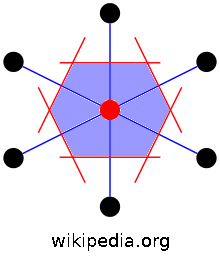
\includegraphics[width=2cm]{glossary/images/wsc.png}}}
}
\newglossaryentry{brillouinzone}
{
    name={Brillouin Zone},
    description={the Wigner-Seitz cell in reciprocal space}
}

\newglossaryentry{wavefunction}
{
    name={wave function},
    description={contains all there is to know about a system and it's meaning is given by a probability ${\lvert \Psi \rvert}^2 = 1 $}
}

\newglossaryentry{planewave}
{
    name={plane wave},
    description={a wave of parallel planes of constant frequency that are normal to the direction of propagation}
}

\newglossaryentry{blochtheorem}
{
    name={Bloch theorem},
    description={electron wave functions may be written as a sum of plane waves $\psi_{\vec{k},n} \vec{r} = \sum c_{\vec{k} + \vec{G}, n} exp(i (\vec{k} + \vec{G}) \dot \vec{r})$}
}

\newglossaryentry{atomicunits}
{
    name={Atomic Units},
    description={length in Bohr - 1 bohr = 0.529 angstrom, energy in Hartree - 1 Hartree = 27.211 eV}
}
\newglossaryentry{jellium}
{
    name={jellium},
    description={quantum mechanical model of electrons distributed uniformly through space (homogeneous electron gas)}
}
\newglossaryentry{heg}
{
    name={homogeneous electron gas},
    description={quantum mechanical model of electrons distributed uniformly through space (jellium)}
}
\newglossaryentry{304SS}
{
    name={304SS},
    description={Austenitic stainless steel: 18-20\%Cr, 8-11\%Ni}
}
\newglossaryentry{316SS}
{
    name={316SS},
    description={Austenitic stainless steel: 16.5-18.5\%Cr, 10-13\%Ni, 2.0-2.5\%Mo}
}
\newglossaryentry{matrixdiagonalization}
{
    name={matrix diagonalization},
    description={Take matrix $A$ and find a diagonal matrix $D$ such that $S^-1 A S = D$}
}
\newglossaryentry{supercritical}
{
    name=supercritical,
    description={Above $374^{\circ}C$ (647K) and 22.1MPa water is no longer a distinct liquid or gas and it becomes supercritical}
}
\newglossaryentry{reduction}
{
    name=reduction,
    description={Gaining electrons or loss of oxygen}
}
\newglossaryentry{oxidation}
{
    name=oxidation,
    description={Losing electrons or gaining oxygen}
}
\newglossaryentry{cathode}
{
    name=cathode,
    description={Electrode where current enters from an electrolyte}
}
\newglossaryentry{anode}
{
    name=anode,
    description={Electrode where current leaves to an electrolyte}
}
\newglossaryentry{valenceelectron}
{
    name=valence electron,
    description={outer shell electron that can form bonds}
}
\newglossaryentry{kohnshameq}
{
    name=Kohn-Sham equations,
    description={$\hat{v}_{KS}(\vec{r_e}, \vec{r_n}) = v_{n-e}(\vec{r_e}, \vec{r_n}) + \int d^3\vec{r'} \frac{\rho(\vec{r_{e}'})}{\lvert \vec{r_{e}} - \vec{r_{e}'}} + v_{xc}[\rho](\vec{r_{e}})$}
}
\newglossaryentry{pauliexp}
{
    name=Pauli exclusion principle,
    description={half-integer spin particles cannot have the same quantum numbers}
}
\newglossaryentry{paulivector}
{
    name=Pauli vector,
    description={sum of the three Pauli matrices $\vec{\sigma} = \begin{bmatrix} 0 & 1 \\ 1 & 0\end{bmatrix} + \begin{bmatrix} 0 & -i \\ i & 0\end{bmatrix} + \begin{bmatrix} 1 & 0 \\ 0 & -1\end{bmatrix}$}
}
\newglossaryentry{fermion}
{
    name=fermion,
    description={half-integer spin particle - includes electrons, protons, neutrons}
}
\newglossaryentry{boson}
{
    name=boson,
    description={integer spin particle - includes photons, gluons}
}
\newglossaryentry{proofstrength}
{
    name=proof strength,
    description={stress at which a material undergoes a permanent extension}
}
\newglossaryentry{youngsmodulus}
{
    name=Young's modulus,
    description={measure of resistance to elastic deformation $\delta = \frac{\text{stress}}{\text{strain}}$}
}
\newglossaryentry{yieldstrength}
{
    name=yield strength,
    description={maximum stress before permanent deformation occurs}
}
\newglossaryentry{ultimatetensilestrength}
{
    name=ultimate tensile strength,
    description={maximum stress the material can withstand}
}
\newglossaryentry{allotrope}
{
    name=allotrope,
    description={an element that exists in multiple forms/structures - the common example of allotropes are graphite (hexagonal sheets) and diamond (regular tetrahedral structure) for carbon}
}
\newglossaryentry{obsstable}
{
    name=observationally stable,
    description={theoretically unstable but yet to be measured as unstable by experiment}
}




%%%%%%%%%%%%%%%%%%%%%%%%%%%%%%%%%%%
% Elements
%%%%%%%%%%%%%%%%%%%%%%%%%%%%%%%%%%%

\newglossaryentry{C}
{
    name=C,
    description={Carbon $Z = 6$, $A_r = 12.00$}
}
\newglossaryentry{O}
{
    name=O,
    description={Oxygen $Z = 8$, $A_r = 16.00$}
}
\newglossaryentry{Mg}
{
    name=Mg,
    description={Magnesium $Z = 12$, $A_r = 24.30$}
}
\newglossaryentry{Al}
{
    name=Al,
    description={Aluminium $Z = 13$, $A_r = 26.98$}
}
\newglossaryentry{P}
{
    name=P,
    description={Phosphorus $Z = 15$, $A_r = 30.97$}
}
\newglossaryentry{Cr}
{
    name=Cr,
    description={Chromium $Z = 24$, $A_r = 52.00$}
}
\newglossaryentry{Mn}
{
    name=Mn,
    description={Maganese $Z = 25$, $A_r = 54.94$}
}
\newglossaryentry{Fe}
{
    name=Fe,
    description={Iron $Z = 26$, $A_r = 55.85$}
}
\newglossaryentry{Co}
{
    name=Co,
    description={Cobalt $Z = 27$, $A_r = 58.93$}
}
\newglossaryentry{Ni}
{
    name=Ni,
    description={Nickel $Z = 28$, $A_r = 58.69$}
}
\newglossaryentry{Cu}
{
    name=Cu,
    description={Copper $Z = 29$, $A_r = 63.55$}
}
\newglossaryentry{Zn}
{
    name=Zn,
    description={Zinc $Z = 30$, $A_r = 65.38$}
}
\newglossaryentry{Zr}
{
    name=Zr,
    description={Zirconium $Z = 40$, $A_r = 91.22$}
}
\newglossaryentry{Mo}
{
    name=Mo,
    description={Molybdenum $Z = 42$, $A_r = 95.95$}
}
\newglossaryentry{Ru}
{
    name=Ru,
    description={Ruthenium $Z = 44$, $A_r = 101.07$}
}
\newglossaryentry{Pd}
{
    name=Pd,
    description={Palladium $Z = 46$, $A_r = 106.42$}
}
\newglossaryentry{Cs}
{
    name=Cs,
    description={Caesium $Z = 55$, $A_r = 132.91$}
}
\newglossaryentry{W}
{
    name=W,
    description={Tungsten $Z = 74$, $A_r = 183.84$}
}
\newglossaryentry{Ir}
{
    name=Ir,
    description={Iridium $Z = 77$, $A_r = 192.22$}
}
\newglossaryentry{Pt}
{
    name=Pt,
    description={Platinum $Z = 78$, $A_r = 195.08$}
}
\newglossaryentry{Th}
{
    name=Th,
    description={Thorium $Z = 90$, $A_r = 232.04$}
}
\newglossaryentry{U}
{
    name=U,
    description={Uranium $Z = 92$, $A_r = 238.03$}
}
\newglossaryentry{Pu}
{
    name=Pu,
    description={Plutonium $Z = 94$, $A_r = 244$}
}


%%%%%%%%%%%%%%%%%%%%%%%%%%%%%%%%%%%
% Radiation Units
%%%%%%%%%%%%%%%%%%%%%%%%%%%%%%%%%%%

\newglossaryentry{becquerel}
{
    name=Becquerel,
    description={Becquerel (Bq) - decays per second}
}
\newglossaryentry{curie}
{
    name=Curie,
    description={Curie (Ci) - activity of 1 gram of Radium-226 - 1Ci = $3.7 \times 10^{10}$ decays per second}
}
\newglossaryentry{rutherford}
{
    name=Rutherford,
    description={Rutherford (Rd) - $1.0 \times 10^{6}$ decays per second}
}
\newglossaryentry{rontgen}
{
    name=Rontgen,
    description={Rontgen (R) - a measure of electric charge freed per unit mass of air - $1R = 2.58 \times 10^{-4} C/kg$}
}
\newglossaryentry{gray}
{
    name=Gray,
    description={Gray (Gy) how much energy is deposited into matter and 1Gy is equal to 1 Joule per kg}
}
\newglossaryentry{rad}
{
    name=Rad,
    description={Rad (Rad) this is another measure for absorbed dose and 1 rad is equal to 100 ergs per gram (1 rad = 1.0cGy = 0.01Gy)}
}
\newglossaryentry{sievert}
{
    name=Sievert,
    description={Sievert (Sv) - equivalent/effective dose - this is the absorbed dose with radiation weighting (equivalent) and tissue weighting (effective) factors applied $1Sv \text{(equivalent)} = 1 J/kg \times W_r$ and $1Sv \text{(effective)} = 1 J/kg \times W_r \times W_t$}
}
\newglossaryentry{rem}
{
    name=Rontgen Equivalent Man,
    description={Rontgen Equivalent Man (REM) - equivalent/effective dose - 1 REM equivalent is equal to $1Rad \times W_r$ (1cGy $1Rad \times W_r$) and 1 REM effective is equal to $1Rad \times W_r \times W_t$ (1cGy $1Rad \times W_r \times W_t$)}
}
\newglossaryentry{ld50}
{
    name=LD50,
    description={Lethal dose in 50 percent of cases}
}
\newglossaryentry{barn}
{
    name=barn,
    description={Unit for cross sectional area ($1.0 \times 10^{28} m^{2}$)}
}
\newglossaryentry{meanfreepath}
{
    name=mean free path,
    description={average (mean) distance a projectile travels before reacting with the target}
}



\newacronym{kerma}{KERMA}{Kinetic Energy Released per unit MAss}

\newacronym{gif}{GIF}{Generation IV International Forum}
\newacronym{geniv}{GenIV}{Generation IV}


\newacronym{gen1}{Gen I}{Generation I}
\newacronym{gen2}{Gen II}{Generation II}
\newacronym{gen2+}{Gen II+}{Generation II+}
\newacronym{gen3}{Gen III}{Generation III}
\newacronym{gen3+}{Gen III+}{Generation III+}
\newacronym{gen4}{Gen IV}{Generation IV}

\newacronym{pwr}{PWR}{Pressurised Water Reactor}
\newacronym{lwr}{LWR}{Light Water Reactor}
\newacronym{bwr}{BWR}{Boiling Water Reactor}
\newacronym{agr}{AGR}{Advanced Gas Reactor}
\newacronym{vver}{VVER}{Vodo-Vodyanoi Energetichesky Reaktor}
\newacronym{rbmk}{RBMK}{Reaktor Bolshoy Moshchnosti Kanalnyy}
\newacronym{candu}{CANDU}{Canada Deuterium Uranium}
\newacronym{epr}{EPR}{European Pressurised Reactor}
\newacronym{abwr}{ABWR}{Advanced Boiling Water Reactor}
\newacronym{gfr}{GFR}{Gas-Cooled Fast Reactor}
\newacronym{lfr}{LFR}{Lead-Cooled Fast Reactor}
\newacronym{msr}{MSR}{Molten Salt Reactor}
\newacronym{scwr}{SCWR}{Supercritical-Water-Cooled Reactor}
\newacronym{sfr}{SFR}{Sodium-Cooled Fast Reactor}
\newacronym{vhtr}{VHTR}{Very-High-Temperature Reactor}
\newacronym{fnr}{FNR}{Fast-Neutron Reactors}
\newacronym{elsy}{ELSY}{European Lead Fast Reactor}
\newacronym{fbr}{FBR}{Fast Breeder Reactor}
\newacronym{pbr}{PBR}{Pebble-Bed Reactor}
\newacronym{npp}{NPP}{Nuclear Power Plant}
\newacronym{ebr}{EBR}{Experimental Breeder Reactor}
\newacronym{iter}{ITER}{International Thermonuclear Experimental Reactor}
\newacronym{hpr}{HPR}{Hualong Pressurised Water Reactor}

\newacronym{ecis}{ECIS}{Equations Couplées Itérations Séquentielle}


\newacronym{triso}{TRISO}{Tristructural Isotropic}

\newacronym{ccgt}{CCGT}{Combined Cycle Gas Turbine}


\newacronym{endf}{ENDF}{Evaluated Nuclear Data File}
\newacronym{nea}{NEA}{Nuclear Energy Agency}
\newacronym{jeff}{JEFF}{Joint Evaluated Fission and Fusion File}
\newacronym{tendl}{TENDL}{TALYS-based Evaluated Nuclear Data Library}


\newacronym{sc}{SC}{Simple Cubic}
\newacronym{bcc}{BCC}{body centered cubic}
\newacronym{fcc}{FCC}{face centered cubic}
\newacronym{fct}{FCT}{face centered tetragonal}
\newacronym{cph}{CPH}{face centered tetragonal}
\newacronym{hcp}{HCP}{hexagonal close packed}
\newacronym{zb}{ZB}{zinc blende}


\newacronym{mcnp}{MCNP}{Monte Carlo N-Particle}

\newacronym{hrb}{HRB}{Hardness Rockwell B}


\newacronym{md}{MD}{molecular dynamics}
\newacronym{akmc}{akMC}{atomic kinetic Monte Carlo}
\newacronym{lammps}{LAMMPS}{Large-scale Atomic/Molecular Massively Parallel Simulator}


\newacronym{nist}{NIST}{National Institute of Standards and Technology}

\newacronym{fs}{FS}{Finnis-Sinclair}
\newacronym{eam}{EAM}{embedded-atom method}
\newacronym{2beam}{2BEAM}{two band embedded-atom method}
\newacronym{meam}{MEAM}{modified embedded-atom method}

\newacronym{hf}{HF}{Hartree-Fock}

\newacronym{dft}{DFT}{Density Functional Theory}
\newacronym{scf}{SCF}{self consistent field}
\newacronym{pbe}{PBE}{Perdew-Burke-Ernzerhof}
\newacronym{pbesol}{PBESOL}{Perdew-Burke-Ernzerhof functional revised for solids}
\newacronym{pz}{PZ}{Perdew-Zunger}
\newacronym{lda}{LDA}{local density approximation}
\newacronym{lsda}{LSDA}{local spin density approximation}
\newacronym{gga}{GGA}{generalized gradient approximation}
\newacronym{zbl}{ZBL}{Ziegler-Biersack-Littmark}

\newacronym{igscc}{IGSCC}{inter granular stress corrosion cracking}
\newacronym{tgscc}{TGSCC}{trans granular stress corrosion cracking}
\newacronym{iascc}{IASCC}{irradiation assisted stress corrosion cracking}
\newacronym{scc}{SCC}{stress corrosion cracking}
\newacronym{ris}{RIS}{radiation induced segregation}
\newacronym{rip}{RIP}{radiation induced precipitation}

\newacronym{dpa}{DPA}{displacements per atom}
\newacronym{vpi}{VPI}{vacancies per ion}
\newacronym{pka}{PKA}{primary knock-on atom}


\newacronym{edf}{EDF}{Électricité de France}


\newacronym{cpu}{CPU}{central processing unit}
\newacronym{gpu}{GPU}{graphical processing unit}

\newacronym{pgm}{PGM}{platinum group metal}


\newacronym{ornl}{ORNL}{Oak Ridge National Laboratory}
\newacronym{linac}{LINAC}{linear accelerator}
\newacronym{sns}{SNS}{Spallation Neutron Source}
\newacronym{rfq}{RFQ}{Radio Frequency Quadrupole}
\newacronym{hfir}{HFIR}{High Flux Isotope Reactor}
\newacronym{slac}{SLAC}{Stanford Linear Accelerator Center}
\newacronym{triumf}{TRIUMF}{TRI-University Meson Facility}
\newacronym{lhc}{LHC}{Large Hadron Collider}
\newacronym{cern}{CERN}{Conseil Européen pour la Recherche Nucléaire}
\newacronym{nbs}{NBS}{National Bureau of Standards}
\newacronym{nbsr}{NBSR}{National Bureau of Standards Reactor}
\newacronym{avf}{AVF}{Azimuthally Varying Field}
\newacronym{iaea}{IAEA}{International Atomic Energy Agency}


\newacronym{ins}{INS}{Institute for Nuclear Study}



\newacronym{mox}{MOX}{mixed oxide}

\newacronym{srim}{SRIM}{Stopping Range In Matter}
\newacronym{exyz}{EXYZ}{Energy, x, y, z}
\newacronym{trim}{TRIM}{TRansport In Matter}
\newacronym{nds}{NDS}{Nuclear Data Services}

\newacronym{omp}{OMP}{optical model potential}
\newacronym{nomp}{NOMP}{nuclear optical model potential}


\newacronym{exfor}{EXFOR}{EXchange FORmat}


\newacronym{bca}{BCA}{binary collision approximation}

\newacronym{uts}{UTS}{Ultimate Tensile Strength}


\newacronym{tise}{TISE}{Time Independent Schr\"{o}dinger Equation}
\newacronym{hk}{HK}{Hohenberg-Kohn}
\newacronym{ks}{KS}{Kohn-Sham}
\newacronym{xc}{XC}{exchange-correlation}


\newacronym{ng}{NG}{Newton-Gauss}
\newacronym{lma}{LMA}{Levenberg-Marquardt Algorithm}
\newacronym{bfgs}{BFGS}{Broyden Fletcher Goldfarb Shanno}
\newacronym{lmbfgs}{LM-BFGS}{Limited-memory Broyden Fletcher Goldfarb Shanno}
\newacronym{nm}{NM}{Nelder Mead}
\newacronym{sa}{SA}{Simulated Annealing}
\newacronym{bh}{BH}{Basin Hopping}
\newacronym{cg}{CG}{Conjugate Gradient}
\newacronym{qp}{QP}{Quadratric Programming}




\newacronym{mpi}{MPI}{Message Parsing Interface}
\newacronym{openmp}{OpenMP}{Open Multi-Processing}



\newacronym{ecp}{ECP}{electrochemical corrosion potential}

\newacronym{eos}{EOS}{equation of state}
\newacronym{ec}{EC}{elastic constants}
\newacronym{mskp}{MSKP}{Mehl, Singh, Klein, Papaconstantopoulos}
\newacronym{rfkj}{RFKJ}{Ravindran, Fast, Korzhavyi, Johansson}

\newacronym{dna}{DNA}{Deoxyribonucleic Acid}


\newacronym{ke}{KE}{Kirkendall effect}
\newacronym{ike}{IKE}{inverse Kirkendall effect}

\newacronym{asme}{ASME}{American Society of Engineers}

\newacronym{sem}{SEM}{scanning electron microscope}
\newacronym{tem}{TEM}{transmission electron microscope}
\newacronym{stem}{STEM}{scanning transmission electron microscope}
\newacronym{sims}{SIMS}{secondary-ion mass spectrometry}
\newacronym{naa}{NAA}{neutron activation analysis}

\newacronym{bz}{BZ}{Brillouin zone}
\newacronym{ibz}{IBZ}{irreducible Brillouin zone}


\newacronym{rss}{RSS}{residual squared sum}

\newacronym{url}{URL}{Uniform Resource Locator}
\newacronym{www}{WWW}{World Wide Web}

\newacronym{uk}{UK}{United Kingdom}
\newacronym{usa}{USA}{United States of America}
\newacronym{ussr}{USSR}{United Socialist Soviet Republic}


\makeglossaries


\newcommand{\changefont}{%
    \fontsize{8}{11}\selectfont
}
\fancyhf{}
\fancyhead[LE,RO]{\changefont \slshape \rightmark} %section
\fancyhead[RE,LO]{\changefont \slshape \leftmark} %chapter
\fancyfoot[C]{\changefont \thepage} %footer

\pagestyle{fancy}
%\pagestyle{plain}





\begin{document}


\begin{titlepage}
  \begin{center}   
    \centerline{
\includegraphics[width=0.7\textwidth]{cover/Cover_Art}}    
    
    
    \textbf{Department of Metallurgy \& Materials}   
    
    \vspace*{2.0cm}       
    \Large{}    
    \textbf{Irradiation Damage Simulations of Platinum Group Metal Modified Austenitic Stainless Steels for Reactor Core Components}
    \vspace{0.8cm}   
    \normalsize{}
    
    \text{by}
    \text{Ben Palmer}    
    \vfill        
    \text{A thesis submitted to the University of Birmingham}
    \text{for the degree of Doctor of Philosophy}
    
    \text{Supervised by Dr Brian J Connolly, Dr Mark S D Read and Prof Alessandro Mottura}
  \end{center}
\end{titlepage}

\afterpage{\blankpage}


%% Cover + Abstract
\pagenumbering{gobble}

\pagenumbering{roman} 
\begin{abstract}
Austenitic stainless steels have been used since the early days of nuclear power and they will play an important role in the construction of \acrfull{gen3+} and \acrfull{gen4} plant designs.  Materials used in future reactor designs will need to withstand more extreme conditions whilst improving upon safety.  Neutron damage is a major contributor to material failure for many complex reasons.  

It is known that radiation damage depletes Chromium at the grain boundary.  As Chromium is a key element in giving stainless steel its corrosion resistance, a depletion of it leads to \acrfull{igscc}.  Corrosion may also be prevented by adding small amounts of Palladium and Ruthenium to the steel, but this may or may not be affected by neutron damage.

Irradiation of components using neutrons is expensive with relatively few high flux reactors available, but even with these reactors it is difficult to speed up the damage process appreciably.  A proton beam may be used to emulate neutron damage at a much faster rate and it is also possible to model radiation damage using a computer.  

Radioactive waste is created in a reactor when neutrons activate isotopes that make up the components within.  This is also true where a light ion beam is used in place of neutrons.  The relationship between the ion beam parameters and the component being irradiated is complex and depends upon the type and energy of the projectile, the thickness of the target and its constituent isotopes.

A modified Bateman equation was derived to calculate the radioactivity of a proton irradiated target and a computer program (Activity) was created to implement the calculation using evaluated nuclear reaction cross section data.  The program has been compared to data measured from the irradiation of an iron sample using the University of Birmingham cyclotron.  It was also used to model the radioactivity of a target irradiated to 100 \acrfull{dpa} at a range of beam energies in order to minimise both the irradiation time and radioactive waste.  The results show an increase in target activity of 3 orders of magnitude for a 25MeV proton beam when compared to a 10MeV proton beam.

Interatomic potentials are required to model radiation damage and its effect using \acrfull{md} or \acrfull{akmc}.  Platinum group metals \acrshort{pgm}s may be added to a stainless steel to improve corrosion resistance, importantly in conditions where chromium is depleted.  There are existing potentials for binary alloys of Iron and Palladium as well as for the pure elements Iron, Palladium and Ruthenium, but they are designed for use with particular crystal structures such as \acrfull{bcc} and \acrfull{hcp}.

In this work \acrfull{dft} is used to create a reference database that is needed for fitting Fe-Pd and Fe-Ru potentials.  As the material of interest is austenitic stainless steel, the reference database and potential are restricted to the \acrfull{fcc} crystal structure.  The potential type is a many body \acrfull{eam} that also has a \acrfull{zbl} core potential in order to model collisions.

A computer program (EAMPA) was developed in Python and Fortran to fit potentials using the reference database and bulk properties.  The resulting potentials are a step towards \acrshort{md} and \acrshort{akmc} simulations of radiation damage in \acrshort{pgm} doped austenitic stainless steels.  They are also a step towards investigating whether or not radiation damage causes \acrshort{pgm}s to deplete or enrich at grain boundaries, showing whether or not their corrosion resistance is removed or retained.  
\end{abstract}

%% Tables of...
\tableofcontents
\listoffigures
\listoftables



%% Chapters of Thesis
\pagenumbering{arabic}



%%##################################################################
%% Introduction
%%##################################################################

\chapter{Introduction}

\begin{changemargin}{1.0cm}{1.0cm} 
\abstractpreamble{Several \acrshort{gen3+} nuclear reactors have been proposed for construction in the UK (with Hinckley Point C now under construction) and \acrshort{gen4} nuclear reactors are being researched and developed.  New materials are required to withstand the extreme conditions in and around the core of these reactors.  Austenitic stainless steels have been an important structural material in the industry, and may continue to be so, providing the problem of \acrfull{igscc} can be addressed.  Doping these steels with \acrfull{pgm}s has been seen to reduce \acrshort{igscc}, but the effects on corrosion resistance are unknown for these steels when irradiated by a radiation field.\\
\\
Since writing this thesis, Hinkley Point B has now been retired.  References to it being in operation were correct at the time.}
\end{changemargin}

 
%Notes:
%brief history of nuclear power
%discuss neutron spectra focussing on u-235 fission
%what materials are used in nuclear power - considerations (damage, transmutation, costs, other environmental factors)
%focus on austenitic stainless steels


%%%%%%%%%%%%%%%%%%%%%%%%%%%%%%%%%%%%%%%%%%%%%%%%%%%%%%%%%%%%%%%%%%%%%%%%%%%%%%%%%%%%%%%%%%%%%%%%%%%%%%%%%%
%%
%%  MOTIVATION
%%
%%%%%%%%%%%%%%%%%%%%%%%%%%%%%%%%%%%%%%%%%%%%%%%%%%%%%%%%%%%%%%%%%%%%%%%%%%%%%%%%%%%%%%%%%%%%%%%%%%%%%%%%%%

\section{Motivation}

I have often questioned the motivation behind this work, and at times it has been a challenge to see the wood through the trees.  To help me focus throughout I would restate the motivation and objectives to myself.

Mass produced steels are not perfect repeating crystals, but are made up of small grains.  \Gls{Cr} is added to steel to make stainless steel, and this is more resistant to corroding than steel.  When steel is in a nuclear reactor, it will have to perform under extreme conditions, such as:

\begin{itemize}
\item high temperatures
\item strain cause by high pressures and radiation induced swelling
\item radiation damage and strains resulting from this damage
\item a changing environment, for example radiolysis of water and transmutation of isotope due to radiation
\item corrosive environments while in the reactor
\item corrosive environments out of the reactor (e.g. fuel cladding in storage)
\end{itemize}

Radiation damages the steel in a number of ways, including directly knocking atoms out of their place within the lattice structure of the crystalline grains that make up the steel as well as changing the isotopes that make up the steel into new isotopes.  An example of the latter is a neutron reacting with an \Gls{Fe} atom, transmuting it into a \Gls{Co} atom.

In time, the radiation damage causes the percentage of Cr at the surface of the grains to drop, and as it falls the steel loses its protection from corrosion at the boundary between the grains it is made of.  

This work is divided into two parts.

\subsection{Part 1: Activity Computer Program}

The materials must be tested before being used in a nuclear reactor.  One way to do this would be to place samples of the steel into a test reactor.  This is expensive and, as a by-product, the steel sample becomes radioactive.  It is difficult to create a large number of neutrons, but it is much easier, and cheaper, to create a beam of protons.  Protons can be accelerated in a machine such as the Cyclotron at the University of Birmingham.  

The damage that protons cause to a sample is not precisely the same as that cause by neutrons, but it is a cheaper alternative and is a trade-off between the cost and results.  One side effect that proton irradiation shares with neutron irradiation is the creation of radioactive waste.  

The first part of this work investigates exactly how radioactive a samples becomes when irradiated with a proton beam.  An existing set of equations, named after Mathematician Harry Bateman, were modified and a computer program was created to perform the calculation.  The user inputs the constituent elements that make up the material, the ratio of these elements, and the irradiation settings.  The program then estimates how radioactive the sample will be and the predicted gamma energies.


\subsection{Part 2: Iron-Palladium and Iron-Ruthenium Potential}

The addition of \Gls{Cr} to make stainless steel is not the only way to make a steel resistant to corrosion.  Adding metals such as \Gls{Mo}, \Gls{Pd} and \Gls{Ru} to steel can increase the resistance to corrosion, but Mo is several hundred times the cost of Fe ore, and Pd is thousands of times as expensive.

Simulating radiation damage using a computer is now a feasible and sensible way to investigate how these materials will be affected by radiation damage, and the simulations may reveal insights that experiments are not able to show, either because they happen on too small a timescale or within the material at too small a length scale.

Key to the simulations success is being able to accurately calculate how the atoms interact with one another.  The second part of this work concentrates on deriving a mathematical description of how Pd \& Fe and Ru \& Fe atoms interact with one another, which would then allow future simulations of steel with small amounts of Pd or Ru added to it.

Radiation causes Cr to be depleted at the grain boundary.  If these simulations go on to show that Pd and Ru are not depleted, it would suggest that the corrosion resistance is maintained despite the decrease in the amount of Cr at the grain boundary due to radiation damage.


%%%%%%%%%%%%%%%%%%%%%%%%%%%%%%%%%%%%%%%%%%%%%%%%%%%%%%%%%%%%%%%%%%%%%%%%%%%%%%%%%%%%%%%%%%%%%%%%%%%%%%%%%%
%%
%%  BRIEF HISTORY, PRESENT AND FUTURE
%%
%%%%%%%%%%%%%%%%%%%%%%%%%%%%%%%%%%%%%%%%%%%%%%%%%%%%%%%%%%%%%%%%%%%%%%%%%%%%%%%%%%%%%%%%%%%%%%%%%%%%%%%%%%


\FloatBarrier
\section{Nuclear Power in the United Kingdom}

\subsection{Nuclear Fuel}

The primary fuel of commercial nuclear power stations since those first built in the 1950s has been \Gls{U}.  ${}^{235}_{92}U$ is \gls{fissile} and fissions with a high probability when thermal neutrons are captured, due to its very high thermal neutron fission cross section (fig. \ref{figure:u235u238fissionxs}).

\begin{figure}[tbp]
  \begin{center}
    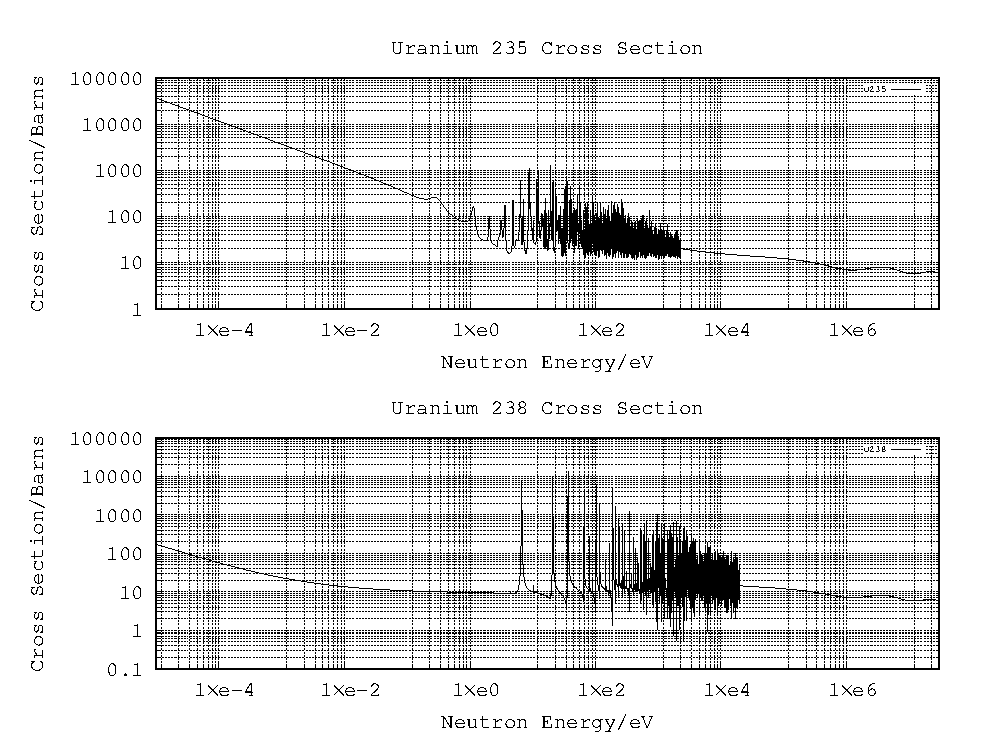
\includegraphics[width=.8\linewidth]{chapters/introduction/plots/uranium_cross_section/u_xs}%
    \caption{U-235 and U-238 Fission Cross Sections}
    \label{figure:u235u238fissionxs}
  \end{center}
\end{figure}

Natural U contains a small percentage of fissile ${}^{235}_{92}U$ (0.7\%) with the rest being its heavier isotope, ${}^{238}_{92}U$.  This heavier isotope is fissionable, but its fission cross section is much lower than ${}^{235}_{92}U$ (fig. \ref{figure:u235u238fissionxs}).  Many of the design considerations for reactors in operation revolve around the amount of ${}^{235}_{92}U$ there is in the fuel and having a sufficient flux of thermal neutrons passing through the fuel to sustain a reaction.

A number of \acrshort{gen4} designs use the fast neutron spectrum to fission ${}^{238}_{92}U$ and other fuels such as ${}^{232}_{90}Th$ to generate energy and breed other fissile isotopes (${}^{233}_{92}U$).  By moving away from ${}^{235}_{92}U$, this increases the potential fuel stockpile, but also brings its own set of challenges.


\FloatBarrier

\subsection{Generation I Reactors}

The first generation reactors were primarily prototype reactors.  They included graphite moderated reactors, light water and heavy water reactors.  Early reactors were designed to produce electricity, but also fissile material for nuclear weapons.  With a power output of less than 2MW, the Gen I power station Calder Hall generated much less electricity than a modern nuclear power plant which may produce 1GW per reactor.  It did, however, produce \Gls{Pu} for the UK's nuclear weapon programme.

Magnox type reactors were the first used in the \acrshort{uk}.  These reactors used natural U as a fuel and were carefully designed to produce energy despite using an un-enriched fuel.  Graphite was used as a moderator, and the low neutron capture cross section of the Magnox \Gls{Mn} alloy cladding allowed a nuclear reaction to occur despite the fuel not being enriched.

In all there were 11 Magnox power stations built in the UK with 26 reactors in total.  Construction of the first commercial reactor in the UK, Calder Hall, started in 1953 and it operated from 1956 to 2003.  All have now shut down with the last, Wylfa in Anglesey, closing in 2015.

\subsection{Generation II Reactors}

\acrshort{gen2} marked the transition from prototype reactors to higher powered commercial reactors.  There were a number of designs including the \acrshort{agr}, a graphite core $CO_2$ cooled reactor, that was implemented in the UK.  Light water reactors included the \acrshort{pwr} and \acrshort{bwr} in the west and the \acrshort{vver} in the \acrshort{ussr}.  The \acrshort{rbmk} was a graphite moderated reactor used in the \acrshort{ussr} and the \acrshort{candu} a heavy water reactor designed and used in Canada.

There are many of these reactors from this period still in operation around the world, and there have been recent implementations of these designs.  There are 15 reactors currently operating in the UK, and they are all \acrshort{gen2} reactors.  Of these, 14 are \acrshort{agr} and 1, Sizewell B, is a \acrshort{pwr} (fig. \ref{fig:remainingreactorsuk}).

\begin{figure}[tbp]
  \begin{center}
    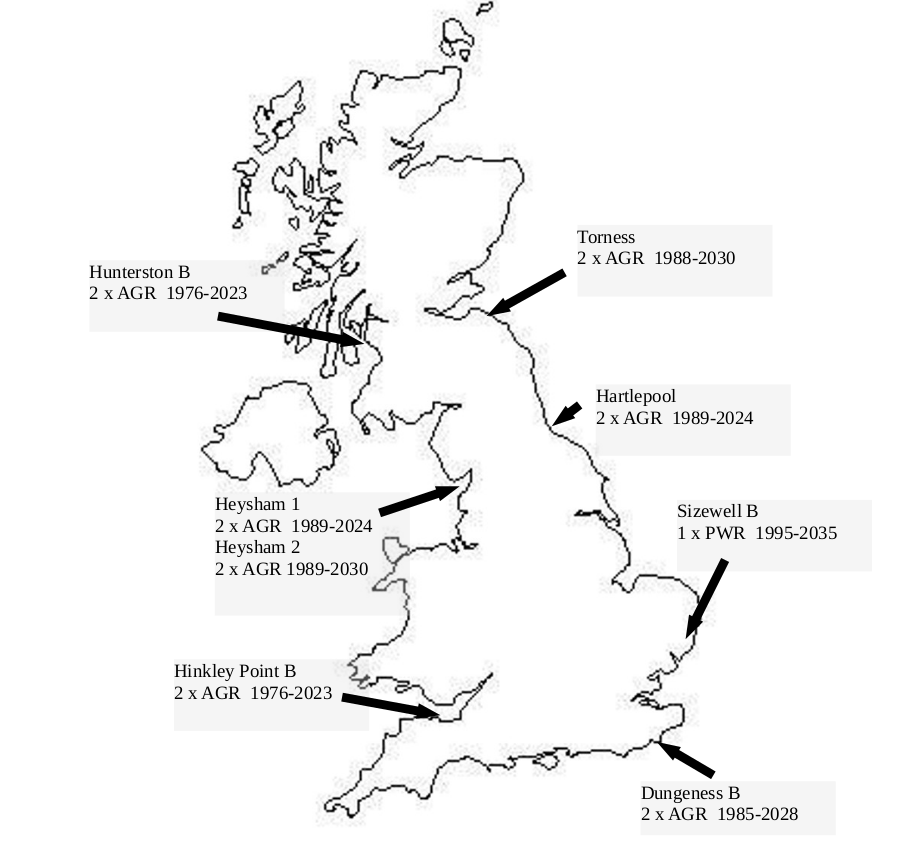
\includegraphics[width=12.0cm]{chapters/introduction/images/remaining_plants.png}
    \captionsetup{font={it}}
    \caption{Remaining reactor locations in the UK}
    \label{fig:remainingreactorsuk}
  \end{center}
\end{figure}

The planned life span for this generation of reactor was 30-40 years, although this has now been extended to 50-60 years in some cases.  The \acrshort{agr} reactors in the UK have been operational for over 40 years, and by the time Hunterston B and Hinkley Point B are planned to be decommisioned, they will have been operational for 46 years.  Designed with safety improvements in mind over Gen I reactors, they were also intended to produce more power with less of a focus on producing fissile material for weapons.  Unfortunately, this generation of reactors had the worst track record of any regarding safety, with Three Mile Island, Fukashima and Chernobyl all being \acrshort{gen2} designs.

\acrshort{gen2+} reactors have been built recently with 18 CPR-1000s being constructed over the last decade in China.  The UK is currently looking towards \acrshort{gen3+} reactors while \acrshort{gen4} proposals are being researched.   


\subsection{Generation III Reactors}

There are no \acrshort{gen3} reactors operating in the UK.  The first was built in Japan in 1996 and the type of reactor installed was an \acrfull{abwr}.  Bradwell B is a proposed site for the \acrshort{gen3} Hualong One type \acrshort{pwr} power plant (\acrshort{hpr}1000), and if this goes ahead it would have an expected opening date between 2030-2035.   

This generation of reactor was designed to exceed the service life of the previous generation, and generate power for at least 60 years.  The safety features have been improved and include increased resilience to external factors, including accidental or intentional aircraft collision into the plant\cite{genIIIimprovements}.

\acrshort{gen3+} reactors go further in adding passive safety features, such as natural circulation and gravity coolant feed \cite{geniiiplussafety}.  Other aims of future generations are to standardise and simplify designs whilst improve the economy over \acrshort{gen2+} and \acrshort{gen3}. 


\section{An Approaching Energy Gap for the UK}

Since Calder Hall, the first commercial nuclear power plant, opened in 1956, the demand on electrical power generation in the UK has tripled (fig \ref{fig:electricityusagesuk}).  There is now a reliance on cheap and clean power from nuclear reactors as these provide a quarter of our electricity.  There are sixteen reactors operational in the UK:  the Magnox reactor at Wylfa and the fourteen \acrshort{agr} reactors are due to be decommissioned by 2023\cite{gen4}, and the remaining \acrshort{pwr} reactor, Sizewell B, is expected to remain operational until 2035\cite{gen4}.

\begin{figure}[tbp]
  \begin{center}
    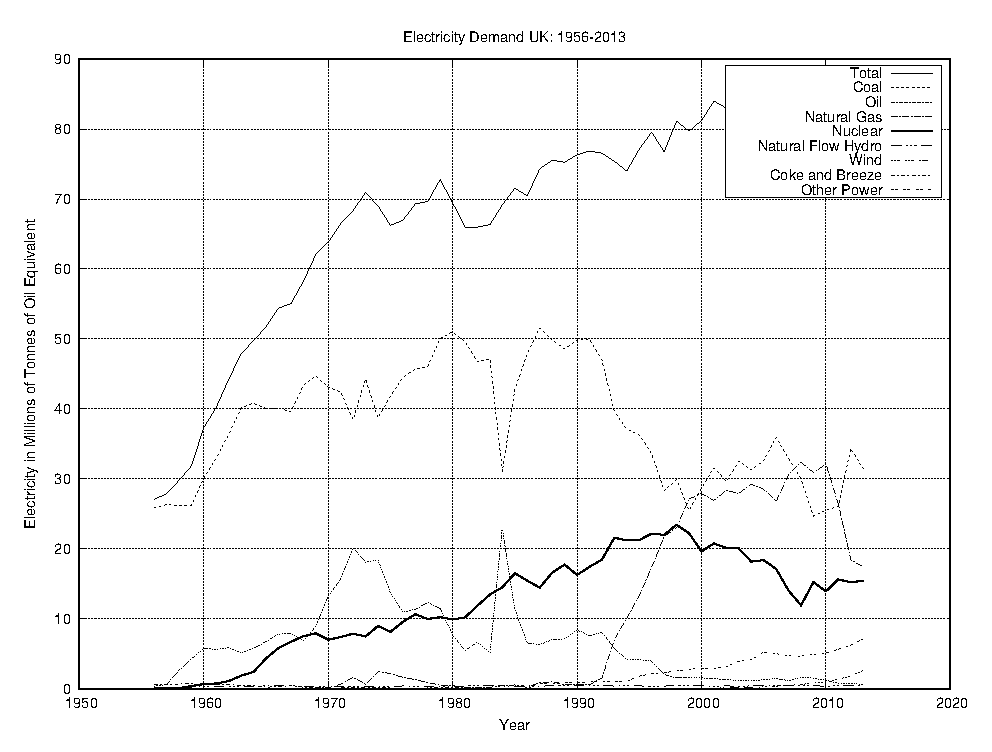
\includegraphics[width=.7\linewidth]{chapters/introduction/plots/elec_demand/elec_demand.eps}
    \captionsetup{font={it}}
    \caption{Electricity in Millions of Tonnes of Oil Equivalent}
    \label{fig:electricityusagesuk}
  \end{center}
\end{figure}

There is an obvious concern that within the next ten years the UK will lose a sizeable proportion of its electricity generation capabilities.  There are increasing pressures on countries to reduce their carbon dioxide output, so the gap created by ageing nuclear plants and coal power needs to be filled.


\subsection{Why choose Nuclear Power?}

As a civilization we need energy, whether it's in the form of electricity or stored chemically, and whilst we are becoming more efficient at using that energy, the demand for it will remain (unless something drastically changes our society).  There is a choice between burning fossil fuels or bio fuels, using energy from the Sun, wind, ground, oceans or rivers and finally using the energy of the nucleus, whether by fission or fusion.

Each has its drawbacks and advantages.  Renewable energies are unreliable; wind power only provides energy when there is a wind, and if the wind is too strong, they must be shut down or risk damage.  The Sun is only available for a portion of the day, and the duration and intensity change with the seasons, not to mention the impact of clouds on solar power.  Renewable sources are not very good at responding to demand; there isn't a button to turn up the power of the Sun, or increase the velocity of the wind when the national grid demands it.  If we were completely reliant on renewable energies, there would either need to be an efficient way to store energy on a large scale, or many more solar, wind, tidal and hydroelectric power stations than would be needed to produce excess energy.  Whilst the energy source may be free, turbines, solar panels, dams and so on require maintenance, so an excess of these would be wasteful and costly.

Fossil fuels release carbon dioxide, sulphur dioxide, naturally occurring trace radioactive elements and other pollutants into the atmosphere.  These power plants are useful because the fuel is cheap, but the waste is put back into the environment without much processing and the energy produce may be varied to meet the demand of the national grid.  

Nuclear power has a bad reputation with the public, in part caused by accidents such as the Windscale fire, Three Mile Island, Chernobyl, and Fukushima.  There have been examples of poor handling of nuclear waste in the past, such as the legacy storage ponds at Sellafield, and long term storage in geologically stable areas is something that hasn't been achieved to store the existing waste, let alone waste created in the future.

Modern nuclear power plants are very expensive to build, with the proposed 3.2GWe Sizewell C power plant expected to cost £20 billion or more \cite{ftnppcost}.  When compared to \textsterling0.5 billion for the 0.884GWe Carrington \acrshort{ccgt} Power Station \cite{efgccgtcost}, the initial costs are \textsterling0.57 billion per GWe for \acrshort{ccgt} compared to \textsterling6.25 billion per GWe for Nuclear.

There is an effort around the world of countries aiming to reduce the production of carbon dioxide as a result of burning fossil fuels.  When a power plant is operational, the carbon dioxide produced by nuclear power is negligible when compared with gas, oil and coal power plants.  

\begin{figure}[tbp]
  \begin{center}
    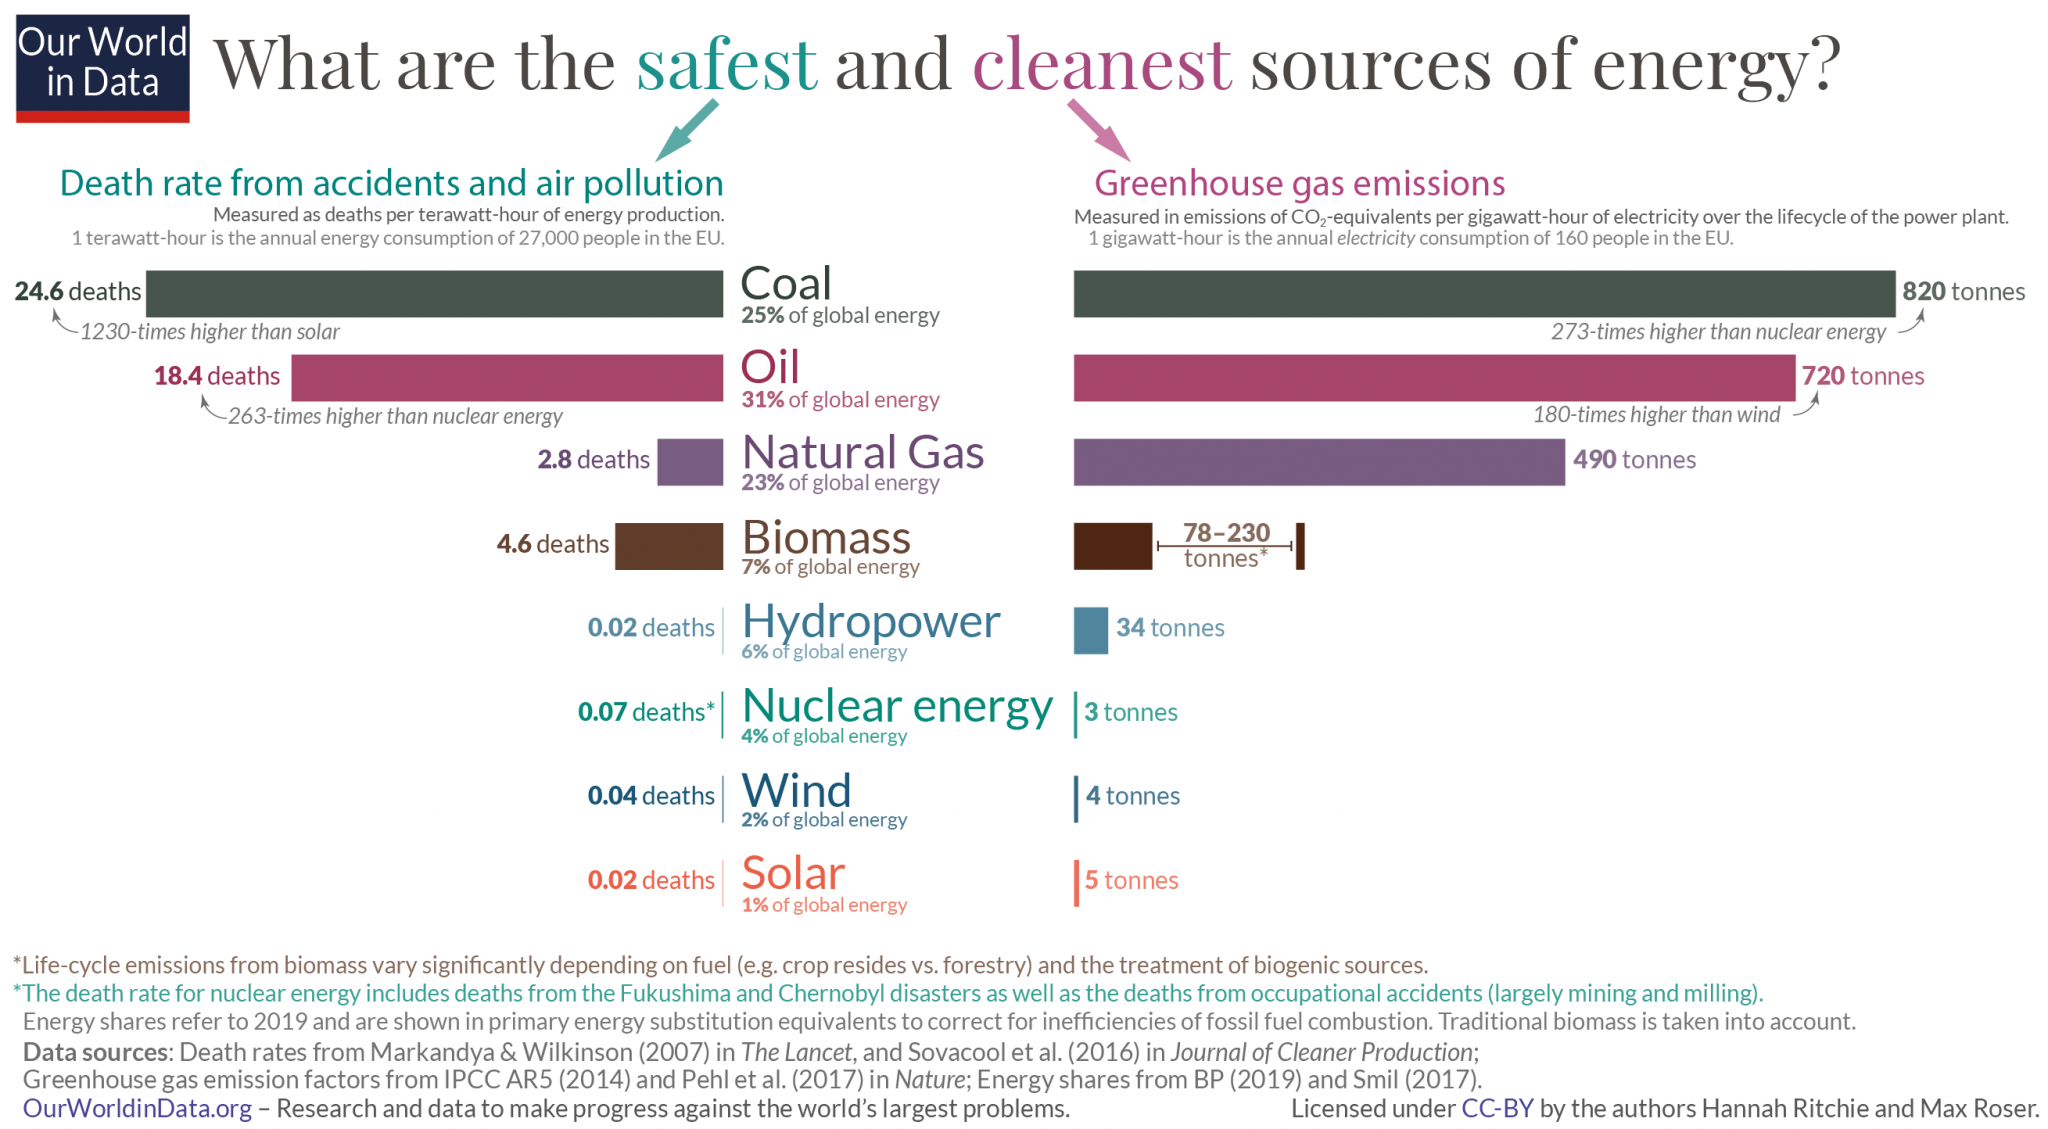
\includegraphics[width=.95\linewidth]{chapters/introduction/images/safest.png}
    \captionsetup{font={it}}
    \caption{Safest and cleanest sources of energy \cite{deathsfromenergysource} - deaths per terawatt hour and tonnes of CO\textsubscript{2} per gigawatt hour}
    \label{fig:safestenergy}
  \end{center}
\end{figure}

Despite its reputation amongst the public, nuclear is much safer than fossil fuels and is on par with renewable energies.  The pollution caused by fossil fuels affects us all and is responsible for many deaths each year, causing more misery than nuclear power ever has (fig. \ref{fig:safestenergy}).  Coal and oil are responsible for 350 and 260 times as many deaths as nuclear, respectively.

As a species, we have used combustion of chemicals to generate heat for thousands of years, culminating in high efficiency \acrshort{ccgt} power stations, with efficiencies above 60\%.  We are at the beginning of our journey with nuclear power, with many new and innovative designs proposed, where safety to plant workers and the general public are a priority.

Future designs may help to tackle the problematic waste generated in the past, and by using fertile material to produce fissionable elements other than ${}^{235}_{92}U$, the amount of fuel available to reactors will increase. 




\subsection{Planned and Under Construction in the UK}


Several sites have been acquired with the aim of building new nuclear power stations in the UK.  There are five sites and three reactor designs\cite{ocw01}:

\begin{itemize}
\item Hinkley Point: two Areva \acrshort{epr}s (EDF Energy), Hinkley Point C under construction
\item Sizewell: two Areva \acrshort{epr}s (EDF Energy)
\item Wylfa: 2-3 Hitachi \acrshort{abwr}s (Horizon Nuclear Power)
\item Oldbury: 2-3 Hitachi \acrshort{abwr}s (Horizon Nuclear Power)
\item Sellafield: 3 Westinghouse AP1000s (NuGeneration)
\ldots 
\end{itemize}

Two \acrshort{gen3+} reactors are under construction in the UK: Hinkley Point C 1 and C 2.  These reactors are Areva NP designed \acrshort{gen3+} \acrshort{epr}s, which are \acrshort{pwr}s, and the proposed opening years are 2025 and 2026 respectively.  

There are also plans to construct a third plant at Sizewell that, if accepted, will be an \acrshort{epr} reactor.  Sizewell C will join the decommissioned Sizewell A and operational Sizewell B, that may operate until 2055.




\subsection{Proposed Generation III+ Nuclear Power Plant Designs}


\subsubsection{Areva \acrshort{epr}}

The 1.6GW Areva \acrshort{epr} design has four primary loops transferring heat by pressurised water from the reactor to heat exchangers.  It requires U enriched to 5\% ${}^{235}_{92}U$ in the form of U Oxide Pellets.  The inlet temperature is $568.75K$ and the outlet temperature is $602.95K$.

There are 241 fuels assemblies, each containing 265 fuel rods giving a total of 63865 rods.  The fuel rod cladding is made from 316 stainless steel and has an inner diameter of 7.72mm and an outer diameter of 9.68mm.  The materials used to construct the control rod drive mechanisms includes 410 stainless steel and 304 stainless steel.

There are two \acrshort{epr} reactors planned for the proposed Sizewell C power plant.


\subsubsection{Westinghouse AP1000}

The 1.1GW Westinghouse AP1000 design is a pressurised water reactor with two primary loops transferring heat from the reactors to heat exchangers.  An enriched $UO_2$ fuel, up to 5\% ${}^{235}_{92}U$, is clad in Zirlo (a proprietary \Gls{Zr} alloy).  

Zirlo is an alternative cladding material to 316 stainless steel, and as a cladding material is absorbs fewer neutrons that steel cladding.  

\begin{table}[h]
\begin{center}
\renewcommand{\arraystretch}{1.2}
\begin{tabular}{c c c}
\hline\hline
Property & 316SS Fe 20Cr 8Ni 1Mo & Zirlo (Hill Approximaton) \\
\hline\hline
Bulk Modulus (GPa)     & 164.9 \cite{elasticprofecr}  & 98.5 \cite{crystengcommzirlo} \\
Shear Modulus (GPa)    & 74.6 \cite{elasticprofecr}   & 33.2 \cite{crystengcommzirlo} \\
Young's Modulus (GPa)  & 194.3 \cite{elasticprofecr}  & 89.7 \cite{crystengcommzirlo} \\
Poisson's Ratio        & 0.30 \cite{elasticprofecr}   & 0.35 \cite{crystengcommzirlo} \\
\hline\hline
\end{tabular}
\end{center}
\caption{Bulk, shear, Young's modulus comparison: Zirlo and austenitic stainless steel }
\end{table}

The inlet temperature is $552.55K$ and the outlet temperature is $597.85K$ which is close to the temperature range of the \acrshort{epr}.  The composition of the control rod absorber material includes 304 stainless steel.









\subsection{Generation IV}

\subsubsection{Goals of Generation IV Reactors}

The GenIV International Forum has put forward four main goals for this next generation of nuclear power\cite{genivgif}:

\begin{itemize}
\item sustainability
\item safety and reliability
\item economics
\item proliferation resistance and physical protection
\end{itemize}

The selection of known materials, and the development of new materials, will play a key part in all four of these goals.


\subsubsection{Carnot's Theorem}
\label{section:carnottheorem}

Whatever the motivation, whether it is to increase profits or to supply energy at greater amounts and for less cost to the consumer, increasing the efficiency of usefully using energy is critical.  Solar panels are continually being improved to edge closer to their theoretical limit and wind turbines are being constructed larger and with more advanced materials to extract as much energy from the wind as possible.

In the same way, power plants that use heat are constantly being developed to improve efficiency.  In the nineteenth century Carnot showed that the maximum possible efficiency of a heat engine is determined by the difference in temperature between the heat reservoirs.\cite{carnottheorem}

\begin{equation}
\begin{split}
\eta_{max} = 1 - \frac{T_c}{T_h}
\end{split}
\end{equation}

To increase maximum efficiency, the temperature difference should be increased, and this leads to higher temperature reactors.  There will be a trade off between the increased temperature, the ability of the materials to withstand the temperature, health and safety considerations, the lifetime of components, the effect on the coolant and more.

The first generation of reactors in the UK were the gas cooled Magnox reactors.  With core temperatures of approximately $620K$\cite{magnoxtemp}, the thermodynamic efficiency  was relatively poor.  This was limited by the $MgO$ cladding, which was in turn selected due to the fuel.  Combined cycle gas turbines have much higher temperatures within their turbines, and the temperature of the steam within the secondary steam turbine can reach $850K$\cite{ccppwiki}, significantly higher than in a Magnox reactor.

The second generation of power plants, particularly in the UK, included the advanced gas reactor that used $CO_2$ as a coolant.  This reactor design increased temperatures to over $870K$, and thus the maximum possible thermodynamic efficiency was increased.

Several \acrshort{gen4} reactors have designed operating temperatures that exceed those of the \acrshort{agr}, and this brings a new set of challenges to overcome.



\subsubsection{Fast Reactors}

Examples of thermal neutron reactors include Magnox, \acrshort{agr}, LWR and Candu reactors.  These reactors contain moderators, designed to slow neutrons, decreasing their energy to thermal temperatures and leveraging the large neutron fission cross section of ${}^{235}_{92}U$.  The cross section for fast neutrons and ${}^{235}_{92}U$ is in the region of 1 barn, but thermal neutrons and ${}^{235}_{92}U$ have a fission cross section of over 1,000 barns.

\begin{figure}[htbp]
  \begin{center}
    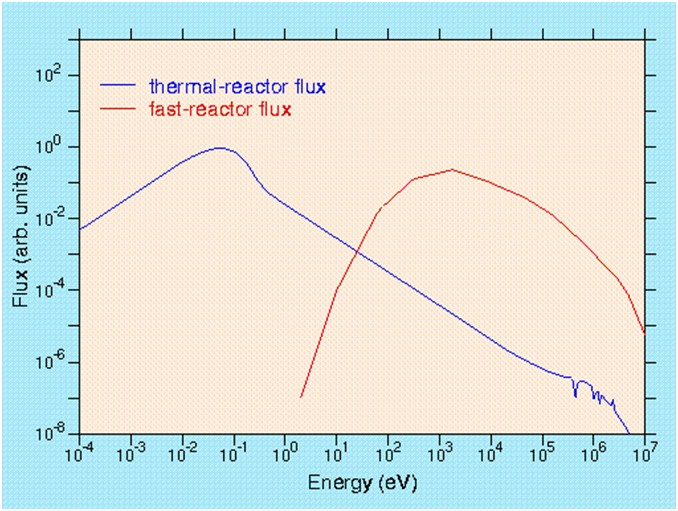
\includegraphics[width=7.0cm]{chapters/introduction/images/reactor-flux.png}
    \caption{Typical Reactor Flux - Thermal and Fast Spectra}
    \label{fig:flux1}
  \end{center}
\end{figure}

Natural U contains 0.7\% ${}^{235}_{92}U$ and 99.3\% ${}^{238}_{92}U$\cite{uraniumenrichment}.  The thermal fission cross section for ${}^{238}_{92}U$ is small for thermal neutrons, and can be measured in the microbarn to millibarn range, but it has a much higher fission cross section with fast neutrons with a cross section closer to 1 barn for neutrons with an energy of 1MeV or more.  The neutron flux in a fast reactor is spread over a higher energy band than that of a thermal neutron reactor (fig. \ref{fig:flux1}).

Fast neutron reactors have been tested and used since the 1950s, and there are several \acrshort{gen4} reactor designs based on this approach.  Given the much larger percentage of ${}^{238}_{92}U$ in natural U, Fast Neutron Reactors have a larger stockpile of fuel.  They also breed fissile isotopes, ${}^{239}_{94}Pu$ and ${}^{241}_{94}Pu$.  This has its advantages and disadvantages.  The advantage is clear, as it produces fissile fuel as it runs, but the creation of fissile materials is a concern as these isotopes could be used in nuclear weapons.

\subsubsection{Lead-cooled Fast Reactors}

Light elements such as the hydrogen in water molecules, or carbon in a graphite stack, allow neutrons to efficiently lose energy.  When neutrons scatter inelastically with heavier elements, such as lead, they lose a much smaller percentage of their energy (figure \ref{fig:inelasticscattering}).

The \acrfull{lfr} uses lead as the coolant.  Lead has a low reaction cross section and, because of its mass relative to a neutron, the kinetic energy lost in collisions is low, keeping more neutrons in the fast energy group.  As the coolant is a liquid, and the boiling point of lead is over $1,970K$, the system will run at atmospheric pressures and any problems associated with void formation due to boiling is removed.  The molten lead will act as a gamma shield and it will be chemically less reactive than the coolant in a \acrfull{sfr} or \acrfull{scwr}.

There are several disadvantages to using lead as a coolant.  The melting point of lead is $600K$, so the reactor would need to be heated first for the coolant to become a liquid.  This also restricts the lowest temperature and thus the maximum efficiency possible that may be extracted from the system without the coolant forming a solid.  The density of lead also poses a problem for the structure needed to support the reactor.

\begin{figure}[htbp]
  \begin{center}
    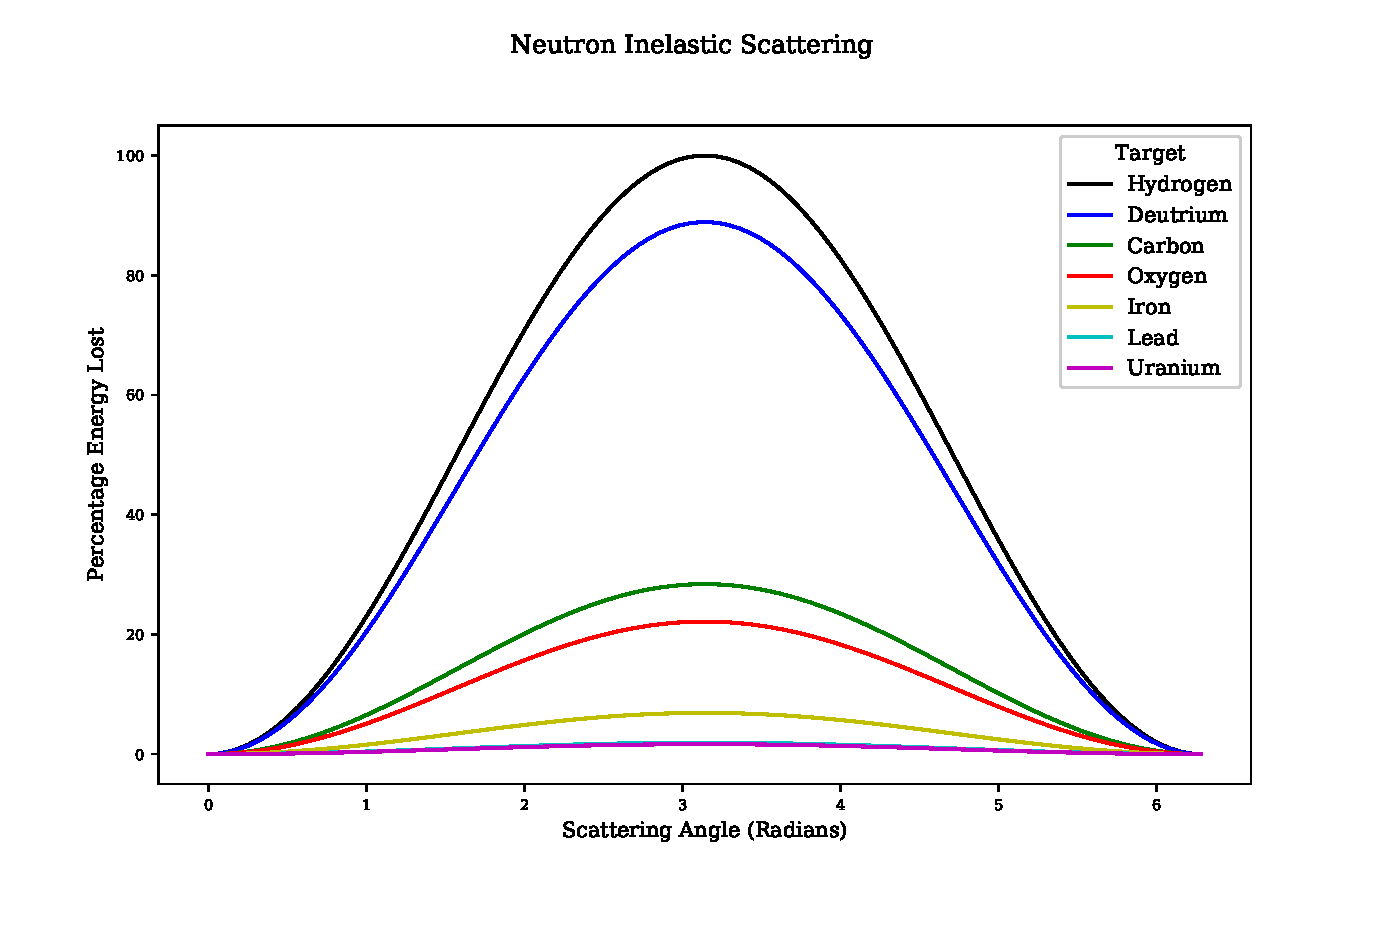
\includegraphics[width=7.0cm]{chapters/introduction/plots/neutron_scattering/neutron_scattering.eps}
    \caption{Inelastic scattering - scattering angle vs energy loss for a range of target atoms}
    \label{fig:inelasticscattering}
  \end{center}
\end{figure}

\acrfull{elsy} is a 600MWe Lead-Bismuth \gls{eutectic} cooled fast neutron reactor.  It has a lower melting point than lead, but there are concerns for the transmutation of Bismuth to Polonium.  The 9,000 tonne molten lead coolant and the high flux of fast neutrons\cite{lanltour} will be challenging conditions to overcome.



\FloatBarrier
\subsubsection{\acrshort{vhtr}}

Traditional nuclear power plants, as well as coal and the secondary cycle of \acrshort{ccgt} plants, boil water to drive turbines.  \acrfull{vhtr} designs use thermal neutrons and a fissile fuels.  Designs plan to have outlet temperatures of up to $1,270K$\cite{genivgifvhtr}.  With a helium coolant, there are several options.

\begin{itemize}
\item directly drive turbines
\item heat water to create steam and drive turbines
\item use the high temperature to help create hydrogen, and combine with steam driven turbine
\end{itemize}

Hydrogen may be extracted from high temperature water either by a thermo-chemical, high temperature electrolysis or a hybrid process\cite{hydrogenhtr}.  Each process benefits from the very high temperatures provided by the predicted outlet temperatures (fig \ref{fig:energyhydrogenproduction}).

\begin{figure}[tbp]
  \begin{center}
    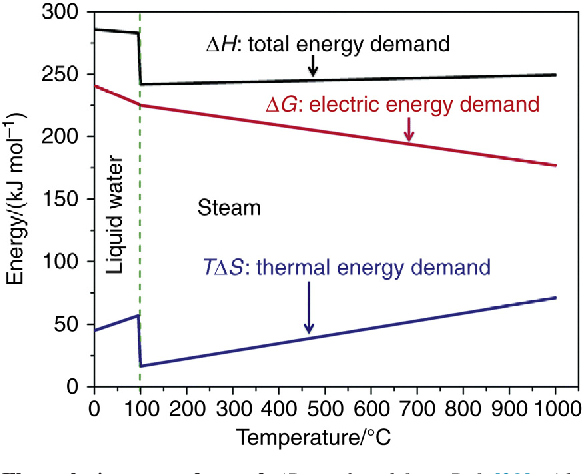
\includegraphics[width=7.0cm]{chapters/introduction/images/hydrogen-from-water.png}
    \caption{Energy demand to produce hydrogen by electrolysis as temperature changes}
    \label{fig:energyhydrogenproduction}
  \end{center}
\end{figure}

The \acrfull{pbr} is a type of \acrshort{vhtr} where spherical fuel pellets are held in a hopper shaped reactor.  Temperatures within the core may reach $1,770K$, and this will pose a challenge for materials scientists.

\FloatBarrier
\subsubsection{\acrshort{gfr}}

The \acrfull{gfr} design is similar to the \acrshort{vhtr}, but rather than use thermal neutrons, it will use fast neutrons.  The design will use a ceramic core and have outlet temperatures up to $1120K$.  This will give similar options to the \acrshort{vhtr} where high temperatures would be used to assist in the production of hydrogen, or it would be used to power a turbine with a secondary steam powered circuit similar to that of a \acrshort{ccgt}.

There are challenges ahead, including the development and testing of advanced materials that can withstand these temperatures while under high energy neutron flux.  However, unlike \acrshort{lfr}s, \acrshort{sfr}s and \acrshort{scwr}s, the coolant is chemically inert and isn't transmuted by neutrons removing the risk of the coolant becoming radioactive.


\FloatBarrier
\subsubsection{\acrshort{sfr}}

Memories of small amounts of sodium, kept under oil in school chemistry labs, being carefully cut and prepared ahead of a violent reaction with water, probably come to mind at the first mention of an \acrfull{sfr}.  It may not be the first choice of an element to use as a coolant, but it does have advantages.  In fact Admiral Rickover once remarked \enquote{if the oceans were filled with liquid sodium, then some crazy scientist would want to build a water-cooled reactor} when the idea of a sodium cooled reactor in a submarine was proposed\cite{atomicaccidents}.

Sodium has a low melting point, of just under $370K$, and a boiling point of $1,150K$.  With an operating temperature of up to $820K$, the reactor would be able to run at atmospheric pressure and without the issues associated with the coolant boiling.  The density of Na is $0.971 gcm^{-3}$ and comparing this to the \acrshort{lfr} the coolant would be 12 times less dense and this would have advantages when designing the structure.

There have been several \acrshort{sfr}s built and operated using this technology, such as the Russian BN-600 reactor.  This particular reactor has a sodium primary loop which heats a secondary sodium loop which in turn heats a third loop for water and steam.




\subsubsection{\acrshort{scwr}}

At 647K and a pressure of 22.1MPa (approximately 218 atmospheres), water becomes \gls{supercritical} (fig. \ref{fig:waterphasespressuretemp}) and at this point it is neither a liquid or a gas\cite{advancedbiomass}.  The current generation \acrshort{pwr} and \acrshort{bwr} operate at approximately $501-598K$ at 15.2MPa\cite{ocw01} and $551-560K$ at 7.1MPa\cite{ocw02} respectively.

\begin{figure}[tbp]
  \begin{center}
    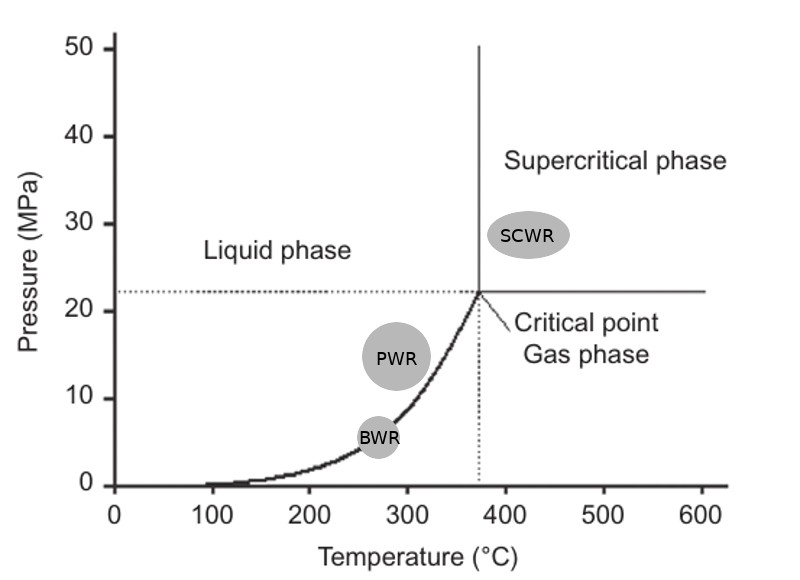
\includegraphics[width=7.0cm]{chapters/introduction/images/water_phase_diagram.png}
    \caption{Phases of Water:  Pressure vs Temperature}
    \label{fig:waterphasespressuretemp}
  \end{center}
\end{figure}

Supercritical water exists above $647K$ and 22.1MPa, and in this state water has a higher thermodynamic efficiency.  The design of the nuclear power plant is also simplified as there is no phase change of the water, so a condenser is not needed.  The \acrfull{scwr} is the only \acrshort{gen4} reactor design that uses water as the coolant\cite{gen4}.  The economic benefits have already been seen in SCW fossil fuel power stations, and it is incorporated in \acrshort{gen4} water cooled fast and thermal reactors.  

There are side effects to using supercritical water.  It is an oxidant and is now being considered to \enquote{burn} organic waste in future waste processing plants.  The combination of supercritical water chemistry and irradiation damage must be considered, as well as higher temperature and pressure, when considering the materials used by a \acrshort{scwr}.




\FloatBarrier
\subsubsection{\acrlong{msr}}

\acrshort{msr}s have been operated for over 50 years.  Chemically, salts are very stable, and this has obvious safety benefits over reactors like the \acrshort{sfr}.  The coolants are fluoride salts that have high boiling points which gives the added safety protection of being able to operate at atmospheric pressure, unlike a \acrshort{pwr} where a pressure vessel is needed.

The fuel is dissolved into the molten salt.  There are no solid fuel rods to place into the core, remove or reprocess.  The molten salt is processed on the site to remove poisons, waste and add new fuel.  

\acrshort{msr}s may use either thermal or fast neutrons and a range of fuels including \Gls{Th}.  This is particularly interesting as Th is three times as abundant as U and would increase the fuel available to us for the clean production of electricity by nuclear power.

A safety feature that takes advantage of the fuel being dissolved in the molten salt are large drain tanks under the reactor.  A plug is designed to melt if it reaches a certain temperature and this would quickly drain the molten salt from the reactor into large and cold drainage tanks.  The reactivity would drop and the fuel would cool reverting it to a solid salt. 

Salts considered in various designs are chlorides, nitrates and fluorides.  Corrosion of the reactor due to the molten salts is a concern.  Elements that provide protection to corrosion, such as Cr, are prone to dissolution into the molten salt\cite{msrcorrosion}.  Where the fuel is suspended in the molten salt as \acrfull{triso} fuel particles, formation of chromium-carbide precipitates may be an issue.


\FloatBarrier
\subsubsection{Experimental Fusion Reactors}

Nuclear Fusion is a very attractive technology and could be the answer to all of our energy problems.  Much work is being invested in developing this technology and the \acrfull{iter} has been designed to output more energy than is required to start the fusion reaction.  The process of fusion combines two isotopes of hydrogen and creating helium, fast neutrons (eq. \ref{eq:fusionreaction}) and an excess of energy.  As neutrons have no charge, they can penetrate shielding causing damage as they lose energy through nuclear interactions.   Any atoms they interact with have a chance to capture the neutron and become unstable.

\begin{equation}
_{1}D^{2} + _{1}T^{3} \to _{2}He^{4} (3.5MeV) + _{0}n^{2} (14.1MeV)
\label{eq:fusionreaction}
\end{equation}

The fast neutron spectrum for fission reactors ranges from a few eV to a few MeV, whereas the neutrons in a fusion reaction have 2-3 times more energy than the most energetic neutrons from fast fission.  Engineers must develop materials to construct components that will be resilient to this damage, while having a low reaction cross section and being able to withstand other extreme conditions within the reactor.  

Unfortunately, nuclear fusion as a commercial method of creating energy, is often said to be 30 years away, and this has been the case for some time now.  It is a lot to ask, recreating a process that occurs within a star, in a safe and steady manner.  Once this problem is solved, it could mark a turning point for human civilization.




%%%%%%%%%%%%%%%%%%%%%%%%%%%%%%%%%%%%%%%%%%%%%%%%%%%%%%%%%%%%%%%%%%%%%%%%%%%%%%%%%%%%%%%%%%%%%%%%%%%%%%%%%%
%%
%%  REACTION AND NEUTRON SPECTRA
%%  
%%%%%%%%%%%%%%%%%%%%%%%%%%%%%%%%%%%%%%%%%%%%%%%%%%%%%%%%%%%%%%%%%%%%%%%%%%%%%%%%%%%%%%%%%%%%%%%%%%%%%%%%%%


\FloatBarrier
\section{Damage to Nuclear Core Components by Neutrons}

Radiation damage in a reactor is caused by several projectiles.  Fission fragments are heavy, contain charged particles and lose energy close to their source.  Gamma rays excite electrons, promoting them to higher energy levels, or ionise the atoms where there is enough energy to eject electrons completely from atoms.  They do not have the momentum to knock atoms out of place.  Fast neutrons, however, may impart a great deal of momentum to a target atom and, as they are neutral, travel much further into a material than fission fragments.  With enough energy, neutrons cause large damage cascades within the material.

One fuel source for many of the \acrshort{gen3+} and \acrshort{gen4} reactors is ${}^{235}_{92}U$, whether as enriched U or otherwise.  The neutron(s) released by the fission of ${}^{235}_{92}U$ atoms have a spectra of energy (fig. \ref{fig:neutronfissionspectra}) which may roughly be split into four categories: cold (below 0.025eV), thermal (0.025eV), slow and intermediate (above 0.025eV and below 1MeV) and fast (1MeV and above).

\begin{figure}[htbp]
  \begin{center}
    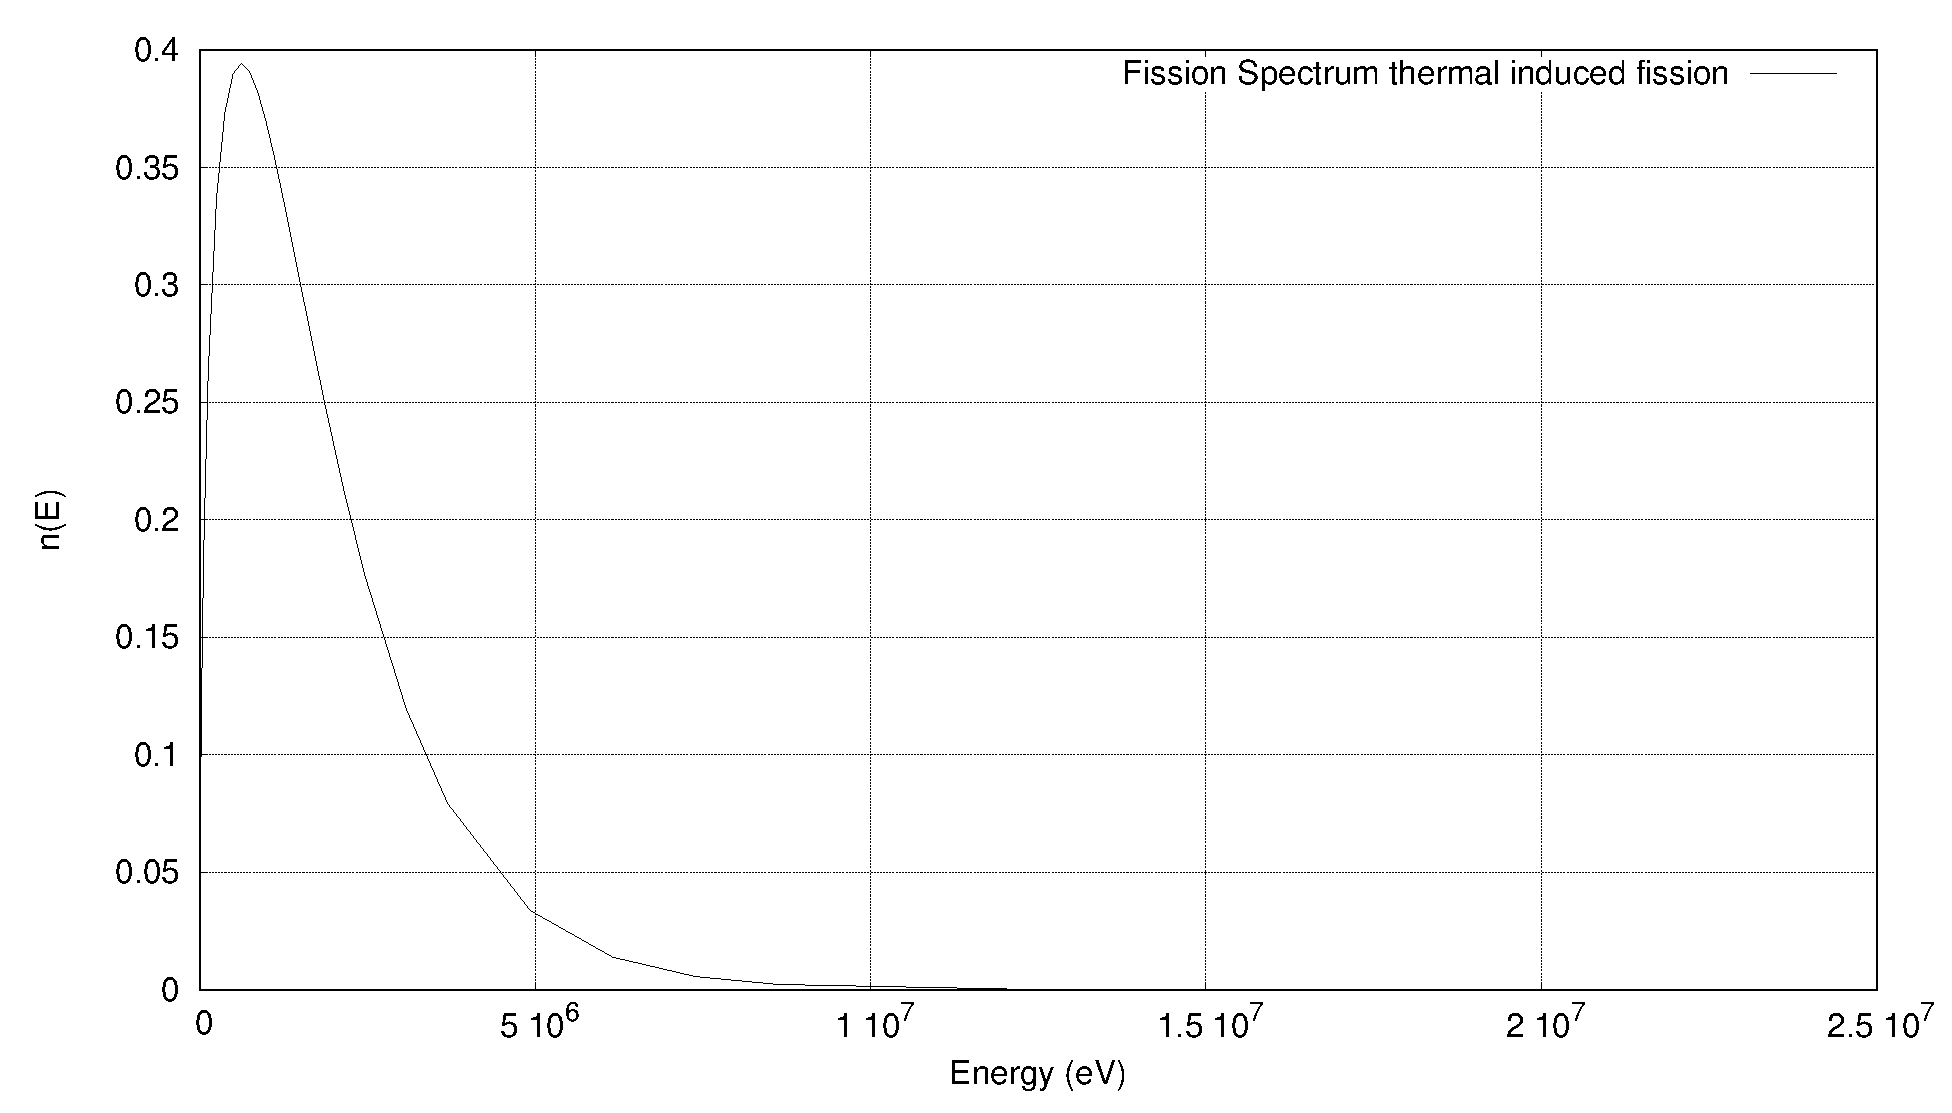
\includegraphics[width=10.0cm]{chapters/introduction/plots/fission_spectra/fission_spectra.eps}
    \captionsetup{font={it}}
    \caption{Neutron Energy Spectrum from Fission\cite{jeff311}}
    \label{fig:neutronfissionspectra}
  \end{center}
\end{figure}

Thermal and slow/intermediate neutrons cause damage in their own particular way, as they are captured by and transmute the atoms within the target material.  Fast neutrons have enough energy to create a great deal of damage, whereby they transfer kinetic energy to an atom in the material that become the \acrfull{pka} in a cascade of atoms through the material.  Neutrons can travel deep into a material, creating many damage cascades through the material until they lose enough  energy or pass through the material completely.

\begin{figure}[htbp]
  \begin{center}
    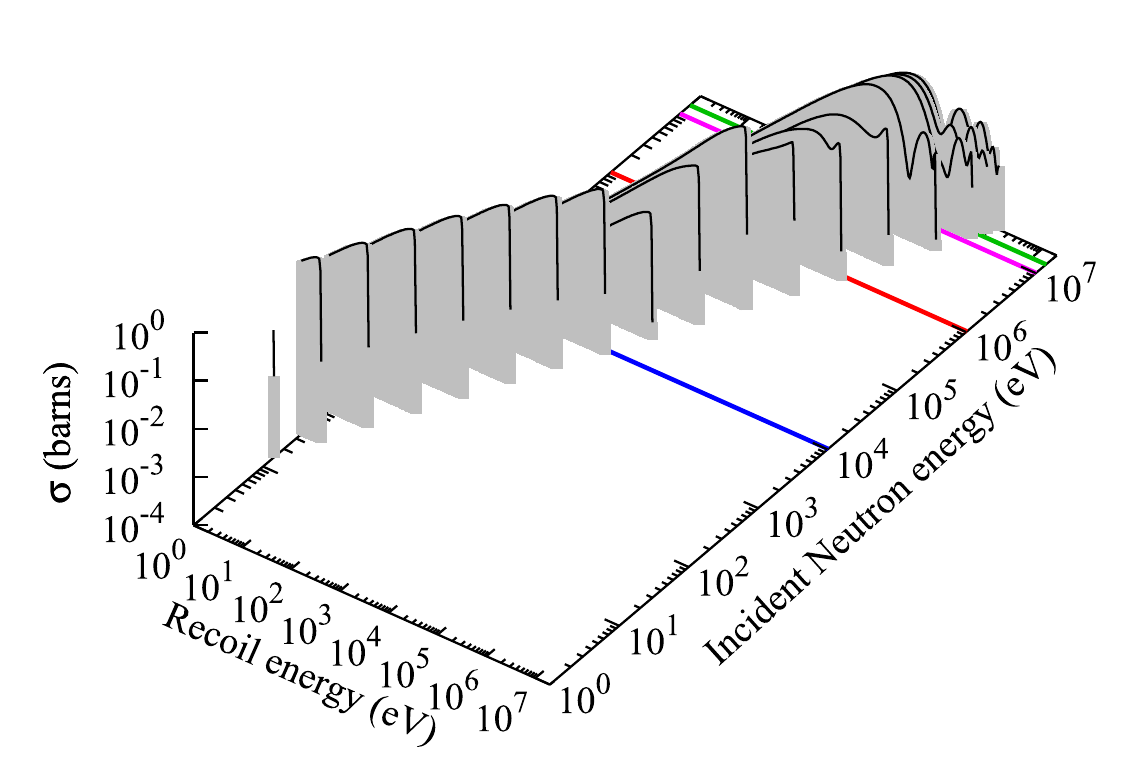
\includegraphics[width=10.0cm]{chapters/introduction/plots/damage/pkaenergy.png}
    \captionsetup{font={it}}
    \caption{\acrshort{pka} energy as a funtion of neutron energy in Fe\cite{pkaenergyspectra}}
    \label{fig:neutronironrecoil}
  \end{center}
\end{figure}

The intensity of neutron energies from the fission of ${}^{235}_{92}U$ peaks around 1MeV (fig. \ref{fig:neutronfissionspectra}).  The energy transferred to \acrshort{pka}s will vary depending on the mass of the target nucleus and scattering angle but, in Fe at least, 1MeV neutrons will create the majority of its Fe \acrshort{pka}s with energies ranging from 1keV to 100keV (fig. \ref{fig:neutronironrecoil}).




%%%%%%%%%%%%%%%%%%%%%%%%%%%%%%%%%%%%%%%%%%%%%%%%%%%%%%%%%%%%%%%%%%%%%%%%%%%%%%%%%%%%%%%%%%%%%%%%%%%%%%%%%%
%%
%%  Ion Irradiation
%%  
%%%%%%%%%%%%%%%%%%%%%%%%%%%%%%%%%%%%%%%%%%%%%%%%%%%%%%%%%%%%%%%%%%%%%%%%%%%%%%%%%%%%%%%%%%%%%%%%%%%%%%%%%%




\FloatBarrier
\section{Radiation Damage: Replacing Neutrons with Protons}

It is difficult to generate large fluxes of neutrons.  When we pick up a cup, press keys on a keyboard, they react because of the electromagnetic force.  Neutrons have no net charge, so they cannot be controlled in a similar way.  Nuclear reactors are the most common way to create large fluxes of neutrons.

This an expensive method, and one that make be inconvenient as the sample being tested would need to be placed inside a reactor.  Rather than do this, ions may be used to replicate the damage cause by neutrons, but in a more controlled and accessible way.

A major side effect from the process of nuclear fission is the creation of both radioactive fission fragments and radioactive isotopes within the components and structural material of the reactor.  Low energy protons are not captured as low energy neutrons would be, due to the opposing electromagnetic force between the proton and nucleus of the target atom.  Once the proton energies exceed a few MeV, they have sufficient energy to transmute target nuclei.

By virtue of detailed reaction cross section data files and decay data, the amount of radioactivity induced by both protons and neutrons may be calculated.  This will assist in the selection of proton beam parameters to replicate irradiation damage, to the required \acrshort{dpa}, whilst keeping the radioactivity at a safe level.


%%%%%%%%%%%%%%%%%%%%%%%%%%%%%%%%%%%%%%%%%%%%%%%%%%%%%%%%%%%%%%%%%%%%%%%%%%%%%%%%%%%%%%%%%%%%%%%%%%%%%%%%%%
%%
%%  Molecular Dynamics
%%  
%%%%%%%%%%%%%%%%%%%%%%%%%%%%%%%%%%%%%%%%%%%%%%%%%%%%%%%%%%%%%%%%%%%%%%%%%%%%%%%%%%%%%%%%%%%%%%%%%%%%%%%%%%


\FloatBarrier
\section{Simulation Material Damage}

Irradiating and testing materials irradiated by both neutrons and protons have a number of drawbacks, including expensive facilities and the creation of radioactive waste.  Simulations may be used to help understand the processes on a mesoscopic scale and make predictions on how the material in question may behave inside a reactor under certain specified conditions.

Part of this work focuses on the damage of stainless steel by neutrons.  The damage process occurs on time scales and sizes too small to capture experimentally and play back to study.  The theories may not be sufficiently well understood, or are often unsolvable with current techniques.  Modelling helps bridge the gap between theory and experiment. 

\subsection{Molecular Dynamics}
 
Molecular dynamics models have been used to simulate radiation damage.  Damage cascades caused by \acrfull{pka}s with energies of 10, 20 and 50KeV have been modelled in \acrshort{bcc} \Gls{W}\cite{damagebcctungsten}, whilst cascades caused by \acrshort{pka}s of 5, 10 and 20KeV have been simulated in \acrshort{bcc} Fe\cite{damagebcciron}.

Neutrons have a long mean path before interacting with a target when compared to ions.  It would be impossible with current and foreseable technology to simulate a neutron travelling through a material because the volume of the material, and the number of atoms and interactions between atoms, would be so large.  Rather than attempt this, it is more productive to focus on individual damage cascades caused by \acrshort{pka}s in order to conserve computing resources.

\begin{figure}
\begin{subfigure}{.5\textwidth}
  \centering
  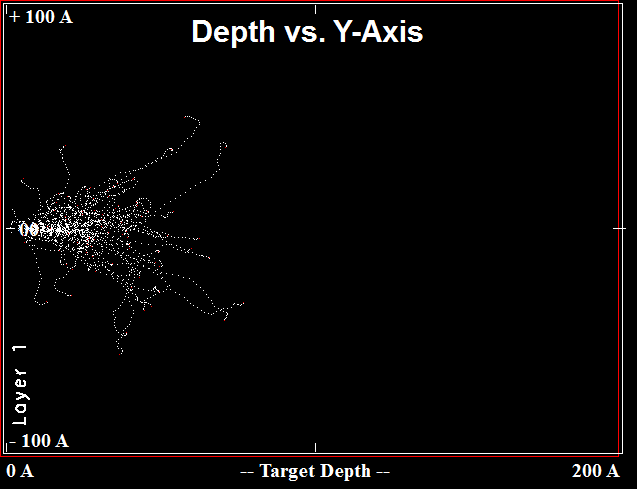
\includegraphics[width=.7\linewidth]{chapters/introduction/images/5KeV.png}
  \caption{} \label{fig:damagecascade5kev}
\end{subfigure}
\begin{subfigure}{.5\textwidth}
  \centering
  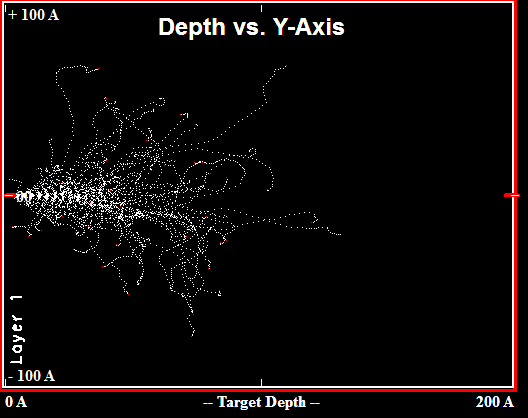
\includegraphics[width=.7\linewidth]{chapters/introduction/images/10KeV.png}
  \caption{} \label{fig:damagecascade10kev}
\end{subfigure}
\begin{subfigure}{.5\textwidth}
  \centering
  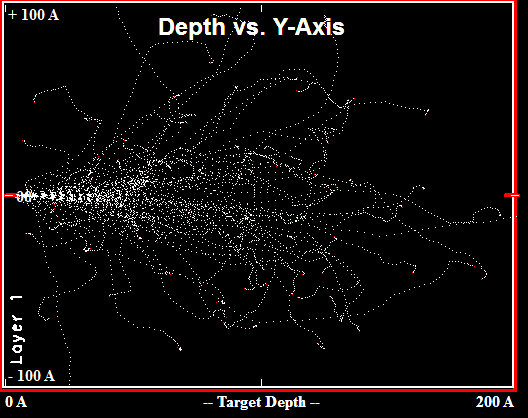
\includegraphics[width=.7\linewidth]{chapters/introduction/images/20KeV.png}
  \caption{} \label{fig:damagecascade5kev}
\end{subfigure}
\begin{subfigure}{.5\textwidth}
  \centering
  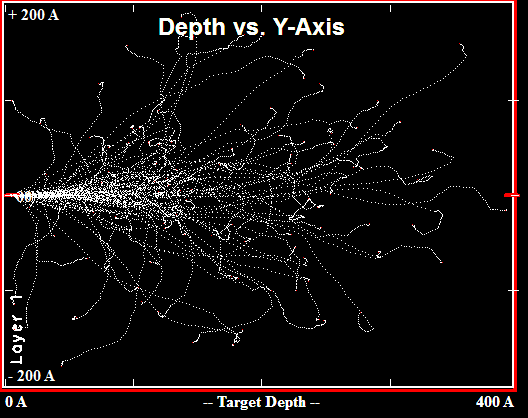
\includegraphics[width=.7\linewidth]{chapters/introduction/images/50KeV.png}
  \caption{} \label{fig:damagecascade10kev}
\end{subfigure}
\captionof{figure}{(a) 5KeV Fe PKA Damage Cascade in Fe (b) 10KeV Fe PKA Damage Cascade in Fe (c) 20KeV Fe PKA Damage Cascade in Fe (d) 50KeV Fe PKA Damage Cascade in Fe}
\label{fig:damagecascades}
\end{figure}


\FloatBarrier

Molecular Dynamics simulations require interatomic potentials to govern how the atoms in the simulation interact with one another.  Typical simulation sizes range from thousands of atoms to millions of atoms.

Fe has a density of approximately $8.5 \times 10^{-2}$ atoms per cubic angstrom, and this leads to simulation sizes between almost one million atoms and fifty million atoms for cascades with \acrshort{pka}s ranging from 5KeV to 50KeV (fig \ref{fig:damagecascades}, table \ref{table:fesimulationsize}).

\begin{table}[h]
\begin{center}
\renewcommand{\arraystretch}{1.2}
\begin{tabular}{c c c}
\hline\hline
PKA Energy (KeV) & Volume $(Ang^3)$ & Atoms \\
\hline\hline
5 & $1.0\times 10^6$ & $9.0\times 10^5$ \\
10 & $6.0\times 10^6$ & $5.4\times 10^6$ \\
20 & $8.0\times 10^6$ & $6.9\times 10^6$ \\
50 & $6.4\times 10^7$ & $5.5\times 10^7$ \\
\hline\hline
\end{tabular}
\end{center}
\caption{Approximate simulation sizes by PKA energy}
\label{table:fesimulationsize}
\end{table}

The interatomic potentials used to simulate a damage cascade must be able to model the very close separations during the collisions event.  For very close separations, an exponential potential such as the \acrfull{zbl} potential may be used, and for other separations a standard potential such as the \acrfull{eam} may be used, in particular for metals.

There have been attempts to create potentials based on Physics, but the nuances are still poorly understood and there aren't any models that can be applied accurately to any material type under any set of circumstances.  A number of recent interatomic potentials, including a selection of transition metals, have been fit to match the experimental data rather than the underlying physics.


\FloatBarrier
\subsection{Density Functional Theory}

In quantum mechanics, the Schr\"{o}dinger equation and the wavefunction of a system describes all that can be known about that quantum system.  Unfortunately, it is very difficult to compute when there are just several electrons in the system.  Many atoms in a system makes this an impossible task with current technology.

\acrfull{dft} replaces the many electron wavefunction with a single electron wavefunction.  Rather that use the positions of all the electrons, which would result in $3^n$ parameters, the charge density, which varies in space with just 3 parameters, is used.

\acrshort{dft} allows for the calculation of the forces between atoms and the energy of that collection of atoms by replacing the many parameters to give the coordinates of many electrons with the three coordinates for the charge density.  From the forces the optimum (relaxed) basis vector and atom positions may be computed, and from the energy of multiple configurations other properties are computable (bulk modulus, elastic constants, etc).

It is important to note that \acrshort{dft} is an exact method for ground state calculations, although in practice approximations do need to be made in order to solve problems.


\subsection{Interatomic Potentials for Molecular Dynamics}

Interatomic potentials help to describe the interaction between atoms.  Originally they were used for pairs of atoms and a collection of atoms on a pair by pair basis, but in the 1980s the complexity of potentials increased as they started to include the effects of the background electron density that the atoms are embedded in.  This lead to the \acrfull{fs} and \acrfull{eam} type potentials.

Whilst \acrshort{dft} is a purer form of computational materials science, more closely linked to physics, it is computationally intensive and suitable for small systems of hundreds to thousands of atoms.  By using interatomic potentials to recreate the forces and energies that would be computed by \acrshort{dft}, the systems may be increased in size to thousands to millions of atoms, and these calculations may be run over a time frame with hundreds or thousands of time steps.

There are a wide range of potentials, and these are typically selected based on the type of material and the required accuracy.  Simple pair potentials may still be used, but angularly dependent potentials have been developed for materials with covalent bonds, and metals use \acrshort{fs} and \acrshort{eam} potentials.  The potentials are made up of a set of functions, and these functions change from derivation to derivation.  




%%%%%%%%%%%%%%%%%%%%%%%%%%%%%%%%%%%%%%%%%%%%%%%%%%%%%%%%%%%%%%%%%%%%%%%%%%%%%%%%%%%%%%%%%%%%%%%%%%%%%%%%%%
%%
%%  Scope and Objectives
%%  
%%%%%%%%%%%%%%%%%%%%%%%%%%%%%%%%%%%%%%%%%%%%%%%%%%%%%%%%%%%%%%%%%%%%%%%%%%%%%%%%%%%%%%%%%%%%%%%%%%%%%%%%%%

%%\section{Scope and Objectives}





%%##################################################################
%% Background
%%##################################################################

\chapter{Consequences of Ionizing Radiation}
\label{chap:backgroundsources}

\begin{changemargin}{1.0cm}{1.0cm}
\abstractpreamble{Ionizing radiation takes on a number of forms and may be damaging to both materials and organic life.  The various radiations interact differently with matter and cause damage in different ways.\\
\\
Radiation may interact directly with matter.  In the case of materials this could mean creating a damage cascade that displaces atoms from their lattice sites.  For organic life, this might mean the damage of strands of \acrshort{dna} leading to the death of a cell or problems when the cell tries to replicate.  Radiation may also change the environment and an example of this is the radiolysis of water.  This change in water chemistry can affect both materials and organic life.\\
\\
The amount of damage components in a reactor must withstand are measured in terms of displacements per atom.  Dose to organic life, in particular humans, is measured in a variety of units including Gy, Si and REM.  Determining the amount of dose in each case can be a complicated process, but it is needed to ensure safety of workers and correct testing of materials.}
\end{changemargin}



%%%%%%%%%%%%%%%%%%%%%%%%%%%%%%%%%%%%%%%%%%%%%%%%%%%%%%%%%%%%%%%%%%%%%%%%%%%%%%%%%%%%%%%%%%%%%%%%%%%%%%%%%%
%%
%%  RADIATION TYPES
%%
%%%%%%%%%%%%%%%%%%%%%%%%%%%%%%%%%%%%%%%%%%%%%%%%%%%%%%%%%%%%%%%%%%%%%%%%%%%%%%%%%%%%%%%%%%%%%%%%%%%%%%%%%%


\section{Radiation Types Relevant to This Work}


\subsection{Introduction}

There are three types of radiation that are useful to discuss in this work: neutrons, ions and gammas, and two of these (neutrons and protons) are of particular interest in this work.  Each of these are capable of ionizing the atoms they interact with, given sufficient energy.  Higher energy and momentum radiation it is able to directly damage materials or the \acrshort{dna} structure of organic life that it interacts with.  Lower momentum ionizing radiation may change the water chemistry of the environment or within the cells of organic lifeforms that is detrimental to life.



\subsection{Protons and other Ions}

Charged particles interact with matter through the Coulomb interaction.  As a charged particle passes through matter, it may interact with both the nucleus and electrons of an atom.  A sufficiently energetic ion may lose kinetic energy to electrons by either raising the electrons to higher energy levels in their atoms, or by removing electrons from atoms altogether, causing the ionization of those atoms.  

Ions may also lose kinetic energy to the nucleus of an atom through elastic scattering and, where the atom is in a crystal structure, through knocking atoms in the material out of their lattice positions.  Inelastic scattering is also a possibility, leaving the target nucleus in an excited state.

Knock on atoms and electrons with enough kinetic energy that have been removed from atoms (delta rays), continue the irradiation of the material whilst they have the kinetic energy available to do so.

A large proportion of the energy of a charged projectile is lost to the electrons of the target material.  There is a chance, depending on the energy and type of charged projectile (and the cross section of the target nucleus), that the charged particle will overcome the coulomb potential and be captured by the nucleus.

This may result in a stable nucleus or an unstable nucleus.  If it is unstable, there is a probability that it will decay releasing energy in the form of photons, nucleons or electrons.  The initial ion irradiation creates sources of further radiation within the target material.



\FloatBarrier
\subsection{Neutrons}


Neutrons interact with matter differently to that of protons, ions and other atoms, as the neutron has no overall charge.  Neutrons do have a magnetic moment and experience a weak interaction with unpaired electrons by a dipole-dipole interaction.  Neutrons also interact with the nucleus of atoms, and this is dependant upon the target atom and the energy of the projectile neutron.  The energy of neutrons may be grouped as shown in table \ref{table:neutronenergies}, and as mentioned earlier, thermal neutrons are of interest to current reactor designs, and fast neutrons are of interest to several future designs.
 
\begin{table}[h]
\begin{center}
\renewcommand{\arraystretch}{1.2}
\begin{tabular}{c c c c}
\hline\hline
Name & Energy Range & Velocity/ms\textsuperscript{-1} & Wavelength Ang \\
\hline\hline
Cold & 0-0.025 eV & 0.0 - $2.2 \times 10^{3}$ &  $> 1.8$  \\
Thermal & 0.025 eV & ~$2.2 \times 10^{3}$ &  1.8  \\
Epithermal & 0.025-0.4 eV & $2.2 \times 10^{3}$ - $8.8 \times 10^{3}$ &  0.5-1.8 \\
Cadmium & 0.4-0.6 eV & $8.8 \times 10^{3}$ - $1.1 \times 10^4$ & 0.4-0.5  \\
Epicadmium & 0.6-1.0 eV & $1.1 \times 10^4$ - $1.4 \times 10^4$ & 0.3-0.4\\
Slow & 1-10 eV & $1.4 \times 10^4$ - $4.4 \times 10^4$   & 0.09-0.3\\
Resonance & 10-300 eV & $4.4 \times 10^4$ - $2.4 \times 10^5$ & 0.02-0.09\\
Intermediate & 300 eV - 1 MeV &  $2.4 \times 10^5$ & $2.9 \times 10^{-4}$ - $0.02$\\
Fast & 1-20 MeV & $1.4 \times 10^7$ - $6.1 \times 10^7$ & $6.5 \times 10^{-5}$ - $2.9 \times 10^{-4}$ \\
Relativistic & $>20$ MeV & $>6.1 \times 10^{7}$ & $< 6.5 \times 10^{-5}$\\
\hline\hline
\end{tabular}
\end{center}
\caption{Neutron Categories by Energy Range \cite{njcarron}}
\label{table:neutronenergies}
\end{table}

The nuclear force holds nuclei together by exchanging pions and the types of interactions are shown in figure \ref{fig:pninteractions}.  It is 137 times stronger than the electromagnetic force, but because of the mass of the pion (approximately 130-140MeV) it only acts over a short range of approximately 1fm.  The nuclear force is attractive but has a short-range repulsive core.

\begin{figure}[htb]
\centering
\begin{subfigure}{0.32\textwidth}
\begin{tikzpicture}
  \begin{feynman}
    \vertex (a) {\(p\)};
    \vertex [below right=of a] (b);
    \vertex [above right=of b] (c) {\(p\)};
    \vertex [below right=of b] (d);
    \vertex [below left=of d] (f) {\(p\)};
    \vertex [below right=of d] (g) {\(p\)};
    \diagram* {
      (a) -- [fermion] (b),
      (b) -- [fermion] (c),
      (b) -- [scalar, edge label=\(\Pi^{0}\)] (d),
      (f) -- [fermion] (d),
      (d) -- [fermion] (g),
    };
  \end{feynman}
\end{tikzpicture}
\caption{Direct interaction p-p\cite{pionexchange}}
\label{fig:pppion}
\end{subfigure}
\begin{subfigure}{.32\textwidth}
\begin{tikzpicture}
  \begin{feynman}
    \vertex (a) {\(p\)};
    \vertex [below right=of a] (b);
    \vertex [above right=of b] (c) {\(p\)};
    \vertex [below right=of b] (d);
    \vertex [below left=of d] (f) {\(n\)};
    \vertex [below right=of d] (g) {\(n\)};
    \diagram* {
      (a) -- [fermion] (b),
      (b) -- [fermion] (c),
      (b) -- [scalar, edge label=\(\Pi^{0}\)] (d),
      (f) -- [fermion] (d),
      (d) -- [fermion] (g),
    };
  \end{feynman}
\end{tikzpicture}
\caption{Direct interaction p-n\cite{pionexchange}}
\label{fig:pnpion}
\end{subfigure}
\begin{subfigure}{.32\textwidth}
\begin{tikzpicture}
  \begin{feynman}
    \vertex (a) {\(n\)};
    \vertex [below right=of a] (b);
    \vertex [above right=of b] (c) {\(n\)};
    \vertex [below right=of b] (d);
    \vertex [below left=of d] (f) {\(n\)};
    \vertex [below right=of d] (g) {\(n\)};
    \diagram* {
      (a) -- [fermion] (b),
      (b) -- [fermion] (c),
      (b) -- [scalar, edge label=\(\Pi^{0}\)] (d),
      (f) -- [fermion] (d),
      (d) -- [fermion] (g),
    };
  \end{feynman}
\end{tikzpicture}
\caption{Direct interaction n-n\cite{pionexchange}}
\label{fig:nnpion}
\end{subfigure}

\begin{subfigure}{.32\textwidth}
\centering
\begin{tikzpicture}
  \begin{feynman}
    \vertex (a) {\(p\)};
    \vertex [below right=of a] (b);
    \vertex [above right=of b] (c) {\(n\)};
    \vertex [below right=of b] (d);
    \vertex [below left=of d] (f) {\(n\)};
    \vertex [below right=of d] (g) {\(p\)};
    \diagram* {
      (a) -- [fermion] (b),
      (b) -- [fermion] (c),
      (b) -- [scalar, edge label=\(\Pi^{+}\)] (d),
      (f) -- [fermion] (d),
      (d) -- [fermion] (g),
    };
  \end{feynman}
\end{tikzpicture}
\caption{Exchange interaction n-p\cite{pionexchange}}
\label{fig:pppion}
\end{subfigure}
\begin{subfigure}{.32\textwidth}
\centering
\begin{tikzpicture}
  \begin{feynman}
    \vertex (a) {\(n\)};
    \vertex [below right=of a] (b);
    \vertex [above right=of b] (c) {\(p\)};
    \vertex [below right=of b] (d);
    \vertex [below left=of d] (f) {\(p\)};
    \vertex [below right=of d] (g) {\(n\)};
    \diagram* {
      (a) -- [fermion] (b),
      (b) -- [fermion] (c),
      (b) -- [scalar, edge label=\(\Pi^{-}\)] (d),
      (f) -- [fermion] (d),
      (d) -- [fermion] (g),
    };
  \end{feynman}
\end{tikzpicture}
\caption{Exchange interaction p-n\cite{pionexchange}}
\label{fig:pnpion}
\end{subfigure}
\caption{Proton and neutron interactions}
\label{fig:pninteractions}
\end{figure}

For nuclear reaction and damage calculations, the interaction of neutrons with matter is represented by a cross section (section \ref{section:nuclearxs}).  Cross sections are used to calculate the probability of a certain interaction occurring and are dependent upon the target nucleus, how much of the material the pass through and the energy of the neutron.

The attenuation of neutron radiation is therefore a complicated process.  A much larger thickness of shielding is required to stop neutrons, or at least bring them to thermal temperatures.  Not only this, but the thermalized neutrons must then be captured.  During this process various isotopes within the attenuating shielding will have been transmuted, possibly into radioactive isotopes.  As a rough estimate if a certain amoint of material will attenuate neutrons to 10\% their original flux, then the same amount of material will reduce the flux further to 1\%.  This is however an over simplification and computer codes such as \acrfull{mcnp} and TART more accurately model the transport of neutrons through materials. 



\FloatBarrier
\subsection{High Energy Photons}

The electromagnetic spectrum classifies photons based on their energy and/or source, but visible light, x-rays, gamma rays and so on are all the same elementary \enquote{particle}.  During the early years of Quantum Mechanics, the relationship between the energy and wavelength of a photon was discovered: the Planck-Einstein relation (eq. \ref{eq:planckeinstein}).

\begin{equation}
\begin{split}
E = h f
\end{split}
\label{eq:planckeinstein}
\end{equation}

\subsubsection{Pair Production}

The energy of photons in the database used for this work ranges from 1keV up to almost 10MeV.  There are several ways high energy photons will interact with the atoms of a target material.  The rest mass of an electron is 511keV.  If the photon energy is greater than 1.02MeV, i.e. there is at least enough energy to create an electron and positron, there is a chance that the photon will create an electron-proton pair.  

\begin{equation}
\begin{split}
h f = (m_e + m_p) c^2 + T_e + T_p
\end{split}
\end{equation}

The creation conserves energy and mass, with excess energy carried away as the kintetic energy of the particle pair.  The charge before the creation is zero, as the photon is neutral, and the charge after is also zero, with the -1 of the electron and +1 of the positron cancelling out.  Angular momentum is also conserved; the photon is a spin 1 Boson and, as electrons and positrons are Leptons they have half integer spin, adding up to 1.  Finally, momentum is not conserved in a vacuum, and this is why pair production occurs in the coulomb field of a nucleus.  The nucleus carries away excess momentum, fulfilling this conservation law (fig. \ref{fig:pairproduction}).

\begin{figure}[h]
\begin{center}
\begin{tikzpicture}
  \begin{feynman}
    \vertex (a) {\(\gamma\)};
    \vertex [right=of a] (b);
    \vertex [above right=of b] (c) {\(e^-\)};
    \vertex [below right=of b] (d);
    \vertex [below right=of d] (e) {\(e^+\)};
    \vertex [below =of d] (f);
    \vertex [below left=of f] (g) {\(Z\)};
    \vertex [below right=of f] (h) {\(Z\)};
    \diagram* {
      (a) -- [boson] (b),
      (b) -- [fermion] (c),
      (b) -- [fermion] (d),
      (d) -- [fermion] (e),
      (d) -- [boson] (f),
      (g) -- [fermion] (f),
      (f) -- [fermion] (h),
    };
  \end{feynman}
\end{tikzpicture}
\end{center}
\caption{Pair production Feynman diagram}
\label{fig:pairproduction}
\end{figure}


\subsubsection{Compton Scattering}

An incident photon with enough energy may interact with the electron of an atom, and if it transfers enough kinetic energy it will eject the electron from the atom (fig. \ref{fig:comptonscattering}).  A lower energy photon is also created that carries away the remainder of the energy, but also linear momentum, as both energy and momentum must be conserved.

\begin{figure}[h]
\begin{center}
\begin{tikzpicture}
  \begin{feynman}
    \vertex (a) {\(\gamma\)};
    \vertex [below right=of a] (b);
    \vertex [right=of b] (c);
    \vertex [below left=of b] (d) {\(e^{-}\)};
    \vertex [above right=of c] (e) {\(\gamma\)};
    \vertex [below right=of c] (f) {\(e^{-}\)};
    \diagram* {
      (a) -- [boson] (b),
      (b) -- [fermion] (c),
      (d) -- [fermion] (b),
      (c) -- [boson] (e),
      (c) -- [fermion] (f),
    };
  \end{feynman}
\end{tikzpicture}
\end{center}
\caption{Compton Scattering Feynman diagram}
\label{fig:comptonscattering}
\end{figure}


\subsubsection{Photoelectric Effect}

Photons of sufficient energy interact with and eject electrons from the surface of a metal (fig. \ref{fig:photoelectric}).  At lower energies, the photons have no effect on the electrons.  Ejected electrons have a maximum kinetic energy equal to the difference between the energy of the interacting photon and the workfunction, $T_{max} = h \nu - \phi$.

\begin{figure}[h]
\begin{center}
\begin{tikzpicture}
  \begin{feynman}
    \vertex (a) {\(\gamma\)};
    \vertex [below right=of a] (b);
    \vertex [right=of b] (c);
    \vertex [below left=of b] (d) {\(Z_{n}^{+},e_{n}^{-}\)};
    \vertex [above right=of c] (e) {\(e_{1}^{-}\)};
    \vertex [below right=of c] (f) {\(Z_{n}^{+},e_{n-1}^{-}\)};
    \diagram* {
      (a) -- [boson] (b),
      (b) -- [fermion] (c),
      (d) -- [fermion] (b),
      (c) -- [fermion] (e),
      (c) -- [fermion] (f),
    };
  \end{feynman}
\end{tikzpicture}
\end{center}
\caption{Photoelectric Effect Feynman diagram}
\label{fig:photoelectric}
\end{figure}



\subsubsection{Coherent Scattering}

Lower energy, non-ionizing photons, have insufficient energy to eject electrons (fig. \ref{fig:coherentscattering}).  Coherent scattering is the interaction in which photons change direction, scattering, without losing energy.  This is also known as Rayleigh scattering.


\begin{figure}[h]
\begin{center}
\begin{tikzpicture}
  \begin{feynman}
    \vertex (a) {\(\gamma\)};
    \vertex [below right=of a] (b);
    \vertex [right=of b] (c);
    \vertex [below left=of b] (d) {\(Z^{+}\)};
    \vertex [above right=of c] (e) {\(\gamma\)};
    \vertex [below right=of c] (f) {\(Z^{+}\)};
    \diagram* {
      (a) -- [boson] (b),
      (b) -- [fermion] (c),
      (d) -- [fermion] (b),
      (c) -- [boson] (e),
      (c) -- [fermion] (f),
    };
  \end{feynman}
\end{tikzpicture}
\end{center}
\caption{Coherent Scattering Feynman diagram}
\label{fig:coherentscattering}
\end{figure}

\subsubsection{Gamma Attenuation}

Whilst an infinite amount of material is required to reduce the intensity of gammas to zero, they may be reduced by a significant amount with dense material.  Lead, Uranium and other high density elements with a large number of electrons per unit volume are ideal.

\begin{equation}
\begin{split}
I(\mu/\rho(E), t) = I_0 exp\left(\frac{-\mu}{\rho}(E) \rho t \right)
\end{split}
\label{eq:knollattenuation}
\end{equation}

The attenuation is dependent upon the thickness of the material , with a thicker material reducing the intensity of the gammas (eq. \ref{eq:knollattenuation}\cite{gknollattenuation}).  It is also dependent upon the mass attenuation coefficients that are in turn dependent upon the photon energy.  A table of attenuation coefficients are available for each element\cite{massattenuation}.



\FloatBarrier





%%%%%%%%%%%%%%%%%%%%%%%%%%%%%%%%%%%%%%%%%%%%%%%%%%%%%%%%%%%%%%%%%%%%%%%%%%%%%%%%%%%%%%%%%%%%%%%%%%%%%%%%%%
%%
%%  CROSS SECTIONS
%%
%%%%%%%%%%%%%%%%%%%%%%%%%%%%%%%%%%%%%%%%%%%%%%%%%%%%%%%%%%%%%%%%%%%%%%%%%%%%%%%%%%%%%%%%%%%%%%%%%%%%%%%%%%

\section{Microscopic and Macroscopic Cross Sections}

As discussed above there are a range of different ways in which matter interacts.  The probability that a certain interaction will happen, which may be a function of the target, projectile and projectile energy, is described with the microscopic cross section.  The total microscopic cross section is computed by summing all the individual reaction channels (eq. \ref{eq:totalmicroscopic})

\begin{equation}
\begin{split}
\sigma_{total} = \sigma_{elastic} + \sigma_{inelastic} + \sigma_{absorption} + \sigma_{fission} + \dots
\end{split}
\label{eq:totalmicroscopic}
\end{equation}

The cross section has units of area and is measured in \gls{barn}s.  When this area is multiplied by the target thickness and number density of the target, the fraction of projectiles that will react in this way is computed (see section \ref{section:protonactivation}).

Multiplying the microscopic cross sections by the number density defines the macroscopic cross section, whether it be for an individual reaction type or the sum of them all.  This has units of atoms per meter and taking the inverse gives the \gls{meanfreepath} of the projectile in the target material.

\begin{minipage}[b]{0.49\linewidth}
\begin{center}
\begin{equation}
\begin{split}
\Sigma{total} = N_{d} \times \sigma_{total} \text{    } 
\end{split}
\label{eq:totalmicroscopic}
\end{equation}
\end{center}
\end{minipage}
\begin{minipage}[b]{0.49\linewidth}
\begin{center}
\begin{equation}
\begin{split}
\lambda = \frac{1}{\Sigma}
\end{split}
\label{eq:totalmicroscopic}
\end{equation}
\end{center}
\end{minipage}

The probabilities and associated libraries of a neutron, proton, deuteron and so on transmuting a target atom are discussed in more detail in section \ref{section:nuclearxs}.


\FloatBarrier



%%%%%%%%%%%%%%%%%%%%%%%%%%%%%%%%%%%%%%%%%%%%%%%%%%%%%%%%%%%%%%%%%%%%%%%%%%%%%%%%%%%%%%%%%%%%%%%%%%%%%%%%%%
%%
%%  Quantifying Radiation
%%
%%%%%%%%%%%%%%%%%%%%%%%%%%%%%%%%%%%%%%%%%%%%%%%%%%%%%%%%%%%%%%%%%%%%%%%%%%%%%%%%%%%%%%%%%%%%%%%%%%%%%%%%%%

\section{Quantifying Radiation and its Effects}

The reason for attributing a value to a radiation source is usually because we want to quantify it and link that value to the effects it will have on materials, equipment and, most importantly, people.  There are a number ways of quantifying radiation, an associated number of different units as well as many other factors that affect how concerned we should be about a particular source.

Parameters most obvious to quantify radiation are the rate at which the particles are being created as well as the duration the equipment, material or person is exposed to that radiation. 

The energy of the particles will determine the type of damage it is able to do.  We are regularly exposed to visible light with several hundred watts or more per square meter courtesy of the Sun.  The same power from a 1-2MeV gamma source would require far fewer photons, with a million visible light photons for every gamma, but the affect wouldn't be a gentle warming as it would be for sunlight, but a fatal dose of radiation.

How far the radiation is able to travel is another factor as a certain dose may be received very close to the source, but reduced due to both spherical degradation and attenuation at a distance further away.  This is particularly relevant for charged particle radiation such as alphas and betas.

The material, component or part of the body radiation passes through will also determine its effect.  Some parts of the body are more sensitive to radiation that others.


% and a comparison is given in table \label{table:dosecomparison}.
%tissue weigting table


Radioactivity, the number of decays per second, is measured in either \Gls{becquerel}, \Gls{curie} or \gls{rutherford}.  The Curie was based on the radioactivity of Radon-226, but for the most of this work, the unit of choice will be \gls{becquerel}.

Fluence ($\phi$) is the measure of the total number of particles passing through an area (eq. \ref{eq:fluence}).  Whilst this is typically defined as the amount passing through a spherical area, the proton radiation that concerns this work is directional and it will be the planar fluence\cite{dosimetrygreening}.  The fluence rate is a measure of how many particles pass through a sphere (or plane where planar) per second.

\begin{equation}
\begin{split}
\phi = N/A \text{    } \dot{\phi} = \frac{d\phi}{dt} 
\label{eq:fluence}
\end{split}
\end{equation}

Absorbed dose is the amount of energy absorbed by a unit mass.  This will be the sum of the fluence and energies of each individual particle and will depend upon the proportion of that energy deposited in the target.  It is measured in the SI unit \gls{gray} although a historical unit is \gls{rad}, which is equal to 1 centigray.

\begin{equation}
\begin{split}
D_{equivalent} = W_{r} \times D_{absorbed} \\
D_{equivalent} = W_{r} \times W_{t} \times D_{absorbed} \\
\label{eq:equivalenteffectivedose}
\end{split}
\end{equation}

Both the type of radiation and the type of tissue determine how much of an impact that radiation has per unit energy per unit mass.  Both the equivalent and effective (eq. \ref{eq:equivalenteffectivedose}) dose are measured in the Si unit \gls{sievert}, and historically they have been measured in \gls{rem} where the base unit is cGy rather than Gy.






\FloatBarrier


%%%%%%%%%%%%%%%%%%%%%%%%%%%%%%%%%%%%%%%%%%%%%%%%%%%%%%%%%%%%%%%%%%%%%%%%%%%%%%%%%%%%%%%%%%%%%%%%%%%%%%%%%%
%%
%%  RADIATION DANGERS
%%
%%%%%%%%%%%%%%%%%%%%%%%%%%%%%%%%%%%%%%%%%%%%%%%%%%%%%%%%%%%%%%%%%%%%%%%%%%%%%%%%%%%%%%%%%%%%%%%%%%%%%%%%%%


\section{Effects of Radiation on Organics}
\label{section:effectsofradiationorg}

In this work the primary types of radiation considered in this work are neutrons, protons and gammas.  The materials damage will be predominantly due to neutrons, protons and cascade atoms.  Damage to humans will be primarily due to gamma rays. 

It is assumed the process causing the material damage is screened from humans and that this radiation will no longer be present when the proton or neutron irradiated targets are being handled.  It is also assumed that betas and alphas will also be screened during handling with the main source of irradiation that poses a threat to humans being gammas.  For this reason more focus will be given to the effect of gammas on humans.



\subsection{Reference Levels of Radiation}

Although a sievert is only one joule per kg, because of the nature of the damage caused by ionising radiation, safe levels are measured in millisieverts per year.  The annual upper limit for the general public is just 1 mSv per year.  A dose of just 5 Sieverts is enough to kill 50\% of people within 1 month (table \ref{table:dosecomparison}). 

\begin{table}[h]
\begin{center}
\renewcommand{\arraystretch}{1.2}
\begin{tabular}{c c}
\hline\hline
Exposure & Dose (mSv) \\
\hline\hline
Dental X-ray & 0.005 \\
Chest X-ray & 0.02 \\
UK average annual dose limit for the public &  1.0 \\
UK average annual dose (background) &  2.7 \\
Whole bodt CT scan & 10 \\
Nuclear industry employee annual exposure limit & 20 \\
Acute radiation effects & 1,000 \\
50\% lethal dose within 60 dyas & 2,500-5,000 \\
50\% lethal dose within 1 month & 5,000 \\
100\% lethal dose within 2 weeks & 10,000 \\
100\% lethal dose within 3 days & 50,000 \\
\hline\hline
\end{tabular}
\end{center}
\caption{Irradiation dose comparison in mSv\cite{lethaldose1}\cite{lethaldose2}}
\label{table:dosecomparison}
\end{table}

The regulations on ionising radiation\cite{ionisingradiationregulations} also specify limits per square centimetre on skin, where the total dose might be within the annual limit but when concentrated in a small region it could cause damage to that region.  Certain parts of the body also have limits applied, such as the lens of the eye.

\subsection{Levels of Radioactivity from Neutron Irradiated Components}

In work by Rodenas and Verdu a MCNP5 simulated neutron flux environment and a thermal flux of $2.5 \times 10^7 n/cm^2 s$ a stainless steel cylinder (20mm diameter and 70mm depth) was irradiated for 10 hours\cite{radionuclides}.  The sample was composed of 65\% Fe, 19\% Cr, 2.0\% Mn, 1.0\% Si by weight as well are small amounts of C, Ti, P and S.  After 10 minutes cooling, it was calculated to have an activity of over $1.0 \times 10^7$ Bq and, by several orders of magnitude, it was predominantly due to the creation of Mn\textsuperscript{56}.  

The maximum cross section of Mn\textsuperscript{55} (n, $\gamma$) Mn\textsuperscript{56} is 2.0 barns and the estimated reaction rate at this flux is just over $2.0 \times 10^6$.  As the half life of Mn\textsuperscript{56} is short compared to the irradiation time (a half life of 2.5 hours) the creation rate of Mn \textsuperscript{56} and decay rate equalise, saturating the sample with Mn \textsuperscript{56}.

A simple neutron activation code was developed, which will be discussed in more detail in this work, and the predicted Mn\textsuperscript{56} activity vs time was calculated (fig. \ref{fig:mn56activity}).  The overall gamma dose, for 1 minute of exposure to an 80kg person standing 2m from the source was also calculated (fig. \ref{fig:neutron_irradiated_steel_dose1}).  The calculated activity for Mn \textsuperscript{56} was less than that predicted by Rodenas and Verdu \cite{radionuclides}, but it was within an order of magnitude.  It predicts a total activity after cooling of $2.3\times10^6$ Bq with almost 90\% of this due to Mn\textsuperscript{56}.

The flux in the within the flux trap of the HFIR is much higher, with high energy neutrons having a flux of $1.0 \time 10^{14}$ neutrons per cm squared per second (fig. \ref{fig:hfir_neutron_flux}).  A second calculation was performed for this increased flux, also irradiated over 10 hours (fig. \ref{fig:neutron_irradiated_steel_dose2}).  The total activity increased from $2.3\times10^6$ Bq to $7.1\times10^{12}$ Bq and the overall dose per minute was much higher, between 40 and 50 milligrey per minute over the first hour of cooling.  These are dangerous levels of radiation.

\begin{figure}
  \begin{center}
    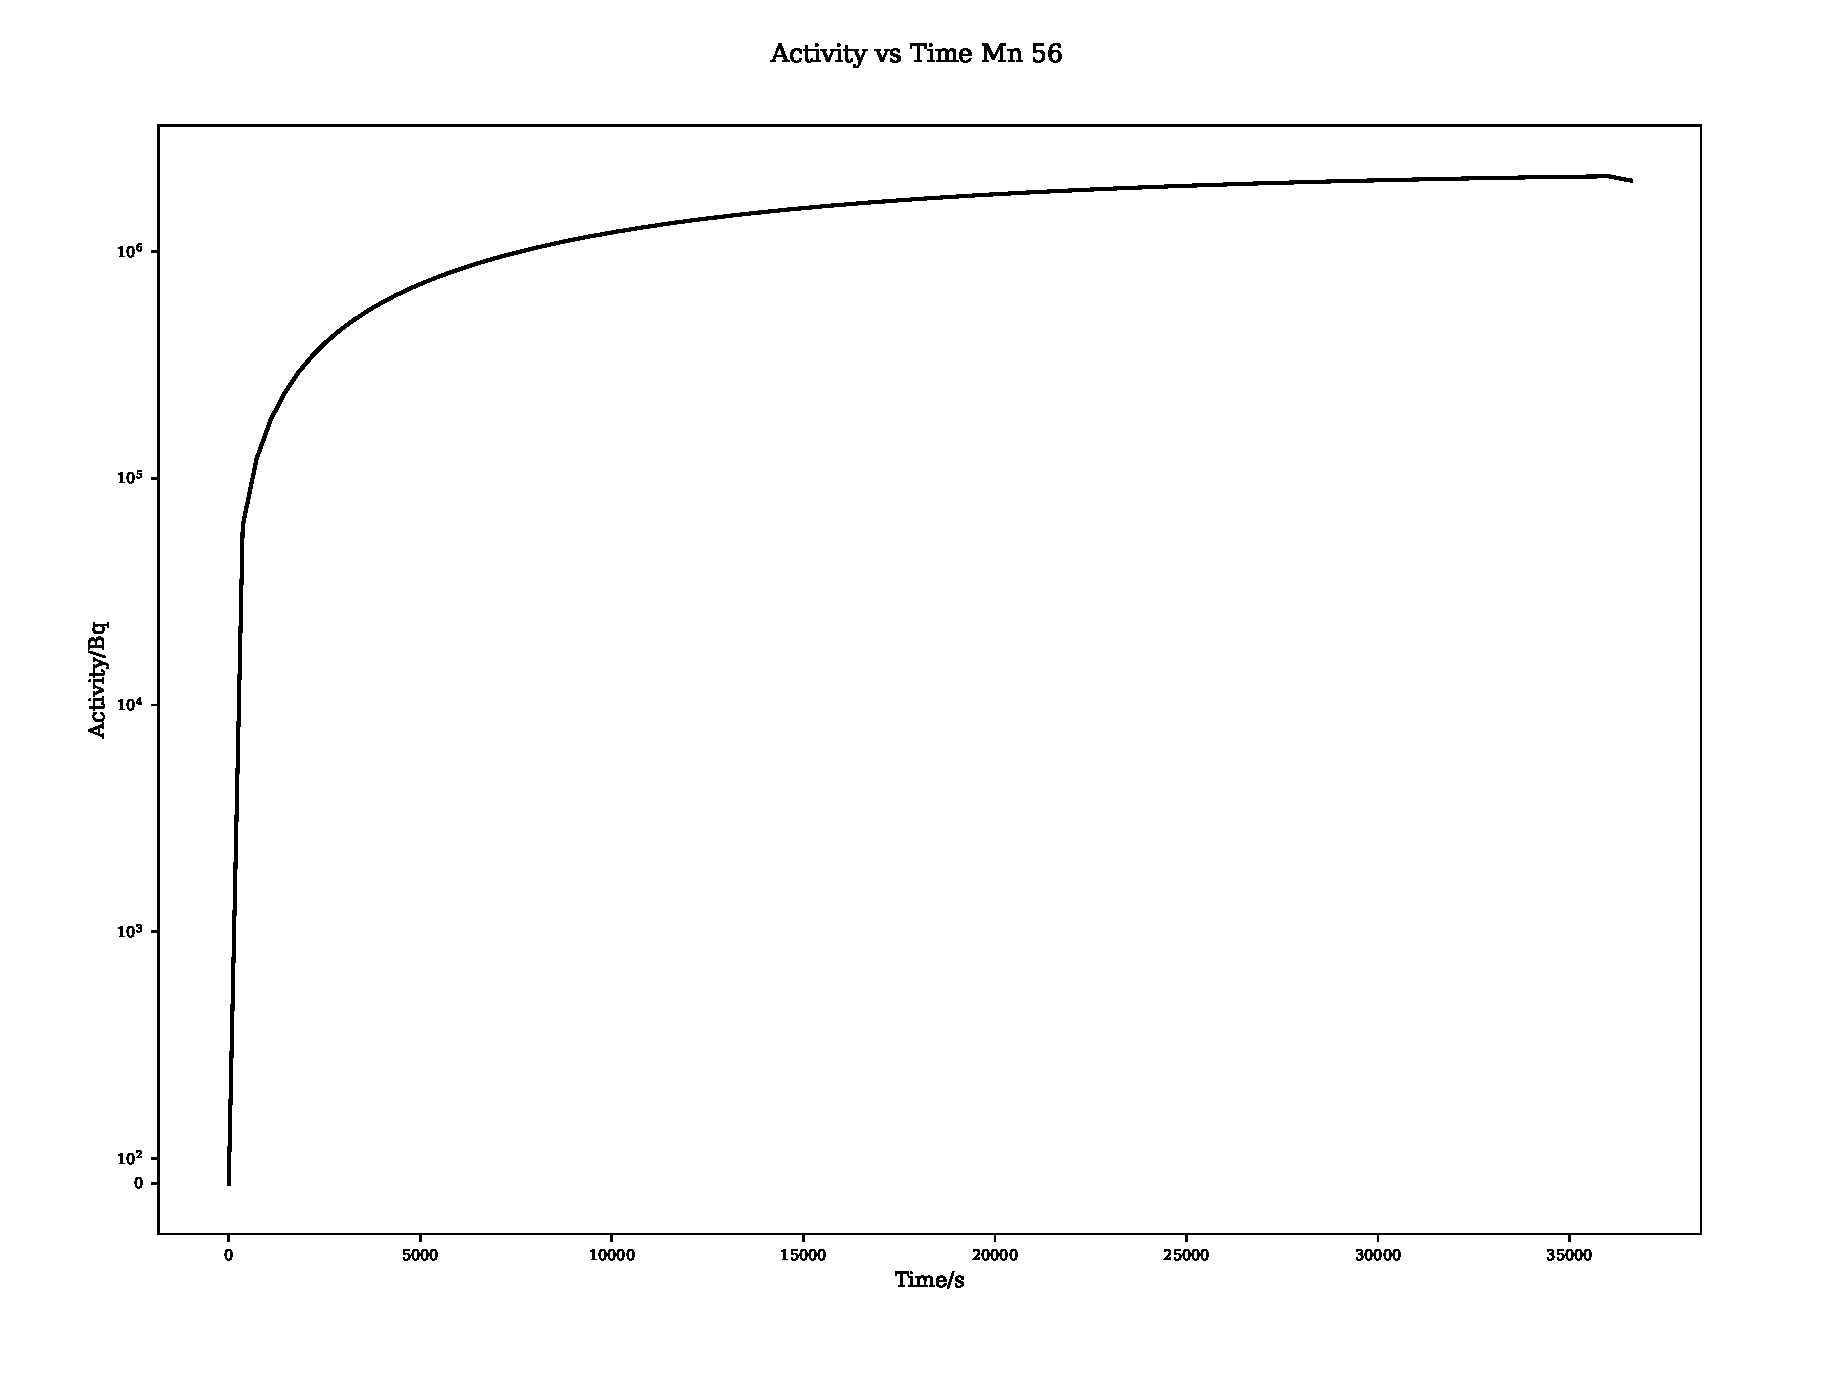
\includegraphics[width=10.0cm]{chapters/consequences_of_ionizing_radiation/neutron_plots/1/25_Mn_56_activity.eps}
    \captionsetup{font={it}}
    \caption{Predicted Mn 56 activity after neutron irradiation}
    \label{fig:mn56activity}
  \end{center}
\end{figure}

\begin{figure}
  \begin{center}
    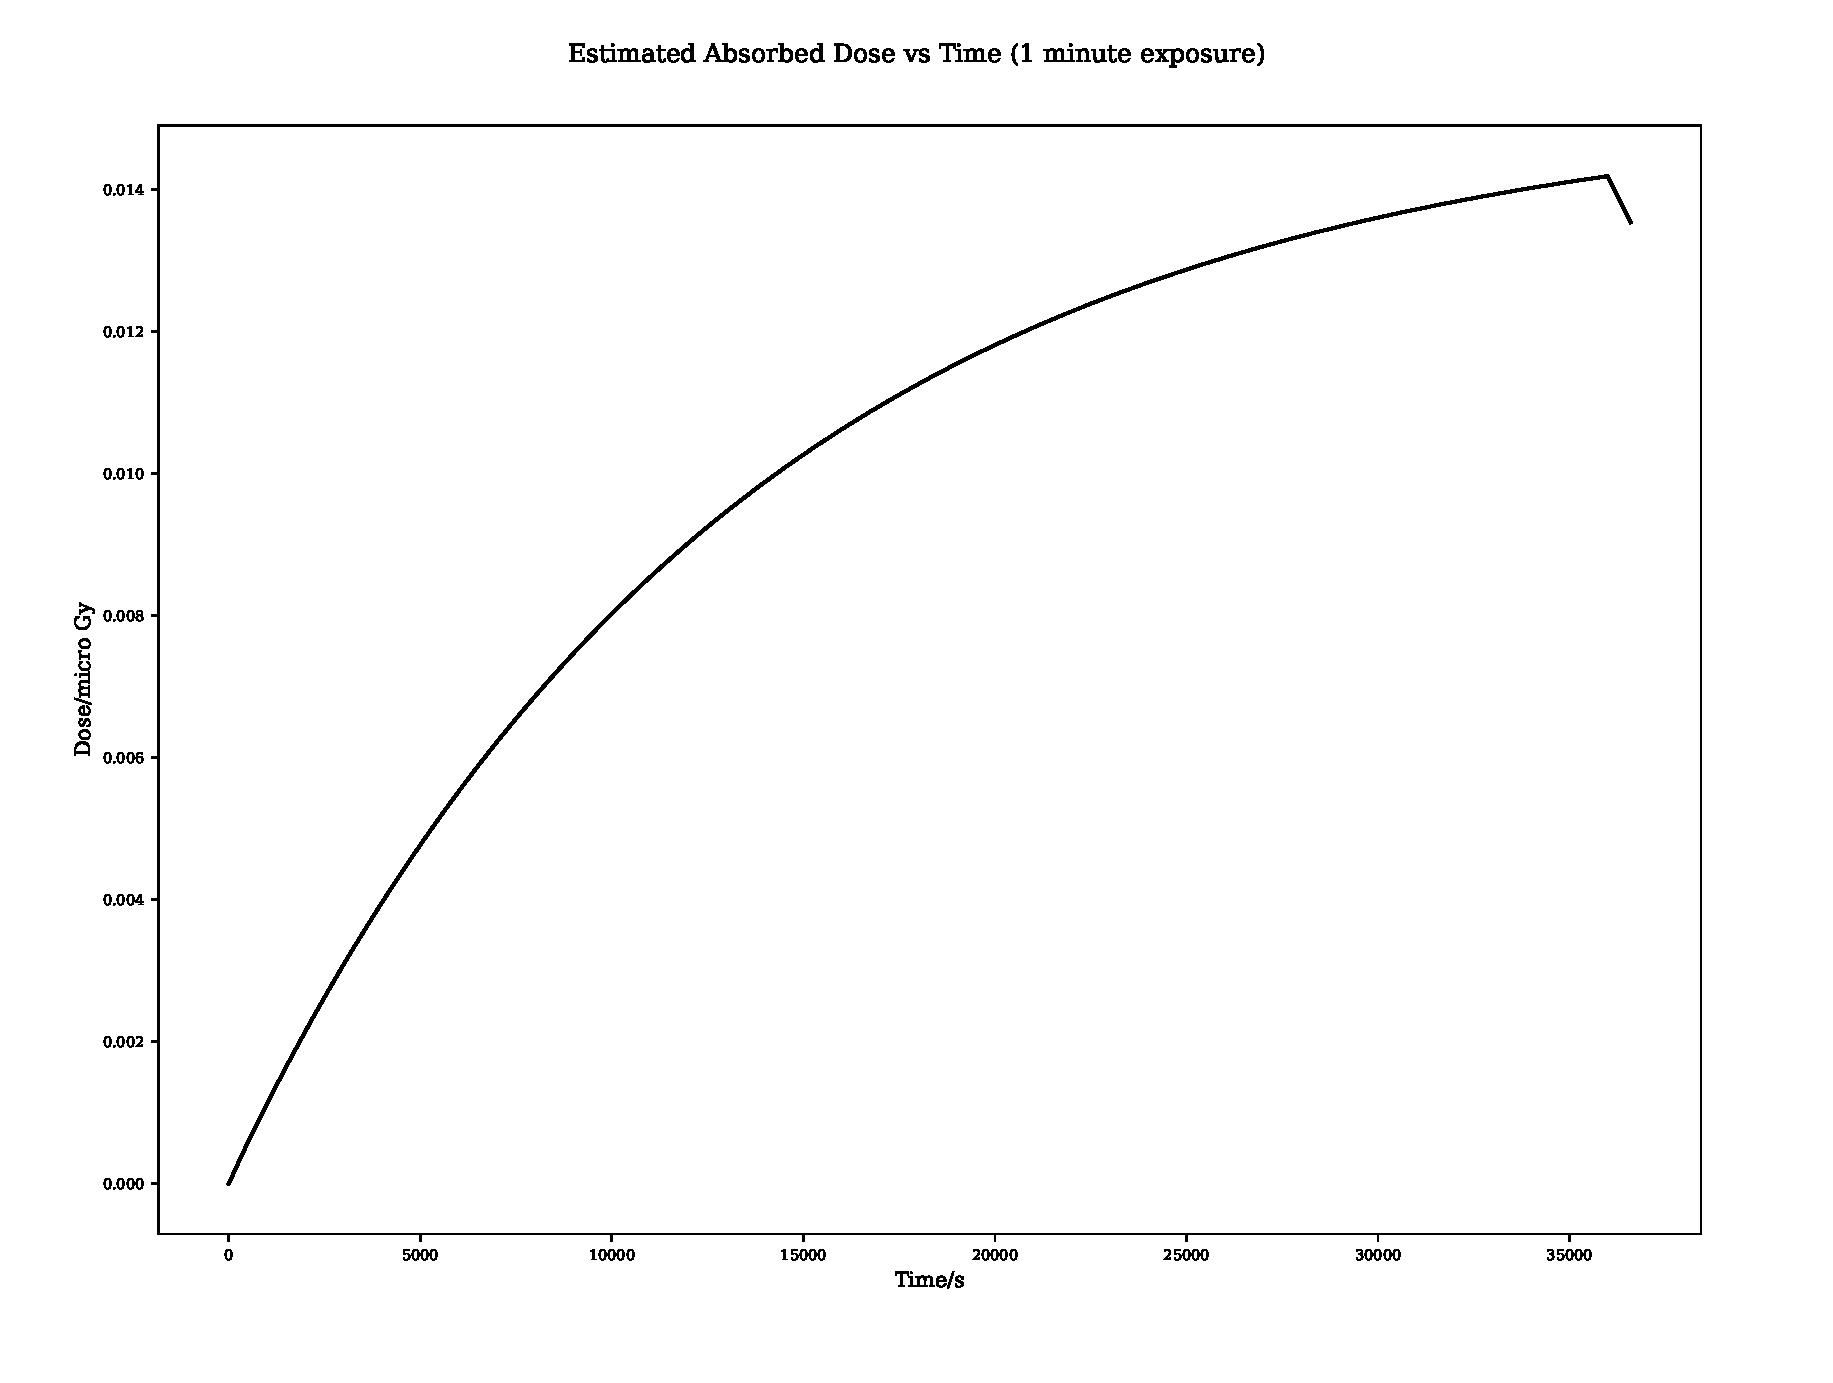
\includegraphics[width=10.0cm]{chapters/consequences_of_ionizing_radiation/neutron_plots/1/gamma_dose.eps}
    \captionsetup{font={it}}
    \caption{Steel Irradiation Gamma Dose $2.5 \times 10^7$ neutrons per cm squared per second}
    \label{fig:neutron_irradiated_steel_dose1}
  \end{center}
\end{figure}


\begin{figure}
  \begin{center}
    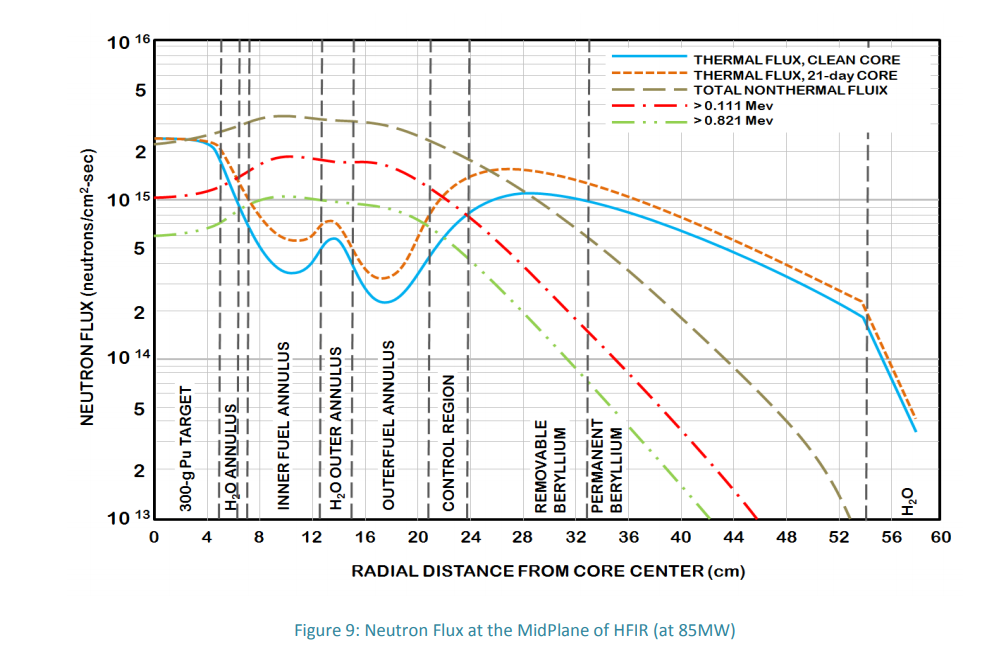
\includegraphics[width=10.0cm]{chapters/consequences_of_ionizing_radiation/images/HFIR_neutron_spectra_guide.png}
    \captionsetup{font={it}}
    \caption{High Flux Isotope Reactor Neutron Flux}
    \label{fig:hfir_neutron_flux}
  \end{center}
\end{figure}


\begin{figure}
  \begin{center}
    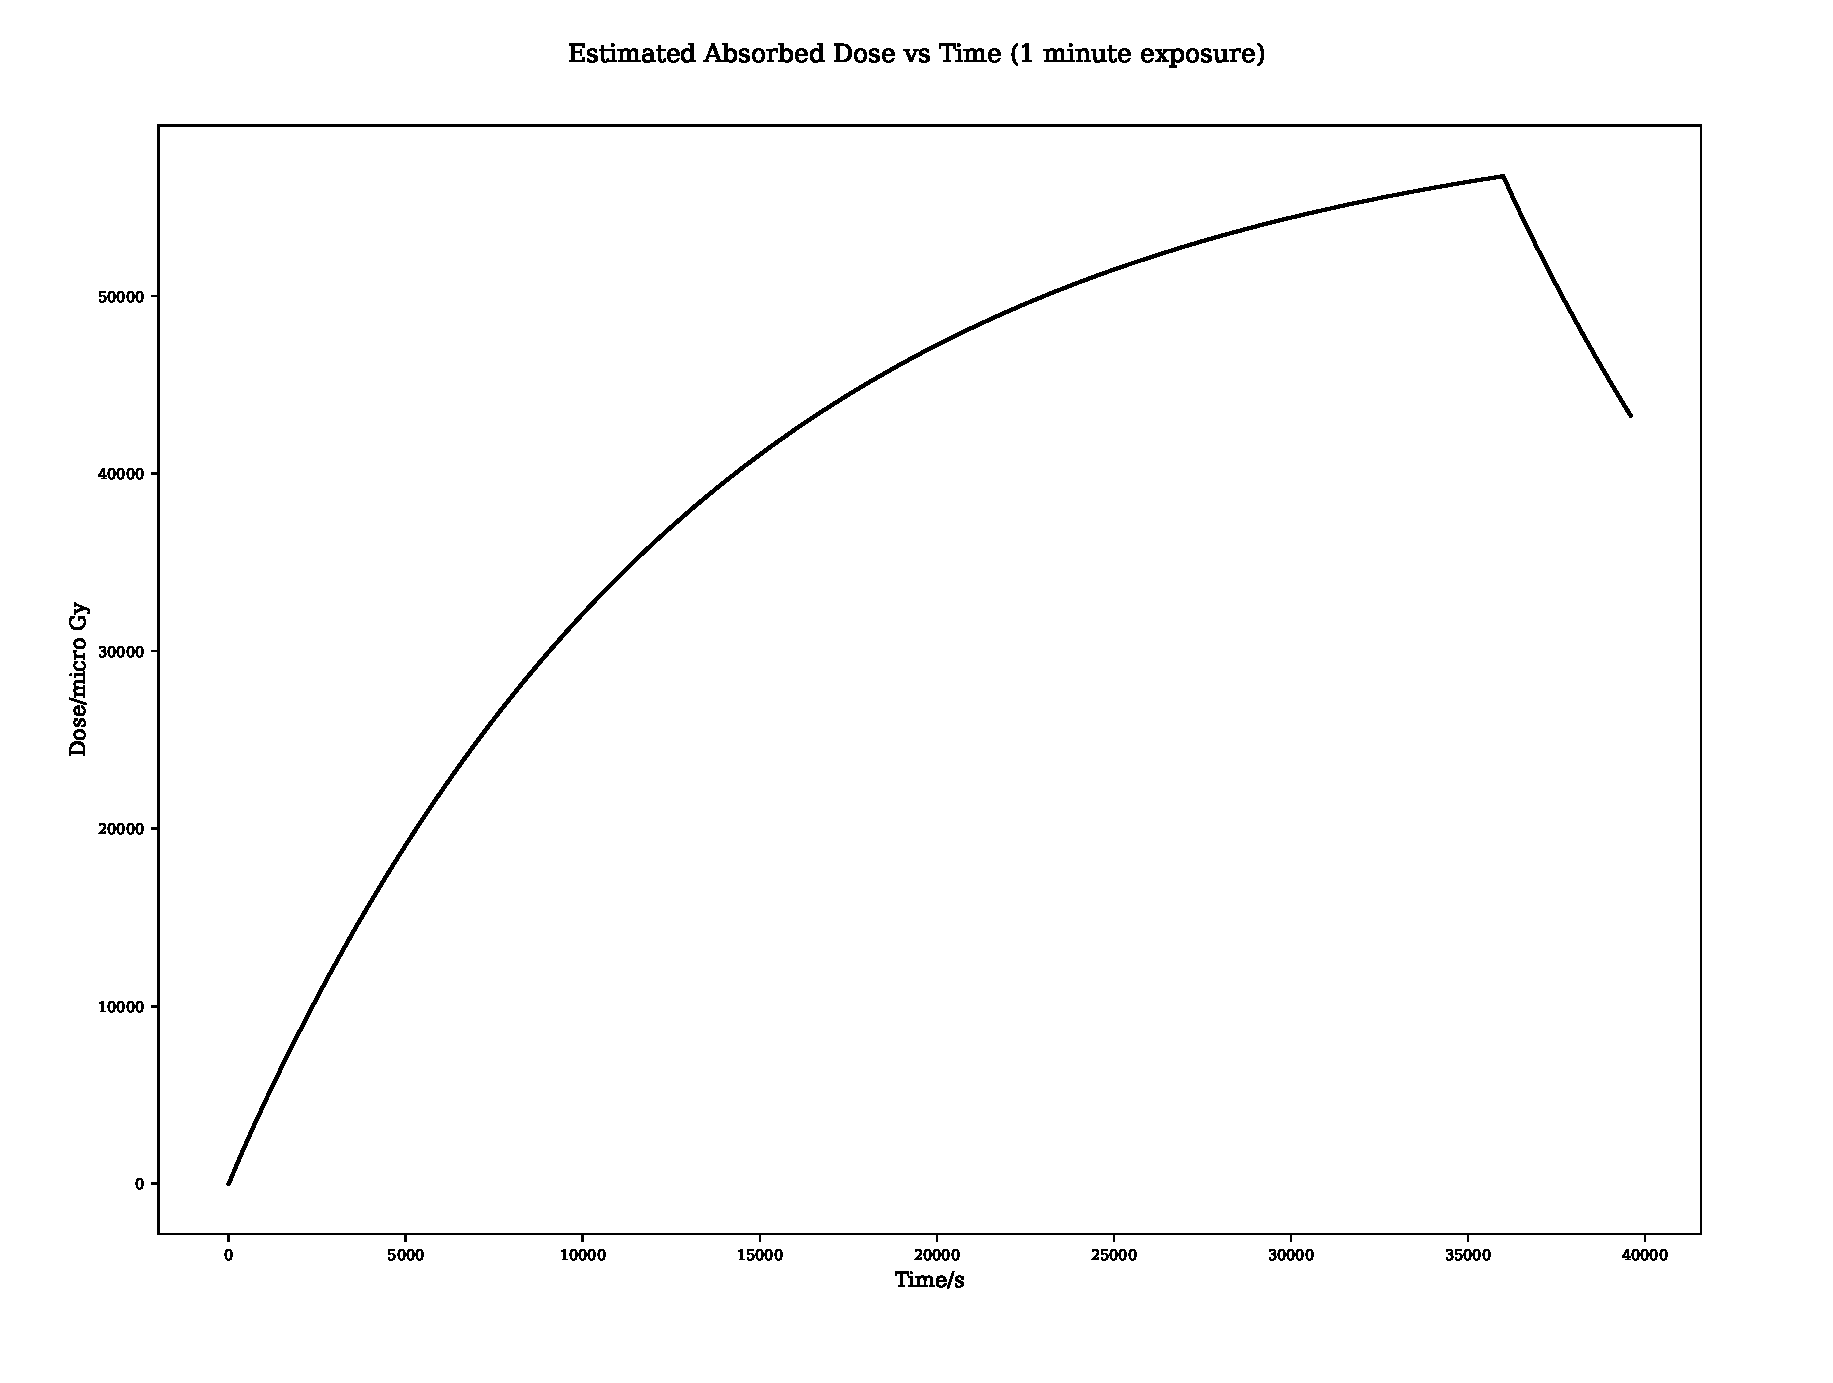
\includegraphics[width=10.0cm]{chapters/consequences_of_ionizing_radiation/neutron_plots/2/gamma_dose.eps}
    \captionsetup{font={it}}
    \caption{Steel Irradiation Gamma Dose $1.0 \times 10^{14}$ neutrons per cm squared per second}
    \label{fig:neutron_irradiated_steel_dose2}
  \end{center}
\end{figure}


\FloatBarrier

\subsubsection{Damage to Organics by Radiation}

Life evolved on Earth from single cell to multicelled organisms such as humans.  Prokaryotic cells are single celled organisms that do not have a nucleus, an example being bacteria.  Our cells are eukarytic cells, and these have a nucleus that contains the genetic information.  Millions of cells die in our body every second, and our body replaces these by replicating living cells.  During the replication stage, the DNA within the nucleus is copied.    

DNA is a polymer that is carefully constructed from six components.  Stretched out, it is approximately 2m in length and approximately 25 angstrom wide, and it is neatly contained within the cell nucleus which is on average just 6 microns across.  The structure of DNA is the well known double helix.  The sides of the helix are made from alternating sugars and phosphates, while the \enquote{rungs} of the ladder like structure are pairs of either thymine and adenine or cytosine and guanine.  These pairs are covalently bonded to the sugar-phosphate sides, and by hydrogen bonds to each other.

Mitosis is the part of the cell cycle where the DNA within the nucleus is replicated and the cell splits into two.  There are repair mechanisms, but if the DNA beyond repair, the cell may die through apoptosis, or it may replicate in an uncontrolled way leading to cancer.

Direct damage is caused when ionising radiation alters or destroys sections of DNA through a direct collision, for example a neutron colliding with and knocking out an atom in the DNA strand.

Our cells are predominantly water, so there is a higher probability of the radiation colliding with water molecules than DNA directly.  The chemistry of the contents of the cell is changed, for example by the creation of free radicals, and these lead to damage of DNA as an indirect result of radiation passing through the cell.

\begin{figure}[htb]
\centering
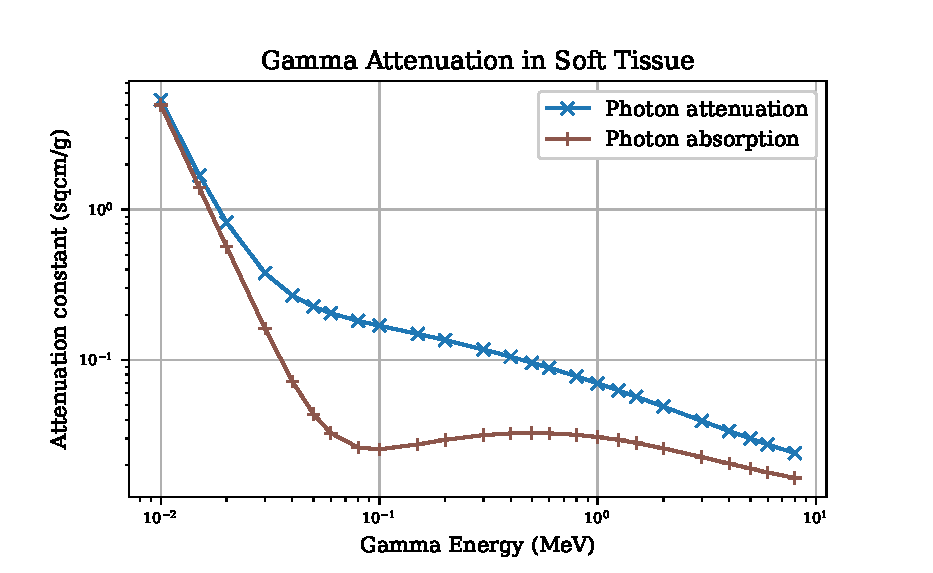
\includegraphics[width=0.5\linewidth]{chapters/consequences_of_ionizing_radiation/tissue/soft_tissue_gamma_attenuation.eps}
\caption{Dependency of absorption and attenuation of photons in soft tissue as a function of photon energy}
\label{fig:softtissueattenuation}
\end{figure}

How gamma rays interact with tissue is highly dependent upon the energy of the photons, as shown in figure \ref{fig:softtissueattenuation}.  This damage caused by radiation results in either deterministic effects or stochastic effects.  

Where there's a minor exposure to radiation, the damage caused to cells and DNA may lead to cancer later in life, or it may cause issues that are inherited from the irradiated person.  These are stochastic effects as there's a chance they could happen, but it's not certain.

Deterministic effects are due to larger doses where cells are severely damaged.  There's much less chance involved and the effects will be reproduced if multiple people are exposed.  Up to a certain dose, there is still a chance that a person would survive, but the point where the chance of death is 50\% is the \gls{ld50}, and for radiation the dose is 5Sv (table \ref{table:dosecomparison}).

The body relies heavily on three type of blood cell: erythrocytes (red cells), leukocytes (white cells) and thrombocytes (platelets).  These are produced from stem cells within bone marrow and in the course of a day billions are replaced in the body.  Large doses of radiation destroy the cells quicker than they can be produced and this leads to death.  

The lens of the eye is very sensitive to radiation and cataracts can be created by gamma rays.  Radiation can also cause damage to the gut including removal of the lining, bleeding and death.  These are examples of deterministic  effects.

Whilst it is difficult to determine the effects of radiation, particularly for stochastic effects where the effect is heavily dependent on chance, this work on calculating activity of proton irradiated targets aims to give the user a predicted activity and dose value with associated assumptions and caveats.  It is then down to the user to apply the resulting data to the situation and evaluate any health consequences.




%%%%%%%%%%%%%%%%%%%%%%%%%%%%%%%%%%%%%%%%%%%%%%%%%%%%%%%%%%%%%%%%%%%%%%%%%%%%%%%%%%%%%%%%%%%%%%%%%%%%%%%%%%
%%
%%  RADIATION DANGERS
%%
%%%%%%%%%%%%%%%%%%%%%%%%%%%%%%%%%%%%%%%%%%%%%%%%%%%%%%%%%%%%%%%%%%%%%%%%%%%%%%%%%%%%%%%%%%%%%%%%%%%%%%%%%%

\FloatBarrier

\section{Damage Cascades in Metals}

When a metal is damaged by radiation, there are microscopic defects created and removed in a very short space of time.  The result of many months or years of damage is complex and will be discussed in more detail in chapter \ref{chap:backgroundsteels}.

The cohesive energy of atoms are measured in eV (table. \ref{table:cohesiveexamples}), whereas the energy of incoming neutrons or fission fragments are measured in MeV.  Radiation in the form of electrons, protons and heavy ions will lose energy to electrons in the target as they pass through.  They may also lose energy to atoms within the lattice, knocking that atom out of place and creating a \acrshort{pka}.  Due to its neutral charge and magnetic moment, neutrons have a very weak interaction with charged particles.  They primarily lose energy directly with the nucleus of atoms within the target, also creating a \acrshort{pka}.

\begin{table}[h]
\begin{center}
\renewcommand{\arraystretch}{1.2}
\begin{tabular}{c c}
\hline\hline
Element & Cohesive Energy/eV \\
\hline\hline
Aluminium & -3.36 \\
Iron & -4.32 \\
Palladium & -3.91 \\
Platinum & -5.77 \\
Zirconium & -6.32 \\
\hline\hline
\end{tabular}
\end{center}
\caption{Cohesive Energies \cite{shengeamonline}}
\label{table:cohesiveexamples}
\end{table}

The \acrshort{pka}s create a damage cascade, and their mean recoil energy is dependent upon the energy and type of radiation.  After each cascade, there will be a period of time where the material quenches, with a recombination of some interstitials and vacancies.  The \acrshort{pka} creation and cascade thermal spike cover a time range of $10^{-18}$s to $10^{-13}$s, with the quenching phase lasting in the region of $10^{-11}$s.  However, the cumulative effect of radiation damage on a component within a reactor core may only become apparent after months or years.

\begin{table}[h]
\begin{center}
\renewcommand{\arraystretch}{1.2}
\begin{tabular}{c c}
\hline\hline
Projectile & Mean Recoil Energy \\
\hline\hline
1 MeV Electrons & 60eV \\
1 MeV protons & 200eV \\
1 MeV heavy ions & 5keV \\
1 MeV neutrons & 35keV \\
\hline\hline
\end{tabular}
\end{center}
\caption{Average recoil energy of Nickel \acrshort{pka}s\cite{gswas}}
\end{table}

The immediate aftermath of interstitials created three damage cascades is shown in fig. \ref{stollerdamage}.  Damage cascades have been the subject of a number of studies and due to their short time scale and complexity, involving thousands to millions of atoms, are studied with computer simulations.

\begin{figure}
  \begin{center}
    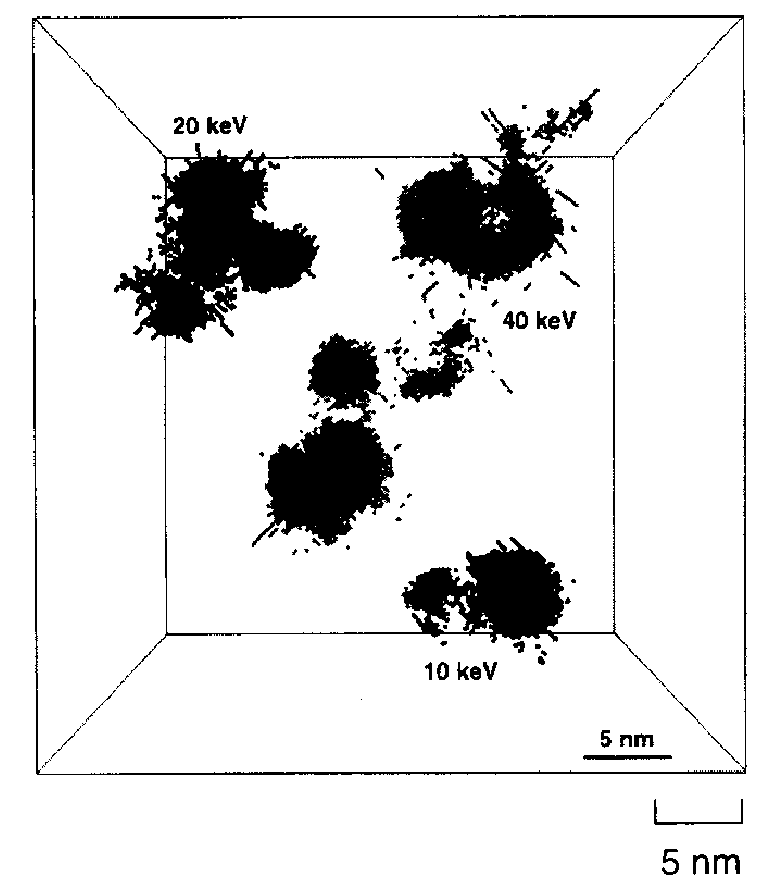
\includegraphics[width=.4\linewidth]{chapters/consequences_of_ionizing_radiation/images/stoller1996damage.png}
    \caption{Interstitials in the cascades of 10keV, 20keV and 40keV displacement cascades \cite{stollerdamage1996}}
    \label{fig:stollerdamage}
  \end{center}
\end{figure}



\newcommand{\printtikzcrystalbcc}[0]{
\fill[col_336699!10,opacity=1.0] (0.0,0.0,0.0) -- (0.0,0.0,8.0) -- (0.0,8.0,8.0) -- (0.0,8.0,0.0) -- cycle;     %% bottom square
\fill[col_336699!15,opacity=1.0] (0.0,0.0,0.0) -- (0.0,8.0,0.0) -- (8.0,8.0,0.0) -- (8.0,0.0,0.0) -- cycle;     %% bottom square
\fill[col_336699!30,opacity=1.0] (0.0,0.0,0.0) -- (8.0,0.0,0.0) -- (8.0,0.0,8.0) -- (0.0,0.0,8.0) -- cycle;     %% bottom square
\draw[solid, col_000022, very thick] (0.0,0.0,0.0) -- (0.0,4.0,0.0); 
\draw[solid, col_000022, very thick] (0.0,0.0,0.0) -- (4.0,0.0,0.0); 
\draw[solid, col_000022, very thick] (0.0,4.0,0.0) -- (0.0,8.0,0.0); 
\draw[solid, col_000022, very thick] (0.0,8.0,0.0) -- (4.0,8.0,0.0); 
\draw[solid, col_000022, very thick] (4.0,0.0,0.0) -- (8.0,0.0,0.0); 
\draw[solid, col_000022, very thick] (4.0,8.0,0.0) -- (8.0,8.0,0.0); 
\draw[solid, col_000022, very thick] (8.0,0.0,0.0) -- (8.0,4.0,0.0); 
\draw[solid, col_000022, very thick] (8.0,4.0,0.0) -- (8.0,8.0,0.0); 
\draw[dashed, col_000022, thin] (0.0,4.0,0.0) -- (4.0,4.0,0.0); 
\draw[dashed, col_000022, thin] (4.0,0.0,0.0) -- (4.0,4.0,0.0); 
\draw[dashed, col_000022, thin] (4.0,4.0,0.0) -- (4.0,8.0,0.0); 
\draw[dashed, col_000022, thin] (4.0,4.0,0.0) -- (8.0,4.0,0.0); 
\tikzdrawatom{col_333333}{0.0}{0.0}{0.0}{0.27999999999999997} 
\tikzdrawatom{col_555555}{2.0}{2.0}{0.0}{0.27999999999999997} 
\tikzdrawatom{col_666666}{0.0}{4.0}{0.0}{0.27999999999999997} 
\tikzdrawatom{col_777777}{2.0}{6.0}{0.0}{0.27999999999999997} 
\tikzdrawatom{col_333333}{0.0}{8.0}{0.0}{0.27999999999999997} 
\tikzdrawatom{col_555555}{4.0}{0.0}{0.0}{0.27999999999999997} 
\tikzdrawatom{col_666666}{6.0}{2.0}{0.0}{0.27999999999999997} 
\tikzdrawatom{col_777777}{4.0}{4.0}{0.0}{0.27999999999999997} 
\tikzdrawatom{col_333333}{6.0}{6.0}{0.0}{0.27999999999999997} 
\tikzdrawatom{col_555555}{4.0}{8.0}{0.0}{0.27999999999999997} 
\tikzdrawatom{col_666666}{8.0}{0.0}{0.0}{0.27999999999999997} 
\tikzdrawatom{col_777777}{8.0}{4.0}{0.0}{0.27999999999999997} 
\tikzdrawatom{col_666666}{8.0}{8.0}{0.0}{0.27999999999999997} 
\tikzdrawatom{col_666666}{2.0}{0.0}{2.0}{0.296063953763358} 
\tikzdrawatom{col_777777}{0.0}{2.0}{2.0}{0.296063953763358} 
\tikzdrawatom{col_333333}{2.0}{4.0}{2.0}{0.296063953763358} 
\tikzdrawatom{col_555555}{0.0}{6.0}{2.0}{0.296063953763358} 
\tikzdrawatom{col_777777}{2.0}{8.0}{2.0}{0.296063953763358} 
\tikzdrawatom{col_777777}{6.0}{0.0}{2.0}{0.296063953763358} 
\tikzdrawatom{col_333333}{4.0}{2.0}{2.0}{0.296063953763358} 
\tikzdrawatom{col_555555}{6.0}{4.0}{2.0}{0.296063953763358} 
\tikzdrawatom{col_666666}{4.0}{6.0}{2.0}{0.296063953763358} 
\tikzdrawatom{col_333333}{6.0}{8.0}{2.0}{0.296063953763358} 
\tikzdrawatom{col_555555}{8.0}{2.0}{2.0}{0.296063953763358} 
\tikzdrawatom{col_666666}{8.0}{6.0}{2.0}{0.296063953763358} 
\draw[solid, col_000022, very thick] (0.0,0.0,4.0) -- (0.0,0.0,0.0); 
\draw[solid, col_000022, very thick] (0.0,8.0,4.0) -- (0.0,8.0,0.0); 
\draw[solid, col_000022, very thick] (8.0,0.0,4.0) -- (8.0,0.0,0.0); 
\draw[solid, col_000022, very thick] (8.0,8.0,4.0) -- (8.0,8.0,0.0); 
\draw[dashed, col_000022, thin] (0.0,0.0,4.0) -- (0.0,4.0,4.0); 
\draw[dashed, col_000022, thin] (0.0,0.0,4.0) -- (4.0,0.0,4.0); 
\draw[dashed, col_000022, thin] (0.0,4.0,4.0) -- (0.0,4.0,0.0); 
\draw[dashed, col_000022, thin] (0.0,4.0,4.0) -- (0.0,8.0,4.0); 
\draw[dashed, col_000022, thin] (0.0,4.0,4.0) -- (4.0,4.0,4.0); 
\draw[dashed, col_000022, thin] (0.0,8.0,4.0) -- (4.0,8.0,4.0); 
\draw[dashed, col_000022, thin] (4.0,0.0,4.0) -- (4.0,0.0,0.0); 
\draw[dashed, col_000022, thin] (4.0,0.0,4.0) -- (4.0,4.0,4.0); 
\draw[dashed, col_000022, thin] (4.0,0.0,4.0) -- (8.0,0.0,4.0); 
\draw[dashed, col_000022, thin] (4.0,4.0,4.0) -- (4.0,4.0,0.0); 
\draw[dashed, col_000022, thin] (4.0,4.0,4.0) -- (4.0,8.0,4.0); 
\draw[dashed, col_000022, thin] (4.0,4.0,4.0) -- (8.0,4.0,4.0); 
\draw[dashed, col_000022, thin] (4.0,8.0,4.0) -- (4.0,8.0,0.0); 
\draw[dashed, col_000022, thin] (4.0,8.0,4.0) -- (8.0,8.0,4.0); 
\draw[dashed, col_000022, thin] (8.0,0.0,4.0) -- (8.0,4.0,4.0); 
\draw[dashed, col_000022, thin] (8.0,4.0,4.0) -- (8.0,4.0,0.0); 
\draw[dashed, col_000022, thin] (8.0,4.0,4.0) -- (8.0,8.0,4.0); 
\tikzdrawatom{col_333333}{0.0}{0.0}{4.0}{0.3130495168499705} 
\tikzdrawatom{col_555555}{2.0}{2.0}{4.0}{0.3130495168499705} 
\tikzdrawatom{col_666666}{0.0}{4.0}{4.0}{0.3130495168499705} 
\tikzdrawatom{col_777777}{2.0}{6.0}{4.0}{0.3130495168499705} 
\tikzdrawatom{col_666666}{0.0}{8.0}{4.0}{0.3130495168499705} 
\tikzdrawatom{col_555555}{4.0}{0.0}{4.0}{0.3130495168499705} 
\tikzdrawatom{col_666666}{6.0}{2.0}{4.0}{0.3130495168499705} 
\tikzdrawatom{col_777777}{4.0}{4.0}{4.0}{0.3130495168499705} 
\tikzdrawatom{col_333333}{6.0}{6.0}{4.0}{0.3130495168499705} 
\tikzdrawatom{col_777777}{4.0}{8.0}{4.0}{0.3130495168499705} 
\tikzdrawatom{col_333333}{8.0}{0.0}{4.0}{0.3130495168499705} 
\tikzdrawatom{col_555555}{8.0}{4.0}{4.0}{0.3130495168499705} 
\tikzdrawatom{col_555555}{8.0}{8.0}{4.0}{0.3130495168499705} 
\tikzdrawatom{col_666666}{2.0}{0.0}{6.0}{0.3310095631511115} 
\tikzdrawatom{col_777777}{0.0}{2.0}{6.0}{0.3310095631511115} 
\tikzdrawatom{col_333333}{2.0}{4.0}{6.0}{0.3310095631511115} 
\tikzdrawatom{col_555555}{0.0}{6.0}{6.0}{0.3310095631511115} 
\tikzdrawatom{col_555555}{2.0}{8.0}{6.0}{0.3310095631511115} 
\tikzdrawatom{col_777777}{6.0}{0.0}{6.0}{0.3310095631511115} 
\tikzdrawatom{col_333333}{4.0}{2.0}{6.0}{0.3310095631511115} 
\tikzdrawatom{col_555555}{6.0}{4.0}{6.0}{0.3310095631511115} 
\tikzdrawatom{col_666666}{4.0}{6.0}{6.0}{0.3310095631511115} 
\tikzdrawatom{col_666666}{6.0}{8.0}{6.0}{0.3310095631511115} 
\tikzdrawatom{col_777777}{8.0}{2.0}{6.0}{0.3310095631511115} 
\tikzdrawatom{col_333333}{8.0}{6.0}{6.0}{0.3310095631511115} 
\draw[solid, col_000022, very thick] (0.0,0.0,8.0) -- (0.0,0.0,4.0); 
\draw[solid, col_000022, very thick] (0.0,0.0,8.0) -- (0.0,4.0,8.0); 
\draw[solid, col_000022, very thick] (0.0,0.0,8.0) -- (4.0,0.0,8.0); 
\draw[solid, col_000022, very thick] (0.0,4.0,8.0) -- (0.0,8.0,8.0); 
\draw[solid, col_000022, very thick] (0.0,8.0,8.0) -- (0.0,8.0,4.0); 
\draw[solid, col_000022, very thick] (0.0,8.0,8.0) -- (4.0,8.0,8.0); 
\draw[solid, col_000022, very thick] (4.0,0.0,8.0) -- (8.0,0.0,8.0); 
\draw[solid, col_000022, very thick] (4.0,8.0,8.0) -- (8.0,8.0,8.0); 
\draw[solid, col_000022, very thick] (8.0,0.0,8.0) -- (8.0,0.0,4.0); 
\draw[solid, col_000022, very thick] (8.0,0.0,8.0) -- (8.0,4.0,8.0); 
\draw[solid, col_000022, very thick] (8.0,4.0,8.0) -- (8.0,8.0,8.0); 
\draw[solid, col_000022, very thick] (8.0,8.0,8.0) -- (8.0,8.0,4.0); 
\draw[dashed, col_000022, thin] (0.0,4.0,8.0) -- (0.0,4.0,4.0); 
\draw[dashed, col_000022, thin] (0.0,4.0,8.0) -- (4.0,4.0,8.0); 
\draw[dashed, col_000022, thin] (4.0,0.0,8.0) -- (4.0,0.0,4.0); 
\draw[dashed, col_000022, thin] (4.0,0.0,8.0) -- (4.0,4.0,8.0); 
\draw[dashed, col_000022, thin] (4.0,4.0,8.0) -- (4.0,4.0,4.0); 
\draw[dashed, col_000022, thin] (4.0,4.0,8.0) -- (4.0,8.0,8.0); 
\draw[dashed, col_000022, thin] (4.0,4.0,8.0) -- (8.0,4.0,8.0); 
\draw[dashed, col_000022, thin] (4.0,8.0,8.0) -- (4.0,8.0,4.0); 
\draw[dashed, col_000022, thin] (8.0,4.0,8.0) -- (8.0,4.0,4.0); 
\tikzdrawatom{col_333333}{0.0}{0.0}{8.0}{0.35} 
\tikzdrawatom{col_555555}{2.0}{2.0}{8.0}{0.35} 
\tikzdrawatom{col_666666}{0.0}{4.0}{8.0}{0.35} 
\tikzdrawatom{col_777777}{2.0}{6.0}{8.0}{0.35} 
\tikzdrawatom{col_333333}{0.0}{8.0}{8.0}{0.35} 
\tikzdrawatom{col_555555}{4.0}{0.0}{8.0}{0.35} 
\tikzdrawatom{col_666666}{6.0}{2.0}{8.0}{0.35} 
\tikzdrawatom{col_777777}{4.0}{4.0}{8.0}{0.35} 
\tikzdrawatom{col_333333}{6.0}{6.0}{8.0}{0.35} 
\tikzdrawatom{col_555555}{4.0}{8.0}{8.0}{0.35} 
\tikzdrawatom{col_666666}{8.0}{0.0}{8.0}{0.35} 
\tikzdrawatom{col_777777}{8.0}{4.0}{8.0}{0.35} 
\tikzdrawatom{col_333333}{8.0}{8.0}{8.0}{0.35} 
}
\newcommand{\printtikzcrystalfcc}[0]{
\fill[col_336699!10,opacity=1.0] (0.0,0.0,0.0) -- (0.0,0.0,8.0) -- (0.0,8.0,8.0) -- (0.0,8.0,0.0) -- cycle;     %% bottom square
\fill[col_336699!15,opacity=1.0] (0.0,0.0,0.0) -- (0.0,8.0,0.0) -- (8.0,8.0,0.0) -- (8.0,0.0,0.0) -- cycle;     %% bottom square
\fill[col_336699!30,opacity=1.0] (0.0,0.0,0.0) -- (8.0,0.0,0.0) -- (8.0,0.0,8.0) -- (0.0,0.0,8.0) -- cycle;     %% bottom square
\draw[solid, col_000022, very thick] (0.0,0.0,0.0) -- (0.0,4.0,0.0); 
\draw[solid, col_000022, very thick] (0.0,0.0,0.0) -- (4.0,0.0,0.0); 
\draw[solid, col_000022, very thick] (0.0,4.0,0.0) -- (0.0,8.0,0.0); 
\draw[solid, col_000022, very thick] (0.0,8.0,0.0) -- (4.0,8.0,0.0); 
\draw[solid, col_000022, very thick] (4.0,0.0,0.0) -- (8.0,0.0,0.0); 
\draw[solid, col_000022, very thick] (4.0,8.0,0.0) -- (8.0,8.0,0.0); 
\draw[solid, col_000022, very thick] (8.0,0.0,0.0) -- (8.0,4.0,0.0); 
\draw[solid, col_000022, very thick] (8.0,4.0,0.0) -- (8.0,8.0,0.0); 
\draw[dashed, col_000022, thin] (0.0,4.0,0.0) -- (4.0,4.0,0.0); 
\draw[dashed, col_000022, thin] (4.0,0.0,0.0) -- (4.0,4.0,0.0); 
\draw[dashed, col_000022, thin] (4.0,4.0,0.0) -- (4.0,8.0,0.0); 
\draw[dashed, col_000022, thin] (4.0,4.0,0.0) -- (8.0,4.0,0.0); 
\tikzdrawatom{col_333333}{0.0}{0.0}{0.0}{0.27999999999999997} 
\tikzdrawatom{col_555555}{2.0}{2.0}{0.0}{0.27999999999999997} 
\tikzdrawatom{col_666666}{0.0}{4.0}{0.0}{0.27999999999999997} 
\tikzdrawatom{col_777777}{2.0}{6.0}{0.0}{0.27999999999999997} 
\tikzdrawatom{col_333333}{0.0}{8.0}{0.0}{0.27999999999999997} 
\tikzdrawatom{col_555555}{4.0}{0.0}{0.0}{0.27999999999999997} 
\tikzdrawatom{col_666666}{6.0}{2.0}{0.0}{0.27999999999999997} 
\tikzdrawatom{col_777777}{4.0}{4.0}{0.0}{0.27999999999999997} 
\tikzdrawatom{col_333333}{6.0}{6.0}{0.0}{0.27999999999999997} 
\tikzdrawatom{col_555555}{4.0}{8.0}{0.0}{0.27999999999999997} 
\tikzdrawatom{col_666666}{8.0}{0.0}{0.0}{0.27999999999999997} 
\tikzdrawatom{col_777777}{8.0}{4.0}{0.0}{0.27999999999999997} 
\tikzdrawatom{col_666666}{8.0}{8.0}{0.0}{0.27999999999999997} 
\tikzdrawatom{col_666666}{2.0}{0.0}{2.0}{0.296063953763358} 
\tikzdrawatom{col_777777}{0.0}{2.0}{2.0}{0.296063953763358} 
\tikzdrawatom{col_333333}{2.0}{4.0}{2.0}{0.296063953763358} 
\tikzdrawatom{col_555555}{0.0}{6.0}{2.0}{0.296063953763358} 
\tikzdrawatom{col_777777}{2.0}{8.0}{2.0}{0.296063953763358} 
\tikzdrawatom{col_777777}{6.0}{0.0}{2.0}{0.296063953763358} 
\tikzdrawatom{col_333333}{4.0}{2.0}{2.0}{0.296063953763358} 
\tikzdrawatom{col_555555}{6.0}{4.0}{2.0}{0.296063953763358} 
\tikzdrawatom{col_666666}{4.0}{6.0}{2.0}{0.296063953763358} 
\tikzdrawatom{col_333333}{6.0}{8.0}{2.0}{0.296063953763358} 
\tikzdrawatom{col_555555}{8.0}{2.0}{2.0}{0.296063953763358} 
\tikzdrawatom{col_666666}{8.0}{6.0}{2.0}{0.296063953763358} 
\draw[solid, col_000022, very thick] (0.0,0.0,4.0) -- (0.0,0.0,0.0); 
\draw[solid, col_000022, very thick] (0.0,8.0,4.0) -- (0.0,8.0,0.0); 
\draw[solid, col_000022, very thick] (8.0,0.0,4.0) -- (8.0,0.0,0.0); 
\draw[solid, col_000022, very thick] (8.0,8.0,4.0) -- (8.0,8.0,0.0); 
\draw[dashed, col_000022, thin] (0.0,0.0,4.0) -- (0.0,4.0,4.0); 
\draw[dashed, col_000022, thin] (0.0,0.0,4.0) -- (4.0,0.0,4.0); 
\draw[dashed, col_000022, thin] (0.0,4.0,4.0) -- (0.0,4.0,0.0); 
\draw[dashed, col_000022, thin] (0.0,4.0,4.0) -- (0.0,8.0,4.0); 
\draw[dashed, col_000022, thin] (0.0,4.0,4.0) -- (4.0,4.0,4.0); 
\draw[dashed, col_000022, thin] (0.0,8.0,4.0) -- (4.0,8.0,4.0); 
\draw[dashed, col_000022, thin] (4.0,0.0,4.0) -- (4.0,0.0,0.0); 
\draw[dashed, col_000022, thin] (4.0,0.0,4.0) -- (4.0,4.0,4.0); 
\draw[dashed, col_000022, thin] (4.0,0.0,4.0) -- (8.0,0.0,4.0); 
\draw[dashed, col_000022, thin] (4.0,4.0,4.0) -- (4.0,4.0,0.0); 
\draw[dashed, col_000022, thin] (4.0,4.0,4.0) -- (4.0,8.0,4.0); 
\draw[dashed, col_000022, thin] (4.0,4.0,4.0) -- (8.0,4.0,4.0); 
\draw[dashed, col_000022, thin] (4.0,8.0,4.0) -- (4.0,8.0,0.0); 
\draw[dashed, col_000022, thin] (4.0,8.0,4.0) -- (8.0,8.0,4.0); 
\draw[dashed, col_000022, thin] (8.0,0.0,4.0) -- (8.0,4.0,4.0); 
\draw[dashed, col_000022, thin] (8.0,4.0,4.0) -- (8.0,4.0,0.0); 
\draw[dashed, col_000022, thin] (8.0,4.0,4.0) -- (8.0,8.0,4.0); 
\tikzdrawatom{col_333333}{0.0}{0.0}{4.0}{0.3130495168499705} 
\tikzdrawatom{col_555555}{2.0}{2.0}{4.0}{0.3130495168499705} 
\tikzdrawatom{col_666666}{0.0}{4.0}{4.0}{0.3130495168499705} 
\tikzdrawatom{col_777777}{2.0}{6.0}{4.0}{0.3130495168499705} 
\tikzdrawatom{col_666666}{0.0}{8.0}{4.0}{0.3130495168499705} 
\tikzdrawatom{col_555555}{4.0}{0.0}{4.0}{0.3130495168499705} 
\tikzdrawatom{col_666666}{6.0}{2.0}{4.0}{0.3130495168499705} 
\tikzdrawatom{col_777777}{4.0}{4.0}{4.0}{0.3130495168499705} 
\tikzdrawatom{col_333333}{6.0}{6.0}{4.0}{0.3130495168499705} 
\tikzdrawatom{col_777777}{4.0}{8.0}{4.0}{0.3130495168499705} 
\tikzdrawatom{col_333333}{8.0}{0.0}{4.0}{0.3130495168499705} 
\tikzdrawatom{col_555555}{8.0}{4.0}{4.0}{0.3130495168499705} 
\tikzdrawatom{col_555555}{8.0}{8.0}{4.0}{0.3130495168499705} 
\tikzdrawatom{col_666666}{2.0}{0.0}{6.0}{0.3310095631511115} 
\tikzdrawatom{col_777777}{0.0}{2.0}{6.0}{0.3310095631511115} 
\tikzdrawatom{col_333333}{2.0}{4.0}{6.0}{0.3310095631511115} 
\tikzdrawatom{col_555555}{0.0}{6.0}{6.0}{0.3310095631511115} 
\tikzdrawatom{col_555555}{2.0}{8.0}{6.0}{0.3310095631511115} 
\tikzdrawatom{col_777777}{6.0}{0.0}{6.0}{0.3310095631511115} 
\tikzdrawatom{col_333333}{4.0}{2.0}{6.0}{0.3310095631511115} 
\tikzdrawatom{col_555555}{6.0}{4.0}{6.0}{0.3310095631511115} 
\tikzdrawatom{col_666666}{4.0}{6.0}{6.0}{0.3310095631511115} 
\tikzdrawatom{col_666666}{6.0}{8.0}{6.0}{0.3310095631511115} 
\tikzdrawatom{col_777777}{8.0}{2.0}{6.0}{0.3310095631511115} 
\tikzdrawatom{col_333333}{8.0}{6.0}{6.0}{0.3310095631511115} 
\draw[solid, col_000022, very thick] (0.0,0.0,8.0) -- (0.0,0.0,4.0); 
\draw[solid, col_000022, very thick] (0.0,0.0,8.0) -- (0.0,4.0,8.0); 
\draw[solid, col_000022, very thick] (0.0,0.0,8.0) -- (4.0,0.0,8.0); 
\draw[solid, col_000022, very thick] (0.0,4.0,8.0) -- (0.0,8.0,8.0); 
\draw[solid, col_000022, very thick] (0.0,8.0,8.0) -- (0.0,8.0,4.0); 
\draw[solid, col_000022, very thick] (0.0,8.0,8.0) -- (4.0,8.0,8.0); 
\draw[solid, col_000022, very thick] (4.0,0.0,8.0) -- (8.0,0.0,8.0); 
\draw[solid, col_000022, very thick] (4.0,8.0,8.0) -- (8.0,8.0,8.0); 
\draw[solid, col_000022, very thick] (8.0,0.0,8.0) -- (8.0,0.0,4.0); 
\draw[solid, col_000022, very thick] (8.0,0.0,8.0) -- (8.0,4.0,8.0); 
\draw[solid, col_000022, very thick] (8.0,4.0,8.0) -- (8.0,8.0,8.0); 
\draw[solid, col_000022, very thick] (8.0,8.0,8.0) -- (8.0,8.0,4.0); 
\draw[dashed, col_000022, thin] (0.0,4.0,8.0) -- (0.0,4.0,4.0); 
\draw[dashed, col_000022, thin] (0.0,4.0,8.0) -- (4.0,4.0,8.0); 
\draw[dashed, col_000022, thin] (4.0,0.0,8.0) -- (4.0,0.0,4.0); 
\draw[dashed, col_000022, thin] (4.0,0.0,8.0) -- (4.0,4.0,8.0); 
\draw[dashed, col_000022, thin] (4.0,4.0,8.0) -- (4.0,4.0,4.0); 
\draw[dashed, col_000022, thin] (4.0,4.0,8.0) -- (4.0,8.0,8.0); 
\draw[dashed, col_000022, thin] (4.0,4.0,8.0) -- (8.0,4.0,8.0); 
\draw[dashed, col_000022, thin] (4.0,8.0,8.0) -- (4.0,8.0,4.0); 
\draw[dashed, col_000022, thin] (8.0,4.0,8.0) -- (8.0,4.0,4.0); 
\tikzdrawatom{col_333333}{0.0}{0.0}{8.0}{0.35} 
\tikzdrawatom{col_555555}{2.0}{2.0}{8.0}{0.35} 
\tikzdrawatom{col_666666}{0.0}{4.0}{8.0}{0.35} 
\tikzdrawatom{col_777777}{2.0}{6.0}{8.0}{0.35} 
\tikzdrawatom{col_333333}{0.0}{8.0}{8.0}{0.35} 
\tikzdrawatom{col_555555}{4.0}{0.0}{8.0}{0.35} 
\tikzdrawatom{col_666666}{6.0}{2.0}{8.0}{0.35} 
\tikzdrawatom{col_777777}{4.0}{4.0}{8.0}{0.35} 
\tikzdrawatom{col_333333}{6.0}{6.0}{8.0}{0.35} 
\tikzdrawatom{col_555555}{4.0}{8.0}{8.0}{0.35} 
\tikzdrawatom{col_666666}{8.0}{0.0}{8.0}{0.35} 
\tikzdrawatom{col_777777}{8.0}{4.0}{8.0}{0.35} 
\tikzdrawatom{col_333333}{8.0}{8.0}{8.0}{0.35} 
}

\newcommand{\printtikzcrystalfct}[0]{
\fill[col_336699!10,opacity=1.0] (0.0,0.0,0.0) -- (0.0,0.0,8.0) -- (0.0,8.0,8.0) -- (0.0,8.0,0.0) -- cycle;     %% bottom square
\fill[col_336699!15,opacity=1.0] (0.0,0.0,0.0) -- (0.0,8.0,0.0) -- (10.0,8.0,0.0) -- (10.0,0.0,0.0) -- cycle;     %% bottom square
\fill[col_336699!30,opacity=1.0] (0.0,0.0,0.0) -- (10.0,0.0,0.0) -- (10.0,0.0,8.0) -- (0.0,0.0,8.0) -- cycle;     %% bottom square
\draw[solid, col_000000, very thick] (0.0,0.0,4.0) -- (0.0,0.0,0.0); 
\draw[solid, col_000000, very thick] (0.0,0.0,0.0) -- (0.0,4.0,0.0); 
\draw[solid, col_000000, very thick] (0.0,0.0,0.0) -- (5.0,0.0,0.0); 
\draw[solid, col_000000, very thick] (0.0,4.0,0.0) -- (0.0,8.0,0.0); 
\draw[solid, col_000000, very thick] (0.0,8.0,4.0) -- (0.0,8.0,0.0); 
\draw[solid, col_000000, very thick] (0.0,8.0,0.0) -- (5.0,8.0,0.0); 
\draw[solid, col_000000, very thick] (5.0,0.0,0.0) -- (10.0,0.0,0.0); 
\draw[solid, col_000000, very thick] (5.0,8.0,0.0) -- (10.0,8.0,0.0); 
\draw[solid, col_000000, very thick] (10.0,0.0,4.0) -- (10.0,0.0,0.0); 
\draw[solid, col_000000, very thick] (10.0,0.0,0.0) -- (10.0,4.0,0.0); 
\draw[solid, col_000000, very thick] (10.0,4.0,0.0) -- (10.0,8.0,0.0); 
\draw[solid, col_000000, very thick] (10.0,8.0,4.0) -- (10.0,8.0,0.0); 
\draw[dashed, col_000000, thin] (0.0,4.0,4.0) -- (0.0,4.0,0.0); 
\draw[dashed, col_000000, thin] (0.0,4.0,0.0) -- (5.0,4.0,0.0); 
\draw[dashed, col_000000, thin] (5.0,0.0,4.0) -- (5.0,0.0,0.0); 
\draw[dashed, col_000000, thin] (5.0,0.0,0.0) -- (5.0,4.0,0.0); 
\draw[dashed, col_000000, thin] (5.0,4.0,4.0) -- (5.0,4.0,0.0); 
\draw[dashed, col_000000, thin] (5.0,4.0,0.0) -- (5.0,8.0,0.0); 
\draw[dashed, col_000000, thin] (5.0,4.0,0.0) -- (10.0,4.0,0.0); 
\draw[dashed, col_000000, thin] (5.0,8.0,4.0) -- (5.0,8.0,0.0); 
\draw[dashed, col_000000, thin] (10.0,4.0,4.0) -- (10.0,4.0,0.0); 
\tikzdrawatom{col_333333}{0.0}{0.0}{0.0}{0.27999999999999997} 
\tikzdrawatom{col_555555}{0.0}{4.0}{0.0}{0.27999999999999997} 
\tikzdrawatom{col_333333}{0.0}{8.0}{0.0}{0.27999999999999997} 
\tikzdrawatom{col_555555}{5.0}{0.0}{0.0}{0.27999999999999997} 
\tikzdrawatom{col_666666}{5.0}{4.0}{0.0}{0.27999999999999997} 
\tikzdrawatom{col_555555}{5.0}{8.0}{0.0}{0.27999999999999997} 
\tikzdrawatom{col_333333}{10.0}{0.0}{0.0}{0.27999999999999997} 
\tikzdrawatom{col_777777}{10.0}{4.0}{0.0}{0.27999999999999997} 
\tikzdrawatom{col_666666}{10.0}{8.0}{0.0}{0.27999999999999997} 
\tikzdrawatom{col_777777}{2.5}{2.0}{2.0}{0.296063953763358} 
\tikzdrawatom{col_333333}{2.5}{6.0}{2.0}{0.296063953763358} 
\tikzdrawatom{col_333333}{7.5}{2.0}{2.0}{0.296063953763358} 
\tikzdrawatom{col_555555}{7.5}{6.0}{2.0}{0.296063953763358} 
\draw[solid, col_000000, very thick] (0.0,0.0,8.0) -- (0.0,0.0,4.0); 
\draw[solid, col_000000, very thick] (0.0,8.0,8.0) -- (0.0,8.0,4.0); 
\draw[solid, col_000000, very thick] (10.0,0.0,8.0) -- (10.0,0.0,4.0); 
\draw[solid, col_000000, very thick] (10.0,8.0,8.0) -- (10.0,8.0,4.0); 
\draw[dashed, col_000000, thin] (0.0,0.0,4.0) -- (0.0,4.0,4.0); 
\draw[dashed, col_000000, thin] (0.0,0.0,4.0) -- (5.0,0.0,4.0); 
\draw[dashed, col_000000, thin] (0.0,4.0,8.0) -- (0.0,4.0,4.0); 
\draw[dashed, col_000000, thin] (0.0,4.0,4.0) -- (0.0,8.0,4.0); 
\draw[dashed, col_000000, thin] (0.0,4.0,4.0) -- (5.0,4.0,4.0); 
\draw[dashed, col_000000, thin] (0.0,8.0,4.0) -- (5.0,8.0,4.0); 
\draw[dashed, col_000000, thin] (5.0,0.0,8.0) -- (5.0,0.0,4.0); 
\draw[dashed, col_000000, thin] (5.0,0.0,4.0) -- (5.0,4.0,4.0); 
\draw[dashed, col_000000, thin] (5.0,0.0,4.0) -- (10.0,0.0,4.0); 
\draw[dashed, col_000000, thin] (5.0,4.0,8.0) -- (5.0,4.0,4.0); 
\draw[dashed, col_000000, thin] (5.0,4.0,4.0) -- (5.0,8.0,4.0); 
\draw[dashed, col_000000, thin] (5.0,4.0,4.0) -- (10.0,4.0,4.0); 
\draw[dashed, col_000000, thin] (5.0,8.0,8.0) -- (5.0,8.0,4.0); 
\draw[dashed, col_000000, thin] (5.0,8.0,4.0) -- (10.0,8.0,4.0); 
\draw[dashed, col_000000, thin] (10.0,0.0,4.0) -- (10.0,4.0,4.0); 
\draw[dashed, col_000000, thin] (10.0,4.0,8.0) -- (10.0,4.0,4.0); 
\draw[dashed, col_000000, thin] (10.0,4.0,4.0) -- (10.0,8.0,4.0); 
\tikzdrawatom{col_666666}{0.0}{0.0}{4.0}{0.3130495168499705} 
\tikzdrawatom{col_777777}{0.0}{4.0}{4.0}{0.3130495168499705} 
\tikzdrawatom{col_777777}{0.0}{8.0}{4.0}{0.3130495168499705} 
\tikzdrawatom{col_777777}{5.0}{0.0}{4.0}{0.3130495168499705} 
\tikzdrawatom{col_333333}{5.0}{4.0}{4.0}{0.3130495168499705} 
\tikzdrawatom{col_333333}{5.0}{8.0}{4.0}{0.3130495168499705} 
\tikzdrawatom{col_777777}{10.0}{0.0}{4.0}{0.3130495168499705} 
\tikzdrawatom{col_666666}{10.0}{4.0}{4.0}{0.3130495168499705} 
\tikzdrawatom{col_555555}{10.0}{8.0}{4.0}{0.3130495168499705} 
\tikzdrawatom{col_555555}{2.5}{2.0}{6.0}{0.3310095631511115} 
\tikzdrawatom{col_666666}{2.5}{6.0}{6.0}{0.3310095631511115} 
\tikzdrawatom{col_666666}{7.5}{2.0}{6.0}{0.3310095631511115} 
\tikzdrawatom{col_777777}{7.5}{6.0}{6.0}{0.3310095631511115} 
\draw[solid, col_000000, very thick] (0.0,0.0,8.0) -- (0.0,4.0,8.0); 
\draw[solid, col_000000, very thick] (0.0,0.0,8.0) -- (5.0,0.0,8.0); 
\draw[solid, col_000000, very thick] (0.0,4.0,8.0) -- (0.0,8.0,8.0); 
\draw[solid, col_000000, very thick] (0.0,8.0,8.0) -- (5.0,8.0,8.0); 
\draw[solid, col_000000, very thick] (5.0,0.0,8.0) -- (10.0,0.0,8.0); 
\draw[solid, col_000000, very thick] (5.0,8.0,8.0) -- (10.0,8.0,8.0); 
\draw[solid, col_000000, very thick] (10.0,0.0,8.0) -- (10.0,4.0,8.0); 
\draw[solid, col_000000, very thick] (10.0,4.0,8.0) -- (10.0,8.0,8.0); 
\draw[dashed, col_000000, thin] (0.0,4.0,8.0) -- (5.0,4.0,8.0); 
\draw[dashed, col_000000, thin] (5.0,0.0,8.0) -- (5.0,4.0,8.0); 
\draw[dashed, col_000000, thin] (5.0,4.0,8.0) -- (5.0,8.0,8.0); 
\draw[dashed, col_000000, thin] (5.0,4.0,8.0) -- (10.0,4.0,8.0); 
\tikzdrawatom{col_333333}{0.0}{0.0}{8.0}{0.35} 
\tikzdrawatom{col_555555}{0.0}{4.0}{8.0}{0.35} 
\tikzdrawatom{col_666666}{0.0}{8.0}{8.0}{0.35} 
\tikzdrawatom{col_555555}{5.0}{0.0}{8.0}{0.35} 
\tikzdrawatom{col_666666}{5.0}{4.0}{8.0}{0.35} 
\tikzdrawatom{col_777777}{5.0}{8.0}{8.0}{0.35} 
\tikzdrawatom{col_666666}{10.0}{0.0}{8.0}{0.35} 
\tikzdrawatom{col_555555}{10.0}{4.0}{8.0}{0.35} 
\tikzdrawatom{col_333333}{10.0}{8.0}{8.0}{0.35} 
}
%%%%%%%%%%%%%%%%%%%%%%%%%%%%%%%%%%%%%%%%%%%%%%%%%%%%%%%%%%%%%%%%%%%%%%%%%%%%%%%%%%%%%%%%%%%%%%%%%%%%%%%%%%
%%
%%  Austenitic Steels
%%
%%%%%%%%%%%%%%%%%%%%%%%%%%%%%%%%%%%%%%%%%%%%%%%%%%%%%%%%%%%%%%%%%%%%%%%%%%%%%%%%%%%%%%%%%%%%%%%%%%%%%%%%%%




\chapter[Austenitic Steels in Nuclear Power]{Austenitic Steels in Nuclear Power}
\label{chap:backgroundsteels}

\begin{changemargin}{1.0cm}{1.0cm}
\abstractpreamble{Austenitic stainless steels have played an important role in the nuclear industry.  They have a good resistance to corrosion and behave well at moderately high temperatures, having a good resistance to creep.  They have been used within the primary circuit and secondary circuit of power stations, as cladding for fuel pellets, in the steam dryers, pre-heater tubing, core structurals, primary piping and more.  Ferritic steel is magnetic and has a \acrshort{bcc} structure, whereas austenitic steel is non-magnetic with a \acrshort{fcc} structure, with its high Nickel content stabilising this phase.  An area of concern is the susceptibility of austenitic stainless steels to \acrshort{igscc}.}
\end{changemargin}


%%%%%%%%%%%%%%%%%%%%%%%%%%%%%%%%%%%%%%%%%%%%%%%%%%%%%%%%%%%%%%%%%%%%%%%%%%%%%%%%%%%%%%%%%%%%%%%%%%%%%%%%%%
%%
%%  Stainless Steels
%%
%%%%%%%%%%%%%%%%%%%%%%%%%%%%%%%%%%%%%%%%%%%%%%%%%%%%%%%%%%%%%%%%%%%%%%%%%%%%%%%%%%%%%%%%%%%%%%%%%%%%%%%%%%


\section{Stainless Steel}

\subsection{Introduction}

Stainless steel is a relatively new material, having first been developed and refined from the 1800s to the early 1900s, then being defined as a steel with at least 10.5\% \Gls{Cr} in 1911.  The addition of \Gls{Cr} to this level causes the formation of a passive protective layer of chromium oxide.  

\Gls{Fe} is alloyed with \Gls{Cr}, \Gls{Ni} and \Gls{C} in varying quantities to make Stainless Steel.  Depending on the application, other elements, such as \Gls{Mo}, may be added to enhance the properties of the steel.

\subsection{Grades of Stainless Steel}

While the criteria that qualifies an alloy as Stainless Steel is containing Fe, \Gls{C} and at least 10.5\% Cr, there are many grades that have a variety of properties and atomic structures.  The composition influences the structure and other properties such as resistance to corrosion, yield strength, creep resistance and whether the steel is magnetic or not.

Both Fe and Cr are \acrshort{bcc} at standard temperatures and pressures, but adding austenite stabilisers such as Ni, Mn or C, the structure of the steel can be altered from \acrshort{bcc} to \acrshort{fcc}.  Balancing the proportion of these elements changes the phase of the steel, and this may be represented as a Schaeffler diagram (fig. \ref{fig:FeCrNiSchaeffler}\cite{fecrschaeffler}) or a ternary phase diagram (fig. \ref{fig:FeCrNi-PhaseDiagram}\cite{fenicrternaryphase}).

\begin{figure}
\centering
\begin{minipage}{.46\textwidth}
\centering
    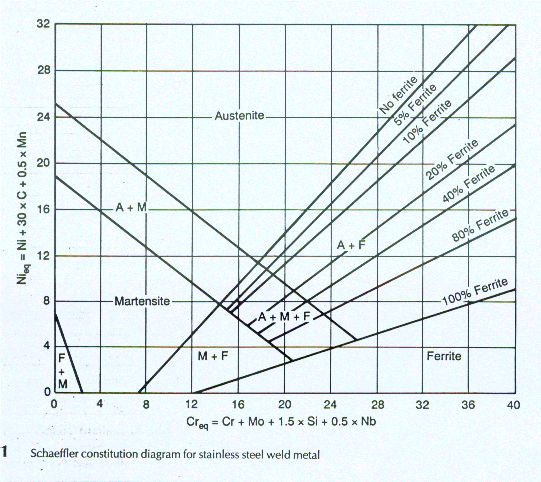
\includegraphics[width=.9\linewidth]{chapters/austenitic_steels_in_nuclear/plots/fecrschaeffler.png}
    \caption{Steel Cr-Ni Schaeffler Diagram\cite{fecrschaeffler}}
    \label{fig:FeCrNiSchaeffler}
\end{minipage}
\begin{minipage}{.46\textwidth}
\centering
  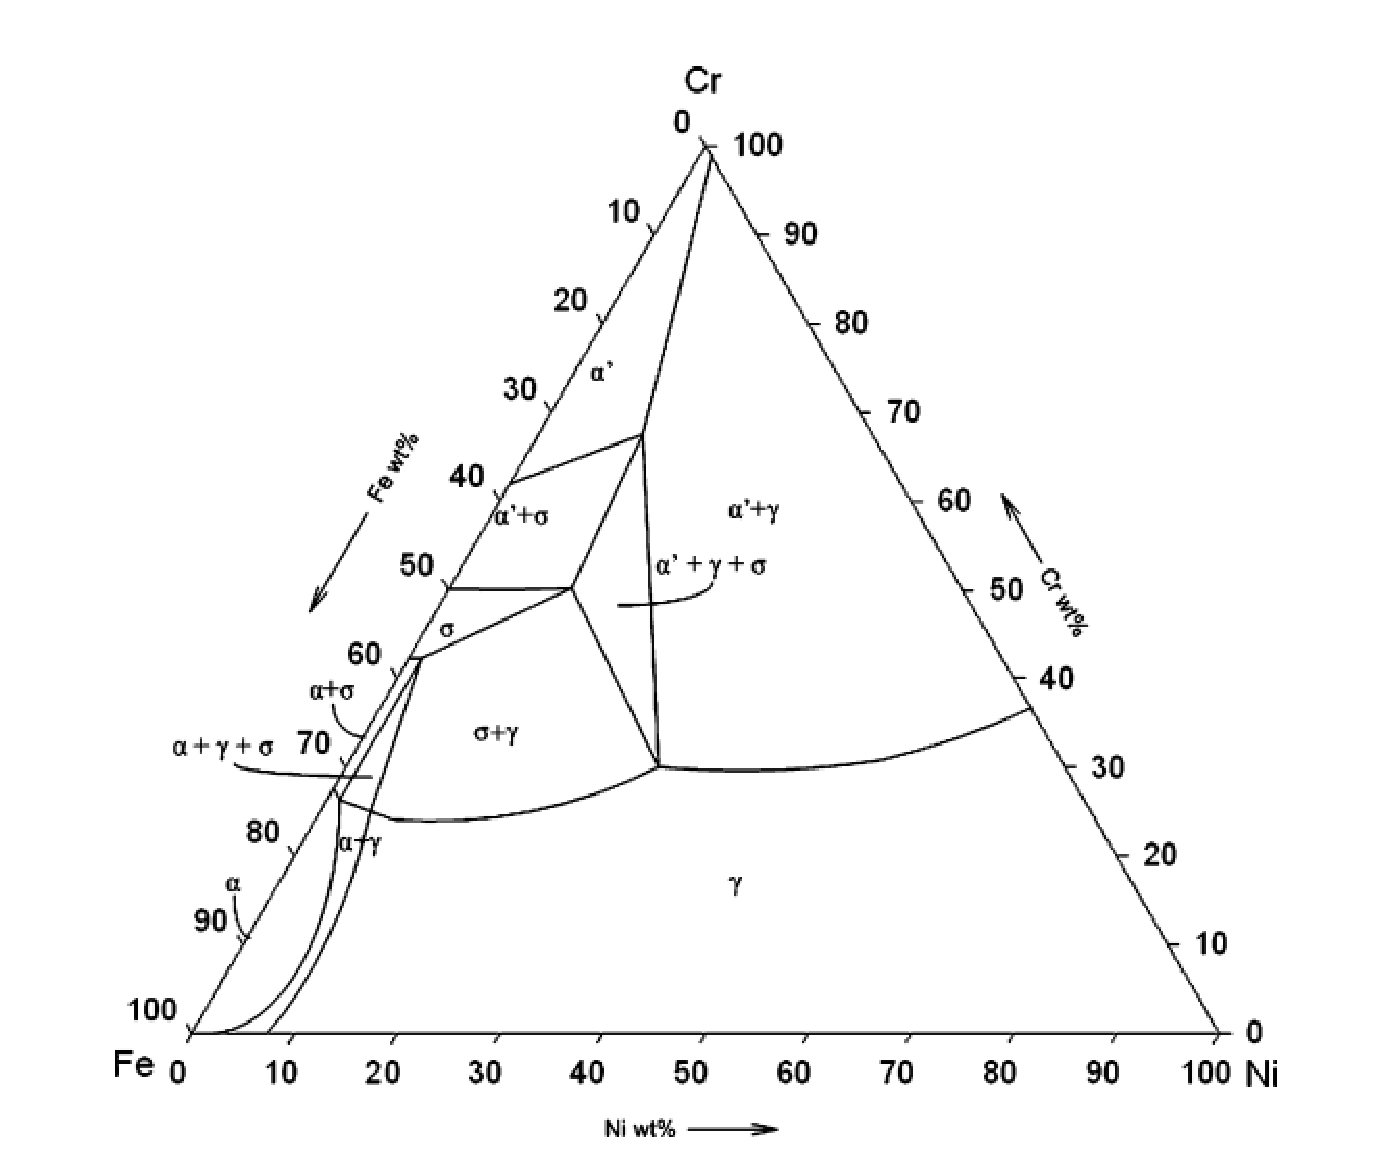
\includegraphics[width=.9\linewidth]{chapters/austenitic_steels_in_nuclear/plots/FeCrNi}
  \caption{Iron-Chromium-Nickel Phase Diagram\cite{fenicrternaryphase}}
  \label{fig:FeCrNi-PhaseDiagram}
\end{minipage}
\begin{minipage}{.05\textwidth}
\end{minipage}
\end{figure}


\subsubsection{Ferritic Stainless Steel}


\begin{figure}[ht]
\centering
\begin{tikzpicture}[scale=0.40]
\printtikzcrystalbcc{}
\end{tikzpicture} 
\caption{\acrshort{bcc} structure of ferritic stainless steel - a 2x2x2 supercell\cite{tikzcrystal}}
\label{fig:steelbcc}
\end{figure} 

At room temperatures and pressures, Fe exists in the alpha phase, which is a \acrshort{bcc} crystal.  It is energetically favourable for the magnetic moments of the Fe atoms to align with one another ferromagnetically.  Ferritic stainless steels also have the natural alpha phase crystal structure of pure Fe at room temperature which is \acrshort{bcc} (fig \ref{fig:steelbcc}).  These steels are magnetic and may be hardened by cold working.  They are less corrosion resistant than austenitic stainless steels.  Two common examples of this grade of steel are \acrlong{asme} codes 405 and 430.



\subsubsection{Austenitic Stainless Steel}

\begin{figure}[ht]
\centering
\begin{tikzpicture}[scale=0.40]
\printtikzcrystalfcc{}
\end{tikzpicture} 
\caption{\acrshort{fcc} structure of austenitic stainless steel - a 2x2x2 supercell\cite{tikzcrystal}}
\label{fig:steelfcc}
\end{figure} 

Austenite is a \acrshort{fcc} \gls{allotrope} of Fe (fig \ref{fig:steelfcc}), and austenitic stainless steels are useful in many applications, including a structural material for nuclear plant components, due to their resistance to corrosion.  In addition to 10.5 wt\% or more Cr they require an austenite stabilising element to be added.  

Two examples of such steels are \acrshort{asme} codes 304 and 316.  Both have a high Cr content, in the region of 18-20\%, which is in excess of the minimum passive film requirement of around 10-11\%.  The natural structure of such an Fe-Cr alloy would be \acrshort{bcc}, however 304 and 316 Steels contain Ni (approximately 8\% and 10\% respectively) which stabilises the austenite phase and is responsible for the \acrshort{fcc} structure of the steel.  The 316 grade contains a minimum of 2\% Mo to improve its resistance to corrosion.

Ferritic and martensitic have a better resistance to thermal or swelling shock than austenitic \cite{bccfenimodel}, but the corrosion resistance of austenitic steels is a deciding factor when choosing a steel for an application where corrosion resistance is important.



\subsubsection{Martensitic Stainless Steel}

Martensitic stainless steels have a \acrshort{fcc} structure at high temperature, but when heat treated take on a \acrshort{bcc}  structure.  This allows martensitic, unlike austenitic and ferritic, to be hardened by heat treatment.  These steels are magnetic, they contain more than 10.5\% Cr but have a much lower Ni than austenitic grades, if any.  They are corrosion resistant, but the corrosion resistance of austenitic steel is typically better.  Two examples of such steels are ASME codes 410 and 431. 




%%%%%%%%%%%%%%%%%%%%%%%%%%%%%%%%%%%%%%%%%%%%%%%%%%%%%%%%%%%%%%%%%%%%%%%%%%%%%%%%%%%%%%%%%%%%%%%%%%%%%%%%%%
%%
%%  Austenitic Steels
%%
%%%%%%%%%%%%%%%%%%%%%%%%%%%%%%%%%%%%%%%%%%%%%%%%%%%%%%%%%%%%%%%%%%%%%%%%%%%%%%%%%%%%%%%%%%%%%%%%%%%%%%%%%%



\section[Use In Reactors]{Austenitic Steels in Nuclear Reactors}

\subsection{The Use of Austenintic Steels in Reactors}

Austenitic stainless steels are known to have better corrosion resistance when compared to their ferritic and martensitic counterparts.  Due to this and their excellent strength, austenitic steels have been widely used in nuclear reactors.  The cheaper to manufacture \gls{304SS} and more corrosion resistant \gls{316SS} have been particularly popular choices of steel.  There are drawbacks when compared to ferritic and martensitic steels, and two in particular are \acrshort{igscc} and swelling.



\subsection{Atom Damage Cascades}

Fission fragments carry away the majority of the energy released during fission, with an approximate energy of 170MeV per 235U fission event.  The fragments are large and have a highly charged positive nucleus that stops rapidly due to the Coulomb interaction with the nuclei of surrounding atoms.  Electrons released by beta decay travel a greater distance; they lose energy by interacting with electrons, but may also knock atoms out of place.  Neutrons travel further still and lose energy by interacting directly with the nuclei of the surrounding material.

When an incoming projectile hits an atom in the target material, this atom becomes the \acrfull{pka}.  This \acrshort{pka} is knocked out of its place and loses energy by colliding with other atoms and through electronic stopping.  If its energy is high enough it will cause a damage cascade through the material.  Atoms knocked out of their regular position in the crystal lattice leave vacancies behind.  The displaced atoms either recombine with vacancies, become interstitial atoms or diffuse to defect sinks.  

The damage event has four main phases over a short period of time\cite{gswasdamage}:

\begin{itemize}
\item \acrshort{pka} creation ($~ 10^{-18}s$)
\item cascade and thermal spike ($~ 10^{-13}s$)
\item quench ($~ 10^{-11}s$)
\item annealing and defect migration ($~ 10^{-9}s$)
\end{itemize}

These individual damage events happen over a very small amount of time, but a number of complex problems arise as a result of this damage over a much longer time period.  The damage to components can take many years and high damage doses to manifest on a macroscopic scale.


\subsection{Damage Rates}
\FloatBarrier

The safety of a Nuclear reactor is the primary concern; it must generate power, but it must be safe.  It must also be cost efficient.  \acrshort{gen2} \acrshort{pwr} fuel assembles were expected to withstand several \acrshort{dpa}\cite{genIVstrucmat}.  In \acrshort{bwr}s the materials are designed to be irradiated by a total fluence of $10^{22} n cm^{-2}$, experiencing approximately 7 \acrshort{dpa} over the lifetime of the components\cite{lightwaterallenbusby}.  Components in \acrshort{pwr}s are irradiated by up to a total fluence of $10^{23} n cm^{-2}$, and are expected to operate up to an irradiation dose of 70 \acrshort{dpa}\cite{lightwaterallenbusby}.  To remain cost efficient, components in \acrshort{gen4} reactors will be expected to operate safely up to even higher doses or irradiation damage (fig \ref{fig:genIVdpa}).  Components in sodium-cooled fast reactors will be expected to withstand up to 200 \acrshort{dpa} over their lifetime to meet the requirements of cost effectiveness and durability\cite{genIVstrucmat}.


\begin{figure}[h]
  \begin{center}
    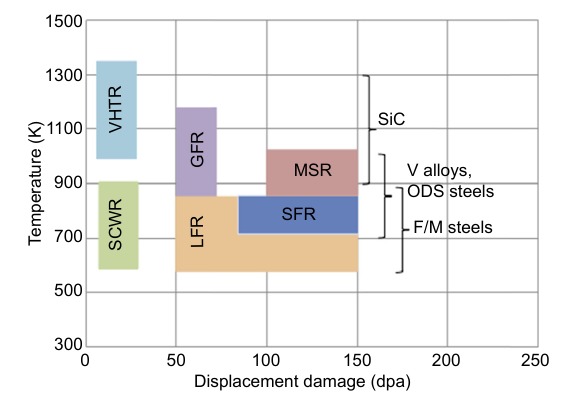
\includegraphics[scale=0.60]{chapters/austenitic_steels_in_nuclear/images/dpagenIV.png}
    \caption{Expected \acrshort{dpa} during component life time and operating temperatures\cite{genIVstrucmat}}
    \label{fig:genIVdpa}
  \end{center}
\end{figure}
\FloatBarrier

Neutrons released during the fission of ${}^{235}_{92}U$ range from 0 to 14 MeV (fig \ref{fig:neutronfissionspectra}).  The energy transferred to a target atom ($E_{tr}$) depends on the neutron energy ($E_n$), the recoil angle of the neutron ($\theta$) in the lab frame and the mass of the target nucleus ($m_a$).  With the neutron mass ($m_n$) the energy transferred may be computed using eq \ref{eq:eqNeutronEnergyTransfer}\cite{dosimetrygreening}.  

\begin{equation}
\begin{split}
E_{tr} = E_{n} \frac{4 m_a m_n}{(m_a + m_n)^2} \cos^2{\theta}
\end{split}
\label{eq:eqNeutronEnergyTransfer}
\end{equation}

\begin{figure}
\centering
\begin{minipage}{.49\textwidth}
\centering
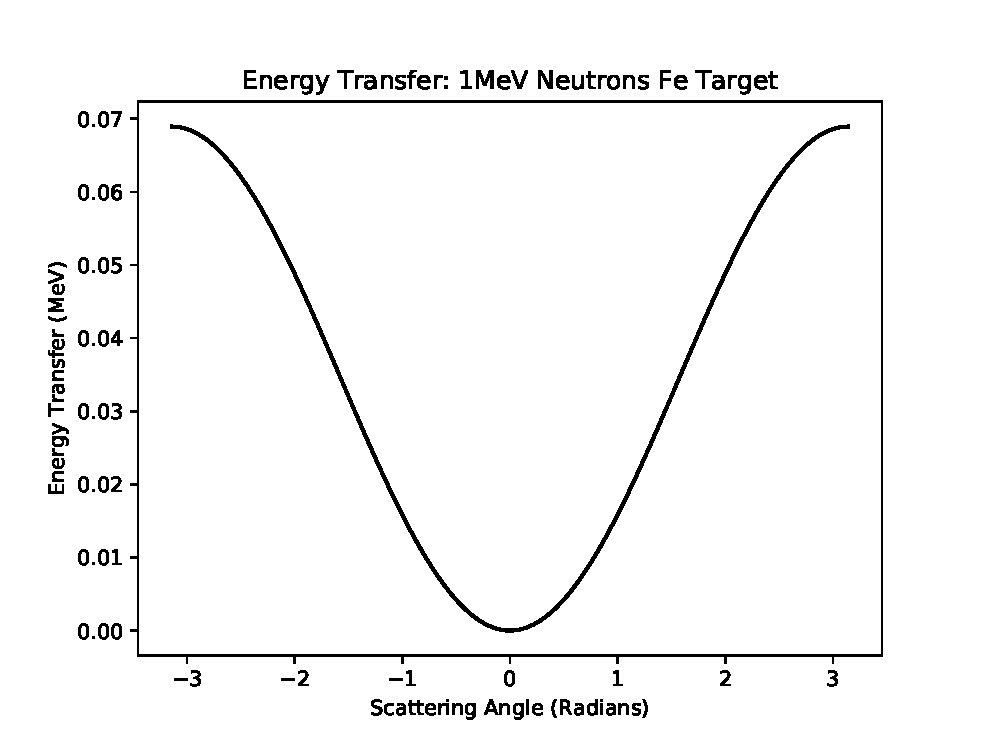
\includegraphics[width=.97\linewidth]{chapters/austenitic_steels_in_nuclear/plots/scattering_angle.eps}
\caption{Scattering angle probability of neutrons plotted with a self written Python script using eq. \ref{eq:eqNeutronEnergyTransfer}\cite{dosimetrygreening}\cite{duderstadthamilton} (elastic scattering only)}
\label{fig:scatteringangle}
\end{minipage}
\begin{minipage}{.01\textwidth}
\end{minipage}
\begin{minipage}{.49\textwidth}
\centering
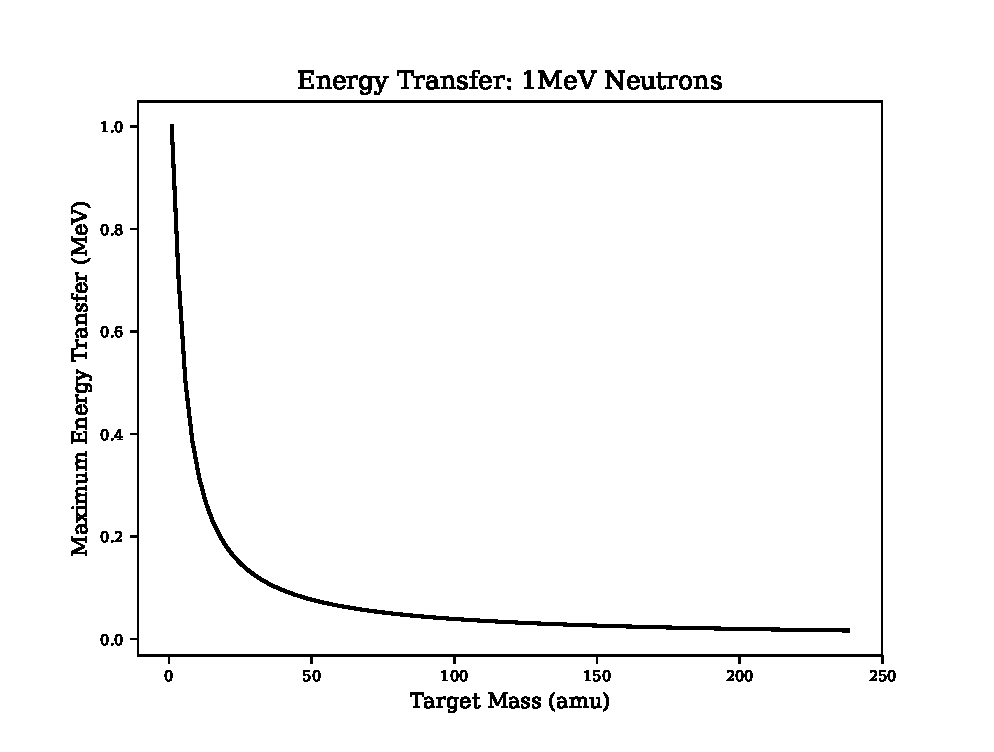
\includegraphics[width=.97\linewidth]{chapters/austenitic_steels_in_nuclear/plots/nuclei_mass.eps}
\caption{Energy transfer as a from a neutron dependant on target mass plotted with a self written Python script using eq. \ref{eq:eqNeutronEnergyTransfer}\cite{dosimetrygreening}\cite{duderstadthamilton} with the scattering angle set to $\pi$ radians, i.e. scattering back and transferring maximum energy to the target nucleus (elastic scattering only)}
\label{fig:energytransfer}
\end{minipage}
\end{figure}

In a collision, the amount of energy transferred to a target atom will depend on both the scattering angle of neutron recoiling from the target and the mass of the target nucleus (fig. \ref{fig:scatteringangle}).  If the neutron does not change direction, a small amount of energy will be transferred, but if it bounces back at 180 degrees it will transfer the maximum amount of energy (fig. \ref{fig:energytransfer}).  A neutron will lose more energy per collision with light atoms (hydrogen, helium, carbon), but much less energy per collision with larger atoms (iron, molybdenum, lead).


The energy of Fe \acrshort{pka}s as a result of neutron irradiation has been calculated for an Fe target\cite{pkaenergyspectra} (fig. \ref{fig:neutronironrecoil}), and those created by 1MeV neutrons may have an energy up to 100keV.  As nuclear reactions are also possible between the neutrons and the target nuclei, there is an inelastic $(n,n) {}^{56}Fe$ channel as well as other elastic scattering channels where the post collision particles are different to the pre collision particles (fig. \ref{fig:ferecoilchannels}).

\begin{figure}[ht]
  \begin{center}
    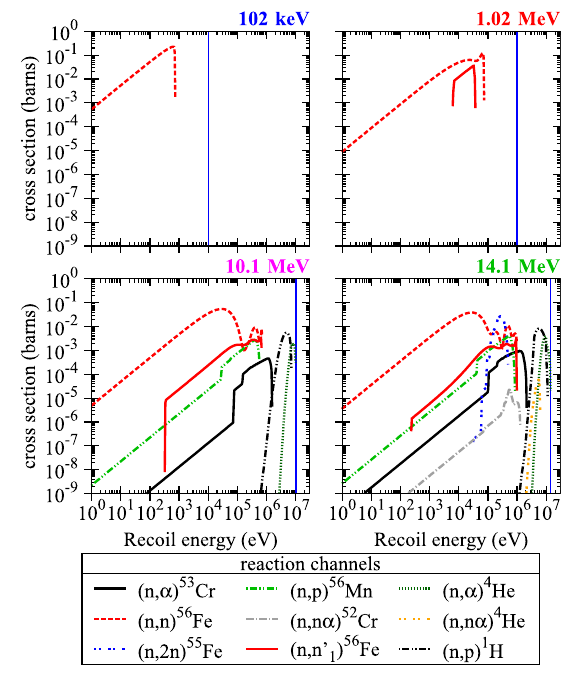
\includegraphics[width=.65\linewidth]{chapters/austenitic_steels_in_nuclear/images/neutronrecoils.png}
    \caption{Recoil energies for neutrons at 102keV, 1.02MeV, 10.1MeV and 14.1MeV\cite{pkaenergyspectra}}
    \label{fig:ferecoilchannels}
  \end{center}
\end{figure}
\FloatBarrier






\FloatBarrier

\subsection{Swelling}

Swelling results from damage to the crystalline structure of the metal and the temperature range for such swelling in steels is primarily from $670K$ to $870K$.  Radiation damage creates a constant supply of Frenkel defects and these take up more volume than the relaxed undamaged crystal.  The vacancies and interstitials may group into prismatic loops of either vacancies or interstitials as these are thermodynamically more stable than the defects being dispersed throughout the crystal\cite{prisloopscnm}.  The creation of vacancy and interstitial loops should balance each other out in terms of the change to the volume, but when the vacancy loops meet in three dimensions they form cavities and these do not decrease the volume of the material\cite{prisloops2}.  The interstitials are the cause for the change in volume, and so the material swells. 

Materials have been known to swell to a 100\% increase in their original volume at these intermediate temperatures under irradiation\cite{wasstrucaustenitic}.  Swelling is sensitive to the total damage amount, the temperature and composition of the alloy.  An increase in Ni decreases swelling as does the addition of Zr.  Small amounts of \Gls{P} and Mo (0.02\% and 0.5-1.0\% respectively) cause the swelling of the alloy to increase, however higher concentrations of either cause swelling to decrease\cite{swellingris}.

As a component swells its properties change.  By definition the volume changes, but so does the elastic moduli.  Not only this, but the swollen component may stress itself and surrounding components, and this may lead to \acrshort{scc}.  Due to the formation of voids and interstitial dislocation networks, stresses are also cause within the material on the microscopic scale.

The swelling of components is a problem experienced in past and current reactors.  In the \acrshort{ebr}-II structural \gls{304SS} was irradiated to 20\acrshort{dpa}.  At a temperature of approximately $650K$ the steel's volume increased by 2\% due to swelling\cite{radisandvoid}.  With components in future reactors expected to withstand ten times this damage, swelling is a concern.  However, increased temperatures and a careful balance in the composition of future alloys will help to reduce this.



\FloatBarrier


\subsection{Radiation Induced Segregation}

The diffusion of atoms within an alloy has an impact on the characteristics of the metal \cite{nickeldiffusion}.  When radiation causes point defects, these interstitials also diffuse parallel to thermal solute diffusion.  At low temperatures, the atoms are unable to diffuse at an appreciable rate; the mobility of vacancies are low\cite{gswas} and there are an excess of vacancies due to radiation damage, and this leads to recombination of defects.  At high temperatures, there is a higher concentration of thermal defects\cite{lightwaterallenbusby}.  This increases the defect recombination rate and reduces migration of defects to sinks, such as grain boundaries.

The melting temperature range of 304 and 316 stainless steel are approximatelyh 1695-1722K and 1644-1672K respectively.  \acrshort{gen2} reactors, such as Sizewell B, have an operating temperature of several hundred degrees centigrade.  The inlet temperature for the Sizewell B PWR reactor is 566K\cite{sizewellbtemp} and the outlet temperature is 597K\cite{sizewellbtemp}.  Operating at approximately 35\% the melting point of the steel this is, unfortunately, a good temperature for \acrfull{ris} to occur.

The \acrfull{ke} concerns the diffusion of one material into another and vice versa at an interface.  In the original experiment performed by Kirkendall and Smigelskas, brass (\Gls{Cu} and Zn) was sandwiched between \Gls{Cu} and left at a temperature of over 1050K for almost two months.  Using \Gls{Mo} as a marker, it was discovered that \Gls{Zn} diffused out of the brass faster than the \Gls{Cu} diffused into the brass.  The flux of atoms results in a flux of defects into and a shrink in volume of the brass\cite{gswasike}.

The \acrfull{ike} is driven by an external force, such as irradiation.  Irradiation of the material causes a flux of defects and, inverse to the \acrshort{ke}, this causes a flux of atoms.  For an austenitic stainless steel the diffusion coefficients in order of size are $D_{Cr} > D_{Fe} > D_{Ni}$\cite{risfecrni}, so Cr will diffuse away from grain boundaries and other sinks, followed by Fe.  As Ni is slowest to diffuse, this will be enriched.  An additional mechanism that is thought to contribute to \acrshort{ris} is interstitial flux where undersized atoms as interstitials are preferential\cite{risfecrni}.

\begin{figure}[ht]
\centering
\begin{minipage}{.46\textwidth}
\centering
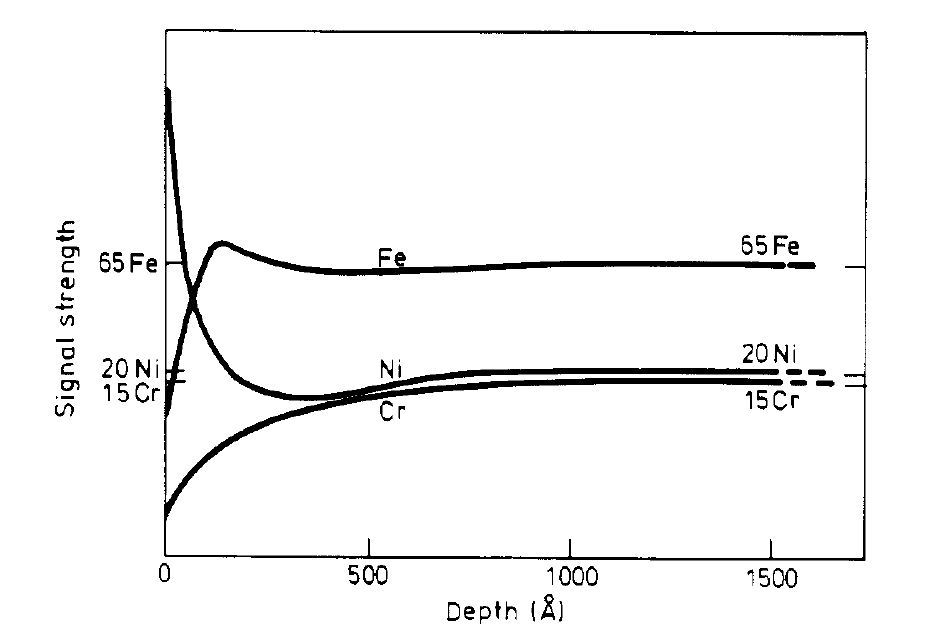
\includegraphics[width=.9\linewidth]{chapters/austenitic_steels_in_nuclear/images/marwickfecrniseg1.png}
\caption{Depletion of cr, fe and enrichment of ni at the surface\cite{johnstonris}}
\label{fig:johnstonris}
\end{minipage}
\begin{minipage}{.05\textwidth}
\end{minipage}
\begin{minipage}{.46\textwidth}
\centering
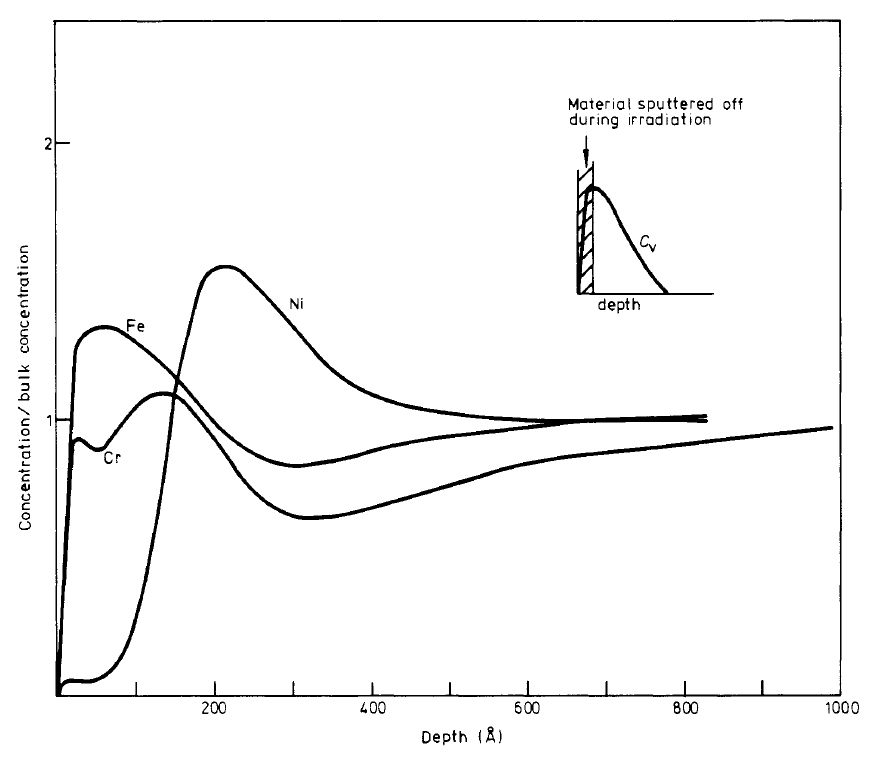
\includegraphics[width=.9\linewidth]{chapters/austenitic_steels_in_nuclear/images/marwickfecrniseg2.png}
\caption{Concentration profile after 46\acrshort{dpa} irradiation with 75 keV Ni ions\cite{marwickris}}
\label{fig:marwickris}
\end{minipage}
\end{figure}

\FloatBarrier

Experimental work by Johnston et al irradiated steel, containing 15\% Cr and 20\% Ni, with 4MeV Ni ions.  It was irradiated to a damage dose of 8\acrshort{dpa} at $950K$.  Some material will have been sputtered from the surface, but in the remaining material Cr, and Fe, were depleted.  Ni, however, was enriched (fig. \ref{fig:johnstonris}).

In work by Marwick a similar alloy with 14\% Cr and 15\% Ni was irradiated to a much higher dose of 46 \acrshort{dpa} with lower energy 75KeV Ni ions.  In this instance the damage occurs in a much thinner layer of the surface that was approximately 30nm thick (fig. \ref{fig:marwickris}).  Conversely to Johnston et al, in this thin layer there is a depletion of Ni and an enrichment of Cr in the first 20nm or so.  However, between approximately 25nm and 60nm there is a similar depletion of Fe and Cr as well as an enrichment of Ni.


\begin{figure}[h]
  \begin{center}
    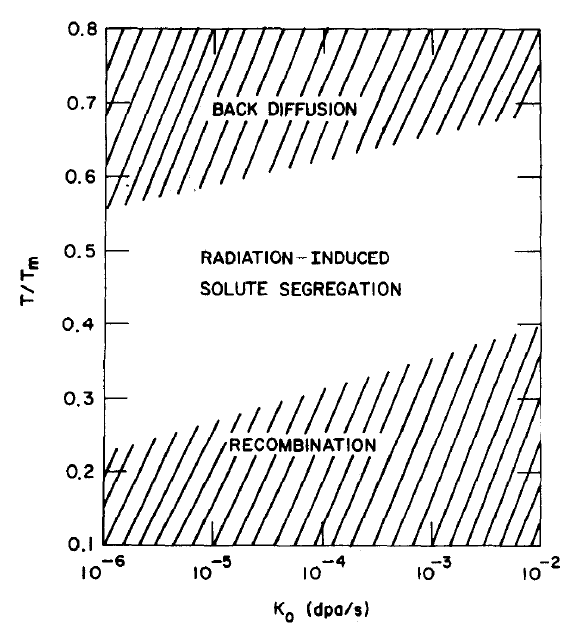
\includegraphics[width=.5\linewidth]{chapters/austenitic_steels_in_nuclear/images/okamoto_rehn_temp_ris.png}
    \caption{Temperature and \acrshort{dpa} dependence of \acrshort{ris}\cite{risokamoto}}
    \label{fig:ristemperature}
  \end{center}
\end{figure}

The underlying mechanisms of \acrshort{ris} are dependent on both the temperature (relative to the melting point of the material) and the amount of damage (fig. \ref{fig:ristemperature}).  The result of \acrshort{ris} is a breakdown in the passive protection of Cr, which leads to \acrshort{igscc} under the correct conditions.


\FloatBarrier

%\begin{figure}[h]
%  \begin{center}
%    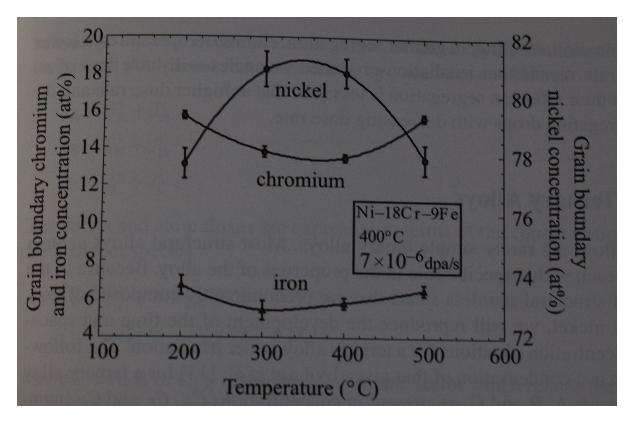
\includegraphics[width=.65\linewidth]{chapters/austenitic_steels_in_nuclear/plots/nicrfeseg.eps}
%    \caption{Grain boundary concentrations at $200^{\circ}C$ to $500^{\circ}C$}
%    \label{graph:grainboundaryconc}
%  \end{center}
%\end{figure}

%\begin{figure}[h]
%  \begin{center}
%    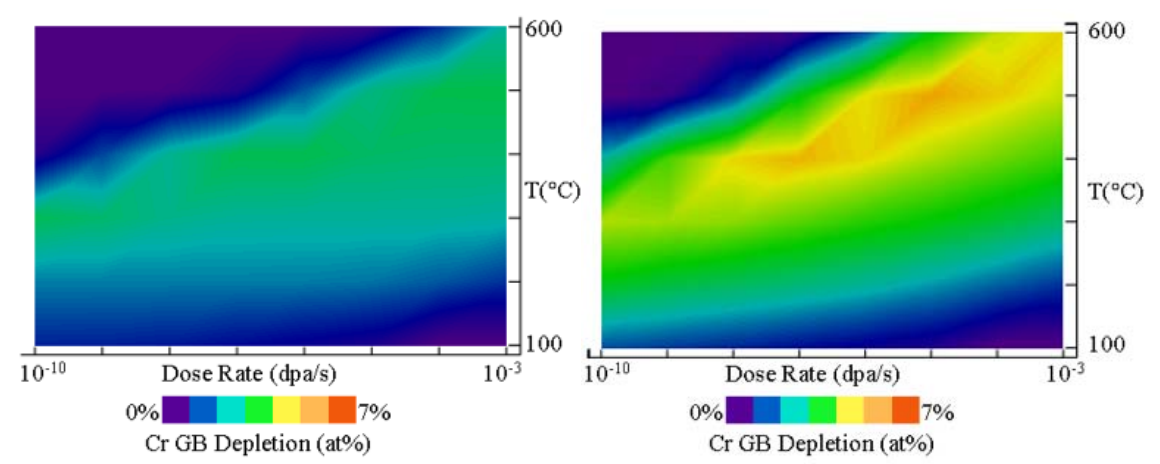
\includegraphics[width=.65\linewidth]{chapters/austenitic_steels_in_nuclear/images/crseg.png}
%    \caption{Chromium grain boundary depletion}
%    \label{graph:crgbdepletion}
%  \end{center}
%\end{figure}



\FloatBarrier





%%%%%%%%%%%%%%%%%%%%%%%%%%%%%%%%%%%%%%%%%%%%%%%%%%%%%%%%%%%%%%%%%%%%%%%%%%%%%%%%%%%%%%%%%%%%%%%%%%%%%%%%%%
%%
%%  Corrosion Resistance
%%
%%%%%%%%%%%%%%%%%%%%%%%%%%%%%%%%%%%%%%%%%%%%%%%%%%%%%%%%%%%%%%%%%%%%%%%%%%%%%%%%%%%%%%%%%%%%%%%%%%%%%%%%%%


\section[Corrosion Resistance]{Corrosion Resistance of Austenitic Stainless Steels}

\subsection{Passive Film Protection of Chromium}

The addition of Cr improves the resistance of stainless steel to corrosion by orders of magnitude.  A very thin passive oxide layer, 20-30 angstroms in width, forms when the surface is exposed to an environment containing \Gls{O}.  The protective layer is self repairing and as such, if the surface is damaged, the oxide layer reforms in the presence of \Gls{O}.

When the steel is in an environment containing \Gls{O}, electrons within the metal tunnel through the surface.  As an oxidizing agent, the nearby \Gls{O} atoms readily accept the electrons.  A strong electric field forms between positive ions within in the metal and the negatively charged \Gls{O} atoms \cite{medicalmetals133}.  

Fe at the surface of the forming oxide layer is preferentially dissolved away over Cr \cite{kirchheimcc} and Cr ions within the oxide layer have a lower mobility than Fe ions \cite{kirchheimpassive}.  Ni remains in place within the alloy, and this leads to an enrichment of chromium oxide in the passive layer.  Once the layer is thick enough to reduce the electric field across it, the formation of the layer stops.  As mentioned previously, this is at a layer thickness of 2-3nm for stainless steel.

The $\text{Cr}_{2}\text{O}_{3}$ layer may be formed by heating the steel to $770K$\cite{propaustenitic}.  However, at higher temperatures, the steel begins to lose its protective layer due to \gls{sensitization}.


\subsection{\Gls{sensitization} and Passive Film Removal}

Steel by definition is Fe alloyed with varying small percentages of \Gls{C}.  The addition of \Gls{C} changes the property of the alloy, and one example of this is an increase in hardness over pure Fe.  At elevated temperatures, 670K to 1020K, the added Cr within the steel forms precipitates of Fe-Cr carbides $(\text{Fe}\text{Cr})_{23} C_{6}$ at the grain boundaries, reducing the percentage of Cr at the grain boundary and removing the layer of passive protection (fig. \ref{fig:alloysensitization1} \& \ref{fig:alloysensitization2}).

\begin{figure}[!h]
\centering
\begin{minipage}{.44\textwidth}
\centering
  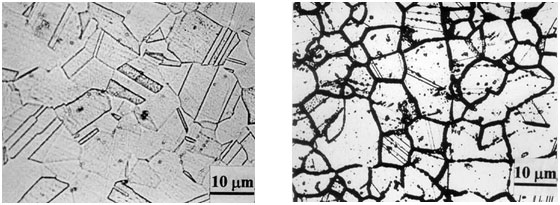
\includegraphics[width=.9\linewidth]{chapters/austenitic_steels_in_nuclear/images/alloy-sensitization.jpg}
  \caption{Formation of chromium precipitates at the grain boundary \cite{rolledalloys}}
  \label{fig:alloysensitization1}
\end{minipage}
\begin{minipage}{.04\textwidth}
\end{minipage}
\begin{minipage}{.44\textwidth}
\centering
  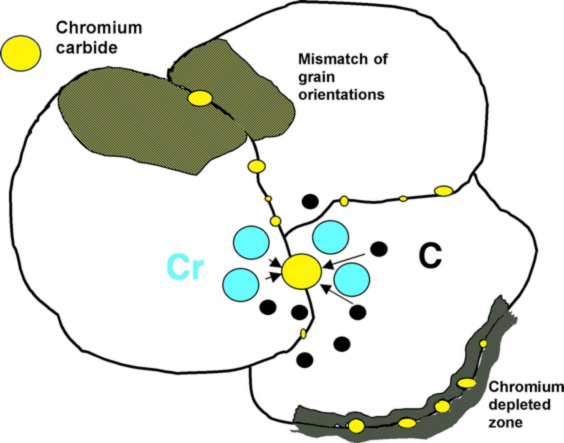
\includegraphics[width=.9\linewidth]{chapters/austenitic_steels_in_nuclear/images/Intergranular-corrosion__figure2.jpg}
  \caption{Sensitization of an alloy: chromium carbide precipitation \cite{ssina}}
  \label{fig:alloysensitization2}
\end{minipage}
\end{figure}

The sensitization of the steel can be reversed.  By heating the steel further, to approximately 1,320K to 1,420K, the steel is solution annealed dissolving the carbides back into the steel.



\subsection{Addition of Molybdenum}

A common austenitic stainless steel is \gls{304SS} and this relies heavily on the passive film due to a high content of Cr, ranging from 17.5\% to 20\% for grades 304, 304L and 304H.  A similar stainless steel, 316, has slightly less Cr, slightly more Ni and 2-3\% Mo, an element not present in 304 stainless steel.

Pure Mo has a \acrshort{bcc} crystal structure, and it is a ferrite former.  However, high proportions of austenite former such as Ni and N force 316 stainless steel to keep its \acrshort{fcc} structure despite the addition of Mo.  Adding it to austenitic steels improves their strength and resistance to creep at high temperatures.  

Steels such as \gls{316SS} are known to have better corrosion resistance in chloride rich environments.  Where at least 2\% Mo has been added it improves resistance to pitting and crevice corrosion resistance\cite{corrosionmo}.  The mechanism by which Mo helps to protect against corrosion is still unclear.  It is possible the addition helps to reduce the breakdown of the passive film protecting the steel, but it may also be the case that Mo promotes the repair of the passive film \cite{moprotection}.














%%%%%%%%%%%%%%%%%%%%%%%%%%%%%%%%%%%%%%%%%%%%%%%%%%%%%%%%%%%%%%%%%%%%%%%%%%%%%%%%%%%%%%%%%%%%%%%%%%%%%%%%%%
%%
%%  Intergranular Stress Corrosion Cracking
%%
%%%%%%%%%%%%%%%%%%%%%%%%%%%%%%%%%%%%%%%%%%%%%%%%%%%%%%%%%%%%%%%%%%%%%%%%%%%%%%%%%%%%%%%%%%%%%%%%%%%%%%%%%%




\section[IASCC]{Irradiation Assisted Stress Corrosion Cracking}

\FloatBarrier

Damage due to irradiation was first identified in high stress stainless steel components in a reactor, such as bolts, springs, and fuel elements\cite{gswasiascc}\cite{iascckenikjonesbell}, and later being found in lower stress austenitic stainless steel components\cite{iascckenikjonesbell}.

\begin{figure}[h]
  \begin{center}
    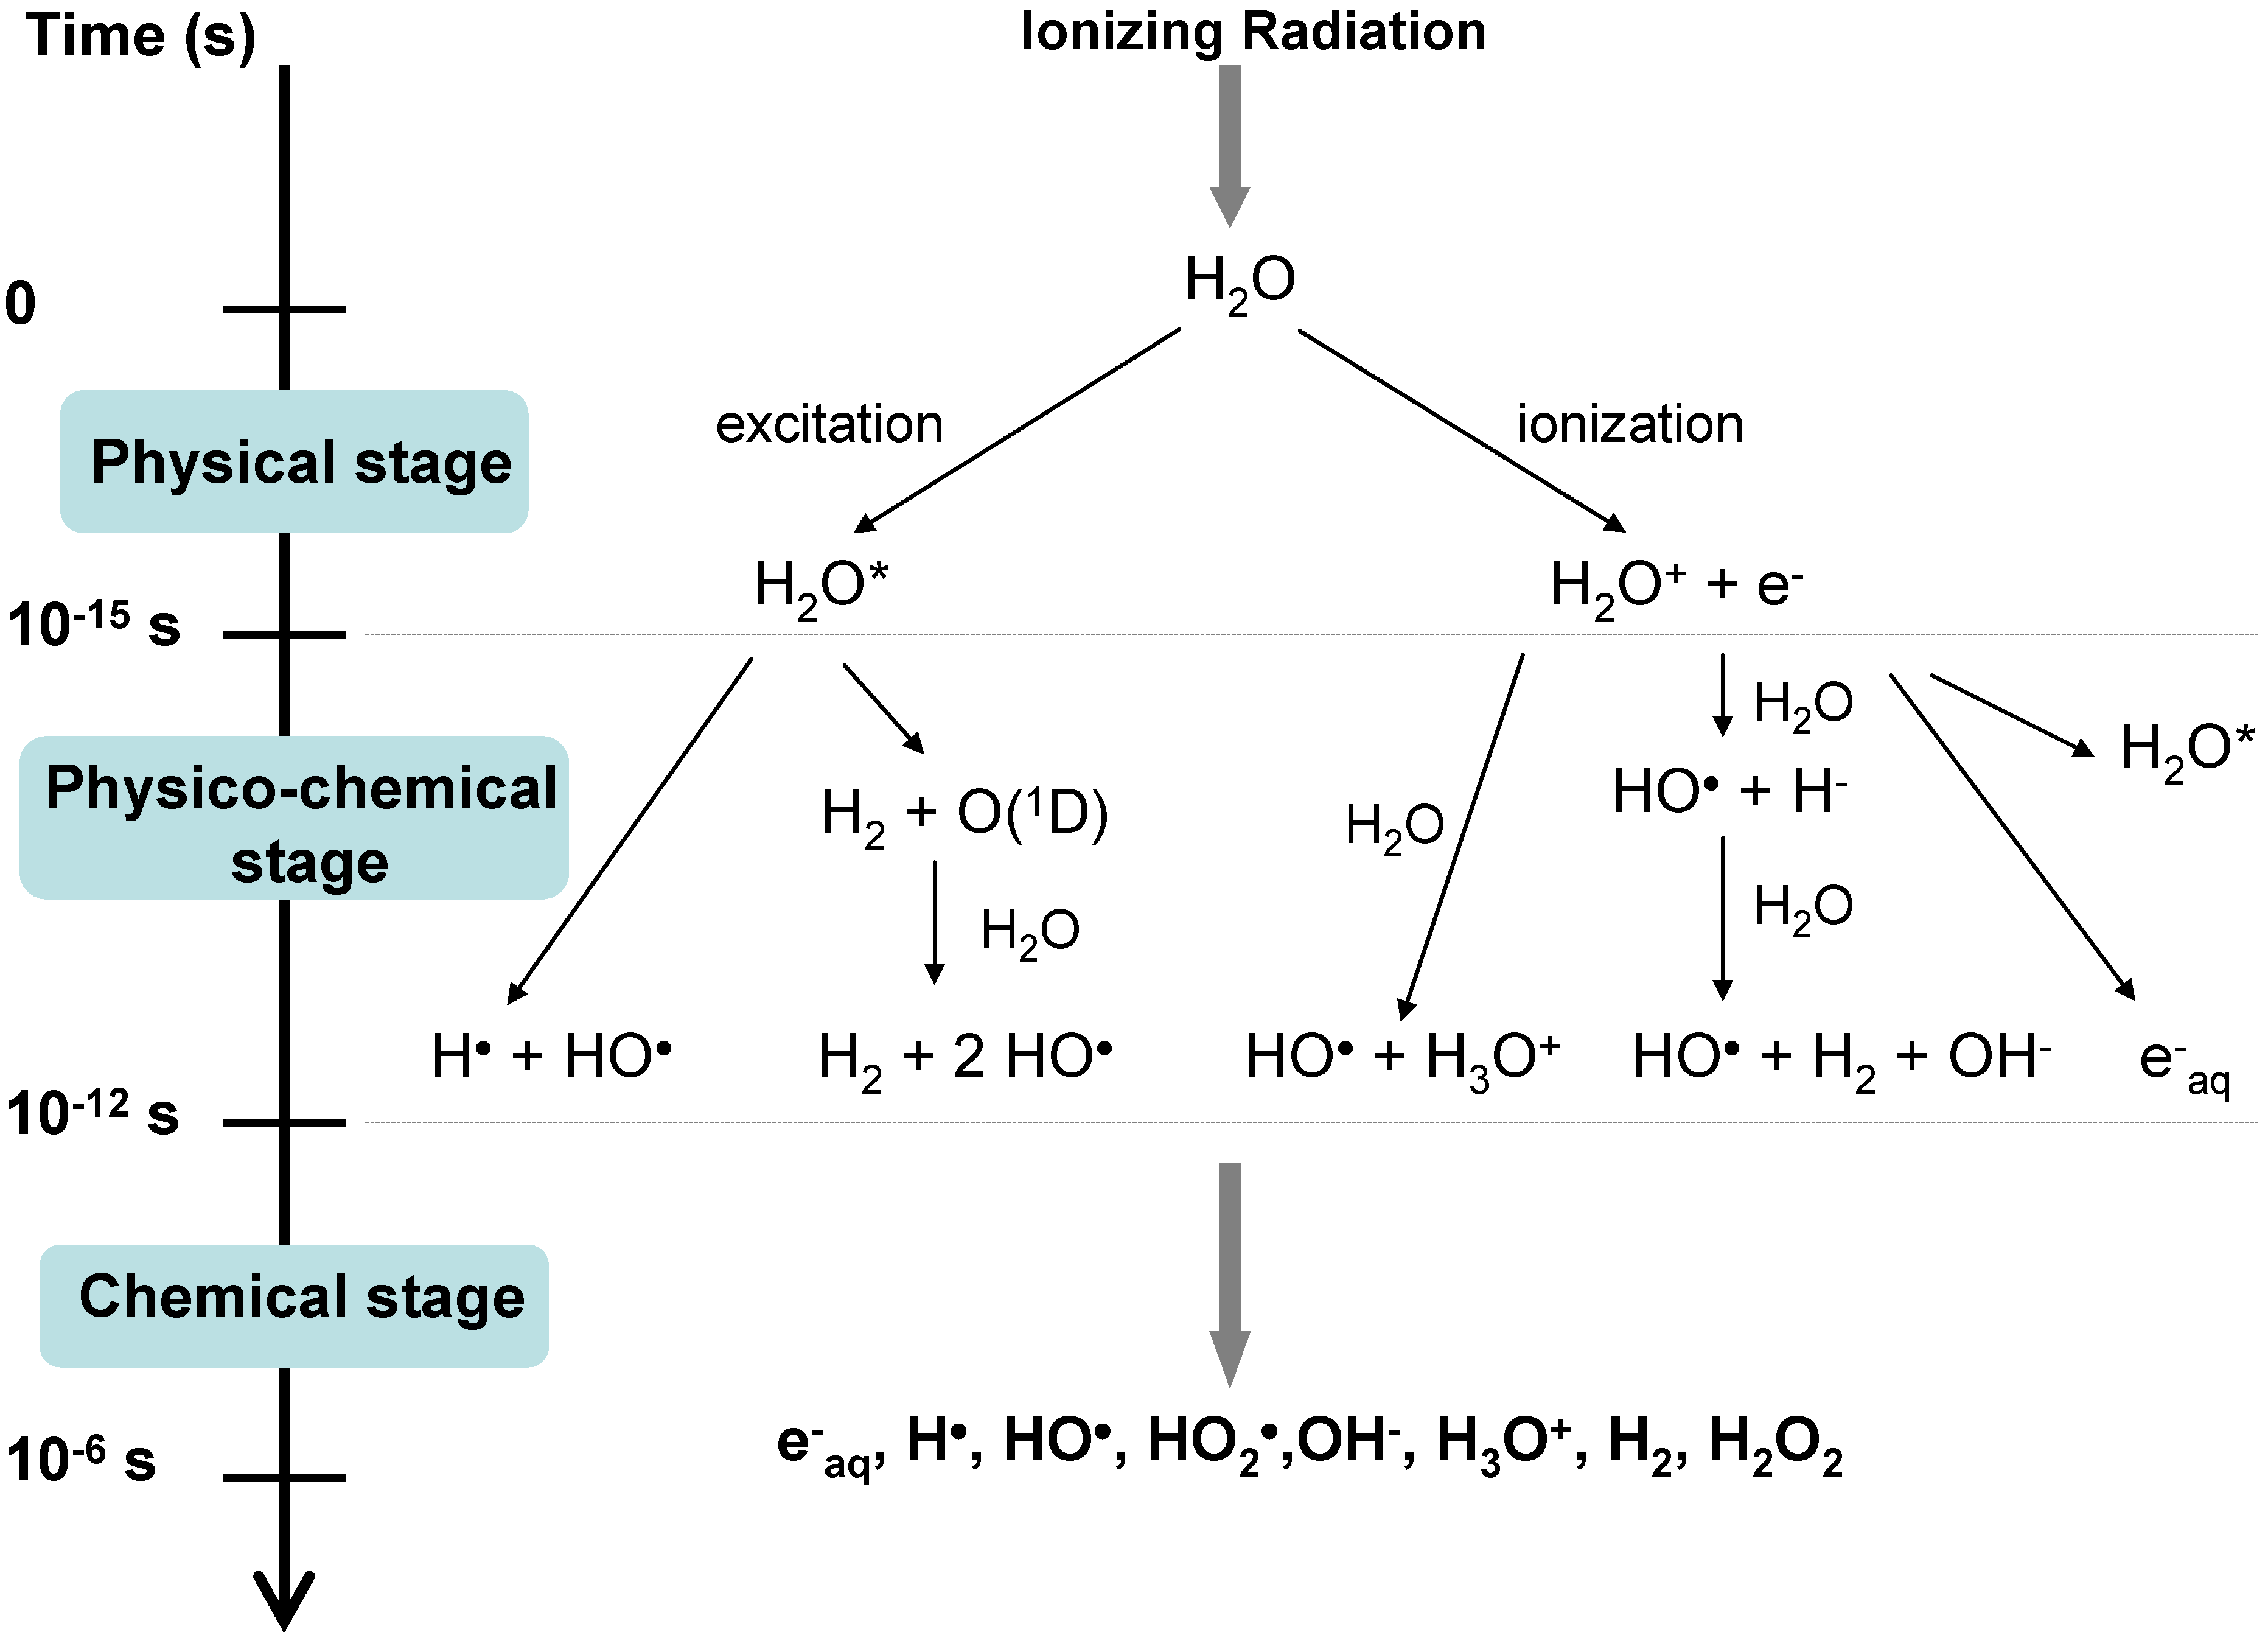
\includegraphics[width=.5\linewidth]{chapters/austenitic_steels_in_nuclear/images/water_radiolysis.png}
    \caption{Changing water chemistry: radiolysis of water\cite{waterradiolysis}}
    \label{fig:radiolysisofwater}
  \end{center}
\end{figure}

Irradiation of water causes the radiolysis of water, changing the chemistry of water and creating hydrogen, radicals and other ions that increase the corrosiveness of the environment (fig. \ref{fig:radiolysisofwater}).  The radiation also damages the material directly, changing its properties.  A form of \acrshort{iascc} to which high nickel alloys, including austenitic steels, are particularly susceptible to is \acrlong{igscc}.


\FloatBarrier

\section[IGSCC]{Inter Granular Stress Corrosion Cracking}

Stress corrosion cracking may be trans granular (through the grains) or inter granular (fig. \ref{fig:igsccni}), at the grain boundary.  \acrshort{igscc} is a particularly prominent failure mechanism for austenitic stainless steels.  For \acrshort{igscc} to occur, there must be a material that is susceptible to this form of cracking, an environment that is corrosive to the material as well as stress (fig. \ref{fig:igsccrequirements}).  

\begin{figure}[h]
  \begin{center}
    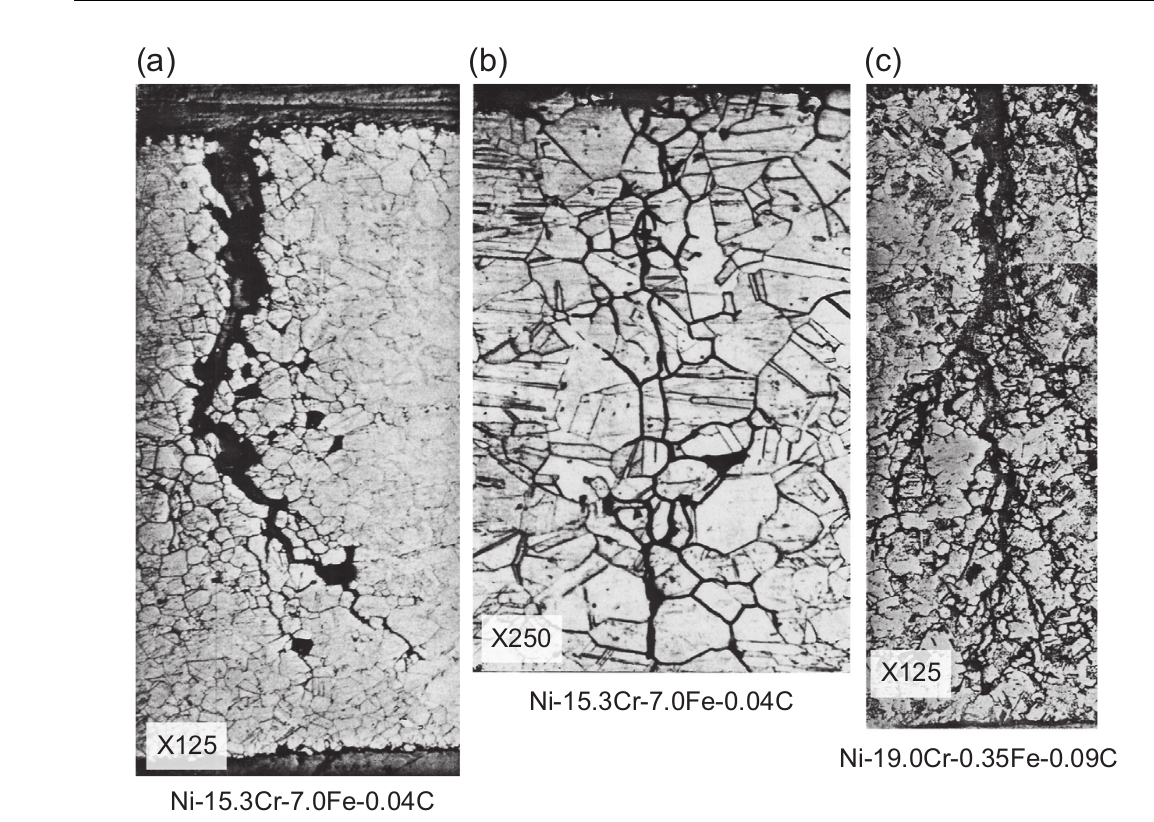
\includegraphics[width=.45\linewidth]{chapters/austenitic_steels_in_nuclear/images/igscc_nickel_alloy600.png}
    \caption{Inter Granular Stress Corrosion Cracking in Nickel Alloy\cite{staehlecoriou}}
    \label{fig:igsccni}
  \end{center}
\end{figure}

Stress may come from a high pressure environment, residual stresses due to welding and swelling.  In a nuclear reactor the swelling on a macroscopic scale is a result of damage caused by neutrons on the atomic scale as they pass through the steel creating defects.  If \Gls{Cr} is depleted at the grain boundary, protection to corrosion due to the passive layer is lost.  This, coupled with the knowledge that austenitic stainless steels are susceptible to \acrshort{igscc}, completes the three requirements and, over time, components of this material in these conditions will eventually fail to \acrshort{igscc}.

\begin{figure}[h]
\begin{center}
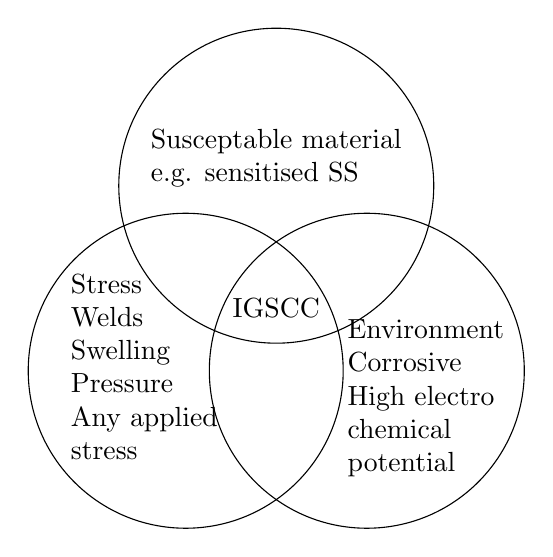
\begin{tikzpicture}[scale=0.50]
\draw (4.5,5.5) circle [radius=4.0];
\draw (2.2,0.8) circle [radius=4.0];
\draw (6.8,0.8) circle [radius=4.0];
\node[align=left] at (4.5, 2.4) {IGSCC};
\node[align=left] at (1.15,0.9) {Stress\\Welds\\Swelling\\Pressure\\Any applied \\stress};
\node[align=left] at (4.5, 6.2) {Susceptable material \\ e.g. sensitised SS};
\node[align=left] at (8.3,0.1) {Environment\\ Corrosive\\ High electro \\chemical \\ potential};
\end{tikzpicture}
\caption{Three requirements for \acrshort{igscc} to occur}
\label{fig:igsccrequirements}
\end{center}
\end{figure}

\acrshort{igscc} has not only been a defect in stainless steel.  High Ni content alloys, such as Alloy 600 (Inconel:  Ni-72, Cr-17, Fe-10),  have been known to suffer from \acrshort{igscc} since the very early days of nuclear energy, in particular with the prototype S1W reactor, prototype for the first nuclear powered submarine, the USS Nautilus.

After the war, there was a drive to develop a nuclear powered navy for the US.  There are obvious benefits in replacing conventional power in vessels with nuclear, in particular for submarines.  This was pushed by Admiral Rickover and the route to building the USS Nautilus began.  A number of available Fe-Cr-Ni alloys were considered for the construction of the reactor (fig. \ref{fig:fecrnialloys}).

\begin{figure}[h]
\centering
\begin{minipage}{.46\textwidth}
\centering
    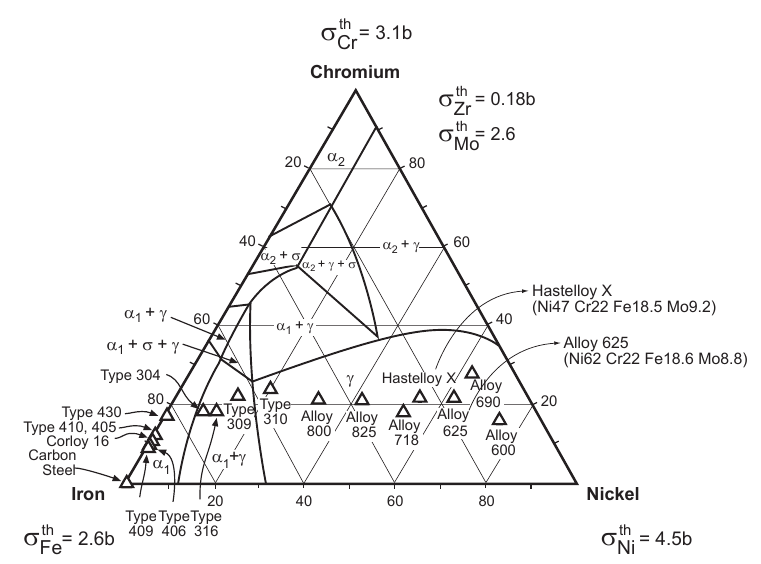
\includegraphics[width=.8\linewidth]{chapters/austenitic_steels_in_nuclear/images/fecrnialloys.png}
    \caption{Alloy choices for early LWRs\cite{staehlecoriou12}}
    \label{fig:fecrnialloys}
\end{minipage}
\begin{minipage}{.05\textwidth}
\end{minipage}
\begin{minipage}{.46\textwidth}
\centering
    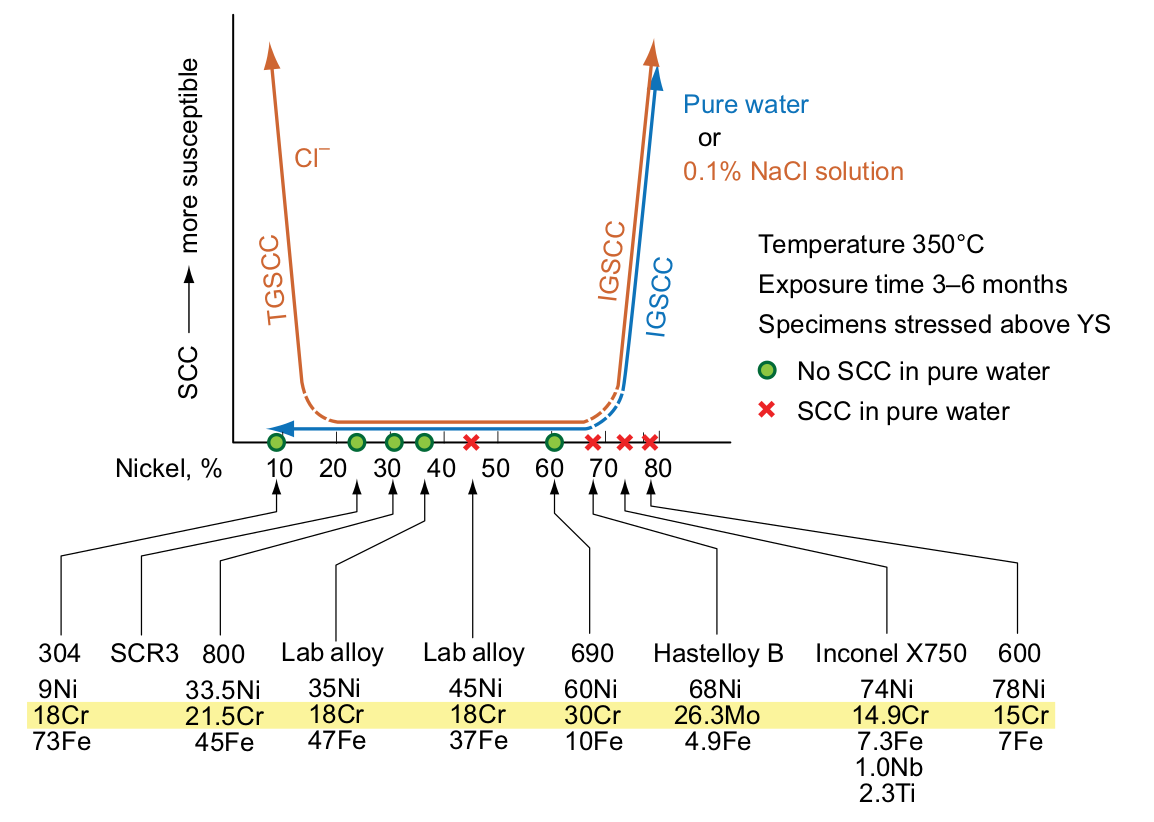
\includegraphics[width=.8\linewidth]{chapters/austenitic_steels_in_nuclear/images/tgscc_igscc_vs_nickel.png}
    \caption{Nickel, IGSCC and TGSCC\cite{staehlecoriou15}}
    \label{fig:nitgsccigscc}
\end{minipage}
\end{figure}

Prototypes developed for the USS Nautilus experienced stress corrosion cracking in the Inconel Alloy 600 components.  H. Coriou replicated this damage to Inconel in the laboratory, holding a sample at $620K$ in deoxygenated water for 3 months\cite{staehlecoriou}.  Further studies showed that \acrshort{igscc} became a particular issue to alloys with a high Ni content in pure water, commencing with a content of approximately 70\% Ni.  In a weak salt water solution (0.1\% NaCl) \acrshort{igscc} occurred as with the same alloy in pure water, but \acrshort{tgscc} occurred in similar alloys with a low Ni content (less that 15\%) (fig. \ref{fig:nitgsccigscc}).


\FloatBarrier

\subsection{IGSCC in Light Water Reactors}

In \acrshort{lwr}s a major factor in corrosion of components is the water chemistry and \acrlong{ecp} that they operate in.  Higher levels of oxygen dissolved in the water leads to an increase in the corrosion potential\cite{wasstrucaustenitic}.  Other factors within \acrshort{lwr}s include depletion of \Gls{Cr} due to either heat treatment, welding or irradiation.

The primary circuit of a \acrshort{bwr} includes components such as a reactor pressure vessel, piping that leads out of the containment building, fuel and fuel assembly.  300 series steels, including 304 and 316, are used within the primary circuit, including the piping and control rod absorbers.  In \acrshort{bwr}s the purity of the water has been addressed, and the addition of hydrogen to the water has reduced cracking of components\cite{staehlecoriou}.  

Higher nickel content steels such as the 600 series alloys are used in \acrshort{pwr}s, and components that are made from these alloys include steam generators and pressure vessels.  In the AP-1000 design, the control rod drive mechanism at the reactor coolant pressure boundary are made from 304, 304L, 304LN, 316, 316L and 316LN steel.  Higher nickel content 690 is used for penetration into the pressure vessel\cite{ap1000dcd}.  As illustrated by Coriou's work in the 1950s and 1960s, higher nickel content steels are susceptible to \acrlong{scc}.

\FloatBarrier
\subsection{IGSCC and Advanced Gas-cooled Reactors}

A major drawback of the first generation Magnox reactors was their relatively low operating temperature of $630K$.  Carnot's theorem shows that the maximum amount of energy from an engine is dependent on the difference between the hot and cold reservoirs (section \ref{section:carnottheorem}).  The ambient temperature of the power station will vary a small amount with the seasons.  The practical way to improve the maximum possible efficiency is to increase the engine (reactor) temperature.

\acrshort{agr}s were designed to run at much higher temperatures of $920K$.  By increasing the temperature, the maximum possible thermal efficiency was increased from just over 50 percent to almost 70 percent.  To withstand higher temperatures, the magnesium oxide cladding used in the earlier Magnox reactors was replaced with stainless steel.  To counteract the higher neutron absorption cross section of the cladding, the fuel was enriched up to 3.5\% $\text{U}^{235}$.

The cladding holds the fuel elements together and at the required location inside the reactor whilst it is consumed in the reactor.  The cladding also performs several functions once the fuel has been spent.  It holds the fuel elements together and acts as a primary containment for the spent fuel\cite{agrfuelstorage}.

During its lifetime as a fuel element within the reactor, the cladding has been heated and irradiated.  By the process of \acrshort{ris} the Cr at the grain boundary can drop to 10\% concentration\cite{agrigscc}.  The C rich environment within the reactor, due to the $\text{CO}_{2}$ coolant, provides yet another mechanism to deplete Cr at the grain boundary by the formation of Fe-Cr carbides $(\text{Fe}\text{Cr})_{23} C_{6})$.  

This loss of protection at the grain boundary, stress due to the role of the component within the reactor, the changing environment due to radiation damage and the material's susceptibility lead to \acrshort{igscc}.




\FloatBarrier



\section[SS in Gen III+ and Gen IV]{Austenitic Stainless Steels in Gen III+ and Gen IV Reactors}

The AP1000 is an advanced \acrshort{pwr}.  As a Westinghouse reactor, the fuel cladding will be their trademarked Zirlo alloy.  Inconel will be used for the steam generator and heat exchanger with carbon steel used for the construction of the pressure vessel.  The control rod absobers, however, will be constructed from \gls{304SS}\cite{ap1000mat}.

Areva designed the EPR and this will use \gls{316SS} as the fuel cladding material.  It will also use the slightly less corrosion resistant \gls{304SS} (forged) in parts of the control rod drive mechanisms\cite{eprmat}.

The perforated upper core plate, between the reactor core and the inlet/outlet/control rod mechanisms, is also made from austenitic stainless steel.  The pressuriser is constructed from ferritic steel, but its internals are clad with austenitic stainless steel to protect the structure from the coolant.

\acrshort{gen4} designs also include the use of austenitic stainless steels.  Experimental fast reactors in many countries, including the US, UK, Japan, France, India and China have used either \gls{304SS}, \gls{316SS} or both in their construction.

Austenitic steels are more corrosion resistant than ferritic or martensitic steels.  They do expand more as a result of being irradiated, but they are stronger at higher temperatures.  Many of the \acrshort{gen4} reactors operate at much higher temperatures than existing reactors and the components will be expected to resist higher doses of radiation damage throughout their lifetime.

\acrshort{gfr}s are expected to use austenitic steels.  Due to their chemical compatibility with sodium they are also expected to be used in \acrshort{sfr}s.  As well as being used in the reactor core, these steels will also be used outside the core.  For example, \acrshort{sfr}s in France will use austenitic steels in the secondary circuit, primary pump, internal heat exchanger and more\cite{convsteelooc}.


\FloatBarrier



\section[Addition of PGMs]{The Addition of PGMs to Stainless Steel}

Water purity is a concern for light water reactors.  The fewer contaminants there are to begin with, the better.  Even so, the radiolysis of the purest water will still create a steady supply of corrosive molecules (fig. \ref{fig:radiolysisofwater}).  Adding hydrogen to the water reduces the \acrlong{ecp} of the water, but if too much is added it will combine with the radioactive nitrogen-16 created by the ${}^{16}O(n,p){}^{16}N$ reaction to form ${}^{16}NH_{3}$\cite{noblemetalchemical}.

Cathodic modification is a technique used to improve corrosion resistance, and one way to do this for stainless steel is to add small amounts of \acrfull{pgm}s\cite{potgieter1994}.  By adding such metals, the anodic reaction may be reduced.  \acrshort{pgm}s also act as a catalyst in the reduction and removal of $O_2$ and $H_2O_2$ from the water\cite{noblemetalchemical}.

The increased corrosion resistance is dependant upon the amount of \acrshort{pgm} added, but a higher percentage does not necessarily mean better protection.  This is important for two reasons, to find the optimum amount for the sake of corrosion resistance, and to keep the price down as the additions are so expensive, even in such small amounts.

\begin{figure}
\centering
\begin{minipage}{.47\textwidth}
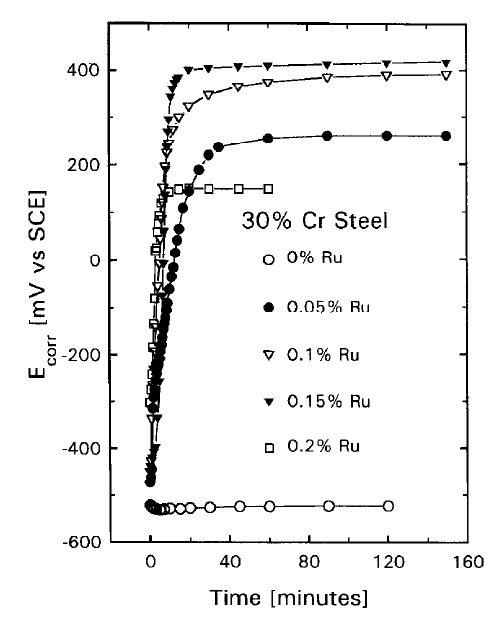
\includegraphics[width=.97\linewidth]{chapters/austenitic_steels_in_nuclear/images/fe30crru.png}
\end{minipage}
\begin{minipage}{.47\textwidth}
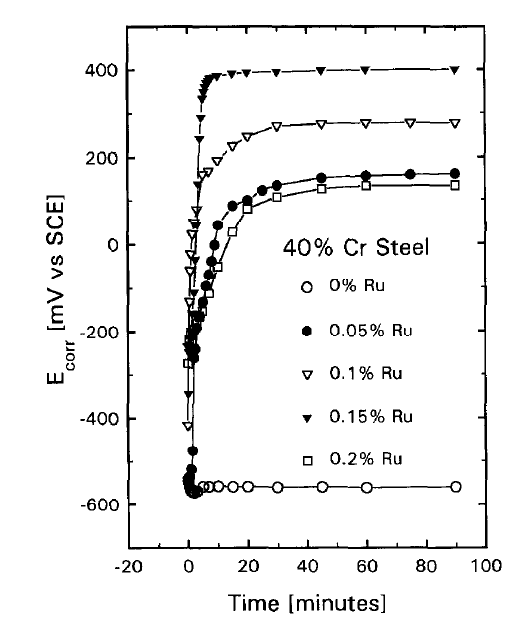
\includegraphics[width=.97\linewidth]{chapters/austenitic_steels_in_nuclear/images/fe40crru.png}
\end{minipage}
\caption{Addition of Ru to Fe30Cr and Fe40Cr steels - open current corrosion potential variation with time in 10\% sulphuric acid\cite{potgieter1994}}
\label{fig:ruadditions}
\end{figure}

It was found that an addition of 0.15\% \Gls{Ru} (out of a selection of 0\%, 0.05\%, 0.10\%, 0.15\% and 0.20\%) was optimum for both Fe30Cr and Fe40Cr steel (fig. \ref{fig:ruadditions})\cite{potgieter1994}.  Other \acrshort{pgm}s may be used for cathodic modification, including \Gls{Pd}, \Gls{Ir} and \Gls{Pt}, but the cost of the metal must be weighed against the possible gains.

\begin{figure}
\centering
\begin{minipage}{.80\linewidth}
\centering
    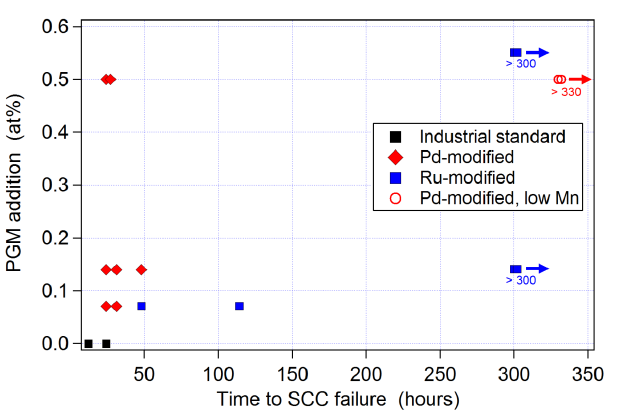
\includegraphics[width=.95\linewidth]{chapters/austenitic_steels_in_nuclear/images/pgmfailure.png}
    \caption{Failure times for 304SS, Pd doped 304SS (with and without Mn) and Ru doped 304SS in polythionic acid at ambient temperature\cite{scrstainless}}
    \label{fig:pgmfailuretimes}
\end{minipage}
\end{figure}

Connolly et al added Ru and Pd to \gls{304SS} samples that were sensitized at 920K for 24 hours\cite{scrstainless}.  After sensitization, the steel was analysed by \acrshort{tem} and Cr-rich carbides were found at grain boundaries.  Without the passive protection due to Cr, the samples were exposed to polythionic acid to promote \acrshort{scc}.  The Ru doped steels performed well, but the Pd doped steels showed no improvement over regular 304SS.  Further analysis of the samples by \acrshort{tem} reveals that the low percentage of Mn in the steel allows the formation of Pd-Mn precipitates at the grain boundary\cite{scrstainless}.  These precipitates form during the sensitization procedure and thus negate the protection by cathodic modification at the surface of the metal by removing the Pd.

With a low Mn 304SS (less than 0.05\% Mn), varied amounts of Pd have been tested.  With the reduction in Mn the corrosion resistance improves greatly over regular 304SS.  Palladium remains at the surface, as the amount of Mn is too low for appreciable amounts of Pd to be lost to precipitate formation during sensitization.  No failures have been observed with either the Ru or Pd (low Mn) samples for 330 hours exposure to polythionic acid at ambient temperatures (fig. \ref{fig:pgmfailuretimes}) \cite{scrstainless}.

The surface of the metal does not need to have a full coating of \acrshort{pgm} but it should be equally spaced across the surface.  Oxidant in the layer at the surface will be consumed at the locations of \acrshort{pgm}s and the change in concentration at those points will naturally cause diffusion of more oxidant to those locations\cite{noblemetalchemical}.

The \acrshort{pgm}s may be coated on the surface of the metal or alloyed to the metal.  The first method is the more cost efficient but if a crack does form, or if a layer is removed, it will expose the regular alloy underneath.  If the \acrshort{pgm} is alloyed, there will always be protection, unless a mechanism is removing the \acrshort{pgm} from the surface.  This could be through precipitation as a carbide, or it could be due to radiation causing the metals to segregate.

\begin{table}[h]
\begin{center}
\renewcommand{\arraystretch}{1.2}
\begin{tabular}{c c}
\hline\hline
Reaction & Product Halflife\\
\hline\hline
${}^{54}Cr(n, \gamma){}^{55}Cr$ & 3.5 mins \\ 
${}^{64}Ni(n, \gamma){}^{65}Ni$ & 2.5 hrs  \\
${}^{55}Mn(n, \gamma){}^{55}Mn$ & 2.6 hrs  \\
${}^{104}Ru(n, \gamma){}^{105}Ru$ & 4.4 hrs  \\
${}^{108}Pd(n, \gamma){}^{109}Pd$ & 13.7 hrs  \\
${}^{196}Pt(n, \gamma){}^{197}Pt$ & 19.9 hrs  \\
\hline\hline
\end{tabular}
\end{center}
\caption{Radioactive products and their half lives for \acrshort{pgm} doped 304SS}
\label{table:304ssradioactive}
\end{table}

Adding elements to metals, even in small amounts, may be problematic as certain elements have high neutron reaction cross sections and transmute into radioactive isotopes.  ${}^{55}Cr$ is a concern for all neutron irradiated stainless steels, but with a very short half life it quickly cools and becomes less of a concern, with ${}^{65}Ni$ becoming the dominant source of activity after 10 hours.  Adding Mn to steel that is in a reactor is known to result in an increase in activity due to the ${}^{55}Mn(n, \gamma){}^{56}Mn$ reaction.  

The addition of \acrshort{pgm}s alters the activity of the steel following neutron irradiation and with just a 1\% addition there is an increase in activity comparable to that of the 10\% Ni transmuted to ${}^{65}Ni$.  This is due to reactions that create ${}^{105}Ru$, 
 ${}^{109}Pd$ and ${}^{197}Pt$ for Ru, Pd and Pt respectively (table \ref{table:304ssradioactive}).  

With such small additions required for cathodic modification and the short half lives of the radioactive isotopes, there isn't a concern due to neutron activation over regular 304SS, and much less of a concern than that of 304SS containing Mn. 






\chapter[Isotope Activation and Radioactive Decay]{Isotope Activation and Radioactive Decay}

\begin{changemargin}{1.0cm}{1.0cm}
\abstractpreamble{Using a proton source is an attractive alternative to neutron sources as they can generate similar damage doses at a much smaller cost.  Isotopes in a material may be transmuted through either neutron or ion irradiation, so this remains a concern.  The probability of transmutation is modelled using the \acrshort{omp} and this data is available in \acrshort{endf}.\\
\\
Radioactive isotopes take time to decay to safe levels, and the chain they follow may be complex.  Bateman developed an equation to model this.  This equation is developed further in chapter \ref{chapter:activitycode} resulting in a code called Activity.  This couples the new equation with cross section data and ion trajectories from \acrshort{trim} and \acrshort{srim}.\\
\\
In this work radiation activation will be modelled and potentials developed to model radiation damage.  This chapter outlines experimental sources of ions and neutrons followed by a discussion of activation and the ion transport codes \acrshort{srim} and \acrshort{trim}.
}
\end{changemargin}




%%%%%%%%%%%%%%%%%%%%%%%%%%%%%%%%%%%%%%%%%%%%%%%%%%%%%%%%%%%%%%%%%%%%%%%%%%%%%%%%%%%%%%%%%%%%%%%%%%%%%%%%%%
%%
%%  Ion Sources
%%
%%%%%%%%%%%%%%%%%%%%%%%%%%%%%%%%%%%%%%%%%%%%%%%%%%%%%%%%%%%%%%%%%%%%%%%%%%%%%%%%%%%%%%%%%%%%%%%%%%%%%%%%%%

\section{Ion Sources}

\subsection{\acrshort{linac}}

Since the development of the first \acrfull{linac} in the 1940s, their modern day versions have become some of the most powerful accelerators in the world.  The longest \acrshort{linac}, \acrlong{slac}, is 3.2km in length and it accelerates electrons and positrons at energies of up to 50GeV.  Several \acrshort{linac}s for protons include the 800MeV \acrshort{linac} component of the ISIS neutron source in Oxfordshire, and the 800MeV \acrshort{linac} used by the \acrlong{sns} at Oak Ridge National Laboratory.

The accelerator is constructed of several tubes, connected alternately to opposite terminals of a high frequency alternating current supply.  As protons enter the first tube, a negative voltage is applied.  As the protons reach the gap between the first and second tube, the polarity is reversed.  The positive charge that is now applied to the first tube pushes the protons forward as the negative charge on the second tube pulls the protons forward.  This process is repeated along the length of the accelerator, with the sections increasing in length due to the increase in velocity of the protons.




\FloatBarrier
\subsection{Cyclotron}

Cyclotrons are reasonably compact and cost effective.  The largest current cyclotron, \acrlong{triumf}, is located in Canada and is able to output protons with energies over 500MeV.  It is relatively large, weighing 170 tons.  There are approximately 350 cyclotrons\cite{cyclotrons} around the world today.

The University of Birmingham cyclotron is more compact.  The protons it accelerates are in the 8-40MeV range and the projectiles are not just restricted to protons (table \ref{table:mc40projectiles}).


\begin{table}[h]
\begin{center}
\renewcommand{\arraystretch}{1.2}
\begin{tabular}{c c c c}
\hline\hline
Projectile & Energy (MeV) & Maximum Current (micro A) & Projectiles $cm^{-2} s{-1}$\\
\hline\hline 
proton & 8-40 & 60 & $5.85 \times 10^{14}$  \\
deuteron & 8-40 & 30 & $2.93 \times 10^{14}$  \\
$He^{2+}$ & 8-53 & 30 & $2.93 \times 10^{14}$ \\
\hline\hline
\end{tabular}
\end{center}
\caption{University of Birmingham Cyclotron Ion Beams.  The projectiles per area is based on a 0.8cmx0.8cm beam aperture.}
\label{table:mc40projectiles}
\end{table}

The moderate size, energy range, availability and cost of these Cyclotrons make them ideal candidates for damaging targets with light ions, rather than neutrons from a neutron source.



\begin{figure}[ht]
\begin{center}
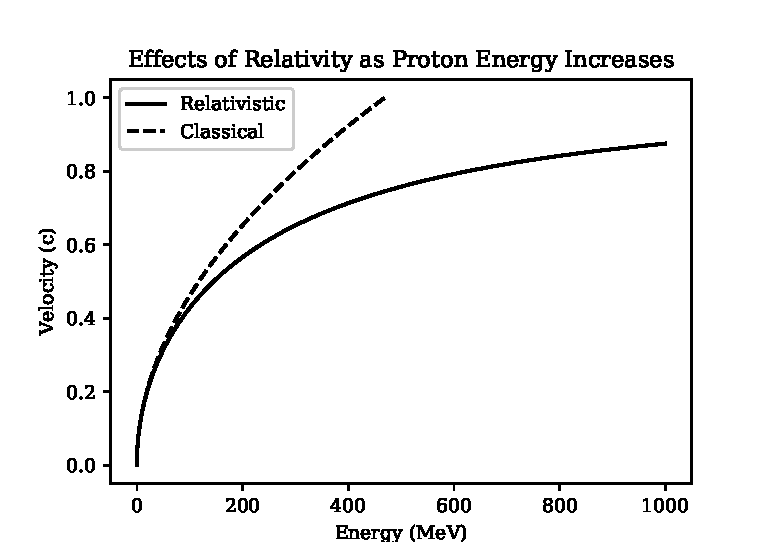
\includegraphics[width=.50\linewidth]{chapters/isotope_activation_and_radioactive_decay/plots/relativistic/proton_energy.eps}
\captionsetup{font={it}}
\caption{A plot of relativistic and classical velocities for 0MeV - 1000MeV protons}
\label{fig:relitavisticplot}
\end{center}
\end{figure}

The Scanditronix MC40 is an isochronous cyclotron.  As the ions are accelerated to higher and higher velocities, the effects of special relativity become appreciable.  The relativistic velocity ($v$) is dependent upon the speed of light (c), the rest energy of the ion ($E_0$) and the kinetic energy of the particle ($E_t$).  The rest energy is defined by the rest mass ($m_0$) and the speed of light, although the particle rest masses are typically given in energies of MeV.  The difference between the classical and relativistic calculations is illustrated in fig. \ref{fig:relitavisticplot}.

\begin{equation}
\begin{split}
E_0 = m_0 c^2 \\
E_T = m_0 c^2 \left[\frac{1}{\sqrt{1-\frac{v^2}{c^2}}} - 1 \right] \\
\therefore v = c \sqrt{1 - \left(\frac{E_{0}}{E_t + E_{0}}\right)^2}
\end{split}
\label{eq:eqGammaFunction}
\end{equation}

The cyclotron has two Dees and these are D shaped hollow electrodes.  Ions enter at the center of the cyclotron and are held in the Dees as they are accelerated.  The magnetic field is varied to bend the path of the ions from a circle into a round cornered triangle.




\FloatBarrier
\subsection{Synchrotron}

Two of the most well known accelerators are Synchrotrons: the \acrlong{lhc} at \acrlong{cern}, and the now retired Tevatron at Fermilab.  These are typically large machines and there are approximately 70 around the world\cite{synchrotrons}, approximately a fifth the number of Cyclotrons.  

Synchrotrons are used for storing high energy particles in a continuous loop, either to generate light through magnetobremsstrahlung, or for high energy collisions.  Cyclotrons are more commonly used for lower energy (tens of MeV) projectiles, in materials science for damaging materials and for medical use (creating radioactive isotopes for use in hospitals).










%%%%%%%%%%%%%%%%%%%%%%%%%%%%%%%%%%%%%%%%%%%%%%%%%%%%%%%%%%%%%%%%%%%%%%%%%%%%%%%%%%%%%%%%%%%%%%%%%%%%%%%%%%
%%
%%  Neutron Sources
%%
%%%%%%%%%%%%%%%%%%%%%%%%%%%%%%%%%%%%%%%%%%%%%%%%%%%%%%%%%%%%%%%%%%%%%%%%%%%%%%%%%%%%%%%%%%%%%%%%%%%%%%%%%%


\FloatBarrier
\section{Neutron Sources}

\FloatBarrier
\subsection{High-Flux Neutron Reactors}

There are 250 or so research reactors in 55 countries \cite{researchreactorstats}, and a number of these are used for materials research.  In the UK, there is only one remaining research reactor, and this is the Neptune pool type reactor at Rolls Royce\cite{neptunereactor}.  In Cadrache, France, the Jules Horowitz reactor is under construction and this is being built specifically as a materials testing reactor.  It will be crucial in researching new materials for use in upcomming Gen IV nuclear power stations \cite{researchreactorstats}.  


\FloatBarrier
\subsubsection{\acrlong{hfir}, Oak Ridge}

The \acrlong{hfir}, at the \acrlong{ornl} in America, is an 85MW research reactor that provides testing space within the reactor as well as a number of neutron beam lines (fig. \ref{fig:hfir}).  The reactor uses highly enriched Uranium as its fuel source and is scheduled to operate at 100\% capacity for 161 days per year, in cycles of approximately 23 days.  A 30cm surround of Beryllium is used to reflect neutrons, and in the reactor core there is a high flux of thermal neutrons at a rate of $2.3 \times 10^{15}$ neutrons $cm^{-2} s^{-1}$\cite{hfirornluserguide}.


\begin{figure}[ht]
\centering
\begin{subfigure}{.44\textwidth}
  \centering
    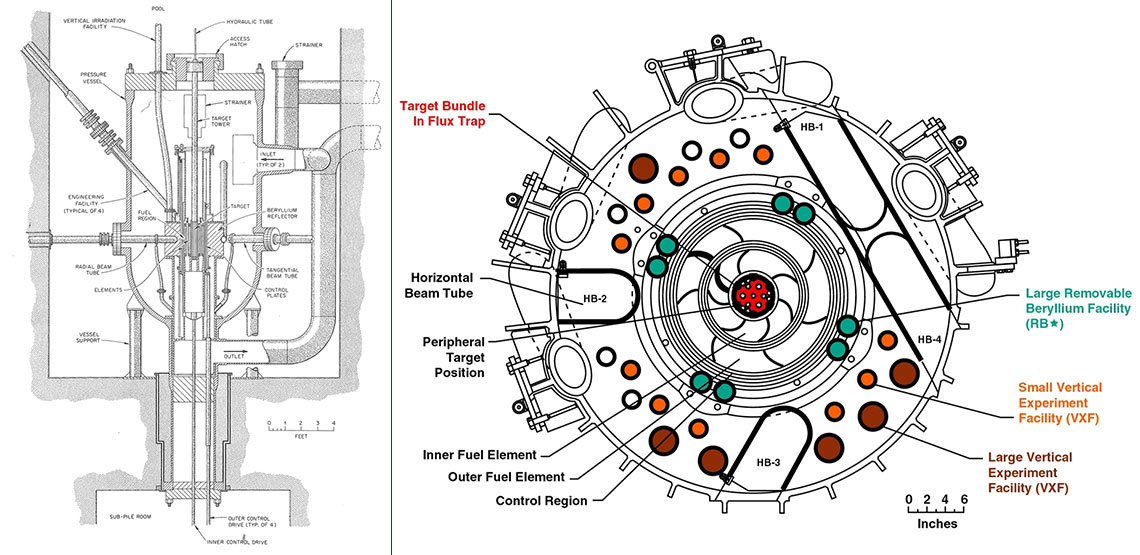
\includegraphics[width=.98\linewidth]{chapters/isotope_activation_and_radioactive_decay/images/hfir-cross-sections.jpg}
    \captionsetup{font={it}}
    \caption{A cross section of the reactor\cite{hfirornl}}
    \label{fig:hfirxs}
\end{subfigure}
\begin{subfigure}{.44\textwidth}
  \centering
    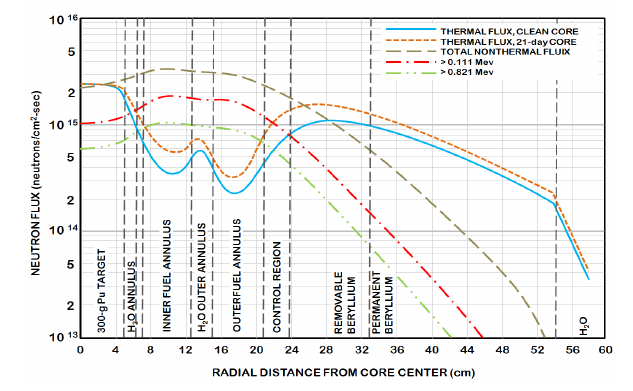
\includegraphics[width=.98\linewidth]{chapters/isotope_activation_and_radioactive_decay/images/hfirneutronflux.png}
    \captionsetup{font={it}}
    \caption{Neutron flux in the reactor at 85MW\cite{hfiruserguide}}
    \label{fig:hfirflux}
\end{subfigure}
\caption{\acrlong{hfir}}
\label{fig:hfir}
\end{figure}



\FloatBarrier
\subsubsection{NIST Center for Neutron Research}

The \acrlong{nbs} Reactor (fig. \ref{fig:nbsrbeamlines}) was designed as a research reactor with a power output of 40MW and a neutron flux of approximately $1.0 \times 10^{15}$ neutrons $cm^{-2} s^{-1}$.  It uses highly enriched Uranium as fuel and is both moderated and cooled by heavy water. 

\begin{figure}[ht]
\begin{center}
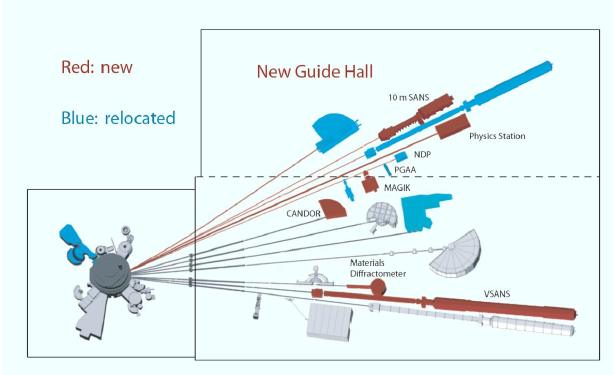
\includegraphics[width=.65\linewidth]{chapters/isotope_activation_and_radioactive_decay/images/nbsr.png}
\captionsetup{font={it}}
\caption{\acrshort{nbsr} building layout\cite{nbsrhistory}}
\label{fig:nbsrbeamlines}
\end{center}
\end{figure}




\FloatBarrier
\subsection{Spallation}

Neutrons result from fission in nuclear reactors, but spallation sources require protons and high mass targets to generate neutrons.  The energy of the protons required is a magnitude greater than that of the Scanditronix MC-40 Cyclotron at the University of Birmingham, with spallation source accelerators having a range from 500MeV to over 1GeV.  

ISIS is a neutron spallation source located in Harwell, Oxford.  Protons are accelerated in a \acrshort{linac} to 0.37c before being fed into a 163m circumference synchrotron.  The protons are then accelerated to 0.84c before being projected, in bunches, at a tungsten target.  The impact with the tungsten releases neutrons\cite{isisneutronsource}.

\acrlong{ornl} also has a neutron spallation source, the \acrshort{sns} (fig. \ref{fig:ornlspallationsource}).  A \acrshort{linac} accelerates a negatively charged proton (a hydrogen atom with two electrons) up to just below 0.9c.  It is stripped of the electrons and enters an accumulation ring as a proton.  More protons are accumulated until the beam in the accumulator is diverted at a mercury target.  The collision between the mercury target and the protons releases approximately 20 neutrons per collision, and these neutrons pass through beam lines to the experiments . 

\begin{figure}
  \begin{center}
    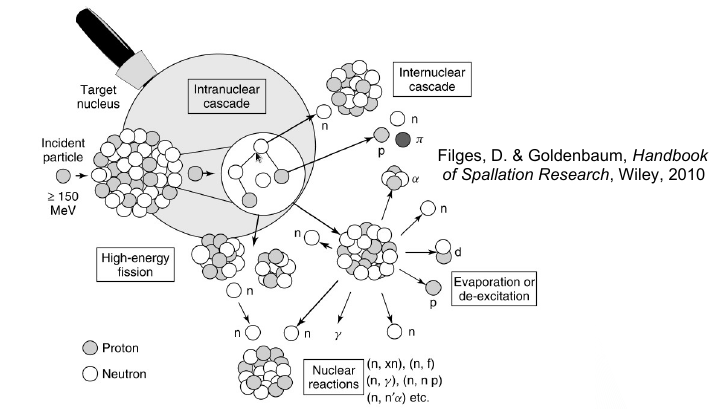
\includegraphics[width=.50\linewidth]{chapters/isotope_activation_and_radioactive_decay/images/spallation.png}
    \captionsetup{font={it}}
    \caption{An example of a neutron spallation source where high energy ions collide with heavy atoms\cite{spallationsource}}
    \label{fig:ornlspallationsource}
  \end{center}
\end{figure}

The source creates a pulse of neutrons from the 50 ton mercury target 60 times per second.  The protons are accelerated by the \acrshort{linac} to between 2.5MeV and 1.0GeV and this results in neutrons with energies almost as high as the proton projectiles.  A spectrum of neutron energies is produced with each pulse, although the neutrons may be moderated at the end of the beam lines to slow the neutrons down.




%%%%%%%%%%%%%%%%%%%%%%%%%%%%%%%%%%%%%%%%%%%%%%%%%%%%%%%%%%%%%%%%%%%%%%%%%%%%%%%%%%%%%%%%%%%%%%%%%%%%%%%%%%
%%
%%  Source Review
%%
%%%%%%%%%%%%%%%%%%%%%%%%%%%%%%%%%%%%%%%%%%%%%%%%%%%%%%%%%%%%%%%%%%%%%%%%%%%%%%%%%%%%%%%%%%%%%%%%%%%%%%%%%%


\FloatBarrier
\section{Source Review}

\begin{table}[h]
\begin{center}
\renewcommand{\arraystretch}{1.2}
\begin{tabular}{c c c c c}
\hline\hline
Source & Cost & Projectile & Flux/Current & Energy \\
\hline\hline
Scanditronix MC-40 & £1 million & Proton & $3.7 \times 10^{14}$ & 8-40MeV \\
\acrshort{hfir}\cite{hfiruserguide} &  & Neutron & $3.0 \times 10^{15}$ & Full Spectrum \\
HFIR\cite{hfiruserguide} &  & Thermal Neutron & Over $2.0 \times 10^{15}$ & Thermal \\
HFIR\cite{hfiruserguide} &  & Fast Neutron & $2.0 \times 10^{15}$ & ${}> 0.111MeV$ \\
HFIR\cite{hfiruserguide} &  & Fast Neutron & $1.0 \times 10^{15}$ & ${}> 0.821MeV$ \\
\acrshort{sns}\cite{spallationsourceflux} & \$1.4 billion & Neutron & Average $1.2 \times 10^{13}$ & Full Spectrum \\
ISIS spallation source\cite{spallationsourceflux} & & Neutron & Average $4.0 \times 10^{13}$ & Full Spectrum \\
\hline\hline
\end{tabular}
\end{center}
\caption{Examples of neutron sources, energies and flux, with the MC-40 as a reference for protons}
\end{table}

The compact proton source that is the cyclotron is compared to neutron sources.  It is much smaller and cheaper in comparison and the energy of the projectile may be controlled, whereas a spectrum of energies of neutrons is produced by reactors and spallation sources.  Faster neutrons will cause more damage to materials in \acrshort{gen4} reactors giving the cyclotron an advantage, being able to focus in just one energy range.  The three mentioned isotope sources are national facilities that cost much more than a cyclotron.  Access is shared between many researchers whereas a cyclotron, such as the Scanditronix MC-40 at the University of Birmingham may have a beam dedicated to a particular task.





%%%%%%%%%%%%%%%%%%%%%%%%%%%%%%%%%%%%%%%%%%%%%%%%%%%%%%%%%%%%%%%%%%%%%%%%%%%%%%%%%%%%%%%%%%%%%%%%%%%%%%%%%%
%%
%%  Background Activity
%%
%%%%%%%%%%%%%%%%%%%%%%%%%%%%%%%%%%%%%%%%%%%%%%%%%%%%%%%%%%%%%%%%%%%%%%%%%%%%%%%%%%%%%%%%%%%%%%%%%%%%%%%%%%



\FloatBarrier
\section[Emulating Neutron Damage]{Ion Irradiation to Investigate Neutron Damage}

Neutrons emitted during the fission of Uranium-235 have an energy spectra in the intermediate to fast range, with a peak at 1MeV, and a large proportion in the 1MeV to 10MeV range (fig. \ref{fig:u235neutronspectra}).  The higher energy neutrons are more of a concern to this work as higher energy neutrons, on colliding with atoms within the target material, cause large damage cascades.  

\begin{figure}[ht]
  \begin{center}
    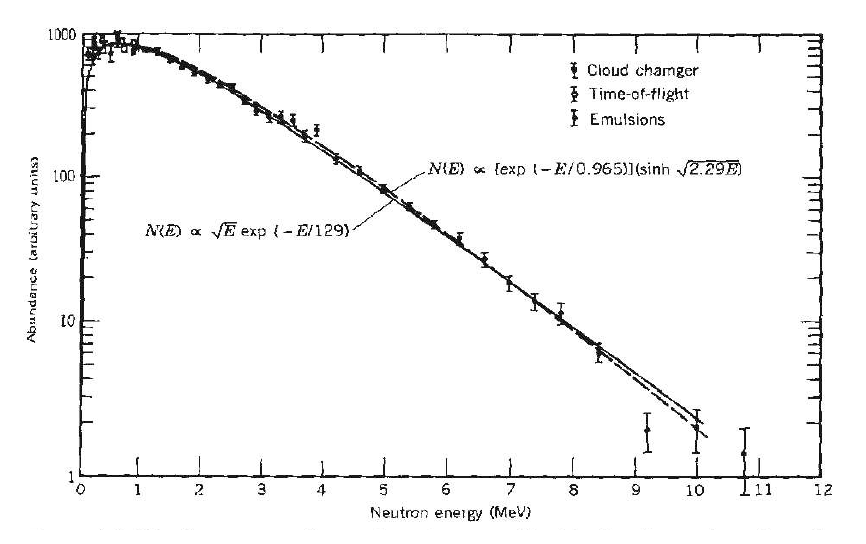
\includegraphics[width=.8\linewidth]{chapters/isotope_activation_and_radioactive_decay/plots/neutronspectrau235fission.png}
    \captionsetup{font={it}}
    \caption{Neutron Spectra from the Fission of U235\cite{leachmanneutrons}}
    \label{fig:u235neutronspectra}
  \end{center}
\end{figure}

As discussed earlier in this chapter, there are a number of methods available to create both high energy neutrons and ions, but each has its own set of advantages and disadvantages.  At the University of Birmingham high energy ions are created using a cyclotron.

\FloatBarrier

\subsection{Ion Irradiation at the University of Birmingham}

The University of Birmingham acquired a cyclotron in 2004\cite{bhamcyclotron}, the model being a Scanditronix MC-40.  It is capable of accelerating a range of light ions, to energies in the region of 10-60MeV and at currents up to 50 microamps.  In the case of protons, this is equivalent to $3.1 \times 10^{14}$ protons per second\cite{activitycpc}. 

The Cyclotron has been used to provide a steady source of radioactive isotopes for medical applications, including ${}^{18}_9 F$ for \acrfull{pept}\cite{bhamcyclotron}.  A new beam line was added for materials testing, but for this application the creation of radioactive isotopes is an unwanted by-product of the materials damage research. 

The use of neutron sources is typically expensive and the activation of atoms into radioactive isotopes is not impeded by the Coulomb barrier.  This is highlighted by cross section data for ${}^{56}_{26}Fe$ and ${}^{58}_{28}Ni$ in fig. \ref{fig:fe56ni58xs}.  The MC-40 Cyclotron is relatively inexpensive and allows materials research in a more controlled manner, given how the beam may be adjusted in terms of energy and flux as well as being focused onto a smaller area of material.


\begin{figure}[ht]
  \begin{center}
    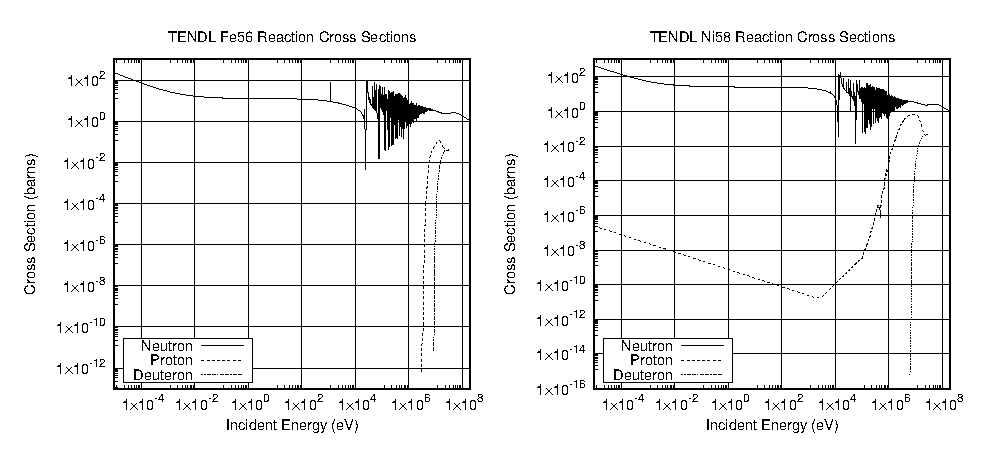
\includegraphics[width=.9\linewidth]{chapters/isotope_activation_and_radioactive_decay/plots/npd_xs/fe56_ni58_xs.eps}
    \captionsetup{font={it}}
    \caption{Neutron, proton and deuteron cross sections for Fe56 and Ni58, plotted with data from the \acrshort{tendl} database\cite{tendl2009}}
    \label{fig:fe56ni58xs}
  \end{center}
\end{figure}

In chapter \ref{chapter:activitycode} the Activity code created in this work will be discussed.  It was developed to calculate the activity of targets irradiated by the Cyclotron.  It was originally developed in Fortran\cite{activitycpc} but was rewritten in Python.  Cross section data has been generated using the TALYS code, ion transport is carried out using \acrshort{srim} and the \acrshort{jeff} \cite{jeff311} nuclear data library is used for radioactive decay data.


\FloatBarrier




\subsection{Transmutation of Nuclei by Neutrons and Protons}

\subsubsection{Neutron Activation}

The fission of Uranium-235 atoms results in neutrons with a varied spectrum of energies.  The neutrons will bounce around inside the reactor losing energy quickly to light atoms within moderators and coolants, such as water.  At lower energies the neutrons may be captured by the nuclei of atoms they interact with.  This creates a new isotope which may or may not be stable.



\subsubsection{Proton Activation}
\label{section:protonactivation}

Considering a simplified nuclear potential well, energetic protons approaching a nucleus may overcome the Coulomb potential barrier.  They are captured by the nucleus and held within the potential well by the strong nuclear force.  The barrier between a proton and a target nucleus may be approximated using eq. \ref{eq:coulombbarrier}\cite{coulombhyperphysics} and eq. \ref{eq:nuclearsize}\cite{nuclearsizehyperphysics}.  Using these equations does neglect the probability of lower energy protons being captured via quantum tunnelling of the Coulomb barrier.  These equations require the charge for the projectile ($Z_1$) and target ($Z_2$) and the nuclear radius for each ($r_1$ and $r_2$ respectively).  In order to approximate the nuclear radius using the Fermi model, the only dependency is the mass number ($A$).

\begin{equation}
V_{Coloumb} = \frac{e^2}{4 \pi \epsilon_{0}} \frac{Z_1 Z_2}{(r_{1} + r_{2})}
\label{eq:coulombbarrier}
\end{equation}

\begin{equation}
r = r_{0} A^{1/3} \text{       where } r_0 = 1.2 \times 10^{-15}m
\label{eq:nuclearsize}
\end{equation}

This process may leave the nucleus in an excited and unstable state, depending on the input energy of the proton and configuration of nucleons.  The process is probabilistic, and the average chance of a reaction (the microscopic cross section) may be measured as a function of the projectile, projectile energy and target, either experimentally or by optical model potential calculations.  

\begin{equation}
R = \frac{J}{Q} \cdot n_{\rho} \cdot \sigma \cdot 10^{-28} \delta t
\label{eq:reactioncrosssection}
\end{equation}

The reaction rate is calculated from the microscopic cross section, using eq, \ref{eq:reactioncrosssection}, and the parameters are as follows:

\begin{itemize}
\item R	Reaction Rate (reactions per second)
\item J	Beam current (A)
\item $n_{\rho}$	Number density of target (atoms per cubic metre)
\item $\sigma$ microscopic reaction cross section (barns)
\item Q projectile charge e.g $1.602177\times 10^{-19}C$ for a proton 
\item $\delta t$	target thickness (m)
\end{itemize}

The barn (unit) is the standard cross section unit for nuclear physics.  As the number density and target thickness (or track length) are given in meters, barns are converted to square meters using the factor $10^{-28}$.



\subsection{Nuclear Reaction Cross Sections}
\label{section:nuclearxs}
\subsubsection{Reaction Cross Sections}

The type of reaction for an individual event cannot be determined, but the probability of that reaction happening may be measured and future events predicted.  This data may be gathered experimentally, or it may be calculated using various models.


\FloatBarrier

\subsubsection{\Acrlong{exfor} Data File}
\label{section:exfordata}

\Acrfull{exfor} is a standard format for storing experimental results from nuclear reactions\cite{exforarticle}.  It is also associated with an online database hosted by the \acrfull{iaea} where nuclear reaction data from a variety of sources are obtained and compared. Thousands of points make up the database and the work of three groups responsible for subsets of that data was reviewed to give an insight into the methods used.

The (p,n) reactions with pure Titanium, Vanadium, Chromium, Iron and Nickel were studied by Tanaka and Furukawa\cite{exfortanaka}.  The 63 inch cyclotron that was used by the \acrfull{ins} in Tokyo provided the protons.  The device output a mono-energetic 14MeV beam of protons at a stack of target foils.  The Ti, Fe and Ni foils were $2-5 \text{mg/cm}^{2}$ in thickness, which is roughly 2-10 micrometers (depending on the density of the material).  As the ions passed through the stack of foils their energy dropped and the experimenters estimated the energy using the Bethe stopping power formula\cite{stoppingdistance}.  The ion energies in the resulting data range from 3-4MeV up to 14MeV.

Similarly the (p,n) reaction in a range of materials with 5 to 10.5MeV protons was investigated by Wing and Huizenga\cite{exforwing}.  A 60 inch cyclotron was used in this instance with foils of Vanadiuim, Chromium, Copper, Silver, Cadmium and Lanthanum.  Foils were again stacked and had a thickness of $5 \text{mg/cm}^{2}$, or approximately 5 micrometers, depending on the density of the element.  Some energies as they passed through the foils were estimated by the experimenters, based on past work.  

Vanadium, Iron and Copper foils were irradiated with 10 to 45MeV protons using the Milan \acrfull{avf} cyclotron.  In this work Gadioli et al\cite{exforgadioli} measured reaction cross sections for 17 proton energies.  Thin foils ranging from 10-48 micrometers but is it unknown whether or not they were stacked or irradiated individually using aluminium absorbers.

The experimental work as a whole ranges over decades using slightly different tools and measuring methods, but the resulting data has contributed to ever improving models used to compute the probability of a reaction.

\FloatBarrier

\subsubsection{TALYS and the Optical Model Potential}

In the standard model, protons and neutrons are composed of quarks, held together by the strong nuclear force.  The nucleus of an atom is also held together by the strong nuclear force that on such small separations overwhelms the electromagnetic force of the protons with one another.

This is a complicated system, not to mention the excited states that nuclei may occupy.  The interaction of a projectile (proton, neutron or a heavier ion) with the nucleus is a challenge to model.

Initially, reaction data for protons and neutrons were gathered through experimentation.  In the 1950s, Feshbach et al put forward a simple model for nuclear reactions between the nucleus and neutrons, and this model was restricted to 0-20MeV neutrons.  The form of the potential used was a complex function\cite{hodgson1}.

\begin{equation}
\begin{split}
V = V_0 (1 + i \zeta) r < R \\
V = 0 r > R
\end{split}
\label{eq:FeshbachPotential}
\end{equation}

The potential in equation \ref{eq:FeshbachPotential} has the parameters $R = 1.45 \times A^{\frac{1}{3}}$, $V_0 = 42MeV$ and $\zeta = 0.03$ where A is the atomic mass of the target atom.  These parameters were fit to the experimental data available to Feshbach et al\cite{feshbach} with the only variable being the atomic mass\cite{hodgson1}.

Considering the complexity of the system being modelled, this simple model was very successful.  Over the years since, the models used have become more complex and parameters used have been fit to an increasing amount of experimental data.

The TALYS code uses a range of models (fig. \ref{fig:talysworkflow}).  These include the optical model which is solved using the \acrlong{ecis} (ECIS-06) code of Jacques Raynal, implemented as a subroutine within TALYS, and this is accurate up to 180MeV\cite{talysmanual}.  Whilst the TALYS code has been extended up to 1GeV, it is experimental in the 180MeV to 1GeV range.  Fortunately, this work only requires nuclear reaction cross section data up to approximately 100MeV as the current ion source under consideration produced ions with energies up to 60MeV.

\begin{figure}[tbp]
  \begin{center}
    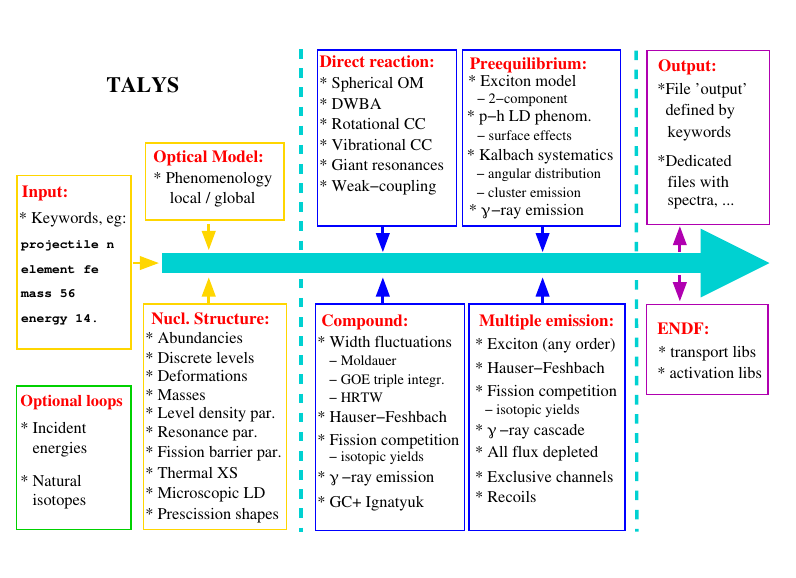
\includegraphics[width=.6\linewidth]{chapters/isotope_activation_and_radioactive_decay/images/talys.png}
    \captionsetup{font={it}}
    \caption{TALYS work flow \cite{talysmanual}}
    \label{fig:talysworkflow}
  \end{center}
\end{figure}

The TALYS code has potentials for protons and neutrons, but it also has potentials for deuterons, tritons, helium-3 and alpha particles.  The potentials are discussed in detail in the TALYS manual\cite{talysmanual}.  This extension to heavier ions may be useful for this work as the University of Birmingham cyclotron is capable of accelerating deuterons and $He^{2+}$ ions.

\begin{figure}[h]
  \begin{center}
    \includegraphics[width=.75\linewidth]{chapters/isotope_activation_and_radioactive_decay/images/Fe54-Co55.png}
    \captionsetup{font={it}}
    \caption{TALYS Fe54-Co55 cross section comparison with experiment \cite{tendlfeco}}
    \label{fig:Fe54-Co55}
  \end{center}
\end{figure}

Comparing experimental data to the TALYS data for $Fe54(p, \gamma)Co55$ shows good agreement between 1MeV and 10MeV.  There was insufficient experimental data from this source, but the TALYS generated data ranges from micro eV up to 100MeV+, as seen in fig. \ref{fig:Fe54-Co55}\cite{tendlfeco}.


\FloatBarrier
\subsubsection{Proton Activation Data File}

The \acrfull{padf} was released in 2007 and contained nuclear reaction data for 2355 target nuclei, ranging from Magnesium (12) to Radon (86) with proton energies up to 150MeV.  The file contains the sum of all individual reactions as well as certain yields, and the data was generated using the TALYS and ALICE/ASH codes, as well as experimental data from Exfor\cite{exforlink}.

\begin{lstlisting}[style=sFortran,caption={A sample of the Iron-56 PADF data file}]
             Proton Activation Data File                           528 1451   12
             ***************************                           528 1451   13
                                                                   528 1451   14
  Authors: C.H.M.Broeders, U.Fischer, A.Yu.Konobeyev, L.Mercatali  528 1451   15
                                                                   528 1451   16
                                                                   528 1451   17
  Data for PADF file were obtained using the TALYS code [1] for    528 1451   18
  target nuclei with half-life more than 10 min and using the      528 1451   19
  ALICE/ASH code [2] for nuclei with 1 sec < T1/2 < 10 min and     528 1451   20
  available experimental data                                      528 1451   21
     MAT numbers are taken according to JEFF-3.1/RDD               528 1451   22
                                                                   528 1451   23
  Evaluation for Fe-56 (stable) :  TALYS code                      528 1451   24
  Experimental data used for the correction of calculated          528 1451   25
  excitation functions are taken from Refs.[3-12]                  528 1451   26
                                                                   528 1451   27
                                                                   528 1451   28
  File contains                                                    528 1451   29
                                                                   528 1451   30
  MF=3  MT=5                                                       528 1451   31
        Sum of all individual reaction cross-sections (Total       528 1451   32
        reaction cross-section)                                    528 1451   33
                                                                   528 1451   34
  MF=6  MT=5                                                       528 1451   35
        Yields of nuclei in nuclear reactions including            528 1451   36
        n, p, d, t, He-3, He-4 and photon production               528 1451   37
\end{lstlisting}



\subsubsection{TENDL 2019 Data Files}

The cross section data for protons and neutrons is available to download in \acrshort{endf} format files.  The data sources used by this work are the TALYS code and \acrshort{tendl} data files, and these are created by a combination of different nuclear models and experimental data.  The \acrshort{tendl} nuclear reaction simulation code provides the calculated data.

The nuclear reaction files are rather large, and they all follow a standard format.


\begin{lstlisting}[style=sPseudo,caption={Sample TENDL File}]
 2.605600+4 5.545443+1          0          0          0          02631 3  2    1
 0.000000+0 0.000000+0          0          0          1         462631 3  2    2
         46          2                                            2631 3  2    3
 1.000000+3-9.920042-7 1.000000+6-9.920042-7 2.000000+6-2.167241-42631 3  2    4
 3.000000+6-7.609736-3 4.000000+6-3.232345-2 5.000000+6-5.975554-22631 3  2    5
 6.000000+6-5.149510-2 7.000000+6-3.685484-2 8.000000+6-5.542173-22631 3  2    6
 9.000000+6-9.978765-2 1.000000+7-1.599116-1 1.100000+7-2.206871-12631 3  2    7
 1.200000+7-2.743084-1 1.300000+7-3.165007-1 1.400000+7-3.471231-12631 3  2    8
 1.500000+7-3.674350-1 1.600000+7-3.788282-1 1.700000+7-3.825634-12631 3  2    9
 1.800000+7-3.799978-1 1.900000+7-3.725944-1 2.000000+7-3.617662-12631 3  2   10
 2.200000+7-3.342054-1 2.400000+7-3.031296-1 2.600000+7-2.709398-12631 3  2   11
 2.800000+7-2.388019-1 3.000000+7-2.077513-1 3.500000+7-1.398614-12631 3  2   12
 4.000000+7-8.801994-2 4.500000+7-5.013441-2 5.000000+7-2.349373-22631 3  2   13
 5.500000+7-5.480233-3 6.000000+7 6.189980-3 6.500000+7 1.332313-22631 3  2   14
 7.000000+7 1.727774-2 7.500000+7 1.906833-2 8.000000+7 1.943711-22631 3  2   15
 9.000000+7 1.783081-2 1.000000+8 1.499871-2 1.100000+8 1.211197-22631 3  2   16
 1.200000+8 9.641120-3 1.300000+8 7.717424-3 1.400000+8 6.318436-32631 3  2   17
 1.500000+8 5.367555-3 1.600000+8 4.771939-3 1.800000+8 4.312985-32631 3  2   18
 2.000000+8 4.445323-3                                            2631 3  2   19
\end{lstlisting}








\subsection{Radioactive Decay}

Radioactive decay is the random change in nucleons or energy state of an unstable nucleus.  It is impossible to predict when a single nucleus will decay, but the decay of a collection of nuclei is statistical in nature.  The radioactivity and number of unstable nuclei at time (t) can be predicted using the decay constant (\textlambda) for the radioactive isotope.  This constant is defined as follows:

\begin{equation}
\lambda = - \frac{N'(t)}{N(t)}
\end{equation}

The number of radioactive nuclei $N(t)$ at time t is given by the following equation, where $N(0)$ is the starting number of nuclei:

\begin{equation}
N(t) = N(0) \exp(-t \lambda)
\end{equation}

The activity $A(t)$ of the radioactive nuclei is predicted at time t by using the following equations, where $N'(t)$ is the change in amount of nuclei with respect to time:

\begin{equation}
A(t) = -N'(t) = \lambda N(t)
\label{eq:activityofanisotope}
\end{equation}
\begin{equation}
A(t) = \lambda N(0) \exp(-t \lambda)
\end{equation}

\subsection{Saturation Activity}

As a radioactive isotope is created by reactions between target atoms and projectiles (protons, neutrons, deuterons) it will begin to decay.  The amount of the isotope will continue to increase until the decay rate equals the reaction rate for the creation of the isotope.

For a single isotope the production rate ($\omega$) is calculated using the ion current ($J$), the charge per ion ($Q$), the number density of atoms in the target ($n_{\rho}$), the reaction cross section ($\sigma$) and the track length ($\delta t$), as given in eq. \ref{eq:reactionrate}.  The units are amps and coulombs for the current and charge, whereas the cross section is in barns and the number density in atoms per cubic meter.  The track distance is measured in meters.  This necessitates the conversion from barns to square meters, hence the factor $10^{-28}$.

\begin{equation}
\begin{split}
\omega = \frac{J}{Q} \cdot n_{\rho} \cdot \sigma \cdot 10^{-28} \delta t
\end{split}
\label{eq:reactionrate}
\end{equation}

The change in the amount of an isotope with time ($\frac{dN}{dt}$) is the source rate minus the loss rate ($\lambda N$) as given in eq. \ref{eq:isotopechange}.  This is given as the initial condition the starting amount $N_0$ at time $t = 0$.

\begin{equation}
\begin{split}
\frac{dN}{dt} = \omega - \lambda N, N(0) = N_0
\end{split}
\label{eq:isotopechange}
\end{equation}

This equation may be solved using Laplace transforms (appendix \ref{chapter:usefullaplacetransforms}) and this will be explored in more detail in section \ref{section:laplaceequations}.  The solution for a single isotope that has a starting amount $N_0$, a decay constant $\lambda$ and a creation rate of $\omega$ is given in eq. \ref{eq:decayequationoneisotope}.

\begin{equation}
\begin{split}
N(t) = \frac{\omega}{\lambda} + \left(N_{0} - \frac{\omega}{\lambda} \right) \exp(-\lambda t)
\end{split}
\label{eq:decayequationoneisotope}
\end{equation}

The saturation activity may be computed as follows.  As t approaches infinity the exponential term tends towards zero due to the negative decay constant.  Replacing the exponential terms with zero and noting eq. \ref{eq:activityofanisotope} leaves a simple result to compute the saturation activity ($A_{s}$) (eq. \ref{eq:saturationactivity}).  This is logical as, once saturated, the isotope will decay at the same rate as its source.

\begin{equation}
\begin{split}
N_{s} = \frac{\omega}{\lambda} \\
A_{s} = \lambda N_{s} = \omega \\
\end{split}
\label{eq:saturationactivity}
\end{equation}

The saturation time lies on an asymptote, therefore the saturation time is undefined.  Rather than attempt to compute this time it is more useful to compute the time at which the saturation reaches a fraction (k) of the maximum saturation amount ($N_{s}$).

\begin{equation}
\begin{split}
k N_{s} = \frac{\omega}{\lambda} + \left(N_{0} - \frac{\omega}{\lambda} \right) \exp(-\lambda t) \\
t = \frac{-1}{\lambda} \ln \left[ \frac{k-1}{N_0 \frac{\lambda}{\omega} - 1} \right] \\
\end{split}
\label{eq:saturationactivity}
\end{equation}

The equation is useful in calculating (near to) the maximum possible activity of a isotope being created in a proton beam or other similar process where radioactive isotopes are created and lost at a constant rate.


\subsection{Decay Constants: \acrfull{jeff} 3.3 Data File}

\acrshort{jeff} 3.3 is an evaluated data file\cite{jeff311}, meaning it has been evaluated by a relevant authority.  The quality of the data may affect the health of the public and industry workers, so it must be evaluated.  This particular file is managed by and available through the \acrfull{nea}.

It is a collection of many data files.  Released in 2017, it also contains several files for incident gammas, protons, deuterons, tritons, helium-3 and alphas from the \acrshort{tendl} 2017 data file.

The files that will be important for this work are the \acrshort{endf}-6 radioactive decay data files only.  The nuclear reaction cross section data will come from TALYS and various iterations of the \acrshort{tendl} libraries.  The decay data held in the \acrshort{jeff} 3.3 file includes isotope data, masses, half lives, branching factors, continuous and discrete gamma data.


\subsection{Bateman Equation for Radioactive Decay}

%% Define tikz boxes
\tikzstyle{startstop} = [rectangle, rounded corners, minimum width=3cm, minimum height=1cm,text centered, draw=black, fill=grey!30]
\tikzstyle{process} = [rectangle, minimum width=3cm, minimum height=1cm, text centered, draw=black, fill=grey!10]
\tikzstyle{arrow} = [thick,->]

\begin{figure}[!h]
\centering
\begin{tikzpicture}[node distance=2cm]
\node (parent) [startstop] {Parent Isotope, N$_{\text{1}}$(t)};
\node (isotope1) [process, below of=parent] {1st Unstable Daughter Isotope, N$_{\text{2}}$(t)};
\node (isotope2) [process, below of=isotope1] {2nd Unstable Daughter Isotope, N$_{\text{3}}$(t)};
\node (stable) [startstop, below of=isotope2] {Stable Daughter Isotope, N$_{\text{4}}$(t)};
%% arrows
\draw [->] (parent) -- (isotope1);
\draw [->] (isotope1) -- (isotope2);
\draw [->] (isotope2) -- (stable);
\end{tikzpicture}
\captionsetup{font={it}}
\caption{An example decay chain from an unstable parent isotope, through unstable daughter isotopes ending with a stable daughter isotope.}
\label{fig:decaychain}
\end{figure}

The English mathematician Harry Bateman derived an equation (eq. \ref{eq:bateman}\cite{bateman}\cite{batemanequation}) to calculate the amount of each isotope in a decay chain, illustrated in fig. \ref{fig:decaychain}, at time t.  $N$ is the isotope amount and $n$ denotes the nth isotope in that decay chain.  The decay constant ($\lambda$) is required for each isotope in the decay chain along with the starting amount for the first isotope in the decay chain ($N_1(0)$).

\begin{equation}
N_{n}(t) = \frac{N_1(0)}{\lambda_n} \sum_{i=1}^{n} \left[ \prod_{j=1, i\ne j}^{n} \frac{\lambda_j}{\lambda_j - \lambda_i}\right] \exp(-\lambda_i t) 
\label{eq:bateman}
\end{equation}

This equation (eq. \ref{eq:bateman}) allows the user to calculate how much of each isotope there is expected to be at some time in the future, where each of the isotopes in the decay chain is decaying.

When a radioactive isotope decays, there may be more than one mode of decay, and this leads to branching factors.  Pb-214 only decays via beta decay to Bi-214, giving a branching factor of 1.0, whereas Bi-214 has a 99.979\% chance of decaying to Po-214 by beta decay and a 0.021\% of emitting an alpha particle and decaying to Tl-210 (branching factors of 0.99979 and 0.00021 respectively) \cite{jeff311}.

When a target material is irradiated, there is a source term for transmuted nuclei due to the irradiation.  The daughter isotopes of these transmuted isotopes will also be affected by the irradiation and will transmute further, giving a source term for each daughter isotope as a result of the irradiation.  Sources for each isotope in the decay chain, and branching factors between a parent isotope and its daughter isotope/s must be accounted for.  This is addressed in chapter \ref{chapter:activitycode}.





\section[Using SRIM and TRIM]{Simulating Ion Irradiation with SRIM and TRIM}
\label{section:srimtrim}

A package of ion transport codes, \acrshort{srim}, is freely available to download and use to investigate the transport of ions through matter.  It includes tools to calculate the stopping range of a given ion in a material as well as \acrlong{trim}, a code used to calculate the energy and position of an ion through a target.

\acrshort{trim} does not take into account the structure of a target.  It may be layered in the calculation perpendicular to the beam, but beyond that the target is treated as amorphous.  It will give the same result for BCC iron as it would for FCC iron, providing the density remains the same.  The density and whether or not the target layer is a gas or solid are options that must be configured when setting up a calculation.  Each ion history is tracked through the same target; the target never changes.  \acrshort{trim} is ignorant to the structure and therefore damage to the structure that would accumulate over time, and to any swelling and change in composition or density.

The interaction of the ion with the target material is split into two parts: nuclear loss and electronic loss.  The ion is tracked through the target until either its energy drops below a set threshold (10eV) or it leaves the target (fig \ref{fig:fe13traj}).  The code then moves on to the next ion history.

In a projectile-nucleon interaction a number of equations were developed by Biersack et al\cite{srimbook} where a number of parameters are fit for the screened potential.  They are used to determine the scattering angle $\Theta$ of the ion and target nucleus, as well as the amount of energy transferred.  The azimuthal angle is selected randomly by multiplying $2\pi$ by a random float $[0.0, 1.0]$.

The screening length ($a$) is dependent upon the charge of the projectile ($Z_1$) and that of the target ($Z_2$) (eq. \ref{eq:screeninglength}).

\begin{equation}
\begin{split}
a = \frac{0.8853 a_0}{\left(Z_1^{\frac{2}{3}} + Z_2^{\frac{2}{3}}\right)}
\end{split}
\label{eq:screeninglength}
\end{equation}

\begin{equation}
\begin{split}
\epsilon \equiv \frac{a E_c}{Z_1 Z_2 e^{2}}
\end{split}
\label{eq:reducedenergy}
\end{equation}

The scattering angle ($\Theta$) is computed using eq. \ref{eq:magicformula1}.  It is dependent upon the screening length (eq. \ref{eq:screeninglength}) as well as the reduced energy ($\epsilon$) (eq. \ref{eq:reducedenergy}).  Five other parameters were fit ($C_1$ to $C_5$) by Biersack and these are given in eq. \ref{eq:magicformula2}.

\begin{equation}
\begin{split}
cos \left(\frac{\Theta}{2}\right) = \frac{B + R_c + \Delta}{R_0 + R_C} \\
\text{where } \\
B = \frac{p}{a} \text{,    }  R_0 = \frac{r_0}{a} \text{,    }  R_C = \frac{\rho}{a} \\
\Delta = A \frac{R_0 - B}{1 + G} \\
\end{split}
\label{eq:magicformula1}
\end{equation}

\begin{equation}
\begin{split}
A = 2 \alpha \epsilon B^\beta \\
G = \gamma \left(\left(1+A^2\right)^{\frac{1}{2}}-A\right)^{-1} \\
\alpha = 1 + C_1 \epsilon^{-\frac{1}{2}} \text{,    } \beta = \frac{C_2 + \epsilon^{\frac{1}{2}}}{C_3 + \epsilon^{\frac{1}{2}}} \text{,    } \gamma = \frac{C_4 + \epsilon^{\frac{1}{2}}}{C_5 + \epsilon^{\frac{1}{2}}} \\
\text{where } p \text{ is the impact parameter} \\
\text{where } a \text{ is the screening length} \\
\text{where } r_0 \text{ is the distance of closest approach} \\
\text{where } \epsilon \text{ is the reduced energy} 
\end{split}
\label{eq:magicformula2}
\end{equation}

The potential between the projectile and target is calculated at the distance of closest approach, $r_0$.  It is a Coulomb type potential (eq. \ref{eq:interatomicpotential}) than includes the universal screening function (eq. \ref{eq:universalscreening})\cite{srimbook}.  This potential will appear again, although occasionally with differing parameters, in chapter \ref{chap:backgroundfitting}.  The parameters defined here in eq. \ref{eq:universalscreening} are those derived and published by Ziegler, Ziegler and Biersack in the 2015 \acrshort{srim} book\cite{srimbook}.

\begin{equation}
V(R) = \frac{Z_1 Z_2 e^2}{a R} \Phi(R)
\label{eq:interatomicpotential}
\end{equation}

\begin{equation}
\Phi(R) = 0.1818 \exp(-3.2 x) + 0.5099 \exp(-0.9423 x) + 0.2802 \exp(-0.4028 x) + 0.2817 \exp(-0.2016 x)
\label{eq:universalscreening}
\end{equation}

The recoil nuclei are also followed through several generations until their energies fall below that set for either the surface binding energy or displacement energy (3-6eV and 15-30eV respectively)\cite{srimbook}.  

The free flight path between large collisions is calculated based on the projectile energy, type and the target material.  The path length between collisions is randomly generated by taking the maximum free path and multiplying by a random float $[0.0, 1.0]$.  Smaller projectile-nucleus interactions are not individually calculated, but the average energy that would have been lost is calculated and applied.

The ion continuously loses energy to the electrons in the material.  \acrshort{trim} calculates this over the free flight path, L (eq. \ref{eq:electronicstopping}).

\begin{equation}
\begin{split}
\Delta E_e = L N S_e (E) \\
\text{where } S_e (E) \text{ is the electronic stopping} \\
\text{and } N \text{ is the atomic density of the target} \\
\end{split}
\label{eq:electronicstopping}
\end{equation}

The target damage is a combination of the incoming ion, the primary knock on atoms and their damage cascades.  The user has the option of running a full damage cascade that plots the entire cascade, or a quicker calculation where the cascade is treated as just a point.  The total number of displacements is the sum of vacancies and replacement collisions, and the vacancies is sum of interstitials with the number of atoms that leave the target.

\begin{figure}
  \begin{center}
    \includegraphics[width=.7\linewidth]{chapters/isotope_activation_and_radioactive_decay/plots/fe_13MeV.eps}
    \captionsetup{font={it}}
    \caption{One hundred simulated 13MeV proton energy loss curves in Fe simulated with SRIM \cite{srim}}
    \label{fig:fe13traj}
  \end{center}
\end{figure}

One file that \acrshort{srim} creates is of importance to the Activity code, and that is the trajectory file that contains the energy and x,y,z co-ordinate data points for simulated ions moving through matter.  Fig. \ref{fig:fe13traj} shows the trajectory of one hundred 13MeV protons entering and passing through an Iron target, and it is this set of data points (together with the cross section database) that the Activity code uses to calculate the reaction rates for the transmutation of nuclei in the target.  At higher energies, the ions slow as they lose energy due to electronic stopping, but as the ion energy drops the mechanism of loss through nuclear collisions becomes important.  The spreading of ion depths at lower energies is a result of the higher momentum transfer during nuclear collisions.










\chapter[Interatomic Potential Fitting]{Interatomic Potential Fitting}
\label{chap:backgroundfitting}

\begin{changemargin}{1.0cm}{1.0cm}
\abstractpreamble{In order to model \Gls{Fe}, \Gls{Pd} and \Gls{Ru} with Molecular Dynamics codes, an interatomic potential is needed.  This will require experimental data and data generated by first principles calculations.  The simplified models will consist of just Fe-Pd and Fe-Ru, but pure Fe does not take the \acrshort{fcc} structure that it does when alloyed with \Gls{Ni} in Austenitic Stainless Steel.  \\
\\
The properties of theoretical pure \acrshort{fcc} Fe are estimated using Density Functional Theory that solves the many body Schr\"{o}dinger Equation.  While it is impossible to solve this equation exactly, with our current technology and knowledge, it is possible to solve approximately by making several approximations and by using the Hohenberg-Kohn theorem.\\
\\
Many body potentials such as the \acrshort{fs} and \acrlong{eam}  are often used to model metals.  The force matching method is used to fit the potentials to data.  Optimization algorithms are split into global and local, with an example of a global being simulated annealing and a local being \acrshort{bfgs}.}
\end{changemargin}





%%%%%%%%%%%%%%%%%%%%%%%%%%%%%%%%%%%%%%%%%%%%%%%%%%%%%%%%%%%%%%%%%%%%%%%%%%%%%%%%%%%%%%%%%%%%%%%%%%%%%%%%%%
%%
%%  Experiment, Modelling and Theory
%%
%%%%%%%%%%%%%%%%%%%%%%%%%%%%%%%%%%%%%%%%%%%%%%%%%%%%%%%%%%%%%%%%%%%%%%%%%%%%%%%%%%%%%%%%%%%%%%%%%%%%%%%%%%


\FloatBarrier
\section{Experiment, Modelling and Theory}

\subsection{Introduction}

We do not have a complete understanding of the world around us, so it may be that experiment is the \enquote{best} method of testing a material, as by its nature it will obey the rules of physics.  As far as we know, these do not change from one place to another.  A piece of steel used in an experiment is never going to have precisely the same composition and structure as similar steel use in a reactor, but it should be close enough.

The \acrlong{sem} has a magnification of approximately 1 million times and they are able to generate a picture of the surface of a specimen using a beam of electrons.  The \acrlong{tem} has the ability to magnify a specimen further, with a resolution of less than 1 angstrom.  The trade off is that a it covers a smaller area of the specimen than a \acrshort{sem} and the sample must be prepared in thin slices.

The composition of an irradiated sample may be tested by a number of methods including \acrlong{naa} and \acrlong{sims}.  Scattering techniques, such as x-ray or neutron diffraction, can give an insight into the structure of a material, but they are statistical methods and do not give detailed measurements of individual atoms or defects.

There are draw backs to experiments, several of which are particular to this work.  Even with our advances in technology, there are still errors introduced into any experiment.  When dealing with smaller and smaller volumes of atoms quantum effects will also need to be considered.

Radiation damage experiments, whether by neutrons or ions, will result in radioactive waste and the target must be safe to handle to be examined.  The collision event happens up to a micron or more into the material.  They occur on a very short timescale and within small volumes of space at random points along the path of the projectile, so the events would be very hard or impossible to track as they occur with current technology.

Current theories have been developed and modified over hundreds of years, and in the last 100 years Quantum Mechanics has been introduced to better describe physics on a small scale.  It is a well proven theory that has been very successful.  Unfortunately, using the theory exactly for a large ensemble of atoms and electrons is impossible with our current level of technology.

Computer models use theory, and a number of approximations, to simulated reality.  These models may need to be fine tuned, to better fit both the theory and experiment, but they allow us to do what is not possible with either experiment or theory.  It is possible to simulate an individual damage cascade and watch it in fine detail spatially and temporally.  As computer power increases, the models used become more complex and the simulation boxes and time spans grow.

This chapter discusses the background required to link the more accurate \acrshort{dft} to \acrshort{md} by deriving  interatomic potentials based on experiment and calculated data.  By doing this, it opens a route to model the concentrations of \acrshort{pgm}s at the grain boundary following irradiation damage.



\FloatBarrier
\subsection{Simulating Materials on a Variety of Scales in Time and Space}

Taking a 1 micron grain in a steel as an example, it would contain tens of billions of atoms.  This is too large a number of atoms to model currently, but by choosing the right type of model a portion of the grain may be modelled.


\begin{figure}[htbp]
  \begin{center}
    \includegraphics[width=10.0cm]{chapters/interatomic_potential_fitting/images/scale.png}
    \captionsetup{font={it}}
    \caption{Time and Size Scales for Computer Packages \cite{scalediagram}}
    \label{fig:timesizascalesmodelling}
  \end{center}
\end{figure}

The properties of metals may be approximated using small crystals rather than the whole grain, and this is ideally suited to \acrshort{dft} calculations.  Simulations of small ensembles of atoms over time are now also possible using \acrshort{dft} molecular dynamics.  Larger simulations containing thousands to millions of atoms, that are able to simulate single damage cascades are suitable for \acrshort{md} simulations (figure \ref{fig:timesizascalesmodelling}). 




%%%%%%%%%%%%%%%%%%%%%%%%%%%%%%%%%%%%%%%%%%%%%%%%%%%%%%%%%%%%%%%%%%%%%%%%%%%%%%%%%%%%%%%%%%%%%%%%%%%%%%%%%%
%%
%%  Properties of Crystals
%%
%%%%%%%%%%%%%%%%%%%%%%%%%%%%%%%%%%%%%%%%%%%%%%%%%%%%%%%%%%%%%%%%%%%%%%%%%%%%%%%%%%%%%%%%%%%%%%%%%%%%%%%%%%

\section{Properties of Crystals}

\subsection{Introduction}

There are seven crystal classes (table. \ref{table:crystalclasses}) and 14 Bravias lattices (section \ref{section:crystalsrecipbloch}), although this work is primarily concerned with cubic and \gls{orthorhombic} crystals.    

\begin{table}[h]
\begin{center}
\renewcommand{\arraystretch}{1.2}
\begin{tabular}{c c c}
\hline\hline
Class & Lengths & Angles \\
\hline\hline
Cubic & $a = b = c$ & $ \alpha = \beta = \gamma = 90^{\circ}$ \\
Hexagonal & $a = b, c $ & $ \alpha = \beta, \gamma = 120^{\circ}$ \\
Rhombohedral & $a = b = c $ & $ \alpha = \beta = \gamma \neq 90^{\circ}$ \\
Tetragonal & $a = b, c $ & $ \alpha = \beta = \gamma = 90^{\circ}$ \\
Orthorhombic & $a, b, c $ & $ \alpha = \beta = \gamma = 90^{\circ}$ \\
Monoclinic & $a, b, c $ & $ \alpha = \beta = 90^{\circ}, \gamma \neq 90^{\circ} $ \\
Triclinic & $a, b, c $ & $ \alpha, \beta, \gamma, $ \\
\hline\hline
\end{tabular}
\caption{Seven Crystal Classes}
\label{table:crystalclasses}
\end{center}
\end{table}

Metals are rarely single crystals, but are made from many crystals separated by grain boundaries.  However, the knowledge of the microscopic crystals translates well to the properties of the metals on a macroscopic scale.

This work does not attempt to calculate properties based on a collection of many crystals, but on a single crystal with less that a thousand atoms.  The crystals are then assumed to be infinite in size, due to periodic boundary conditions.



\subsection{Equation of State}

The equation of state of a material relates either the pressure on that material as a function of the volume, or the energy of a sample of a material to the volume.  This not only allows one to predict the energy or pressure at a certain volume, but also the minimum energy, relaxed volume and the bulk modulus.

\subsubsection{Bulk Modulus}

The bulk modulus of a material is defined as the bulk stress of a sample divided by the bulk strain on that sample and several example values are given in table \ref{table:examplebulkmodulii}.  It is also the inverse of the compressibility of that material, which means that materials with a higher bulk modulus are less compressible than those with a lower value.

\eqBulkModulusA

\eqBulkModulusB

\begin{table}[h]
\begin{center}
\renewcommand{\arraystretch}{1.2}
\begin{tabular}{c c}
\hline\hline
Material & Bulk Modulus/GPa \\
\hline\hline
Aluminium & 70 \\
Iron (BCC) & 110 \\
Stainless Steel 18-8 & 163 \\
\hline\hline
\end{tabular}
\end{center}
\caption{Example bulk modulii for three metals}
\label{table:examplebulkmodulii}
\end{table}

\subsubsection{Murnaghan Equation of State}

Hooke's law implies a linear relationship between stress and strain.  In practice, where a pressure is applied to a material, the application of Hooke's law is limited\cite{murnaghaneq}.  Muraghan derived a new equation to improve upon formulae developed in the 1930's, using compression data from high pressure experiments.

\begin{equation}
\begin{split}
P(V) = \frac{B_0}{{B'}_0}\left(\left(\frac{V_0}{V}\right)^{{B'}_0}-1\right)
\end{split}
\label{eq:eqMurnachanEquationofStatePressure}
\end{equation}

As pressure is the negative derivative of the internal energy of the system with respect to change in volume, $p = -(\partial E/dV)$, and the equation can be integrated and written in terms of the energy, volume, bulk modulus and its derivative\cite{crystaleos}.

\begin{equation}
\begin{split}
E(V) = E_0 + \frac{B_0 V}{{B'}_0} \left[\left(\frac{V_0}{V}\right)^{{B'}_0} \frac{1}{{B'}_0 - 1} + 1 \right] - \frac{B_0 V_0}{{B'}_0-1}
\end{split}
\label{eq:eqMurnachanEquationofStateEnergy}
\end{equation}

\subsubsection{Birch-Murnaghan Equation of State}

Several years after Murnaghan's equation, Birch developed the equation of state further upon the experimental data provided by work from Bridgman in high pressure physics.  For cubic symmetry, the description of free energy now includes third order terms in the strain components\cite{birchmurnaghaneq}.

\begin{equation}
\begin{split}
P(V) = \frac{3 B_0}{2} \left[\left(\frac{V_0}{V}\right)^{\frac{7}{3}}-\left(\frac{V_0}{V}\right)^{\frac{5}{3}}\right] \left[1 + \frac{3}{4}({B'}_0-4)\left(\left(\frac{V_0}{V}\right)^{\frac{2}{3}}-1\right)\right]
\end{split}
\label{eq:eqMurnachan Equation of State}
\end{equation}

The energy-volume relationship may again be constructed\cite{crystaleos}.

\begin{equation}
\begin{split}
E(V) = E_0 + \frac{9 V_0 B_0}{16} \left[ \left[ \left(\frac{V_0}{V} \right)^{\frac{2}{3}}-1\right]^{3} {B'}_0 + \left[ \left(\frac{V_0}{V} \right)^{\frac{2}{3}}-1\right]^{2} \left[6 - 4 \left(\frac{V_0}{V} \right)^{\frac{2}{3}}\right] \right]
\end{split}
\label{eq:eqMurnachanEquationofStateVolume}
\end{equation}

In order to fit the Birch-Murnaghan, the first step is to fit a second order polynomial to the energy-volume data.  This may be achieved using least-squares fitting with a vandermode matrix.  The coefficients from this polynomial may then be used to calculate reasonable values for $E_0$, $V_0$ and $B_0$; sane starting values of ${B'}_0$ are between 1 and 10, and a recommended value in the literature is 2\cite{gilgamesheos}.

\begin{equation}
\begin{split}
E(V) = c_0 + c_1 V + c_2 V^2 \\
V_0 = -\frac{c_1}{2c_2} \\
E_0 = c_2 \times {V_0}^2 + c_1 V_0 + c_0  \\
B_0 = 2 c_2 V_0 \\
{B'}_0 = 2
\end{split}
\label{eq:eqMurnachanEquationofStateVolume}
\end{equation}

Newton Gauss (eq. \ref{eq:eqNGBMfit}) may then be used to attempt to minimise the fit further for $E_0$, $V_0$ and $B_0$ whilst trying values of ${B'}_0 \in {1.0,1.5,2.0,2.5,3.0,3.5,4.0,4.5,5.0,5.5,6.0}$.  The parameters with the lowest residual square sum are returned.

\begin{equation}
\begin{split}
\left[J^T J\right] P = J^T R
\end{split}
\label{eq:eqNGBMfit}
\end{equation}

Mehl et al used a version of the Birch equation of state\cite{birchmurnaghaneq} and suggest a value for ${B'}_0$ between 3 and 5\cite{mehlsp} and limit the value of N in eq. \ref{eq:eqBirchMehlEtAl} to either 3 or 4 for the best data fit.

\begin{equation}
\begin{split}
E(V) = E_0 + \frac{9}{8} B_0 V_0 \left[ \left(\frac{V_0}{V}\right)^{\frac{2}{3}} - 1 \right]^{2} + \frac{9}{16} B_0(B_0^{'} - 4) V_0 \times \left[ \left(\frac{V_0}{V}\right)^{\frac{2}{3}} - 1 \right]^{3} + sum_{n=4}^{N} \gamma_n \left[ \left(\frac{V_0}{V}\right)^{\frac{2}{3}} - 1 \right]^{n}
\end{split}
\label{eq:eqBirchMehlEtAl}
\end{equation}

In generating the data for a Birch or Birch-Murnaghan fit the atom configuration is relaxed.  A small strain $\left[\sigma, \sigma, \sigma, 0.0, 0.0, 0.0\right]$ is applied to decrease and increase the volume slightly about the relaxed volume.


\FloatBarrier
\subsubsection{Rose-Vinet Equation of State}
\label{section:rosevineteos}

\begin{equation}
\begin{split}
E(a) = E_0 + \left(1 + -\alpha \left(\frac{a}{a_0 - 1}\right)\right) exp\left(-\alpha \left(\frac{a}{a_0 - 1}\right)\right) 
\alpha = \sqrt{\frac{9 \Omega B_0}{-E0}}
\end{split}
\label{eq:eqRoseVinet}
\end{equation}

More recently a Universal form, eq \ref{eq:eqRoseVinet}, was proposed by Rose, Vinet et al\cite{rosevinet}.  With an exponential cut off, this fits from the relaxed lattice parameter to much wider separations with a good fit for simple and transition metals, including K, Mo, Cu (fig. \ref{fig:rosevinet}).

\begin{figure}[htbp]
  \begin{center}
    \includegraphics[width=.5\linewidth]{chapters/interatomic_potential_fitting/images/rosevinet.png}%
    \caption{Rose-Vinet Equation of State}
    \label{fig:rosevinet}
  \end{center}
\end{figure}

This has been used as a tool to fit interatomic potentials in work by Jelinek et al\cite{meamalsibaskes} and Bonny et al\cite{ipbonny}.  The version of the equation in this work is that used by Bonny et al and their fitting code, which will be discussed in more detail in section \ref{section:fittingprograms}.



\FloatBarrier
\subsection{Voigt Notation}

Where a tensor is symmetric, Voigt notation is used to simplify how the tensor is written.  It reduces a second order tensor such as stress or strain, represented by a 3x3 matrix, to a 6 row matrix.  It also reduces a fourth order tensor, such as the compliance or stiffness tensor (represented by a 3x3x3x3 matrix), to a 6x6 matrix. 


\begin{equation}
\begin{split}
\vec{A} =
\begin{bmatrix}
A_{11} & A_{12} & A_{13}   \\
A_{21} & A_{22} & A_{23}   \\
A_{31} & A_{32} & A_{33}   \\
\end{bmatrix}
= 
\begin{bmatrix}
A_{11} \\
A_{22} \\
A_{33} \\
A_{23} \\
A_{13} \\
A_{12} \\
\end{bmatrix}
\textnormal{  if } \vec{A}  \textnormal{ is symmetric }
\end{split}
\label{eq:voigtexample}
\end{equation}



\subsection{Elastic Constants}

Stress and strain are both related by either the stiffness tensor $C$, filled with the elastic constants, or the compliance tensor $S$ and this is the inverse of the stiffness tensor.  Strain is a measure of the deformation of a material and by definition has no units.  In one dimension $\epsilon = \frac{\delta l}{l_0}$ where $\l_0$ is the unstrained length and $\delta l$ is the change in length.  The Generalized Hooke's law relating these tensors allows the computation of the Cauchy stress if the elastic constants are known and an input strain is provided.

\begin{equation}
\begin{split}
\vec{A} =
\begin{bmatrix}
\epsilon_{11} & \epsilon_{12} & \epsilon_{13}   \\
\epsilon_{21} & \epsilon_{22} & \epsilon_{23}   \\
\epsilon_{31} & \epsilon_{32} & \epsilon_{33}   \\
\end{bmatrix} = \begin{bmatrix}
\epsilon_{11} \\
\epsilon_{22} \\
\epsilon_{33} \\
\epsilon_{23} \\
\epsilon_{13} \\
\epsilon_{12} \\
\end{bmatrix}
\textnormal{ where }
\epsilon{ij} \equiv \frac{1}{2} \left(\frac{\partial u_i}{\partial x_j} + \frac{\partial u_j}{\partial x_i}\right)
\end{split}
\label{eq:strainTensor}
\end{equation}


\begin{equation}
  \begin{split}
    \vec{\sigma_{ij}} = \vec{C_{ijkl}} \vec{\epsilon_{kl}} 
  \end{split}
  \label{eq:eqStiffnessTensor}
\end{equation}


\begin{equation}
  \begin{split}
    \vec{\epsilon_{ij}} = \vec{S_{ijkl}} \vec{\sigma_{kl}} 
  \end{split}
  \label{eq:eqStiffnessTensor}
\end{equation}

\eqStrainTensorVoight

\begin{equation}
  \begin{split}
    \begin{bmatrix}
      \sigma_{1} \\
      \sigma_{2} \\
      \sigma_{3} \\
      \sigma_{4} \\
      \sigma_{5} \\
      \sigma_{6} \\
      \end{bmatrix} = \begin{bmatrix}
      C_{11} & C_{12} & C_{13} & C_{14} & C_{15} & C_{16} \\
      C_{21} & C_{22} & C_{23} & C_{24} & C_{25} & C_{26} \\
      C_{31} & C_{32} & C_{33} & C_{34} & C_{35} & C_{36} \\
      C_{41} & C_{42} & C_{43} & C_{44} & C_{45} & C_{45} \\
      C_{51} & C_{52} & C_{53} & C_{54} & C_{55} & C_{55} \\
      C_{61} & C_{62} & C_{63} & C_{64} & C_{65} & C_{66} \\
      \end{bmatrix} \begin{bmatrix}
      \epsilon_{1} \\
      \epsilon_{2} \\
      \epsilon_{3} \\
      \epsilon_{4} \\
      \epsilon_{5} \\
      \epsilon_{6} \\
      \end{bmatrix}\\
    \end{split}
    \label{eq:eqelasticconstants}
\end{equation}

There are 81 elastic constants, although as the tensor is symmetric it may be written in Voigt notation with 36 values (eq. \ref{eq:eqelasticconstants}).  The number of independent elastic constants may be reduced further depending on the symmetry of the crystal.  The tensors in Voigt notation are given for cubic, orthorhombic/orthotropic, monoclinic and triclinic in appendix \ref{section:elasticconstantsappendix}.


\subsection{Calculating Elastic Constants for a Cubic Crystal}

Cubic crystals are the most simple class with primitive unit cells having three orthonormal basis vectors.  Four of the most common variants of the cubic crystal are the simple cubic, \acrlong{bcc}, \acrlong{fcc} and zincblende.  Due to symmetry, a cubic crystal has only three elastic independent constants; in Voigt notation these are $C_{11}$, $C_{12}$ and $C_{44}$.

Applying two strains to a cubic crystal \cite{pressuredepmehl} coupled with the calculation of the bulk modulus, as already discussed, allows the three independent elastic constants to be calculated.

First, the bulk modulus may be calculated either by finding the second derivative of the energy wrt volume at the relaxed volume, $B(V) = -V P'(V) = V E''(V)$\cite{pressuredepmehl}, or by fitting the Birch-Murnaghan equation of state.

\begin{equation}
  \begin{split}
    \epsilon_{(C11 - C22)} = 
    \begin{bmatrix}
    \delta & 0 & 0   \\
    0 & - \delta & 0   \\
    0 & 0 & \delta^2 / (1 - \delta^2)   \\
    \end{bmatrix}
  \end{split}
  \label{eq:volConserveOrtho}
\end{equation}

Second, a volume conserving orthorhombic strain (eq. \ref{eq:volConserveOrtho}) may be applied to the crystal \cite{pressuredepmehl}.  The relation between the relaxed energy and that under strain is symmetric about $E(0)$ and is given by $E(\delta) = E(-\delta) = E(0) + (C_{11} - C_{12}) V \delta^2 + O[\delta^4]$\cite{pressuredepmehl}.  $V$ is the volume of the relaxed unit cell and $E(0)$ is the minimum energy.  By fitting a polynomial to the energy-strain data, the coefficient for the quadratic term is equal to $(C_{11} - C_{12}) V$.

  \begin{equation}
    \begin{split}
      \epsilon_{(C44)} = 
      \begin{bmatrix}
      0 & \frac{\delta}{2} & 0   \\
       \frac{\delta}{2} & 0 & 0   \\
      0 & 0 & \delta^2 / (4 - \delta^2)   \\
      \end{bmatrix}
    \end{split}
    \label{eq:monoclinicstrain}
  \end{equation}

Third, a volume conserving monoclinic strain (eq. \ref{eq:monoclinicstrain}) is applied and the relation between the relaxed energy, strained energy and the elastic constant $C_{44}$ is $E(\delta) = E(-\delta) = E(0) + \frac{1}{2} C_{44} V \delta^2 + O[\delta^4]$.  Similarly, fitting a polynomial to the strain-energy data points will calculate the value of $C_{44}$.

Finally, the relation between the bulk modulus, $C_{11}$ and $C_{12}$, $B_0 = (C_{11} + 2 C_{12}) / 3$ allows the computation of the individual constants eq. \ref{eq:c11c12elastic} (this relationship is only for cubic crystals).

\begin{equation}
\begin{split}
C_{ortho} = C_{11} - C_{12} \\
C_{11} = \frac{3B_0 + 2 C_{ortho}}{3} \\
C_{12} = \frac{3B_0 - C_{ortho}}{3}
\end{split}
\label{eq:c11c12elastic}
\end{equation}



\subsection{Calculating Elastic Constants for Orthorhombic Crystal}
\label{section:calcelasticconstants}

The \acrshort{dft} work here includes Fe, Ru and Pd.  Pure iron at room temperature is \acrshort{bcc}, but this work is interested in austenetic stainless steel where the structure of atoms in the alloy are \acrshort{fcc}.  When modelling \acrshort{fcc} iron using \acrshort{dft} with a non-polarized calculation, the crystal favours a cubic crystal with the atoms fixed in the \acrshort{fcc} positions.  When a spin-polarized calculation is computed, with magnetization along the z-axis, the crystal becomes slightly tetragonal with one side being 5\% larger than the other two.  This is a non-cubic crystal and the approach by Mehl et al to compute elastic constants is not applicable.


%\begin{center}
%\begin{tikzpicture}[scale=0.5]
%\printtikzcrystalbcccubic{}
%\end{tikzpicture} 
%\begin{tikzpicture}[scale=0.5]
%\printtikzcrystalbcccubic{}
%\end{tikzpicture} 
%\end{center}

\begin{equation}
    \begin{split}
      C_{ij} = 
      \begin{bmatrix}
      C_{11} & C_{12} & C_{12} & 0      & 0      & 0      \\
      C_{12} & C_{11} & C_{12} & 0      & 0      & 0      \\
      C_{12} & C_{12} & C_{11} & 0      & 0      & 0      \\
      0      & 0      & 0      & C_{44} & 0      & 0      \\
      0      & 0      & 0      & 0      & C_{44} & 0      \\
      0      & 0      & 0      & 0      & 0      & C_{44} \\
      \end{bmatrix}\\
      \text{(3 independent values)}
    \end{split}
  \label{eq:eqCubicEC}
\end{equation}


\begin{equation}
    \begin{split}
      C_{ij} = 
      \begin{bmatrix}
      C_{11} & C_{12} & C_{13} & 0      & 0      & 0      \\
      C_{12} & C_{22} & C_{23} & 0      & 0      & 0      \\
      C_{13} & C_{23} & C_{33} & 0      & 0      & 0      \\
      0      & 0      & 0      & C_{44} & 0      & 0      \\
      0      & 0      & 0      & 0      & C_{55} & 0      \\
      0      & 0      & 0      & 0      & 0      & C_{66} \\
      \end{bmatrix}\\
      \text{(9 independent values)}
    \end{split}
    \label{eq:eqOrthoRhombicEC}
\end{equation}


Once the relaxed crystal basis vectors and atom positions have been determined for the orthorhombic crystal, nine strains are applied to the crystal \cite{dftrfkj} in order to calculate the nine independent elastic constants.


\FloatBarrier

As a strain is applied to a crystal its energy can change.  The volume may also change, although it may be held constant.  The relationship between the energy and the strain $\sigma$ may be represented as a Taylor expansion of the internal energy in powers of the strain tensor\cite{dftrfkj}.  The equation used by Ravindran et al is in a slightly different notation to that used by Mehl\cite{elasticpropertiesmehl}.  It includes a constant $xi$ to account for the symmetry of $\sigma$ and the use of Voigt notation.

\begin{equation}
  \begin{split}
  E(V,\sigma) = E(V_{0},0) + V_{0} \left( \sum_{i} \tau_i \xi_i \sigma_i + \frac{1}{2} \sum_{ij} c_{ij} \sigma_{i} \xi_{i} \sigma_{j} \xi_{j} \right) + O(\sigma^3) \\
\text{where } \sigma \text{ is the strain} \\
\text{and } \tau \text{ is the stress} \\
\text{if the index } k \text{ of } \xi \text{ is } \in {1, 2, 3} \text{ then } \xi_k = 1 \\
\text{if the index } k \text{ of } \xi \text{ is } \in {4, 5, 6} \text{ then } \xi_k = 2 \\
  \end{split}
\end{equation}


The first three strains applied to the orthorhombic crystal are non-volume conserving.  They strain the crystal along each axis and allow the calculation of $C_{11}$, $C_{22}$ and $C_{33}$.


%% D1

\begin{center}
\begin{minipage}{.35\textwidth}
  \begin{equation}
    \begin{split}
      D_{1} = 
      \begin{bmatrix}
      1 + \delta & 0       & 0             \\
      0          & 1       & 0             \\
      0          & 0       & 1             \\
      \end{bmatrix}
    \end{split}
  \label{eq:distortion1}
  \end{equation}
\end{minipage}
\begin{minipage}{.10\textwidth}
\end{minipage}
\begin{minipage}{.54\textwidth}
  \begin{equation}
    \begin{split}
    E(V,\sigma) = E(V_{0},0) + V_{0} \left( \tau_{1} \sigma + \frac{c_{11}}{2} \sigma^2 \right)
    \end{split}
  \label{eq:distortion1energy}
  \end{equation}
\end{minipage}
\end{center}

%% D2

\begin{center}
\begin{minipage}{.35\textwidth}
  \begin{equation}
    \begin{split}
      D_{2} = 
      \begin{bmatrix}
      1          & 0           & 0             \\
      0          & 1 + \delta  & 0             \\
      0          & 0           & 1             \\
      \end{bmatrix}
    \end{split}
  \label{eq:distortion2}
  \end{equation}
\end{minipage}
\begin{minipage}{.10\textwidth}
\end{minipage}
\begin{minipage}{.54\textwidth}
  \begin{equation}
    \begin{split}
    E(V,\sigma) = E(V_{0},0) + V_{0} \left( \tau_{2} \sigma + \frac{c_{22}}{2} \sigma^2 \right)
    \end{split}
  \label{eq:distortion2energy}
  \end{equation}
\end{minipage}
\end{center}

%% D3

\begin{center}
\begin{minipage}{.35\textwidth}
  \begin{equation}
    \begin{split}
      D_{3} = 
      \begin{bmatrix}
      1          & 0           & 0             \\
      0          & 1           & 0             \\
      0          & 0           & 1 + \delta    \\
      \end{bmatrix}
    \end{split}
  \label{eq:distortion3}
  \end{equation}
\end{minipage}
\begin{minipage}{.10\textwidth}
\end{minipage}
\begin{minipage}{.54\textwidth}
  \begin{equation}
    \begin{split}
    E(V,\sigma) = E(V_{0},0) + V_{0} \left( \tau_{3} \sigma + \frac{c_{33}}{2} \sigma^2 \right)
    \end{split}
  \label{eq:distortion3energy}
  \end{equation}
\end{minipage}
\end{center}

Volume conserving monoclinic distortions (eq. \ref{eq:distortion4}, eq. \ref{eq:distortion5}, eq. \ref{eq:distortion6}) are used to calculate the $C_{44}$, $C_{55}$ and $C_{66}$ elastic constants (eq. \ref{eq:distortion4energy}, eq. \ref{eq:distortion5energy}, eq. \ref{eq:distortion6energy}).


%% D4

\begin{center}
\begin{minipage}{.35\textwidth}
  \begin{equation}
    \begin{split}
      D_{4} = 
      \begin{bmatrix}
      \frac{1}{(1-\sigma^2)^{\frac{1}{3}}} & 0           & 0             \\
      0                                    & \frac{1}{(1-\sigma^2)^{\frac{1}{3}}}      & \frac{\sigma}{(1-\sigma^2)^{\frac{1}{3}}}  \\
      0                                    & \frac{\sigma}{(1-\sigma^2)^{\frac{1}{3}}} & \frac{1}{(1-\sigma^2)^{\frac{1}{3}}}       \\
      \end{bmatrix}
    \end{split}
  \label{eq:distortion4}
  \end{equation}
\end{minipage}
\begin{minipage}{.10\textwidth}
\end{minipage}
\begin{minipage}{.54\textwidth}
  \begin{equation}
    \begin{split}
    E(V,\sigma) = E(V_{0},0) + V_{0} \left(2 \tau_{4} \sigma + 2 \frac{c_{44}}{2} \sigma^2 \right)
    \end{split}
  \label{eq:distortion4energy}
  \end{equation}
\end{minipage}
\end{center}

%% D5

\begin{center}
\begin{minipage}{.35\textwidth}
  \begin{equation}
    \begin{split}
      D_{5} = 
      \begin{bmatrix}
      \frac{1}{(1-\sigma^2)^{\frac{1}{3}}} & 0           & \frac{\sigma}{(1-\sigma^2)^{\frac{1}{3}}}              \\
      0                                    & \frac{1}{(1-\sigma^2)^{\frac{1}{3}}}      &   0  \\
      \frac{\sigma}{(1-\sigma^2)^{\frac{1}{3}}}   &   0  & \frac{1}{(1-\sigma^2)^{\frac{1}{3}}}       \\
      \end{bmatrix}
    \label{eq:distortion5}
    \end{split}
  \end{equation}
\end{minipage}
\begin{minipage}{.10\textwidth}
\end{minipage}
\begin{minipage}{.54\textwidth}
  \begin{equation}
    \begin{split}
    E(V,\sigma) = E(V_{0},0) + V_{0} \left(2 \tau_{5} \sigma + 2 \frac{c_{55}}{2} \sigma^2 \right)
    \end{split}
  \label{eq:distortion5energy}
  \end{equation}
\end{minipage}
\end{center}

%% D6

\begin{center}
\begin{minipage}{.39\textwidth}
  \begin{equation}
    \begin{split}
      D_{6} = 
      \begin{bmatrix}
      \frac{1}{(1-\sigma^2)^{\frac{1}{3}}}        & \frac{\sigma}{(1-\sigma^2)^{\frac{1}{3}}} & 0   \\
      \frac{\sigma}{(1-\sigma^2)^{\frac{1}{3}}}   & \frac{1}{(1-\sigma^2)^{\frac{1}{3}}}      &   0  \\
      0                                           & 0                                         & \frac{1}{(1-\sigma^2)^{\frac{1}{3}}}       \\
      \end{bmatrix}
    \end{split}
  \label{eq:distortion6}
  \end{equation}
\end{minipage}
\begin{minipage}{.04\textwidth}
\end{minipage}
\begin{minipage}{.56\textwidth}
  \begin{equation}
    \begin{split}
    E(V,\sigma) = E(V_{0},0) + V_{0} \left(2 \tau_{6} \sigma + 2 \frac{c_{66}}{2} \sigma^2 \right)
    \end{split}
  \label{eq:distortion6energy}
  \end{equation}
\end{minipage}
\end{center}


Finally, three orthorhombic strains (eq. \ref{eq:distortion7}, eq. \ref{eq:distortion8}, eq. \ref{eq:distortion9}) that conserve the volume, by altering the strain along each axis, are used to calculate the $C_{12}$, $C_{13}$ and $C_{23}$ elastic constants (eq. \ref{eq:distortion7energy}, eq. \ref{eq:distortion8energy}, eq. \ref{eq:distortion9energy}).



%% D7

\begin{center}
\begin{minipage}{.39\textwidth}
  \begin{equation}
    \begin{split}
      D_{7} = 
      \begin{bmatrix}
      \frac{1 + \sigma}{(1-\sigma^2)^{\frac{1}{3}}} & 0           & 0              \\
      0                                    & \frac{1 - \sigma}{(1-\sigma^2)^{\frac{1}{3}}}      &   0  \\
      0  &   0  & \frac{1}{(1-\sigma^2)^{\frac{1}{3}}}       \\
      \end{bmatrix}
    \end{split}
  \label{eq:distortion7}
  \end{equation}
\end{minipage}
\begin{minipage}{.04\textwidth}
\end{minipage}
\begin{minipage}{.56\textwidth}
  \begin{equation}
    \begin{split}
    E(V,\sigma) = E(V_{0},0) + V_{0} \left((\tau_{1}-\tau{2} \sigma + \frac{1}{2} (c_{11} + c_{22} - 2 c_{12}) \sigma^2 \right)
    \end{split}
  \label{eq:distortion7energy}
  \end{equation}
\end{minipage}
\end{center}

%% D8

\begin{center}
\begin{minipage}{.4\textwidth}
  \begin{equation}
    \begin{split}
      D_{8} = 
      \begin{bmatrix}
      \frac{1 + \sigma}{(1-\sigma^2)^{\frac{1}{3}}} & 0           & 0              \\
      0                                    & \frac{1}{(1-\sigma^2)^{\frac{1}{3}}}      &   0  \\
      0  &   0  & \frac{1-\sigma}{(1-\sigma^2)^{\frac{1}{3}}}       \\
      \end{bmatrix}
    \end{split}
  \label{eq:distortion8}
  \end{equation}
\end{minipage}
\begin{minipage}{.02\textwidth}
\end{minipage}
\begin{minipage}{.58\textwidth}
  \begin{equation}
    \begin{split}
    E(V,\sigma) = E(V_{0},0) + V_{0} \left((\tau_{1}-\tau{3} \sigma + \frac{1}{2} (c_{11} + c_{33} - 2 c_{13}) \sigma^2 \right)
    \end{split}
  \label{eq:distortion8energy}
  \end{equation}
\end{minipage}
\end{center}

%% D9

\begin{center}
\begin{minipage}{.4\textwidth}
  \begin{equation}
    \begin{split}
      D_{9} = 
      \begin{bmatrix}
      \frac{1}{(1-\sigma^2)^{\frac{1}{3}}} & 0           & 0              \\
      0  & \frac{1 + \sigma}{(1-\sigma^2)^{\frac{1}{3}}}      &   0  \\
      0  &   0  & \frac{1 - \sigma}{(1-\sigma^2)^{\frac{1}{3}}}       \\
      \end{bmatrix}
    \end{split}
  \label{eq:distortion9}
  \end{equation}
\end{minipage}
\begin{minipage}{.02\textwidth}
\end{minipage}
\begin{minipage}{.58\textwidth}
  \begin{equation}
    \begin{split}
    E(V,\sigma) = E(V_{0},0) + V_{0} \left((\tau_{2}-\tau{3} \sigma + \frac{1}{2} (c_{22} + c_{33} - 2 c_{23}) \sigma^2 \right)
    \end{split}
  \label{eq:distortion9energy}
  \end{equation}
\end{minipage}
\end{center}


\FloatBarrier


\subsection{Stability Conditions}
\label{section:stabilityconditions}

Whilst the elastic constants may be computed using first-principles calculations, there are a series of assumptions and approximations made in order to solve first-principles calculations in a reasonable amount of time.  There must be a sanity check, as it is no use to compute the elastic constants from \acrshort{dft} to find the crystals are unstable.

For a cubic crystal with three independent elastic constants and zero stress, the Born elastic stability criteria apply\cite{acklandec}.  The bulk modulus should be positive $(C_{11}+2 C_{12}) / 3 > 0$, the tetragonal shear should be positive $C_{11} - C_{12} > 0$ and the shear modulus should be positive $c_{44} > 0$.

For an orthorhombic crystal, there are additional conditions given there are nine independent elastic constants (eq. \ref{eq:orthostabilityconditions})\cite{ghoshstability}.

\begin{equation}
\begin{split}
C_{11} > 0, C_{22} > 0, C_{33} > 0, C_{44} > 0, C_{55} > 0, C_{66} > 0 \\
(C_{11} + C_{22} - 2 C_{12}) > 0, (C_{11} + C_{33} - 2 C_{13}) > 0, (C_{22} + C_{33} - 2 C_{23}) > 0 \\
(C_{11} + C_{22} + C_{33} + 2 C_{12} + 2 C_{13} + 2 C{23}) > 0
\end{split}
\label{eq:orthostabilityconditions}
\end{equation}


\subsection{Computing Values from Elastic Constants}

The bulk modulus, as noted earlier, is a measure of the effect of strain on stress.  While it may be calculated by taking the second derivative of energy with respect to volume, or by fitting an equation of state, it may also be calculated using the elastic constants of a material or the compliance constants.

For cubic crystals the elastic constants may be used to calculate the bulk modulus, tetragonal shear, shear modulus and Cauchy pressure (eq. \ref{eq:cubicProperties}).

\begin{equation}
\begin{split}
B_{0} = \frac{C_{11} + 2 C_{12}}{3} = \frac{5 C_{11}}{9} \text{Bulk Modulus} \\
C' = \frac{C_{11} - C_{12}}{2} \text{Tetragonal Shear} \\
C_{44} \text{Shear Modulus} \\
p_{c} = C_{12} - C_{44}  \text{Cauchy Pressure} 
\end{split}
\label{eq:cubicProperties}
\end{equation}


For an orthorhombic crystal, the Voigt bulk modulus (eq. \ref{eq:bulkVoight}) and Reuss bulk modulus (eq. \ref{eq:bulkReuss}) may be calculated from the stiffness and compliance matrix respectively.  These two values are then averaged to give the bulk modulus (eq. \ref{eq:bulkReussVoigt})\cite{dftrfkj}.

\begin{equation}
\begin{split}
B_{V} = \frac{1}{9} \left( C_{11} + C_{22} + C_{33} + 2(C_{12} + C_{13} + C_{23}) \right)
\end{split}
\label{eq:bulkVoight}
\end{equation}

\begin{equation}
\begin{split}
B_{R} = \left( S_{11} + S_{22} + S_{33} + 2(S_{12} + S_{13} + S_{23}) \right)^{-1}
\end{split}
\label{eq:bulkReuss}
\end{equation}

\begin{equation}
\begin{split}
B = 0.5(B_V + B_R)
\end{split}
\label{eq:bulkReussVoigt}
\end{equation}

Calculation by this method is particularly useful for this work, where the \acrshort{fcc} iron crystal is orthorhombic, and not cubic (section \ref{section:fccferesults}).

Elastic constants are also used to calculate the shear modulus $G$.  Where the crystal is cubic, there are several elastic constants that can be used (eq. \ref{eq:shearModulus})\cite{dftrfkj}.  Both the Voigt (eq. \ref{eq:shearVoigt}) and Reuss (eq. \ref{eq:shearVoigt}) values are calculated and averaged to give the value of $G$ (eq. \ref{eq:shearReussVoigt}).  

\begin{equation}
\begin{split}
G = C_{44} = 0.5 (C_{11} - C_{12}) = \frac{C_{11}}{3}
\end{split}
\label{eq:shearModulus}
\end{equation}

\begin{equation}
\begin{split}
G_{V} = \frac{1}{15} \left( C_{11} + C_{22} + C_{33} - C_{12} - C_{13} - C_{23} \right) + \frac{1}{5} \left( C_{44} + C_{44} + C_{55} \right)
\end{split}
\label{eq:shearVoigt}
\end{equation}

\begin{equation}
\begin{split}
G_{R} = \frac{15}{4 \left( S_{11} + S_{22} + S_{33} \right) - 4 \left( S_{12} + S_{23} + S_{23} \right) + 3  \left( S_{44} + S_{55} + S_{66} \right) }
\end{split}
\label{eq:shearReuss}
\end{equation}

\begin{equation}
\begin{split}
G = 0.5(G_V + G_R)
\end{split}
\label{eq:shearReussVoigt}
\end{equation}

The \Gls{youngsmodulus} $E$ as a scalar is a measure of how easily the length an isotropic material is changed under tension or compression, and the computed elastic constants for a cubic crystal may be used to calculate $E$ (eq. \ref{eq:youngsModulus}).

\begin{equation}
\begin{split}
E = \frac{9 B_0 G}{3B_0 + G}
\text{where } B_0 \text{ is the bulk modulus}
\text{and } G \text{ is the shear modulus}
\end{split}
\label{eq:youngsModulus}
\end{equation}


The Poisson ration is a measure of how much a material changes in the direction perpendicular to a strain applied transversely.  

\begin{equation}
\begin{split}
\nu = - \frac{d\epsilon_{perp}}{d\epsilon_{transverse}}
\end{split}
\label{eq:PoissonRatio1}
\end{equation}

The bulk modulus may be calculated from the equation of state or elastic constants, and the shear modulus may be calculated from the elastic constants.  In turn, the Poisson ratio is calculated from these.  

\begin{equation}
\begin{split}
\nu = \frac{3 B_0 - 2G}{2(3B+G)}
\end{split}
\label{eq:PoissonRatio2}
\end{equation}

The ratio may be used as another data point in order to fit a potential, or at the very least as a check to compare to the known value once a potential has been derived.


\FloatBarrier
\subsection{Correlation of Melting Temperature in Metals with Elastic Constants}

There is a correlation between the melting temperature of metals and their elastic constants detailed in eq. \ref{eq:correlationtemp} and fig. \ref{fig:c11correlation}) \cite{ElasticMeltingTemp}.  

\begin{equation}
\begin{split}
T \approx 598.0 + 6.66 \times (C_{11} + C_{22} + C_{33}) - 0.003 \times (C_{11} + C_{22} + C_{33}) \\
\text{Where the temperature is in K, and the elastic constants are in GPA}
\end{split}
\label{eq:correlationtemp}
\end{equation}

\begin{figure}[htbp]
  \begin{center}
    \includegraphics[scale=0.80]{chapters/interatomic_potential_fitting/plots/c11_temperature}%
    \caption{Correlation between $C_{11}$ and temperature}
    \label{fig:c11correlation}
  \end{center}
\end{figure}

The correlation values between the temperature and $C_{11}$ are 0.848 and 0.780 for the Pearsons and Spearmans correlation respectively.  An accurate temperature will not be possible to predict, but it will act as a further sanity check within the computer codes developed in the results section of this work.



\FloatBarrier
\section[Choice of Function]{Interatomic Potentials and Choice of Function}

\subsection{Introduction}

An interatomic potential, as used in this work and \acrshort{md} computer codes, is a function or a set of functions that describe the energy and force between atoms.  Simpler functions represent the potential energy between pairs of atoms only, but more complicated functions have been used in molecular dynamics since the 1980s that also attempt to represent the many body nature of materials, which applies in particular to metals.


\subsection{Pair Potentials}

A pair potential only considers individual pairs of nearby atoms, one pair at a time, and does not consider the effect of any other nearby atoms.  Where an alloy is being modelled, there will be a pair potential function for each element and element combination; 1 for a single element, 3 for a two element alloy, 6 for a three element alloy and so on.


\FloatBarrier
\subsubsection{Lennard-Jones}
\label{section:LennardJones}

The Lennard-Jones potential, figure \ref{fig:lennardjonespot}, was proposed in the 1920s and has both an attractive term and a repulsive term; the $(r_m/r)^{12}$ becomes much larger than the $(r_m/r)^6$ term at close distances, and this mimics the coulomb repulsion as two atoms are pushed closer together.  At larger separations, the attractive term dominates.

\begin{equation}
\begin{split}
V(r) = e \left(\left(\frac{r_m}{r}\right)^{12} - 2 \left(\frac{r_m}{r}\right)^6\right)
\end{split}
\label{eq:eqLennardJones}
\end{equation}

\begin{figure}[!htbp]
  \begin{center}
    \includegraphics[width=.6\linewidth]{chapters/interatomic_potential_fitting/plots_pair_potentials/lennard_jones.eps}
    \caption{Lennard-Jones Potential}
    \label{fig:lennardjonespot}
  \end{center}
\end{figure}



\FloatBarrier
\subsubsection{Morse Potential}
\label{section:Morse}

The Morse potential, figure \ref{fig:morsepot}, was proposed five years after the Lennard-Jones potential.  It also has an attractive and repulsive term, but it uses the exponential function rather than 6th and 12th powers.

\begin{equation}
\begin{split}
V(r) = \exp(-2 a (r - re)) - 2 \exp (-a(r - re))
\end{split}
\label{eq:eqLennardJones}
\end{equation}

\begin{figure}[!htbp]
  \begin{center}
    \includegraphics[width=.6\linewidth]{chapters/interatomic_potential_fitting/plots_pair_potentials/morse.eps}
    \caption{Morse Potential}
    \label{fig:morsepot}
  \end{center}
\end{figure}



\FloatBarrier
\subsubsection{Buckingham Potential}
\label{section:Buckingham}

The Buckingham Potential consists of a repulsive and attractive part.  As the separation decreases, the attractive term dominates and the overall functions tends towards negative infinity.  This shouldn't be problematic when gasses or solids are being modelled alone, but when collisions and damage cascades are being modelled, the separation between atoms may be much smaller than that in a typical simulation, ending with these atoms being pulled together (eq. \ref{eq:eqBuckinghamPotential} and figure \ref{fig:buckinghamplot}).

\begin{equation}
\begin{split}
V(r) = A \exp(-B  r) - \frac{C}{r^6}
\end{split}
\label{eq:eqBuckinghamPotential}
\end{equation}

\begin{figure}[!htbp]
  \begin{center}
    \includegraphics[width=.6\linewidth]{chapters/interatomic_potential_fitting/plots_pair_potentials/buckingham.eps}
    \caption{Buckingham Potential}
    \label{fig:buckinghamplot}
  \end{center}
\end{figure}



\FloatBarrier
\subsubsection{\acrlong{zbl} Universal Potential Function}
\label{section:ZBL}

It became clear, while experimenting with a number of existing potentials and \acrshort{md} programs, that at the very least modifications to those potentials would need to be made for small atom separations.  A simulation to model a projectile failed early on due to the projectile's proximity to target atoms, resulting in the MD code returning an error as the separation was out of the range of the potential.

The \acrlong{zbl} potential, between an atom of charge $Z_i$ and $Z_j$ is set out in the \acrshort{srim} manual\cite{srimbook}.


\begin{equation}
\begin{split}
V_{zbl}(r_{ij}, Z_i, Z_j) = \frac{1}{4 \pi \epsilon_0} \frac{Z_i Z_j}{r_{ij}} \phi \left( \frac{r_{ij}}{a_{ij}} \right) \\
\text{where } \epsilon_0 = 8.85419\times 10^{-12} 
\end{split}
\label{eq:zblequation}
\end{equation}

The parameters of the Universal screening potential function are as follows:

\begin{equation}
\begin{split}
\phi(x) = 0.181 e^{-3.2x} + 0.5099 e^{-0.9423x} + 0.2802 e^{-0.4029x} + 0.02817 e^{-0.2016x} \\
\text{where } a_{ij} = \frac{0.8854 a_0}{Z^{0.23}_i + Z^{0.23}_j} \\
\text{and } a_0 = 0.529 \text{ angstrom}
\end{split}
\label{eq:screeningPotential}
\end{equation}


\begin{figure}[!htbp]
  \begin{center}
    \includegraphics[width=.6\linewidth]{chapters/interatomic_potential_fitting/plots_pair_potentials/zbl.eps}
    \caption{\acrshort{zbl} universal screening potential}
    \label{fig:zbluniversalscreening}
  \end{center}
\end{figure}


\FloatBarrier

%\begin{equation}
%\begin{split}
%V(r) = \sum_{k} a_k (r - r_k)^{n_k} H(r_k - r) H(r - r_2) \\
%+ H(r_2 - r) H(r - r_1) \exp(B_0 + B_1 r + B_2 r^2 + B_3 r^3) \\
%+ H(r_1 - r) \frac{Q_i Q_j}{r} \xi(r/r_s) \\
%r_s= \frac{0.4683766}{{Q_i}^{2/3} + {Q_j}^{2/3} \\
%\xi(x) = 0.181 e^{-3.2x} + 0.5099 e^{-0.9423x} + 0.2802 e^{-0.4029x} + 0.02817e^{-0.2016x}
%\end{split}
%\label{eq:screeningPotential}
%\end{equation}



\subsection{Many Body Potentials}

This work is focused on metals, and two popular, and closely related potentials, will be discussed in this section.

\subsubsection{Finnis-Sinclair}
\label{section:FinnisSinclair}

The Finnis-Sinclair potential was published in 1984\cite{finnissinclair} and it introduced both a pair potential and an embedded term to take into account the cohesive energy dependent on the local electron density.  The pair term represents the repulsion between the atoms whereas the embedding functional glues the atoms together in the solid.  

The tight-binding that this potential is based on is represented by the functional: square root of the density.  The potential for a single element model consists of a pair function, a density funstion and a tight-binding functional.

\begin{equation}
\begin{split}
u^{A,A} = \sum_{i \ne j}^{N}(r) v^{A,A}(r_{i,j}) \\
\rho^{A}_{i}(r) = \sum_{j, j \ne i}^{N} \phi(r_{ij}) \\
F^{A} = \sum_{i}^{N} \rho_i
\end{split}
\label{eq:eqFinnisSinclair}
\end{equation}


\subsubsection{\Acrlong{eam}}
\label{section:EAM}

The \acrlong{eam} was also invented in the 1980s by Daw and Baskes.  It was developed with metals in mind, and in many ways is a more flexible variant of the Finnis-Sinclair potential.  It too has a pair and density function, but the functional of the \acrshort{eam} potential is not restricted to a square root.

\begin{equation}
\begin{split}
U_{EAM} = \frac{1}{2} \sum \limits_{i=1}^{N} \sum \limits_{j\ne i}^{N} V_{ij}(r_{ij}) + \sum \limits_{i=1}^{N} F[\rho _{i}] \\
\textnormal{where   } \rho_{i} = \sum \limits_{j=i,j \ne i}^{N} \rho_{ij}(r_{ij})
\end{split}
\label{eq:eqEAM}
\end{equation}

Elastic properties were not reliably calculated from pair functions alone\cite{dawbaskeseam}, but the advent of Finnis-Sinclair and \acrshort{eam} type potentials changed this.  

\begin{equation}
\begin{split}
A_{ij} + F'(\vec{\rho}) V_{ij} = 0 \\
\text{where} \\
A_{ij} = \frac{1}{2} \sum_{m} \phi'_m a_i^m a_j^m / a^m \\
V_{ij} = \frac{1}{2} \sum_{m} \rho'_m a_i^m a_j^m / a^m 
\end{split}
\label{eq:eqLatticeEquilib}
\end{equation}

For homonuclear cubic crystals, the lattice constant may be calculated by the equilibrium condition in eq \ref{eq:eqLatticeEquilib}.  The three independent elastic constants, $C_{11}, C_{12}, C_{44}$, may also be calculated at equilibrium from eq \ref{eq:eqCubicCrystalElastic}.  

\begin{equation}
\begin{split}
C_{11} = \left( B_{11} + F'(\vec{\rho}) W_{11} + F''(\vec{\rho})(V_{11})^2 \right) / \Omega_0 \\
C_{12} = \left( B_{12} + F'(\vec{\rho}) W_{12} + F''(\vec{\rho})(V_{11})^2 \right) / \Omega_0 \\
C_{44} = \left( B_{12} + F'(\vec{\rho}) W_{12} \right) / \Omega_0 \\
\text{where} \\
B_{ijkl} = \frac{1}{2} \sum_m \left(\phi''_m-\phi'_m/a^m \right) a_i^m a_j^m a_k^m a_l^m/(a^m)^2 \\
W_{ijkl} = \frac{1}{2} \sum_m \left(\rho''_m-\rho'_m/a^m \right) a_i^m a_j^m a_k^m a_l^m/(a^m)^2 \\
\text{where} \\
\phi''_m = \left(d^2\phi(r)/dr^2 \right)_{r=a^m,}\\
\rho''_m = \left(d^2\phi(r)/dr^2 \right)_{r=a^m.}\\
\end{split}
\label{eq:eqCubicCrystalElastic}
\end{equation}

There are notable consequences in removing either the pair function or embedding functional.  If $V_{ij}(r_{ij})$ is removed, $F'[\vec{\rho}] = 0$ and this gives a shear modulus of 0 ($C_{11} = C_{12}, C_{44} = 0$)\cite{dawbaskeseam}.  If $F[\vec{\rho}]$  is removed the Cauchy discrepancy becomes zero ($C_{12} = C_{44}$)\cite{dawbaskeseam}.  Both of these situations are generally untrue, and both functions are required for a good potential for a metal.



\subsubsection{\Acrlong{2beam}}
\label{section:2beam}

There are several variations of the  potential, and one of particular interest to us is the \acrlong{2beam} that has two electron density and embedding energy terms.  This formalism was originally developed to model \Gls{Cs}\cite{twobandackland}, and the transition of electrons between S and D bands under pressure, but it has been modified to apply to alloys.

\Gls{Cs} changes its structure as pressure is applied.  The first change is from \acrshort{bcc} to a more compact \acrshort{fcc} structure, but it then compresses further as electrons move from the S-band to the more compact D-band, reducing the size of the atom.

The bond energy may be described with eq. \ref{eq:caesiumbondenergy} where $N_1$ and $N_2$ are the capacities of each band, $n_{i1}$ and $n_{i2}$ are the electrons in each band of the $i^{\text{th}}$ atom.  $E_{prom}$ is the energy required to promote an electron from band 1 to band 2.

\begin{equation}
\begin{split}
U_{bond} = \sum_i \frac{W_{i1}}{2N_1} n_{i1}(n_{i1} - N_1) + \sum_i \frac{W_{i2}}{2N_2} n_{i2}(n_{i2} - N_2) + E_{prom}
\end{split}
\label{eq:caesiumbondenergy}
\end{equation}

A Finnis-Sinclair type \acrshort{eam} potential was used by Ackland and Reed in this work for both bands.  The parameters fitted in Ackland and Reed's work are listed in table \ref{table:caesiumeamparameters}.  

\begin{equation}
\begin{split}
\text{Pair} \\
V_s(r{ij}) = \sum_i \frac{A_s}{r^{12}_{ij}} \\
V_d(r{ij}) = \sum_i \frac{A_d}{r^{12}_{ij}} \\
\end{split}
\label{eq:caesium2beampair}
\end{equation}

\begin{equation}
\begin{split}
\text{Density} \\
\rho_s(r{ij}) = \left\{ \begin{matrix}  C_s(d_s - r_{ij})^3 & r_{ij}<d_s \\  0 & r_{ij} > d_s \end{matrix} \right . 
\rho_d(r{ij}) = \left\{ \begin{matrix} C_d(d_d - r_{ij})^3 & r_{ij}<d_d \\  0 & r_{ij} > d_d \end{matrix} \right . 
\end{split}
\label{eq:caesium2beamdensity}
\end{equation}
\begin{equation}
\begin{split}
\text{Embedding} \\
\end{split}
\label{eq:caesium2beamembedding}
\end{equation}

\begin{table}[h]
\begin{center}
\renewcommand{\arraystretch}{1.2}
\begin{tabular}{c c}
\hline\hline
Parameter & Value \\
\hline\hline
$C_s$ & $0.05617 eV^2 \text{angs}^{-3}$ \\
$C_d$ & $0.1681 eV^2 \text{angs}^{-3}$ \\
$ds$  & $9.5097 \text{angs}$ \\
$dd$  & $6.9189 \text{angs}$ \\
$A_s$ & $2.417 \times 10^7 \text{angs}^{12}$ \\
$A_d$ & $3.7668 \times 10^6 \text{angs}^{12}$ \\
\hline\hline
\end{tabular}
\caption{Caesium 2BEAM parameters}
\label{table:caesiumeamparameters}
\end{center}
\end{table}

The implementation of this two-band potential predicted the transformation of \Gls{Cs}.  The I phase, at ambient pressure, is \acrshort{bcc} \Gls{Cs} with a primitive cell volume of 115.9 cubic angstrom per atom.  As more pressure is added, the optimum structure changes from BCC to FCC, and this results in a smaller volume per atom of 67.5 cubic angstrom.  Finally \Gls{Cs} undergoes an \gls{isostructuraltransformation}, and the potential predicts a volume of 48.7 cubic angstrom per atom.

There is a transition pressure of 4.3 GPa between the phases II and III.  The potentials developed by Ackland and Reed were \enquote{in good agreement with experiment}\cite{twobandackland}.

An alloy version of the two-band model was developed by Olsson et al. to investigate the $\alpha$-prime phase formation in Fe-Cr\cite{olssonfecr}. Fe-Cr alloys form ferromagnetic alloys with concentrations of up to 10\% chromium at $750^{\circ}C$.  As the concentration of chromium in the alloy increases, the alloy begins to decompose into iron rich and chromium rich precipitates, and this decomposition is accelerated under irradiation.

The two-band method for \Gls{Cs} was extended to an Fe-Cr alloy in order to describe the heat of mixing in the alloy.

\begin{equation}
\begin{split}
U_{EAM} = \frac{1}{2} \sum \limits_{i=1}^{N} \sum \limits_{j\ne i}^{N} V_{ij}(r_{ij}) + \sum \limits_{i=1}^{N} F_{D}[\rho _{d,i}] + \sum \limits_{i=1}^{N} F_{S}[\rho _{s,i}] \\
\textnormal{where   } \rho_{d,i} = \sum \limits_{j=i,j \ne i}^{N} \rho_{d,ij}(r_{ij})
\textnormal{  and  } \rho_{s,i} = \sum \limits_{j=i,j \ne i}^{N} \rho_{s,ij}(r_{ij})
\end{split}
\end{equation}

The embedding functional (eq. \ref{eq:olssonembedding}) was in the form of several functionals used in papers by Ackland and Mendelev, and an extension to the standard Finnis-Sinclair.

\begin{equation}
\begin{split}
F_{band} (\rho_{band}) = A^{band}_1 \sqrt{\rho_{band}} + A^{band}_2 {\rho_{band}}^2 +  A^{band}_3 {\rho_{band}}^4 
\end{split}
\label{eq:olssonembedding}
\end{equation}

The choice of function for both the pair and d-band density functions was a cubic spline, and a 4s Slater type function was used for the s-band alloy density.  The Fe-Fe and Cr-Cr s-band density functions were zero functions.  Where the alloy has high concentrations of Iron or Chromium, the respective d-band density functions will dominate, but as the elements mix, the s-band density will also contribute.

\begin{equation}
\begin{split}
V(r) = \sum_i a_i (r-r_i)^3 H(r_i - r) \text{where H is the Heaviside Step function}
\end{split}
\label{eq:olssonembedding}
\end{equation}

\begin{equation}
\begin{split}
\phi_{d}^{CrCr}(r) = \sum_k b_i (r-r_k)^3 H(r_k - r) \text{where H is the Heaviside Step function}
\end{split}
\label{eq:olssonembedding}
\end{equation}

\begin{equation}
\begin{split}
\phi_s^{FeCr} (r) = (H_s r^3 \exp(-\xi_s r))^2 \\
\phi_s^{FeFe} (r) = 0.0 \\
\phi_s^{CrCr} (r) = 0.0 \\
\end{split}
\label{eq:olssonembedding}
\end{equation}

The resulting potential, with the s-density fitted to the mixing enthalpy of \Gls{Fe} and \Gls{Cr}, reproduces the formation of $\alpha$-prime phase Cr with thermal ageing over a range of Cr concentrations.

The Fe-Cr potentials were further developed by Bonny et al.  The mixing enthalpy changes sign in Fe-Cr, having a positive mixing \gls{enthalpy} for Cr concentrations above 10\% and a negative mixing \gls{enthalpy} below.  This results in the solubility of Cr in the alloy at lower concentrations, but as the concentration rises there's a tendency for Cr to form $\alpha$-prime precipitates\cite{bonnyfecr}.

In the work by Bonny et al, the base Iron and Chromium potentials were those developed by Mendelev and Ackland, and from the Fe-Cr potentials of Olsson and Wallenius.  In total, 11 functions make up the Bonny et al potential, higher than the usual 7 functions required for a two species \acrshort{eam}.  In a standard \acrshort{eam} potential, the density contribution from an atom of one species is only dependent on that contributing atom, and not the embedded atom.  This potential splits the density function into multiple bands and multiple permutations of atom species.

\begin{equation}
\begin{split}
\rho_{AA}^{d} (r) = \rho_{BA}^{d} = \rho_{A}^{d} \\
\rho_{BB}^{d} (r) = \rho_{AB}^{d} = \rho_{B}^{d} \\
\rho_{AB}^{s} (r) = \rho_{BA}^{s} \\
\rho_{AA}^{s} (r) = \rho_{BB}^{s} = 0 \\
\end{split}
\label{eq:densityfunctions}
\end{equation}

The chosen s-band density function for the Bonny et al Fe-Cr alloy was selected as an exponential style function with a cut-off function.

\begin{equation}
\begin{split}
\rho_{FeCr}^{s} (r) = k r^6 \exp(-2 \xi r) g_{cut} (r)
\end{split}
\label{eq:fecrsbanddensity}
\end{equation}

\begin{equation}
\begin{split}
g_{cut} (r) = \left\{ \begin{matrix} 1 & r <= r_c^i \\  \frac{1}{2}\left(1 - sin(\frac{\pi}{2} \frac{r-r_m}{d}) \right) & r_c^i < r < r_c^f \\ 0 & r_c^r < r \end{matrix} \right . 
\end{split}
\label{eq:fecrsbanddensitycutoff}
\end{equation}

\begin{equation}
\begin{split}
F^s(\rho) = A_1 \sqrt{\rho} + A_2 \rho^2
\end{split}
\label{eq:fecrsbandembedding}
\end{equation}

The magnetic properties of \Gls{Cr} were considered during the development of these potentials.  First-Principles calculations are equivalent to calculating properties at 0K, and at this temperature \Gls{Cr} is \gls{antiferromagnetic}.  The \Gls{neeltemp} for Cr, the point at which it transitions from an antiferromagnetic to a paramagnet, is 310K.  The operating temperature of the alloys, within a reactor, will be above the \Gls{neeltemp}.  \Gls{Cr} has a positive \Gls{cauchypressure} as a paramagnet, and a negative \Gls{cauchypressure} under the \Gls{neeltemp} when an \gls{antiferromagnetic}, and as a result of this and the operating temperature, a positive \Gls{cauchypressure} was used to fit the potential.



%\subsection{Many Bands for the Embedded Atom Method}
%The two-bands could be extended to include more bands
%\begin{equation}
%\begin{split}
%U_{EAM} = V_{pair} + \sum_{b}^B F_b (\rho_b)
%\frac{1}{2} \sum \limits_{i=1}^{N} \sum \limits_{j\ne i}^{N} V_{ij}(r_{ij}) + \sum \limits_{b=1}^{B} \sum \limits_{i=1}^{N} F_{b}[\rho _{b,i}] \\
%\textnormal{where   } \rho_{b,i} = \sum \limits_{j=i,j \ne i}^{N} \rho_{b,ij}(r_{ij}) \\
%\textnormal{and B total number of bands, 1, 2, 3 etc}
%\end{split}
%\end{equation}







\subsubsection{\Acrlong{meam}}
\label{section:meam}

All the potential types considered so far are spherically symmetrical about the atom.  Typically covalent bonds tend to be directional but metallic bonds, in contrast, are isotropic about each atom.  However, in alloys and magnetic materials where the system is not isotropic, the modified embedded atom method may be used.

\begin{equation}
\begin{split}
U_{MEAM, i} = \frac{1}{2} \sum \limits_{j\ne i}^{N} V_{ij}(r_{ij}) + F_i (\vec{\rho}_i) \\
\end{split}
\label{eq:eqMEAM1}
\end{equation}

The original form for the embedding functional is given below (eq. \ref{eq:eqMEAM2})\cite{semiempiricalpots}.

\begin{equation}
\begin{split}
F(\vec{\rho}) = A E_{coh} \frac{\vec{\rho}}{\vec{\rho^0}} ln \left(\frac{\vec{\rho}}{\vec{\rho^0}}\right)
\end{split}
\label{eq:eqMEAM2}
\end{equation}

The electron density is made from four contributing functions.  The first, $\rho^0$, is not dependent on direction, but $\rho^1$, $\rho^2$ and $\rho^3$ are dependent on the angle.

\begin{equation}
\begin{split}
\rho^0 = \sum_i^N \rho_i^0 (r^i) \\
(\rho^1)^2 = \sum_\alpha \left( \sum_i \rho_i^1 (r^i) \frac{r^i_{\alpha}}{r^i} \right)^2 \\
(\rho^2)^2 = \sum_\alpha \left( \sum_i \rho_i^2 (r^i) \frac{r^i_{\alpha}}{r^i}  \frac{r^i_{\beta}}{r^i} \right)^2 - \frac{1}{3} \left(\sum_i \rho_i^2 (r^i) \right)^2 \\
(\rho^2)^2 = \sum_\alpha \left( \sum_i \rho_i^2 (r^i) \frac{r^i_{\alpha}}{r^i}  \frac{r^i_{\beta}}{r^i} \frac{r^i_{\gamma}}{r^i} \right)^2 - \frac{3}{5} \left(\sum_{\alpha} \frac{r^i_{\alpha}}{r^i} \rho_i^3 (r^i) \right) \\
\end{split}
\label{eq:eqMEAM3}
\end{equation}

The partial electron densities may be combined as is eq. \ref{eq:eqMEAM4}\cite{semiempiricalpots}.

\begin{equation}
\begin{split} 
\vec{\rho}_i = \rho_i^{(0)} \cdot 2 / (1 + \exp(-\Gamma_i) \\
\Gamma_i = \sum_{h=1}^3 t^{(h)} \left[ \rho_i^{(h)} / \rho_i^{(0)} \right]^2 \\
\rho^{a(h)}(R) = \exp(-\beta^{(h)} (R/r_e - 1)) 
\end{split}
\label{eq:eqMEAM4}
\end{equation}

This form of potential is implemented in \acrshort{lammps} and other molecular dynamics codes.  It is more applicable to materials with bonds that depend on their angle, but it may have useful applications to metals where this is not as pronounced (if at all).


\subsection{Function Types used by EAM and Two-Band EAM}

In previous work, their are a wide range of functions used to represent the pair potential, density and embedding functional.  These range from those that preserve and attempt to replicate the physics, to those that do away with knowledge of the physics underlying the potentials altogether.  The pair potentials already covered here may also be used as the pair function component of the EAM or Two-Band EAM potentials.

A full list of the functions considered and included in the potential fitting code that resulted from this work is included in appendix \ref{chapter:potentialfunctions}.  Only polynomial splines will be discussed further here.



\subsubsection{Polynomial Splines}
\label{section:backgroundpolynomialsplines}

The form of polynomial spline used in the literature is a sum of N cubic polynomials that, by way of the Heaviside step function and their form, cutoff neatly at the desired radius.  The cutoff radii are fixed and, during the fit of a potential, just the coefficients of each cubic spline are varied (eq. \ref{eq:cubicSpline}).

\begin{equation}
\begin{split}
V(r) = \sum_i^N a_i (r - r_i)^3 H(r_i - r) \\
\text{where } \\
H(x) = \left\{ \begin{matrix} 0 & x<0 \\  1 & x >= 0 \end{matrix} \right . 
\end{split}
\label{eq:cubicSpline}
\end{equation}

If a continuous second derivative is required the cubic spline may be replaced with a quintic spline (eq. \ref{eq:quinticSpline}).

\begin{equation}
\begin{split}
V(r) = \sum_i^N a_i (r - r_i)^5 H(r_i - r) \\
\end{split}
\label{eq:quinticSpline}
\end{equation}


\subsubsection{Polynomial Knot to Knot Splines}

So far, analytic potentials have been discussed.  There are existing potentials that do not have an analytic form, but are tabulated data that have the properties that they are continuous and have a continuous first derivatives.  In attempting to fit or re-fit tabulated data, it would be problematic to adjust each data point individually given the number of data points and the requirement to have a continuous well behaved function with continuous first derivatives.

\begin{figure}[h]
  \begin{center}
    \includegraphics[scale=0.70]{chapters/interatomic_potential_fitting/plots_spline/spline.eps}
    \caption{Polynomial knot to knot spline}
    \label{fig:polynomialknots}
  \end{center}
\end{figure}

The tabulated function is divided into sections, and the start and end of each section forms the knot of the spline.  A polynomial may be splined between these knots, as shown in figure \ref{fig:polynomialknots}, but the order of polynomial will depend on the data available.  Immediately, the x and y positions are known: $x_a, x_b, f(x_a), f(x_b)$.  A first order polynomial has two unknowns, and so these unknowns may be calculated using linear algebra.

\begin{equation}
\begin{split}
c_0 + c_1 x_a = y_a \\
c_0 + c_1 x_b = y_b \\
\end{split}
\label{eq:cubicSpline}
\end{equation}

One of the requirements for the potential is to have a continuous first derivative, and this requires knowledge of the first derivative at each knot.  In the figure, the knots are shown as circles.  By taking several points near to each knot, shown as squares, the derivative at each knot may be calculated by interpolation.  This allows a third order polynomial to be used (eq. \ref{eq:eqSplineThreePoints}).

\begin{equation}
\begin{split}
      P_{1} = \left( x_A, f(x_A) \right) \\
      P_{2} = \left( x_A, f'(x_A) \right) \\
      P_{3} = \left( x_B, f(x_B) \right) \\
      P_{4} = \left( x_B, f'(x_B) \right)
\end{split}
\label{eq:eqSplineThreePoints}
\end{equation}

\begin{equation}
\begin{split}
c_0 + c_1 x_a + c_2 x_a^2 + c_3 x_a^3 = y_a \\
0 + c_1 + 2 c_2 x_a + 3 c_3 x_a^2 = y_a' \\
c_0 + c_1 x_b + c_2 x_b^2 + c_3 x_b^3 = y_b \\
0 + c_1 + 2 c_2 x_b + 3 c_3 x_b^2 = y_b' \\
\end{split}
\label{eq:cubicSpline}
\end{equation}

Rewriting as matrices:

\begin{equation}
\begin{split}
      \begin{bmatrix}
      1  &  x_a  &  {x_a}^2  &  {x_a}^3     \\
      0  &  1    &  2 x_a    &  3 {x_a}^2   \\
      1  &  x_b  &  {x_b}^2  &  {x_b}^3     \\
      0  &  1    &  2 x_b    &  3 {x_b}^2
      \end{bmatrix}
      \begin{bmatrix}
      c_0 \\
      c_1 \\ 
      c_2 \\ 
      c_3
      \end{bmatrix}
      = 
      \begin{bmatrix}
      f(x_a) \\
      f'(x_a) \\ 
      f(x_b) \\ 
      f'(x_b)
      \end{bmatrix}
\end{split}
\label{eq:eqSplineThreeMatrix}
\end{equation}

It is important for the function and its derivative to be continuous.  If it is also deemed necessary to have a continuous second derivative, a quintic spline may be used.  By interpolating and calculating the second order derivative at each knot, a 5th order polynomial may be splined between pairs of knots.  

This approach may be modified to spline functions of the form $\exp(p(r))$ between knots, and this is useful for splining between a \acrshort{zbl} or similar repulsive function at small r and a function of a different form at larger r.

\begin{equation}
\begin{split}
\text{where } \\
V(r) = \left\{ \begin{matrix} 
ZBL(r, q_1, q_2) & r<= r_a \\  
\exp(a+br+cr^2 + dr^3) & r_a < r < r_b \\ 
v(r) & r_b < r < r_{cut} \\ 
0 & r >= r_{cut} \\
\end{matrix} \right . 
\end{split}
\label{eq:zblCubicSpline}
\end{equation}

To spline the exponential the equations are set up in a similar way, but this time the system of equations are non-linear.

\begin{equation}
\begin{split}
\exp(c_0 + c_1 x_a + c_2 x_a^2 + c_3 x_a^3) = y_a \\
(c_1 + 2 c_2 x_a + 3 c_3 x_a^2)\exp(c_0 + c_1 x_a + c_2 x_a^2 + c_3 x_a^3) = y_a' \\
\exp(c_0 + c_1 x_b + c_2 x_b^2 + c_3 x_b^3) = y_b \\
(c_1 + 2 c_2 x_b + 3 c_3 x_b^2)\exp(c_0 + c_1 x_b + c_2 x_b^2 + c_3 x_b^3) = y_b' \\
\end{split}
\label{eq:cubicExpSpline}
\end{equation}

Newton-Gauss is used to solve this problem where initial parameters are set for the constants in the equation and varying until the function values and derivatives at point A and point B match the values being fitted to.


\subsubsection{Tending to Zero at the Cutoff Radius}
\label{section:tendingtozero}

It is desirable for the functions to be well behaved and continuous.  The coulomb force between two charged particles reduces smoothly until theoretically at an infinite separation; it doesn't reach a set separation and abruptly drop to zero.  It is impossible and unhelpful to consider a very large or infinite separation which is why the cutoff radius has been introduced.  It represents the separation where the potential has reached zero; at the very least it's a trade off between accuracy and the computing time available for the problem.

The pair potential should therefore drop off to 0 at the cut off radius, and be equal to zero for larger separations.  The electron density spherically around an atom should also smoothly drop off to zero, and similarly it should be equal to zero for distances larger than the cut off.  The embedding energy is dependent on the density at the location of the atom embedded.  The embedding function will not necessarily drop off to zero, and it depends on the density and not the separation.

In a \acrshort{md} simulation, the neighbour list will usually be built considering atoms slightly more separated than the cut off radius of the functions.  This allows the same neighbour list to be used for several time steps, before the need to update as atoms will get closer and further apart with each time step.  



\subsubsection{Collisions and Interatomic Potentials}

In a simulation at room temperature the average energy of the atoms in the simulation are approximately 0.05eV, and at temperatures near the melting point of iron the energy is approximately 0.2eV.  These are energy ranges that interatomic potentials are designed to operate in, but in typical damage cascades in nuclear core components the atoms in the cascade, including the \acrshort{pka}s, have energies up to approximately 100keV.

If a potential is not designed for use in collision simulations, it may not contain the data points required for such close separations.  If a potential, such as the Buckingham potential (section \ref{section:Buckingham}), is used, the energy peaks at a certain separation and then drops once more.  The would cause colliding atoms to stick to one another once they reached a certain separation.

The \acrshort{zbl} function is designed specifically with collisions in mind and should be used in \acrshort{md} simulations that involve collisions.  In simulations of \acrshort{bcc} tungsten\cite{tungstenfikarschaublin}, the material had an initial temperature of 10K and 523K with \acrshort{pka}s energies at 10keV, 20keV and 50keV.  The models were simulated with MOLDY using an \acrshort{eam} potential where the pair potential is splined to a \acrshort{zbl} for short range interactions.



\FloatBarrier
\section{EAM Potential Fitting}


\subsection{Sacrificing Physical Elegance}

We have no knowledge of a formula that can be applied to any material and describe the energy and forces between atoms exactly.  Even first principles calculations rely on approximations, and the knowledge of an exact exchange functional eludes us.  While it would be satisfying to derive a potential that reflects the fundamental physics, it may be something that is forever out of our reach.

It is more useful to develop a potential that replicates the properties of a material such as the relaxed lattice parameter, cohesive energy and elastic constants.  The \acrshort{zbl} potential is an approximation to the repulsion between ions and is an appropriate potential to use to model high energy collisions, but not the bulk material.  The Finnis-Sinclair are rooted in the second moment approximation of tight-binding theory and has been used to model metals.

Alternative potentials functions that lose physical significance may also be used to give potentials that work for specific elements under certain conditions.  The trade-off for this loss any physical elegance \cite{twobandackland} is a potential that replicates the behaviour of a material under the conditions that are being studied, rather than use a more generic potential that isn't detailed enough to do so.



\subsection{Exact Fitting to Parameters}

As discussed in in section \ref{section:EAM} the functions may be fit directly to the known parameters for the metal.  This was also the approach taken by Mishin whilst developing an alloy potential to model an Ni-Al system\cite{mishinnial}.

An exact fitting code was developed by G. Bonny in order to fit cubic spline type functions exactly to relaxed data including the Rose-Vinet equation of state (see section \ref{section:rosevineteos}).  Following work by Ackland\cite{twobandackland}, Mendelev\cite{femendelev}, Olsson and Wallenius\cite{olssonfecr} the code developed by Bonny et al was used to develop a concentration dependent potential for Iron-Chromium\cite{ipbonny}.  More recently a potential has been fit for Tungsten-Rhenium alloys\cite{bonnywre}.  This code uses a quadratic program\cite{nocedalwright1} to fit the potentials to the desired properties.






%%%%%%%%%%%%%%%%%%%%%%%%%%%%%%%%%%%%%%%%%%%%%%%%%%%%%%%%%%%%%%%%%%%%%%%%%%%%%%%%%%%%%%%%%%%%%%%%%%%%%%%%%%
%%
%%  Force Matching
%%
%%%%%%%%%%%%%%%%%%%%%%%%%%%%%%%%%%%%%%%%%%%%%%%%%%%%%%%%%%%%%%%%%%%%%%%%%%%%%%%%%%%%%%%%%%%%%%%%%%%%%%%%%%

\subsection{Force Matching}


Force data, gathered experimentally or by first-principles calculations, has been used to develop potentials since the 1990s.  The force matching method was developed in 1994 by Ercolessi and Adams \cite{forcematchingmethod} to link the more accurate, more processor and memory intensive, world of first-principles calculations to Molecular Dynamics.  The force-matching method uses the difference between the actual force, typically calculated by first-principles calculations, and that given by the potential.

With a set of M different atomic configurations, and a potential with a set of L parameters ($ \vec{p} $), the function $Z_F$ is a measure of the difference between the the forces calculated using the potential for all configurations and the actual (or DFT generated) forces.

\begin{equation}
\begin{split}
Z_F(\vec{\alpha}) = \sum _{k=1}^M \sum _{i=1} ^{k} \sum _{j=1} ^{3} \lvert \vec{F^k_{i,j} (\vec{\alpha})} - \vec{F^0_{i,j}} \rvert^2
\end{split}
\label{eq:eqForceMatchingB}
\end{equation}

This may be extended to include the calculation of other properties:

\begin{itemize}
\item Lattice Parameter $a_0$
\item Cohesive Energy $E_{coh}$
\item Bulk Modulus $B_{0}$
\item Equation of State $(E_{0}, V_{0}, B_0, {B^{p}_0})$
\item Stress Tensor
\item Elastic Constants
\item Shear Modulus, Young's Modulus, Poisson Ratio
\item Melting Temperature
\item Surface Energy
\end{itemize}

Each may be weighted depending on how important the property is to the simulation the potential is required for.

\begin{equation}
\begin{split}
Z(\vec{p}) = w_{F} Z_F(\vec{p}) + w_{b0} Z_{b0}(\vec{p}) + w_{e0} Z_{e0}(\vec{p}) + w_{a0} Z_{a0}(\vec{p}) + w_{ec} Z_{ec}(\vec{p}) + w_{ecoh} Z_{ecoh}(\vec{p})
\end{split}
\label{eq:eqForceMatchingA}
\end{equation}

The result is a residual squared sum that measures how well or poorly a potential fits the required data.


\subsection{Pair and Embedding Symmetry Transforms}
\label{section:pairembeddingsym}

The combination of density function and embedding functional are not unique.  When a potential is developed for a single element, this isn't a problem, but it must be considered when fitting to an alloy.  If the density is based on real data, such as density distribution computed using a first principles code such as DIRAC, then there is some underlying meaning to the function.  However, the functions fitted in this work have no real resemblance to the physics, other than having an effective cut off.  

Bonny and Malerba\cite{bonnymalerba} show two transforms that may be applied to the pair function, density function and embedding functional that the energy of any given atom is invariant to.

\begin{equation}
\begin{split}
E_{\alpha} = \frac{1}{2} \sum_{\beta \neq \alpha} V(R_{\alpha \beta}) + F[\bar{\rho_{\alpha}}]
\text{ where } \bar{\rho_{\alpha}} = \sum_{\beta \neq \alpha} \rho(R_{\alpha \beta})
\end{split}
\label{eq:eamBonnyMalerba1}
\end{equation}

Given the usual definition of the \acrshort{eam}, in eq. \ref{eq:eamBonnyMalerba1}, the first transform scales the value of the density function as simultaneously, and inversely, with the argument of the embedding functional (eq. \ref{eq:eamBonnyMalerba2}).  The second transform applies to the pair function and embedding functional (eq. \ref{eq:eamBonnyMalerba3}).

\begin{equation}
\begin{split}
\tilde{\rho}(R_{\alpha \beta}) = S \rho(R_{\alpha \beta})
\tilde{F}[\bar{\rho_{\alpha}}] = F[\bar{\rho_{\alpha}}/S]
\end{split}
\label{eq:eamBonnyMalerba2}
\end{equation}

\begin{equation}
\begin{split}
\tilde{F}[\bar{\rho_{\alpha}}] = F[\bar{\rho_{\alpha}}] + C \bar{\rho}_{\alpha}
\tilde{V}(R_{\alpha \beta}) = V(R_{\alpha \beta}) - 2 C \rho(R_{\alpha \beta})
\end{split}
\label{eq:eamBonnyMalerba3}
\end{equation}

Mishin's approach, when fitting a binary alloy of \Gls{Ni} and \Gls{Al}, was to identify three transforms with three parameters that could be adjusted whilst fitting the alloy potential (eq. \ref{eq:mishinTransforms}).

\begin{equation}
\begin{split}
\tilde{\rho_B} = s_B \rho_B(r) \text{    } \tilde{F_B}(\bar{\rho}) = F_B (\bar{\rho}/s_B) \\
\tilde{F_A} (\bar{\rho}) = F_A (\bar{\rho}) + g_A \bar{\rho}  \text{    } \tilde{V_{AA}}(r) = V_{AA}(r) - 2g_A \rho_A (r) \\
\tilde{F_B} (\bar{\rho}) = F_B (\bar{\rho}) + g_B \bar{\rho}  \text{    } \tilde{V_{BB}}(r) = V_{BB}(r) - 2g_B \rho_B (r)
\end{split}
\label{eq:mishinTransforms}
\end{equation}

Bonny and Malerba chose to apply an effective gauge to the potentials for pure species.  The gauge they chose sets the gradient of the embedding functional to zero at the equilibrium density, that of the relaxed crystal, as well as setting the equilibrium density to zero.

To transform the embedding functional such that $F'[\bar{\rho_{eq}}] = 0$, the constant C is set as $C = -F'[\bar{\rho_{eq}}]$.  To transform the density such that $\bar{\rho_{eq}} = 1$ the constant S is set as $S = 1 / \bar{\rho_{eq}}$\cite{bonnymalerba}.

In the case of a binary alloy, the potentials for the pure elements are derived.  Following this, the effective gauge transforms are applied to both pure element potentials.  Finally, the cross pair potential is fit whilst the pure potentials are fixed.








%%%%%%%%%%%%%%%%%%%%%%%%%%%%%%%%%%%%%%%%%%%%%%%%%%%%%%%%%%%%%%%%%%%%%%%%%%%%%%%%%%%%%%%%%%%%%%%%%%%%%%%%%%
%%
%%  CLASSICAL MOLECULAR DYNAMICS
%%
%%%%%%%%%%%%%%%%%%%%%%%%%%%%%%%%%%%%%%%%%%%%%%%%%%%%%%%%%%%%%%%%%%%%%%%%%%%%%%%%%%%%%%%%%%%%%%%%%%%%%%%%%%

\section{Classical Molecular Dynamics}

\subsection{Introduction}

Ab initio (\acrshort{dft}) calculations approximately solve the Schr\"{o}dinger equation to calculate the energy, forces and stress of a given simulation.  They take a relatively long time to calculate, have relatively small numbers of atoms (hundreds to thousands) and are fixed at one moment in time, although there are now programs that will run \acrshort{dft} \acrshort{md}.  In comparison, \acrshort{md} models a collection of atoms over a specified period of time.  Much larger collections of atoms are possible (thousands to millions) and the interaction between atoms are predefined by interatomic potentials.

\Acrlong{md} has been used to investigate the effects of radiation on materials.  The damage event on the atomic scale is rapid in time, in the femtosecond to picosecond range, and affects a small volume of the material whereas the effects of the damage to the material on a mesoscopic and macroscopic scale may range from days to decades.  In reactor pressure vessels, for instance, the damage and defect production will cover a large range of time and size scales\cite{damagebcciron}:

\begin{itemize}
\item $10^{-10}m$ to $10^{-3}m$ ($10^{18}$ to $10^{25}$ atoms)
\item $10^{-17}s$ to $10^{9}s$ (tens of attoseconds to 30 years)
\end{itemize}

As a major element of steel, iron has often been the subject of \acrshort{md} simulations.  Damage cascades have been studied in iron at a range of temperatures and \acrshort{pka} energies.



\subsection{Molecular Dynamics Codes}

Many \acrshort{md} codes are available for researchers to download freely and use from the Internet (although, terms may apply to the use).  These include DL\_POLY (Fortran), \acrfull{lammps} (C++) and MOLDY (C).  Most are able to run using \acrfull{mpi}, \acrfull{openmp} or a hybrid to leverage executing the program in parallel across many compute nodes.  Versions of these codes also exist to take advantage of the massive parallelism that exists in \acrlong{gpu}s.

\FloatBarrier
\begin{figure}[!htb]
\minipage{0.49\textwidth}
\includegraphics[width=\linewidth]{chapters/interatomic_potential_fitting/images/puo2damage.png}
\caption{Damage in \acrshort{mox} (LAMMPS)\cite{moxlammpsdamage}}
\label{fig:feeosplot1}
\endminipage\hfill
\minipage{0.49\textwidth}
\includegraphics[width=\linewidth]{chapters/interatomic_potential_fitting/images/puo-sputtering.png}
\caption{Sputtering of plutonium oxide (LAMMPS)\cite{pusputtering}}
\label{fig:feecplot1}
\endminipage
\end{figure}
\FloatBarrier

Damage cascades in \acrlong{mox}s have been modelled recently using the \acrshort{lammps} code.  A 70x70x70 box with sides approximately 40nm in length and containing 4,116,000 atoms was used with \acrshort{pka}s having energies ranging from 5 to 75keV\cite{moxlammpsdamage}.  The sputtering of material from the surface of plutonium oxide (IV) has also been modelled with \acrshort{lammps} using a box of 393,216 atoms with a \acrshort{pka} of 87.7keV.  The timescale of the sputtering simulation was 7.8 picoseconds ($7.8 \times 10^{-12}$) and the entire event was split into $1.0 \times 10^{5}$ time steps of $7.8 \times 10^{-17}$s.

\FloatBarrier
\begin{figure}[!htb]
\minipage{0.49\textwidth}
\includegraphics[width=\linewidth]{chapters/interatomic_potential_fitting/images/moldy1.png}
\caption{5keV cascade (MOLDY)\cite{pkamoldy}}
\label{fig:moldy5kev}
\endminipage\hfill
\minipage{0.49\textwidth}
\includegraphics[width=\linewidth]{chapters/interatomic_potential_fitting/images/moldy2.png}
\caption{20keV cascade (MOLDY)\cite{pkamoldy}}
\label{fig:moldy20kev}
\endminipage
\end{figure}
\FloatBarrier

MOLDY has previously been used to model primary knock on atoms in metals, at energies of 5kev, 10keV and 20keV which would be slightly lower than the typical iron \acrshort{pka}s close to U235 fuel in the reactor (fig. \ref{fig:neutronironrecoil}).  This simulation however was in alpha-zirconium and the higher mass of zirconium, relative to iron, would lead to lower energy \acrshort{pka}s.  The damage cascades were modelled in a 104,832 atom block for the 5keV \acrshort{pka} (figure \ref{fig:moldy5kev}) and a 445,536 atom block for the 20keV \acrshort{pka} (figure \ref{fig:moldy20kev}).


\FloatBarrier
\begin{figure}[!htb]
\minipage{0.24\textwidth}
\endminipage
\minipage{0.49\textwidth}
\includegraphics[width=\linewidth]{chapters/interatomic_potential_fitting/images/dlpolycascade.png}
\caption{100keV cascade after 50ps in TiO2 (DL\_POLY)\cite{dlpolyradiationdamage}}
\label{fig:dlpoly100kev}
\endminipage\hfill
\minipage{0.24\textwidth}
\endminipage
\end{figure}
\FloatBarrier

DL\_POLY has also been used to model damage cascades in various oxides (titanium, aluminium, silicon)\cite{dlpolyradiationdamage}.  The \acrshort{pka} energies are higher than those performed in MOLDY 15 years earlier, but still under 1MeV.  The authors expect 1MeV simulation boxes to require at least 1 billion atoms, but the 100-200keV \acrshort{pka}s they modelled were within 10 million atom simulation boxes.  Slightly larger boxes and damage cascades required longer simulation times, and with a box size of 43nm per side, a 50ps simulation time was used (fig. \ref{fig:dlpoly100kev}).






\FloatBarrier
\subsection{Calculating Energy, Force and Stress}
\label{section:backgroundenergyforcestress}

Molecular dynamics simulations do not need to include the weak or strong force, and the gravitational forces between atoms in the simulated material are so weak in comparison to the electromagnetic force, they can also be ignored.  There is a force between all the atoms within a real material, but the electromagnetic force is inversely proportionally to the separation of the atoms.  Above a certain separation, the electromagnetic force can also be ignored, in order to simplify the computation.

\FloatBarrier
\subsubsection{Neighbour List}
\label{section:neighbourlist}

A cut off radius can be introduced to limit the number of neighbours (section \ref{section:tendingtozero}).  As the lattice parameter decreases, the atoms are brought closer together, and as the cut off radius is increased more atoms are considered to be within the sphere of influence of one another.  Both increase the number of neighbours each atom has (fig. \ref{fig:nlsize}).

\begin{figure}[tbp]
  \begin{center}
    \includegraphics[scale=0.40]{chapters/interatomic_potential_fitting/plots/atom_neighbours.eps}
    \caption{Neighbouring atom count dependant upon lattice parameter and cutoff radius}
    \label{fig:nlsize}
  \end{center}
\end{figure}

Building a neighbour list may take a long time, depending on the parameters.  If a simplistic approach is taken, for N atoms in the supercell, there will be approximately $27N^2$ checks between atoms to see whether they are within the cut off radius of one another.  For larger numbers of atoms in a supercell, the whole may may be decomposed into smaller domains.

For example, a 16x16x16 FCC supercell, containing 16,384 atoms, would require looping $27 \times 16,384^2 = 7.25 \times 10^9$ times.  Breaking the supercell into 64 smaller domains with 256 atoms in each, reducing the problem to $64 \times 27 \times 256^2 = 1.13 \times 10^8$ loops.

For this work, the supercells used to calculate bulk properties from the interatomic potentials, and the configurations generated by \acrshort{dft}, contain fewer than 1,000 atoms, removing the need to decompose the configuration into smaller sub cells.

\begin{figure}[tbp]
  \begin{center}
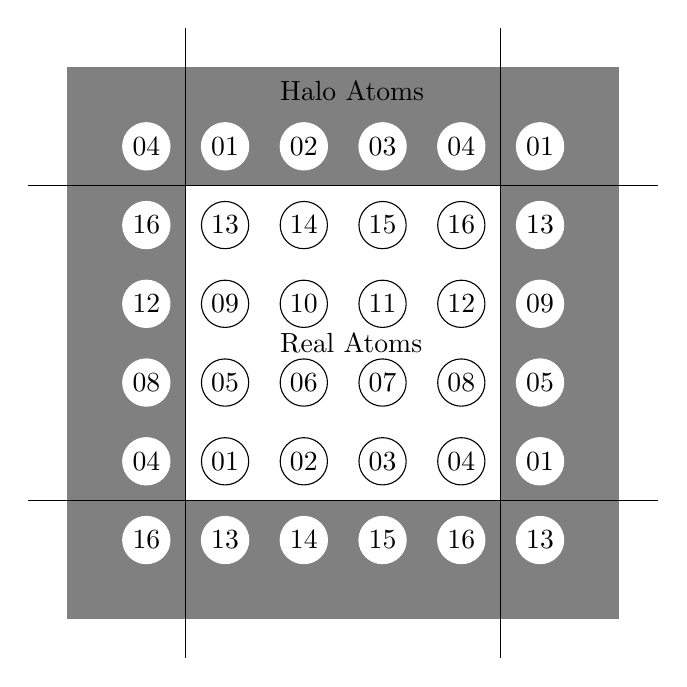
\begin{tikzpicture}
\filldraw [gray] (0.5,0.5) -- (0.5,7.5) -- (7.5,7.5) -- (7.5,0.5) -- (0.5,0.5);
\filldraw [white] (2.0,2.0) -- (2.0,6.0) -- (6.0,6.0) -- (6.0,2.0) -- (2.0,2.0);
\draw (0,2) -- (8,2);
\draw (0,6) -- (8,6);
\draw (2,0) -- (2,8);
\draw (6,0) -- (6,8);
\draw (2.5,2.5) circle [radius=0.3] node {$01$};
\draw (3.5,2.5) circle [radius=0.3] node {$02$};
\draw (4.5,2.5) circle [radius=0.3] node {$03$};
\draw (5.5,2.5) circle [radius=0.3] node {$04$};
\draw (2.5,3.5) circle [radius=0.3] node {$05$};
\draw (3.5,3.5) circle [radius=0.3] node {$06$};
\draw (4.5,3.5) circle [radius=0.3] node {$07$};
\draw (5.5,3.5) circle [radius=0.3] node {$08$};
\draw (2.5,4.5) circle [radius=0.3] node {$09$};
\draw (3.5,4.5) circle [radius=0.3] node {$10$};
\draw (4.5,4.5) circle [radius=0.3] node {$11$};
\draw (5.5,4.5) circle [radius=0.3] node {$12$};
\draw (2.5,5.5) circle [radius=0.3] node {$13$};
\draw (3.5,5.5) circle [radius=0.3] node {$14$};
\draw (4.5,5.5) circle [radius=0.3] node {$15$};
\draw (5.5,5.5) circle [radius=0.3] node {$16$};
\filldraw [white] (1.5,1.5) circle [radius=0.3] node [text=black] {$16$};
\filldraw [white] (1.5,2.5) circle [radius=0.3] node [text=black] {$04$};
\filldraw [white] (1.5,3.5) circle [radius=0.3] node [text=black] {$08$};
\filldraw [white] (1.5,4.5) circle [radius=0.3] node [text=black] {$12$};
\filldraw [white] (1.5,5.5) circle [radius=0.3] node [text=black] {$16$};
\filldraw [white] (1.5,6.5) circle [radius=0.3] node [text=black] {$04$};
\filldraw [white] (2.5,6.5) circle [radius=0.3] node [text=black] {$01$};
\filldraw [white] (3.5,6.5) circle [radius=0.3] node [text=black] {$02$};
\filldraw [white] (4.5,6.5) circle [radius=0.3] node [text=black] {$03$};
\filldraw [white] (5.5,6.5) circle [radius=0.3] node [text=black] {$04$};
\filldraw [white] (6.5,6.5) circle [radius=0.3] node [text=black] {$01$};
\filldraw [white] (6.5,2.5) circle [radius=0.3] node [text=black] {$01$};
\filldraw [white] (6.5,3.5) circle [radius=0.3] node [text=black] {$05$};
\filldraw [white] (6.5,4.5) circle [radius=0.3] node [text=black] {$09$};
\filldraw [white] (6.5,5.5) circle [radius=0.3] node [text=black] {$13$};
\filldraw [white] (6.5,1.5) circle [radius=0.3] node [text=black] {$13$};
\filldraw [white] (2.5,1.5) circle [radius=0.3] node [text=black] {$13$};
\filldraw [white] (3.5,1.5) circle [radius=0.3] node [text=black] {$14$};
\filldraw [white] (4.5,1.5) circle [radius=0.3] node [text=black] {$15$};
\filldraw [white] (5.5,1.5) circle [radius=0.3] node [text=black] {$16$};
\node[text width=3cm] at (4.7,7.2) {Halo Atoms};
\node[text width=3cm] at (4.7,4.0) {Real Atoms};
\end{tikzpicture}
\end{center}
\caption{A 2D representation of atoms in simulation box with a halo of atoms at the boundary}
\label{fig:nlatomshalo}
\end{figure}



To build the neighbour list a halo configuration is created such that it lies on top of the real atoms, but extends at least as far as the cut off radius on each side of the real simulation box (fig. \ref{fig:nlatomshalo}).  Periodic boundary conditions are used to construct the halo.

Once the halo list is computed, the neighbour list may also be computed by looping through the real atoms and halo atoms.  A simple pseudo coded sub routine is given (listing \ref{listing:halfneighbourlist}).

\FloatBarrier
\begin{lstlisting}[style=sFortran,caption={Simple subroutine for generating a half size neighbour list},label={listing:halfneighbourlist}]

! real_atoms - array holding coordinates of all real atoms
! halo_atoms - array holding coordinates of all halo atoms
! real_ids - unique id for each atom
! halo_ids - unique atom ids for halo atoms
! nlist_ids - array to store ids
! nlist_r - array to store separation

! Define the cutoff and counter start value
r_cut = 5.0
nl_counter = 1

! Calculate square
r_cut_sq = r_cut ** 2

! Loop over all real atoms
DO n_real = 1, real_atom_count
  ! Loop over all halo atoms
  DO n_halo = 1, halo_atom_count
    IF (real_ids(n_real) .LT. halo_ids(n_halo)) THEN
      r(1:3) = halo_atoms(n_halo, :) - real_atoms(n_real, :)
      r_sq = SUM(r(1:3) * r(1:3))
      IF (r_sq .LE. r_cut_sq) THEN          
        r_mag = sqrt(r_sq)          
        nlist_ids(nl_counter, 1) = real_ids(n_real)
        nlist_ids(nl_counter, 2) = halo_ids(n_halo)        
        nlist_r(nl_counter, 1) = r_mag
        nlist_r(nl_counter, 2:4) = r(1:3)/r_mag
        nl_counter = nl_counter + 1
      END IF
    END IF
  END DO
END DO 
\end{lstlisting}

The resulting list will contain unique a pair combinations; i.e. the pair atom 1 and atom 2 will only be recorded once, and not also as atom 2 and atom 1.

Many modern \acrshort{md} codes are designed to run on computers with many thousands of processor cores.  This leads to a choice of approaches, either to keep the configuration in shared memory and allow multiple processes to work on the same data, or break the data up, distributing it across various nodes.    

In the case of DL\_POLY a link-cell domain decomposition is used\cite{dlpolymanual}.  The supercell is divided up into subcells, and these must be at least the size of the cut-off radius.   Each processor will work on a geometric domain and these will only interact with their immediate neighbours.  The halo data for each subcell is only passed between processors before and after the calculation of the equations of motion of the atoms within each subcell.

\begin{figure}[!htbp]
  \begin{center}
    \includegraphics[width=.6\linewidth]{chapters/interatomic_potential_fitting/images/domain-decomp.png}
    \caption{Partitioning in \acrshort{lammps}\cite{lammpsdd}}
    \label{fig:lammpsdd}
  \end{center}
\end{figure}

This is also the approach used by the \acrshort{lammps} code.  The simulation is partitioned into either boxes where the density of atoms is uniform or tiles where there are regions with few or no atoms (fig. \ref{fig:lammpsdd}).  This ensures processors are evenly utilised.




\FloatBarrier
\subsubsection{Computing Total Energy}

The total energy of the system is the sum of the individual energies for the atoms in the simulation.  The type of atom (or pairs of atoms) will determine which function is used.

First, to compute the pair potentials:

\begin{itemize}
\item set the total energy of the system equal to zero
\item set the starting energy for each atom in the system to zero
\item loop through the atom pairs in the entire neighbour list
\item for each atom pair, A and B, use the known separation and the potential function to compute the potential energy on atom A due to B and vice versa
\item add this potential energy to both A and B
\item after looping through the neighbour list, add all the energies due to the pair potential to the total energy
\end{itemize}

For an EAM or 2BEAM potential, the densities and embedding energies must also be computed:

\begin{itemize}
\item set the electron density at the position of (for each) atom to zero
\item loop through the atom pairs in the entire neighbour list
\item for each atom pair, using the density function for the atom A, the density at atom B due to atom A will be calculated and added to the density at atom B
\item if the atoms are both of the same type the same density will be added to atom A due to atom B
\item if the atom types are different, using the density function for the atom B, the density at atom A due to atom B will be calculated and added to the density at atom A
\item following looping through the neighbour list, to calculate the densities at each atom, the list of atoms will be looped through
\item for each atom, the density value at the position of that atom, will be input into the appropriate embedding function to calculate the embedding portion of the energy
\item add all the embedding energies to the total energy of the system
\end{itemize}

For a 2BEAM potential, repeat the above procedure for the second group of density functions and embedding functions (do not repeat calculation of the pair potentials).


\subsubsection{Computing Forces on Atoms}

In order to calculate the forces on the atoms with an \acrshort{eam} or \acrshort{2beam} potential, the neighbour list and atom list will need to be looped through several times.  First, the pair potential and force due to the pair potential must be calculated by a complete loop through the neighbour list.  At the same time, the density at each atom location is also calculated.  The embedding energy may then be computed by looping through all the atoms and using the electron density at each atom to give the energy of the atom embedded in that density.  The third and final loop will run through the neighbour pairs in the neighbour list once more computing the force on each atom due to its embedding in the electron background.

\begin{equation}
\begin{split}
F^k_{pair} = -\sum \limits_{j=1, j \ne k}^{N} \frac{\partial V_{kj} (r_{kj}}{\partial r_{kj}} \frac{\vec{r}_{kj}}{\lvert\vec{r}_{kj}\lvert} \\
F^k_{embed} = -\sum \limits_{j=1, j \ne k}^{N} \left(\frac{\partial F}{\partial \rho_k} \frac{\partial \rho (r_{j})}{\partial r_{kj}} + \frac{\partial F}{\partial \rho_j} \frac{\partial \rho (r_{k})}{\partial r_{kj}} \right)  \frac{\vec{r_{kj}}}{r_{kj}}
\end{split}
\label{eq:computingForces}
\end{equation}

The force on each atom, due to surrounding atoms, may be split into two; force due to the pair potential, and the force due to the embedding of the atom (eq. \ref{eq:computingForces})\cite{dawbaskeseam}\cite{dlpolymanual}.


\subsubsection{Computing Stress}

The stress is to be calculated assuming the system is at 0K\cite{wikivirialstress} so the virial stress equation is eq. \ref{eq:eqVirialStress}.

\begin{equation}
\begin{split}
\tau_{ij} = \frac{1}{2 V} \sum_{k,l \in V} \left({x_i}^{(l)} - {x_i}^{(k)} \right) {f_j}^{(kl)}
\end{split}
\label{eq:eqVirialStress}
\end{equation}

Within the computer code, the individual force components between pairs of atoms are stored as well as an equal sized array of vectors representing their spatial separation.  Those pairs with one atom in the halo around the simulation box are used to calculate the stress on the simulation box.


\subsubsection{Pseudo Code for the Energy, Force and Stress Subroutine}

The calculation requires several arrays to temporarily store data.  The electron densities and gradients of the density function are stored for multiple groups of densities and embedding functionals.  The overall forces on each atoms also need to be stored as well as the force between pairs of atoms, as this is required to compute the virial stress.  The Fortran code to compute this is included in the appendix (section \ref{section:appendixenergyforcestress}) and a pseudocode in listing \ref{listing:efscalc} explains the process.

\begin{lstlisting}[style=sFortran,caption={Pseudo Code for Energy and Stress Force Calculation}, label={listing:efscalc}]

electron_density[1:n_atoms, 1:bands] = 0.0  ! electron density at each atom
energy = 0.0                                ! total energy
forces[:,:] = 0.0                           ! forces each atom, 3D
force_between_pairs[:,:] = 0.0              ! used to store force between pairs, for stress computation
stress[:,:] = 0.0D0

! LOOP 1 - Pair energy, force and calculate densities
DO n = 1, neighbour_count
  E = get_PairEnergy(atom_a, atom_b, r[n,:])
  F[:] = get_PairForce(atom_a, atom_b, r[n,:])

  ! Save energy
  energy = energy + E

  ! Save Force
  f[atom_a, :] = f[atom_a, :] - F[:]
  f[atom_b, :] = f[atom_b, :] + F[:]
  force_between_pairs[:,:] = force_between_pairs[:,:] - F[:]   // Used to calculate stress
  
  ! Loop through density bands
  DO band = 1, bands
    ! Electron density at A due to atom B
    electron_density[atom_a, band] = get_Density(atom_b, r)
  
    ! Electron density at B due to atom A
    electron_density[atom_b, band] = get_Density(atom_a, r)
  END DO
END DO

! LOOP 2 - Embedding energy
DO n = 1, atom_count
  ! Loop through density bands
  DO band = 1, bands
    energy = energy + get_EmbeddingEnergy(n, band)
  END DO
END DO

! LOOP 3 - Embedding force
DO n = 1, neighbour_count
  ! Loop through density bands
  DO band = 1, bands
    dgradA = get_DensityGradient(atom_b, r, band)
    dgradB = get_DensityGradient(atom_a, r, band)
    fgradA = get_EmbeddingGradient(atom_a, electron_density[atom_a, band])
    fgradB = get_EmbeddingGradient(atom_b, electron_density[atom_b, band])

    F[:] = (fgradA * dgradB + fgradB * dgradA) * r[n, :]

    f[atom_a, :) = f(atom_a, :) - F[:] 
    f(atom_a, :) = f(atom_a, :) + F[:] 
    
    force_between_pairs[n,:] = force_between_pairs[n,:] - F[:]   // Used to calculate stress
  END DO
END DO

! LOOP 4 STRESS
DO n = 1, neighbour_count
  ! Only compute if the second atom is in the halo 
  IF(nlisthalo(n))THEN  
    DO i = 1,3
      DO j = 1,3
        stress[i,j] = stress[i,j] + (r[n, i] * force_between_pairs[n,j])
      END DO
    END DO
  END IF
END DO
stress[1:3, 1:3] = stress[1:3, 1:3] / (2.0 * volume)

\end{lstlisting}




\subsection{Velocity Verlet Algorithm}

Verlet integration is used by \acrshort{md} codes such as DL\_POLY, \acrshort{lammps}, Democritus as well as \acrshort{md} \acrshort{dft} codes, as in the case of CASTEP.  

First, the forces at time step n are calculated $\vec{f_{n}}$.  Now, using these forces and the velocity at time step n, the half step velocity is computed (eq. \ref{eq:verlet1}).

\begin{equation}
\begin{split}
\vec{v_{n+half}} = \vec{v_{n}} + \frac{\vec{f_{n}} \delta t}{2 m}
\end{split}
\label{eq:verlet1}
\end{equation}

The position of the next step, n + 1, is calculated using the position at n, the time step $dt$ and the half step velocity (eq. \ref{eq:verlet2}).

\begin{equation}
\begin{split}
\vec{r_{n+1}} = \vec{r_{n}} + \vec{v_{n+half}} \times \delta t
\end{split}
\label{eq:verlet2}
\end{equation}

The forces are recalculated at the new position $\vec{r_{n+1}}$ to give $\vec{f_{n+1}}$ and this, along with the half step velocity, is used to compute the velocity at step n+1, $\vec{v_{n+1}}$ (eq. \ref{eq:verlet3}). 

\begin{equation}
\begin{split}
\vec{v_{n+1}} = \vec{v_{n+half}} + \frac{\vec{f_{n+1}} \delta t}{2 m}
\end{split}
\label{eq:verlet3}
\end{equation}

This process is repeated for each time step $\delta t$ from the start of the simulation to the end.  




\subsection{Selecting a Time Scale}

Take, for example, a 50x50x50 BCC Iron supercell with a lattice parameter of 2.87 angstrom.  The supercell measures almost 15nm on each side.  Simulating a thermal neutron, travelling at 2,200 m/s, would require an overall time period of at least 7 picosecond to capture the neutron passing through the supercell.  Higher energy particles would require smaller overall time periods, divided up into as many time steps as the user requires.  

If PKA damage is being modelled, there may be a point where the depth of the damage cascade becomes larger than the supercell itself.  Damage cascades of 500KeV iron atoms into an iron target travel to a depth of up to 300nm, which would require a simulation supercell at least 1,000 BCC cells deep.  Kinetic Monte Carlo would be better suited at simulating higher energy damage cascades.   

\begin{figure}[h]
  \begin{center}
    \includegraphics[width=.6\linewidth]{chapters/interatomic_potential_fitting/plots/fe500kev.png}
    \caption{Damage cascade: 500kev iron projectiles into an iron target calculated with SRIM}
    \label{graph:fe500kev}
  \end{center}
\end{figure}

To capture the required details the time steps would also need to be very fine, on the order of attoseconds or tens of attoseconds.  This has been shown in the literature with time steps of $7.8 \times 10^{-17}$s\cite{moxlammpsdamage}.




%%%%%%%%%%%%%%%%%%%%%%%%%%%%%%%%%%%%%%%%%%%%%%%%%%%%%%%%%%%%%%%%%%%%%%%%%%%%%%%%%%%%%%%%%%%%%%%%%%%%%%%%%%
%%
%%  KINETIC MONTE CARLO
%%
%%%%%%%%%%%%%%%%%%%%%%%%%%%%%%%%%%%%%%%%%%%%%%%%%%%%%%%%%%%%%%%%%%%%%%%%%%%%%%%%%%%%%%%%%%%%%%%%%%%%%%%%%%

%%\section{Kinetic Monte Carlo}






%%%%%%%%%%%%%%%%%%%%%%%%%%%%%%%%%%%%%%%%%%%%%%%%%%%%%%%%%%%%%%%%%%%%%%%%%%%%%%%%%%%%%%%%%%%%%%%%%%%%%%%%%%
%%
%%  OPTIMIZATION
%%
%%%%%%%%%%%%%%%%%%%%%%%%%%%%%%%%%%%%%%%%%%%%%%%%%%%%%%%%%%%%%%%%%%%%%%%%%%%%%%%%%%%%%%%%%%%%%%%%%%%%%%%%%%






%%%%%%%%%%%%%%%%%%%%%%%%%%%%%%%%%%%%%%%%%%%%%%%%%%%%%%%%%%%%%%%%%%%%%%%%%%%%%%%%%%%%%%%%%%%%%%%%%%%%%%%%%%
%%
%%  FITTING PROGRAMS
%%
%%%%%%%%%%%%%%%%%%%%%%%%%%%%%%%%%%%%%%%%%%%%%%%%%%%%%%%%%%%%%%%%%%%%%%%%%%%%%%%%%%%%%%%%%%%%%%%%%%%%%%%%%%


\section{Existing Potential Fitting Programs}
\label{section:fittingprograms}

\subsubsection{Bonny Quadratic Program Fitting}

This code has been used to fit a number of potentials, including Fe-Cr and W-Re.  It is a Fortran code and uses know properties of the material in different configurations.  The only functional forms available in the 2012 version of the code are cubic spline for the pair and density functions and a polynomial for the embedding functional.  The fitting subroutine uses quadratic programming to find parameters for the pair and embedding function splines.




\subsubsection{Hepburn FitPot}

FitPot was created by Hepburn, a co-author of papers with Ackland\cite{hepburnfec}.  It was written in Java and tackles the fitting as a non-linear least squares problem.  The \acrfull{lma} is used to minimise the response function and uses the derivatives of the response function with respect to the input parameters to construct the Jacobian that is then used to construct an estimation of the Hessian.


\subsubsection{Brommer PotFit}

Originally developed in C, the PotFit\cite{pbrommer} program uses the force matching method of fitting.  In the early versions of the code, splines were the only function choice available.  In the years since, the option to fit analytic functions has been added.  Simulated annealing is the primary search algorithm that attempts to locate the global minima.  Powell's conjugate direction method is used to locate the local minima once the probable global minima is located.  In order to use PotFit, a database of force, energy and stress for various configurations is required.


\subsubsection{Sheng Modified PotFit}
\label{section:shengeampotentials}

A set of potentials have been derived by Sheng et al\cite{shengeam} and are available to download in tabulated form\cite{shengeamonline}.   They were created using a modified version of the PotFit code by P. Brommer and F. G\"ahler\cite{pbrommer}.  The code had been modified extensively to include quintic spline interpolation, phonon calculation, elastic constant calculation and optimization techniques\cite{shengeamonline}.  The potentials (typically) used 15 knot splines for pair and density functions and 6 knot splines for the embedding functional for each element, but the potentials were published as tabulated functions.  Potentials for fourteen FCC metals were derived in the first instance, but more (including alloys) are available on the website.  Unfortunately, the (Sheng et al.) modified PotFit code is not available through the PotFit website\cite{pbrommer}, and the latest version of their code has moved on since 2011.





%%%%%%%%%%%%%%%%%%%%%%%%%%%%%%%%%%%%%%%%%%%%%%%%%%%%%%%%%%%%%%%%%%%%%%%%%%%%%%%%%%%%%%%%%%%%%%%%%%%%%%%%%%
%%
%%  DFT
%%
%%%%%%%%%%%%%%%%%%%%%%%%%%%%%%%%%%%%%%%%%%%%%%%%%%%%%%%%%%%%%%%%%%%%%%%%%%%%%%%%%%%%%%%%%%%%%%%%%%%%%%%%%%





\section{Density Functional Theory}

\Acrfull{dft} is a branch of quantum chemistry that approximately solves the Schr\"{o}dinger equation using electron density, rather than the coordinates of each electron in the system.  A number of simplifications are also applied in order for \acrshort{dft} to be practical to use, but despite this calculations are limited to just hundreds or thousands of atoms.  A calculation of a hundred or so atoms may take thousands of \acrshort{cpu} hours at the time of writing, depending on the type of calculation and complexity of the electron structures of the atoms involved.

It is through \acrshort{dft} that the first principles energy, stress and force calculations will be made, and it's these results that the EAM potentials will be trained and fit to using the force matching method.  This will allow much larger scale modelling using the extrapolated behaviour of accurate \acrshort{dft} calculations.



\FloatBarrier
\subsection{Motivation For Using \acrshort{dft} In This Work}

The use of interatomic potentials bridges the gap between the quantum scale and macroscopic scale.  In order to develop these potentials either measurements or calculated values are needed for forces, energies and stresses.  \acrshort{dft} is a convenient choice and has been used to fit potentials and calculate crystal properties many times (Sheng et al\cite{shengeam}, Mehl et al.\cite{mehlsp} Connetable and Thomes,\cite{orthonisi} Ravindran et al\cite{dftrfkj}, Hepburn and Ackland\cite{hepburnfec} and more).


\FloatBarrier
\subsection{Brief Overview of DFT}

Several important theories and approximations are used by \acrshort{dft} with the aim of calculating and minimising energies and forces.  The Born-Oppenheimer approximation separates the electron-nucleus wave function.  It treats the nuclei as fixed points, and the system of electrons in a fixed potential created by the nuclei.


The \acrshort{dft} of Kohn, Sham and Hohenburg proved that the potential of a system is uniquely determined by its ground state density.  This makes solving the Schr\"{o}dinger equation significantly easier.

\begin{figure}[!h]
\centering
\resizebox{0.4\textwidth}{!}{%
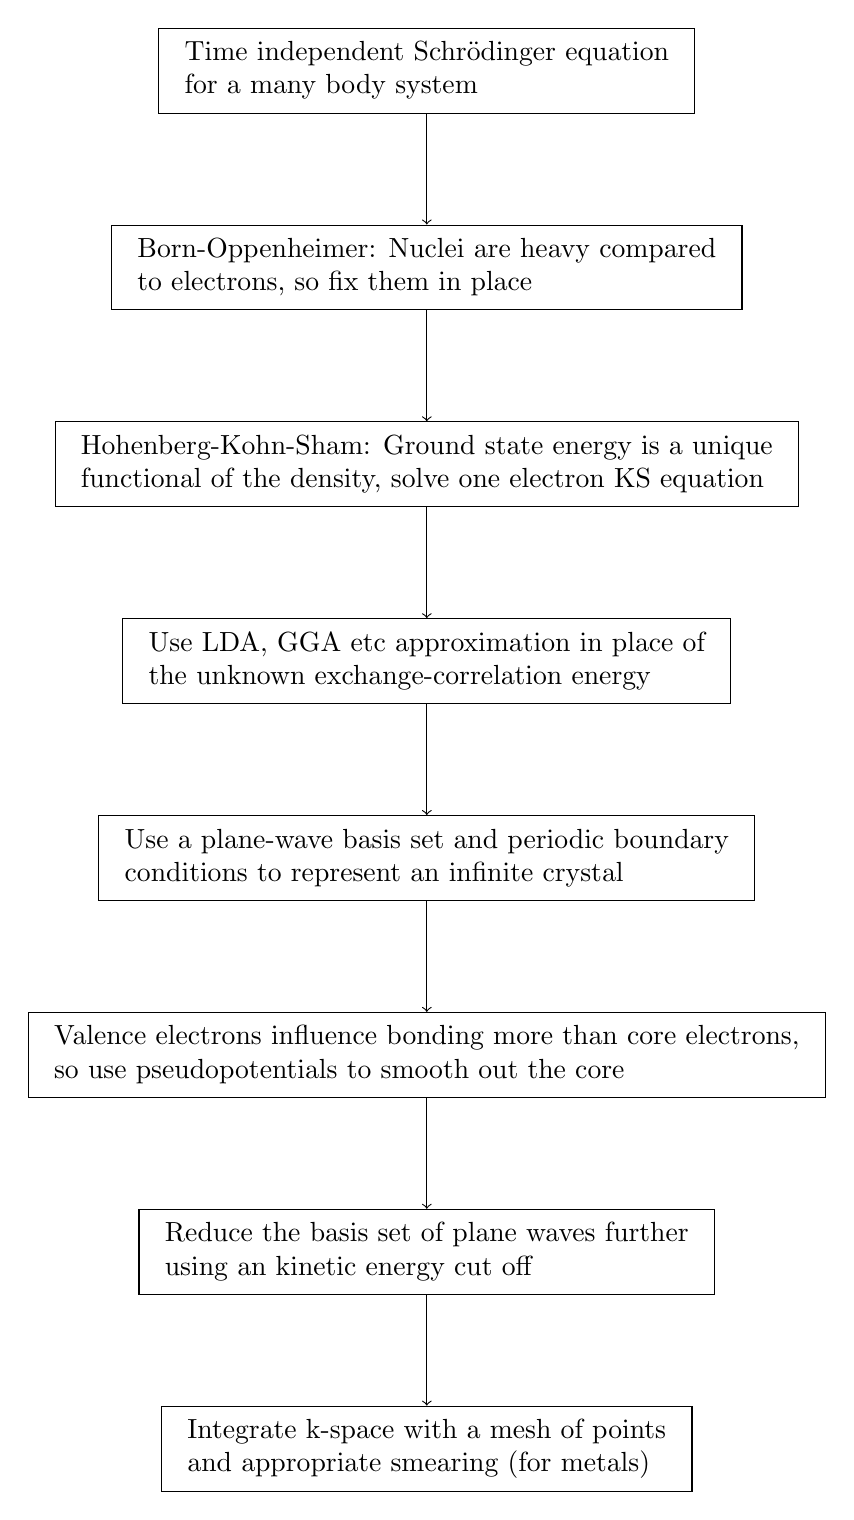
\begin{tikzpicture}[node distance=2.5cm]
\node (a) [rectangle, draw, fill=none] {\begin{tabular}{l}
Time independent Schr\"{o}dinger equation \\
for a many body system
\end{tabular}};
\node (b) [rectangle, draw, fill=none, below of=a] {\begin{tabular}{l}
Born-Oppenheimer: Nuclei are heavy compared \\
to electrons, so fix them in place
\end{tabular}};
\node (c) [rectangle, draw, fill=none, below of=b] {\begin{tabular}{l}
Hohenberg-Kohn-Sham: Ground state energy is a unique \\
functional of the density, solve one electron KS equation
\end{tabular}};
\node (d) [rectangle, draw, fill=none, below of=c] {\begin{tabular}{l}
Use LDA, GGA etc approximation in place of \\
the unknown exchange-correlation energy
\end{tabular}};
\node (e) [rectangle, draw, fill=none, below of=d] {\begin{tabular}{l}
Use a plane-wave basis set and periodic boundary \\
conditions to represent an infinite crystal
\end{tabular}};
\node (f) [rectangle, draw, fill=none, below of=e] {\begin{tabular}{l}
Valence electrons influence bonding more than core electrons, \\
so use pseudopotentials to smooth out the core
\end{tabular}};
\node (g) [rectangle, draw, fill=none, below of=f] {\begin{tabular}{l}
Reduce the basis set of plane waves further \\
using an kinetic energy cut off
\end{tabular}};
\node (h) [rectangle, draw, fill=none, below of=g] {\begin{tabular}{l}
Integrate k-space with a mesh of points \\
and appropriate smearing (for metals)
\end{tabular}};
%% arrows
\draw [->] (a) -- (b);
\draw [->] (b) -- (c);
\draw [->] (c) -- (d);
\draw [->] (d) -- (e);
\draw [->] (e) -- (f);
\draw [->] (f) -- (g);
\draw [->] (g) -- (h);
\end{tikzpicture}
}%
\caption{Common approximations used to enable \acrshort{dft} calculations}
\label{fig:dftapproximations}
\end{figure}








\FloatBarrier
\subsection{\acrlong{tise}}

The Schr\"{o}dinger equation is a linear partial differential wave equation and it was proposed by Erwin Schr\"{o}dinger in 1925.  There is a time-dependent and time-independent form of the equation.  As the \acrshort{dft} calculations in this work are static only the time-independent version will be discussed.  

\begin{equation}
\begin{split}
\hat{H} \lvert \Psi \rangle = E \lvert \Psi \rangle
\end{split}
\label{eq:eqTimeIndependentSchrodinger}
\end{equation}

The \Gls{hamiltonian} $\hat{H}$ is an operator and it is the total energy in the system.  $\Psi$ is the \gls{wavefunction} and this contains all the measurable information possible about whatever it represents.  E is the energy eigenvalue of this system and this will depend on the eigenstate of the system.  The wave function is also connected to the probability of a particle being found at a certain point in space, and the integral over all space is equal to 1 i.e. the probability of it being found somewhere in space is equal to 1 (eq. \ref{eq:foundsomewhere}).

\begin{equation}
\begin{split}
\int_{-\infty}^{\infty} \int_{-\infty}^{\infty}  \int_{-\infty}^{\infty}  \Psi(x,y,z) dx dy dz = 1
\end{split}
\label{eq:foundsomewhere}
\end{equation}

The Schr\"{o}dinger equation is set up depending on the system being studied.  Starting with the simplest, a free particle, the only non zero energy of the Hamiltonian is kinetic.


\begin{equation}
\begin{split}
\hat{H} = \frac{\hbar^2}{2 m} \nabla^2 \\
-\frac{\hbar^2}{2 m} \nabla^2 \Psi(\vec{r}) = E \Psi(\vec{r})
\end{split}
\label{eq:eqTimeIndependentSchrodinger1}
\end{equation}

If the particle is in a potential, it will have both kinetic energy $\hat{T}$ and potential energy $\hat{V}$ (eq. \ref{eq:eqTimeIndependentSchrodinger2}).

\begin{equation}
\begin{split}
\hat{H} = \hat{T} + \hat{V} = \frac{\hbar^2}{2 m} \nabla^2 + V(\vec{r})\\
\left[-\frac{\hbar^2}{2 m} \nabla^2 \right] \Psi(\vec{r}) = E \Psi(\vec{r})
\end{split}
\label{eq:eqTimeIndependentSchrodinger2}
\end{equation}




\subsection{Many Body \acrshort{tise}}

Electronic structure calculations are important and allow the calculation of material properties that may be difficult or impossible to measure with current technology.  The next step towards this is to set up the Schr\"{o}dinger equation (time-independent) for nuclei and electrons in a crystal.  

Relative to the strong force, the electromagnetic force is 1/137th as strong, but the strong force acts over a range of approximately $1.0 \times 10^{-5}$ angstrom.  In the calculations carried out in this section, the atoms will never be arranged close enough for the strong force to be considered at all.  The gravitational force, as with the electromagnetic force, acts over an infinite range.  The electromagnetic force is more than $1.0 \times 10^{36}$ times greater than the gravitational force, so it too can be neglected.  Finally, the weak interacting force has a range of approximately $1.0 \times 10^{-8}$ angstrom which, as with the strong force, is a range small enough that the weak force may be neglected.

The energy operators required are kinetic and electromagnetic potential (eq. \ref{eq:eqTimeIndependentSchrodinger3}).

\begin{equation}
\begin{split}
\hat{H} = \hat{T_e} + \hat{T_n} + \hat{V_{e-e}} + \hat{V_{e-n}} + \hat{V_{n-n}}
\end{split}
\label{eq:eqTimeIndependentSchrodinger3}
\end{equation}

The first two terms are the kinetic energy of the electrons and nuclei respectively (eq. \ref{eq:eqTimeIndependentSchrodinger4}).

\begin{equation}
\begin{split}
\hat{T_e} = - \sum_{i} \frac{\hbar^2}{2 m}  \nabla^2 \text{  sum of kinetic energy of electrons} \\
\hat{T_n} = - \sum_{k} \frac{\hbar^2}{2 M}  \nabla^2 \text{  sum of kinetic energy of nuclei}
\end{split}
\label{eq:eqTimeIndependentSchrodinger4}
\end{equation}

The last three terms are potential energy terms due to the electromagnetic force (eq. \ref{eq:eqTimeIndependentSchrodinger5}). 

\begin{equation}
\begin{split}
V_{e-e} = \frac{1}{2} \sum_{i,j,i \neq j} \frac{1}{\abs{\vec{r}_i - \vec{r}_j}} \text{  sum of potential energy between electrons} \\
V_{e-n} = \sum_{i,k} \frac{z_i}{\abs{\vec{r}_i - \vec{r}_l}} \text{  sum of potential energy between electrons and nuclei} \\
V_{n-n} = \frac{1}{2} \sum_{k,l,k \neq l} \frac{z_k z_l}{\abs{\vec{r}_l - \vec{r}_k}} \text{  sum of potential energy between nuclei}
\end{split}
\label{eq:eqTimeIndependentSchrodinger5}
\end{equation}

These operators are now input into the \acrshort{tise} (eq. \ref{eq:eqTimeIndependentSchrodinger6}).


\begin{equation}
\begin{split}
\left[ \left(- \sum_{i} \frac{\hbar^2}{2 m} - \sum_{k} \frac{\hbar^2}{2 M} \right) \nabla^2  + \sum_{i,k} \frac{z_i}{\abs{\vec{r}_i - \vec{r}_l}} + \frac{1}{2} \left( \sum_{i,j,i \neq j} \frac{1}{\abs{\vec{r}_i - \vec{r}_j}} + \sum_{k,l,k \neq l} \frac{z_k z_l}{\abs{\vec{r}_l - \vec{r}_k}} \right) \right] \lvert \Psi \rangle = E \lvert \Psi \rangle
\end{split}
\label{eq:eqTimeIndependentSchrodinger6}
\end{equation}



\subsection{Born-Oppenheimer}

The \acrshort{tise} arrived at is far too complicated to solve, even for the simple ensembles of atoms.  It represents the many body system of electrons and nuclei, and it takes the positions of all nuclei and electrons as input variables (eq. \ref{eq:eqTimeIndependentSchrodinger7}).

\begin{equation}
\begin{split}
\hat{H} \lvert \Psi (\vec{r_e}, \vec{r_n}) \rangle = E \lvert \Psi (\vec{r_e}, \vec{r_n}) \rangle \\
\text{ where } \vec{r_e} = r_{e,1}, r_{e,1},...,r_{e,i} \text{ (electron positions)} \\
\text{ where } \vec{r_n} = r_{n,1}, r_{n,1},...,r_{n,i} \text{ (electron positions)} \\
\end{split}
\label{eq:eqTimeIndependentSchrodinger7}
\end{equation}

In 1927 the Born-Oppenheimer approximation was proposed to separate the electron components from the nuclei in the Hamiltonian.  

Protons and neutrons are almost 2,000 times the mass of electrons.  With respect to the electrons, they move much slower and may be considered to be fixed or frozen in place.  Simplifying for a moment to a single electron and proton, due to Newton's second law, we can see that the acceleration of the electron would be similarly 2,000 times that of the proton: $f_e = f_p$ and $m_e a_e = m_p a_p$ which leads to $a_e = \frac{m_p}{m_e} a_p$.  As the nuclei move, the electrons are assumed to respond instantly, remaining in the ground state and not being promoted into higher energy levels.

The Hamiltonian for the electrons may be written with the electron co-ordinates as a variable, and the nuclei co-ordinates as a parameter (eq. \ref{eq:eqTimeIndependentSchrodinger8}).

\begin{equation}
\begin{split}
\hat{H_e} (\vec{r_e}; \vec{r_n}) = \hat{T_e}(\vec{r_e}) + \hat{V_{e-e}}(\vec{r_e}) + \hat{V_e-n}(\vec{r_e}; \vec{r_n})
\end{split}
\label{eq:eqTimeIndependentSchrodinger8}
\end{equation}

The wavefunction and energy for the electrons may be calculated, although if the nuclear cooridinates are changed, i.e. by changing the parameter $r_n$, the wavefucntion and energy will need to be recalculated.

\begin{equation}
\begin{split}
\hat{H_e} (\vec{r_e}; \vec{r_n}) \psi_{e} (\vec{r_e}; \vec{r_n}) = E_e (\vec{r_n})  \psi_{e} (\vec{r_e}; \vec{r_n}) 
\end{split}
\label{eq:elechamiltonian}
\end{equation}


\begin{equation}
\begin{split}
\Psi (\vec{r_e}, \vec{r_n}) = \chi_{ne} (\vec{r_e}) \psi_{e} (\vec{r_e}; \vec{r_n})
\end{split}
\label{eq:combinedwavefunction}
\end{equation}

The electronic Hamiltonian (eq. \ref{eq:elechamiltonian}) is still dependent on the electronic co-ordinates.  As there are three co-ordinates per electron, there are 3 dimensions when solving for a hydrogen atom.  For an Iron atom, with 26 electrons, there are 78 dimensions, and for a 4x4x4 FCC supercell of Iron there would be 256 atoms, 26 electrons per atom and 3 dimensions per electon, giving a total of 19,968 dimensions.  Even for small numbers of electrons, solving this equation is impractical.




\subsection{Crystals, Reciprocal Space and Bloch Theorem}
\label{section:crystalsrecipbloch}

A Bravais lattice is a construct used to describe a periodic crystal lattice.  It has the following properties given in eq. \ref{eq:reciprocalspace}. 

\begin{equation}
  \begin{split}
    \vec{R} = n_1 \vec{a}_1 + n_2 \vec{a}_2 + n_3 \vec{a}_3 \\
    n_1 , n_2, n_3 \in Z \\
    \vec{a}_1, \vec{a}_2, \vec{a}_3 \text{ are independent}
  \end{split}
  \label{eq:reciprocalspace}
\end{equation}

There are 14 Bravais lattices and 7 families of these lattices, and these lattices may be grouped by vector length and angle relationships (table. \ref{table:bravaisvectors}).  This work is primarily concerned with cubic and tetragonal crystals, although distortions are applied to these crystals throughout.

\begin{table}[h]
\begin{center}
\renewcommand{\arraystretch}{1.2}
\begin{tabular}{c c c}
\hline\hline
Class & Lengths & Angles \\
\hline\hline
Cubic & $a = b = c$ & $ \alpha = \beta = \gamma = 90 $ \\
Hexagonal & $a = b, c $ & $ \alpha = \beta, \gamma = 120 $ \\
Rhombohedral & $a = b = c $ & $ \alpha = \beta = \gamma \neq 90 $ \\
Tetragonal & $a = b, c $ & $ \alpha = \beta = \gamma = 90 $ \\
Orthorhombic & $a, b, c $ & $ \alpha = \beta = \gamma = 90 $ \\
Monoclinic & $a, b, c $ & $ \alpha = \beta = 90, \gamma \neq 90 $ \\
Triclinic & $a, b, c $ & $ \alpha, \beta, \gamma, $ \\
\hline
\end{tabular}
\caption{Bravais lattice vector length and angle relationships}
\label{table:bravaisvectors}
\end{center}
\end{table}



\subsubsection{Bloch Theorem}
\label{section:blochtheorem}

Metals are made up from grains which in turn are crystal lattices of atoms.  Despite the majority of metals being composed of a large collection of microscopic crystals, rather than being a single perfect crystal, most of their properties may be calculated as if the metal were a single crystal.

The grain size of water quenched SS304 is approximately 30 micrometers across\cite{grainsizesteel}.  If the crystal were a cube, it would contain $2.0 \times 10^{15}$ atoms and it would have sides over 100,000 atoms in length.

In solid state physics, in order to solve the \acrshort{tise} for such a system, it is useful to consider an infinite sized crystal.  It may be helpful to visualise this as a "ring" of atoms in one dimension (fig. \ref{image:1dchainofatoms}) or as a super-cell with periodic boundary conditions in three dimensions.


\begin{figure}[htbp]
\begin{center}
\begin{minipage}{.47\textwidth}
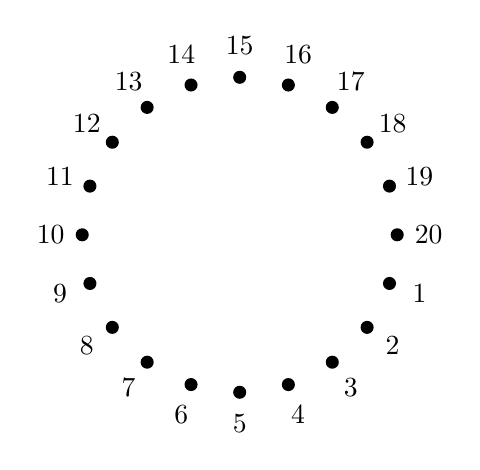
\begin{tikzpicture}
    % equidistant points and arc
    \foreach \x [count=\p] in {0,...,19} {
        \node[shape=circle,fill=black, scale=0.5] (\p) at (-\x*18:2) {};};
    \foreach \x [count=\p] in {1,...,20} {
        \draw (-\x*18:2.4) node {\p};}; 
\end{tikzpicture}
\caption{A useful, albeit incorrect, way of visualising an "infinite" chain of atoms in 1D}
\label{image:1dchainofatoms}
\end{minipage}
\begin{minipage}{.05\textwidth}
\end{minipage}
\begin{minipage}{.47\textwidth}

\begin{tikzpicture}
\tikzdrawline{col_000000}{0}{0}{0}{1}{0}{6}
\tikzdrawline{col_000000}{2}{0}{0}{3}{0}{6}
\tikzdrawline{col_000000}{4}{0}{0}{5}{0}{6}
\tikzdrawline{col_000000}{6}{0}{0}{7}{0}{6}
\tikzdrawline{col_000000}{8}{0}{0}{9}{0}{6}
\tikzdrawline{col_000000}{0}{0}{0}{8}{0}{0}
\tikzdrawline{col_000000}{0.333333}{0}{2}{8.33333}{0}{2}
\tikzdrawline{col_000000}{0.6666}{0}{4}{8.66666}{0}{4}
\tikzdrawline{col_000000}{1}{0}{6}{9}{0}{6}

\tikzdrawlinedotted{col_000000}{1.0}{0}{6}{1.1}{0}{6.5}
\tikzdrawlinedotted{col_000000}{3.0}{0}{6}{3.1}{0}{6.5}
\tikzdrawlinedotted{col_000000}{5.0}{0}{6}{5.1}{0}{6.5}
\tikzdrawlinedotted{col_000000}{7.0}{0}{6}{7.1}{0}{6.5}
\tikzdrawlinedotted{col_000000}{9.0}{0}{6}{9.1}{0}{6.5}

\tikzdrawlinedotted{col_000000}{-0.1}{0}{-0.5}{0.0}{0}{0}
\tikzdrawlinedotted{col_000000}{1.9}{0}{-0.5}{2}{0}{0}
\tikzdrawlinedotted{col_000000}{3.9}{0}{-0.5}{4}{0}{0}
\tikzdrawlinedotted{col_000000}{5.9}{0}{-0.5}{6}{0}{0}
\tikzdrawlinedotted{col_000000}{7.9}{0}{-0.5}{8}{0}{0}

\tikzdrawlinedotted{col_000000}{-0.5}{0}{0}{0.0}{0}{0}
\tikzdrawlinedotted{col_000000}{-0.22222}{0}{2}{0.3333}{0}{2}
\tikzdrawlinedotted{col_000000}{0.11111}{0}{4}{0.6666}{0}{4}
\tikzdrawlinedotted{col_000000}{0.5}{0}{6}{1.0}{0}{6}

\tikzdrawlinedotted{col_000000}{8}{0}{0}{8.5}{0}{0}
\tikzdrawlinedotted{col_000000}{8.3333}{0}{2}{8.83333}{0}{2}
\tikzdrawlinedotted{col_000000}{8.6666}{0}{4}{9.1666}{0}{4}
\tikzdrawlinedotted{col_000000}{9.0}{0}{6}{9.5}{0}{6}

\tikzdrawlinethick{col_000000}{0}{0}{0}{0.333}{0}{2}
\tikzdrawlinethick{col_000000}{2}{0}{0}{2.333}{0}{2}
\tikzdrawlinethick{col_000000}{0}{0}{0}{2}{0}{0}
\tikzdrawlinethick{col_000000}{0.3333}{0}{2}{2.333}{0}{2}

\tikzdrawlinethick{col_000000}{4.3333}{0}{2}{4.6666}{0}{4}
\tikzdrawlinethick{col_000000}{6.3333}{0}{2}{6.6666}{0}{4}
\tikzdrawlinethick{col_000000}{4.3333}{0}{2}{6.3333}{0}{2}
\tikzdrawlinethick{col_000000}{4.6666}{0}{4}{6.6666}{0}{4}

\tikzdrawline{col_000000}{1.1}{0}{2}{1.33333}{0}{3}
\tikzdrawarrow{col_000000}{1.33333}{0}{3}{4.45}{0}{3}{above}{$\vec{R}$}

\node[] at (1.1,1.0) {$\vec{r}$};
\node[] at (5.5,3.0) {$\vec{r} + \vec{R_{t}}$};
\end{tikzpicture}
\caption{A 2D example of a translation by an integer multiple of the unit cell from the origin unit cell}
\label{image:2dtranslation}

\end{minipage}
\end{center}
\end{figure}




\FloatBarrier
As the structure is a repeating lattice, any point within a unit cell is equivalent to any other point translated by an integer multiple of the lattice vector (fig. \ref{image:2dtranslation}).

\begin{equation}
  \begin{split}
    \psi(\vec{r}) = \psi(\vec{r} + \vec{R_t}) \\
    \text{where } \vec{R_t} = n_1 \vec{R}_{1} + n_2 \vec{R}_{2} + n_3 \vec{R}_{3} \\
    \text{where } \vec{R} \text{ is the real lattice vector}
  \end{split}
  \label{eq:eqEulersFormula}
\end{equation}


Reciprocal space, also known as k-space or momentum space, is a mathematical construct.  It is an imaginary space where the lengths, and volumes, are the inverse of real space and planes of atoms are represented as points. 

%\begin{figure}[htbp]
%\begin{center}
%\begin{minipage}{.4\textwidth}
%\begin{tikzpicture}
%\tikzcoordgrid{4.0}{4.0}{4.0}{$\vec{a_1}$}{$\vec{a_1}$}{$\vec{a_1}$}
%\end{tikzpicture}
%\end{minipage}
%\begin{minipage}{.1\textwidth}
%\end{minipage}
%\begin{minipage}{.4\textwidth}
%\begin{tikzpicture}
%\tikzcoordgrid{4.0}{4.0}{4.0}{$\vec{b_1}$}{$\vec{b_1}$}{$\vec{b_1}$}
%\end{tikzpicture}
%\end{minipage}
%\caption{Graph caption}
%\label{graph:graph1}
%\end{center}
%\end{figure}

Starting with a lattice of points in real space $\vec{R}$, points in reciprocal space $\vec{G}$ only are valid points if $\exp(i \vec{G} \cdot \vec{R}) = 1$\cite{solidstatebasics}.  A real space vector $\vec{R}$ is transformed to it's reciprocal in the following way, where $\Omega$ is the volume of the primitive cell in real space.

\begin{equation}
  \begin{split}
    \vec{g_1} = \frac{2 \pi}{\Omega} \vec{r_2} \times \vec{r_3} \\
    \vec{g_2} = \frac{2 \pi}{\Omega} \vec{r_3} \times \vec{r_1} \\
    \vec{g_3} = \frac{2 \pi}{\Omega} \vec{r_1} \times \vec{r_2} \\
    \Omega = \vec{r_1} \cdot (\vec{r_2} \times \vec{r_3}) \\
  \end{split}
  \label{eq:eqReciprocalLattice}
\end{equation}

If the crystal structure is modelled as an infinitely repeating lattice, the potential also has the same periodicity (eq. \ref{eq:eqReciprocalLattice}).

\begin{equation}
  \begin{split}
    V(\vec{r}) = V(\vec{r} + \vec{R}_{t}) 
  \end{split}
  \label{eq:eqPeriodicPotential1}
\end{equation}

As the potential is a periodic function, it may be written as a fourier series in reciprocal space (eq. \ref{eq:eqPeriodicPotentialSeries1}).

\begin{equation}
  \begin{split}
    V(\vec{r}) = \sum_{\vec{G}} V_{\vec{G}} \exp(i \vec{G} \cdot \vec{r})
  \end{split}
  \label{eq:eqPeriodicPotentialSeries1}
\end{equation}

The wave function for an electron in the lattice is also periodic and may be written as the product of a \gls{planewave}.   

\begin{equation}
  \begin{split}
    \psi_{n\vec{k}} (\vec{r}) = u_{n\vec{k}}(\vec{r}) \exp(i \vec{k} \cdot \vec{r})
  \end{split}
  \label{eq:eqPeriodicPotentialSeries2}
\end{equation}

\begin{equation}
  \begin{split}
    u_{n\vec{k}}(\vec{r}) = u_{n\vec{k}}(\vec{r} + \vec{R_{t}}) \\
     \psi_{n\vec{k}} (\vec{r}) = \psi_{n\vec{k}} (\vec{r}) \exp(i \vec{k} \cdot \vec{R_{t}}) \\
  \end{split}
  \label{eq:eqPeriodicPotentialSeries3}
\end{equation}

The Born-von Karman boundary conditions apply to the wave function such that:

\begin{equation}
  \begin{split}
    \psi_{n\vec{k}} (\vec{r} + \vec{R}_{t}) = \psi_{n\vec{k}} (\vec{r}) \
    \text{where} \vec{R_t} = \sum_i N_i \vec{a_i} \
    \text{and} N_i \in \mathbb{Z}
  \end{split}
  \label{eq:eqPeriodicPotentialSeries4}
\end{equation}

With these boundary conditions and use of plane waves, \Gls{blochtheorem} replaces an enormous number of electrons with an infinite number electrons in a periodic lattice where only those in the unit cell need to be considered.

\FloatBarrier
\begin{figure}[!htb]
\minipage{0.49\textwidth}
\includegraphics[width=\linewidth]{chapters/interatomic_potential_fitting/images/bcc_wcs_bz.png}
\caption{BCC Wigner Seitz Cell and \acrshort{bz} \cite{fccbccreciprocal}}
\label{fig:bccrecip}
\endminipage\hfill
\minipage{0.49\textwidth}
\includegraphics[width=\linewidth]{chapters/interatomic_potential_fitting/images/fcc_wcs_bz.png}
\caption{FCC Wigner Seitz Cell and \acrshort{bz} \cite{fccbccreciprocal}}
\label{fig:fccrecip}
\endminipage
\end{figure}
\FloatBarrier

The (first) \Gls{brillouinzone} is a volume in (3D) reciprocal space and it is analogous to the \Gls{wignerseitzcell} in real space.  It is the primitive lattice cell in reciprocal space.  The reciprocal of a \acrshort{bcc} lattice is a \acrshort{fcc} lattice (fig. \ref{fig:bccrecip}) and vice versa (fig. \ref{fig:fccrecip}).  In real space a point anywhere in the lattice is a integer multiple of the lattice vector away from the same point in the origin \Gls{wignerseitzcell}.  There are an infinite number of wave vectors $\vec{k}$ in reciprocal space, but by virtue of the periodicity of the lattice, they are also all found within the Brillouin Zone.  If the crystal has symmetries, the \acrshort{bz} may be reduced further to the \acrlong{ibz}.

Within the \acrshort{bz} there are energy surfaces.  Picking a straight line through reciprocal space allows one to plot the energy bands along that one dimensional space.  A particularly important energy surface is the Fermi surface and, in the one electron model, this marks the boundary between the occupied and unoccupied states at 0K \cite{hjonesfermi}.  The \Gls{fermienergy} is the energy of the highest occupied state at 0K.



\subsection{\Acrlong{hk} Theorem}

In the 1960s, Hohenberg and Kohn\cite{hohenbergkohn} simplified the problem of solving the many electron \acrshort{tise} in an exact way by proving:

\begin{itemize}
\item in an external potential $v(\vec{r})$, the potential is uniquely determined by the density of the ground state $n_0(\vec{r})$ assuming that the particles are non-degenerate
\item a uniquely defined functional $E[\rho(\vec{r})]$ exists and the ground state energy, $min(E[\rho(\vec{r})])$, is found by varying the density
\end{itemize}

The proof starts by picturing a box of electrons that interact with each other through coulomb repulsion within an external potential  $\vec{v}(r)$, for example the potential of \enquote{fixed} nuclei following the Born Oppenheimer approximation.

\begin{equation}
\begin{split}
\hat{H} = \hat{T} + \hat{V} = \frac{1}{2} \nabla^2 + V(\vec{r})\\
\left[-\frac{1}{2} \nabla^2 \right] \Psi(\vec{r})_{0} = E_{0} \Psi(\vec{r})
\end{split}
\label{eq:eqtishk}
\end{equation}

\begin{equation}
\begin{split}
\hat{H} = \hat{T} + \hat{V} + \hat{U}
\end{split}
\label{eq:eqHKhamiltonian}
\end{equation}

where

\begin{equation}
\begin{split}
T = \frac{1}{2} \int \nabla \psi^{*}(\vec{r})\nabla \psi(\vec{r}) d\vec{r}
\end{split}
\label{eq:eqHKKinetic}
\end{equation}

\begin{equation}
\begin{split}
V = \int v(\vec{r}) \psi^{*}(\vec{r}) \psi (\vec{r}) d\vec{r} 
\end{split}
\label{eq:eqHKexternal}
\end{equation}

\begin{equation}
\begin{split}
U = \frac{1}{\lvert \vec{r} - \vec{r}' \rvert} \psi^{*}(\vec{r}) \psi^{*}(\vec{r'}) \psi(\vec{r}) \psi(\vec{r}') d\vec{r} d\vec{r'}
\end{split}
\label{eq:eqHKinteraction}
\end{equation}

In the eqs. \ref{eq:eqHKhamiltonian} \ref{eq:eqHKKinetic} \ref{eq:eqHKhamiltonian} \ref{eq:eqHKinteraction} the hamiltonian operator $\hat{H}$ is a sum of the kinetic energy $\hat{T}$, the mutual coulomb repulsion $\hat{U}$ and the operator due to an external potential (due to the nuclei) $\hat{V}$.  The non degenerate ground state electron density is $n(\vec{r}) = \langle \Phi \lvert \phi^{*}(\vec{r}) \phi(\vec{r}) \rvert \Phi \rangle$.

The \acrshort{hk} theorem shows that the external potential $v(\vec{r})$ is a unique functional of the electron density $n(\vec{r})$.  The proof is that by contradiction where by two different states are assumed to have the same ground state charge density.


\minipage{0.49\textwidth}
\centering
\textbf{State A} \\
$\Psi_{A}$ with potential $V_A(\vec{r})$ \\
Hamiltonian $\hat{H} = \hat{T} + \hat{V_A} + \hat{U}$ \\
\acrshort{tise} $\hat{H_A} \Psi_A = E_A \Psi_A$\\
Assumption - this state has the charge density $n(\vec{r})$
\endminipage
\minipage{0.49\textwidth}
\centering
\textbf{State B} \\
$\Psi_{B}$ with potential $V_B(\vec{r})$ \\
Hamiltonian $\hat{H} = \hat{T} + \hat{V_B} + \hat{U}$ \\
\acrshort{tise} $\hat{H_B} \Psi_B = E_B \Psi_B$\\
Assumption - this state has the charge density $n(\vec{r})$
\endminipage

The minimal property of the ground state gives the following\cite{hohenbergkohn}\cite{hohenbergkohnleeuwen}:

\begin{equation}
\begin{split}
E_A = \langle \Phi_A \lvert \hat{H_A} \rvert \Phi_A \rangle \\
E_A = \langle \Phi_A \lvert \hat{H_B} + \hat{V_A} - \hat{V_B} \rvert \Phi_A \rangle \\
E_A = \langle \Phi_A \lvert \hat{H_B} \rvert \Phi_A \rangle + \int d^3 \vec{r} n(\vec{r})(v_A(\vec{r}) - v_B(\vec{r})) \\
\end{split}
\label{eq:minimalproperty}
\end{equation}

\begin{equation}
\begin{split}
E_A > E_B + \int d^3 \vec{r} n(\vec{r})(v_A(\vec{r}) - v_B(\vec{r}))
\end{split}
\label{eq:minimalproperty1}
\end{equation}

The indices A and B are interchanged to give a second equation:

\begin{equation}
\begin{split}
E_B > E_A + \int d^3 \vec{r} n(\vec{r})(v_B(\vec{r}) - v_A(\vec{r})) \\
E_B > E_A - \int d^3 \vec{r} n(\vec{r})(v_A(\vec{r}) + v_B(\vec{r}))
\end{split}
\label{eq:minimalproperty2}
\end{equation}

By adding eq. \ref{eq:minimalproperty1} and eq. \ref{eq:minimalproperty2} together the integrals will cancel out.

\begin{equation}
\begin{split}
E_A + E_B > E_A + E_B
\end{split}
\label{eq:hkcontradiction}
\end{equation}

This (eq. \ref{eq:hkcontradiction}) is a contradiction and proves the first part of the \acrshort{hk} theorem: $v(\vec{r})$ is uniquely determined by $n(\vec{r})$.  If the charge density (fig. \ref{fig:cdalfcc1} and \ref{fig:cdalfcc1}) is known, a single external potential exists for it.

\FloatBarrier
\begin{figure}[!htb]
\minipage{0.49\textwidth}
\includegraphics[width=\linewidth]{chapters/interatomic_potential_fitting/images/layer0000.eps}
\caption{Charge density FCC aluminium xy plane at $z=0.0 a_0$}
\label{fig:cdalfcc1}
\endminipage\hfill
\minipage{0.49\textwidth}
\includegraphics[width=\linewidth]{chapters/interatomic_potential_fitting/images/layer0050.eps}
\caption{Charge density FCC aluminium xy plane at $z=0.5 a_0$}
\label{fig:cdalfcc2}
\endminipage
\end{figure}


The next part of the theorem is to show that the energy functional $E[n(\vec{r})]$ exists and the minimum can be found by varying the charge density function.  The kinetic and interaction functional $\hat{T}$ and $\hat{U}$ define a functional $F[n(\vec{r})]$.

\begin{equation}
\begin{split}
F[n(\vec{r})] \equiv \langle \Phi \lvert \hat{T} + \hat{U} \rvert \Phi \rangle 
\end{split}
\label{eq:hkffunctional}
\end{equation}

This is a universal functional\cite{hohenbergkohn} and it makes up a part of the energy functional.  The energy functional is comprised of the \acrshort{hk} functional $F[n(\vec{r})]$ and the external potential as shown in eq. \ref{eq:hkefunctional}.

\begin{equation}
\begin{split}
E[n(\vec{r})] \equiv \int v(\vec{r}) n(\vec{r}) d\vec{r} + F[n]
\end{split}
\label{eq:hkefunctional}
\end{equation}

For the ground state electron density $n(\vec{r})$ the energy will be equal to the ground state energy $E_0 = E_v[n]$.  Where N is the number of particles in the system, the integral of the density over all space will sum to N (eq. \ref{eq:nint}).

\begin{equation}
\begin{split}
N[n] = \int n(\vec{r}) d\vec{r}
\end{split}
\label{eq:nint}
\end{equation}

If the system has N particles the energy level for a none ground state energy, k, is given in eq. \ref{eq:groundstateenergy}.

\begin{equation}
\begin{split}
\epsilon_{v,k} [\Psi_k] \equiv \langle \Phi_k \lvert \hat{V} \rvert \Phi_k \rangle - \langle \Phi_k \lvert \hat{T} - \hat{U} \rvert \Phi_k \rangle 
\end{split}
\label{eq:groundstateenergy}
\end{equation}

This has a minimum where $\Psi_k = \Psi_0$, the ground state.

\begin{equation}
\begin{split}
\epsilon_{v,k} [\Psi_k] = \int v(\vec{r}) n_k(\vec{r}) d\vec{r} + F[n_k] \\
\epsilon_{v,0} [\Psi_k] = \int v(\vec{r}) n_0(\vec{r}) d\vec{r} + F[n_0] \\
\epsilon_{v,k} > \epsilon_{v,0}
\end{split}
\label{eq:groundstateenergy1}
\end{equation}

\begin{comment}
###############################
Variational method shows that, given a system $\hat{H} \lvert \Psi_n \rangle = E_n \lvert \Psi_n \rangle$, the expectation value of $\hat{H}$ for an arbitrary state $\lvert \Psi_a \rangle$ must satisfy:

\begin{equation}
\begin{split}
\hat{H} \Psi_{n} = E_{n} \Psi_{n}
\end{split}
\label{eq:eqVariationalMethod1}
\end{equation}

Next, take the inner product (eq. \ref{eq:eqVariationalMethod2}) then rearrange the equation (eq. \ref{eq:eqVariationalMethod3}).

\begin{equation}
\begin{split}
\expval{\hat{H}}{\Psi_{n}} = E_{n} \bra{\Psi}\ket{\Psi}
\end{split}
\label{eq:eqVariationalMethod2}
\end{equation}

\begin{equation}
\begin{split}
\langle \hat{H} \rangle = \frac{\expval{\hat{H}}{\Psi_{n}}}{\bra{\Psi}\ket{\Psi}} \geq E_{n}
\end{split}
\label{eq:eqVariationalMethod3}
\end{equation}

Minimise to find the ground state energy.

Now assume that a second, different, external potential exists with the ground state $\Psi'$ and the same density $n(\vec{r})$.  $\Psi \neq \Psi'$

As a result of the Hohenberg-Kohn theorem, we are able to calculate the electronic energy of a system from the charge density.
###############################
\end{comment}




\subsection{Kohn-Sham Equations}

The year following the Hohenberg-Kohn theorem, a set of self-consistent equations were derived by Kohn and Sham.  The ground state energy of \underline{interacting} \gls{jellium} in the potential of fixed nuclei, an external potential, can be written as follows\cite{kohnsham}: 

\begin{equation}
E = T_{s} + U + V_{n-e} + E_{xc}
\end{equation}

\begin{equation}
E = T_{s}[\rho(\vec{r})] + \int d \vec{r} v(\vec{r}) \rho(\vec{r}) + \frac{1}{2} \int \int  d \vec{r} d \vec{r'} \frac{\rho(\vec{r}) \rho(\vec{r'}) }{\lvert \vec{r} - \vec{r'} \rvert} + E_{xc}[\rho(\vec{r})]
\end{equation}

The kinetic energy, $T_s$, is that of a system of \underline{non interacting} particles and $E_{xc}$ is the exchange and correlation of an \underline{interacting system}.  The exchange and correlation energy functional exists, but is unknown.  

The \Gls{kohnshameq} are used to calculate the energy of a many body Schr\"{o}dinger equation by solving for a single electron.

\begin{equation}
\hat{H}_{KS} \psi_{i} = E_{i} \psi_{i}
\label{eq:eqKS1}
\end{equation}

\begin{equation}
\left(-\frac{1}{2} \nabla^2 + \hat{v}_{KS}[n](\vec{r}) \right) \psi_{i}(\vec{r}) = E_{i} \psi_{i}(\vec{r})
\label{eq:eqKS2}
\end{equation}

\begin{equation}
\begin{split}
\hat{v}_{KS}(\vec{r_e}, \vec{r_n}) = v_{n-e}(\vec{r_e}, \vec{r_n}) + \int d^3\vec{r'} \frac{\rho(\vec{r_{e}'})}{\lvert \vec{r_{e}} - \vec{r_{e}'} \rvert } + v_{xc}[\rho](\vec{r_{e}})
\end{split}
\label{eq:eqGroundState}
\end{equation}

\begin{equation}
n(\vec{r}) = \sum_i^N \lvert \psi_{i}(\vec{r}) \lvert^2
\label{eq:eqKS2b}
\end{equation}



It is important to note that even though this is a one electron equation it is an exact solution.


\subsection{Self-Consistent Solution}
\FloatBarrier

The \Gls{kohnshameq} cannot be solved in the usual way.  They require a value for the density, but the density is obtained by solving the equations, so there is a dilemma.  It can however be solved self consistently: an initial density is guessed, and this is repeatedly updated until the density in and out values are the same (or within a set convergence threshold).  The basic algorithm used by PWscf from the Quantum Espresso suite is shown in fig. \ref{fig:selfconsistentalgorithm}\cite{abcdftsissa}.



\begin{figure}[htb]
\centering
\begin{tikzpicture}

\node (eq-a) [rectangle, draw, align=left] {
Solve $\hat{H_{ks}} \psi_i = e_i \psi_i$ }; 

\node (flow-aa) [rectangle, draw, align=left, below = of eq-a] {
Construct $V_{ks} = V_{ne} + V_{ee}[\rho] + V_{xc}[\rho]$};
 
\node (flow-ba) [rectangle, draw, align=left, below = of flow-aa] {
Guess $\rho_{in}$}; 


\node (flow-ca) [rectangle, draw, align=left, below = of flow-ba] {
Compute $V_{ks}$}; 

\node (flow-da) [rectangle, draw, align=left, below = of flow-ca] {
Diagonalize $H_{ks}$}; 

\node (flow-ea) [rectangle, draw, align=left, below = of flow-da] {
Compute $rho_{out}$}; 

\node (flow-fa) [diamond, node distance=3cm, draw, below of=flow-ea] {$\rho_{in} == \rho_{out}$};
\node (flow-fb) [rectangle, draw, align=left, left = of flow-fa] {
No}; 

\node (flow-fbb) [rectangle, draw, align=left, above = of flow-fb] {
Mix}; 

\node (flow-fc) [rectangle, draw, align=left, right = of flow-fa] {
Yes};

\node (flow-ga) [rectangle, draw, align=left, below = of flow-fc] {
End \\
Compute energy, forces etc};

\path [draw, -latex'] (flow-aa) -- (flow-ba);
\path [draw, -latex'] (flow-ba) -- (flow-ca);
\path [draw, -latex'] (flow-ca) -- (flow-da);
\path [draw, -latex'] (flow-da) -- (flow-ea);
\path [draw, -latex'] (flow-ea) -- (flow-fa);
\path [draw, -latex'] (flow-fa) -- (flow-fb);
\path [draw, -latex'] (flow-fb) -- (flow-fbb);
\path [draw, -latex'] (flow-fbb) |- (flow-ba);
\path [draw, -latex'] (flow-fa) -- (flow-fc);
\path [draw, -latex'] (flow-fc) -- (flow-ga);

\end{tikzpicture}
\caption{\Acrshort{scf} algorithm for Quantum Espresso}
\label{fig:selfconsistentalgorithm}
\end{figure}

In practice the input and output densities may never be exactly the same so rather than wait indefinitely for convergence, a threshold is set.  The smaller the threshold the more iterations and time would be expected to pass, but the calculation will be closer to the solution.

With each iteration the density of the last iteration is mixed into a new density.  If simple linear mixing is used a mixing beta determines the ration of new to old density as given in eq. \ref{eq:linearmixing}\cite{jfannett1996}.

\begin{equation}
\begin{split}
\rho^{n+1} = (1 - \beta) \rho_{KS}^{n} + \beta \rho_{out}^{n}
\end{split}
\label{eq:linearmixing}
\end{equation}

More advanced mixing methods include Newton-Raphson or Broyden mixing.  The PWscf program within Quantum Espresso uses Broyden for charge density mixing by default.  Charge sloshing is an issue where convergence is slow or never happens.  This is a particular problem for metals\cite{chargesloshing2} and is more significant the larger the system\cite{localtf}.  The Thomas-Fermi screening used is based on the work by Johnson\cite{thomasfermijohnson} and this works well for highly homogenous systems.  Further work by Raczkowski, Canning and Wang\cite{localtf} developed a Pulay-Thomas-Fermi method that is implemented in PWscf with the local-TF mixing mode, and this is better suited to highly inhomogeneous systems.

\FloatBarrier
\subsection{Exchange-Correlation Energy}

The \Gls{kohnshameq} have an exchange-correlation energy and this functional is used to collect together the electron energy not captured in the non-interacting energy functionals.

The \Gls{pauliexp} states that two \gls{fermion}s, half integer spin particles, cannot occupy the same quantum state.  This is why electrons occupy a unique orbital within an atom defined by the quantum numbers n, l, $m_l$ and $m_s$.  Consider two particles at points $\vec{r_a}$ and $\vec{r_b}$; the probability amplitude of the wavefunction of these particles equals 1.

\begin{equation}
  \begin{split}
    \lvert \Psi(\vec{r_a}, \vec{r_b}) \rvert ^2 = 1
  \end{split}
  \label{eq:eqEulersFormula}
\end{equation}

Exchanging the particles must also give the same result; they still must exists somewhere with probability 1.

\begin{equation}
  \begin{split}
    \lvert \Psi(\vec{r_b}, \vec{r_a}) \rvert ^2 = 1
  \end{split}
  \label{eq:eqEulersFormula}
\end{equation}

Bosons, integer spin particles, are symmetric when exchanged:

\begin{equation}
  \begin{split}
  \Psi(\vec{r_a}, \vec{r_b}) = \Psi(\vec{r_b}, \vec{r_a})
  \end{split}
  \label{eq:eqEulersFormula}
\end{equation}

Fermions, on the other hand, are antisymmetric:

\begin{equation}
  \begin{split}
  \Psi(\vec{r_a}, \vec{r_b}) = - \Psi(\vec{r_b}, \vec{r_a})
  \end{split}
  \label{eq:eqEulersFormula}
\end{equation}

By setting up a wavefunction for two Fermions, and exchanging them, it can be seen why they cannot exist in the same state.

\begin{equation}
  \begin{split}
  \Psi_{ab} =  \psi_{1}(\vec{r_a}, \vec{r_b}) - \psi_{2}(\vec{r_b}, \vec{r_a})
  \end{split}
  \label{eq:eqEulersFormula}
\end{equation}

\begin{equation}
  \begin{split}
  \Psi_{ab} =  \psi_{1}(\vec{r_a}, \vec{r_b}) - \psi_{2}(\vec{r_a}, \vec{r_b}) = 0
  \end{split}
  \label{eq:eqEulersFormula}
\end{equation}

The \acrshort{xc} term combines the difference between the real system and the fictitious non-interacting system set out in the Kohn-Sham equations.  It also includes the difference between the quantum mechanical electron-electron repulsion and classical electron-electron repulsion.  Unfortunately, whilst we know a functional exists, we do not know the exact form of it\cite{ldaggaperdew}.


 
\subsection{Pseudopotentials}
\label{section:backgroundpseudopotentials}

Plane wave basis sets are used to help solve the \acrshort{tise}.  The \acrshort{dft} code used in this work is Quantum Espresso, and the binary that carries out the calculations is named PWscf: plane wave self consistent field. 

Where $\vec{G}$ is the reciprocal lattice vector, a summation of plane waves may be used to construct each electronic wave function (eq. \ref{eq:waveFunctionPlaneWave})\cite{paynedftreview}.

\begin{equation}
  \begin{split}
  \Psi_{\vec{k}, n} = \sum_{\vec{G}}^{\lvert \vec{G} \rvert < \vec{G_{max}}} c_{\vec{k} + \vec{G}, n} \exp(i(\vec{k} + \vec{G}) \dot \vec{r})
  \end{split}
  \label{eq:waveFunctionPlaneWave}
\end{equation}

Unfortunately, the plane-wave basis sets required are too large to be used in practice, as the would need to represent the tight, rapidly oscillating inner orbitals as well as the \gls{valenceelectron}s.

Bonding and material properties are primarily determined by valence electrons, not core electrons.  Iron, for example, has two valence electrons in the 4s shell; however, it is a transition metal and the partially empty 3d shell is also important to consider.  The core electrons do not contribute as much to the bond and the model may be simplified using pseudopotentials.

\begin{figure}[!htbp]
  \begin{center}
    \includegraphics[width=.4\linewidth]{chapters/interatomic_potential_fitting/images/pp.png}
    \caption{Replacing the complex potentials with a pseudopotential\cite{ppselloni}}
    \label{graph:pseudopotentials}
  \end{center}
\end{figure}

The eigen-energies of core electrons are also much larger than properties we see in materials, such as the cohesive energies and this also raises a concern that including the core electrons may introduce errors that are on a similar scale to the energies we are calculating.

The rapidly oscillating function in the core is replaced by a smoother pseudopotential.  The same material properties are calculated as the valence electron functions are preferenced, but a much small basis set is required to do so.  There are a wide range of pseudopotentials available to use in DFT calculations, and one major distinguishing feature is how they treat the \acrshort{xc} potential $v_{xc} ([n]; \vec{r})$.  

\begin{equation}
\begin{split}
\left(\frac{1}{2} + V_{ext}(\vec{r}) + V_{H}(\vec{r}) + V_{xc}(\vec{r})\right) \psi_{k,\sigma}(\vec{r}) = \epsilon_{k, \sigma} \psi_{k,\sigma}(\vec{r})
\end{split}
\label{eq:Fermi-Dirac distribution}
\end{equation}

The \acrshort{ks} equation consists of several potentials including the \acrlong{xc} energy.  This term represents the many-electron effects. 

\subsubsection{\acrshort{lda}}

The \acrlong{lda} replaces the electron density with \gls{jellium}, a \gls{heg}.  Kohn and Sham, in their original 1965 work, introduced jellium as the density model and, despite its simplicity in comparison to the real electron density distribution, it has worked well for simple metals.

\begin{equation}
\begin{split}
E_{xc}^{LDA}[\rho] = \int d^3\vec{r} \rho(\vec{r})[e_x (\rho(\vec{r})) + e_c (\rho(\vec{r}))
\end{split}
\label{eq:lda}
\end{equation}

Several different \acrshort{lda} functionals have been developed over the years, including that of Perdew and Zunger.  This functional takes the form given in eq. \ref{eq:perdewzunger}\cite{dftgupta1}.

\begin{equation}
\begin{split}
\epsilon_{C} [n(\vec{r})] = \left\{ \begin{matrix} \frac{-0.14231}{1+1.9529 r_s^(0.5) + 0.334 r_s}  & r_s >= 1  \\ -0.0480+0.0311 lr(r_s) - 0.0116 r_s + 0.0020 r_s ln(r_s)  & r_s < 1 \end{matrix} \right . 
\end{split}
\label{eq:perdewzunger}
\end{equation}

\subsubsection{\acrshort{lsda}}

Electrons are fermions and have half integer spin.  When trapped in a potential, such as an atom or a crystal lattice, electrons must take difference quantum states and one of the parameters is the spin of the electron.  The \acrshort{lda} does not treat spin at all, but the \acrshort{lsda} splits the density into up and down spin (eq. \ref{eq:lsdaDensity}\cite{ldaggaperdew}).

\begin{equation}
\begin{split}
\rho_{\uparrow}(\vec{r}) = \sum_{k}^{occ} \lvert \phi_{k, \uparrow}(\vec{r})\rvert^2 \\
\rho_{\downarrow}(\vec{r}) = \sum_{k}^{occ} \lvert \phi_{k, \downarrow}(\vec{r})\rvert^2 \\
\rho(\vec{r}) = \rho_{\uparrow}(\vec{r}) + \rho_{\downarrow}(\vec{r}) \\
\end{split}
\label{eq:lsdaDensity}
\end{equation}

The \acrshort{xc} energy is now dependent on the spin up and spin down density as well as the position (eq. \ref{eq:lsdaXcEnergy}\cite{ldaggaperdew}).

\begin{equation}
\begin{split}
E_{xc}^{LSDA}[\rho_{\uparrow},\rho_{\downarrow}] = \int d^3\vec{r} \rho(\vec{r})[e_x (\rho(\vec{r})) f(\zeta(\vec{r})) + e_c (\rho(\vec{r}), \zeta(\vec{r})) \\
\zeta = \frac{\rho_{\uparrow} - \rho_{\downarrow}}{\rho_{\uparrow} + \rho_{\downarrow}} \\
 f(\zeta) = \frac{1}{2} \left((1 + \zeta)^{4/3} + (1 - \zeta)^{4/3}\right)
\end{split}
\label{eq:lsdaXcEnergy}
\end{equation}

The energy of the system now being solved is also dependent upon the charge density and spin polarization (eq. \ref{eq:sdftEnergy}).

\begin{equation}
\begin{split}
E = T[\rho, \zeta] + E_{ext} [\rho] + \frac{1}{2} E_{ee}[\rho] + E_{xc}[\rho, \zeta]
\end{split}
\label{eq:sdftEnergy}
\end{equation}


\subsubsection{\acrshort{gga}}

In the \acrshort{lda} and \acrshort{lsda} approximations, the electron density is that of an homogeneous electron gas that does not represent the real electron density.  The density of this gas may change in space, but locally it is a constant density with no gradient.

\begin{equation}
\begin{split}
E_{xc}^{GGA} [\rho_{\uparrow}, \rho{\downarrow}] = \int d^3r f(\rho_{\uparrow}, \rho{\downarrow}, \nabla \rho_{\uparrow}, \nabla \rho{\downarrow})
\end{split}
\label{eq:ggaexchangecorrelation}
\end{equation}

The GGA functional (eq. \ref{eq:ggaexchangecorrelation} \cite{ldaggaperdew}) takes the spin up spin down electron densities as well as their gradients.  

The \acrshort{pbe} functional was developed to address some of the short falls of the Perdew-Wang PW91 \acrshort{lsda} functional.  These include an over complication in the formulation of PW91 and that it was designed to satisfy many exact conditions.  The \acrshort{pbe} development focused more on energetically significant conditions\cite{perdewggamadesimple}.

\begin{equation}
\begin{split}
E_{c}^{PBE} [\rho_{\uparrow}, \rho{\downarrow}] = \int d^3r \rho[e_c (r_s, \zeta) + H(r_s, \zeta, t)] 
\end{split}
\label{eq:pbecorrelation}
\end{equation}

\begin{equation}
\begin{split}
E_{x}^{PBE} [\rho] = \int d^3r \rho e_x(\rho) F_x(s)
\end{split}
\label{eq:pbeexchange}
\end{equation}

The functional is split into a correlation energy (eq. \ref{eq:pbecorrelation}) and exchange energy (eq. \ref{eq:pbeexchange}).  $\zeta$ is the relative spin polarization $\zeta = (\rho_{\uparrow}-\rho_{\downarrow})/(\rho_{\uparrow} + \rho_{\downarrow})$ and $r_s$ is the local Seitz radius where $\rho = 3/4 \pi r_s^3$.  The functions $e_x(\rho)$ and $e_c(\rho)$ are the exchange and correlation energy per electron of unpolarised uniform electron gas\cite{ldaggaperdew}.  A full description of the functional is in the appendix \ref{chaper:pbefunctional}.


\subsubsection{\acrshort{lsda} vs \acrshort{gga} Potentials}
\label{section:ggavslsda}

Typically, \acrshort{gga} is an improvement over \acrshort{lsda}, with improvements in the total energies and structural energy differences\cite{perdewggamadesimple}.  Another short coming of \acrshort{lsda} is that it predicts FCC to be the optimal structure for pure iron at 0K, which is incorrect\cite{perdewggabackwardforward}.  A list of success stories and failures were discussed shortly after the publication of the \acrshort{pbe} functional and these are summarised in figure \ref{fig:pbesuccessfailure}\cite{ldaggaperdew}.

\begin{figure}
\begin{minipage}[t]{.42\textwidth}
Successes of GGA
\begin{itemize}
\item atomization energy of molecules better
\item binding energy curves more realistic
\item Fe is bcc ferromagnet with GGA (fcc non-magnet with LSDA)
\item Gives the anti \gls{invareffect} in gamma-Fe and fc Fe-Mn 
\item Improvement on 4\% accuracy for \acrshort{lsda} of alkali metal lattice constants
\item Better lattice constants and bulk moduli of transition metals
\item Isostructural transformation from open to close packed improved
\item Successful calculation of a monovacancy in silicon
\item Oxidation of the Si(001) surface using spin polarized \acrshort{gga}
\end{itemize}
\end{minipage}
\begin{minipage}{.15\textwidth}
\end{minipage}
\begin{minipage}[t]{.42\textwidth}
Failures
\begin{itemize}
\item exchange-correlation holes can be unrealistic under some circumstances
\item works better for exchange correlation together than either alone
\item interaction of electrons in different shells poorly described
\end{itemize}
\end{minipage}
\caption{Successes and failures of the \acrshort{gga} functional\cite{ldaggaperdew}}
\label{fig:pbesuccessfailure}
\end{figure}

\begin{table}[h]
\begin{center}
\renewcommand{\arraystretch}{1.2}
\begin{tabular}{c c c c}
\hline\hline
Parameter & Experimental & LDA & GGA  \\
\hline\hline
a/angs & 8.27 & 8.08 & 8.21 \\
b/angs & 4.80 & 4.74 & 4.81 \\
c/angs & 8.55 & 8.53 & 8.64 \\
$B_0$ (Reuss)/GPa & 146.8 & 156.9 & 141.9 \\
$B_0$ (Voigt)/GPa & 150.9 & 159.1 & 145.0 \\
$C_{11}$/GPa & 317.5 & 377.2 & 326.0 \\
$C_{22}$/GPa & 320.4 & 341.1 & 298.4 \\
$C_{33}$/GPa & 413.2 & 425.3 & 371.9 \\
$C_{44}$/GPa & 112.5 & 136.5 & 123.5 \\
$C_{55}$/GPa & 75.8 & 93.7 & 85.3 \\
$C_{66}$/GPa & 117.5 & 154.6 & 135.9 \\
$C_{12}$/GPa & 29.3 & 27.8 & 22.4 \\
$C_{13}$/GPa & 38.4 & 21.3 & 26.5 \\
$C_{23}$/GPa & 86.0 & 95.1 & 105.5 \\
\hline\hline
\end{tabular}
\end{center}
\caption{Experimental vs \acrshort{lsda} vs \acrshort{gga} for $TiSi_2$\cite{dftrfkj}}
\label{table:ldaggatisi2}
\end{table}

In the case of the compound Titanium Disilicide, $TiSi_2$, \acrshort{gga} is in better agreement, overall, with experiment than \acrshort{lda}, although several values are better predicted by the latter.  As shown in table \ref{table:ldaggatisi2}, the data shows that \acrshort{lda} is within 1.26\% of the experimental lattice parameters, 6.16\% of the experimental bulk modulus and 18.3\% the value of the experimental elastic constants; several of these were particularly poor, with an almost 45\% disagreement.  On the other hand, \acrshort{gga} is within 0.66\% of the experimental lattice parameters, 3.62\% of the experimental bulk modulus and 14.97\% the value of the experimental elastic constants\cite{dftrfkj}.

Lanthanum aluminate ($LaAlO_3$) has also been studied using \acrshort{dft}, but this material is better modelled (to reproduce lattice parameters and bulk modulus) with either \acrshort{lda} or a specific form of \acrshort{gga}, the \acrfull{pbesol} potential.  The \acrshort{pbesol} is a revised \acrshort{pbe} functional designed to better reproduce lattice parameters for solids, as shown in table \ref{table:ldaggalaal03}.

\begin{table}[h]
\begin{center}
\renewcommand{\arraystretch}{1.2}
\begin{tabular}{c c c c c}
\hline\hline
Parameter & Experimental & LDA & GGA & GGA (PBESOL) \\
\hline\hline
a/angs & 3.78 & 3.74 & 3.82 & 3.77 \\
$B_0$/GPa & 215 & 224.00 & 190.35 & 206.41 \\
\hline\hline
\end{tabular}
\end{center}
\caption{Experimental vs \acrshort{lsda} vs \acrshort{gga} vs \acrshort{gga} PBESOL for $LaAlO_3$\cite{laalo3gga}}
\label{table:ldaggalaal03}
\end{table}

A complete library of pseudo-potentials is available through the Quantum Espresso website.  Several of these have been tested with the PWscf code to calculate the lattice parameter and bulk modulus of simple metals including Aluminium and Sodium.

\begin{table}[h]
\begin{center}
\renewcommand{\arraystretch}{1.2}
\begin{tabular}{c c c c}
\hline\hline
Pseudo-potential & Element & a/angs & $B_0$/GPa \\
\hline\hline
Experimental    & Na      & 4.29\cite{periodictablena} & 6.3\cite{periodictablena} \\
Na.pz-spn-kjpaw\_psl.1.0.0 & Na & 4.06 & 8.72 \\
Na.pbe-spn-kjpaw\_psl.1.0.0 & Na & 4.20 & 7.67 \\
Na.pbesol-spn-kjpaw\_psl.1.0.0 & Na & 4.17 & 7.50 \\
Experimental    & Al      & 4.05\cite{periodictableal} & 76\cite{periodictableal} \\
Al.pz-nl-kjpaw\_psl.1.0.0 & Al & 3.98 & 78.6 \\
Al.pz-n-kjpaw\_psl.1.0.0 & Al & 3.98 & 78.6 \\
Al.pbe-nl-kjpaw\_psl.1.0.0 & Al & 4.04 & 91.3 \\
Al.pbe-n-kjpaw\_psl.1.0.0 & Al & 4.04 & 75.0 \\
Al.pbesol-nl-kjpaw\_psl.1.0.0 & Al & 4.01 & 87.7 \\
Al.pbesol-n-kjpaw\_psl.1.0.0 & Al & 4.01 & 79.0 \\
\hline\hline
\end{tabular}
\end{center}
\caption{Experimental vs \acrshort{lsda} vs \acrshort{gga} - the \acrshort{dft} values were computed with a PWscf\cite{quantumespresso} using a 2x2x2 cell, 7x7x7 kpoints and ecutwfc=50}
\label{table:ggavslsda}
\end{table}

As can be seen from table \ref{table:ggavslsda}, the \acrshort{pbe} and \acrshort{pbesol} \acrshort{gga} type potentials are in general better at reproducing the lattice parameters.  However, for Aluminium, the \acrshort{pz} \acrshort{lsda} type potential is in better agreement when calculating the bulk modulus.  Overall, the \acrshort{gga} type potentials with the total self-consistent potential pseudized (these are the pseudopotential files that contain -n- in the name, rather than -nl-) perform best for these simple metals.

Whilst \acrshort{dft} is an exact method for solving the \acrshort{tise}, there are a number of approximations that still need to be made in addition to there being gaps in our knowledge (i.e. a lack of an exact functional for the \acrshort{xc}).  


\subsection{Ecut, K-Point Integration and Smearing}

As discussed in section \ref{section:blochtheorem} the wavefunction can be expressed as a periodic function with the same period as the crystal lattice (eq. \ref{eq:blochtheorem}).  The periodic function may then be written as a sum of plane waves (eq. \ref{eq:blochtheoremplanewaves}).

\begin{equation}
  \begin{split}
    \psi_{n\vec{k}} (\vec{r}) = u_{n\vec{k}}(\vec{r}) \exp(i \vec{k} \cdot \vec{r})
  \end{split}
  \label{eq:blochtheorem}
\end{equation}

\begin{equation}
  \begin{split}
    u_{n\vec{k}}(\vec{r}) = \sum_{\vec{G}} V_{\vec{G}} \exp(i \vec{G} \cdot \vec{r})
  \end{split}
  \label{eq:blochtheoremplanewaves}
\end{equation}

Solving the Kohn-Sham equations requires the \gls{matrixdiagonalization} of a size NxN where N is the number of planewaves for each k-point in the Brillouin Zone\cite{energycutoff}.  The number of planewaves can be reduced to satisfy eq. \ref{eq:planewaveecutoff}.  In practice this will mean reducing $E_{cut}$ whilst ensuring the desired accuracy is still met.

 \begin{equation}
   \begin{split}
     \frac{\hbar^2 G^2}{2m} <= E_{cut}
   \end{split}
   \label{eq:planewaveecutoff}
 \end{equation}


In order to compute the energy using \acrshort{hk}, the charge density in the \acrshort{bz} is calculated.  It is impossible to diagonalise the matrix at an infinite number of k-points.  The integral is replaced with a summation over selected points which in turn are weighted (eq. \ref{eq:bzintegration})\cite{bzsampling}.  

\begin{equation}
\begin{split}
\rho(\vec{r}) = \frac{1}{\Omega_{bz}} \sum_{i} \int f(\vec{k}, i) \psi^{*}_{i, \vec{k}}(\vec{r}) \psi_{i, \vec{k}} (\vec{r}) d\vec{k} \
\frac{1}{\Omega_{bz}} \int_{BZ} d\vec{k} \rightarrow \sum_{\vec{k}} \omega_{\vec{k}}
\end{split}
\label{eq:bzintegration}
\end{equation}

Due to Bloch theorem and the Born-Von-Karman boundary conditions, only the first \acrshort{bz} needs to be sampled.  As discussed earlier, if there are further symmetries in the unit cell, only the \acrshort{ibz} need to be sampled.

The integral over k-space is replaced by a set of points in k-space that are sampled.  The higher the number of points, the higher resolution the space is sampled in, but the longer the calculation will take.  The Gamma point $\Gamma$ is a high symmetry point in reciprocal space and is located at (0,0,0).  It may be used as the only sampling point in some \acrshort{dft} calculations.

The Monkhorst-Pack grid is a special set of k-points.  They are distributed evenly in reciprocal space and may be aligned such that either one point coincides with $\Gamma$ or such that 8 points closest points surround $\Gamma$ at an equal distance.  By offsetting the grid from $\Gamma$ and the coordinate axis of reciprocal space, the sampling better avoids points of high symmetry.   

Where the system is spin degenerate, each state is occupied by 2 electrons for the lower $\frac{N_e}{2}$ states ($f(\vec{k}, i) = 2$), and zero otherwise ($f(\vec{k}, i) = 0$)\cite{marzarithesis1}.  This drop, from states occupied by two electrons to empty states occurs at the Fermi surface and it results in a discontinuity in the functions being integrated over in eq. \ref{eq:bzintegration}.  This is the case for an electron gas at absolute zero, but if the gas is heated then there is sufficient energy for electrons to occupy states above the Fermi energy.  This is a problem that affects metals due to the overlap in conduction and valence bands (figure \ref{bandgapshyperphysics}).

\begin{figure}
\centering
\begin{minipage}{.65\textwidth}
\centering
    \includegraphics[width=.7\linewidth]{chapters/interatomic_potential_fitting/images/energy-bands-hyperphysics.png}
    \caption{Energy gap between valence and conduction bands\cite{bandgapshyperphysics}}
    \label{fig:bandgapshyperphysics}
\end{minipage}
\end{figure}

Fermi-Dirac statistics determine the probability of a Fermion having an energy E (eq. \ref{eq:fermidirac}).  As the temperature increases the probability of finding a fermion above the Fermi energy increases (figure \ref{fig:fermidiracdist}).  This also smooths the discontinuity at the Fermi surface between the occupied and unoccupied states (at 0K). 

\begin{equation}
\begin{split}
F(E) = \frac{1}{\exp(\frac{E - E_F}{kT}) + 1}
\end{split}
\label{eq:fermidirac}
\end{equation}

\begin{figure}
\centering
\begin{minipage}{.65\textwidth}
\centering
    \includegraphics[width=.7\linewidth]{chapters/interatomic_potential_fitting/images/fermiDirac.jpg}
    \caption{Probability F(E) of finding a fermion with energy E at several temperatures\cite{fermidiracdist}}
    \label{fig:fermidiracdist}
\end{minipage}
\end{figure}

To avoid having to integrate the \acrshort{bz} with a very fine mesh, a smearing function is introduced to remove the discontinuity at the Fermi surface, making the integral over the \acrshort{bz} differentiable at every point.  The relationship between the delta and Heaviside step is used to replace the step function when integrated (eq. \ref{eq:deltaheaviside}).

\begin{equation}
\begin{split}
\int_{-\infty}^{\infty} \delta(k)dk = \Theta(x)
\end{split}
\label{eq:deltaheaviside}
\end{equation}

\begin{equation}
\begin{split}
I = \int_{-\infty}^{\infty} S(\epsilon-E_F) \int_{BZ} f(\vec{k}) \delta(\epsilon - E(\vec{k})) d\vec{k} d\epsilon
\end{split}
\label{eq:stepintegral}
\end{equation}

The step function at the Fermi surface (eq. \ref{eq:stepintegral}), that causes the discontinuity, may be replaced with a smearing function\cite{methfesslpaxton}.  Four of these functions are available to use in the PWscf \acrshort{dft} code.

The Fermi-Dirac function, as mentioned above, is used to heat the system.  It removes the discontinuity but the \acrshort{scf} will converge to the wrong energy (eq. \ref{eq:fermidirac2}).

\begin{equation}
\begin{split}
S_{FD}(\epsilon) = \frac{1}{\exp(\frac{\epsilon - E_F}{kT}) + 1}
\end{split}
\label{eq:fermidirac2}
\end{equation}

A Gaussian smear is also used to replace the step function although, unlike the Fermi-Dirac function, it has no physical meaning (eq. \ref{eq:gaussiansmear}).

\begin{equation}
\begin{split}
S_{G}(\epsilon) = \frac{1}{2} \left[ 1 - \erf\left(\frac{\epsilon - \mu}{\sigma}\right)\right]
\end{split}
\label{eq:gaussiansmear}
\end{equation}

The Methfessel-Paxton method attempts to correct the errors introduced by the previous smearing functions where the delta function is replaced with Hermite polynomials (fig. \ref{fig:deltahermite} and eq. \ref{eq:methfesselpaxton}).  A drawback of this method is that is allows for negative occupancy of electron states\cite{marzarithesis1}.

\begin{figure}
\centering
\begin{minipage}{.65\textwidth}
\centering
    \includegraphics[width=.8\linewidth]{chapters/interatomic_potential_fitting/images/methfesselpaxton.png}
    \caption{Delta function replaced by successive Hermite polynomials\cite{methfesslpaxton}}
    \label{fig:deltahermite}
\end{minipage}
\end{figure}

\begin{equation}
\begin{split}
x = \epsilon - E_F \
S_{MP,N}(x) = \frac{1}{2} \left[1 - erf\left(x\right)\right] + \sum_{n=1}^{N} A_n H_{2n+1}(x)\exp(-x^2)\
A_n = \frac{(-1)^n}{n! 4^n \sqrt{\pi}}
\end{split}
\label{eq:methfesselpaxton}
\end{equation}

The Mazari-Vanderbilt function was developed to address the short falling of the Methfessel-Paxton function.  The occupancy where this function is used is always positive (fig. \ref{fig:marzarimethfessel}).

\begin{equation}
\begin{split}
x = \frac{\mu-\epsilon}{\sigma}
\delta(x) = \frac{1}{\sqrt{\pi}} \exp(-(x-(\frac{1}{\sqrt{2}}))^2) (2-\sqrt{2} x)
\end{split}
\label{eq:methfesselpaxton}
\end{equation}

\begin{figure}
\centering
\begin{minipage}{.65\textwidth}
\centering
    \includegraphics[width=.6\linewidth]{chapters/interatomic_potential_fitting/images/marzarismearing.png}
    \caption{The occupancy for the Marzari-Vanderbilt smearing function is always positive, unlike the Methfessl-Paxton function\cite{marzarithesis2}}
    \label{fig:marzarimethfessel}
\end{minipage}
\end{figure}

The recommended smearing function for Quantum Espresso is the Mazari-Vanderbilt type.  Dr Mazari
who co-developed the smearing type also contributed to the development of Quantum Espresso.  Dr Vanderbilt has researched condensed-matter physics for 30 years and is also responsible for an entire category of pseudopotentials.



\FloatBarrier
\subsection{Brief History of Magnetism}

Magnetism as a phenomenon has been known to our civilisation for thousands of years.  The magnetic mineral Lodestone contains the iron oxide Magnetite $Fe_3 O_4$ and it was used by the ancient Greeks over two thousand years ago.  The magnetic compass had been used since the 12th century, but is wasn't until the 17th Century that the Earth was discovered as a magnet itself by William Gilbert.

\begin{equation}
\begin{split}
\partial \cdot \vec{E} = \frac{\rho}{\epsilon_0} \\
\nabla \cdot \vec{B} = 0 \\
\nabla \times \vec{E} = -\frac{1}{c} \frac{\partial\vec{B}}{\partial t} \\
\nabla \times \vec{B} = \frac{1}{c}\left(4 \pi \vec{J} + \frac{\partial \vec{E}}{\partial t}\right) \\
\end{split}
\label{eq:maxwell}
\end{equation}

In the early 1800s, Hans Christian Oersted discovered that an electric current could move a compass needle, and this lead to much research into the connection between electricity and magnetism.  Experimental work by Michael Faraday lead to the discovery that a changing magnetic field produces an electric field.  By the mid-1800s the mathematical physicist, James Clerk Maxwell, derived his set of equations describing the connection between magnetism and electricity (eq. \ref{eq:maxwell}). 


\subsection{Magnetism: Moving Charges and Spin}

General Relativity and Quantum Mechanics were invented as theories to solve anomalies in science during the first part of the 20th Century, and they describe the very large and very small realms we do not notice in every day life.  In describing how magnetism comes to be, it may be useful to use classical analogies, but that's all they are.  Quantum Mechanics is required and this replaces intuition with a mathematical description.

\begin{equation}
\begin{split}
\vec{B} = \frac{\mu_0 q}{4 \pi r_{ij}^3} \vec{v} \times \vec{r}_{ij}
\end{split}
\label{eq:eqSplineThreeEquations}
\end{equation}

When a charged particle moves, it creates a magnetic field.  The field at some point j created by a charge moving at $\vec{v}$ at point i is calculated (eq. \ref{eq:eqSplineThreeEquations}).  Electrons do not orbit around a nucleus in the classical sense, but they do have an orbital angular momentum.  The overall magnetic field created by an atom is made up of:

\begin{itemize}
  \item orbital angular momentum of the electron
  \item spin of electrons
  \item spin of nucleons 
\end{itemize}

The contribution of the nucleus to the magnetic field is small, and the orbital component and spin component of electrons are mostly responsible.

%\begin{equation}
%\begin{split}
%\vec{m_z} = \mu_B m_l \\
%\text{where } m_l = 0, +-1, +-2, ... \\
%\text{and } \mu_B = \frac{e \hbar}{2 m_e}
%\end{split}
%\label{eq:eqSplineThreeEquations}
%\end{equation}

Spin is a property of quantum mechanics and it doesn't have an equivalent in classical mechanics, although it may be thought of similar to a spinning top or a rotating planet.  Electrons are point like particles, and do not actually rotate, but they do have an intrinsic angular moment (spin).  Where a spinning top might have a range of angular velocities, electrons have a quantized value and, as fermions, they have half integer spin.  


\subsection{Ferromagnetism, Antiferromagnetism and Hund's Rule}
\label{section:hundsrule}

Electrons fill the shells of a ground state atom such that the energy is minimised.  Four quantum numbers are used to describe electrons bound to an atom: n, l, $m_l$ and $m_s$.  The Pauli exclusion principle states that the electrons, which are fermions, cannot have the same quantum numbers as another electron bound to that atom.

Electrons may be spin up or spin down thus two electrons can have the same n, l, $m_l$ with two values for $m_s$ available.  The energy is minimised by not pairing up and down electrons until all the free slots due to the coulomb interaction between the electrons.  Once each slot contains one electron, they begin to pair.

The electronic configuration of \Gls{Fe} highlights this (eq \ref{eq:fullironconfiguration}).


\begin{equation}
\begin{split}
\text{Electronic configuration of Iron}\\
&1s^2 \:\:\:\: \underline{\uparrow \downarrow} \\
&2s^2 \:\:\:\: \underline{\uparrow \downarrow} \\
&2p^6 \:\:\:\: \underline{\uparrow \downarrow} \:\:\:\:  \underline{\uparrow  \downarrow} \:\:\:\:  \underline{\uparrow  \downarrow} \\
&3s^2 \:\:\:\: \underline{\uparrow \downarrow} \\
&3p^6 \:\:\:\: \underline{\uparrow \downarrow} \:\:\:\:  \underline{\uparrow \downarrow} \:\:\:\:  \underline{\uparrow \downarrow} \\
&4s^2 \:\:\:\: \underline{\uparrow \downarrow} \\
&3d^6 \:\:\:\: \underline{\uparrow \downarrow} \:\:\:\:  \underline{\uparrow \:\:} \:\:\:\:  \underline{\uparrow \:\:} \:\:\:\: \underline{\uparrow \:\:} \:\:\:\: \underline{\uparrow \:\:}\\
\end{split}
\label{eq:fullironconfiguration}
\end{equation}

Rather than fill the 3d shell from left to right, the first five slots take electrons with spin in the same direction, and the remaining electron fills the first slot with spin opposite to the first five electrons.

Being fermions the wavefunction for the two electrons must be antisymmetric, with spins opposite to one another.  Electrons with the same spin will repel one another and this causes an increase in the screening between the electrons and the nucleus.  The screening lowers the attraction between the electrons and the nucleus that then results in the total energy of the atom decreasing\cite{aligningelectrons}.

\begin{equation}
\begin{split}
\text{Electronic configuration of Chromium (outer shells)}\\
&4s^1 \:\:\:\:  \underline{\uparrow \:\:} \\
&3d^5 \:\:\:\:  \underline{\uparrow \:\:} \:\:\:\:  \underline{\uparrow \:\:} \:\:\:\:  \underline{\uparrow \:\:} \:\:\:\: \underline{\uparrow \:\:} \:\:\:\: \underline{\uparrow \:\:}
\end{split}
\label{eq:chromiumconfig}
\end{equation}

\begin{equation}
\begin{split}
\text{Electronic configuration of Iron (outer shells)}\\
&4s^2 \:\:\:\:  \underline{\uparrow \downarrow} \\
&3d^6 \:\:\:\:  \underline{\uparrow \downarrow} \:\:\:\:  \underline{\uparrow \:\:} \:\:\:\:  \underline{\uparrow \:\:} \:\:\:\: \underline{\uparrow \:\:} \:\:\:\: \underline{\uparrow \:\:}
\end{split}
\label{eq:ironconfig}
\end{equation}

\begin{equation}
\begin{split}
\text{Electronic configuration of Cobalt (outer shells)}\\
&4s^2 \:\:\:\:  \underline{\uparrow \downarrow} \\
&3d^7 \:\:\:\:  \underline{\uparrow \downarrow} \:\:\:\:  \underline{\uparrow  \downarrow} \:\:\:\:  \underline{\uparrow \:\:} \:\:\:\: \underline{\uparrow \:\:} \:\:\:\: \underline{\uparrow \:\:}
\end{split}
\label{eq:cobaltconfig}
\end{equation}

\begin{equation}
\begin{split}
\text{Electronic configuration of Nickel (outer shells)}\\
&4s^2 \:\:\:\:  \underline{\uparrow \downarrow} \\
&3d^8 \:\:\:\:  \underline{\uparrow \downarrow} \:\:\:\:  \underline{\uparrow  \downarrow} \:\:\:\:  \underline{\uparrow  \downarrow} \:\:\:\: \underline{\uparrow \:\:} \:\:\:\: \underline{\uparrow \:\:}
\end{split}
\label{eq:nickelconfig}
\end{equation}

In pure \Gls{Fe} (eq. \ref{eq:ironconfig}), under normal conditions, it is energetically favourable for the atoms to align in the same direction, and as such \Gls{Fe} is ferromagnetic.  \Gls{Co} (eq. \ref{eq:cobaltconfig}) has a \acrlong{cph} structure at room temperature.  It has a similar electronic structure to iron, but has three unpaired electrons in the 3d shell rather than four.  It is a ferromagnetic whilst it remains in it's \acrshort{cph} form.  \Gls{Ni} (eq. \ref{eq:nickelconfig}) is also ferromagnetic, but it is ferromagnetic in its \acrshort{fcc} phase.

In its gamma phase, as it is in austenitic stainless steel, \Gls{Fe} atoms align opposite to one another in an antiferromagnetic arrangement.  This is also the same for \acrshort{bcc} \Gls{Cr} (eq. \ref{eq:chromiumconfig})  which is antiferromagnetic in its pure form under normal conditions.

 





\subsection{Collinear and Non-Collinear DFT Calculations}

Although briefly discussed by Kohn and Sham in their 1965 paper\cite{kohnsham}, \acrshort{dft} does not differentiate between the spins of electrons.  However, where the material is in a magnetic field, or where there are unpaired electrons, spin-\acrshort{dft} may be used.  This is a good way to model magnetic materials, such as iron, where Hund's rule leads to unpaired electrons as discussed in section \ref{section:hundsrule}.  

In collinear calculations the spin of electrons is restricted to two directions, up and down (in the z-axis, in the case of Quantum Espresso), whereas noncollinear calculations give the freedom to orient in any direction. 

\begin{equation}
\left( -\frac{1}{2} \nabla^2 + v_{n-e}(\vec{r_e}, \vec{r_n}) + \int d^3\vec{r'} \frac{\rho(\vec{r_{e}'})}{\lvert \vec{r_{e}} - \vec{r_{e}'} \rvert } + v_{xc}[\rho](\vec{r_{e}}) \right) \psi_{i} = E_{i} \psi_{i}
\label{eq:eqKS3}
\end{equation}

The Kohn-Sham equation is modified to include the magnetic field $B(\vec{r})$ and magnetization density $m(\vec{r})$\cite{spindft1}\cite{spindft2}.  Starting with the traditional Kohn-Sham equation, eq. \ref{eq:eqKS3}, the potential and densities are replaced with 2x2 matrices and the equation as a whole is split into spin up and spin down.

\begin{equation}
\begin{split}
\left(\left(-\frac{1}{2} \nabla^2  + \int d^3\vec{r'} \frac{\rho(\vec{r_{e}'})}{\lvert \vec{r_{e}} - \vec{r_{e}'} \rvert} \right) \begin{bmatrix} 1 & 0 \\ 0 & 1 \end{bmatrix} + \vec{v}_{n-e}(\vec{r_e}, \vec{r_n}) + v_{xc}[\vec{\rho}](\vec{r_{e}}) \right) \begin{bmatrix} \psi^{\uparrow}_{i} \\ \psi^{\downarrow}_{i} \end{bmatrix} = E_i \begin{bmatrix} \psi^{\uparrow}_{i} \\ \psi^{\downarrow}_{i} \end{bmatrix} 
\label{eq:eqKSSDFT1}
\end{split}
\end{equation}

The equation is modified as shown in eq. \ref{eq:eqKSSDFT1} and, using the \gls{paulivector}, the potential functions (eq. \ref{eq:sdftdensity} and eq. \ref{eq:sdftpotential})\cite{spindft4} and density functions are rewritten (eq. \ref{eq:sdftpotentialxc})\cite{spindft4}.

\begin{equation}
\begin{split}
\vec{\rho}(\vec{r}) = \frac{1}{2} \begin{bmatrix} \rho(\vec{r}) + m_z(\vec{r}) & m_x(\vec{r}) - i m_y(\vec{r}) \\ m_x(\vec{r}) + i m_y(\vec{r}) & \rho(\vec{r}) - m_z(\vec{r}) \end{bmatrix}
\label{eq:sdftdensity}
\end{split}
\end{equation}

\begin{equation}
\begin{split}
\vec{v}(\vec{r}) = \begin{bmatrix} v(\vec{r}) + \mu_B B_z(\vec{r}) & \mu_B (B_x(\vec{r}) - i B_y(\vec{r})) \\ \mu_B (B_x(\vec{r}) + i B_y(\vec{r})) & v(\vec{r}) - \mu_B B_z(\vec{r}) \end{bmatrix}
\label{eq:sdftpotential}
\end{split}
\end{equation}

\begin{equation}
\begin{split}
\vec{v_{xc}}(\vec{r}) = \begin{bmatrix} v_{xc}(\vec{r}) + \mu_B B_{xc, z}(\vec{r}) & \mu_B (B_{xc, x}(\vec{r}) - i B_{xc, y}(\vec{r})) \\ \mu_B (B_{xc, x}(\vec{r}) + i B_{xc, y}(\vec{r})) & v_{xc}(\vec{r}) - \mu_B B_{xc, z}(\vec{r}) \end{bmatrix}
\label{eq:sdftpotentialxc}
\end{split}
\end{equation}

This work is only concerned with collinear calculations, where the spins are aligned up or down with respect to the z-axis.  The equation derived by Von Barth and Hedin may be simplified to give the pair of Kohn-Sham equations in eq. \ref{eq:eqKSSDFT2}.

\begin{equation}
\begin{split}
\left(-\frac{1}{2} \nabla^2  + \int d^3\vec{r'} \frac{\rho(\vec{r_{e}'})}{\lvert \vec{r_{e}} - \vec{r_{e}'} \rvert} + v^{\uparrow}_{xc}[\vec{\rho}](\vec{r_{e}}) + B_{z}(\vec{r}) \right)\psi^{\uparrow}_{i}(\vec{r}) = E^{\uparrow}_i \psi^{\uparrow}_{i}(\vec{r})  \\
\left(-\frac{1}{2} \nabla^2  + \int d^3\vec{r'} \frac{\rho(\vec{r_{e}'})}{\lvert \vec{r_{e}} - \vec{r_{e}'} \rvert} + v^{\downarrow}_{xc}[\vec{\rho}](\vec{r_{e}}) - B_{z}(\vec{r}) \right)\psi^{\downarrow}_{i}(\vec{r}) = E^{\downarrow}_i \psi^{\downarrow}_{i}(\vec{r})
\label{eq:eqKSSDFT2}
\end{split}
\end{equation}

This model requires self consistently solving for both the charge density $\rho(\vec{r})$ and magnetisation density $m_{z}(\vec{r})$.  It will be adequate for modelling the ferromagnetism of pure iron and antiferromagnetic structure of iron as it exists in austenitic stainless steel.  A full non-collinear treatment would no doubt be better, when considering surfaces and the presence of doped \acrshort{pgm}s atoms in the structure, but would require more resources plus reliable and tested pseudopotentials suitable for these calculations.






%%##################################################################
%% Results
%%##################################################################

\chapter[Predicting Activation]{Predicting Activation in Proton Irradiated Samples}
\label{chapter:activitycode}

\begin{changemargin}{1.0cm}{1.0cm}
\abstractpreamble{A computer program, Activity, was developed to calculate the radioactivity of an ion irradiated target.  The code has been released in two versions, with the first being written in Fortran and the second in Python.  \acrshort{srim}, an ion transport code, was used to calculate proton trajectories used by the Activity codes.\\
\\
Decay equations were derived to calculate the activity of isotopes within the target at time t during and after irradiation.  These were created in a similar manner to the Bateman equations for radioactive decay, but include source terms and branching factors for radioactive isotopes in a decay chain.  These were implemented in a module and class for each version of the code.\\
\\
The University of Birmingham cyclotron was used to activate Iron samples (this work) and Molybdenum (a colleague's work).  The radioactivity of these samples were compared to the predicted activity and gamma lines of the Activity code.\\
\\
Finally, the latest version of the Activity code was used to predict the activity of a Steel specified by another colleague and a set of Iron samples irradiated to 100DPA at varying proton energies.  The results of these simulations are presented in this chapter.
}
\end{changemargin}



\section{Introduction}


High flux neutron reactors are expensive to use, whereas proton accelerators capable of producing beams of adequate fluence and energy are more readily available, cheaper to buy and cheaper to run.  Ion beams, due to the Coulomb interaction, are more controllable in terms of energy, direction and fluence.  They may be concentrated on a desired target at a set fluence and energy.

Depending on the energy of the ion beam, the target material will become radioactive.  The stable nuclei are transmuted and when the resulting isotope is unstable it will decay.  An equation was derived to predict the activity of isotopes for any decay chain with source terms and branching factors included.  Two versions of a computer code were developed to compute the reaction rates and activity of the irradiated targets.



%%====================================================================================================================================================
%%
%%  Part 2: Activity Code
%%
%%====================================================================================================================================================

\section{Activation by Ion Irradiation}



The Bateman equation was derived using Laplace transforms, and this same method has been used to develop a modified equation that incorporates branching factors and production rates for each isotope in the decay chain, as illustrated by figure \ref{fig:decaytree}.

\begin{figure}[!h]
	\centering
	\begin{tikzpicture}[node distance=2cm]
	% Row 1
	\node (parent) [startstop] {Parent Isotope};
	\node (parent_source) [process, left of=parent, xshift=-4cm] {Parent Source};
	% Row 2
	\node (parent_branch) [decision, below of=parent] {Branching};
	% Row 3
	\node (daughter_1a) [process, below of=parent_branch, xshift=-2.5cm] {Daughter 1 (Branch A)};
	\node (daughter_1a_src) [process, left of=daughter_1a, xshift=-2.5cm] {External Source};
	\node (daughter_1b) [process, below of=parent_branch, xshift=2.5cm] {Daughter 1 (Branch B)};
	\node (daughter_1b_src) [process, right of=daughter_1b, xshift=2.5cm] {External Source};
	% Row 4
	\node (daughter_1a_branch) [decision, below of=daughter_1a, xshift=0.5cm] {Branching};
	% Row 5
	\node (daughter_2a) [process, below of=daughter_1a_branch, xshift=-0.5cm] {Daughter 2 (Branch A)};
	\node (daughter_2a_src) [process, left of=daughter_2a, xshift=-2.5cm] {External Source};
	\node (daughter_2b) [process, below of=daughter_1a_branch, xshift=4.5cm] {Daughter 2 (Branch B)};
	\node (daughter_2b_src) [process, right of=daughter_2b, xshift=2.5cm] {External Source};
	
	% arrows
	\draw [thick,->] (parent_source) -- (parent);
	\draw [thick,->] (parent) -- (parent_branch);
	\draw [thick,->] (parent_branch) -- (daughter_1a);
	\draw [thick,->] (parent_branch) -- (daughter_1b);
	\draw [thick,->] (daughter_1a_src) -- (daughter_1a);
	\draw [thick,->] (daughter_1b_src) -- (daughter_1b);
	\draw [thick,->] (daughter_1a) -- (daughter_1a_branch);
	\draw [thick,->] (daughter_1a_branch) -- (daughter_2a);
	\draw [thick,->] (daughter_1a_branch) -- (daughter_2b);
	\draw [thick,->] (daughter_2a_src) -- (daughter_2a);
	\draw [thick,->] (daughter_2b_src) -- (daughter_2b);
	
	%\draw [->] (isotope1) -- (isotope2);
	%\draw [->] (isotope2) -- (stable);
	\end{tikzpicture}
	\captionsetup{font={it}}
	\caption{An example of several decay chains including branching factors and possible external source terms for each isotope on each chain.}
	\label{fig:decaytree}
\end{figure}


\subsection{Laplace Transform}
\label{section:laplaceequations}

Laplace Transforms (eq. \ref{eq:eqLaplaceTransform}) are a useful mathematical tool, and allow ordinary differential equations to be solved by simple algebraic manipulation in the s domain (appendix \ref{chapter:usefullaplacetransforms}).  Bateman took advantage of Laplace Transforms in deriving his equation, and this is the method that has been taken here as well.

\eqLaplaceTransform


\subsection{Constructing the Differential Equations}

The first step is to set up differential equations for the parent isotope, unstable daughter isotopes and stable daughter isotope.  The parent isotope has a source term, due to production, and a loss term, due to decay.  The unstable daughter isotopes have two source terms, from the production by irradiation induced transmutation and the decay of preceding isotopes in the decay chain, and a loss term, due to decay.  Finally, the stable daughter that finalizes the decay chain has two source terms (the same as the unstable daughters) but no loss term.

The variables (and vectors) used in these equations are defined as follows:
\begin{itemize}
	\item $\vec{\lambda}$  vector containing isotope decay constants $\lambda_i$
	\item $\vec{b}$  vector containing isotope to isotope branching factors $b_i$
	\item $\vec{w}$  vector containing isotope production rates $w_i$
	\item $t$  time at which activity/amount of isotope is measured
	\item $N_{i}(0)$ starting amount of the i\textsuperscript{th} isotope
	\item $N_{i}(t)$ amount of the i\textsuperscript{th} isotope at time t
	\item $N'_{i}(t)$ change in amount of the i\textsuperscript{th} isotope, with respect to time, at time t
\end{itemize}

The differential equations for the parent isotope (first isotope), unstable daughter isotopes (i\textsuperscript{th} isotopes) and stable, final, daughter isotope (zth isotope) in the time domain are as follows:

\begin{equation}
N'_{1}(t) = \omega_{1} - \lambda_{1} N_{1} (t)
\end{equation}

\begin{equation}
N'_{i}(t) = \omega_{i} + b_{i-1} \lambda_{i-1} N_{i-1} (t) - \lambda_{i} N_{i} (t)
\end{equation}

\begin{equation}
N'_{z}(t) =  \omega_{z} + b_{z-1} \lambda_{z-1} N_{z-1} (t)
\end{equation}

Applying the Laplace Transform to these three differential equations allows them to be manipulated and solved algebraically in the s-domain.

\begin{equation}
N_{1}(s) = \frac{1}{s+\lambda_{1}} N_{1}(0) + \frac{1}{s(s+\lambda_{1})} \omega_{1}
\end{equation}

\begin{equation}
N_{i}(s) = \frac{1}{s ( s+ \lambda_{i})} \left(\omega_{i} \right) + \frac{1}{s+ \lambda_{i}} \left( b_{i-1} \lambda_{i-1} N_{i-1} (s) \right) + \frac{1}{s+ \lambda_{i}} N_{i} (0)
\end{equation}

\begin{equation}
N_{z}(s) = \frac{1}{s^2} \omega_{z} + \frac{1}{s} b_{z-1} \lambda_{z-1} N_{z-1} (s) + \frac{1}{s} N_{z}(0)
\end{equation}


\subsection{Numerical Inversion of the Laplace Transform}

The Gaver-Stehfest\cite{stehfest} algorithm was developed in the 1960s and 1970s and is a method of calculating the inverse of a Laplace Transform in the real number domain.  It is an easy to implement and reasonably accurate method, although it is an approximation to the real value.  A comparison between an analytic and numeric inversion for the unstable isotope Po-218 is discussed at the end of this section (figure \ref{fig:po218decay}).

\begin{equation}
f(t) \approx f_{n}(t) = \frac{\ln(2)}{t} \sum_{k=1}^{2n} a_{k}(n)F(s) \textnormal{ where } n \ge 1, t>0
\end{equation}

\begin{equation}
s = \frac{k \ln(2)}{t}
\end{equation}

\begin{equation}
a_{k}(n) = \frac{(-1)^{(n+k)}}{n!} \sum_{j=Floor(\frac{k+1}{2})} j^{n+1} \left( \begin{matrix} n \\ j \end{matrix} \right)  \left( \begin{matrix} 2j \\ j \end{matrix} \right)  \left( \begin{matrix} j \\ k-j \end{matrix} \right)
\end{equation}

The equation for the i\textsuperscript{th} isotope may be calculated by recursively calculating the equations by numeric inversion, starting from the first (parent isotope) and inserting the result into each subsequent recursion until the i\textsuperscript{th} isotope is reached (changing the equations appropriately for the parent, unstable daughter and stable daughter isotopes).


\subsection{Analytic Solution by Partial Fraction Expansion}
\label{section:activitysolution}

The equation for the i\textsuperscript{th} isotope in the s domain can be written in full by substituting the preceding equation until the parent isotope is reached, and this full equation may be rearranged with the production amount of each isotope and starting amount of each isotope in individual terms.  Each of these terms is multiplied by a fraction that can be expanded, using partial fractions, and inverted analytically.

This is illustrated with an example unstable isotope, fourth in the decay chain (including the parent isotope) (eq. \ref{eq:example4thchainunstable}).

\begin{equation}
\begin{split}
N_{4}(s) =
\frac{1}{(s+\lambda_1)(s+\lambda_2)(s+\lambda_3)(s+\lambda_4)} b_{2} b_{3} b_{4} \lambda_1 \lambda_2 \lambda_3 N_{1}(0) \\
+ \frac{1}{(s+\lambda_2)(s+\lambda_3)(s+\lambda_4)} b_{3} b_{4} \lambda_2 \lambda_3 N_{2}(0) \\
+ \frac{1}{(s+\lambda_3)(s+\lambda_4)} b_{4} \lambda_3 N_{3}(0) \\
+ \frac{1}{(s+\lambda_4)} N_{4}(0) \\
+ \frac{1}{s(s+\lambda_1)(s+\lambda_2)(s+\lambda_3)(s+\lambda_4)} b_{2} b_{3} b_{4} \lambda_1 \lambda_2 \lambda_3 \omega_{1} \\
+ \frac{1}{s(s+\lambda_2)(s+\lambda_3)(s+\lambda_4)} b_{3} b_{4} \lambda_2 \lambda_3 \omega_{2} \\
+ \frac{1}{s(s+\lambda_3)(s+\lambda_4)} b_{4} \lambda_3 \omega_{3} \\
+ \frac{1}{s(s+\lambda_4)} \omega_{4}
\end{split}
\label{eq:example4thchainunstable}
\end{equation}

An example stable isotope, fourth (last) in the decay chain (including the parent isotope) (eq. \ref{eq:example4thchainstable}).

\begin{equation}
\begin{split}
N_{4}(s) =
\frac{1}{s(s+\lambda_1)(s+\lambda_2)(s+\lambda_3)} b_{2} b_{3} b_{4} \lambda_1 \lambda_2 \lambda_3 N_{1}(0) \\
+ \frac{1}{s(s+\lambda_2)(s+\lambda_3)} b_{3} b_{4} \lambda_2 \lambda_3 N_{2}(0) \\
+ \frac{1}{s(s+\lambda_3)} b_{4} \lambda_3 N_{3}(0) \\
+ N_{4}(0) \\
+ \frac{1}{s^2(s+\lambda_1)(s+\lambda_2)(s+\lambda_3)} b_{2} b_{3} b_{4} \lambda_1 \lambda_2 \lambda_3 \omega_{1} \\
+ \frac{1}{s^2(s+\lambda_2)(s+\lambda_3)} b_{3} b_{4} \lambda_2 \lambda_3 \omega_{2} \\
+ \frac{1}{s^2(s+\lambda_3)} b_{4} \lambda_3 \omega_{3} \\
+ \frac{1}{s^2} \omega_{4}
\end{split}
\label{eq:example4thchainstable}
\end{equation}

By using partial fraction expansion and standard Laplace Transforms, the set of equations (eqs. \ref{eq:unstable1}, \ref{eq:unstable2}, \ref{eq:unstable3}, \ref{eq:unstable4}) is used to calculate the amount of the m\textsuperscript{th} isotope in the decay chain, providing the m\textsuperscript{th} isotope is unstable.

\begin{equation}
\begin{split}
N_{m}(t; \vec{\lambda}, \vec{b}, \vec{w}, \vec{N_{0}})
= \sum_{k=1,m} r(k, m, \vec{\lambda}, \vec{b}) \left[ f(t; k,m,\vec{\lambda}) N_{0, k} + g(t;k,m,\vec{\lambda}) w_{k} \right ]
\end{split}
\label{eq:unstable1}
\end{equation}

\begin{equation}
\begin{split}
r(k,m,\vec{\lambda}, \vec{b}) =
\begin{cases}
\prod_{i=k,m-1} \left( b_{i+1} \lambda_{i} \right) , & \text{if } k < m\\
1, & \text{if }k = m
\end{cases}
\end{split}
\label{eq:unstable2}
\end{equation}

\begin{equation}
\begin{split}
f(t;k,m,\vec{\lambda})
=
(-1)^{m-k}
\sum_{i=k,m}
\left[
\frac{\exp(-\lambda_i t)}{\prod_{j=k,m;j\neq i}\left(\lambda_i-\lambda_j\right )}
\right ]
\end{split}
\label{eq:unstable3}
\end{equation}

\begin{equation}
\begin{split}
g(t;k,m,\vec{\lambda})
= \frac{1}{\prod_{i=k,m} \lambda_i }
+ \left( -1 \right)^{m-k+1}
\sum_{i=k,m}
\left[
\frac{\exp(-\lambda_i t)}{\lambda_i \prod_{j=k,m;j\neq i}\left(\lambda_i - \lambda_j\right )}
\right]
\end{split}
\label{eq:unstable4}
\end{equation}

The set of equations (eqs. \ref{eq:stable1}, \ref{eq:stable2}, \ref{eq:stable3}, \ref{eq:stable4}) is used to calculate the amount of the m\textsuperscript{th} isotope in the decay chain, where the m\textsuperscript{th} isotope is stable.

\begin{equation}
\begin{split}
N_{m}(t; \vec{\lambda}, \vec{b}, \vec{w}, \vec{N_{0}})
= N_{m} + w_{m} t +
\sum_{k=1,m-1} r(k, m, \vec{\lambda}, \vec{b}) \left[ f(t; k,m-1,\vec{\lambda}) N_{0,k} + g(t;k,m,\vec{\lambda}) w_{k} \right ]
\end{split}
\label{eq:stable1}
\end{equation}

\begin{equation}
\begin{split}
r(k,m,\vec{\lambda}, \vec{b}) =
\begin{cases}
\prod_{i=k,m-1} \left( b_{i+1} \lambda_{i} \right) , & \text{if } k < m\\
1, & \text{if }k = m
\end{cases}
\end{split}
\label{eq:stable2}
\end{equation}

\begin{equation}
\begin{split}
f(t;k,m,\vec{\lambda})
= \frac{1}{\prod_{i=k,m-1} \lambda_i }
+ \left( -1 \right)^{m-k+1}
\sum_{i=k,m-1}
\left[
\frac{\exp(-\lambda_i t)}{\lambda_i \prod_{j=k,m-1;j\neq i}
\left({\lambda_i - \lambda_j}
\right )}
\right]
\end{split}
\label{eq:stable3}
\end{equation}

\begin{equation}
\begin{split}
g(t;k,m,\vec{\lambda})
= \frac{1}{\prod_{i=k,m-1} \lambda_i } t
- \frac{\sum_{i=k,m-1} \left[ \prod_{j=k,m-1; j \neq i} \lambda_{j} \right]}
{\prod_{i=k,m-1} \lambda_{i}^2}
+ \left( -1 \right)^{m-k+1}
\sum_{i=k,m-1}
\left[
\frac{\exp(-\lambda_i t)}{\lambda_i^2 \prod_{j=k,m-1;j\neq i}\left(
\lambda_i - \lambda_j \right)}
\right]
\end{split}
\label{eq:stable4}
\end{equation}

\subsection{Preference: Analytic over Numeric}

\begin{figure}
	\begin{center}
		\includegraphics[width=15.0cm]{chapters/activity_code/plots/po-218/po218_po218.eps}
		\captionsetup{font={it}}
		\caption{Decay of Po-218: Analytic and Gaver-Stehfest Calculations \cite{jeff311}}
		\label{fig:po218decay}
	\end{center}
\end{figure}

The numeric solution only requires the equation to be solved in the s-domain; the Gaver-Stehfest algorithm performs the inversion.  It is worth the extra effort to derive and implement an analytic solution, as the numeric is only an approximation.  Examples of the pitfalls of the numeric solution are that it can give negative amounts of an isotope and the difference between the numeric and analytic calculated amounts can become quite large when the isotope decays away to a very small value.  Figure \ref{fig:po218decay} shows the predicted decay of a sample of Po-218 irradiated for 1,000s, and sampled until 10,000s.  In the region between 4,000s and 9,000s the amount from the numeric calculation drops below zero, whereas the analytic calculation remains above zero, as would be expected.



\FloatBarrier
\section{Activity Code}


\subsection{Computer Code Development}

The first version of the Activity code was written in Fortran.  A paper that describes this code is contained in section \ref{section:activityv1published} of the appendix along with the manual describing how to use it (section \ref{section:activityv1published}).  This version used the TENDL-2013 cross section database and was replaced by a version of the code written in Python.

Activity V2 uses a custom cross section database generated using the TALYS nuclear reaction code along with the JEFF3.1.1 datafile for decay data.  All the data has been processed and is packaged with the source code.  The source code and instructions on how to use the program are available to download from GitHub: 

https://github.com/BenPalmer1983/activity\_v2

The user provides an ion trajectory file and an input file that specifies beam parameters and target composition.  The code may be used for both protons and deuterons, providing the correct trajectory file has been generated.  It does also contain neutron reaction cross sections and may be used for very thin foils with a flat distribution of neutron energies.




\subsection{Extended Bateman Equations}

The Bateman equations were derived from scratch to include a source term for each isotope and branching factors from parent isotope to daughter isotope(s).  This process along with the numerical and analytic solutions are outlined in section \ref{section:activitysolution}.

\FloatBarrier

The decay equations were programmed as a class in python (appendix \ref{section:decayclass}) that used decay data accessible through a second class, isotopes, populated with data from the JEFF 3.1.1 data file.  The static function for computing activity in this class was tested against numerically computed values.  

\begin{figure}[h]
  \begin{center}
    \includegraphics[width=0.6\linewidth]{chapters/activity_code/84po216/84Po216_path1.png}
    \caption{Decay path of Polonium-216}
    \label{fig:DecayPathPo216}
  \end{center}
\end{figure}

Due to the large range in magnitude of the half life for various isotopes, a decay chain was selected where the time step for the numeric calculation would be applicable to the half life of the isotopes in the decay chain, whilst keeping the number of steps low enough to compute the activities in a reasonable amount of time with a simple algorithm.  The decay path of  ${}^{216}_{84}Po$ (figure \ref{fig:DecayPathPo216}) contains 6 isotopes and includes one branch at ${}^{212}_{83}Bi$.

\begin{table}[h]
\begin{center}
\begin{tabular}{c c}
\hline\hline
Isotope & Half Life (s)\\
\hline\hline
Po-216 & $1.45 \times 10^{-1}$ \\
Pb-212 & $3.83 \times 10^{4}$ \\
Bi-212 & $3.63 \times 10^{3}$ \\
Po-212 & $2.99 \times 10^{-7}$ \\
Tl-212 & $3.1 \times 10^{1}$ \\
Pb-208 & Stable \\
\hline\hline
\end{tabular}
\end{center}
\caption{Half life of isotopes in the Po-216 decay chain}
\label{table:po216halflives}
\end{table}

The range of half life times (table \ref{table:po216halflives}) in the Polonium decay chain was from $3.83 \times 10^4$s for ${}^{212}_{82}Pb$ down to $2.99 \times 10^{-7}$s for ${}^{212}_{83}Po$ and the maximum number of steps used in the numeric calculation is $10^{10}$.  This number of steps was near the limit at which increasing by another order of magnitude would take a significant amount of time to run the calculation. 

\begin{table}[h]
\begin{center}
\begin{tabular}{c c c}
\hline\hline
Isotope & Source Rate & Starting amount $N_0$ \\
\hline\hline
Po-216 & $2.0 \times 10^{-1}$ & $1.0 \times 10^{2}$ \\
Pb-212 & $0.0 \times 10^{0}$  & $5.0 \times 10^{0}$ \\
Bi-212 & $7.0 \times 10^{-2}$ & $1.5 \times 10^{1}$ \\
Po-212 & $5.0 \times 10^{-3}$ & $0.0 \times 10^{0}$ \\
Tl-212 & $0.0 \times 10^{0}$  & $0.0 \times 10^{0}$ \\
Pb-208 & $1.0 \times 10^{-2}$ & $3.0 \times 10^{2}$  \\
\hline\hline
\end{tabular}
\end{center}
\caption{Parameters used for the decay equation vs numeric calculation comparison}
\label{table:po216parameters}
\end{table}

The numeric code used to perform these calculations is detailed in the appendix (section \ref{section:decaypo216numeric}).  The calculation was set up with a range of source rates and isotope starting amounts including no source for ${}^{212}_{81}Tl$ and a zero starting amount for both ${}^{212}_{81}Tl$ and ${}^{212}_{83}Po$.  The full details are given in table \ref{table:po216parameters} and these were used in both the numeric and analytic codes.

\FloatBarrier
\begin{figure}[h]
  \begin{center}
    \includegraphics[width=0.7\linewidth]{chapters/activity_code/84po216/decay_84Po216.png}
    \caption{Decay path of Polonium-216}
    \label{fig:decay_equations_vs_analytic}
  \end{center}
\end{figure}

As seen in figure \ref{fig:decay_equations_vs_analytic}, for all but the shortest half life isotope Po-212, the numeric calculations are in good agreement with the decay equations.  As the number of steps increases, and hence the time step decreases, the numerically computed activity for Po-212 also converges to that calculated with the decay equations.

The modified Bateman equation was also tested with several other decay chains against a numeric solution for each chain.  These were the decay of ${}^{49}_{24}Cr$, ${}^{66}_{28}Ni$, ${}^{125}_{55}Cs$, ${}^{213}_{83}Bi$, ${}^{216}_{84}Po$ and ${}^{218}_{86}Rn$.  Apart from a break down in the numeric code, where the half life was comparable to or smaller than the time step, the results from both the equations and the numeric solver were in good agreement.  The full results to this testing are included in appendix \ref{section:decaypo216numeric}.




\FloatBarrier
\subsection{Talys Generated Proton Cross Section Database}
\label{section:activitytalysdb}

Due to a variation in range of energies in the existing cross section data files, the cross section data was computed from scratch using the TALYS code and the BlueBEAR HPC.

\begin{figure}[htb]
\centering
\begin{subfigure}{0.9\textwidth}
  \includegraphics[width=\linewidth]{chapters/activity_code/tendl-fe56/tendl_2009_p_fe56.png}
  \caption{TENDL-2009 cross sections}
  \label{fig:xsdata-tendl2009}
\end{subfigure}
\begin{subfigure}{0.9\textwidth}
  \includegraphics[width=\linewidth]{chapters/activity_code/tendl-fe56/tendl_2019_p_fe56.png}
  \caption{TENDL-2019 cross sections}
  \label{fig:xsdata-tendl2019}
\end{subfigure}
\caption{Data from pre-existing TENDL files for $({}^{56}_{26}Fe, p)$ reactions}
\label{fig:xsdata-particle}
\end{figure}

\begin{figure}[htb]
\centering
\begin{subfigure}{0.9\textwidth}
  \includegraphics[width=\linewidth]{chapters/activity_code/tendl-fe56/rxs_p_26056_all.eps}
  \caption{TALYS generated residual cross sections}
  \label{fig:xsdata-residual}
\end{subfigure}
\begin{subfigure}{0.9\textwidth}
  \includegraphics[width=\linewidth]{chapters/activity_code/tendl-fe56/pxs_p_26056_all.eps}
  \caption{TALYS generated particle cross sections}
  \label{fig:activity-v2-residual-6}
\end{subfigure}
\caption{Data from TALYS generated files for $({}^{56}_{26}Fe, p)$ reactions}
\label{fig:xsdata-particle2}
\end{figure}

A set of proton reaction cross section data files already exist and are updated every few years.  The type and range of data changes between versions of the file.  For example, the \acrshort{tendl}-2014 version contains only elastic and (z,anything) files for (p,Fe56).  The \acrshort{tendl}-2009 file contains a wider ranger of reactions and under 50 data points span the energy range from 0MeV to 200MeV.  The 2019 version contains even more reactions but spans a much shorter energy range, 0MeV to 28MeV, with cross sections given at just under 60 energy points.

The cyclotron used in the experimental work has an energy range up to 40MeV for protons and 53MeV for ${}^{4}He^{2+}$ ions.  To cover this entire range, the TALYS code was used to compute cross section reaction data from 0.01MeV to 62.0MeV in increments of 10keV, breaking the energy range up into 6,200 data points for each reaction.

Limitations of the TALYS code caused the calculations to be processed in batches of either 400 or 600 points.  The data was collated and processed resulting in a datafile of particle production reactions and residual production reactions.  This is accessible through a stand-alone python class that is also a part of the Activity V2 code.

The residual reactions are grouped by target isotope and then by residual isotope, whereas the particle cross sections are grouped by target isotope then particle type.  The computed values are plotted for all available reactions and all residuals for ${}^{56}_{26}Fe$ reactions with protons (figures \ref{fig:xsdata-particle1} and \ref{fig:xsdata-particle2}) and these show a good agreement, although there is a more detailed set of residual isotopes for the generated cross sections.

\FloatBarrier
\begin{lstlisting}[style=sOutputFile,caption={Status report from TALYS database code},label={listing:talysstatus}]
##############################################
    TALYS Cross Section Python Dictionary     
##############################################

               DB STATUS                      

Talys dir:        ../../data/talys
Isotopes file:    ../../data/isotopes.pz
Database load time: 24.489s

Projectiles:    n d p 

Total data points:  18777965

End time:  24.674s
\end{lstlisting}

The complete set of data files, and Python class used to read them, are available to download at:

https://github.com/BenPalmer1983/talys\_xs\_db 

The cross section data output by TALYS was grouped into four main files: elastic\_xs.pz, nonelastic\_xs.pz, particle\_xs.pz and residual\_xs.pz.  All data files that make up this database currently total over 400MB and contain over 18 million data points (listing \ref{listing:talysstatus}), although this could increase if more projectiles and a wide range of energies are added.





\FloatBarrier
\subsection{Ion Trajectory Data}

The \acrshort{srim} code is used to generate ion trajectory data.  This uses a quantum mechanical treatment of ion-atom collisions and statistical algorithms to speed up the process\cite{srimwebsite}.  The trajectory data files used by both versions of the Activity code will be created using \acrshort{srim} for the required beam energy and target combinations.

\begin{figure}[htb]
  \begin{center}
    \includegraphics[width=0.5\linewidth]{chapters/activity_code/images/ion_transport.png}
    \caption{36MeV Ion Track}
    \label{figure:36mevionsiniron}
  \end{center}
\end{figure}
In the example where the target is set as pure Iron, due to the way \acrshort{srim} functions, the structure type is inconsequential.  At just 0.5mm in thickness, the 36MeV ions pass through the targets and exit with an energy above 30MeV (figure \ref{figure:36mevionsiniron}).  The coe creates a data file, exyz.txt, and this covers the ion trajectory over this range of ion energies.


\subsection{Activity Code Assumptions}

A number of assumptions have been made to simplify the model.  These may be addressed in future versions if development of the code continues.  The flux of the beam is assumed to be constant at any depth into the material.  Charged particle irradiation is ignored completely from the decay of radioactive isotopes in the target, and the amount of beta radiation may determine how the target is safely handled.

Gammas are assumed to be emitted isotropically and degrade only due to the increase in surface area as the distance from the source increases.  No consideration is given to the dispersion of radioactive isotopes through the target material, how much material the gammas must pass through or how much air they must go through in order to reach the person (or measuring device).  These assumptions and possible improvements are considered in chapter \ref{chapter:futurework}.


\FloatBarrier



\subsection{Foil Activation by Neutron Irradiation}

An additional feature was added to the Activity V2 code to estimate neutron activity based on the existing code developed to calculated ion activation.  It is a simple non-transport neutron activation code, used to estimate the activity and subsequent cooling of materials irradiated by neutrons.  A single energy neutron flux or Maxwell-Boltzmann distribution may be selected by the user and the TALYS generated database is used to provide cross sections for calculating reaction rates.  Finally, the previously derived extended Bateman equations are used to calculate isotopes at time t after irradiation begins.


\FloatBarrier
\section[Simulating with SRIM - Iron]{Simulating Proton Irradiated Iron with SRIM}

The trajectory data used by the activity code, and also to estimate the ${}^{55}_{27} Co$ activity, was provided by SRIM.  An input configuration was set with Iron as the target material and protons as the projectile ion.  The sample depth was set to at least the target thickness, 0.5mm.  The activity code truncates the data to fit the target thickness, so a much larger depth, say 1m, could be set in SRIM to ensure all the ions stop within the simulated target, and this data file may be reused for targets of varying thicknesses.

\begin{figure}[htb]
\centering
\begin{subfigure}{0.49\textwidth}
  \includegraphics[width=\linewidth]{chapters/activity_code/images/trajectory_3d_500um.eps}
  \caption{Proton trajectory}
  \label{fig:iontrajectory1}
\end{subfigure}\hfil
\begin{subfigure}{0.49\textwidth}
  \includegraphics[width=\linewidth]{chapters/activity_code/images/energy_lost_500um.eps}
  \caption{Histogram of energy lost passing through target}
  \label{fig:energylost1}
\end{subfigure}
\begin{subfigure}{0.49\textwidth}
  \includegraphics[width=\linewidth]{chapters/activity_code/images/energy_depth_500um.eps}
  \caption{Energy vs target depth}
  \label{fig:fe36mevenergydepth}
\end{subfigure}
\caption{Protons through a 0.5mm thick iron target - 100 proton histories}
\label{fig:xsdata-particle1}
\end{figure}

The ions travelling through the thin 0.5mm target lose between 4MeV and 5MeV (figure \ref{fig:energylost1}) as they pass, and they do so quite smoothly (figure \ref{fig:fe36mevenergydepth}).  The majority of the energy is lost smoothly through electronic stopping.  

The ion trajectory plot shows the deflection of ions in both the y and z axis.  A large percentage of the ions here deviate very little from a straight pass through, but several are deflected by quite a large angle.  Within the activity computer codes, these ions deflected ions will travel a greater distance through the target.  The only cutoffs applied to the ion trajectory data are either the ion reaching 0MeV or travelling more than the depth in the x-axis.  Any ions travelling a large distance in the y or z axis are still determined to be within the target.

\begin{figure}[htb]
\centering
\begin{subfigure}{0.49\textwidth}
  \includegraphics[width=\linewidth]{chapters/activity_code/images/trajectory_3d_full.eps}
  \caption{Proton trajectory}
  \label{fig:iontrajectory2}
\end{subfigure}\hfil
\begin{subfigure}{0.49\textwidth}
  \includegraphics[width=\linewidth]{chapters/activity_code/images/energy_lost_full.eps}
  \caption{Histogram of energy lost passing through target}
  \label{fig:energylost2}
\end{subfigure}
\begin{subfigure}{0.49\textwidth}
  \includegraphics[width=\linewidth]{chapters/activity_code/images/energy_depth_full.eps}
  \caption{Energy vs target depth}
  \label{fig:fe36mevenergydepthfull}
\end{subfigure}
\caption{Protons through target thick enough to stop all ions - 100 proton histories}
\label{fig:xsdata-particle2}
\end{figure}

As the thickness of the iron is increased, all the energy is lost to the iron target, and this loss of energy occurs within a shorter range in the remaining quarter of a millimetre depth of the iron target (figure \ref{fig:iontrajectory2}).










\section{Cyclotron Irradiated Iron}

\subsection{Cyclotron Beam Line}

The Scanditronix MC40 cyclotron at the University of Birmingham has several beamlines and is capable of accelerating protons, deuterons, Helium 3 and Helium 4 with fluxes and energy ranges detailed in table \ref{table:scanditronixlimits}.  After running a simulation with \acrshort{srim}, the 36MeV protons were expected to create an average of 15.8 vacancies each.

\begin{table}[h]
\begin{center}
\begin{tabular}{c c c c}
\hline\hline
Particle & Energy (MeV) & Max Current (micro A) & Flux (ions per second)\\
\hline\hline
p & 8-40 & 60 & $3.75 \times 10^{14}$ \\
d & 8-40 & 30 & $1.87 \times 10^{14}$ \\
${}^4 He^{2+}$ & 8-53 & 30 & $9.36 \times 10^{13}$ \\
${}^3 He^{2+}$ & 4-20 & 60 & $1.87 \times 10^{14}$ \\
\hline\hline
\end{tabular}
\end{center}
\caption{Beam Characteristics of the Scanditronix MC-40}
\label{table:scanditronixlimits}
\end{table}

The cyclotron is located in one room, and several beam lines run from the cyclotron to other rooms in the cyclotron building.  The operation room is separate from the cyclotron and beam line rooms (figure \ref{fig:cyclotronlayout}).

\begin{figure}[htp]
	\minipage{0.49\textwidth}
  \begin{center}
    \includegraphics[width=\linewidth]{chapters/activity_code/images/cyclotron_layout.png}
    \caption{Cyclotron layout - main hall and beam lines}
    \label{fig:cyclotronlayout}
  \end{center}
	\endminipage\hfill
	\minipage{0.49\textwidth}
  \begin{center}
    \includegraphics[width=\linewidth]{chapters/activity_code/images/gamma_warning.png}
    \caption{Gamma warning alarm during 0.5 microamp 36MeV proton irradiation of iron }
    \label{fig:gammawarning}
  \end{center}
	\endminipage\hfill  
\end{figure}

The iron sample was held perpendicular to the beam line, with the ions passing through the 0.5mm thickness of the sheet.  The beam area was approximately $6.4 \times 10^{-5} m^2$, irradiating a volume of approximately $3.2 \times 10^{-8} m^3$.  The target was irradiated for 300 seconds at 0.5 micro amps and it was expected to cause over $1.4 \times 10^{16}$ displacements within the volume of iron targetted by the beam.  With a number density of approximately $8\times10^{28}$ atoms per cubic meter, giving a relatively low damage dose, when compared to that expected over the lifetime of a component within the reactor, of $5.0 \times 10^{-6}$ \acrshort{dpa}.

During irradiation, the amount of gamma radiation released was enough to trip the alarm for the room (figure \ref{fig:gammawarning}).  The proton fluence was less than 1\% of the maximum fluence capable of being produced by the cyclotron, so this was definitely a concern.  To increase the damage dose, and keep to a shorter period of time, the current would most probably be increased to a much higher percentage, also increasing the rate of Gammas produced during irradiation.

Preliminary investigations with SRIM into the stopping distance of protons in a range of materials shows 36MeV ions stop within 3mm in Iron and Steel(figure \ref{fig:stoppingdistanceprotons}).

\FloatBarrier
\begin{figure}[h]
  \begin{center}
    \includegraphics[width=0.7\linewidth]{chapters/activity_code/proton_stopping.eps}
    \caption{Proton stopping distances in various materials}
    \label{fig:stoppingdistanceprotons}
  \end{center}
\end{figure}

It is clear that 3mm thick samples of Iron or Steel will completely stop 36MeV protons and 1mm of the same is enough to stop any with an energy of 20MeV or less.  The target irradiated here, with a thickness of just 0.5mm, will allow most ions to pass through and retain a large proportion of their energy (figure \ref{fig:energylost1}).


\subsection{Creation of Cobalt-55}

${}^{55}_{27} Co$ is a relatively short lived isotope with a half life of 17.5 hours and this is a concern to health during and shortly after irradiation.  Isotopes with a long half life are not as active in small quantities, and those with very short half life decay away quickly.  ${}^{55}_{27} Co$ decays into another radioactive isotope, ${}^{55}_{26} Fe$, which then decays into the stable isotope ${}^{55}_{25} Mn$ (figure \ref{fig:DecayPathCo55}).  The second step in the decay chain is 2.73 years, so the first step with a much shorter half life will be responsible for the majority of the radiation shortly after being irradiated by protons.

\FloatBarrier
\begin{figure}[h]
  \begin{center}
    \includegraphics[width=0.8\linewidth]{chapters/activity_code/fe-co55/Co55_decay_path.png}
    \caption{Decay path of Cobalt-55}
    \label{fig:DecayPathCo55}
  \end{center}
\end{figure}

\FloatBarrier
The decay of ${}^{55}_{27} Co$ will produce a range of gammas (figure \ref{fig:Co55GammaIntensity}), but one in particular to focus on when measuring the radioactivity is the 931keV gamma with an intensity of 75\%.

\FloatBarrier
\begin{figure}[h]
  \begin{center}
    \includegraphics[width=0.9\linewidth]{chapters/activity_code/co55/Co_55_gamma_2.png}
    \caption{Cobalt-55 Gamma Intensity Plot}
    \label{fig:Co55GammaIntensity}
  \end{center}
\end{figure}

\FloatBarrier

The stable isotope ${}^{54}_{26} Fe$  makes up almost 6\% of natural iron, and one reaction possibility with a proton results in ${}^{55}_{27} Co$ and a gamma, ${}^{54}_{26} Fe (p, \gamma) {}^{55}_{27} Co$.  The most abundant isotope in natural Iron also has a route to transmute to ${}^{55}_{27} Co$ through the capture of a proton and the loss of two neutrons, ${}^{56}_{26} Fe (p, 2n) {}^{55}_{27} Co$.  Due to the short half-life of this isotope of \Gls{Co} and the intensity of the 931keV gamma, this peak was expected and measured after irradiating the iron target.  It was also estimated manually using the \acrshort{tendl}-2009 and \acrshort{tendl}-2019 cross section databases.




\subsection{Measurement of Sample Activity}

The sample was too radioactive to safely handle immediately after irradiation, so it was left to cool for several days before taking measurements.  After it had cooled, a high purity germanium detector (figure \ref{fig:hpge}) was used to measure the activity of the irradiated sample.  The detector was calibrated and was expected to detect approximately 4 out of every 100 gammas emitted.  

\begin{figure}[htp]
  \begin{center}
    \includegraphics[scale=0.8]{chapters/activity_code/images/hpge.png}
    \caption{High Purity Germanium Detector}
    \label{fig:hpge}
  \end{center}
\end{figure}

The detector and preamplifier are both cooled by liquid nitrogen to 77K, as the band-gap of germanium is 0.7eV and the thermal motion of electrons and nuclei at higher temperatures would induce currents causing noise and interference in the detector.  As a gamma ray enters the detector it creates an electron-hole pair in the medium of the detector.  The holes and electrons are attracted to the center and to the outer cylinder of the detector, or vice versa.




\begin{lstlisting}[style=sMaestro,caption={Maestro 931keV Peak Measurement},captionpos=b]
RANGE: 617 = 911.51keV to 649 = 958.79keV
AREA : Gross = 2127168 Net = 1342565 +/- 2207
CENTROID: 631.74 = 933.29keV
SHAPE: FWHM = 6.82 FW(1/5)M = 10.06
ID: Bi-214 at 934.05keV
Corrected Rate = 35349.26 +/- 58.11 cA
\end{lstlisting}

The gamma counts were recorded over a range of 0MeV to 3MeV (figure \ref{fig:measuredgammacounts}). Correcting the measured count for the 931keV peak, to account for the geometry and detector, the count rate for 931keV gamma rays from ${}^{55}_{27} Co$ was measured at $4.43\times10^4 \pm 1.05 \times 10^3$ counts per second.

\begin{figure}[ht] 
  \centering
  \begin{minipage}[b]{0.85\linewidth}
    \centering
    \includegraphics[width=.9\linewidth]{chapters/activity_code/experimental/gamma_counts.eps} 
    \caption{Gamma counts from the irradiated iron target over 300 seconds}  
    \label{fig:measuredgammacounts}
  \end{minipage}%%
\end{figure}

There are several decay modes that contribute to the radioactivity of the sample, and the largest contributors to gamma emission also undergo either electron capture or $\beta +$ emission.  The decay paths are:

\begin{itemize}
\item ${}^{55}_{27}Co \xrightarrow[]{\epsilon/\beta +} {}^{55}_{26}Fe \xrightarrow[]{\epsilon/\beta +} {}^{55}_{25}Mn$
\item ${}^{56}_{27}Co \xrightarrow[]{\epsilon/\beta +} {}^{56}_{26}Fe$
\item ${}^{54}_{25}Mn \xrightarrow[]{\epsilon/\beta +} {}^{54}_{24}Cr$
\item ${}^{52}_{25}Mn \xrightarrow[]{\epsilon/\beta +} {}^{52}_{24}Cr$ 
\item ${}^{52}_{25}Mn^{*} \xrightarrow[]{\epsilon/\beta +} {}^{52}_{24}Cr$
\end{itemize}

Where positrons are emitted, they will annihilate with an electron.  This event will release two photons in opposite directions, each of which will have a 511keV energy.  This is responsible for the 511keV peak measured in figure \ref{fig:measuredgammacounts}.  However, at the time of writing, the computer code will not compute this peak and it will be omitted from the computational results.






\subsection{Prediction of Activity}

Following the measurement of the thin target, in the first instance the predicted activity will be estimated using the average ion energy, the cross section of this energy and the two reactions that result in Co-55 (${}^{54}_{26} Fe (p, \gamma) {}^{55}_{27} Co$ and ${}^{56}_{26} Fe (p, 2n) {}^{55}_{27} Co$).  The activity code (version 1 and version 2) are then used to predict the activity of the sample as well as the expected gamma spectra.




\FloatBarrier
\subsection{Estimation of Cobalt-55 Radioactivity}

There are over ten \acrshort{tendl} libraries available, and the available data and the range of data points is inconsistent across these different versions.  The earlier library, that was used in the first version of the Activity code, covers a range up to 200MeV for Iron-proton reaction cross sections.  Many of the more recent data files contain total reaction cross sections only, and in the most recent data files, 2017 and 2019, the energy range only covers proton reactions from 0MeV to 28MeV, abruptly dropping to 0 barns at 30MeV as seen in fig \ref{fig:fe56co55-cross-sections}.

\FloatBarrier
\begin{figure}[!htb]
\centering
\includegraphics[width=0.7\linewidth]{chapters/activity_code/fe56_co55/Fe56_Co55.eps}
\caption{$Fe56(p,2n)Co55$ cross section data from several sources \cite{tendl2009}\cite{tendl2017}\cite{tendl2019}\cite{exforco55}\cite{talys}}
\label{fig:fe56co55-cross-sections}
\end{figure}
\FloatBarrier

The activity of the sample, in particular due to the radioactivity of ${}^{55}_{27}Co$, was estimated using a number of data sources.  As a consequence of the short beam duration when compared to the half-life of Cobalt-55, any loss during irradiation is ignored in each case.  

The estimations use one set of experimental data, from the \acrshort{exfor} data file, as well as evaluated and calculated data points.  As may be seen in \ref{fig:fe56co55-cross-sections}, all data sets follow a similar path although the peak is slightly lower for the experimental data.  The two most recent TENDL data plots terminate abruptly, but the TENDL-2009 and TALYS calculated data points continue in agreement with one another up to 62MeV, where the calculated points end.

The parameters in relation to the beam current, duration, target material and the gamma intensity were consistent between the estimations.  They are the same parameters as used in the experimental work and are given in table \ref{table:activityestimation1}.

\FloatBarrier
\begin{table}[h]
\begin{center}
\begin{tabular}{c c}
\hline\hline
Parameter & Value\\
\hline\hline
ND/atoms ${}^{56}_{26}Fe$ & $7.4 \times 10^{28}$ \\
ND/atoms ${}^{54}_{26}Fe$ & $4.6 \times 10^{27}$ \\
J/amps & $0.5 \times 10^{-7}$ \\
Q/C & $1.60 \times 10^{-19}$ \\
d/m & $5.0 \times 10^{-4}$ \\
irradiation time/s & $3.0 \times 10^{2}$ \\
Co55 t-half/s & $6.3 \times 10^{4}$ \\
Co55 $\lambda$ & $1.1 \times 10^{-5}$ \\
931keV Gamma Intensity & $0.75$ \\
\hline\hline
\end{tabular}
\end{center}
\caption{Parameters used to estimate Co55 931keV gamma activity}
\label{table:activityestimation1}
\end{table}

The 2019 data file ranges up to 30MeV for the ${}^{54}_{26} Fe (p, \gamma) {}^{55}_{27} Co$ and ${}^{56}_{26} Fe (p, 2n) {}^{55}_{27} Co$ reactions.  As the data cuts off at 30MeV, the cross section data for a 28-30MeV proton is used in the estimation.  This results in an over estimate in activity.

A 36MeV proton is expected to lose up to 4-5MeV travelling through a 0.5mm thick Iron target, as seen in figure \ref{fig:fe36mevenergydepth}.  However, in this estimation the ions are assumed to be only 36MeV (or 28MeV, where 36MeV data are unavailable).

\begin{table}[h]
\begin{center}
\begin{tabular}{c c c c c c c}
\hline\hline
 & TENDL 2009 & TENDL 2017 & TENDL 2019 & Exfor & TALYS file & TALYS DB \\
\hline\hline
\multicolumn{7}{c}{${}^{54}_{26}Fe(p,\gamma){}^{55}_{27}Co$}\\
P energy (MeV) & 36 & 28 & 28 & 36 & 36 & 36  \\
XS $\sigma$ (barns) & $1.29 \times 10^{-4}$ & $1.94 \times 10^{-4}$ & $1.94\times 10^{-4}$ & - & $1.33 \times 10^{-4}$ & $1.75 \times 10^{-4}$ \\
Reaction Rate & $9.32 \times 10^{4}$ & $1.40 \times 10^{5}$ & $1.40 \times 10^{5}$ & -  & $9.64 \times 10^{4}$ & $1.27\times 10^{5}$ \\
Activity (Bq) & $1.78 \times 10^{1}$ & $2.69 \times 10^{1}$ & $2.69 \times 10^{1}$ & -  & $1.84 \times 10^{1}$ & $2.43 \times 10^{1}$ \\
Gamma (Bq) & $1.34 \times 10^{1}$ & $2.02 \times 10^{1}$ & $2.02 \times 10^{1}$ & -  & $1.38 \times 10^{1}$ & $1.82 \times 10^{1}$ \\
\multicolumn{7}{c}{${}^{56}_{26}Fe(p,2n){}^{55}_{27}Co$}\\
P energy (MeV) & 36 & 28 & 28 & 36 & 36 & 36  \\
XS $\sigma$ (barns) & $2.13 \times 10^{-2}$ & $5.08 \times 10^{-2}$ & $5.08\times 10^{-2}$ & $2.30\times 10^{-2}$ & $2.00 \times 10^{-2}$ & $2.00 \times 10^{-2}$ \\
Reaction Rate & $2.44 \times 10^{8}$ & $5.81 \times 10^{8}$ & $5.81 \times 10^{8}$ & $2.64 \times 10^{8}$  & $2.29 \times 10^{8}$ & $2.29\times 10^{8}$ \\
Activity (Bq) & $4.67 \times 10^{4}$ & $1.11 \times 10^{5}$ & $1.11 \times 10^{5}$ & $5.04 \times 10^{4}$  & $4.38 \times 10^{4}$ & $4.38 \times 10^{4}$ \\
Gamma (Bq) & $3.50 \times 10^{4}$ & $8.33 \times 10^{4}$ & $8.33 \times 10^{4}$ & $3.78 \times 10^{4}$  & $3.29 \times 10^{4}$ & $3.29 \times 10^{4}$ \\
\hline\hline
\end{tabular}
\end{center}
\caption{Estimation of the Cobalt-55 931keV gamma activity based on the \acrshort{tendl}-2009\cite{tendl2009}, \acrshort{tendl}-2017\cite{tendl2017}, \acrshort{tendl}-2019\cite{tendl2019} data files, \acrshort{exfor} experimental data \cite{exforco55} and TALYS generated data files\cite{talys}.}
\label{table:activityestimation2}
\end{table}

The largest contribution to the 931keV gamma is due to the ${}^{56}_{26} Fe (p, 2n) {}^{55}_{27} Co$
reaction, with the ${}^{54}_{26} Fe (p, \gamma) {}^{55}_{27} Co$ reaction being responsible for less than 0.1\% of the gammas.

Out of the estimates calculated, the outliers are those that used data files with a 28 MeV maximum limit, and this is as to be expected.  The final three results are much closer to one another, ranging from 43,800Bq to 50,400Bq for the overall activity and 32,900Bq to 37,800Bq for the rate of emission of Gammas.  The full details including cross sections and reaction rates used are given in table \ref{table:activityestimation2}.


\FloatBarrier


\subsection{Simulating Proton Irradiated Iron with Actvity V1}

The first version of the Activity code with modified Bateman equations was used to calculate the predicted radioactivity (figure \ref{fig:act1top5radioactive}) and predicted gamma lines (figure \ref{fig:act1gammalines}).  A full output file and details of all isotopes and their activities are given in appendix \ref{chapter:appendix-activity-v1}.

\FloatBarrier
\begin{figure}[!htb]
\minipage{0.49\textwidth}
\includegraphics[width=\linewidth]{chapters/activity_code/fe-activity-v1/activityTop5_Fe36MeV.png}
\caption{Isotopes with the top 5 radioactivity plotted over approximately 3 days}
\label{fig:act1top5radioactive}
\endminipage\hfill
\minipage{0.49\textwidth}
\includegraphics[width=\linewidth]{chapters/activity_code/fe-activity-v1/gammaLines_Fe36MeV.png}
\caption{Predicted gamma lines approximately 3 days after irradiation}
\label{fig:act1gammalines}
\endminipage
\end{figure}
\FloatBarrier

The code predicts a final 931keV gamma activity of over 59,000 Bq and highlights several other isotopes of interest, including ${}^{52}_{25} Mn$, ${}^{51}_{24} Cr$, ${}^{55}_{26} Fe$ and ${}^{54}_{25} Mn$, all of which have an activity of approximately 10,000 Bq or above.  After 3 days of cooling, the target is predicted to dose an 80KG human, 1 meter away from the target, with $4.0 \times 10^{-11}$ Gy/s (absorbed dose) which is less than the limit for a member of the public ($6.34 \times 10^{-10}$ Si/s, effective dose). 




\subsection{Simulating Proton Irradiated Iron with Actvity V2}

The iron irradiation experiment was modelled using the second version of the Activity code.  In this version the entire cross section database was created using the TALYS computer code (\ref{section:activitytalysdb}).  The same decay equations used in version 1 were also used here.

As the iron sample is irradiated a large number of particles (neutrons, protons, deuterons, tritons, helium-3, alphas and gammas) are created.  Whilst the beam is on, these are produced at a rate of more than $10^9$ per second (figure \ref{fig:activity-v2-particle-production}).

As irradiation commences, the isotope of iron responsible for most of the non-particle radiation is ${}^{54}_{26} Fe$, despite having a natural abundance of only 5.8\%.  Two residuals in particular resulting from proton reactions with ${}^{54}_{26} Fe$ are responsible for the activity and these are ${}^{54}_{25}Co$ and ${}^{53}_{26}Fe$.  

\begin{figure}[htb]
\centering
\includegraphics[width=0.7\linewidth]{chapters/activity_code/fe-activity-v2/particle_production_in_beam.eps}
\caption{Particle production rate in beam}
\label{fig:activity-v2-particle-production}
\end{figure}

With a short half life of 0.19 seconds, ${}^{54}_{25}Co$ is responsible for the majority of decays per second within a few seconds of irradiation starting.  However, at this same time the majority of the gamma energy from residual isotopes originates from the decays of ${}^{53}_{26}Fe$ (meta 1) and  ${}^{52}_{25}Mn$ (meta 1).  The average gamma energy per decay of these isotopes is 3.03MeV and 1.42MeV respectively, and this is the reason for such a high contribution towards the gamma energy output (\ref{fig:activity-v2-residual-1}).

By the time the beam is turned off, at 300s, the primary isotope contributing almost 50\% of the decays per second is ${}^{53}_{26}Fe$.  It's contribution to the over all gamma output is still quite low with the main contributor being ${}^{52}_{25}Mn$ (meta 1) as was the case at the start of irradiation (\ref{fig:activity-v2-residual-2}).  This difference between the decays and gamma energy is due to ${}^{53}_{26} Fe$ having an average gamma energy of only 0.18MeV per decay, whereas the metastable ${}^{52}_{25} Mn$ has a much higher average gamma energy per decay of 1.4MeV.

\begin{figure}[htb]
\centering
\begin{subfigure}{0.49\textwidth}
  \includegraphics[width=\linewidth]{chapters/activity_code/fe-activity-v2/residual-energy/0001_3.eps}
  \caption{Beam on, t=3.0s}
  \label{fig:activity-v2-residual-1}
\end{subfigure}\hfil % <-- added
\begin{subfigure}{0.49\textwidth}
  \includegraphics[width=\linewidth]{chapters/activity_code/fe-activity-v2/residual-energy/0100_300.eps}
  \caption{Beam on, t=300.0s}
  \label{fig:activity-v2-residual-2}
\end{subfigure}
\caption{Gamma output of residual isotopes, by isotope, at the start and end of irradiation}
\label{fig:activity-v2-residual-a}
\end{figure}

Once the beam is turned off, those isotopes with a very short half life decay away quickly.  After 1 day of cooling, the isotopes responsible for activity in the sample are very different.  With a half life of less than 10 minutes, the ${}^{53}_{26}Fe$ will have decayed to nothing as would have the ${}^{53}_{26}Fe$ (meta 1) and ${}^{52}_{25}Mn$ (meta 1).  At this time, the isotope with the highest contribution to decays per second will be ${}^{55}_{27}Co$, but with a half-life of 17.53 hours it does not remain the largest contributor.  It is also responsible for more than half of the gamma power output at this time as well (\ref{fig:activity-v2-residual-3}).

At the end of the experiment, the time at which the experimental gamma readings were taken ($2.6 \times 10^5$s), the largest contributor to both decays per second and gamma energy output per second is the ${}^{52}_{25}Mn$ isotope (\ref{fig:activity-v2-residual-4}).

\begin{figure}[htb]
\centering
\begin{subfigure}{0.49\textwidth}
  \includegraphics[width=\linewidth]{chapters/activity_code/fe-activity-v2/residual-energy/0166_86001.eps}
  \caption{Beam off, t=86001.0s}
  \label{fig:activity-v2-residual-3}
\end{subfigure}\hfil % <-- added
\begin{subfigure}{0.49\textwidth}
  \includegraphics[width=\linewidth]{chapters/activity_code/fe-activity-v2/residual-energy/0300_260000.eps}
  \caption{{Beam off, t=260000.0s}}
  \label{fig:activity-v2-residual-4}
\end{subfigure}
\caption{Residual isotope power output, by residual, once beam is off.}
\label{fig:activity-v2-residual-b}
\end{figure}

The computer code also calculates the predicted gamma lines as time goes by.  The gamma lines become more prominent whilst the ion beam is irradiating the target to a maximum activity at 300 seconds.  The three most active gammas at this point are computed to be 1.43MeV, 378keV and 701keV.  The 1.43MeV gamma is released by the decay of the metastable isotope ${}^{52}_{25}Mn$ (meta 1) and is emitted at a rate of $2.9 \times 10^7$Bq.  The 377keV and 791keV gammas are emitted by ${}^{53}_{26}Fe$ and ${}^{53}_{26}Fe$ (meta 1) respectively having emission rates of $2.4 \times 10^7$Bq and $9.7 \times 10^{6}$Bq.

Following a day of cooling the 931keV gamma from ${}^{55}_{27}Co$ will have an activity of approximately $2.9 \times 10^5$Bq and this is accompanied by another gamma of similar energy.  This is the 935keV gamma from the decay of ${}^{52}_{25}Mn$.  At this point in time the activity of the 935keV gamma is less than that of the 931keV gamma with an activity of $9.49 \times 10^4$Bq.  In addition, the ${}^{52}_{25} Mn$ will also emit a 1.43 MeV gamma at a similar rate calculated to be $1.0 \times 10^5$Bq.  With half lives of 17.5 hours for ${}^{55}_{27} Co$ and 134 hours for ${}^{52}_{25} Mn$ it is clear that, at some point, the activity of the 931keV gamma will drop below that of the 935keV gamma.

\FloatBarrier
\begin{figure}[!htb]
\centering
\includegraphics[width=0.6\linewidth]{chapters/activity_code/fe-activity-v2/gammas/0300_260000.eps}
\caption{Expected gamma lines by the end of the experiment (3 days)}
\label{fig:act2totalactivity}
\end{figure}

At the end time of the simulated experiment, $2.6 \times 10^5$s, the activity of the 931keV Gamma is predicted to have dropped to just over 42,000Bq.  It's neighbour, the 935keV Gamma, will have an activity almost double, with 74,000 decays per second (figure \ref{fig:act2totalactivity}).  The full results calculated by this code are included in appendix \ref{chap:appendix-activity-v2}.  

The prediction of such a large neighbouring Gamma does raise a question where the experimental value is concerned.  It may be that, due to the resolution of the Gamma detector, the measured peak is the sum of both the 931keV and 935keV Gamma.  Ideally the detector would be calibrated for a smaller range about that peak and the experiment would be repeated to determine the value of both the 931keV and 935keV peak.
 

\subsection{Comparing Experimental Results with Calculated Values}

The estimation is cruder and does not take into account the details of the loss of energy of the projectile as it passes through the target.  It also does not take into account the creation of ${}^{55}_{27} Co$ through other reactions.  It gives a lower value of activity that the computer codes and the experimentally measured value (table \ref{table:activityResultsCompared}).

\begin{table}[h]
\begin{center}
\begin{tabular}{c c}
\hline\hline
Value source & Co-55 Gammas/second at approximately 3 days \\
\hline\hline
Experimental & $4.4\times 10^4 \pm 1.05 \times 10^3$ \\
TENDL-2009 & $3.5\times10^4$ \\
Activity V1 & $5.9\times10^4$ \\
Activity V2 & $4.2\times10^4$ \\
\hline\hline
\end{tabular}
\end{center}
\caption{Comparison of proton irradiated iron Co55 931keV gamma rates}
\label{table:activityResultsCompared}
\end{table}

Although the predictions are in good agreement with the experimental value, there are still a number of questions that remain unanswered.  The most important of these is whether or not the 935keV peak has been included with the 931keV peak when the measurement was taken.



%%% With the experimental work, the resolution of the detector and software is not that fine as to bin 935keV counts in with the 931keV count when integrating counts.


\FloatBarrier


\section[100DPA Predicted Activity]{Predicted Activity for 100DPA Irradiated Iron}

\Acrlong{gen4} reactors are required to withstand 100-150DPA over the lifetime of the plant, which may span 30 years or more.  The Scanditronix cyclotron is capable of creating a 60 microamp beam and, due to the small area (and volume of material) this may be concentrated on, it is able to create high damage rates over a shorter period of time.

The Activity V2 code was used to calculate how radioactive a 100DPA iron sample would be after irradiation at the maximum current setting of 60 microamps.  The simulated target is 0.5mm thick, pure iron and the beam is protons and has an area of $64mm^2$.  The projectile fluence is $3.75 \times 10^{14}$ protons per second, and the number of atoms within the volume of iron are approximately $2.56 \times 10^{21}$.  Five different energy settings were used (5MeV, 10MeV, 15MeV, 20MeV, 25MeV) and the vacancies per ion as well as the ion trajectories were generated by \acrshort{srim}.

\FloatBarrier
\begin{table}[h]
\begin{center}
\begin{tabular}{c c c c c c c}
\hline\hline
                     & 5MeV & 10MeV & 15MeV & 20MeV & 25MeV & 30MeV \\
\hline\hline
\acrshort{vpi}       & 38.5  & 58.8  & 51.0  & 23.7   & 20.2  &  12.8  \\
\acrshort{dpa}/year  & 178   & 272   & 236   & 109    & 93    &  59    \\
Days for 100 DPA     & 205   & 134   & 155   & 333    & 391   &  617   \\
Damage Depth (mm)    & $<$0.1  & 0.25  & 0.5+  & 0.5+   & 0.5+  &  0.5+  \\
Activity\textsuperscript{1} (Bq)        & ${2.27} \times 10^{6}$  & ${7.32} \times 10^{8}$  & ${2.55} \times 10^{9}$  & ${3.66} \times 10^{9}$  & ${4.10} \times 10^{9}$ & ${4.88} \times 10^{9}$ \\    
Gamma Output\textsuperscript{1} (mW)    & ${9.44} \times 10^{-5}$  & ${3.87} \times 10^{-1}$  & ${1.32} \times 10^{0}$  & ${1.29} \times 10^{0}$  & ${6.05} \times 10^{-1}$ & ${5.74} \times 10^{-1}$ \\ 
Activity\textsuperscript{2} (Bq)        & ${2.14} \times 10^{6}$  & ${6.86} \times 10^{8}$  & ${2.35} \times 10^{9}$  & ${3.08} \times 10^{9}$  & ${2.82} \times 10^{9}$ & ${3.52} \times 10^{9}$ \\    
Gamma Output\textsuperscript{2} (mW)    & ${8.85} \times 10^{-5}$  & ${3.64} \times 10^{-1}$  & ${1.24} \times 10^{0}$  & ${1.16} \times 10^{0}$  & ${3.63} \times 10^{-1}$ & ${2.94} \times 10^{-1}$ \\ 
\hline\hline
\end{tabular}
\end{center}
\caption{Comparison of proton irradiated iron up to 100DPA at a range of proton energies.  The first set of measurements\textsuperscript{1} are calculated values at the point the proton beam is turned off.  The second set\textsuperscript{2} are calculated after 1 week of cooling.}
\label{tab:activitydpairon}
\end{table}

In each case the sample was irradiated close to saturation.  Doubling the irradiation time would not be expected to significantly increase the activity, as sufficient time (in each case) is given for the radioactive isotopes being created to balance those decaying away. 

It is clear to see from the predicted activities in table \ref{tab:activitydpairon} that the higher energy beams would take longer to reach 100DPA, as they pass through the target leaving at a high energy, whilst also irradiating the target several orders of magnitude more than 5MeV and 10MeV.

The Coulomb potential between a proton and an \Gls{Fe} nucleus, at the combined nuclear radius of both, is approximately 6.5MeV (eq. \ref{eq:coulombbarrier} and eq. \ref{eq:nuclearsize}).  Unlike neutron radiation, protons need to overcome the Coulomb repulsion and this explains the relatively low radioactive activation by the 5MeV beam.  

\begin{figure}[htb]
\centering
\includegraphics[width=0.7\linewidth]{chapters/activity_code/fe_100dpa/cooling.eps}
\caption{Change in isotope gamma output over time with proton beam off.}
\label{fig:activity-v2-residual-b}
\end{figure}

The predominant isotope responsible for radiation in the 5MeV sample is expected to be ${}^{58}_{27}Co$, and with a half life of 77 days this will remain radioactive for a substantial amount of time (relative to testing by irradiating, cooling then testing the material).

For the 10-20MeV irradiated samples the primary isotope responsible for the radiation is ${}^{56}_{27}Co$, and its contribution to the total gamma output in terms of power ranges from 95\% to 99\%.  This isotope has a similarly long half life, relative to the testing cycle, of 71 days.  Depending upon the volume of material being irradiated, this could lead to problems whereby the sample may need to cool for months to reach a safe activity to handle.

As higher energy protons are used to damage the sample a wider range of reaction possibilities become more likely including that leading to both ${}^{52}_{25}Mn$ and ${}^{52}_{25}Mn (meta 1)$.  By the end of irradiation a large percentage of radioactivity is due to these isotopes (28.6\% for 25MeV protons and 42.8\% for 30MeV protons).  The half life of ${}^{52}_{25}Mn$ and ${}^{52}_{25}Mn (meta 1)$ are short, being 5.6 days and 21 minutes respectively, and will decay away leaving ${}^{56}_{27}Co$ as the main contributor to radiation once again.

Detailed plots resulting from this Activity V2 simulation are in appendix \ref{appendix:ironirradiation}.





\section{Proton Irradiated Molybdenum}

A colleague at the University of Birmingham, John Hewett, irradiated several samples of Molybdenum for materials testing and throughout this the activity of the Molybdenum was measured by the department's HPGe detector\cite{johnhewett}.  Similar to the Iron sample, thin sheets of Molybdenum were irradiated using a beam line from the cyclotron.


\subsection[Experimental Irradiation - Molybdenum]{Molybdenum Experimental Irradiation Results}

A thin 49 micrometer sheet of pure Molybdenum was irradiated with a 13MeV proton beam for 19 seconds at a current of 0.5 microamps.  The beam area on the target was $50mm^2$.  A thick 506 micrometer sheet of the same was also irradiated, but this time a higher beam current of  5 microamps and a duration of 1,500s.

The detector was calibrated to detect energies in the range covering 0MeV to 1.2MeV and several measurements were taken for each sample.  For the thick target the total gamma activity was measured as 16MBq at 3 days (14MBq for gammas above 200keV) and 7.1MBq at 7 days (6.6MBq for gammas greater than 200keV).

\begin{figure}[htb]
\centering
\includegraphics[width=0.7\linewidth]{chapters/activity_code/mo-john-hewett/john_mo_results.png}
\caption{Proton irradiated Molybdenum gamma activity measured by colleague John Hewett}
\label{fig:john-hewett-mo}
\end{figure}

A full gamma spectra was also recorded for the thick sample by gamma peak at three days.  The isotopes responsible for the five most prominent peaks at this point were ${}^{95}_{43}Tc$ (half life of 20 hours\cite{jeff311}) and ${}^{96}_{43}Tc$ (half life of 4.28 days\cite{jeff311}).  The results measured and interpolated by my colleague are given in figure \ref{fig:john-hewett-mo} and table \ref{table:johnhewettresults}.

\FloatBarrier
\begin{table}[h]
\begin{center}
\begin{tabular}{c c c c c c}
\hline\hline
Peak & Energy (keV) & Isotope & Gamma Intensity & Activity (Bq) & Measured Energy (keV)\\
\hline\hline
1 & 766 & ${}^{95}_{43}Tc$ & 93.82\% & $5.118 \times 10^{5}$ & 763 \\
2 & 778 & ${}^{96}_{43}Tc$ & 99.76\% & $1.355 \times 10^{6}$ & 776 \\
3 & 813 & ${}^{96}_{43}Tc$ & 82.00\% & $1.155 \times 10^{6}$ & 810 \\
4 & 850 & ${}^{96}_{43}Tc$ & 97.57\% & $1.386 \times 10^{6}$ & 847 \\
5 & 1127 & ${}^{96}_{43}Tc$ & 15.16\% & $2.103 \times 10^{5}$ & 1123 \\
\hline\hline
\end{tabular}
\end{center}
\caption{Gamma emissions measured from a 0.5mm thick sample of Molybdenum irradiated with 13MeV protons at 5 microamps for 1,500 seconds}
\label{table:johnhewettresults}
\end{table}



\subsection{Estimating the Activity of Proton Irradiated Molybdenum}
\label{section:estimatingmoactivity}

The gamma activity of the 0.5mm thick molybdenum target will be estimated.  The generated data are compared to a number of experimental data sources through \acrshort{exfor}.

Naturally occurring Molybdenum is made up of four stable isotopes, two \gls{obsstable} isotopes, ${}^{92}_{42}Mo$ and ${}^{98}_{42}Mo$ and one unstable isotope, ${}^{100}_{42}Mo$, with an extremely long half life of $9.9 \times 10^{19}$ years (figure \ref{fig:john-hewett-mo}).

\begin{figure}[htb]
\centering
\includegraphics[width=0.5\linewidth]{chapters/activity_code/mo-john-hewett/mo.eps}
\caption{Isotopes in naturally occurring Molybdenum}
\label{fig:john-hewett-mo}
\end{figure}

There are five reactions of particular interest that are predicted to create radioactive isotopes at the highest rate.  Two of the residual isotopes were identified in the experimental work and the reactions responsible are the first two of the five listed below.

\begin{itemize}
\item ${}^{95}_{42}Mo (p, n) {}^{95}_{43}Tc$
\item ${}^{96}_{42}Mo (p, n) {}^{96}_{43}Tc$
\item ${}^{96}_{42}Mo (p, n) {}^{96}_{43}Tc$ (meta 1)
\item ${}^{97}_{42}Mo (p, n) {}^{97}_{43}Tc$
\item ${}^{94}_{42}Mo (p, n) {}^{94}_{43}Tc$
\end{itemize}

The isotope ${}^{95}_{43}Tc$ produced four measurable gamma activities, and these gamma decay rates will be estimated using cross section data available from \acrshort{tendl} and \acrshort{exfor}.  The cross sections have been measured experimentally, with their results published, by four groups since the 1970s.  Whilst there are discrepancies, the total cross section predicted by the TALYS code fits well with the \acrshort{tendl}-2019 database and measurements by Lamere\cite{molamere} and Flynn\cite{moflynn}.  The lower energy cross sections of Hogan\cite{mohogan} do not match as well but the higher energy reactions(30MeV+) are a closer match.  Finally cross section measurements by Levkovski\cite{molevkovski} are slightly larger near to the peak values, but on the whole match well with the TALYS computed values.

\begin{figure}[htb]
\centering
\includegraphics[width=0.7\linewidth]{chapters/activity_code/mo96_tc96/Mo96_Tc96.eps}
\caption{Reaction cross sections for ${}^{96}_{42}Mo (p, n) {}^{96}_{43}Tc$ from various sources}
\label{fig:mo96tc96xs}
\end{figure}

The cross sections computed by the TALYS code are split into both the reaction to the Technetium-96 ground state and metastable 1 state.  The separate data are plotted in figure \ref{fig:mo96tc96xs} along with their combined cross section.  

This estimate will calculate the contribution from the ground state only.  The metastable state of ${}^{96}_{43}Tc$ has a 2\% chance to decay directly to ${}^{96}_{42}Mo$ and a 98\% chance to decay to the ground state.  The half life for the metastable state is 51.5 minutes\cite{jeff311} and, coupled with a lower reaction cross section than the ground state, it will contribute a relatively small amount of ${}^{96}_{43}Tc$ when compared to those created by the ion beam and will delay the production of the ground state past the point at which the beam is removed.

The 13MeV protons will lose all their energy within the first 375 micrometers of the material as computed by SRIM (figure \ref{fig:stoppingdistanceprotons}).  As the ions lose energy the probability of a reaction occurring changes.  The cross section ranges from a maximum of 475mb at 11MeV and this drops to zero once the ion energy falls to 3.8MeV.  The average cross section over the entire energy range based on SRIM stopping distance calculations and TALYS data is 0.269 barns.

Given the data used is in good agreement with \acrshort{exfor} experimental data, the 13MeV is expected to transmute $2.93 \times 10^9$ ${}^{96}_{42}Mo$ atoms into ${}^{96}_{43}Tc$ every second.  By the end of the beam almost $4.4 \times 10^{12}$ atoms will have been transmuted via this reaction and, as the half life of ${}^{96}_{43}Tc$ is 247 times greater than the 1,500s beam duration, atoms lost to decay during irradiation will be ignored in this estimate. The intensity of each gamma varies, and these are listed in \ref{table:johnhewettresults}.

\begin{table}[h]
\begin{center}
\begin{tabular}{c c c c c}
\hline\hline
Peak & Energy (keV) & Measured Activity (Bq) & Estimated Activity (Bq) & Factor of Over Estimate\\
\hline\hline
2 & 778 & $1.355 \times 10^{6}$ & $4.74 \times 10^{6}$ & 3.5\\
3 & 813 & $1.155 \times 10^{6}$ & $4.15 \times 10^{6}$ & 3.6\\
4 & 850 & $1.386 \times 10^{6}$ & $4.93 \times 10^{6}$ & 3.6 \\
5 & 1127 & $2.103 \times 10^{5}$ & $7.66 \times 10^{5}$ & 3.6 \\
\hline\hline
\end{tabular}
\end{center}
\caption{A comparison between measured and estimated peaks from a 0.5mm thick sample of \Gls{Mo} irradiated with 13MeV protons at 5 microamps for 1,500 seconds}
\label{table:johnhewettresultsvestimate}
\end{table}

There is a discrepancy between the measured amount and that predicted by past work, and it is consistent across the four gamma peaks.  There are several simplifications with this estimate including the omission of the metastable state, but the inclusion of this would increase the estimated activity rather than decrease it.

My colleague investigated the affect of self attenuation of gammas passing through the \Gls{Mo} sample.  They made the assumption that the radioactive isotopes were concentrated half way through the thickness of the sample and that the gammas would need to pass through 250 micrometers of matter.  It was expected that gammas above 200keV would retain 94\% of their intensity with those above 1MeV having 98.5\% of their original intensity\cite{johnhewett}.

The distribution of radioactive isotopes would in fact be closer to the surface of the material than the midway point.  This is illustrated in figure \ref{fig:mo96tc96activitydepth} and it shows the majority of the ${}^{96}_{43}Tc$ is created in the top 150 microns.  This plot is based on the SRIM stopping range for protons in \Gls{Mo} and the cross section data used in the estimate.

\begin{figure}[htb]
\centering
\includegraphics[width=0.7\linewidth]{chapters/activity_code/mo-john-hewett/mo96_pn_tc96_activity_depth.eps}
\caption{\Gls{Tc} activity and beam energy as a function of depth into the target, showing a non-uniform distribution of radioactive atoms in the sample}
\label{fig:mo96tc96activitydepth}
\end{figure}

It is plausible that the orientation of the sample would affect the gamma count.  If it were placed such that the beam irradiated side faced the detector there would be less material between the radiation source and the detector.  The opposite way round and more material would block the path of the gammas to the detector, thus decreasing their intensity.

\begin{figure}[htb]
\centering
\includegraphics[width=0.7\linewidth]{chapters/activity_code/mo-john-hewett/attenuation/mo_gamma_attenuation.eps}
\caption{The attenuation of Gammas through \Gls{Mo} for a range of energies and thicknesses\cite{massattenuation}}
\label{fig:moattenuation}
\end{figure}

When plotting the gamma attenuation through \Gls{Mo} over a range of gamma energies it is clear that those with an energy of 500keV or more are drop to an intensity of as low as 0.9 in targets up to 1mm thick (figure \ref{fig:moattenuation})\cite{massattenuation}.  This is double the target depth of the thick target and so it does not explain the discrepancy between the experimental and estimated values.



\subsection{Simulated Proton Irradiated Molybdenum}

Both the thin and thick samples irradiated experimentally are simulated.  However, detailed data are available for the thick sample only.  A qualitative comparison of the thin sample will be made with the experimental results available.

Only stable isotopes are included in the cross section data file currently and, as 3 out of the 7 ``stable'' isotopes are either observationally stable, or have an incredibly long half life, their reactions are not included.  The addition of these isotopes could highlight additional reactions but the data would need to be created first, if possible, using TALYS.

Out of the four stable isotopes of \Gls{Mo}, ${}^{96}_{42}Mo$ is responsible for most of the radioactivity both at the time the beam is turned off (1,500s) (figure \ref{fig:motargetisotopes1500s}) and after 3 days of cooling (figure \ref{fig:motargetisotopes3days}).  As discussed earlier this is due to the creation of both the ground state and metastable 1 state for ${}^{96}_{43}Tc$.  Whilst the beam is on over 60\% of the activity is due to the metastable-1 isotope.  The gamma energy emitted by the isomeric transition is comparatively low with an energy of just 32.28keV, and as a result it's contribution to the power output is also low.  In contrast the transition to the ground state for ${}^{96}_{43}Tc$ (meta 1) releases many energetic gammas.  The majority of the energy released towards the end of the ion irradiation is due to both the ground state and metastable 1 of ${}^{94}_{43}Tc$ (figure \ref{fig:moresidualenergy1500s}).

After three days of cooling almost 67\% of the decays are due to the ground state ${}^{96}_{43}Tc$ isotopes in the sample with another 31\% from ${}^{95}_{43}Tc$ (figure \ref{fig:moresidualisotopes3days}).  The gamma energy output is also primarily due to these two isotopes, although with an 87\% and 12\% split (figure \ref{fig:moresidualenergy3days}). 

\begin{figure}[htb]
\centering
\includegraphics[width=0.75\linewidth]{chapters/activity_code/mo-john-hewett/thick/plot_gammas/gammas.eps}
\caption{Comparison of Gamma peaks from experiment, a simple estimate and the Activity code.}
\label{fig:mogammacomparison}
\end{figure}

It is clear that there is a disagreement in the values of the experimental, estimated and computed activities and gamma lines.  The fact that the estimated activities are lower than the calculated values was expected as the estimate only considered one reaction.  The difference between the experimental work with both the estimated and calculated values is harder to explain but will be discussed in section \ref{section:moirradiation}.  The full results from the activity code are included in appendix \ref{appendix:johnmo}.


\begin{table}[h]
\begin{center}
\begin{tabular}{c c c c c}
\hline\hline
Peak & Energy (keV) & Measured Activity (Bq) & Computed Activity (Bq) & Factor of Over Estimate\\
\hline\hline
1 & 766 & $5.118 \times 10^{5}$ & $4.574 \times 10^{6}$ & 8.9\\
2 & 778 & $1.355 \times 10^{6}$ & $1.053 \times 10^{7}$ & 7.8\\
3 & 813 & $1.155 \times 10^{6}$ & $8.658 \times 10^{6}$ & 7.5\\
4 & 850 & $1.386 \times 10^{6}$ & $1.030 \times 10^{7}$ & 7.4 \\
5 & 1127 & $2.103 \times 10^{5}$ & $1.601 \times 10^{6}$ & 7.6 \\
\hline\hline
\end{tabular}
\end{center}
\caption{A comparison between measured and calculated peaks from a 0.5mm thick sample of \Gls{Mo} irradiated with 13MeV protons at 5 microamps for 1,500 seconds}
\label{table:johnhewettresultsvcalculated}
\end{table}





\FloatBarrier
\section{Proton Irradiated Molybdenum Doped Steel}

Another colleague in the Metallurgy and Materials department at the University of Birmingham, Alex Dickinson-Lomas,  requested a copy of the Activity code and a simulation of a steel with a specific composition (Fe: 96.375, C: 0.772, Cu: 0.024, Mn: 1.36, Ni: 0.698, Si: 0.381, Cr: 0.092, V: 0.008, P: 0.009, S: 0.003, Mo: 0.278) that would be irradiated with 5MeV protons.

In comparison to the previous cases, 36MeV protons in \Gls{Fe} and 13MeV protons in \Gls{Mo}, the activity is much lower.  The simulated beam current was 0.5 microamps and the duration 5 minutes, but in contrast to the 100MBq maximum activity of the Iron sample, this is expected to reach a maximum of just over 10KBq with a gamma output of just $1.0 \times 10^{-8}$mW.

During irradiation, the isotope responsible for the majority of the residual radioactivity is ${}^{13}_{7}N$ and this is created through the ${}^{13}_{6}C(p, n){}^{13}_{7}N$ reaction.  This is despite the stable isotope carbon-13 having a percentage by mass in the sample of 0.008322\%.

The reaction probability for ${}^{13}_{6}C(p, n){}^{13}_{7}N$ is also high in the 4-5MeV range with a cross section between 0.1 and 0.15 barns.  In contrast the first reaction of note for Carbon-12 results in Boron-9 and this begins at proton energies near to and above 10MeV.

After a day of cooling the activity due to Nitrogen-13 will have decayed through 144 half lives to nothing.  The reaction responsible for almost 40\% the radioactivity at this point is predicted to be ${}^{58}_{26}Fe(p, n){}^{58}_{27}Co (meta 1)$.  Other residual isotopes of note are ${}^{57}_{27}Co$, ${}^{58}_{27}Co$, ${}^{55}_{26}Fe$ and ${}^{55}_{27}Co$.  A full breakdown is included in appendix (\ref{appendix:alexsteel}).

Whilst there are no experimental activity data to compare to, the Activity code is a useful tool.  It takes a complex material and highlights likely reaction interactions, highly radioactive residual isotopes and gamma peaks.  It also predicts the total activity expected and the calculation may be run multiple times with a range of target thicknesses and beam energies.




\FloatBarrier
\section{Media Accessible via GitHub}

The activity code outputs several videos to show how the activity and gamma output of a target changes over time, during and after irradiation.  Several of these are available through the wiki page for the code at the \acrshort{url} given below.

https://github.com/BenPalmer1983/activitypy/wiki















\chapter[Potentials for Fe, Ru, Pd]{Potentials for Iron, Palladium and Ruthenium}



\begin{changemargin}{1.0cm}{1.0cm}
\abstractpreamble{The aim of this part of my work is to derived an interatomic potential for Fe-Pd and Fe-Ru that are suitable for modelling both radiation damage and a change in concentration of \acrshort{pgm}s at the grain boundary.\\  
\\
Experimental data exists for the bulk properties of \acrshort{bcc} Fe, \acrshort{fcc} Pd and \acrshort{hcp} Ru, but the \acrshort{fcc} structure of austenitic steels necessitates the computation of bulk properties, energies and forces of this structure.  \acrshort{dft} is the method used to perform these calculations.\\
\\
The parameters required for Quantum Espresso, the selected \acrshort{dft} code, are converged for each element and those that give a reasonable degree of accuracy, balance against execution time, are selected.  A computer code was developed to automate the convergence process and calculation of bulk properties.\\
\\
The computed properties, as well as a range of atomic configurations, for a reference database that is used to fit the potentials to.  A computer code was developed to carry out the fitting to this database. }
\end{changemargin}



\section{Introduction}

While computer technology has advanced almost in accordance with Moore's law, the calculations involved to approximately simulate simple structures with Quantum Mechanics are barely accessible.  Ideally, crystal structures with several hundred atoms, containing Fe, Cr, and Ni with Ru or Pd would have been used to derive a potential describing all combinations of elements.  

The computer used did not have the resources required for such calculations, and so the model was simplified to either Fe-Pd or Fe-Ru.  The ferromagentism and antiferromagnetism of Fe and Cr were explored using collinear spin \acrshort{dft} calculations.  Due to the improvement in modelling given by including magnetism, all calculations for the reference database were collinear spin.

A number of computer codes were developed to automate processes.  QECONVERGE creates input files and calls PWscf to converge parameters used in this work (section \ref{code:qeconverge}).  QEEOS also creates input files for PWscf but computes bulk properties such as the equation of state, bulk modulus and elastic constants (section(\ref{code:qeeos}).

\subsection{Interatomic Potential Fitting}

The potentials in this work are fitted to both experimental data and DFT data.  As the purpose of these potentials is to provide a way to model Palladium and Ruthenium, and determine whether or not they migrate to the surface, appropriate atomic configurations are included in the fitting process.

The work may be broken into three main parts.  The first is devoted to using DFT to generate the required data, the second is the development of a computer program for fitting the potential, and the third is finally fitting the potential.  An overview of this process is given in figure \ref{fig:workflowpotfit}.

The process follows aspects of previous work.  The force matching method of Ercolessi and Adams\cite{forcematchingmethod} and its application within Brommer's PotFit code\cite{pbrommer} (and it's subsequent extension by Sheng\cite{shengeam}) impacted this work greatly.  The exact fitting methods used by Bonny and spline type functions used throughout work on Iron alloys by Ackland, Mendelev, Hepburn and more helped to fix on a specific form of the functions and functional used here.

%\begin{landscape}
\begin{figure}[ht] 
\resizebox{0.9\linewidth}{!}{
\tikzstyle{decisionb} = [diamond, draw, fill=blue!20, 
    text width=4.5em, text badly centered, node distance=3cm, inner sep=0pt]

\begin{tikzpicture}[node distance = 2cm, auto,rotate=90, transform shape]
    %%%%%%%%%%%%%%%%%%%%%%%%%%%%%%%%%%%%%%%%%%%%%%%%%%%%%%%%%%%%%%%%%%%%%%%%%%%%%%%%%%%%%%%%%
    % DFT Setup 
    \node [block] (exp) {Collate experimental properties};
    \node [block, below of=exp] (ppchoice) {Choose or generate PPs};
    \node [block, below of=ppchoice] (ecut) {Converge ecutwfc and ecutrho};
    \node [block, below of=ecut] (kpoints) {Converge k-points and choose smearing};
    \node [decisionb, below of=kpoints] (stop1) {More config sizes?};
    \node [block, below of=stop1, yshift=-0.5cm] (dfttest) {Test the settings};
    \node [decisionb, below of=dfttest] (stop2) {Continue with these settings?};
    % lines
    \path [line] (exp) -- (ppchoice);
    \path [line] (ppchoice) -- (ecut);  
    \path [line] (ecut) -- (kpoints); 
    \path [line] (kpoints) -- (stop1);   
    \coordinate[left of=stop1] (stop1a);
    \coordinate[left of=kpoints] (stop1b);
    \path [line] (stop1) -| node {yes}  ([xshift=-0.8cm]stop1a) -- ([xshift=-0.8cm]stop1b)  --  (kpoints); 
    \path [line] (stop1) -- (dfttest);  
    \coordinate[left of=stop2] (stop2a);
    \coordinate[left of=ppchoice] (stop2b);
    \path [line] (stop2) -| node {no}  ([xshift=-1.8cm]stop2a) -- ([xshift=-1.8cm]stop2b)  --  (ppchoice);
    \path [line] (dfttest) -- (stop2);  
    %%%%%%%%%%%%%%%%%%%%%%%%%%%%%%%%%%%%%%%%%%%%%%%%%%%%%%%%%%%%%%%%%%%%%%%%%%%%%%%%%%%%%%%%%
    % DFT Calculations 
    \coordinate[right of=exp, node distance=5.5cm] (top1);
    \node [block, below of=top1] (relax) {Relax pure element crystal};
    \node [block, below of=relax] (eos) {Compute BM EoS};
    \node [block, below of=eos] (ec) {Compute Elastic Constants};
    \node [block, below of=ec] (random) {Randomly perturbed configs};
    \node [block, below of=random] (surface) {Surface configs};
    \node [decisionb, below of=surface] (stop3) {All elements complete?};
    % lines
    \coordinate[right of=stop2] (stop2c);
    \coordinate[right of=exp] (stop2d);
    \path [line] (stop2) -| node[yshift=-0.2cm] {yes}  ([xshift=0.5cm]stop2c) -- ([xshift=0.5cm]stop2d)  --  (top1)  --  (relax);
    \path [line] (relax) -- (eos);  
    \path [line] (eos) -- (ec);  
    \path [line] (ec) -- (random);  
    \path [line] (random) -- (surface);  
    \path [line] (surface) -- (stop3);  
    \coordinate[left of=stop3] (stop3a);
    \coordinate[left of=relax] (stop3b);
    \path [line] (stop3) -| node {no}  ([xshift=-0.3cm]stop3a) -- ([xshift=-0.3cm]stop3b)  --  (relax);
    %%%%%%%%%%%%%%%%%%%%%%%%%%%%%%%%%%%%%%%%%%%%%%%%%%%%%%%%%%%%%%%%%%%%%%%%%%%%%%%%%%%%%%%%%
    % DFT Calculations 
    \coordinate[right of=top1, node distance=5.5cm] (top2);
    \node [block, below of=top2] (alloy) {Binary Alloy calculations};
    \node [block, below of=alloy] (alloyrelax) {Relax};
    \node [block, below of=alloyrelax] (alloybulk) {Bulk};
    \node [block, below of=alloybulk] (alloyrand) {Randomly perturbed configs};
    \node [block, below of=alloyrand] (alloysurface) {Surface configs};
    \node [decisionb, below of=alloysurface] (stop4) {All pairs complete?};
    % lines
    \coordinate[right of=stop3] (stop3c);
    \coordinate[right of=top1] (stop3d);
    \path [line] (stop3) -| node[yshift=-0.2cm] {yes}  ([xshift=0.5cm]stop3c) -- ([xshift=0.5cm]stop3d)  --  (top2)  --  (alloy);
    \path [line] (alloy) -- (alloyrelax); 
    \path [line] (alloyrelax) -- (alloybulk); 
    \path [line] (alloybulk) -- (alloyrand); 
    \path [line] (alloyrand) -- (alloysurface); 
    \path [line] (alloysurface) -- (stop4); 
    \coordinate[left of=stop4] (stop4a);
    \coordinate[left of=alloyrelax] (stop4b);
    \path [line] (stop4) -| node {no}  ([xshift=-0.3cm]stop4a) -- ([xshift=-0.3cm]stop4b)  --  (alloyrelax);
    %%%%%%%%%%%%%%%%%%%%%%%%%%%%%%%%%%%%%%%%%%%%%%%%%%%%%%%%%%%%%%%%%%%%%%%%%%%%%%%%%%%%%%%%%
    % DFT Calculations 
    \coordinate[right of=top2, node distance=5.5cm] (top3);
    \node [block, below of=top3] (fit) {Pure element fitting};
    \node [block, below of=fit] (fitform) {Choose EAM function form};
    \node [block, below of=fitform] (fitstart) {Choose starting parameters};
    \node [block, below of=fitstart] (fitbp) {Fit to bulk properties};
    \node [block, below of=fitbp] (fitefs) {Introduce EFS configs};
    \node [block, below of=fitefs] (fittest) {Test Potential};
    % lines
    \path [line] (fit) -- (fitform); 
    \path [line] (fitform) -- (fitstart); 
    \path [line] (fitstart) -- (fitbp); 
    \path [line] (fitbp) -- (fitefs); 
    \path [line] (fitefs) -- (fittest); 
    \coordinate[right of=stop4] (stop4c);
    \coordinate[right of=top2] (stop4d);
    \path [line] (stop4) -| node[yshift=-0.2cm] {yes}  ([xshift=0.5cm]stop4c) -- ([xshift=0.5cm]stop4d)  --  (top3)  --  (fit);
    %%%%%%%%%%%%%%%%%%%%%%%%%%%%%%%%%%%%%%%%%%%%%%%%%%%%%%%%%%%%%%%%%%%%%%%%%%%%%%%%%%%%%%%%%
    % DFT Calculations 
    \coordinate[right of=top3, node distance=5.5cm] (top4);
    \node [block, below of=top4] (fitimprov) {Improve fit}; 
    \node [decisionb, below of=fitimprov, yshift=0.5cm] (stop5) {All alements done?};
    \node [block, below of=stop5, yshift=-1.1cm] (gauge) {Effective gauge transformations}; 
    \node [block, below of=gauge] (crosspair) {Fit alloy cross pair potentials}; 
    \node [block, below of=crosspair] (lammpsdpoly) {Save as LAMMPS \& DLPOLY}; 
    \node [block, below of=lammpsdpoly] (finaltest) {Test alloy potential}; 
    % lines
    \path [line] (fitimprov) -- (stop5);
    \path [line] (stop5) --  node {yes} (gauge);
    \path [line] (gauge) -- (crosspair);
    \path [line] (crosspair) -- (lammpsdpoly);  
    \path [line] (lammpsdpoly) -- (finaltest);    
    \coordinate[right of=fittest] (fittesta);
    \coordinate[right of=top3] (fittestb);
    \path [line] (fittest) -|  ([xshift=0.5cm]fittesta) -- ([xshift=0.5cm]fittestb)  --  (top4)  --  (fitimprov);
    \coordinate[left of=stop5] (stop5a);
    \coordinate[left of=finaltest] (stop5b);
    \path [line] (stop5) -| node[yshift=-0.2cm, xshift=0.9cm] {no}  ([xshift=-0.5cm]stop5a)   --  ([xshift=-0.5cm]stop5b)  --  ([xshift=-5.5cm]stop5b)  --  ([xshift=-5.5cm, yshift=11.6cm]stop5b) -- (fit);
    
    %%%%%%%%%%%%%%%%%%%%%%%%%%%%%%%%%%%%%%%%%%%%%%%%%%%%%%%%%%%%%%%%%%%%%%%%%%%%%%%%%%%%%%%%%

\end{tikzpicture}  
}

\caption{Work flow used to fit potentials}  
\label{fig:workflowpotfit}
\end{figure}
%\end{landscape}



%%%%%%%%%%%%%%%%%%%%%%%%%%%%%%%%%%%%%%%%%%%%%%%%%%%%%%%%%%%%%%%%%%%%%%%%%%%%%%%%%%%%%%%%%%%%%%%%%%%%%%%%%%
%%
%%  Experimental Data
%%
%%%%%%%%%%%%%%%%%%%%%%%%%%%%%%%%%%%%%%%%%%%%%%%%%%%%%%%%%%%%%%%%%%%%%%%%%%%%%%%%%%%%%%%%%%%%%%%%%%%%%%%%%%

\subsection{Existing Experimental \& DFT Bulk Property Data}

The bulk properties for Fe (\acrshort{bcc}) and Pd are available on several websites and in published work.  The lattice parameter, bulk modulus and elastic constants are available for Fe BCC and Pd FCC, but as pure Fe FCC is theoretical under normal conditions, this is computed here using \acrshort{dft}.


A large amount of computing power is required to run the \acrshort{dft} calculations.  If the input parameters are not accurate enough to begin with, it will either take a long time for the \acrshort{dft} calculation to run, or it will fail to converge completely.  The lattice parameter for each element, using the density of that pure element in its state under normal conditions, is predicted for that element either for both the FCC and BCC structures (table \ref{table:predictedlattice}).

\begin{table}[h]
\begin{center}
\begin{tabular}{c c c c c c}
\hline\hline
Element & Atomic Mass & Density kg/m\textsuperscript{3} & Atoms/m\textsuperscript{3} & FCC (Bohr/Angstrom) & BCC (Bohr/Angstrom) \\
\hline\hline
Al \cite{webelementsal}    & 26.98  &  2700   &  $6.02 \times 10^{28}$    & 7.66/4.05    & 6.08/3.22   \\ 
Cr \cite{webelementsfe}    & 52.00  &  7140   &  $8.27 \times 10^{28}$    & 6.89/3.64    & 5.47/2.89   \\ 
Fe \cite{webelementsfe}    & 55.84  &  7874   &  $8.47 \times 10^{28}$    & 6.83/3.61    & 5.42/2.87   \\ 
Ni \cite{webelementsni}    & 58.69  &  8908   &  $9.09 \times 10^{28}$    & 6.67/3.53    & 5.30/2.80   \\ 
Ru \cite{webelementsru}    & 101.07 &  12270  &  $7.42 \times 10^{28}$    & 7.14/3.78    & 5.67/3.00   \\ 
Pd \cite{webelementspd}    & 106.42 &  12023  &  $6.83 \times 10^{28}$    & 7.34/3.88    & 5.83/3.08   \\ 
\hline\hline
\end{tabular}
\end{center}
\caption{Predicted lattice parameters based on the density, atomic number and type of structure}
\label{table:predictedlattice}
\end{table}

Aluminium appears here because it has a simpler electronic structure and no magnetic properties to complicate the DFT calculations.  These calculations for Aluminium complete much faster than for the other elements listed, so it was used throughout to develop and test the computer codes created.














\section[DFT Settings]{Selected DFT Code, Pseudopotentials and Parameters}


\subsection{Quantum Espresso}

There are a choice of several different \acrshort{dft} programs to choose from, including VASP, Siesta and Quantum Espresso.  The open source Quantum Espresso includes the PWscf binary that solves electronic structure calculations with plane wave pseudopotentials.  It calculates the total energy of a system as well as the forces between atoms and the stress on the simulation box.  

As the calculations contain Iron, it is important to take into account the magnetism caused by the filling of the d-shell.  PWscf gives three modes: non-magnetic, collinear spin and non-collinear spin.  



\subsection{Pseudopotential Selection}

The pseudopotentials were downloaded from the Quantum Espresso PSLibrary with url:

http://www.quantum-espresso.org/pseudopotentials/pslibrary 

There are several categories of pseudopotential available.  The pseudopotentials may be fully relativistic or not.  The DFT calculations in this work will be non-spin or collinear spin and the element with the largest number of electrons will be Palladium, with electrons in the s, p, d shells.  There will be no elements used in this work with f shell electrons, so a non-relativistic pseudopotential will be used for each element.

There are a number of choices of exchange-correlation functional, depending on the element:

\begin{itemize}
\item pz: Perdew-Zunger (LDA)
\item vwn: Vosko-Wilk-Nusair (LDA)
\item pbe: Perdew-Burke-Ernzerhof (GGA)
\item blyp: Becke-Lee-Yang-Parr (BLYP)
\item pw91: Perdew-Wang 91 gradient-corrected 
\end{itemize}

In the literature, LDA and BLYP are used for organic DFT calculations.  LDA and GGA type pseudopotentials have been used to model solids and, in particular, the GGA type have been used to study metals as they are more reliable at calculating parameters such as $a_0$ (see section \ref{section:ggavslsda}).  Several elements were tested to compare the results of LDA and GGA pseudopotentials to the experimental values for the lattice parameter of each.

The settings used were:

\begin{itemize}
\item ecutwfc: 71 
\item ecutrho: 430 
\item k-points: 9 9 9 Monhurst-Pack grid offset
\item smearing: 0.04 Ry Mazari-Vanderbilt cold smearing
\item calculation type: non-polarised calculation
\item pseudopotentials: PZ for LDA, PBE for GGA
\end{itemize}

The results were computed as follows:

\begin{table}[h]
\begin{center}
\begin{tabular}{c c c c c}
\hline\hline
Element & Crystal & $a_0$ exp. (ang) & $a_0$ LDA (ang) & $a_0$ GGA (ang) \\
\hline\hline
Al     & FCC  &  4.05  &  3.98  &  4.04   \\ 
Fe     & BCC  &  2.87  &  2.69  &  2.75   \\ 
Pd     & FCC  &  3.89  &  3.84  &  3.93   \\ 
Cu     & FCC  &  3.61  &  3.49  &  3.59   \\ 
\hline\hline
\end{tabular}
\end{center}
\caption{Predicted lattice parameters based on the density, atomic number and type of structure}
\label{table:computedlattice}
\end{table}

The simpler LDA pseudopotentials consistently underestimate the lattice parameter $a_0$ for the four metals tested, and on average they underestimate by 3\%.  The GGA calculations are within 1.5\% of the experimental value.


\subsection{Smearing Type}

The material being studied here is a metal/metal alloy, and this has important consquences when setting up the calculation.  The conduction and valence bands overlap in a metal, and the fermi energy passes through this overlap. When the occupied states are summed, integrating over all k-points k\cite{marzarivanderbilt}, those bands that cross the Fermi energy will drop to zero.  There are two solutions used here to reduce this abrupt drop off: increase the number of k-points, or add a smearing to smooth the occupation function.  Previous work has given the following suggested smearing types and values as a start point.

\begin{itemize}
\item Degauss values 0.01Ry Methessel-Paxton \cite{AdsorptionBR2}
\item Fermi-Dirac 0.01eV (0.00074Ry) \cite{NaDiffusion}
\item Marzari-Vanderbilt 0.01Ry \cite{ScBiandYBi}
\item Degauss 0.03 + 0.05 \cite{CuandPd}
\item Marzari-Vanderbilt 0.05Ry \cite{ecHeuslerAlloy}
\end{itemize}

This suggests that a range between 0.01Ry to 0.05Ry should be investigated as a sensible range of smearing energies.  There are a choice of four smearing functions in QuantumEspresso.

\begin{itemize}
\item Gaussian
\item Fermi-Dirac
\item Methfessel-Paxton
\item Marzari-Vanderbilt
\end{itemize}

Functions such as the Gaussian and Fermi-Dirac are not cold smearing, and will converge to the wrong energy whereas the Mazari-Vanderbilt and Methfessel-Paxton are designed to reduce and heating whilst smearing the electron wavefunction.  An author of QuantumEspresso, N. Marzari, co-developed the cold smearing Marzari-Vanderbilt function, and this was selected as it had appeared a number of times in the literature and throughout the QuantumEspresso tutorials.  






\subsection{Parameter Convergence}

The energy cutoff, charge density, k-point and smearing values must be selected carefully for any similar DFT calculation.  There is a balancing act between the accuracy of the result of a particular calculation and computational time.  This will also vary with the pseudopotential, complexity of the electron configuration of the atoms, whether or not the calculation is with or without spin, and so on.

The pseudopotentials and smearing type have already been selected, and the first set of calculations will not include magnetism.  The parameters must work well with high symmetry geometries, such as a BCC or FCC crystal with the atoms in their exact position, but also where the atoms have been slightly perturbed from their exact position in the lattice.

\subsubsection{Ecutwfc and Ecutrho}

A primitive FCC or BCC is created and the atoms are slightly perturbed, breaking symmetry but also putting forces on each atom within the cell.  A reasonably high number of k-points are used and the smearing value should be low, but the k-point values in particular will depend upon the computing resources you have available.

Pick a low ecutwfc and set the ecutrho equal to four times the value of the ecutwfc.  Depending on the pseudopotential, the calculation may fail because the values are too small.  If this is the case, continue increasing the value in small (perhaps 5Ry) increments until the calculation runs successfully.

Next, continue to increase the ecutwfc value whilst increasing the value of ecutrho such that $ecutrho = 4 \times ecutwfc$ in steady increments (5Ry).  Once the calculated force and energy per 1Ry increment fall below a threshold set by the user, the values have converged.  In this work, the convergence values were:

\begin{itemize}
\item Energy convergence per 1Ry: $1.0 \times 10^{-6}$ Ry ($1.36 \times 10^{-5}$ eV)
\item Force convergence per 1Ry: $1.0 \times 10^{-5}$ Ry/Bohr ($2.57 \times 10^{-4}$ eV/Ang)
\end{itemize}

At this point, it may be possible to reduce the ecutrho value further while remaining within this convergence threshold, so the ecutwfc value is held fixed while the ecutrho value is reduced in steps of 5Ry.

Finally, attempt to reduce the value of ecutwfc further in 1Ry steps while holding the ecutrho value steady for as long as the convergence value remains within the set threshold.

\subsubsection{K-Points and Smearing Value}

A configuration with a similar size and number of atoms as those in the calculations should be created.  In this work, the reference database and bulk properties will be calculated using 32 atom configurations in an approximately sized $7 \times 7 \times 7$ angstrom box.  The Iron FCC k-points and smearing are calculated using a 32 atom FCC box with sides length 7.2 angstrom and the Palladium with a 32 atom FCC box with sides length 7.8 angstrom.

As with the ecutwfc and ecutrho convergence calculations, the atoms are slightly perturbed from their exact crystal positions, putting a force on the atoms and breaking the symmetry (as will be the case for the configurations used for fitting). 

The convergence process is more complex for k-points and smearing.  There might be a convergence that, at face value, looks better (a smaller convergence value and a decrease in the computation time and memory requirements) for combinations with a higher smearing value, but it is preferred to have a smaller smearing value with a higher number of k-points, while maintaining a reasonable computing time, as the greater the smearing the further the calculated value is from the actual calculated value (with no smearing and a very high number of k-points).

A 2D plot of energy and force values as a function of number of k-points and smearing may then be used to choose reasonable settings that balance the requirements.







\FloatBarrier
\subsection{QECONVERGE Python Code}
\label{code:qeconverge}

The process requires the creation of many input files, and manually editing these files is time consuming and vulnerable to human error. Over 100 input files may be required to converge the ecutwfc and ecutrho values, with a further 50-100 required to generate the 2D k-point and smearing plots.  A python code, QECONVERGE, was developed to automate this process and plot the results automatically for the user (section \ref{code:qeconverge}).

The program reads an input file into memory, and this contains the settings for the convergence run.  A template PWscf input file is also loaded, and this will detail any required PWscf settings, such as the pseudopotentials, atom species and so on.  

Once these files have been loaded, the first stage of the program runs to determine the ecutwfc and ecutrho values that are within the force and energy convergence thresholds provided by the user.  The program creates a crystal based on the settings, for example an FCC, BCC or SC crystal supercell.  The exact atomic positions are likely to be the optimal, relaxed, positions and so the overall forces on each atom will be zero.  The program randomly varies the atomic positions, and this results in a configuration with forces between the atoms.

The wfc value starts with the user defined ecutwfc starting value, and this is increased until the change in energy and force both converge to within the specified thresholds.  The ecutrho value is increased simultaneously, and is four times the ecutwfc value.  In the second stage, the ecutrho value is decreased and the ecutwfc value is fixed while the energy and force remain within their respective convergence thresholds.  Finally, the program attempts to decrease the ecutwfc value further.

Following the energy and charge density cutoff, the program then runs a number of calculations in order to produce a collection of colour density plots of energy cutoff vs density cutoff, plotting the convergence of total energy and total force.  This allows the user to visualise the convergence surface and select cutoff values manually, if desired.

The final part of the program is to help the user decide upon degauss and k-point values.  The converged ecutwfc and ecutrho values from the first part of the code are used, and the k-point start, end and increment amounts are set by the user, as is a list of smearing degauss values.  2D colour plots of force and energy convergence as smearing changes and k-point value changes are prepared and saved so the user may study these to determine the best combination for their application.

The randomised atom positions use a seed that may be set in the input file.  This means that, although they are pseudo-rng generated, they are repeatable given the same random seed.  Every successful PWscf calculation is logged and saved.  If the program runs multiple times, the cached output files are used rather than recalculating every input file.

The source code and instructions on how to use the program are available to download from GitHub.

https://github.com/BenPalmer1983/qeconverge












\FloatBarrier
\subsection[DFT Parameter Convergence]{Convergence of Key DFT Settings and Testing}

Prior to generating a database of atom configurations, calculated forces, stresses and energies, key \acrshort{dft} settings needed to be selected and tested.  The Python code QECONVERGE was written then used to converge the ecutwfc, ecutrho, k-points and degauss smearing values for each of the pseudopotentials required.
  
As discussed in previously (section \ref{section:backgroundpseudopotentials}) the \acrshort{gga} type pseudo-potential more reliably calculated the bulk properties of a material when compared to \acrshort{lda}/\acrshort{lsda}, and a copy of the earlier table is given in table \ref{table:ggavslsdacopy}.

\FloatBarrier 
\begin{table}[h]
\begin{center}
\renewcommand{\arraystretch}{1.2}
\begin{tabular}{c c c c}
\hline\hline
Pseudo-potential & Element & a/angs & $B_0$/GPa \\
\hline\hline
Experimental    & Na      & 4.29\cite{periodictablena} & 6.3\cite{periodictablena} \\
Na.pz-spn-kjpaw\_psl.1.0.0 & Na & 4.06 & 8.72 \\
Na.pbe-spn-kjpaw\_psl.1.0.0 & Na & 4.20 & 7.67 \\
Na.pbesol-spn-kjpaw\_psl.1.0.0 & Na & 4.17 & 7.50 \\
Experimental    & Al      & 4.05\cite{periodictableal} & 76\cite{periodictableal} \\
Al.pz-nl-kjpaw\_psl.1.0.0 & Al & 3.98 & 78.6 \\
Al.pz-n-kjpaw\_psl.1.0.0 & Al & 3.98 & 78.6 \\
Al.pbe-nl-kjpaw\_psl.1.0.0 & Al & 4.04 & 91.3 \\
Al.pbe-n-kjpaw\_psl.1.0.0 & Al & 4.04 & 75.0 \\
Al.pbesol-nl-kjpaw\_psl.1.0.0 & Al & 4.01 & 87.7 \\
Al.pbesol-n-kjpaw\_psl.1.0.0 & Al & 4.01 & 79.0 \\
\hline\hline
\end{tabular}
\end{center}
\caption{Experimental vs \acrshort{lsda} vs \acrshort{gga} - the \acrshort{dft} values were computed with a PWscf\cite{quantumespresso} using a 2x2x2 cell, 7x7x7 kpoints and ecutwfc=50}
\label{table:ggavslsdacopy}
\end{table}

\FloatBarrier 

The following pseudo-potential files were used for each element:

\begin{itemize}
\item Aluminium: a plane wave GGA potential Pd.pbe-spn-kjpaw\_psl.1.0.0.UPF
\item Chromium: a plane wave GGA potential Cr.pbe-spn-kjpaw\_psl.1.0.0.UPF
\item Iron: a plane wave GGA potential Fe.pbe-spn-kjpaw\_psl.1.0.0.UPF 
\item Palladium: a plane wave GGA potential Pd.pbe-spn-kjpaw\_psl.1.0.0.UPF
\item Ruthenium: a plane wave GGA potential Ru.pbe-spn-kjpaw\_psl.1.0.0.UPF
\end{itemize}

For each pseudo-potential, the ecutwfc, ecutrho and kpoint and degauss settings were converged.  Ideally, the k-points settings would have been increased, but doing so would have been prohibitive due to the amount of time taken to perform each calculation.

By the time calculations were being executed for a 32 atom supercell, one node of 20 processor cores would run for several days up to a week or more, requiring the calculation to be submitted to the job queue multiple times.  Al is also considered in the results section, as it is a simpler atom to run trial calculations with, and to compare to experimental results.

The relaxed crystal lattice parameters were calculated for Fe, Cr, Pd and Ru.  Cr will not be used in either the Fe-Pd or Fe-Ru fitting calculations.  However, there is a large increase in computation time between non-spin and collinear spin calculations.  The ferromagnetic structure of BCC Fe, antiferromagnetic structure of FCC Fe and BCC Cr were investigated. 

\FloatBarrier
\begin{figure}[h]
\begin{center}
\includegraphics[scale=0.45]{chapters/potentials_fe_pd_ru/qeeos_plots/cr-mag/eos.eps}
\caption{Equation of state fit through data points for Chromium BCC with no magnetism, ferromagnetic and antiferromagnetic configurations}
\label{fig:chromiumeos}
\end{center}
\end{figure}


\FloatBarrier
\begin{table}[h]
\begin{center}
\renewcommand{\arraystretch}{1.2}
\begin{tabular}{c c c c c c}
\hline\hline
Description & $A_0$ (ang) & $V_0$ (bohr3) & $B_0$ (GPA) & $E_0$ (Ry) (DFT Only) \\
\hline\hline
Exp. & 2.91 & 83.23 & 160 & - \\
AFM & 2.86 & 78.77 & 217 & -248.2216 \\
FM & 2.85 & 78.10 & 267 & -248.2214 \\
No Mag & 2.85 & 78.102 & 267 & -248.2214 \\
\hline\hline
\end{tabular}
\end{center}
\caption{Chromium properties with and without collinear spin}
\label{table:crproperties}
\end{table}
\FloatBarrier

The equation of state was calculated for Chromium BCC in three ways: (1) with magnetism switched off, (2) atoms set in a ferromagnetic configuration (collinear, all in the same direction), (3) atoms set in an antiferromagnetic configuration (collinear, atoms in the same cell with spin in opposing directions).  

The DFT calculated values for the bulk modulus were larger than expected, but the antiferromagnetic calculation was much closer to the experimental value (table \ref{table:crproperties}).  The $E_0$ values do not reflect the actual energies, but show the relative calculated values.  The antiferromagnetic configuration gives the lowest, optimum, energy (fig. \ref{fig:chromiumeos}).

\FloatBarrier
\begin{figure}[h]
\begin{center}
\includegraphics[scale=0.45]{chapters/potentials_fe_pd_ru/qeeos_plots/fe-mag/iron_eos_comparison.eps}
\caption{Equation of state fit through data points for Iron BCC (no magnetism, ferromagnetic) and Iron FCC (no magnetism and antiferromagnetic)}
\end{center}
\label{fig:iron_bcc_fcc_eos}
\end{figure}
\FloatBarrier


\begin{table}[h]
\begin{center}
\renewcommand{\arraystretch}{1.2}
\begin{tabular}{c c c c c c}
\hline\hline
Description & A0 (ang) & V0 ($bohr^3$) & B0 (GPA) & E0 (Ry) (DFT Only) \\
\hline\hline
Exp. & 2.86 & 79.01 & 170 & - \\
No Mag & 2.77 & 71.53 & 286 & -329.23 \\
FM & 2.82 & 75.9 & 239 & -329.26 \\
AFM & (failed) & (failed) & (failed) & (failed) \\
\hline\hline
\end{tabular}
\end{center}
\caption{\acrshort{bcc} Iron properties with and without collinear spin}
\label{table:feproperties}
\end{table}

In the case of Iron, both BCC and FCC configurations were used.  The antiferromagnetic configurations for both BCC and FCC failed in that the SCF calculations failed to converge.  As expected, the optimal configuration was BCC with ferromagnetism, and second to this was FCC with ferromagnetism.

Despite the increase in computational time, and other demands on resources such as scratch space and RAM per node, it was clear that collinear spin calculations were required for iron.  The lattice parameter value was within 2\% of the experimental value with the BCC structure set in a ferromagnetic state.  Whilst the bulk modulus is only within 41\% of the experimental value, this is an improvement over the non magnetic calculation that was almost 70\% away from the experimental bulk modulus (table \ref{table:feproperties}, figure \ref{fig:iron_bcc_fcc_eos}).


The QECONVERGE program was used to suggest the parameters to use, given the convergence threshold of $1.0 \time 10^{-5} RY/Bohr$ for forces and $1.0 \time 10^{-6} RY$ for energy.

\begin{table}[h]
\begin{center}
\renewcommand{\arraystretch}{1.2}
\begin{tabular}{c c c c c c c}
\hline\hline
Element & Pseudopotential & Ecutwfc & Ecutrho & K-points & Degauss & Atoms\\
\hline\hline
Al & Al PBE KJPAW & 50 & 200 & 11 & 0.04 & 32\\
Fe/Pd/Ru & PBE KJPAW & 71 & 431 & 9 & 0.04 & 32 \\ 
Fe/Pd/Ru & PBE KJPAW & 71 & 431 & Gamma & 0.04 & 128-256 \\ 
\hline\hline
\end{tabular}
\end{center}
\caption{DFT Settings - pseudo-potentials, ecutwfc, ecutrho, k-points, smearing}
\label{table:dftsettingsa}
\end{table}
\FloatBarrier

These settings in table \ref{table:dftsettingsa} were used throughout the remainder of the work.  The maximum values were selected from Fe, Ru and Pd as they were to be used for calculations of the pure elements and for binary allows of Fe-Ru and Fe-Pd.

The other settings used in PWscf throughout are listed in table \ref{table:dftsettingsb}.  Several of these values were arrived at by trial and error.  It was recommended by the authors of Quantum Espresso to adjust parameters such as the mixing beta if a calculation fails to converge.  The mixing mode was also changed from time to time, but overall the plain mode seemed to work best in most cases.

\begin{table}[h]
\begin{center}
\renewcommand{\arraystretch}{1.2}
\begin{tabular}{c c}
\hline\hline
Parameter & Value \\
\hline\hline
etot\_conv\_thr & 0.0001 \\
forc\_conv\_thr & 0.001 \\ 
conv\_thr & $1.0 \times 10^{-8}$ to $1.0 \times 10^{-6}$ \\ 
diagonalization & david \\ 
mixing\_beta & 0.1 to 0.3 \\ 
mixing\_mode & plain (local-TF for defects or randomised configurations) \\ 
\hline\hline
\end{tabular}
\end{center}
\caption{DFT Settings - other settings}
\label{table:dftsettingsb}
\end{table}

\FloatBarrier

The choices of parameters are supported by the convergence plots produced by the QECONVERGE code in figures \ref{image:aluminiumecut} and \ref{image:aluminiumkpointsmearing} (appendix \ref{section:dftconvplots}).




\section[DFT Results]{DFT Reference Database and Bulk Properties}

intro


\subsection{QEEOS Python Program}
\label{section:qeeospyprog}

A Python code, QEEOS, (section \ref{code:qeeos}) has been developed to calculate bulk properties of a structure using the \acrshort{dft} code Quantum Espresso.  It is able to fit the equation of state for a cubic structure, and elastic constants for orthorhombic structures (which includes the subset of cubic structures).  

A code was developed to automate the process of calculating the equation of state and elastic constants of a material using Quantum Espresso.  It requires an input file and a starting PWscf input file.  

\begin{itemize}
\item the input configuration is relaxed using the vc-relax option in PWscf
\item configuration files are created to compute the equation of state, and PWscf is used to calculate the energies of these configurations
\item to compute the elastic constants, nine distortions are applied to the relaxed configuration with the required number of steps for each strain applied to each distortion, and these are processed with PWscf
\item once all \acrshort{dft} work has completed, the Birch-Murnaghan equation of state is fit to the first set of energies, and the nine orthorhombic elastic constants are fit to the results of the second set of energies
\end{itemize}

The source code and instructions on how to use the program are available to download from GitHub.

https://github.com/BenPalmer1983/qe\_eos



\subsection{DFT Calculations of Bulk Properties}

Although experimental data does exist for several of the structures, it was decided to calculate all the properties using \acrshort{dft}.  This was partly to confirm that both the QEEOS and PWscf, with the converged settings, were giving reasonable values and also to give data points that would better align with the energy, force and stress configuration calculations.

Experimental data is not available for \acrshort{fcc} Fe and \acrshort{fcc} Ru and so it was essential to compute these.  Although spin collinear equations were used throughout, it was particularly important for these settings to be used for Fe.  The relaxation step allowed for a relaxation of the atom positions, the basis vector and lattice parameter.  This gave cubic structures for Ru and Pd but a tetragonal structure for Fe.

The bulk property calculations were automated with the QEEOS code and this applied the preprogrammed nine strains, as discussed in section \ref{section:calcelasticconstants}, and the results are discussed in chapter \ref{chap:resultsdftdb}. 


\subsection{Relaxed Crystal Calculations}

The cohesive energy is an important value in relation to the interatomic potential.  The energies calculated by \acrshort{dft} code depend on many factors including the energy under which plane-wave are cut-off, the degauss value, k-point settings and the \acrshort{scf} convergence parameters.  What is more important in the \acrshort{dft} calculations is the difference in energy between calculations.  As the cohesive energy is known, a \acrshort{dft} calculation may be performed for each species of atom to determine the relaxed energy.  This value may then be used to calibrate other \acrshort{dft} calculations, so they are given relative to the energy of each atom spaced infinitely far from one another, with a binding energy of 0eV.  The relaxed energies, the settings used to calculate them and the adjustment to convert them to the \enquote{real} energies are given in table \ref{table:relaxedenergies}.

\clearpage
\begin{landscape}

\begin{table}[h]
\begin{center}
\renewcommand{\arraystretch}{1.2}
\begin{tabular}{c c c c c c c}
\hline\hline
Measurement & Al FCC & Fe BCC & Fe FCC & Pd FCC & Ru HCP \\
\hline\hline
Element                    & Aluminium & Iron & Iron & Palladium & Ruthenium & Ruthenium \\
Structure                  & FCC  & BCC  & FCC  & FCC  & HCP  & FCC     \\
Ecutwfc (Ry)               & 50  & 71  & 71  & 71  & 71  & 71    \\
Ecutrho                    & 200 & 430  & 430  & 430 & 430  & 430   \\
K-points                   & 11 11 11 & 9 9 9  & 9 9 9  &  9 9 9  &  9 9 9  &  9 9 9  \\ 
Smearing (Ry)              & 0.04  & 0.04  & 0.04  & 0.04 & 0.04 & 0.04   \\ 
NSpin                      & 0 & 2  & 2  & 0 & 0 & 0  \\ 
Starting Magnetism         & None & FM  & AFM  & None  & None  & None   \\ 
No. Atoms                  & 32  & 16  & 32  & 32 & 16 & 32  \\  
Energy (Ry)                & -1264.08749654  & -5268.18846365   & -10536.25040753    & -16384.95803030  & -6906.78722345  & -13813.30088106  \\
Energy/Atom (Ry)           & -39.502734267   & -329.261778978   & -329.257825235     & -512.029938447 & -431.674201466 & -431.665652533  \\
Energy/Atom (eV)           & -537.462275214  & -4479.836349416  & -4479.782555982    & -6966.524743211   \\
Known Cohesive Energy (eV) & -3.36           & -4.316           & -4.26 (Calculated) & -3.91  & -6.74  & -6.62 (Calculated)             \\
Adjustment/atom (eV)       &  534.102275214  &  4475.520349416  &  4475.520349416    &  6962.614743211 & 5866.47338  &  5866.47338 \\
Relaxed $a_0$ (Bohr)       & 15.265          & 10.594           & 12.937             & 14.845            \\
Relaxed $c$ (Bohr)       & None  & None  & None  & None  & 1.5773  & None \\
$U_{xx}$                   & 1.000           & 1.000            & 1.000              & 1.000              & 1.000            & 1.000           \\
$U_{yy}$                   & 1.000           & 1.000            & 1.054              & 1.000               & 0.8660            & 1.000          \\
$U_{zz}$                   & 1.000           & 1.000            & 1.000              & 1.000                & 1.5773            & 1.000         \\
$U_{yx}$                   & 0.000           & 0.000            & 0.000              & 0.000                & -0.5            & 0.000         \\
\hline\hline
\end{tabular}
\end{center}
\caption{Relaxed energies calculated in Quantum Espresso}
\label{table:relaxedenergies}
\end{table}

\end{landscape}
\clearpage


The configuration for Fe has been referred to throughout this work as \acrshort{fcc}, but the relaxed collinear spin-polarized \acrshort{dft} calculation predicts that the structure is slightly \acrfull{fct}.  The optimal magnetic setting is antiferromagnetic (fig. \ref{graph:iron_bcc_fcc_eos}) and, with the spin aligned in the z-direction, the y-axis of the unit cell is approximately 5\% larger than the x and z axis.

\begin{figure}[ht] 
  \centering
  \includegraphics[width=.7\linewidth]{chapters/potentials_fe_pd_ru/images/fe-austenitic-mag.png} 
  \caption{Magnetic alignment along the z-axis, antiferromagnetic Fe fcc}  
  \label{fig:ironfccantiferromagnetic}
\end{figure}

The atoms in the (0,1,0) plane are majority spin-up electrons, along the z-axis, and those in the (0,2,0) plane are spin-down, along the z-axis (fig. \ref{fig:ironfccantiferromagnetic}).  Following the relaxation calculation, all the atoms were in their standard \acrshort{fcc} positions, and the magnetic moment for each atom was 1.4901 \gls{bohrmagneton} and -1.4901 \gls{bohrmagneton} for the spin up and down respectively.  





\FloatBarrier
\subsection[Elastic Constants]{Calculation of Elastic Constants}
\label{section:resultselastic}

The planewave cutoff and k-points were converged to within the required parameters for energy and force but it is known that, in general, \acrshort{lda} and \acrshort{gga} pseudopotentials under and over estimate the lattice parameters.  The bulk modulus and elastic constants were calculated for \acrshort{fcc} Aluminium and \acrshort{bcc} Iron in order to compare to experimental values.

A summary of the main data points is given here for \acrshort{fcc} Al, \acrshort{bcc} Fe, \acrshort{fcc} Pd and \acrshort{fcc} Fe, and the first three listed are compared to experimental data.  A full details of the calculated properties including plots are included in appendix \ref{chapter:dftcalculatedproperties}.

\subsubsection{FCC Aluminium}

The parameters used for the Al calculations were arrived at earlier using the convergence code.  The remainder of the parameters are either default settings, or were selected following trial and error (for example, reducing the mixing beta to help achieve convergence).  These settings are given in table \ref{table:alfccdftsettings}.

The results in table \ref{table:alfccexperimentaldft} show a good agreement between the experimental values for Al and the calculated values.  The lattice parameter is a particularly good fit, being within 1\% of the experimental value.  The shear modulus does not match as well, but is within 20\% of the experimental value.  The \acrshort{rss} measurement of fit between the values was $2.54 \times 10^2$.


\FloatBarrier
\subsubsection{BCC Iron}

The equation of state and elastic constants were calculated for \acrshort{bcc} Fe, with no-spin and collinear spin.  The settings used for the calculations are given in table \ref{table:febccdftsettings}. 


The non-magnetic Iron calculation was particularly poor.  Although the lattice parameter was within 5\% of the experimental value, the structure was unstable and had negative values for both the Young's modulus and shear modulus (table \ref{table:febccexperimentaldft}).  The \acrshort{rss} measurement of fit between the values for the was $2.01 \times 10^5$.

With collinear spin enabled, the structure is stable.  The lattice parameter is still slightly under the experimental, but is now within almost 2\% of the value.  The bulk modulus predicted by fitting the Birch-Murnaghan equation of state is more than 40\% the experimental value, but the Reuss and Voigt values derived from the calculated elastic constants are just 20\% difference to the experimental value.  The latter two values are calculated using the elastic constants, rather than the equation of state.  This highlights the importance of using collinear spin calculations, despite the cost in computing time.  The \acrshort{rss} measurement of fit between the values was $1.09 \times 10^4$ giving an improvement of at least one magnitude.




\FloatBarrier
\subsubsection{FCC Iron}
\label{section:fccferesults}

The gamma phase of pure iron does not exist for experimental measurements to be made, and the results here will be used to fit the FCC iron potential in chapter \ref{chap:resultsfitting}.  The settings used for the calculations are given in table \ref{table:fefccdftsettings}. 

The structure is stable under the orthorhombic stability conditions given in section \ref{section:stabilityconditions}.  Whilst there are no experimental measurements to check against, the values are sane when compared to the other calculations performed here (table \ref{table:fefccexperimentaldft}).  The $C_{44}$, $C_{55}$ and $C_{66}$ values are slightly large when compared with those for \acrshort{bcc}, but further \acrshort{dft} calculations would need to be performed to investigate this.  

\begin{table}[ht]
\renewcommand{\arraystretch}{1.2}
\begin{tabular}{lccc}
\hline\hline
Property & \multicolumn{3}{c}{Value used in potential fitting} \\
\hline\hline
Element & \multicolumn{3}{c}{Fe}\\
Structure             & \multicolumn{3}{c}{Face Centered Cubic}\\
$a_0$                 & \multicolumn{3}{c}{3.59 Angstrom}\\
Nearest Neighbour     & \multicolumn{3}{c}{1.85 Angstrom}\\
Basis vectors         & $\begin{bmatrix} 0.96 & 0.0 & 0.0 \\ 0.0 & 1.00 & 0.0 \\ 0.0 & 0.0 & 0.96  \end{bmatrix}$ \\
$E_{coh}$             & \multicolumn{3}{c}{-4.32 eV}   \\
$B_0$ (GPA)           & \multicolumn{3}{c}{226.1}   \\
$E$ (GPA)             & \multicolumn{3}{c}{356.8}   \\
$G$ (GPA)             & \multicolumn{3}{c}{144.8}   \\
Poisson Ratio $\eta$  & \multicolumn{3}{c}{0.23}   \\
Elastic Constants     & $\begin{bmatrix} 364.6 & 141.6 & 233.8 & 0 & 0 & 0 \\ 141.6 & 298.7 & 130.4 & 0 & 0 & 0 \\ 233.8 & 130.4 & 364.6 & 0 & 0 & 0 \\ 0 & 0 & 0 & 186.3 & 0 & 0 \\ 0 & 0 & 0 & 0 & 266.8 & 0 \\ 0 & 0 & 0 & 0 & 0 & 186.3 \end{bmatrix}$ \\
\hline\hline
\end{tabular}
\caption{Fe input parameters for fitting}
\label{table:feinputparameters}
\end{table}








\FloatBarrier
\subsubsection{FCC Palladium}

The equation of state and elastic constants were calculated for \acrshort{fcc} Pd with no-spin.  The settings used for the calculations are given in table \ref{table:pdfccdftsettings}. 

There is a good agreement between the computed and experimental values for Pd, without the need to move from non-spin to collinear spin calculations (table \ref{table:pdexperimentaldft}).  However, in the alloy calculations the  presence of Fe will dictate the necessity for collinear spin.  The \acrshort{rss} measurement of fit between the values was $4.12 \times 10^3$.

\begin{table}[ht]
\renewcommand{\arraystretch}{1.2}
\begin{tabular}{lccc}
\hline\hline
Property & \multicolumn{3}{c}{Value used in potential fitting} \\
\hline\hline
Element & \multicolumn{3}{c}{PD}\\
Structure             & \multicolumn{3}{c}{Face Centered Cubic}\\
$a_0$                 & \multicolumn{3}{c}{3.925 Angstrom \cite{webelementspd}}\\
Nearest Neighbour     & \multicolumn{3}{c}{ Angstrom \cite{webelementspd}}\\
Basis vectors         & $\begin{bmatrix} 1.0 & 0.0 & 0.0 \\ 0.0 & 1.0 & 0.0 \\ 0.0 & 0.0 & 1.0  \end{bmatrix}$ \\
$E_{coh}$             & \multicolumn{3}{c}{3.91 eV \cite{semiempiricalpots}}   \\
$B_0$                 & \multicolumn{3}{c}{184.4 GPA \cite{semiempiricalpots}}   \\
Elastic Constants     & $\begin{bmatrix} 218.5 & 151.4 & 151.4 & 0 & 0 & 0 \\ 151.4 & 218.5 & 151.4 & 0 & 0 & 0 \\ 151.4 & 151.4 & 218.5 & 0 & 0 & 0 \\ 0 & 0 & 0 & 80.3 & 0 & 0 \\ 0 & 0 & 0 & 0 & 80.3 & 0 \\ 0 & 0 & 0 & 0 & 0 & 80.3 \end{bmatrix}$ \\
\hline\hline
\end{tabular}
\caption{Pd input parameters for fitting}
\label{table:pdinputparameters}
\end{table}





\FloatBarrier
\subsubsection{FCC Ruthenium}
\label{section:fccferesults}


Ruthenium at standard conditions exists as \acrlong{hcp}, but as this work is focused on \acrshort{fcc} steel doped with \acrshort{pgm}s, the properties are computed for \acrshort{fcc} Ruthenium.  The settings used for the calculations are given in table \ref{table:rufccdftsettings}. 



\begin{table}[ht]
\renewcommand{\arraystretch}{1.2}
\begin{tabular}{lccc}
\hline\hline
Property & \multicolumn{3}{c}{Value used in potential fitting} \\
\hline\hline
Element & \multicolumn{3}{c}{RU}\\
Structure             & \multicolumn{3}{c}{Face Centered Cubic}\\
$a_0$                 & \multicolumn{3}{c}{3.809 Angstrom \cite{webelementspd}}\\
Nearest Neighbour     & \multicolumn{3}{c}{ Angstrom \cite{webelementspd}}\\
Basis vectors         & $\begin{bmatrix} 1.0 & 0.0 & 0.0 \\ 0.0 & 1.0 & 0.0 \\ 0.0 & 0.0 & 1.0  \end{bmatrix}$ \\
$E_{coh}$             & \multicolumn{3}{c}{6.624 eV \cite{semiempiricalpots}}   \\
$B_0$                 & \multicolumn{3}{c}{307.8 GPA \cite{semiempiricalpots}}   \\
Elastic Constants     & $\begin{bmatrix} 471.5 & 219.1 & 219.1 & 0 & 0 & 0 \\ 219.1 & 471.5 & 219.1 & 0 & 0 & 0 \\ 219.1 & 219.1 & 471.5 & 0 & 0 & 0 \\ 0 & 0 & 0 & 245.0 & 0 & 0 \\ 0 & 0 & 0 & 0 & 245.0 & 0 \\ 0 & 0 & 0 & 0 & 0 & 245.0 \end{bmatrix}$ \\
\hline\hline
\end{tabular}
\caption{Pd input parameters for fitting}
\label{table:ruinputparameters}
\end{table}




\subsection{Calibrating the Cohesive Energies}

\acrlong{dft} solves the Kohn-Sham equations for an infinite repeating lattice, and at first it doesn't seem applicable to single atoms or molecules that are not part of much larger lattice.  There are settings that may be used to compute the energy of an isolated atom and these are discussed on the Quantum Espresso forum\cite{qeforum} and Materials Square\cite{materialssquaresingleatom}. 

The settings of note used in these calculations were a configuration of just 1 isolated atom in a large cubic cell (20+ Bohr).  The computations were all nspin = 2 to ensure the electrons are computed spin up and down.  The assume\_isolated setting is given the makov-payne setting, as the system is a cube.

It was important to reduce the number of processor cores as too many would cause matrix decomposition errors for a low number of atoms, causing Quantum Espresso to crash.  An option to leverage more cores was to split the calculation into pools using the -npool input flag for PWscf, but this was not necessary for this set of calculations.


The isolated and relaxed energy values were computed and from these values the cohesive energies were calculated (figure \ref{fig:isolatedatoms} and table \ref{table:calculatedcohesiveenergies}).  In doing so, it became apparent that there were errors of up to 12\% between the known values and those computed with \acrshort{dft}.

\begin{figure}[h]
\begin{center}
\includegraphics[width=0.5\linewidth]{chapters/potentials_fe_pd_ru/isolated/isolated_63.eps}
\caption{Isolated atom energies as cell size increase}
\label{fig:isolatedatoms}
\end{center}
\end{figure}

An offset was needed to convert from the \acrshort{dft} energies to \enquote{real} energies that could be used to derive a potential.

\begin{table}[h]
\begin{center}
\begin{tabular}{c c c c c}
\hline\hline
Element & Structure & Isolated Energy (Ry) & Relaxed Energy (Ry) & Cohesive Energy (eV) \\
\hline\hline
Fe      & BCC       & -4474.99115          & -4479.83524         & 4.84 (exp. 4.32)\\
Fe      & FCC       & -4474.99115          & -4479.78095         & 4.79 \\
Pd      & FCC       & -6962.47261          & -6966.52234         & 4.05 (exp. 3.91)\\
Ru      & HCP       & -5866.39894          & -5873.22666         & 6.83 (exp. 6.74)\\
Ru      & FCC       & -5866.39894          & -5873.11029         & 6.71 \\
\hline\hline
\end{tabular}
\end{center}
\caption{\acrshort{dft} calculated energies per atom}
\label{table:calculatedcohesiveenergies}
\end{table}

Two offsets were computed and these depend upon the settings used in the calculation (table \ref{table:calculatedoffset}).  Specifically, they depend on whether 9x9x9 k-points are used, in the case of the 32 atom calculations, or the gamma point is used (128, 129 and 256 atoms).

\begin{table}[h]
\begin{center}
\begin{tabular}{c c c c c}
\hline\hline
Element & Reference Structure & Energy (Ry) (9x9x9) & Energy (Ry) (Gamma) & Cohesive (eV)\\
\hline\hline
Fe      & BCC  & -329.2618197  & -84290.00709480 & -4.316 \\
Pd      & FCC  & -512.0299524  & -131079.09207327 & -3.91 \\
Ru      & HCP  & -431.6742014  & -110507.45936537 & -6.74 \\
\hline\hline
\end{tabular}
\end{center}
\caption{Relaxed energies for 32 atoms, using 9x9x9 k-points, and 256 atoms, using the gamma point.  These were used with the known cohesive energy to compute the offset energy.}
\label{table:calculatedoffset}
\end{table}





\subsection[DFT Reference Database]{Compiling a DFT Reference Database}


A database of configurations generated by \acrshort{dft} was compiled for Iron, Palladium, Ruthenium with alloys of Iron-Palladium and Iron-Ruthenium.  The potentials are derived for \acrshort{fcc} Iron and so these configurations were also \acrshort{fcc}.

The QEEOS code was used to compute the bulk properties and in doing so it created PWscf input files and processed the output files.  These output files are saved but the program and are as valid to use in the reference database as any.  In total the database has over 600 configurations for Fe-Pd and almost 600 for Fe-Ru.  

\begin{figure}
\begin{subfigure}{.32\textwidth}
  \centering
  \includegraphics[width=.94\linewidth]{chapters/potentials_fe_pd_ru/neighbour_distances/db_fe_neighbours.eps}  
  \caption{Single atom, 256 atoms in total}
  \label{fig:sub-first}
\end{subfigure}
\begin{subfigure}{.32\textwidth}
  \centering
  \includegraphics[width=.94\linewidth]{chapters/potentials_fe_pd_ru/neighbour_distances/db_pd_neighbours.eps}  
  \caption{Multiple atoms, 256 atoms in total}
  \label{fig:sub-first}
\end{subfigure}
\begin{subfigure}{.32\textwidth}
  \centering
  \includegraphics[width=.94\linewidth]{chapters/potentials_fe_pd_ru/neighbour_distances/db_ru_neighbours.eps}  
  \caption{Multiple atoms, 256 atoms in total}
  \label{fig:sub-first}
\end{subfigure}
\begin{subfigure}{.32\textwidth}
  \centering
  \includegraphics[width=.94\linewidth]{chapters/potentials_fe_pd_ru/neighbour_distances/db_fepd_neighbours.eps}  
  \caption{Multiple atoms, 256 atoms in total}
  \label{fig:sub-first}
\end{subfigure}
\begin{subfigure}{.32\textwidth}
  \centering
  \includegraphics[width=.94\linewidth]{chapters/potentials_fe_pd_ru/neighbour_distances/db_feru_neighbours.eps}  
  \caption{Multiple atoms, 256 atoms in total}
  \label{fig:sub-first}
\end{subfigure}
\label{fig:dbneighbourseparations}
\end{figure}

The distribution of atom separations was measured across the database and these are plotted in figure \ref{fig:dbneighbourseparations}.  The full set is available to download from https://github.com/BenPalmer1983/fepd\_feru\_potential.

All the configurations in this work are \acrshort{fcc} structure crystals.  The QEEOS program (section \ref{section:qeeospyprog} and \ref{code:qeeos}) was used to compute the relaxed lattice parameter and primitive cell basis vector.

This program also automated the computation of equation of state, bulk modulus and elastic constants.  A 32 atom supercell was used for each pure element where the bulk properties were computed.  Ideally a large supercell or a larger number of k-points would have been used but throughout this work the number of processor cores per node ranged from 20-72 and this along with time constraints limits complexity of the calculations.

The data output from the QEEOS code forms a part of the reference database that is discussed in chapter \ref{chap:resultsdftdb}.





\subsection{Pure Element Defects}

The potentials are created to apply to \acrshort{fcc} Iron, Palladium, Ruthenium and alloys of Fe-Pd and Fe-Ru.  The configuration database will include several defects:

\begin{itemize}
\item octahedral interstitial
\item tetrahedral interstitial
\item 100, 110 and 111 interstitials
\item crowdion
\item a vacancy
\end{itemize}

The configurations for these defects were estimated using the perfect crystal positions of 2x2x2 supercells containing 32 atoms.  The defect or vacancy was applied, in some cases changing the total number of atoms, and the defect position was estimated.

A number of calculations, and the chance of a successful convergence in both the electronic state \acrshort{scf} calculation and relaxation calculation, were very sensitive on the input parameters.  Aluminium was not as sensitive and was used to relax the starting configuration.  This was then used as the starting point for either Fe, Pd or Ru.

Due to the periodic nature of these calculations, having only 32 atoms was not ideal as each defect cell would be very close to another.  Unfortunately, as stated a number of times, it was a constraint that was needed to be able to complete the work in a reasonable amount of time.

\FloatBarrier
\subsection{Alloy Atom Positions for Pd and Ru}

The stainless steel being studied is to be doped with 1\% or less of a \acrlong{pgm}.  Ideally a super cell with at least 256 atoms (4x4x4 primitive \acrshort{fcc} cells) would be used for all calculations, but due to the complexity of the calculations the majority were 2x2x2 super cells containing just 32 atoms.

\begin{figure}[htb]
\begin{subfigure}{.42\textwidth}
  \centering
  \includegraphics[width=.94\linewidth]{chapters/potentials_fe_pd_ru/slabs/bulk01.png}  
  \caption{Single atom, 256 atoms in total}
  \label{fig:sub-first}
\end{subfigure}
\begin{subfigure}{.42\textwidth}
  \centering
  \includegraphics[width=.94\linewidth]{chapters/potentials_fe_pd_ru/slabs/bulk02.png}  
  \caption{Multiple atoms, 256 atoms in total}
  \label{fig:sub-first}
\end{subfigure}
\label{fig:binaryalloyconfigurationsbulk}
\end{figure}

Most of the configurations were prepared using the relaxed \acrshort{fct} structure computed for Fe.  One or more iron atoms were then replaced with either Pd or Ru.  The majority of calculations were carried out using the 32 atom configurations.  The larger 256 atom calculations were better suited to represent the low percentage of \acrshort{pgm} but were only computed using the gamma k-point (figure \ref{fig:binaryalloyconfigurationsbulk}).  This was another compromise in order to complete the calculations in time.



\subsection{Configurations with Randomised Positions}

Many of the atom configurations generated up to this point are symmetric and, whilst they have a variety of energies and stresses to use for fitting, the forces on the atoms are almost balanced and are small or none.  A large set of configurations with positions perturbed slightly from the exact lattice position are created.

Rather than use a linear random distribution a Gaussian distribution is used.  Some atoms had a larger perturbation but the majority are be slightly closer to the exact position, as would be expected with this type of distribution.  The maximum amount of perturbation was selected randomly between a minimum and maximum value.  

\begin{figure}[h]
\begin{center}
\includegraphics[scale=0.45]{chapters/potentials_fe_pd_ru/pwheat/al/alheat.eps}
\caption{Effect of randomly perturbing atom locations}
\label{fig:pwheatal}
\end{center}
\end{figure}

As the amount at which the atoms are perturbed increases, the energy and total force between the atoms increases.  If the disturbance increases too much, it will likely be useless for our needs as it would be beyond the temperatures relevant to this work, and it may also cause the \acrshort{scf} calculations to fail.

In the case of the alloy configurations, the randomised positions were loaded into the files.  In all cases convergence failed.  As perturbed atom positions had already been computed for Fe a new set of input files were created holding the Fe atoms in their perfect locations.  The added Pd and Ru atoms were then perturbed slightly from their perfect position within the lattice in order to compute forces and energies at slightly different positions.


\FloatBarrier
\subsection{Surface Energy Calculations}

One key aspect of this work is to determine whether or not either Pd or Ru are depleted from the surface at grain boundaries under irradiation.  With this in mind, the surface energies for the pure elements were calculated by creating a slab of atoms with an open surface on each side.

\begin{figure}[htb]
\begin{subfigure}{.32\textwidth}
  \centering
  \includegraphics[width=.94\linewidth]{chapters/potentials_fe_pd_ru/slabs/slab01.png}  
  \caption{Single atom in the surface layer, 128 atoms in total}
  \label{fig:sub-first}
\end{subfigure}
\begin{subfigure}{.32\textwidth}
  \centering
  \includegraphics[width=.94\linewidth]{chapters/potentials_fe_pd_ru/slabs/slab02.png}  
  \caption{Single atom in bulk of slab, single atom in surface layer, 128 atoms in total}
  \label{fig:sub-first}
\end{subfigure}
\begin{subfigure}{.32\textwidth}
  \centering
  \includegraphics[width=.94\linewidth]{chapters/potentials_fe_pd_ru/slabs/slab03.png}  
  \caption{Single atom on the surface, 129 atoms in total}
  \label{fig:sub-first}
\end{subfigure}
\caption{A sample of configurations used for binary alloy \acrshort{dft} calculations for Fe-Pd and Fe-Ru.}
\label{fig:binaryalloyconfigurationsslab}
\end{figure}

A set of 32 atom configurations are used where the separation between the two facing surfaces is varied.  Several more 128 atom configurations are also prepared for the three pure elements.  To investigate the effect of a small addition of either Ru or Pd in the alloy a slab of Fe was prepared with Ru or Pd either within the slab, at the surface or on the surface (figure \ref{fig:binaryalloyconfigurationsslab}).  These examples were then added into the reference database used to fit the binary potentials.



\FloatBarrier
\subsection{Defects in Fe-Pd and Fe-Ru Alloys}

Attempts were made to compute simple defects in the alloy but the majority failed to converge, either in the electronic structure \acrshort{scf} iteration or a failure to relax geometrically that then lead to a \acrshort{scf} failure.  Rather than focus too much on this, more time was spent investigating Ru and Pd in a slab of Fe where the calculations were more successful.


















\section[Issues to Overcome]{DFT Errors, Convergence Failures and Repeat Calculations}

short intro

\subsection{Insufficient Memory}

The DFT calculations are performed on a supercomputer with many processors and many cores per processor.  The program uses two implementations of parallelization.

\begin{itemize}
\item OpenMP - many threads have access to the same shared memory
\item OpenMPI/MPICH - many processes, each with it's own memory
\end{itemize}

Whilst some favourable results have been shown using a hybrid of OpenMP and OpenMPI, it was more straightforward to use in OpenMPI mode only in this work.  Unfortunately, the amount of memory per process overwhelmed the computing nodes for certain calculation.  The job script was modified to reserve entire nodes and all the memory on each node, but to only use the cores on one of the two processors to halve the processes per node, but double the memory per process.  It was quicker to do this than wait in the high memory queue on BlueBEAR, where the memory per process would be perhaps double than that required.

\subsection{Scratch Restrictions}

When the calculations first started, the scratch space was located on a large shared space on the BlueBEAR computer.  Over time the drive space quota was restricted and the scratch was relocated to individual nodes.  There were few issues with less complex calculations as the \acrshort{scf} temporary data was several GB in size with the scratch space on each node being approximately 120GB.  Once a batch of collinear iron calculations had been submitted to the job queue, they would quickly fill the scratch drive and the job would terminate after just a few calculations, as the node had run out of scratch drive space.

\begin{lstlisting}[style=sPseudo,caption={Sbatch file},label={listing:sbatchfile}]
#!/bin/bash
#
#SBATCH --job-name=feforfit
#SBATCH --output=jobout.txt
#SBATCH --account=readmsd02
#
#SBATCH --ntasks 40
#SBATCH --nodes 1
#SBATCH --time 1800:00
#SBATCH --mem 180GB
#
#SBATCH --get-user-env
#SBATCH --export=NONE
#
unset SLURM_EXPORT_ENV

module purge; module load bluebear
module load bear-apps/2018a
module load iomkl/2018a
module load Python/3.6.3-iomkl-2018a
module load matplotlib/2.1.1-iomkl-2018a-Python-3.6.3

# Change to $PBS_O_WORKDIR
cd "$PBS_O_WORKDIR"
# Set the number of threads to 1
export OMP_NUM_THREADS=1
export PROC_COUNT=40
export PWSCF_SCRATCH=/scratch/bxp912
export PWSCF_PP=/rds/homes/b/bxp912/pp
export PWSCF_CACHE=/rds/homes/b/bxp912/pwscf_cache
export PWSCF_BIN=/rds/homes/b/bxp912/apps/qe-6.3/bin/pw.x
export PWSCF_SCRIPT=/rds/homes/b/bxp912/apps/qe-6.3/bin/pw.sh

python /rds/homes/b/bxp912/apps/python/qeforfit.py input.in > results.txt
\end{lstlisting}

\begin{lstlisting}[style=sPseudo,caption={Wrapper file},label={listing:wrapperfile}]
#!/bin/bash
rm -R $PWSCF_SCRATCH/*
mpirun -n $1 $PWSCF_BIN -in $2  > $3 
\end{lstlisting}

As the convergence and equation of state/elastic constant python programs automatically created and submitted the PWscf jobs, they would need to be continually restarted after clearing out the scratch.  To work around this a batch script (listing \ref{listing:sbatchfile}) and wrapper script (listing \ref{listing:wrapperfile}) for pw.sh were written.  The batch script sets the environment variables required for the sbatch job scheduling program and the wrapper script, and the wrapper script then clears the scratch directory before running PWscf.


\subsection{Caching Repeat Calculations}

Several of the programs required many hundreds of DFT calculations.  At first, if an error was encountered and the program had to start from scratch, computation time would be wasted.  To solve this, a directory was set to cache input and output files for PWscf.  A hash would be generated from the input file and this would be used as the cache file name.  If a calculation was successful, it would save the input and output file.  In future, if the same calculation was submitted again, the cached file would be returned.  The cache could be copied from BlueBEAR to other computers to save on repeat submission to the BlueBEAR job scheduler.


\subsection{Not Straying Too Far From Reality}

It is important to provide the calculation with reasonable and realistic configurations and settings.  Where a pure element such as Aluminium, Iron or Platinum was being investigated, the known experimental lattice parameters were used as a starting point (table \ref{table:predictedlattice} and table \ref{table:computedlattice}).  If the parameters were too far from these values, for example inputting a lattice parameter of either 2 or 8 angs for Aluminium rather than 4, as a starting approximation, the DFT calculation might struggle to relax the structure, or to even successfully run or converge a calculation.

The FCC Iron structure lattice parameter was estimated from the density of FCC steel, and the lattice parameter for alloys could similarly be estimated within a reasonable margin to use as a start point for the calculation.



\subsection{Adjustment of DFT Parameters}

Throughout the DFT segment of this work, there were a number of issues that either resulted in the calculations failing or completing and not converging.  There were a number of causes for this and several solutions were used throughout the process to converge the \acrshort{scf} calculation.

Where the ecutwfc and ecutrho parameters are not converged there is a danger that values too low therefore containing too few plane waves in the basis set.  This might cause problems with the \acrshort{scf} causing it not to converge.  The same can be said about a failure to pick appropriate k-points and smearing.

There are a selection of mixing modes available in PWscf, giving a choice of Thomas-Fermi screening for homogeneous systems, local density dependent Thomas Fermi (local-TF) screening for inhomogeneous screening and Broyden mixing as the default.  

\begin{figure}[htb]
\centering
\begin{subfigure}{.49\textwidth}
  \centering
  \includegraphics[width=.9\linewidth]{chapters/potentials_fe_pd_ru/convergence_failure/feru_1a_total_energy_0_plain.eps}
  \caption{Plain mixing failing to converge}
  \label{fig:feruplainmixing}
\end{subfigure}
\begin{subfigure}{.49\textwidth}
  \centering
  \includegraphics[width=.9\linewidth]{chapters/potentials_fe_pd_ru/convergence_failure/feru_1b_total_energy_0_local_tf.eps}
  \caption{Converging using local-TF mixing}
  \label{fig:ferulocaltfmixing}
\end{subfigure}
\caption{Fe-Ru calculations failed to converge in 100 iterations when plain mixing was used, but achieved convergence in under 40 iterations with local-TF convergence}
\label{fig:failuretoconverge}
\end{figure}

For calculations with defects the local-TF setting was used and for equation of state and elastic constant calculations, where the distribution of atoms is more homogeneous, plain Broyden mixing was used.  In most circumstances the mixing factor (mixing\_beta) was reduced to 0.1.  This wasn't always the case, and for certain defect calculations the default value of 0.3 proved to be the more efficient choice.

One other important parameter, that primarily affects geometry and position relaxation calculations (VC-RELAX), was the convergence threshold for the SCF calculations (conv\_thr).  The default value is $1.0\times 10^{-6}$ Ry and this was sufficient for SCF calculations and most VC-RELAX calculations.  Several relaxation calculations failed to converge and, at the suggestion of authors of Quantum Epresso, the threshold was reduced to $1.0\times 10^{-7}$ Ry.  This would lead to a longer time to compute the first geometry optimisation step.  As this result affects future steps the success of convergence for subsequent steps and the time taken to complete the optimisation was reduced. 



\subsection{Trial Parameters for Iron with and Octahedral Defect}

Calculations where there is a high level of symmetry finished relatively quickly and without much trouble.  Where the position of each atom was perturbed slightly or where there was a defect the \acrshort{scf} calculations would take more iterations to converge and would often fail completely.  Where the geometry and atom position was also being optimised through repeated sets of \acrshort{scf} iterations the calculation would begin to converge but would ultimately fail through \acrshort{scf} non convergence.

\begin{table}[h]
\begin{center}
\begin{tabular}{c c c c c c c c c}
\hline\hline
Nbnd & Ntype & K & Degauss & Scfconv & Beta & Ndim & Mode & Iterations \\
\hline\hline
317 & 5 & 9x9x9 & 0.04 & $1.0 \times 10^{-6}$ & 0.1 & 10 & Plain & 75 \\
320 & 3 & 9x9x9 & 0.04 & $1.0 \times 10^{-6}$ & 0.05 & 10 & Local-TF & 46 \\
317 & 3 & 9x9x9 & 0.04 & $1.0 \times 10^{-7}$ & 0.1 & 10 & Local-TF & 42 \\
340 & 3 & 9x9x9 & 0.04 & $1.0 \times 10^{-6}$ & 0.8 & 8 & Local-TF & 38 \\
320 & 3 & 9x9x9 & 0.04 & $1.0 \times 10^{-6}$ & 0.1 & 10 & Local-TF & 36 \\
317 & 3 & 9x9x9 & 0.04 & $1.0 \times 10^{-6}$ & 0.8 & 8 & Local-TF & 33 \\
317 & 5 & 9x9x9 & 0.04 & $1.0 \times 10^{-6}$ & 0.3 & 8 & Local-TF & 32 \\
317 & 3 & 9x9x9 & 0.04 & $1.0 \times 10^{-6}$ & 0.3 & 8 & Local-TF & 32 \\
320 & 3 & 9x9x9 & 0.04 & $1.0 \times 10^{-6}$ & 0.3 & 10 & Local-TF & 29 \\
320 & 3 & 11x11x11 & 0.04 & $1.0 \times 10^{-6}$ & 0.3 & 10 & Local-TF & 29 \\
320 & 3 & 13x13x13 & 0.04 & $1.0 \times 10^{-6}$ & 0.3 & 10 & Local-TF & 29 \\
320 & 3 & 9x9x9 & 0.07 & $1.0 \times 10^{-6}$ & 0.3 & 10 & Local-TF & 25 \\
\hline\hline
\end{tabular}
\end{center}
\caption{Improving convergence SCF calculations of defects in Iron}
\label{table:trialparametersocta}
\end{table}

Iron with an octahedral defect was used to help fine tune parameters.  Initially a set of \acrshort{scf} calculations were performed with different parameters, and finally these were used to relax the cell geometry and atom positions for this defect.

Changing the number of k-points did not have an impact on the number of iterations required to converge, but changing the smearing value did.  An increase in smearing would be detrimental to the accuracy of convergence to the correct value and by doing this it would cause a difference in energy between past calculations with a smearing of 0.04Ry and and those with 0.07Ry.

The adjustment that had the largest impact on reducing the number of iterations was the change from plain mixing to Local-TF.  Following this, using a mixing beta of 0.3 where more weight is given to the previous state, also helped to reduce the number of iterations.

The attempts to optimise the values was not exhaustive as there were constrictions on time.  However, despite making these improvements and reducing the convergence threshold to $1.0 \times 10^{-8}$, the cell geometry and position relaxation of the starting configuration for an octahedral defect (by adding an atom at the octahedral location) also fails to relax by \acrshort{scf} non-convergence within an iteration of the relaxation algorithm. 

The optimization of the geometry and atom positions was likely due to it being a complex system to model with the initial configuration too far from the relaxed one.  To work around this the octahedral defect for a more simple metal, Aluminium, was relaxed to give a better starting point for the Iron calculation.  The increase in cell size was also applied.  With a better initial configuration and the adjusted parameters, the Iron octahedral calculation successfully completed.

This process was repeated for tetrahedral, 100, 110, 111 and crowdion defects.















\FloatBarrier
\section[EAMPA]{EAMPA: Potential Analysis and Fitting Code}
\label{code:eampa}

\subsection{Introduction}


A python-fortran based computer code was developed to analyse interatomic potentials and fit their parameters to bulk properties and DFT calculated forces and energies.  It was designed to take advantage of both Fortran and Python.  Fortran is used to compute the neighbour lists, energies, stresses and forces, and Python is used to read and write data, produce plots and control the potential fitting.  This allowed the use of custom optimization subroutines as well as the use of those included in the SciPy module.  Highlights from the code are discussed in this section and the appendix of this work (appendix \ref{chapter:appendix-eampa}).

The latest version of the code has the following features:

\begin{itemize}
\item calculate energy, forces and stress of an ensemble of atoms 
\item calculate bulk properties of a potential for pure \acrshort{bcc} of \acrshort{fcc} structures
\item relaxation of the lattice parameter 
\item relaxation of the cell geometry along with the lattice parameter
\item fitting on analytic potential parameters using simulated annealing, genetic algorithm, Nealder-Meade, Levenberg-Marquardt, BFGS
\item effective gauge transforms of pure element potentials
\item creation of potential files in other formats (tabulated, LAMMPS etc)
\end{itemize}

The source code and instructions on how to use the program are available to download from GitHub.

https://github.com/BenPalmer1983/eampa




%%%%%%%%%%%%%%%%%%%%%%%%%%%%
% Potentials
%%%%%%%%%%%%%%%%%%%%%%%%%%%%

\subsection{Potentials}

The code has been designed specifically for many body potentials.  The function types available for pair, density and embedding are listed in the appendix (\ref{chapter:potentialfunctions}).  More function types may be easily added by editing the module in the Fortran code that defines each function.


%%%%%%%%%%%%%%%%%%%%%%%%%%%%
% Calculations
%%%%%%%%%%%%%%%%%%%%%%%%%%%%



\subsection{Calculations}

The calculations involved in this code centre around the calculation of energy of configurations as well as the forces and stresses when necessary.  All configurations are held within the Python program, but the neighbour list and energy (as well as stress and force) calculations are carried out in an imported Fortran module.

\subsubsection{Energy, Force and Stress Calculations}

A potential and configuration of atoms may be loaded into the program in a number of ways.  Python passes this data to the atom Fortran module and then computes the neighbour list before it is passed back to the Python program where it is stored for later use.

There are a number of functions that allow the potential as well as atom configurations (and neighbour lists) to be updated.  These are handled in Python, but the calculations are carried out in the Fortran atom module, that then passes the results back to Python.  One example of such a function is where the position of the atoms is changed and the neighbour list is updated without a full recalculation.

The energy, forces and stresses may be computed for a range of configurations or a single configuration.  This process starts in Python, but the calculations are once again completed using the Fortran module.  The method used is discussed in section \ref{section:backgroundenergyforcestress} and the subroutine used is included in the appendix (section \ref{section:appendixenergyforcestress}).


\subsubsection{Geometry and Coordinate Optimisation}

Once a configuration is loaded into the program, it can be relaxed using a variety of techniques.  The lattice parameter may be relaxed using the built in \acrshort{bfgs} or \acrshort{cg} minimizers and the same functions may be used to relax the simulation cell.  Where the coordinates of the atoms are relaxed, a damped molecular dynamics subroutine is called from the Fortran module that computes the forces on the atoms and moves them accordingly.  This has been more successful than using built in minimizers, where no gradient data is passed, but a more promising approach might be to include the VA08 subroutine from the Harwell archives\cite{harwellva08}.  This is the same subroutine used in the Bonny potential fitting code\cite{bonnyfecr}.



\subsubsection{Bulk Property Calculations}

The bulk property calculations rely on the calculation of the energy of a number of configurations where specific strains have been applied to the perfect relaxed crystal.  The methods used are discussed in chapter \ref{chap:backgroundfitting} and the subroutine that creates the configurations, with which the module calculates the energies used to plot the equation of state and other distortions, is included in appendix \ref{chapter:appendix-eampa}.

The Python code creates the configurations with the strains applied and the Fortran subroutines are called to compute the energies.  Once the values are collected, the bulk properties are calculated in Python and any required plots are created.

As part of the calculation process the optimum (relaxed) lattice parameter is first calculated for the potential.  Either a \acrshort{bfgs} or \acrshort{cg} minimizer is used.  The basis vectors are fixed by the user, although there could be the option in the future to allow the basis vectors to also be adjusted.  In this work the basis vectors of \acrshort{fcc} \Gls{Fe} were fixed as the tetragonal determined by \acrshort{dft} in the input file for EAMPA.  

During the fitting process, each time the potential is varied, the lattice parameter and bulk properties need to be recalculated.  To save time the neighbour list is only calculated once, and the atom separations are recalculated based on the initial list, the recalculated lattice parameter and basis vectors.


\subsubsection{RSS - How Well The Potential Fits Experimental \& DFT Data}

The fitting process measures how well a potential fits the data when the initial parameters are given and every time a new set of parameters are proposed.  The user assigns weights to configurations and the parameters the potential is being fit to.  The Python code calculates the \acrfull{rss} of the differences between calculated energies, forces, stress, lattice parameter, cohesive energy, bulk modulus and elastic constants and the known values.  The sum of these values measures how well the potential fits.



\subsubsection{Overview of the Potential Fitting Process}

The input files are read in by Python that then iterates over the fitting process while changing the potential.  The Fortran modules calculate the energy, force and stress of the loaded configurations as well as the bulk property calculations for pure crystals of the atomic species and structures specified by the user.  To save on processing time, the neighbour lists for all configurations, including those used to calculate the equation of state and elastic constants, are only calculated once. 

The step by step flow of the program while fitting parameters of a potential is as follows:

\begin{enumerate}
\item Read input files
\item Load Fortran Modules
\item Load potentials into Python
\item Load configurations into Python
\item Create neighbour list configurations in Fortran and save to Python
\item Begin fitting loop in Python
\item Loop starts - loop through potential function parameters
\begin{enumerate}
\item Update potential in Python
\item Create tabulated version of functions
\item Run calculations in Fortran
\item Loop starts - loop through configurations
\begin{enumerate}
\item Calculate energy, force, stress using pre-calculated neighbour lists
\end{enumerate}
\item End loop
\item Save energies, forces and stresses back to Python
\item Compute bulk properties from the energies in Python
\item Calculate the RSS between the potential computed and know values
\item Save parameters if best
\item Make next set of parameters
\end{enumerate}
\item End loop
\item Output results
\end{enumerate}

Once the fitting process has completed, the best set of parameters are stored for the user along with a plot of the potential functions, equation of state and elastic constant energy-strain distortion plots (where these are used in the fitting process).




\subsubsection{Global Optimization}

The EAMPA code has two global optimization algorithms plus a number of other local and global optimization algorithms implemented through SciPy.  These are discussed in greater detail in appendix \ref{chapter:optimization}.

The simulated annealing algorithm is implemented in the code and is an option available to the user for fitting.  The algorithm looks for better solutions and replaces the current value with better values.  It also accepts worse solutions with a probability that decreases with \enquote{temperature}.  

A genetic algorithm has also been implements.  The user chooses the parameters for the algorithm and it attempts to search for the optimum parameters to fit the potential functions to the data.

The user settings include the following:

\begin{itemize}
\item population size
\item \enquote{fresh} (new randomly generated) parameters
\item number of generations
\item how often the best results are enhanced with a chosen local optimization algorithm
\end{itemize}

The function that breeds the parameters randomly combines the parameters from two parent solutions to create two children parameter sets.  The parents are either both from the existing pool of solutions, or a parent from the existing pool with a parent from a fresh set, and the fresh set of parameters changes with each generation (fig. \ref{fig:gabreedevent}).

\begin{figure}[h]
  \begin{center}
    \includegraphics[scale=0.30]{chapters/potentials_fe_pd_ru/images/breeding.png}
    \caption{Parameter Breed Event}
    \label{fig:gabreedevent}
  \end{center}
\end{figure}

There is a chance that the child solutions will mutate slightly from the two parent combination, and there is also a guard that prevents cloning of solutions.  A random selection of the best parameter sets are enhanced periodically using a local optimization method (\acrshort{cg}, \acrshort{bfgs}) and these are introduced to the pool of parameters.



\subsubsection{Minimising Runtime}

When fitting a potential, for each trial set of functions, the program must calculate the energy, forces and stress for each of the configurations and tens or hundreds of energy only calculations for the equation of state and elastic constant calculations.  Python is a well used programming language in many areas of Science and it has the benefits of many modern languages.  For certain specific tasks, it is slow in comparison to Fortran.

The energy, stress and force calculations were programmed in Fortran and use OpenMP to improve the calculation speed.  This could be improved further by processing batches of configurations in parallel, but this isn't currently implemented.  For now, a seed is picked so multiple instances can be run in parallel to give multiple optimised potentials to choose from.

The code optimises analytic potentials, but a number of the functions available are complicated and require the evaluation of many functions in order to give an output.  To speed up the calculation, the user has the option to convert the analytic potentials to tabulated versions and these are interpolated using Lagrange polynomials (eq. \ref{eq:eqLagrangeDataSet} \ref{eq:eqLagrangePolynomialNew}).

\begin{equation}
\begin{split}
D = \lbrace \left(x_0, y_0 \right) \left(x_1, y_1 \right) \left(x_2, y_2 \right) \dotsm \left(x_n, y_n \right) \rbrace
\end{split}
\label{eq:eqLagrangeDataSet}
\end{equation}

\begin{equation}
\begin{split}
p_n (x) = \sum _{i=0} ^n y_i L(i, x) 
\textnormal{where    } l(i, x) = \prod _{j=0 , j!=i} ^n (x - x_j)
\end{split}
\label{eq:eqLagrangePolynomialNew}
\end{equation}

There are typically hundreds or thousands of data points, so to interpolate, the closest few points are used.  The gradient of the potential functions are also computed using Lagrange polynomials (eq. \ref{eq:eqLagrangePolynomialNew}).

%% Sample hybrid function
\begin{equation}
\begin{split}
q_n \left( x \right) = \sum_{i=0}^{i=n} y_{i} g \left(i,  x \right) \\
\textnormal{where    } g \left(i, x \right) = \left( \prod_{j=0, j \neq i}^{j=n} \frac{1}{x_i - x_j} \right) \times \left( \sum_{k=0, k \neq i}^{k=n} \prod_{j=0, j \neq k, j \neq i}^{j=n} \left( x - x_j \right) \right)
\end{split}
\label{eq:eqLagrangePolynomialNew}
\end{equation}

A pseudocode for both interpolation of the function points and derivatives are available in the appendix (section \ref{section:interpolationpseudo} and \ref{section:interpolationgradientpseudo}).



\subsubsection{Effective Gauge Transforms}

In order to create a potential for an alloy an effective gauge transform, as described in section \ref{section:pairembeddingsym}, was applied to each pure potential.  A mode added to the EAMPA program reads in the analytic potential and creates a numeric potential that has had the transform applied.  This allows the pure potentials to be used together, although a cross pair potential is still needed.



\subsubsection{LAMMPS Format}

\acrshort{lammps} is a popular molecular dynamics code and the EAMPA code outputs potentials in its own format as well as the \acrshort{lammps} format.  The structure of the file depends on the number of elements and there are a number of caveats to note including the pair potentials being stored in the file as the value multiplied by the distance, in angstrom\cite{lammpseamformat}.




\subsection{Verifying Energy and Force Calculations with LAMMPS}

Many of the calculations depend on the energies computed as well as accurate computation of the forces.  \acrshort{lammps} is a widely used molecular dynamics code and many potentials already exists in the format required for \acrshort{lammps}.  The energies and forces computed by the EAMPA code were compared for a number of configurations and potentials against the energies and forces computed by \acrshort{lammps} to validate the code developed here.  The results between the two codes agreed.




\section{Application of the EAMPA Code}


\subsection[Potential Transferability]{Investigating the Transferability of Existing Potentials}

There are currently a number of \acrshort{eam} Iron potentials, as well as a \acrshort{meam} potential for Fe-Pd.  Several pure element potentials also exist for Ruthenium and Palladium.  Whilst it would be convenient to have a one size fits all potential, this is not the case.  Taking the Ruthenium potential as an example, in work that required the reproduction of stacking fault and surface energy of the element, the existing potentials were inadequate and a new potential was developed\cite{mendelevruau}.

Several potentials were selected to test transferability.  First, the FCC Sheng potential for Aluminium was applied to both FCC and BCC structures in the EAMPA code.  The properties of FCC Aluminium are known, and those for BCC Aluminium were calculated using DFT.  This investigation shows that some properties, such as the lattice constant, does transfer quite well to the new structure, but the bulk modulus and $C_{11}$ elastic constant are both poorly reproduced (table \ref{table:alshengtransferability}).  

\begin{table}[h]
\begin{center}
\begin{tabular}{c c c c c}
\hline\hline
Property   & Al FCC Exp. & Al FCC Sheng &  Al BCC DFT & Al BCC Sheng \\
\hline\hline
a0             & 4.05  &  4.02        & 3.23     & 3.18     \\
e0             & -3.36 & -3.36        & -3.26    & -3.27    \\
b0             & 76    &  86          & 69       & 50       \\
$C_{11}$       & 114   &  124 (125)   & 47 (47)  & 11 (5)   \\
$C_{12}$       & 62    &  67 (66)     & 81 (24)  & 70 (63)  \\
$C_{44}$       & 32    &  29 (32)     & 40 (12)  & 29 (42)  \\
\hline\hline
\end{tabular}
\end{center}
\caption{Applying the Sheng Al potential, developed for FCC crystals, to the BCC structure.  Elastic constants are calculated using the method by Mehl et al with values from the method by Ravindran et al in brackets.}
\label{table:alshengtransferability}
\end{table}

The Mendelev 2003 potential was developed to fit the properties of BCC Iron, but also to reproduce the transition from BCC to FCC at high temperatures.  However, when using this potential for low  temperature FCC Iron, it does not reproduce the properties predicted by DFT.  All 9 orthorhombic elastic constants have been omitted in table \ref{table:femendelevtransferability}, but there is a significant difference for the three elastic constants given as well as the bulk modulus.

\begin{table}[h]
\begin{center}
\begin{tabular}{c c c c c}
\hline\hline
Property   & Fe BCC Exp. & Fe BCC Mendelev &  Fe FCC DFT & Fe FCC Mendelev \\
\hline\hline
a0             &   2.86  &   2.86      &   3.42   &   3.59          \\
e0             &  -4.32  &  -4.13      &  -4.26   &  -4.01          \\
b0             &   170  &    176       &  226     &   98            \\
$C_{11}$       &   243  &   255 (260)  &  364     &   6 (79)        \\
$C_{12}$       &   145  &   137 (143)  &  142     &   145 (69)      \\
$C_{44}$       &   116  &   114 (111)  &  186     &   86 (48)       \\
\hline\hline
\end{tabular}
\end{center}
\caption{Applying the Sheng Al potential, developed for FCC crystals, to the BCC structure.  Elastic constants are calculated using the method by Mehl et al with values from the method by Ravindran et al in brackets.}
\label{table:femendelevtransferability}
\end{table}

Finally the Ackland 1997 potential for Iron was tested.  This older potential gives a better value for the cohesive energy when transferred to the FCC structure, but other properties such as the relaxed lattice constant are quite different (table \ref{table:feacklandtransferability}).

\begin{table}[h]
\begin{center}
\begin{tabular}{c c c c c}
\hline\hline
Property   & Fe BCC Exp. & Fe BCC Mendelev &  Fe FCC DFT & Fe FCC Mendelev \\
\hline\hline
a0             &   2.86  &   2.87      &   3.42   &   3.62          \\
e0             &  -4.32  &  -4.32      &  -4.26   &  -4.26          \\
b0             &   170  &    200       &  226     &   141            \\
$C_{11}$       &   243  &   265 (248)  &  364     &   117 (140)        \\
$C_{12}$       &   145  &   168 (151)  &  142     &   153 (117)      \\
$C_{44}$       &   116  &   125 (128)  &  186     &   164 (94)       \\
\hline\hline
\end{tabular}
\end{center}
\caption{Applying the Sheng Al potential, developed for FCC crystals, to the BCC structure.  Elastic constants are calculated using the method by Mehl et al with values from the method by Ravindran et al in brackets.}
\label{table:feacklandtransferability}
\end{table}

This investigation into existing potentials shows that whilst some of the properties are replicated, many do not match the DFT computed values.  This supports the derivation of new potentials to be fit that replicate the DFT values and take into account the characteristics of a number of provided configurations.  Additional plots are included in the appendix that show the expected equations of state compared to those generated using the above potentials (section \ref{section:transferabilityappendix}).




\subsection{Fitting Potentials with EAMPA}

The fitting process was computationally intensive and utilised nodes on the University of Birmingham BlueBEAR computer.  At the time of writing, the code was able to fit energy, forces and bulk properties.  I was not convinced that the computation of stress in EAMPA and in PWscf were identical and so throughout I set the weighting of stress to zero.

\subsection{Choice of Function and Functional}

A number of functions and functionals have been used previously and these are discussed in detail in chapter \ref{chap:backgroundfitting}.  Several were used to attempt to fit the potentials, but eventually the cubic splines and tight binding type functional, as used by Mendelev, Ackland, Bonny et al, were selected.

Initially, I looked to the computer program DIRAC for the density function, as it computes the radial electron density distribution (figure \ref{fig:dirac-fe-density-plot} and figure \ref{fig:dirac-fe-density-plot}).  Unfortunately, as may be expected, there were a number of issues in using the density distribution of a single atom.  The atomic separation for both iron and palladium, for a relaxed crystal, begins at approximately 2-2.5 angstrom, but most of the electrons, from all shells, are distributed much closer.  The plot does not take into consideration the valence electrons shared in the crystal, bonding the metal atoms together.

From the point of view of the potential, the pair potential will dominate at small separations due to the \acrshort{zbl} function.  The density function will be important at separations of 2 angstrom up to the cutoff radius (5-6 angstrom).  For this reason, the idea to use the DIRAC computed densities was abandoned in favour of a cubic spline.

\begin{figure}[htb]
\minipage{0.49\textwidth}
	\begin{center}
  \includegraphics[width=0.9\linewidth]{chapters/potentials_fe_pd_ru/density/fe.eps}
  \captionsetup{font={it}}
  \caption{DIRAC calculated radial electron density for Iron}
  \label{fig:dirac-fe-density-plot}
	\end{center}
\endminipage\hfill
\minipage{0.49\textwidth}
	\begin{center}
  \includegraphics[width=0.9\linewidth]{chapters/potentials_fe_pd_ru/density/pd.eps}
  \captionsetup{font={it}}
  \caption{DIRAC calculated radial electron density for Palladium}
  \label{fig:dirac-pd-density-plot}
	\end{center}
\endminipage
\end{figure}

One interesting feature that Bonny used in his code was to add a hard core spline to the pair potential with a positive coefficient.  This was to ensure that at small separations, say below 1.5-1.8 angstrom, the atoms would repel.  The cubic spline used in this work for the density also has a fixed positive coefficient to help stop negative densities for small separations.  This is dependent on the number of cubic splines used, and is a feature that can be turned off in the EAMPA code.

A cubic spline was also used for the pair potential, and as with Bonny's code, this had a hard core potential but in addition to this a \acrshort{zbl} core was added to the entire potential to ensure the exponential increase in energy as modelled with the \acrshort{zbl} function.  This was to ensure the potential would both model the material when out of a radiation field, where the atoms are several angstrom apart, but also able to capture a damage cascade where the separation drops and the \acrshort{zbl} becomes the dominant feature, over both the pair cubic spline and the embedding functional.

There was a choice of several embedding functionals but one based on the Finnis-Sinclair and \acrshort{eam} was used.  It consisted of the square root term but also a zeroth power and square term for greater flexibility.  The addition of a fourth power term had been trailed, but occasionally when fitting the parameters the coefficient of the fourth power would become negative leading to a negative energy at high electron densities.


\subsection{Searching Parameter Space}

Improving the potential was an iterative process that required multiple runs of EAMPA feeding the last potential as a starting point for the next potential.  In the first instance, the exact bulk property fitting code of Bonny was used, but it did not always find the parameters that reproduced the data points it was given.  This was perhaps due to a lack of data and knowledge on how to use the code effectively, but it did give a starting point with a modest number of cubic splines for the density and pair functions.

These initial set of parameters were then used with EAMPA.  The first task with this code was to find parameters that replicated the energies, forces and bulk properties for each of the pure elements.

The type of search could be adjusted for each fitting job, but the typical process was as follows.  A short random search through parameter space followed by a small simulated annealing search with a wide search area.  This was then followed by a genetic algorithm search with quite a wide search area.  Next a second genetic algorithm search over a smaller range of parameters but with more iterations and a larger population, and this step used most of the computation time.  Finally a short simulated annealing and local \acrshort{bfgs} minimizer were used before outputting optimised parameters.  A sample input is given in listing \ref{lst:searchsettings}, but the user is free to add fewer or more steps and search types.

\begin{lstlisting}[style=sEmail,caption={Parameter search settings when fitting in EAMPA}, label={lst:searchsettings}]
#FIT type=RAND niter=1000 
#FIT type=SA niter=1000 titer=10 tstart=100.0 tend=0.001 pfact=0.5 pvar=10.0 vartype=add gaussian=True
#FIT type=GA niter=200 popsize=500 fresh=0.2 search=w
#FIT type=GA niter=5000 popsize=2000 fresh=0.2 search=n
#FIT type=SA niter=1000 titer=15 tstart=1.0 tend=0.001 pfact=0.5 pvar=0.01 vartype=add gaussian=True
#FIT type=BFGS
\end{lstlisting}

The code has an option to set the random seed such that every job with that seed and settings will return the same output.  This allowed ten or more jobs to be run in parallel, with 4 cores per job, and a different seed for each job.  Typical run times were 3-5 days per iteration and several iterations required.

At the start of the fitting process all available configurations were used, but it turned out to be difficult for the code to satisfy all the constraints given the simplicity of the \acrshort{eam} potentials.  Towards the end of the process many of the configurations were removed with bulk and surface/slab configurations being left.  This was in order to train the potential specifically to these configurations in favour of the entire set.  

Once the pure potentials for Fe, Pd and Ru were determined, they each underwent an effective gauge transform, with the transform being that used by Bonny et al\cite{bonnyfecr}\cite{bonnymalerba}.  Due to this transform, they were converted from analytic potentials to numeric.  

The fixed numeric functions were then used in the binary alloy fitting where the only parameters adjusted are those for the cross pair potential.  The searching method was similar to that used for the pure elements, but the configurations were changed to those containing both species of atom.  The bulk property fitting was also removed as this fitting was only applicable to the pure elements.















\FloatBarrier
\subsection{Iron-Palladium and Iron-Ruthenium Potentials}
\label{section:fepdpotentialresult}

\subsubsection{Reference Database}

The database of reference configurations was used to derive this potential.  It was designed for \acrshort{fcc} Fe rather than \acrshort{bcc} Fe, and this is one point that distinguishes this potential from those that already exist.

During the fitting process, there was a desire to have a reasonably good fit to bulk property values as well as the defect configurations, perturbed atom configurations and so on.  This was quite a challenge to fit to so many variables and as a result more weight was given to the bulk and slab/surface configurations.

There were a number of options available when choosing certain parameters, such as using \acrshort{dft} to compute cohesive energies based on relaxed and isolated configurations, or to extrapolate based on known energies.  The choices made are listed below and these apply to both the Fe-Pd and Fe-Ru potential.

\begin{itemize}
\item all cohesive energies were computed based on known experimental values and the \acrshort{dft} computed relaxed energy of those structures
\item all bulk property values are those computed using \acrshort{dft}
\end{itemize}
 

\subsubsection{Potentials}

The full potentials are available from https://github.com/BenPalmer1983/fepd\_feru\_potential and is ready to use with \acrshort{lammps}.  The functions for pure iron are the same for both potentials and give the same bulk properties, but the binary potentials and of course those for pure Ru and Pd differ from one another.

\begin{figure}[htb]
\begin{subfigure}{.32\textwidth}
  \centering
  \includegraphics[width=.94\linewidth]{chapters/potentials_fe_pd_ru/fepd_potential/eos/rose_plot_bp_0.eps}  
  \caption{BCC Iron}
  \label{fig:sub-first}
\end{subfigure}
\begin{subfigure}{.32\textwidth}
  \centering
  \includegraphics[width=.94\linewidth]{chapters/potentials_fe_pd_ru/fepd_potential/eos/rose_plot_bp_1.eps}  
  \caption{FCC Iron}
  \label{fig:sub-first}
\end{subfigure}
\label{fig:fe-rosevinet}
\caption{Rose-Vinet plots for Iron}
\end{figure}

Both the Birch-Murnaghan and Rose-Vinet equation of states were used to fit the potentials, and these are useful for fitting the bulk modulus (Birch-Murnaghan) and behaviour of the potential over a wider range of values for the lattice parameter (Rose-Vinet). The Rose-Vinet fit for Fe is given in figure \ref{fig:fe-rosevinet} for both the \acrshort{fcc} and \acrshort{bcc} structures.

\begin{figure}[htb]
\begin{subfigure}{.32\textwidth}
  \centering
  \includegraphics[width=.94\linewidth]{chapters/potentials_fe_pd_ru/fepd_potential/eos/rose_plot_bp_2.eps}  
  \caption{FCC Palladium}
  \label{fig:sub-first}
\end{subfigure}
\begin{subfigure}{.32\textwidth}
  \centering
  \includegraphics[width=.94\linewidth]{chapters/potentials_fe_pd_ru/feru_potential/eos/rose_plot_bp_2.eps}  
  \caption{FCC Ruthenium}
  \label{fig:sub-first}
\end{subfigure}
\label{fig:rupd-rosevinet}
\caption{Rose-Vinet plots for Palladium and Ruthenium}
\end{figure}

The Rose-Vinet fit for both Pd and Ru is given in figure \ref{fig:rupd-rosevinet} for just \acrshort{fcc} structures.  The potentials were then used to calculate the energies predicted by \acrshort{dft} and how well these fit, for both potentials, are given in figure \ref{fig:fepd-feru-fit}.

\begin{figure}[htb]
\begin{subfigure}{.32\textwidth}
  \centering
  \includegraphics[width=.94\linewidth]{chapters/potentials_fe_pd_ru/fepd_potential/potential_known_energy_full_set.eps} 
  \caption{Fe-Pd}
  \label{fig:fepd-fit}
\end{subfigure}
\begin{subfigure}{.32\textwidth}
  \centering
  \includegraphics[width=.94\linewidth]{chapters/potentials_fe_pd_ru/feru_potential/potential_known_energy_full_set.eps} 
  \caption{Fe-Ru}
  \label{fig:feru-fit}
\end{subfigure}
\label{fig:fepd-feru-fit}
\caption{How well the potentials recreate \acrshort{dft} values}
\end{figure}

There has been very limited testing of the potentials with \acrshort{lammps} in order to verify that the output files are readable by the molecular dynamics code.  The code successfully reads in both potentials and was able to run a rudimentary simulation of Fe-Pd and Fe-Ru.  An single frame from a trial simulation of a 32,000 atom cube, made of 99\% Fe and 1\% Pd, is given in figure \ref{fig:fepd-lammps-trial}.

\begin{figure}[htb]
\includegraphics[width=.94\linewidth]{chapters/potentials_fe_pd_ru/lammps/fepd_fct_cube_particle.png} 
\label{fig:fepd-lammps-trial}
\caption{LAMMPS modelled cube like Fe-Pd particle}
\end{figure}

There is certainly room for improvement and this will be discussed in more detail in chapter \ref{chapter:conclusions}.  More data relating to the potentials is given in appendix \ref{chapter:appendix-fepdpotential} and \ref{chapter:appendix-ferupotential} and these detail the bulk properties of the potentials and compare how well they fit to the \acrshort{dft} computed values to which they are fit.



\section{DL\_POLY Contribution}

DL\_POLY is a Molecular Dynamics code developed by W. Smith, T.R. Forester and I.T. Todorov at Daresbury Laboratory in Warrington. It is written in Fortran and, before the modifications, included a number of potential types for metals including:

\begin{itemize}
\item Finnis Sinclair
\item EAM
\item EEAM
\end{itemize}

The Finnis Sinclair is a particular form of the EAM potential, and EEAM is a modification where, is the metal is an alloy, the density and embedding functional for each atom type are treated separately.

A meeting was held with Dr. Todorov at Daresbury Laboratory, where a brief overview of the relevant code was given.  After this point, and corresponding by email, the two band EAM type was added (2BEAM).  The code was altered with the addition of an array used to store the d-band density function and d-band embedding functional, with the s-band function/functional using the original density function and embedding functional arrays.  The calculation of energy and forces on atoms was also altered to make use of these arrays where a \acrlong{2beam} potential is used.

\begin{lstlisting}[style=sEmail,caption={DL\_POLY 4.05 mailshot extract}]
DL_POLY_4.05: New Release & Events - MAILSHOT 013

NEW FEATURES \& IMPROVEMENTS
--------------------------- 
1.  New two band (2B) EAM and EEAM potentials for metals (TEST45 and TEST46). 

Acknowledgements
----------------
Ben Palmer \@ University of Birmingham (UK) for contributing to the
development and testing of the 2BEAM for metals;

Regards,

Ilian Todorov
July 2013 


\end{lstlisting}

Extracts of the modified DL\_POLY code are included in appendix \ref{chapter:appendixdlpoly}.





\FloatBarrier
\section{DL\_POLY Contribution}

DL\_POLY is a Molecular Dynamics code developed by W. Smith, T.R. Forester and I.T. Todorov at Daresbury Laboratory in Warrington. It is written in Fortran and, before the modifications, included a number of potential types for metals including:

\begin{itemize}
\item Finnis Sinclair
\item EAM
\item EEAM
\end{itemize}

The Finnis Sinclair is a particular form of the EAM potential, and EEAM is a modification where, is the metal is an alloy, the density and embedding functional for each atom type are treated separately.

A meeting was held with Dr. Todorov at Daresbury Laboratory, where a brief overview of the relevant code was given.  After this point, and corresponding by email, the two band EAM type was added (2BEAM).  The code was altered with the addition of an array used to store the d-band density function and d-band embedding functional, with the s-band function/functional using the original density function and embedding functional arrays.  The calculation of energy and forces on atoms was also altered to make use of these arrays where a \acrlong{2beam} potential is used.

\begin{lstlisting}[style=sEmail,caption={DL\_POLY 4.05 mailshot extract}]
DL_POLY_4.05: New Release & Events - MAILSHOT 013

NEW FEATURES \& IMPROVEMENTS
--------------------------- 
1.  New two band (2B) EAM and EEAM potentials for metals (TEST45 and TEST46). 

Acknowledgements
----------------
Ben Palmer \@ University of Birmingham (UK) for contributing to the
development and testing of the 2BEAM for metals;

Regards,

Ilian Todorov
July 2013 


\end{lstlisting}

Extracts of the modified DL\_POLY code are included in appendix \ref{chapter:appendixdlpoly}.

































%%##################################################################
%% Conclusions + Future Work
%%##################################################################

\chapter{Conclusions}
\label{chapter:conclusions}

\begin{changemargin}{1.0cm}{1.0cm}
\abstractpreamble{A large enough addition of \Gls{Cr} to steel gives protection to corrosion through a passive protective layer.  This is depleted during irradiation, but the addition of \acrshort{pgm}s offers alternative protection providing they are not depleted as well.  A loss of protection leads to \acrshort{igscc}.\\
\\
Ion irradiation provides an alternative method to neutron irradiation.  Equations and a code have been developed in this work to predict how radioactive ion irradiated targets become, and allows computing radioactivity at given ion energies and \acrshort{dpa}.\\
\\
Interatomic potentials have been derived for Fe-Pd and Fe-Ru binary alloys in the \acrshort{fcc} structure.  They have had limited testing but are in \acrshort{lammps} format and are available to use.  This is a step towards the goal of modelling the grain boundary with \acrshort{md} or \acrshort{akmc}.}
\end{changemargin}






\section{Inter Granular Stress Corrosion Cracking}

Austenitic stainless steel is particularly susceptible to inter granular stress corrosion cracking.  It has good properties, including a good resistance to corrosion due to its high Cr and Ni content.  Under irradiation, the Cr at grain boundaries is depleted with the formation of Cr carbides.  There is also segregation due to the inverse Kirkendall effect, driven by the radiation, that preferentially depletes \Gls{Cr} leaving \Gls{Fe} and \Gls{Ni}. Three requirements for inter granular stress corrosion cracking to occur are:

\begin{itemize}
\item a susceptible material (austenitic stainless steel)
\item stress, welds, swelling, pressure, any applied stress (high pressure in reactor environment, swelling due to irradiation)
\item a corrosive environment (radiolysis of water)
\end{itemize}

The passive Cr layer, under normal conditions, protects the steel from corrosion.  The steel is made up from small grains, and the surface of these grains of crystalline metal are where the protective layer covers.  As the percentage of Cr drops below the threshold required for formation of the passive protective layer the surface becomes prone to corrosion.

Small quantities of \acrshort{pgm}s may be added to a steel to also increase its corrosion resistance.  \Acrshort{pgm}s are rare and much more costly that Fe, Ni, Cr.  Where irradiation is not present, it has been shown experimentally that the benefit due to Pd is lost due to the formation of Pd-Mn nanoparticles, where Mn is present in the steel, although no such particles are present when Pd was replaced by Ru.  Pd does provide corrosion protection via cathodic modification when Mn is reduced to very small amounts as it no longer forms Pd-Mn precipitates during sensitisation.  The outstanding question is whether or not Pd or Ru are depleted, enriched or are unaffected at the grain boundary when under irradiation.



%%%%%%%%%%%%%%%%%%%%%%%%%%%%%%
% Activity
%%%%%%%%%%%%%%%%%%%%%%%%%%%%%%

\section{Predicting Ion Induced Radioactivity}

Testing a material inside a nuclear reactor is an expensive experiment.  There are many more ion sources around the world than high flux neutron sources, and ion beams are easier to direct due to the charge of the ion versus the neutral charge of the neutron.  The ion energies required to create similar sized damage cascades in the material are high enough to also have a chance of transmuting the target nuclei.  These transmuted nuclei are highly likely to be left in an excited state and will either be metastable or radioactive.  To reach damage dose levels comparable to a component in a \acrshort{gen4} reactor by the end of its life (up to 200 \acrshort{dpa}), the target material will become dangerously radioactive. 

Bateman's equation may be used to calculate the amount of an isotope in a decay chain of several isotopes, and thus how radioactive an isotope would be after a certain time.  Major modifications were required to be made to the equation to also include branching factors and source rates for isotopes generated by an ion beam.

\subsection{Modified Equation}

Whilst the equation was first tackled by solving the differential equations head on, it became obvious that using Laplace transforms would be the logical choice; this was also the route Bateman followed when deriving the original equations.  Once transformed, a numerical algorithm (Gaver-Stehfest) was programmed and used to solve, with some success.  

The numeric method is not an exact solution, and the errors incurred often resulted in negative amounts of an isotope, and this was unacceptable.  More progress was made towards solving the problem analytically, and this was achieved by using partial fractions, obviating the need for a numerical method. 

The analytic solution was tested against a simple numeric solver and the results were in good agreement between the modified equation and numeric solutions (appendix \ref{section:decaypo216numeric}).

\subsection{Activity Code}

The Activity code was created to automate the process of calculating the activity of an ion irradiated target.  The program:

\begin{itemize}
\item reads in simulation settings (target composition, thickness, duration etc)
\item reads in ion cross section data from the Talys database
\item processes \acrshort{srim} exyz data points
\item calculates the amount of each isotope by the end of the simulation
\item calculates the activity of each isotope and the dose that an average human would be exposed to
\end{itemize}

A number of simplifications were made to the model but it predicted the radioactivity of certain peaks reasonably well with a sample of proton irradiated pure Fe.  Given more time a range of alloys would also be irradiated by a proton beam and, once their activity is measured at several time intervals after irradiation, they would compared to the activity predicted by the Activity code.

The first version of the Activity code was replaced by a second version that used Python rather than Fortran.  The first version was more cumbersome for new users and it crashed for certain isotope, and these problems were fixed in the new version.



\subsection{Iron Irradiation}

During the experimental stage of this work it was determined that the isotope to focus on would be ${}^{55}_{27} Co$ and the associated 931keV peak it generates would be the peak to measure.  The equipment was calibrated specifically for the purpose of measuring this gamma.  If this is the case then the value predicted by the Activity V2 computer code is in good agreement (table \ref{table:activityResultsCompared}). 

The Activity code collates and displays data generated from the cross section database and JEFF 3.3 decay data file.  It is clear that there should also be a nearby 935KeV gamma from the decay of ${}^{52}_{25}Mn$.  The sum of these nearby gammas is predicted to be almost 120kBq and, if both peaks were tallied in the experimental work due to the energy resolution of the detector, the predicted value is three times that of the measured value of 44kBq.

It is quite possible that the code is giving a value three times larger than expected and reasons for this will be discussed below.


\subsection{Molybdenum Irradiation}
\label{section:moirradiation}

Similar to the results discussed for Fe, the activity results computed for \Gls{Mo} have positive and negative attributes.  There are gaps in the available cross section data, but the most prominent gammas are predicted by the computer code.  The radioactivity computed is too high, but for each of the five peaks measured by experiment, the values are out by a similar factor of approximately 7-9, depending on the peak.


\subsection{Beam Flux Reduction and Gamma Attenuation}

The Talys derived cross section data used by the Activity code has been checked for a number of cases against EXFOR data and is in good agreement with this.  Certain data for reactions is missing in particular those of observationally stable and isotopes with extremely long lived isotopes, but this would have a minimal impact due to how low the radioactivity would be.

Thin foils are ideal to compare experimental results to the data files and activity code as ions will not lose a great deal of energy travelling though such a shallow target.  However, the much thicker targets used here for Fe and Mo reduce ion energies significantly, if not completely.

It could be argued that as ions pass through the target the energy and intensity of the beam decreases, and this is not currently modelled with the activity code.  By imagining the target as thin laminae perpendicular to the beam it is easy to consider that the ions will enter the first layer and lose those that react with target atoms.  As the beam enters the next lamina it will have a lower energy, either due to electronic stopping or deflection by nuclear collisions, and a lower intensity as a proportion of the protons will be absorbed.

The change in energy is accounted for in the code through the \acrshort{srim} exyz ion trajectory file but how the beam intensity decreases is not.  It is important to approximate how many ions are captured through nuclear reactions and whether it is a significant percentage of the total number of ions.  Particles and residuals were calculated to be produced at a rate of approximately $6\times10^{10}$ per second for the Fe target and $7\times10^{10}$ per second for the thick Mo target.  The beam rates were $3 \times 10^{12}$ and $3 \times 10^{13}$ protons per second respectively and so, even if the estimate that a proton was removed for each reaction the beams would only lose 2\% and 0.3\% of their intensity due to transmutation reactions.

Another possibility for the over estimate in prediction is the attenuation of gammas travelling through the target material to the detector.  This was discussed in the work of my colleague\cite{johnhewett} and the inhomogeneous distribution of radioactive material in the Mo target was discussed in this work (section \ref{section:estimatingmoactivity}).  Calculations using the \acrshort{nist} attenuation coefficient for Mo show that 500keV gammas have their intensity reduced to 91\% through a 1.0cm target.  The intensity of 1MeV gammas is reduced to just 94\% through the same target.

The reduction through loss of ions due to reactions and attenuation of gammas does not explain the increase in predicted activity.  There may be another reason behind this, or there may be issues with the experimental work.


\subsection{More Experimental Data Required}

I have not had a great deal of experience practically measuring gammas, and I would expect there to be errors introduced due to my own inexperience.  The range of beam energies, elements and beam duration are also very restricted.

In past experimental work discussed in section \ref{section:exfordata}, thin foils were used to measure reaction probabilities, and this data influences models such as TALYS.  In some two out of the three examples reviewed, the data beam energy was degraded using a stack of foils perpendicular to the beam, with those closest to the aperture receiving the highest energy protons.  It is hard to imagine whether foils stacked in this way would be much different to a solid target of the same thickness, but this should be tested experimentally.

Ideally a range of target materials of varying thicknesses would be irradiated with protons of energies ranging up to the limit of the cyclotron, perhaps 60MeV, and the Gamma spectra of each measured at set times after irradiation.  This data would be compared to the gamma lines predicted by the Activity code to help give a better understanding of the accuracy of the code.



\subsection{100DPA Activity Predictions}

Using dose rates calculated with \acrshort{srim}, the Activity code was used to predict how radioactive Fe would become at a dose rate of 100DPA.  It assumes the beam source is the Scanditronix MC40 using protons at maximum current for an uninterrupted duration of 134-391 days.  In the worst case scenario, 25MeV protons result in over 20 Gys per hour if irradiated to the required damage dose, and this level of dose would be extremely dangerous and probably fatal if exposed to for half an hour.  However, by reducing the beam energy to 15MeV radioactivity of the target is reduced by a factor of 1,000.  It may be reduced further by lowering the energy to 5MeV or 10MeV, but for a 0.5mm piece of steel at these energies the ions would not have enough energy to pass through and the damage would be disproportionately concentrated in the top 100-250 microns of the target.

\subsection{Original Contribution}

The modified Bateman equation as derived is an original contribution to knowledge.  The Activity code is also an original contribution, and its use shows how adjusting beam parameters will reduce the amount of radioactive material created and the risk to those handling irradiated samples.  It is also a useful tool to highlight problematic isotopes and reactions of interest within a complicated material.



\section{Derived Potentials}

\subsection{Restricting Potentials to Binary Alloys}

It would be too complex a task to develop an interatomic potential that includes Fe, Pd, Ru, Cr, Ni and any other elements that make up a typical sample of austenitic stainless steel.  The binary alloy potentials for Fe-Pd and Fe-Ru are a starting point to with the possibility of adding more elements to the potential in the future.

Austenitic steels have a \acrshort{fcc} structure and this is why the potentials were trained with a higher weighting to \acrshort{fcc} configurations.  As only Pd exists under normal conditions in this state, the properties for all three elements were computed using \acrshort{dft}.


\subsection{Collinear Spin \acrshort{dft}}

With most models, there will be a trade off between simplicity, accuracy and the computational cost of the model.  The parameters that had the largest impact on how long a \acrshort{dft} calculation will take to compute are the planewave energy cutoff and number of k-points used to integrate the Brillouin zone.  These should be reduced as much as possible, while keeping the energy and force results within a tolerance determined by the user.

A choice in the complexity of the calculation also had to be decided upon, and this was whether to use a non-spin, collinear spin or non-collinear spin calculation.  Examples of room temperature ferromagnetic and antiferromagnetic materials, Fe and Cr respectively, were investigated with \acrshort{dft} using both non-spin and collinear spin.  These calculations showed that when magnetism is ignored the optimum structure for Fe is \acrshort{fcc}, but when the spin of unpaired electrons is accounted for \acrshort{dft} then correctly predicts the optimum structure as ferromagnetic \acrshort{bcc}.  Similarly when spin polarized \acrshort{dft} calculations are performed for Cr the optimum state is shown to be antiferromagnetic \acrshort{bcc}, as expected.  It was therefore deemed necessary to use these more computationally intensive calculations.

Non-collinear spin was not considered as it would increase the resources required further and would possibly require the testing of suitable pseudopotentials.  The collinear calculations were adequate for modelling bulk \Gls{Fe}, but there could be merit in using non-collinear spin calculations in the future due to the local effects individual doped \acrshort{pgm} atoms may have plus investigating the effect of a surface on the alignment of atoms nearby.


\subsection{Automated Convergence Calculations}

A Python code (QECONVERGE) was developed to automatically converge the aforementioned parameters.  Whilst automation worked well for the planewave cutoff parameters the choice of smearing type, the amount of smearing and number k-points was more difficult to automate.  It was more useful to select a range of k-point values and smearing values and produce 2D force and energy plots so the user could make a decision based on these and choose the parameters that best suit their requirements.

During testing, a much larger number of k-points were needed for the predicted properties of Aluminium to replicate the known properties reasonably well.  Unfortunately, the number of k-points used for Fe and Pd was constrained by the amount of time and the RAM available on the compute nodes.  Ideally, more k-points would have been used, but this was not possible.


\subsection{Bulk Property Calculations}

As discussed in the previous section, spin polarised \acrshort{dft} were used for all first principles calculations in this work.  Although a smaller number of k-points were used than would have been desired, the calculations required to compute these properties continued for more than a month.

Rather that calculate the input files manually, a program was created to automate this process (QEEOS).  It was designed to cache input and output files for the \acrshort{dft} program, PWscf, such that it would load an output file from the cache if it had already successfully run, to reduce the calculation time.

In the case of Fe, the relaxed (energy minimised) shape of the antiferromagnetic \acrshort{fcc} Fe was not cubic, but orthorhombic.  The equation of state calculation is specifically for a cubic crystal, but the elastic constants were calculated for the orthorhombic crystal.  From the 9 calculated elastic constants the melting point, bulk modulus, shear modulus and Young's modulus were calculated (section \ref{section:fccferesults} and appendix \ref{section:fefccappendix}).  The resulting structure was stable and were well within a magnitude of the known values for \acrshort{bcc} Fe.  These data are an original contribution to science.  The properties were also computed for Pd and Ru and were used in the derivation of interatomic potentials.


\subsection{Iron-Palladium and Iron-Ruthenium Configurations as Fitting Data}

To be able to fit the Fe-Pd and Fe-Ru potentials, the bulk properties were computed and a range of other configurations were generated.  A number had atoms randomly perturbed from their perfect positions, others represented slabs, defects and so on.

The energy and force data were entirely from first-principles calculations, and ideally there would have been more configurations and computed with a higher number of k-points as well as a reduction in the smearing value, if possible.  In addition, a wider range of vacancies, interstitials and mixing concentrations would have been desirable.  Unfortunately many of the configurations failed to converge, and this was particularly prevalent where the atom configurations were far from the perfect crystal, and even more so when multiple elements were used in a calculation.

The atomic percentage on Pd or Ru doped is half a percent which would be better represented with a one \acrshort{pgm} atom in a 4x4x4 \acrshort{fcc} 256 atom supercell rather than the 32 atom cells used, but again this was a constraint imposed by computational resources and this lead to the majority of the calculations being performed on 32 atom supercells, with relatively few 256 atom supercells.


\subsection{Iron-Palladium and Iron-Ruthenium Potentials}

Both potentials have had minimal testing using the molecular dynamics package \acrshort{lammps}.  In each case \acrshort{lammps} was able to read in the potential and run a simulation with a Nose-Hoover thermostat.  When given a relaxed start point, the simulations were well behaved either as a nano cube particle surrounded by a vacuum or as the bulk material represented by a cube subject to \acrshort{pbc}s.

As the relaxed structure from \acrshort{dft} calculations for Fe was \acrshort{fct}, the structure is not symmetric and a directional potential would better represent the increased lattice parameter in the y axis (figure \ref{fig:ironfccantiferromagnetic}).  One possibility would be to replace the \acrshort{eam} potential with a \acrshort{meam}, but this is discussed further in section \ref{section:futuremeam}.

The individual potentials reproduce the bulk properties, as calculated by \acrshort{dft}, reasonably well with the lattice parameters and cohesive energies being within a few percent of the experimental values.  The poorest properties in the fitting process were the elastic constants, in particular the $C_{44}$ value for \Gls{Ru}.  These could be improved by running the code for a longer time period.

The Rose-Vinet equation of state for each pure element fits well and takes on a shape that would be expected, with an increase in energy where the lattice parameter is reduced, a minimum where the relaxed lattice parameter is and a reduction in energy to zero as the atoms are pulled further and further apart.  Where the creation of a slab with two surfaces is modelled, the predicted energies for each pure element match well with the \acrshort{dft} energies.  Out of the three elements, Ru fits least well as far as the formation of a slab is concerned with a consistent energy difference of at least 0.05eV.

Overall, both of the potentials reproduce the energies calculated using \acrshort{dft} well across a range of configurations.  There is definitely room to improve and build upon these potentials given more time.

\subsection{Original Contribution}

The fitting code is an original contribution as it allows the fitting of metal potentials in the form of the \acrlong{eam} and \acrlong{2beam} to \acrshort{dft} data and bulk properties.  Other similar codes do exist, such as FitPot and PotFit, but at the time of developing the EAMPA code, PotFit did not have the ability to fit analytic potentials (although, this feature is now available) and does not have, in its available form, the ability to fit the potential to the bulk properties of the material (although the Sheng version did have this ability).  The code developed here may be modified in the future to add more features and properties to fit potentials to.  The two potentials developed are also an original contribution due to the issues in transferability of existing potentials. 



\section{Two-Band EAM Contribution to DL-Poly}

During the early stages of this work it was clear that the Embedded Atom Method was a good candidate for the type of potential to be derived as it was well suited to modelling metals and had been used previously (along with the similar \acrshort{fs} potential) to model radiation damage\cite{damagebcciron}.  Work by Prof. Ackland at the University of Edinburgh considered using a separate density function and embedding functional to represent the S-Band and D-Band of transition elements such as Caesium.  Work by P. Olsson and J. Wallenius also used this two band version to model Fe-Cr with a later Fe-Cr potential being developed by Bonny et al to replicate the mixing enthalpy as a function of Cr content.  

After meeting with Prof. Todorov at Daresbury Laboratory, the source code for DL-Poly was modified to include new keywords, additional arrays to store the two-band density and embedding data for the second band and modifications to the energy and force subroutines.  This was then released with version 4.05 of DL\_POLY in July 2013.  

Ultimately, only \acrshort{eam} potentials were fit in this work.  In the future, as more elements are added to the potential, in particular Cr, the \acrshort{2beam} may be required for the reasons discussed in section \ref{section:2beam}.  The molecular dynamics code and fitting code both have the capability to use this type of potential.








\chapter{Future Work}
\label{chapter:futurework}

\begin{changemargin}{1.0cm}{1.0cm} 
\abstractpreamble{During the development of the Activity code, a number of simplifications were made.  In future, some of these could be examined more closely to determine how much impact the simplifications have on the end result.  Other simplifications could also be applied, again once their significance has been determined, in order to make the calculation less computationally expensive.\\
\\
Two potentials were developed in this work, but they have not been used for the purpose they were created for.  There is room to improve these potentials by providing better fitting data and by continuing the fitting process for longer.  They need to be tested in terms of their ability to model damage cascades and then put into practice using either \acrshort{md} or \acrshort{akmc}.}
\end{changemargin}


\section{Activity Code}

\subsection{Experimental Activity Readings for Ion Irradiated Targets}

The Activity code was developed using data generated by the Talys nuclear reaction code.  To test the validity of the Activity code, an \Gls{Fe} sample was irradiated and its activity was measured several days after irradiation.

To validate the code further, a range of pure targets and alloys would be irradiated by a cyclotron, with targets of varying thickness and beams of varying fluences and energies.  This would generate data to be used to compare to the results predicted by the code.  This would require significant resources in terms of beam line time on the cyclotron as well as an experienced experimental physicist.


\subsection{Code Improvements}

A number of improvements could be made to the code.  While Python is a popular language, and a feature rich one, there are still benefits in using a language such as Fortran.  This is especially true when coupled with OpenMP.  There certainly are parts of the code that could be improved by using F2PY to decrease runtime.

All versions of the code have relied on data from \acrshort{srim}.  It might be useful to integrate or build an ion transport class so a calculation may be run once, rather than having to first generate the transport data on one platform and run the Activity code on another.  

It should also be investigated whether or not a history of many particles is even needed at all as there already exist average energy stopping tables.  If there is little difference in calculated activity when using the histories of a thousand ions and energy stopping tables, then the stopping tables should be used instead.  It would remove the need to generate the ion history, which in itself is a long process, and it would speed up the computation of target activity.

The energy range of cross section values and particle types could be extended to higher energies and a wider range of particles including deuterons, tritons and helium ions.  This would require more time but would be useful in the case of the University of Birmingham cyclotron as it is capable of accelerating these particles as well as protons.

Currently the code does not take into account 511KeV gammas created by the annihilation of positrons from $\beta^{+}$ decay or pair production from higher energy photons.  This will affect the calculations during irradiation and during the cooling period.  Where the transmuted nuclei is left in an excited state due to the energy difference, the gammas that will be released are not yet accounted for.  This is more important during irradiation and may not need to be considered providing there is adequate shielding whilst the target is in the ion beam.

As the target becomes thicker, the orientation of the irradiated target to the end user expected to handle the sample will become more important.  Incorporating this into the end calculation to display the gamma fluence radially in 2 dimensions from the target would help the user position themselves relative to the irradiated face of the target to minimise the dose received.

Whilst the target is being irradiated, there will be a high number of gammas as well as other radiation such as neutrons, protons, electrons and other light ions.  It has always been assumed that this process will be carried out behind adequate shielding as it is only a danger when the proton beam is on.  When out of the beam the primary concern to a person nearby the target are the gammas released by radioactive decay.  There may also be reasons to consider the amount of beta and alpha radiation emitted by the target, although this might only be a concern if the target is to be machined, releasing ingestible radioactive dust, or handled without protection where the beta particles will be in a position to travel through skin.  Ideally, both these circumstances would be avoided, but the utility could be added to the code.

More features could be added including a choice of dose units and whether or not the dose is calculated for a given volume of space or for a given person with certain parameters.



\section{Potential Fitting and MD Simulations}

\subsection{Larger Supercells}

In many examples in the literature, the supercell sizes were at least 4x4x4 containing 256 atoms for \acrshort{fcc} crystals.  These require much more memory and processing power, especially considering the lack of symmetry and inclusion of magnetism in the calculations.  

If these potentials were to be improved in the future, all the calculations would contain approximately 128 atoms for \acrshort{bcc} and \acrshort{hcp} configurations and 256 atoms for \acrshort{fcc} as all the configurations would be based on 4x4x4 supercells.  Ideally the smearing would be reduced further from the value used here, of 0.04, and the number of k-points increased within reason if the Gamma point only is determined to be insufficient.

This higher number of atoms per calculation would have the benefit of increasing the number of data points used to fit the potentials, as a consequence of increasing the number of force values.  It would also allow the 1\% doped value to be better represented by using 1, 2 or 3 atoms per 256 (0.4\%, 0.8\%, 1.2\%) rather than 1 per 32 atoms (3\%).

\subsection{Alloy Bulk Properties}

The original potentials used the bulk properties of the pure elements Fe, Pd and Ru.  The calculations may then be performed using the QEEOS code to compute the bulk properties of Fe-Pd and Fe-Ru alloys.  As the arrangement of atoms would not be unique it would not be as useful to use the figures output by QEEOS, but it would be more useful to use the files output by Quantum Espresso as additional configurations to add to the reference database. 


\subsection{Defects}

In the derivation of the potentials in this work, more weighting was given to bulk and slab/surface configurations.  There were also issues in \acrshort{scf} convergence for a number of the defect configurations.  More effort could be put towards investigating how to ensure PWscf achieves convergence. 


\subsection{MEAM for FCC Iron}
\label{section:futuremeam}

With a collinear spin-polarized \acrshort{dft} calculation, the relaxed structure was slightly longer in the y direction.  Investigating the use of an angularly dependent potential might be worthwhile and the \acrshort{meam} type potential with an angularly dependent electron density would be a starting point (section \ref{section:meam}). 
 

\subsection{Improved Potential: Fe-Ni-Cr-Pd}

Given more time and a larger computer, more complicated \acrshort{dft} calculations could be performed that better represent the material, austenitic stainless steel.  As already mentioned, there are drawbacks (in terms of memory and computational time) and benefits in using a supercell with more atoms.  For example a 1\% \acrshort{pgm} doped steel could be represented as a 4x4x4 supercell containing 256 atoms.  For \gls{304SS} approximately 50 Cr, 25 Ni, 178 Fe and 3 Pd or 3 Ru atoms would be needed (and small variations on these figures).

\subsection{PKA Cascade Trials in LAMMPS or DL\_POLY}

The first set of trials using the potential should be \acrshort{pka}s within a suitably sized simulation box, perhaps tens of thousands to hundreds of thousands of atoms.  Individual cascades may be simulated, examined and compared to previous simulations as discussed earlier in this work.  These would be the first steps towards testing how well the potential represents the material as well as the damage cascades by virtue of the \acrshort{zbl} function that forms a part of the pair functions.
 

\subsection{Radiation Induced Segregation Trials}

The ultimate goal for this part of the work is to determine whether or not \acrshort{pgm}s are depleted at the grain boundary removing the protection to corrosion that they provide.  There is a possibility of using the potentials with molecular dynamics, but the time period to cover the number of displacements required may be too large for classical molecular dynamics.  An alternative use for the potential would be to explore \acrfull{akmc} and this could allow simulation over a much longer period of time in order to reach damage doses up to 100 \acrshort{dpa}.





%%##################################################################
%% Glossary
%%##################################################################

\printglossary[type=\acronymtype]

\printglossary

%%##################################################################
%% Bibliography
%%##################################################################

\printbibliography

%%##################################################################
%% Acknowledgements
%%##################################################################

\chapter{Acknowledgements}

Thank you to Brian, Mark and Alessandro for your supervision and support, to my wife Rachel, son Zakk, parents and my family for encouragement.  The various forums in the scientific community, in particular useful discussions with Dr. Todorov of Daresbury and members of the Quantum Espresso forum, have been helpful throughout.  I should also thank two teachers from my school days, Mr. George and Mr. Rockett, for their encouragement in the sciences (especially Physics).

The computations described in this work were performed using the University of Birmingham's BlueBEAR HPC service, which provides a High Performance Computing service to the University's research community. See http://www.birmingham.ac.uk/bear for more details.






%%##################################################################
%% Appendix
%%##################################################################

\begin{appendices}
%% Activity Code
\chapter{Useful Laplace Transforms}
\label{chapter:usefullaplacetransforms}

\section{Table of Transforms}

\begin{table}[h]
\begin{center}
\begin{tabular}{c c}
\hline\hline
$f(t) = \mathcal{L}^{-1}\left\{ F(s) \right\}$   &   $F(s) = \mathcal{L}\left\{ f(t) \right\} $ \\
\hline\hline
$f(t)$                                       & $F(s)$                  \\
$f'(t)$                                      & $sF(s) - f(0)$          \\
$a$                                          & $\frac{a}{s}$           \\
$\exp(-at)$                                   & $\frac{1}{s+a}$         \\
$a \exp(-bt)$                                 & $\frac{a}{s+b}$         \\
$\frac{1}{a} \left[1 - \exp(-at)\right]$      & $\frac{a}{s(s+a)}$      \\
$\frac{a}{b} \left[1 - \exp(-bt)\right]$      & $\frac{a}{s(s+b)}$      \\
\hline\hline
\end{tabular}
\end{center}
\caption{Useful Laplace transforms}
\label{table:usefullaplacetranforms}
\end{table}


\section{Decay with a Source Term}

Set up the equation:

\begin{equation}
\begin{split}
\frac{dN(t)}{dt} = \omega - \lambda N(t)
\end{split}
\label{eq:decaysourceterm1}
\end{equation}

Transform:

\begin{equation}
\begin{split}
\mathcal{L}\left\{  \frac{dN(t)}{dt}       \right\} = sF(s) - N_{0} \\
\mathcal{L}\left\{  \omega - \lambda N(t)  \right\} = \frac{\omega}{s} - \lambda N(s) \\
\end{split}
\label{eq:decaysourceterm2}
\end{equation}
 
Rearrange to make $N(s)$ the subject:

\begin{equation}
\begin{split}
sN(s) - N_{0} = \frac{\omega}{s} - \lambda N(s) \\
(s + \lambda) N(s) = \frac{\omega}{s} + N_{0} \\
N(s) = \frac{\omega}{s(s + \lambda)} + \frac{N_{0}}{(s + \lambda)} \\
\end{split}
\label{eq:decaysourceterm3}
\end{equation}

Inverse transform:

\begin{equation}
\begin{split}
\mathcal{L}^{-1}\left\{  N(s)    \right\} = N(t) \\
\mathcal{L}^{-1}\left\{  \frac{\omega}{s(s + \lambda)}   \right\} = \frac{\omega}{\lambda} \left(1 - \exp(-\lambda t)\right) \\
\mathcal{L}^{-1}\left\{  \frac{N_{0}}{s + \lambda}   \right\} = N_{0} \exp(-\lambda t) \\
\end{split}
\label{eq:decaysourceterm3}
\end{equation}

Simplify:

\begin{equation}
\begin{split}
N(t) = \frac{\omega}{\lambda} \left(1 - \exp(-\lambda t)\right) + N_{0} \exp(-\lambda t)\\
N(t) = \frac{\omega}{\lambda} + \left(N_{0} - \frac{\omega}{\lambda} \right) \exp(-\lambda t) \\
\end{split}
\label{eq:decaysourceterm3}
\end{equation}









                    % A
\chapter{Activity Equation in Python: decay class}
\label{section:decayclass}

\section{Full Source Code}

The full source code is available to download from github.

https://github.com/BenPalmer1983/atomic\_dictionaries

https://github.com/BenPalmer1983/decay



\section{Highlighted Code}

The code below is taken from the decay class and it is specifically responsible for calculating the amount of isotopes in the decay chain at some time t.

\lstinputlisting[style=sPython,caption={Decay python3 class for calculating the amount of an isotope in a decay chain at time t}]{appendix/activity_equation/decay.py}






\FloatBarrier
\clearpage

\section{Activity Equation Testing}
\subsection{Numeric Fortran Code}
\label{section:decaypo216numeric}

A simple Fortran code was created for each decay path used to test the activity equation and computer code.  The version of the code used to calculate the amount of each isotope for the Po-216 decay chain is given in fig. \ref{lst:decaypo216fortran}, and this code was modified for each decay chain tested.

\lstinputlisting[style=sBash,caption={Bash file to compile Fortran test code},label={lst:decaypo216make}]{appendix/activity_equation/make.sh}

\lstinputlisting[style=sFortran,caption={Fortran code to numerically estimate the amount of each isotope in the Polonium-216 decay chain},label={lst:decaypo216fortran}]{appendix/activity_equation/main.f90}

\clearpage
\subsection{Chromium-49}
\FloatBarrier

Chromium-49 has a straightforward decay path, via positron emission (or electron capture) through to Vanadium-49 then to the stable isotope Titanium-49.  Calculated isotope amounts are given for 5 different trial source rates and starting amounts; the results are listed in table \ref{table:cr49trialdata}.  The \acrshort{rss} error between the numeric and analytic code in this decay chain over all five trials was $6.52 \times 10^{-3}$ and the total percentage error between the two was $2.17 \times 10^{-3}\%$.

\begin{figure}[!h]
\centering
\includegraphics[width=.4\linewidth]{appendix/activity_equation/decay_paths/24cr49_decay.png}
\caption{Decay path for Chromium-49 \cite{jeff311}}
\label{fig:decaycr49}
\end{figure}

\FloatBarrier


\begin{table}[h]
\begin{center}
\begin{longtable}{c c c c c c c}
\hline\hline
 &  & Trial 1 & Trial 2 & Trial 3 & Trial 4 & Trial 5 \\
\hline\hline
${}^{49}_{24}Cr$ & $\omega$ & 
${0.0} \times 10^{0}$ & ${1.0} \times 10^{2}$ & ${0.0} \times 10^{0}$ &
${2.5} \times 10^{0}$ & ${2.5} \times 10^{0}$ \\
 & $n_{\text{start}}$ & 
${0.0} \times 10^{0}$ & ${0.0} \times 10^{0}$ & ${1.0} \times 10^{2}$ & 
${3.0} \times 10^{4}$ & ${3.0} \times 10^{4}$ \\
Numeric & $n_{\text{end}}$ & 
${0.0} \times 10^{0}$ & ${3.62694} \times 10^{5}$ & ${4.51169} \times 10^{-9}$ & 
${9.06734} \times 10^{3}$ & ${9.06734} \times 10^{3}$ \\
Analytic & $n_{\text{end}}$ & 
${0.0} \times 10^{0}$ & ${3.62694} \times 10^{5}$ & ${4.51169} \times 10^{-9}$ & 
${9.06734} \times 10^{3}$ & ${9.06734} \times 10^{3}$ \\
\hline
${}^{49}_{23}V$ & $\omega$ & 
${0.0} \times 10^{0}$ & ${0.0} \times 10^{0}$ & ${0.0} \times 10^{0}$ &
${0.0} \times 10^{0}$ & ${1.07} \times 10^{0}$ \\
 & $n_{\text{start}}$ & 
${0.0} \times 10^{0}$ & ${0.0} \times 10^{0}$ & ${0.0} \times 10^{0}$ &
${0.0} \times 10^{0}$ & ${1.0} \times 10^{3}$ \\
Numeric & $n_{\text{end}}$ & 
${0.0} \times 10^{0}$ & ${8.26897} \times 10^{6}$ & ${9.97990} \times 10^{1}$ & 
${2.36664} \times 10^{5}$ & ${3.30013} \times 10^{5}$ \\
Analytic & $n_{\text{end}}$ & 
${0.0} \times 10^{0}$ & ${8.26897} \times 10^{6}$ & ${9.97990} \times 10^{1}$ & 
${2.36664} \times 10^{5}$ & ${3.30013} \times 10^{5}$ \\
\hline
${}^{49}_{22}Ti$ & $\omega$ & 
${0.0} \times 10^{0}$ & ${0.0} \times 10^{0}$ & ${0.0} \times 10^{0}$ &
${0.0} \times 10^{0}$ & ${3.2} \times 10^{0}$ \\
 & $n_{\text{start}}$ & 
${0.0} \times 10^{0}$ & ${0.0} \times 10^{0}$ & ${0.0} \times 10^{0}$ &
${0.0} \times 10^{0}$ & ${2.0} \times 10^{4}$ \\
Numeric & $n_{\text{end}}$ & 
${0.0} \times 10^{0}$ & ${8.33841} \times 10^{3}$ & ${2.01023} \times 10^{-1}$ & 
${2.68767} \times 10^{2}$ & ${2.96848} \times 10^{5}$ \\
Analytic & $n_{\text{end}}$ & 
${0.0} \times 10^{0}$ & ${8.33847} \times 10^{3}$ & ${2.01025} \times 10^{-1}$ & 
${2.68769} \times 10^{2}$ & ${2.96848} \times 10^{5}$ \\
\hline\hline
\end{longtable}
\end{center}
\caption{Chromium-49 - numeric vs analytic calculated radioactivity}
\label{table:cr49trialdata}
\end{table}



\clearpage
\subsection{Nickel-66}

\FloatBarrier
\begin{figure}[!h]
\centering
		\includegraphics[width=.4\linewidth]{appendix/activity_equation/decay_paths/28ni66_decay.png}
		\captionsetup{font={it}}
		\caption{Decay path for Nickel-66 \cite{jeff311}}
		\label{fig:decayni66}
\end{figure}
\FloatBarrier

Nickel-66 beta decays to Copper-66 and then to Zinc-66.  The trial data are in table \ref{table:ni66trialdata}.  The \acrshort{rss} error between the numeric and analytic code in this decay chain over all five trials was $9.40 \times 10^{-2}$ and the total percentage error between the two was $1.52 \times 10^{-4}\%$.

\begin{table}[h]
\begin{center}
\begin{longtable}{c c c c c c c}
\hline\hline
 &  & Trial 1 & Trial 2 & Trial 3 & Trial 4 & Trial 5 \\
\hline\hline
${}^{66}_{28}Ni$ & $\omega$ & 
${0.0} \times 10^{0}$ & ${1.0} \times 10^{2}$ & ${0.0} \times 10^{0}$ &
${2.5} \times 10^{0}$ & ${2.5} \times 10^{0}$ \\
 & $n_{\text{start}}$ & 
${0.0} \times 10^{0}$ & ${0.0} \times 10^{0}$ & ${1.0} \times 10^{2}$ & 
${3.0} \times 10^{4}$ & ${3.0} \times 10^{4}$ \\
Numeric & $n_{\text{end}}$ & 
${0.0} \times 10^{0}$ & ${7.44391} \times 10^{6}$ & ${7.36534} \times 10^{1}$ & 
${2.08194} \times 10^{5}$ & ${2.08194} \times 10^{5}$ \\
Analytic & $n_{\text{end}}$ & 
${0.0} \times 10^{0}$ & ${7.44391} \times 10^{6}$ & ${7.36534} \times 10^{1}$ & 
${2.08194} \times 10^{5}$ & ${2.08194} \times 10^{5}$ \\
\hline
${}^{66}_{29}Cu$ & $\omega$ & 
${0.0} \times 10^{0}$ & ${0.0} \times 10^{0}$ & ${0.0} \times 10^{0}$ &
${0.0} \times 10^{0}$ & ${1.07} \times 10^{0}$ \\
 & $n_{\text{start}}$ & 
${0.0} \times 10^{0}$ & ${0.0} \times 10^{0}$ & ${0.0} \times 10^{0}$ &
${0.0} \times 10^{0}$ & ${1.0} \times 10^{3}$ \\
Numeric & $n_{\text{end}}$ & 
${0.0} \times 10^{0}$ & ${1.15802} \times 10^{4}$ & ${1.15264} \times 10^{-1}$ & 
${3.24085} \times 10^{2}$ & ${7.96452} \times 10^{2}$ \\
Analytic & $n_{\text{end}}$ & 
${0.0} \times 10^{0}$ & ${1.15802} \times 10^{4}$ & ${1.15264} \times 10^{-1}$ & 
${3.24085} \times 10^{2}$ & ${7.96452} \times 10^{2}$ \\
\hline
${}^{49}_{22}Ti$ & $\omega$ & 
${0.0} \times 10^{0}$ & ${0.0} \times 10^{0}$ & ${0.0} \times 10^{0}$ &
${0.0} \times 10^{0}$ & ${3.2} \times 10^{0}$ \\
 & $n_{\text{start}}$ & 
${0.0} \times 10^{0}$ & ${0.0} \times 10^{0}$ & ${0.0} \times 10^{0}$ &
${0.0} \times 10^{0}$ & ${2.0} \times 10^{4}$ \\
Numeric & $n_{\text{end}}$ & 
${0.0} \times 10^{0}$ & ${1.18451} \times 10^{6}$ & ${2.62314} \times 10^{1}$ & 
${3.74822} \times 10^{4}$ & ${4.26938} \times 10^{5}$ \\
Analytic & $n_{\text{end}}$ & 
${0.0} \times 10^{0}$ & ${1.18451} \times 10^{6}$ & ${2.62314} \times 10^{1}$ & 
${3.74822} \times 10^{4}$ & ${4.26938} \times 10^{5}$ \\
\hline\hline
\end{longtable}
\end{center}
\caption{Nickel-66 - numeric vs analytic calculated radioactivity}
\label{table:ni66trialdata}
\end{table}





\clearpage
\subsection{Caesium-125}

\FloatBarrier
\begin{figure}[!h]
\centering
		\includegraphics[width=.4\linewidth]{appendix/activity_equation/decay_paths/55cs125_decay.png}
		\captionsetup{font={it}}
		\caption{Decay path for Caesium-125 \cite{jeff311}}
		\label{fig:decaycs125}
\end{figure}
\FloatBarrier


The \acrshort{rss} error between the numeric and analytic code in this decay chain over all five trials was $6.42 \times 10^{-1}$ and the total percentage error between the two was $1.23 \times 10^{-3}\%$.

\begin{table}[h]
\begin{center}
\begin{longtable}{c c c c c c c}
\hline\hline
 &  & Trial 1 & Trial 2 & Trial 3 & Trial 4 & Trial 5 \\
\hline\hline
${}^{125}_{55}Cs$ & $\omega$ & 
${0.0} \times 10^{0}$ & ${1.0} \times 10^{2}$ & ${0.0} \times 10^{0}$ &
${5.0} \times 10^{1}$ & ${2.3} \times 10^{1}$ \\
 & $n_{\text{start}}$ & 
${0.0} \times 10^{0}$ & ${0.0} \times 10^{0}$ & ${1.0} \times 10^{2}$ & 
${2.0} \times 10^{5}$ & ${3.0} \times 10^{5}$ \\
Numeric & $n_{\text{end}}$ & 
${0.0} \times 10^{0}$ & ${4.0424} \times 10^{5}$ & ${5.2204} \times 10^{-8}$ & 
${2.0212} \times 10^{5}$ & ${9.2976} \times 10^{4}$ \\
Analytic & $n_{\text{end}}$ & 
${0.0} \times 10^{0}$ & ${4.0424} \times 10^{5}$ & ${5.2204} \times 10^{-8}$ & 
${2.0212} \times 10^{5}$ & ${9.2976} \times 10^{4}$ \\
\hline
${}^{125}_{54}Xe$ & $\omega$ & 
${0.0} \times 10^{0}$ & ${0.0} \times 10^{0}$ & ${0.0} \times 10^{0}$ &
${0.0} \times 10^{0}$ & ${5.4} \times 10^{1}$ \\
 & $n_{\text{start}}$ & 
${0.0} \times 10^{0}$ & ${0.0} \times 10^{0}$ & ${0.0} \times 10^{0}$ & 
${0.0} \times 10^{0}$ & ${2.0} \times 10^{2}$ \\
Numeric & $n_{\text{end}}$ & 
${0.0} \times 10^{0}$ & ${5.3391} \times 10^{6}$ & ${3.9172} \times 10^{1}$ & 
${2.7479} \times 10^{6}$ & ${4.3142} \times 10^{6}$ \\
Analytic & $n_{\text{end}}$ & 
${0.0} \times 10^{0}$ & ${5.3391} \times 10^{6}$ & ${3.9172} \times 10^{1}$ & 
${2.7479} \times 10^{6}$ & ${4.3142} \times 10^{6}$ \\
\hline$
{}^{125}_{53}I$ & $\omega$ & 
${0.0} \times 10^{0}$ & ${0.0} \times 10^{0}$ & ${0.0} \times 10^{0}$ &
${0.0} \times 10^{0}$ & ${2.1} \times 10^{1}$ \\
 & $n_{\text{start}}$ & 
${0.0} \times 10^{0}$ & ${0.0} \times 10^{0}$ & ${0.0} \times 10^{0}$ &
${0.0} \times 10^{0}$ & ${1.7} \times 10^{6}$ \\
Numeric & $n_{\text{end}}$ & 
${0.0} \times 10^{0}$ & ${2.8851} \times 10^{6}$ & ${6.0438} \times 10^{1}$ & 
${1.5634} \times 10^{6}$ & ${6.0191} \times 10^{6}$ \\
Analytic & $n_{\text{end}}$ & 
${0.0} \times 10^{0}$ & ${2.8851} \times 10^{6}$ & ${6.0438} \times 10^{1}$ & 
${1.5634} \times 10^{6}$ & ${6.0191} \times 10^{6}$ \\
\hline
${}^{125}_{52}Te$ & $\omega$ & 
${0.0} \times 10^{0}$ & ${0.0} \times 10^{0}$ & ${0.0} \times 10^{0}$ &
${0.0} \times 10^{0}$ & ${4.0} \times 10^{0}$ \\
 & $n_{\text{start}}$ & 
${0.0} \times 10^{0}$ & ${0.0} \times 10^{0}$ & ${0.0} \times 10^{0}$ &
${0.0} \times 10^{0}$ & ${5.0} \times 10^{4}$ \\
Numeric & $n_{\text{end}}$ & 
${0.0} \times 10^{0}$ & ${1.1544} \times 10^{4}$ & ${3.8975} \times 10^{-1}$ & 
${6.5513} \times 10^{3}$ & ${4.3678} \times 10^{5}$ \\
Analytic & $n_{\text{end}}$ & 
${0.0} \times 10^{0}$ & ${1.1544} \times 10^{4}$ & ${3.8975} \times 10^{-1}$ & 
${6.5513} \times 10^{3}$ & ${4.3678} \times 10^{5}$ \\
\hline\hline
\end{longtable}
\end{center}
\caption{Caesium-125 - numeric vs analytic calculated radioactivity}
\label{table:cs125trialdata}
\end{table}


\clearpage
\subsection{Bismuth-213}
\FloatBarrier

\begin{figure}[!h]
\centering
		\includegraphics[width=.4\linewidth]{appendix/activity_equation/decay_paths/83bi213_decay.png}
		\captionsetup{font={it}}
		\caption{Decay path for Bismuth-213 \cite{jeff311}}
		\label{fig:decaybi213}
\end{figure}
\FloatBarrier

The previous decay examples have been straight chains with no branches, but Bismuth-213 is the first discussed in this section to have a branch.  There's approximately an 98\% chance that ${}^{213}_{83}Bi$ will decay to ${}^{213}_{83}Tl$ by alpha decay and just over 2\% chance that it will decay to ${}^{213}_{84}Po$ by beta decay.  These both go on to decay to ${}^{209}_{82}Pb$ that then undergoes beta decay to ${}^{209}_{83}Bi$.  There is another step in the chain (to the stable isotope ${}^{205}_{81}Tl$), but ${}^{209}_{83}Bi$ is observationally stable with an extremely long half life and the decay code terminates the chain at this point.

The \acrshort{rss} error between the numeric and analytic code in this decay chain over all five trials was $2.03 \times 10^{13}$.  This is large, but due mostly to the larger amounts used in this example.  The total percentage error between the two was $6.07 \times 10^{3}\%$ which is again large, but this is due to the numeric code and the short half life of Po-213 in comparison to the time step used.  Without the contribution of Po-213 the total percentage error between the two sets of results is just $2.37 \times 10^{-4}\%$.


\begin{table}[h]
\begin{center}
\begin{longtable}{c c c c c c c}
\hline\hline
 &  & Trial 1 & Trial 2 & Trial 3 & Trial 4 & Trial 5 \\
\hline\hline
${}^{213}_{83}Bi$ & $\omega$ & 
${0.0} \times 10^{0}$ & ${1.0} \times 10^{2}$ & ${0.0} \times 10^{0}$ &
${3.0} \times 10^{5}$ & ${3.0} \times 10^{5}$ \\
 & $n_{\text{start}}$ & 
${0.0} \times 10^{0}$ & ${0.0} \times 10^{0}$ & ${1.0} \times 10^{0}$ & 
${1.0} \times 10^{10}$ & ${1.0} \times 10^{10}$ \\
Numeric & $n_{\text{end}}$ & 
${0.0} \times 10^{0}$ & ${3.9463} \times 10^{5}$ & ${3.1024} \times 10^{-8}$ & 
${1.1839} \times 10^{9}$ & ${1.1839} \times 10^{9}$ \\
Analytic & $n_{\text{end}}$ & 
${0.0} \times 10^{0}$ & ${3.9463} \times 10^{5}$ & ${3.1024} \times 10^{-8}$ & 
${1.1839} \times 10^{9}$ & ${1.1839} \times 10^{9}$ \\
\hline$
{}^{213}_{84}Po$ & $\omega$ & 
${0.0} \times 10^{0}$ & ${0.0} \times 10^{0}$ & ${0.0} \times 10^{0}$ &
${0.0} \times 10^{0}$ & ${7.0} \times 10^{3}$ \\
 & $n_{\text{start}}$ & 
${0.0} \times 10^{0}$ & ${0.0} \times 10^{0}$ & ${0.0} \times 10^{0}$ &
${0.0} \times 10^{0}$ & ${2.0} \times 10^{7}$ \\
Numeric & $n_{\text{end}}$ & 
${0.0} \times 10^{0}$ & ${8.4594} \times 10^{-3}$ & ${6.6504} \times 10^{-16}$ & 
${2.5378} \times 10^{1}$ & ${2.5983} \times 10^{1}$ \\
Analytic & $n_{\text{end}}$ & 
${0.0} \times 10^{0}$ & ${5.2264} \times 10^{-4}$ & ${4.1088} \times 10^{-17}$ & 
${1.5679} \times 10^{0}$ & ${1.6053} \times 10^{0}$ \\
\hline
${}^{209}_{81}Tl$ & $\omega$ & 
${0.0} \times 10^{0}$ & ${0.0} \times 10^{0}$ & ${0.0} \times 10^{0}$ &
${0.0} \times 10^{0}$ & ${2.0} \times 10^{4}$ \\
 & $n_{\text{start}}$ & 
${0.0} \times 10^{0}$ & ${0.0} \times 10^{0}$ & ${0.0} \times 10^{0}$ &
${0.0} \times 10^{0}$ & ${2.0} \times 10^{6}$ \\
Numeric & $n_{\text{end}}$ & 
${0.0} \times 10^{0}$ & ${3.9096} \times 10^{2}$ & ${3.2265} \times 10^{-11}$ & 
${1.1729} \times 10^{6}$ & ${4.9141} \times 10^{6}$ \\
Analytic & $n_{\text{end}}$ & 
${0.0} \times 10^{0}$ & ${3.9096} \times 10^{2}$ & ${3.2265} \times 10^{-11}$ & 
${1.1729} \times 10^{6}$ & ${4.9141} \times 10^{6}$ \\
\hline
${}^{209}_{82}Pb$ & $\omega$ & 
${0.0} \times 10^{0}$ & ${0.0} \times 10^{0}$ & ${0.0} \times 10^{0}$ &
${0.0} \times 10^{0}$ & ${1.0} \times 10^{0}$ \\
 & $n_{\text{start}}$ & 
${0.0} \times 10^{0}$ & ${0.0} \times 10^{0}$ & ${0.0} \times 10^{0}$ &
${0.0} \times 10^{0}$ & ${1.0} \times 10^{7}$ \\
Numeric & $n_{\text{end}}$ & 
${0.0} \times 10^{0}$ & ${1.6881} \times 10^{6}$ & ${8.1281} \times 10^{-1}$ & 
${5.1457} \times 10^{9}$ & ${5.6026} \times 10^{9}$ \\
Analytic & $n_{\text{end}}$ & 
${0.0} \times 10^{0}$ & ${1.6881} \times 10^{6}$ & ${8.1281} \times 10^{-1}$ & 
${5.1457} \times 10^{9}$ & ${5.6026} \times 10^{9}$ \\
\hline
${}^{209}_{83}Bi$ & $\omega$ & 
${0.0} \times 10^{0}$ & ${0.0} \times 10^{0}$ & ${0.0} \times 10^{0}$ &
${0.0} \times 10^{0}$ & ${3.5} \times 10^{8}$ \\
 & $n_{\text{start}}$ & 
${0.0} \times 10^{0}$ & ${0.0} \times 10^{0}$ & ${0.0} \times 10^{0}$ &
${0.0} \times 10^{0}$ & ${1.0} \times 10^{6}$ \\
Numeric & $n_{\text{end}}$ & 
${0.0} \times 10^{0}$ & ${6.5568} \times 10^{6}$ & ${9.9187} \times 10^{1}$ & 
${2.9589} \times 10^{10}$ & ${3.0271} \times 10^{13}$ \\
Analytic & $n_{\text{end}}$ & 
${0.0} \times 10^{0}$ & ${6.5568} \times 10^{6}$ & ${9.9187} \times 10^{1}$ & 
${2.9589} \times 10^{10}$ & ${3.0271} \times 10^{13}$ \\
\hline
${}^{205}_{81}Tl$ & $\omega$ & 
${0.0} \times 10^{0}$ & ${0.0} \times 10^{0}$ & ${0.0} \times 10^{0}$ &
${0.0} \times 10^{0}$ & ${1.0} \times 10^{-10}$ \\
 & $n_{\text{start}}$ & 
${0.0} \times 10^{0}$ & ${0.0} \times 10^{0}$ & ${0.0} \times 10^{0}$ &
${0.0} \times 10^{0}$ & ${1.0} \times 10^{-10}$ \\
Numeric & $n_{\text{end}}$ & 
${0.0} \times 10^{0}$ & ${0.0} \times 10^{0}$ & ${0.0} \times 10^{0}$ & 
${0.0} \times 10^{0}$ & ${0.0} \times 10^{0}$ \\
Analytic & $n_{\text{end}}$ & 
${0.0} \times 10^{0}$ & ${0.0} \times 10^{0}$ & ${0.0} \times 10^{0}$ & 
${0.0} \times 10^{0}$ & ${0.0} \times 10^{0}$ \\
\hline\hline
\end{longtable}
\end{center}
\caption{Bismuth-213 - numeric vs analytic calculated radioactivity}
\label{table:bi213trialdata}
\end{table}




\clearpage
\subsection{Polonium-216}
\FloatBarrier

\begin{figure}[!h]
\centering
		\includegraphics[width=.4\linewidth]{appendix/activity_equation/decay_paths/84po216_decay.png}
		\captionsetup{font={it}}
		\caption{Decay path for Bismuth-213 \cite{jeff311}}
		\label{fig:decaybi213}
\end{figure}
\FloatBarrier

The \acrshort{rss} error between the numeric and analytic code in this decay chain over all five trials was $3.85 \times 10^{1}$ and the total percentage error between the two was $7.94 \times 10^{4}\%$.  This large error was due to a short half life isotope (Po-212) and the comparatively long time step in the numeric solver.  Without this result, the agreement between numeric and analytic is $6.10 \times 10^{-2}\%$.

\begin{table}[h]
\begin{center}
\begin{longtable}{c c c c c c c}
\hline\hline
 &  & Trial 1 & Trial 2 & Trial 3 & Trial 4 & Trial 5 \\
\hline\hline
${}^{216}_{84}Po$ & $\omega$ & 
${0.0} \times 10^{0}$ & ${1.0} \times 10^{2}$ & ${0.0} \times 10^{0}$ &
${3.5} \times 10^{2}$ & ${2.0} \times 10^{-1}$ \\
 & $n_{\text{start}}$ & 
${0.0} \times 10^{0}$ & ${0.0} \times 10^{0}$ & ${1.0} \times 10^{2}$ & 
${5.0} \times 10^{4}$ & ${1.0} \times 10^{2}$ \\
Numeric & $n_{\text{end}}$ & 
${0.0} \times 10^{0}$ & ${2.13562} \times 10^{1}$ & ${0.0} \times 10^{0}$ & 
${7.47467} \times 10^{1}$ & ${4.27124} \times 10^{-2}$ \\
Analytic & $n_{\text{end}}$ & 
${0.0} \times 10^{0}$ & ${2.13519} \times 10^{1}$ & ${0.0} \times 10^{0}$ & 
${7.47316} \times 10^{1}$ & ${4.27038} \times 10^{-2}$ \\
\hline$
{}^{212}_{82}Pb$ & $\omega$ & 
${0.0} \times 10^{0}$ & ${0.0} \times 10^{0}$ & ${0.0} \times 10^{0}$ &
${0.0} \times 10^{0}$ & ${2.0} \times 10^{-1}$ \\
 & $n_{\text{start}}$ & 
${0.0} \times 10^{0}$ & ${0.0} \times 10^{0}$ & ${0.0} \times 10^{0}$ &
${0.0} \times 10^{0}$ & ${5.0} \times 10^{0}$ \\
Numeric & $n_{\text{end}}$ & 
${0.0} \times 10^{0}$ & ${4.36891} \times 10^{6}$ & ${2.09405} \times 10^{1}$ & 
${1.53016} \times 10^{7}$ & ${1.31287} \times 10^{4}$ \\
Analytic & $n_{\text{end}}$ & 
${0.0} \times 10^{0}$ & ${4.36891} \times 10^{6}$ & ${2.09405} \times 10^{1}$ & 
${1.53017} \times 10^{7}$ & ${1.31287} \times 10^{4}$ \\
\hline
${}^{212}_{83}Bi$ & $\omega$ & 
${0.0} \times 10^{0}$ & ${0.0} \times 10^{0}$ & ${0.0} \times 10^{0}$ &
${0.0} \times 10^{0}$ & ${7.0} \times 10^{-2}$ \\
 & $n_{\text{start}}$ & 
${0.0} \times 10^{0}$ & ${0.0} \times 10^{0}$ & ${0.0} \times 10^{0}$ &
${0.0} \times 10^{0}$ & ${1.50} \times 10^{1}$ \\
Numeric & $n_{\text{end}}$ & 
${0.0} \times 10^{0}$ & ${4.02810} \times 10^{5}$ & ${2.19385} \times 10^{0}$ & 
${1.41093} \times 10^{6}$ & ${1.57757} \times 10^{3}$ \\
Analytic & $n_{\text{end}}$ & 
${0.0} \times 10^{0}$ & ${4.02810} \times 10^{5}$ & ${2.19385} \times 10^{0}$ & 
${1.41093} \times 10^{6}$ & ${1.57757} \times 10^{3}$ \\
\hline
${}^{208}_{81}Tl$ & $\omega$ & 
${0.0} \times 10^{0}$ & ${0.0} \times 10^{0}$ & ${0.0} \times 10^{0}$ &
${0.0} \times 10^{0}$ & ${5.0} \times 10^{-3}$ \\
 & $n_{\text{start}}$ & 
${0.0} \times 10^{0}$ & ${0.0} \times 10^{0}$ & ${0.0} \times 10^{0}$ &
${0.0} \times 10^{0}$ & ${1.0} \times 10^{1}$ \\
Numeric & $n_{\text{end}}$ & 
${0.0} \times 10^{0}$ & ${7.30001} \times 10^{3}$ & ${4.00077} \times 10^{-2}$ & 
${2.55700} \times 10^{4}$ & ${1.83923} \times 10^{-5}$ \\
Analytic & $n_{\text{end}}$ & 
${0.0} \times 10^{0}$ & ${} \times 10^{}$ & ${} \times 10^{}$ & 
${} \times 10^{}$ & ${} \times 10^{}$ \\
\hline
${}^{212}_{84}Po$ & $\omega$ & 
${0.0} \times 10^{0}$ & ${0.0} \times 10^{0}$ & ${0.0} \times 10^{0}$ &
${0.0} \times 10^{0}$ & ${2.0} \times 10^{-2}$ \\
 & $n_{\text{start}}$ & 
${0.0} \times 10^{0}$ & ${0.0} \times 10^{0}$ & ${0.0} \times 10^{0}$ &
${0.0} \times 10^{0}$ & ${1.7} \times 10^{1}$ \\
Numeric & $n_{\text{end}}$ & 
${0.0} \times 10^{0}$ & ${4.25501} \times 10^{-3}$ & ${2.31743} \times 10^{-8}$ & 
${1.49041} \times 10^{-2}$ & ${1.83923} \times 10^{-5}$ \\
Analytic & $n_{\text{end}}$ & 
${0.0} \times 10^{0}$ & ${2.13149} \times 10^{-5}$ & ${1.16088} \times 10^{-10}$ & 
${7.46601} \times 10^{-5}$ & ${9.21338} \times 10^{-8}$ \\
\hline
${}^{208}_{82}Pb$ & $\omega$ & 
${0.0} \times 10^{0}$ & ${0.0} \times 10^{0}$ & ${0.0} \times 10^{0}$ &
${0.0} \times 10^{0}$ & ${1.0} \times 10^{-2}$ \\
 & $n_{\text{start}}$ & 
${0.0} \times 10^{0}$ & ${0.0} \times 10^{0}$ & ${0.0} \times 10^{0}$ &
${0.0} \times 10^{0}$ & ${3.0} \times 10^{2}$ \\
Numeric & $n_{\text{end}}$ & 
${0.0} \times 10^{0}$ & ${3.86096} \times 10^{6}$ & ${7.68257} \times 10^{1}$ & 
${1.35518} \times 10^{7}$ & ${2.07028} \times 10^{4}$ \\
Analytic & $n_{\text{end}}$ & 
${0.0} \times 10^{0}$ & ${3.86096} \times 10^{6}$ & ${7.68257} \times 10^{1}$ & 
${1.35518} \times 10^{7}$ & ${2.07028} \times 10^{4}$ \\
\hline\hline
\end{longtable}
\end{center}
\caption{Polonium-216 - numeric vs analytic calculated radioactivity}
\label{table:po216trialdata}
\end{table}








\clearpage
\subsection{Radon-218}
\FloatBarrier

\begin{figure}[!h]
\centering
		\includegraphics[width=.4\linewidth]{appendix/activity_equation/decay_paths/86rn218_decay.png}
		\captionsetup{font={it}}
		\caption{Decay path for Bismuth-213 \cite{jeff311}}
		\label{fig:decayrn218}
\end{figure}
\FloatBarrier


The \acrshort{rss} error between the numeric and analytic code in this decay chain over all five trials was $1.73 \times 10^{3}$ and the total percentage error between the two was $5.93 \times 10^{1}\%$.  However, if the short half life isotope Po-214 is excluded, the error is just $5.15 \times 10^{-1}\%$.


\begin{table}[h]
\begin{center}
\begin{longtable}{c c c c c c c}
\hline\hline
 &  & Trial 1 & Trial 2 & Trial 3 & Trial 4 & Trial 5 \\
\hline\hline
${}^{218}_{86}Rn$ & $\omega$ & 
${0.0} \times 10^{0}$ & ${1.0000} \times 10^{0}$ & ${0.0000} \times 10^{0}$ &
${3.5} \times 10^{2}$ & ${3.5000} \times 10^{2}$ \\
 & $n_{\text{start}}$ & 
${0.0000} \times 10^{0}$ & ${0.0000} \times 10^{0}$ & ${1.0000} \times 10^{0}$ & 
${5.0000} \times 10^{4}$ & ${5.0000} \times 10^{4}$ \\
Numeric & $n_{\text{end}}$ & 
${0.0000} \times 10^{0}$ & ${5.1980} \times 10^{0}$ & ${0.0000} \times 10^{0}$ & 
${1.8193} \times 10^{1}$ & ${1.8193} \times 10^{1}$ \\
Analytic & $n_{\text{end}}$ & 
${0.0000} \times 10^{0}$ & ${5.1937} \times 10^{0}$ & ${0.0000} \times 10^{0}$ & 
${1.8178} \times 10^{1}$ & ${1.8178} \times 10^{1}$ \\
\hline
${}^{214}_{84}Po$ & $\omega$ & 
${0.0000} \times 10^{0}$ & ${0.0000} \times 10^{0}$ & ${0.0000} \times 10^{0}$ &
${0.0000} \times 10^{0}$ & ${7.0000} \times 10^{1}$ \\
 & $n_{\text{start}}$ & 
${0.0000} \times 10^{0}$ & ${0.0000} \times 10^{0}$ & ${0.0000} \times 10^{0}$ &
${0.0000} \times 10^{0}$ & ${1.0000} \times 10^{3}$ \\
Numeric & $n_{\text{end}}$ & 
${0.0000} \times 10^{0}$ & ${2.8000} \times 10^{-2}$ & ${0.0000} \times 10^{0}$ & 
${9.8000} \times 10^{-2}$ & ${1.1760} \times 10^{-1}$ \\
Analytic & $n_{\text{end}}$ & 
${0.0000} \times 10^{0}$ & ${2.3415} \times 10^{-2}$ & ${0.0000} \times 10^{0}$ & 
${8.1952} \times 10^{-2}$ & ${9.8343} \times 10^{-1}$ \\
\hline
${}^{210}_{82}Pb$ & $\omega$ & 
${0.0000} \times 10^{0}$ & ${0.0000} \times 10^{0}$ & ${0.0000} \times 10^{0}$ &
${0.0000} \times 10^{0}$ & ${1.0000} \times 10^{3}$ \\
 & $n_{\text{start}}$ & 
${0.0000} \times 10^{0}$ & ${0.0000} \times 10^{0}$ & ${0.0000} \times 10^{0}$ &
${0.0000} \times 10^{0}$ & ${1.2000} \times 10^{2}$ \\
Numeric & $n_{\text{end}}$ & 
${0.0000} \times 10^{0}$ & ${8.6396} \times 10^{6}$ & ${9.9991} \times 10^{1}$ & 
${3.0289} \times 10^{7}$ & ${1.2273} \times 10^{8}$ \\
Analytic & $n_{\text{end}}$ & 
${0.00000} \times 10^{0}$ & ${8.6396} \times 10^{6}$ & ${9.9991} \times 10^{1}$ & 
${3.0289} \times 10^{7}$ & ${1.2273} \times 10^{8}$ \\
\hline
${}^{206}_{80}Hg$ & $\omega$ & 
${0.0000} \times 10^{0}$ & ${0.0000} \times 10^{0}$ & ${0.0000} \times 10^{0}$ &
${0.0000} \times 10^{0}$ & ${1.7000} \times 10^{1}$ \\
 & $n_{\text{start}}$ & 
${0.0000} \times 10^{0}$ & ${0.0000} \times 10^{0}$ & ${0.0000} \times 10^{0}$ &
${0.0000} \times 10^{0}$ & ${7.0000} \times 10^{2}$ \\
Numeric & $n_{\text{end}}$ & 
${0.0000} \times 10^{0}$ & ${1.1585} \times 10^{-7}$ & ${1.3520} \times 10^{-12}$ & 
${4.0614} \times 10^{-7}$ & ${1.2243} \times 10^{4}$ \\
Analytic & $n_{\text{end}}$ & 
${0.00000} \times 10^{0}$ & ${1.1584} \times 10^{-7}$ & ${1.3519} \times 10^{-12}$ & 
${4.0611} \times 10^{-7}$ & ${1.2243} \times 10^{4}$ \\
\hline
${}^{210}_{83}Bi$ & $\omega$ & 
${0.0000} \times 10^{0}$ & ${0.0000} \times 10^{0}$ & ${0.0000} \times 10^{0}$ &
${0.0000} \times 10^{0}$ & ${2.3000} \times 10^{1}$ \\
 & $n_{\text{start}}$ & 
${0.0000} \times 10^{0}$ & ${0.0000} \times 10^{0}$ & ${0.0000} \times 10^{0}$ &
${0.0000} \times 10^{0}$ & ${4.1000} \times 10^{1}$ \\
Numeric & $n_{\text{end}}$ & 
${0.0000} \times 10^{0}$ & ${3.5238} \times 10^{2}$ & ${7.9731} \times 10^{-3}$ & 
${1.2373} \times 10^{3}$ & ${1.8609} \times 10^{-6}$ \\
Analytic & $n_{\text{end}}$ & 
${0.00000} \times 10^{0}$ & ${3.5236} \times 10^{2}$ & ${7.9725} \times 10^{-3}$ & 
${1.2372} \times 10^{3}$ & ${1.8609} \times 10^{6}$ \\
\hline
${}^{206}_{81}Tl$ & $\omega$ & 
${0.0000} \times 10^{0}$ & ${0.0000} \times 10^{0}$ & ${0.0000} \times 10^{0}$ &
${0.0000} \times 10^{0}$ & ${8.1000} \times 10^{1}$ \\
 & $n_{\text{start}}$ & 
${0.0000} \times 10^{0}$ & ${0.0000} \times 10^{0}$ & ${0.0000} \times 10^{0}$ &
${0.0000} \times 10^{0}$ & ${5.0000} \times 10^{2}$ \\
Numeric & $n_{\text{end}}$ & 
${0.0000} \times 10^{0}$ & ${3.4319} \times 10^{-7}$ & ${7.1575} \times 10^{-12}$ & 
${1.2047} \times 10^{-6}$ & ${3.5646} \times 10^{4}$ \\
Analytic & $n_{\text{end}}$ & 
${0.00000} \times 10^{0}$ & ${3.4316} \times 10^{-7}$ & ${7.1570} \times 10^{-12}$ & 
${1.2046} \times 10^{-6}$ & ${3.5646} \times 10^{4}$ \\
\hline
${}^{210}_{84}Po$ & $\omega$ & 
${0.0000} \times 10^{0}$ & ${0.0000} \times 10^{0}$ & ${0.0000} \times 10^{0}$ &
${0.0000} \times 10^{0}$ & ${5.2000} \times 10^{2}$ \\
 & $n_{\text{start}}$ & 
${0.0000} \times 10^{0}$ & ${0.0000} \times 10^{0}$ & ${0.0000} \times 10^{0}$ &
${0.0000} \times 10^{0}$ & ${1.5000} \times 10^{3}$ \\
Numeric & $n_{\text{end}}$ & 
${0.0000} \times 10^{0}$ & ${1.6413} \times 10^{1}$ & ${5.6320} \times 10^{-4}$ & 
${5.7726} \times 10^{1}$ & ${4.4948} \times 10^{7}$ \\
Analytic & $n_{\text{end}}$ & 
${0.00000} \times 10^{0}$ & ${1.6411} \times 10^{1}$ & ${5.6316} \times 10^{-4}$ & 
${5.7722} \times 10^{1}$ & ${4.4948} \times 10^{7}$ \\
\hline
${}^{206}_{82}Pb$ & $\omega$ & 
${0.0000} \times 10^{0}$ & ${0.0000} \times 10^{0}$ & ${0.0000} \times 10^{0}$ &
${0.0000} \times 10^{0}$ & ${1.0000} \times 10^{3}$ \\
 & $n_{\text{start}}$ & 
${0.0000} \times 10^{0}$ & ${0.0000} \times 10^{0}$ & ${0.0000} \times 10^{0}$ &
${0.0000} \times 10^{0}$ & ${1.0000} \times 10^{4}$ \\
Numeric & $n_{\text{end}}$ & 
${0.0000} \times 10^{0}$ & ${2.0729} \times 10^{-2}$ & ${9.5248} \times 10^{-7}$ & 
${7.3026} \times 10^{-2}$ & ${9.4943} \times 10^{7}$ \\
Analytic & $n_{\text{end}}$ & 
${0.00000} \times 10^{0}$ & ${2.0747} \times 10^{-2}$ & ${9.5242} \times 10^{-7}$ & 
${7.3089} \times 10^{-2}$ & ${9.4943} \times 10^{7}$ \\
\hline\hline
\end{longtable}
\end{center}
\caption{Radon-218 - numeric vs analytic calculated radioactivity}
\label{table:rn218trialdata}
\end{table}
































\begin{comment}
\begin{table}[h]
\begin{center}
\begin{longtable}{c c c c c c c}
\hline\hline
 &  & Trial 1 & Trial 2 & Trial 3 & Trial 4 & Trial 5 \\
\hline\hline
${}^{49}_{24}Cr$ & $\omega$ & 
${0.0} \times 10^{0}$ & ${} \times 10^{}$ & ${} \times 10^{}$ &
${} \times 10^{}$ & ${} \times 10^{}$ \\
 & $n_{\text{start}}$ & 
${0.0} \times 10^{0}$ & ${} \times 10^{}$ & ${} \times 10^{}$ & 
${} \times 10^{}$ & ${} \times 10^{}$ \\
Numeric & $n_{\text{end}}$ & 
${0.0} \times 10^{0}$ & ${} \times 10^{}$ & ${} \times 10^{}$ & 
${} \times 10^{}$ & ${} \times 10^{}$ \\
Analytic & $n_{\text{end}}$ & 
${0.0} \times 10^{0}$ & ${} \times 10^{}$ & ${} \times 10^{}$ & 
${} \times 10^{}$ & ${} \times 10^{}$ \\
\hline$
{}^{49}_{23}V$ & $\omega$ & 
${0.0} \times 10^{0}$ & ${0.0} \times 10^{0}$ & ${0.0} \times 10^{0}$ &
${0.0} \times 10^{0}$ & ${} \times 10^{}$ \\
 & $n_{\text{start}}$ & 
${0.0} \times 10^{0}$ & ${0.0} \times 10^{0}$ & ${0.0} \times 10^{0}$ &
${0.0} \times 10^{0}$ & ${} \times 10^{}$ \\
Numeric & $n_{\text{end}}$ & 
${0.0} \times 10^{0}$ & ${} \times 10^{}$ & ${} \times 10^{}$ & 
${} \times 10^{}$ & ${} \times 10^{}$ \\
Analytic & $n_{\text{end}}$ & 
${0.0} \times 10^{0}$ & ${} \times 10^{}$ & ${} \times 10^{}$ & 
${} \times 10^{}$ & ${} \times 10^{}$ \\
\hline
${}^{49}_{23}V$ & $\omega$ & 
${0.0} \times 10^{0}$ & ${0.0} \times 10^{0}$ & ${0.0} \times 10^{0}$ &
${0.0} \times 10^{0}$ & ${} \times 10^{}$ \\
 & $n_{\text{start}}$ & 
${0.0} \times 10^{0}$ & ${0.0} \times 10^{0}$ & ${0.0} \times 10^{0}$ &
${0.0} \times 10^{0}$ & ${} \times 10^{}$ \\
Numeric & $n_{\text{end}}$ & 
${0.0} \times 10^{0}$ & ${} \times 10^{}$ & ${} \times 10^{}$ & 
${} \times 10^{}$ & ${} \times 10^{}$ \\
Analytic & $n_{\text{end}}$ & 
${0.0} \times 10^{0}$ & ${} \times 10^{}$ & ${} \times 10^{}$ & 
${} \times 10^{}$ & ${} \times 10^{}$ \\
\hline\hline
\end{longtable}
\end{center}
\caption{}
\label{table:template}
\end{table}
\end{comment}

                  % B
\chapter{Activity Code}

\section{Activity V1}

\subsection{Paper published in Computer Physics Communications}
\label{section:activityv1published}

The Activity code was published in the Computer Physics Communications journal and this is included in the following pages.  It was submitted in 2015 and published in 2017.

\clearpage

\includepdf[
    clip=0mm 0mm 0mm 0mm,
    trim=0mm 0mm 0mm 0mm,
    pages=-,
    frame,
    scale=.90,
    pagecommand={}]{appendix/activity_code/published.pdf}

\FloatBarrier

\subsection{Accompanying Manual}
\label{section:activityv1manual}

The accompanying manual for the Activity code is included in the following pages.

\clearpage

\includepdf[
    clip=0mm 0mm 0mm 0mm,
    trim=0mm 0mm 0mm 0mm,
    pages=-,
    frame,
    scale=.90,
    pagecommand={}]{appendix/activity_code/activity_v1_manual.pdf}


\section{Activity V2}

\FloatBarrier
\subsection{Accompanying Manual}
\label{section:activityv2manual}


\includepdf[
    clip=0mm 0mm 0mm 0mm,
    trim=0mm 0mm 0mm 0mm,
    pages=-,
    frame,
    scale=.90,
    pagecommand={}]{appendix/activity_code/activity_v2_manual.pdf}


                          % C
\chapter{Activity V1 Full Results}
\label{chapter:appendix-activity-v1}

\section{36MeV Proton Irradiated Iron}

Fe irradiated by 36MeV protons: output file produced by Activity V1: https://github.com/BenPalmer1983/activity

\lstinputlisting[style=sOutputFile,caption={Isotope Activity at End of Simulation}]{appendix/activity_results/activity_v1/output.dat}





                    % D
\chapter{Activity V2 Full Results}
\label{chap:appendix-activity-v2}

                         % E
\FloatBarrier
\clearpage
\section{36MeV Proton Irradiated Iron}
\label{appendix:ironirradiation}


\subsection{Calculation Settings}

\begin{table}[h]
\begin{center}
\begin{tabular}{c c}
\hline\hline
Material & Pure Iron \\
Sheet thickness & 0.5mm \\
Density & 7,808 $kg m^{3}$ \\
Beam energy & 36MeV \\
Beam projectile & proton \\
Beam current & 0.5 microamps \\
Beam duration & 300s \\
Simulation end time & 260,000s \\
\hline\hline
\end{tabular}
\end{center}
\caption{Simulation settings for 36 MeV proton irradiated iron}
\label{table:appendixironsettings}
\end{table}



\subsection{Results File}

\lstinputlisting[style=sOutputFile,caption={Isotope Activity at End of Simulation}]{appendix/activity_results/activity_v2/results.txt}


\clearpage

\subsection{Activity Tallied by Residual Isotope}

\FloatBarrier


\begin{figure}[!htb]
\centering
\includegraphics[width=0.8\linewidth]{chapters/activity_code/fe-activity-v2/residual-activity/0001_3.eps}
\caption{Residual isotope activity by isotope at 3 seconds into irradiation}
\label{fig:activity-v2-residual-activity-3s}
\end{figure}

\begin{figure}[!htb]
\centering
\includegraphics[width=0.8\linewidth]{chapters/activity_code/fe-activity-v2/residual-activity/0020_60.eps}
\caption{Residual isotope activity by isotope at 60 seconds into irradiation}
\label{fig:activity-v2-residual-activity-60s}
\end{figure}

\begin{figure}[!htb]
\centering
\includegraphics[width=0.8\linewidth]{chapters/activity_code/fe-activity-v2/residual-activity/0100_300.eps}
\caption{Residual isotope activity by isotope at 300 seconds into irradiation - end of irradiation}
\label{fig:activity-v2-residual-activity-300s}
\end{figure}

\begin{figure}[!htb]
\centering
\includegraphics[width=0.8\linewidth]{chapters/activity_code/fe-activity-v2/residual-activity/0166_86001.eps}
\caption{Residual isotope activity by isotope at 1 day, with approximately 1 day of cooling}
\label{fig:activity-v2-residual-activity-86001s}
\end{figure}


\begin{figure}[!htb]
\centering
\includegraphics[width=0.8\linewidth]{chapters/activity_code/fe-activity-v2/residual-activity/0233_173000.eps}
\caption{Residual isotope activity by isotope at 2 days, with approximately 2 days of cooling}
\label{fig:activity-v2-residual-activity-173000s}
\end{figure}

\begin{figure}[!htb]
\centering
\includegraphics[width=0.8\linewidth]{chapters/activity_code/fe-activity-v2/residual-activity/0300_260000.eps}
\caption{Residual isotope activity by isotope at approximately 3 days, with approximately 3 days of cooling}
\label{fig:activity-v2-residual-activity-260000s}
\end{figure}



\clearpage

\subsection{Gamma Output Tallied by Residual Isotope}

\FloatBarrier


\begin{figure}[!htb]
\centering
\includegraphics[width=0.8\linewidth]{chapters/activity_code/fe-activity-v2/residual-energy/0001_3.eps}
\caption{Gamma activity by isotope at 3 seconds into irradiation}
\label{fig:activity-v2-residual-power-3s}
\end{figure}

\begin{figure}[!htb]
\centering
\includegraphics[width=0.8\linewidth]{chapters/activity_code/fe-activity-v2/residual-energy/0020_60.eps}
\caption{Gamma activity by isotope at 60 seconds into irradiation}
\label{fig:activity-v2-residual-power-60s}
\end{figure}

\begin{figure}[!htb]
\centering
\includegraphics[width=0.8\linewidth]{chapters/activity_code/fe-activity-v2/residual-energy/0100_300.eps}
\caption{Gamma activity by isotope at 300 seconds into irradiation}
\label{fig:activity-v2-residual-power-300s}
\end{figure}

\begin{figure}[!htb]
\centering
\includegraphics[width=0.8\linewidth]{chapters/activity_code/fe-activity-v2/residual-energy/0166_86001.eps}
\caption{Gamma activity by isotope with approximately 1 day of cooling}
\label{fig:activity-v2-residual-power-86001s}
\end{figure}

\begin{figure}[!htb]
\centering
\includegraphics[width=0.8\linewidth]{chapters/activity_code/fe-activity-v2/residual-energy/0233_173000.eps}
\caption{Gamma activity by isotope with approximately 2 days of cooling}
\label{fig:activity-v2-residual-power-173000s}
\end{figure}

\begin{figure}[!htb]
\centering
\includegraphics[width=0.8\linewidth]{chapters/activity_code/fe-activity-v2/residual-energy/0300_260000.eps}
\caption{Gamma activity by isotope with approximately 3 days of cooling}
\label{fig:activity-v2-residual-power-260000s}
\end{figure}



\clearpage

\subsection{Activity Tallied by Target Isotope}

\FloatBarrier


\begin{figure}[!htb]
\centering
\includegraphics[width=0.8\linewidth]{chapters/activity_code/fe-activity-v2/target-activity/0001_3.eps}
\caption{Isotope activity contribution by target isotope at 3 seconds into irradiation}
\label{fig:activity-v2-target-activity-3s}
\end{figure}

\begin{figure}[!htb]
\centering
\includegraphics[width=0.8\linewidth]{chapters/activity_code/fe-activity-v2/target-activity/0020_60.eps}
\caption{Isotope activity contribution by target isotope at 60 seconds into irradiation}
\label{fig:activity-v2-target-activity-60s}
\end{figure}

\begin{figure}[!htb]
\centering
\includegraphics[width=0.8\linewidth]{chapters/activity_code/fe-activity-v2/target-activity/0100_300.eps}
\caption{Isotope activity contribution by target isotope at 300 seconds into irradiation}
\label{fig:activity-v2-target-activity-300s}
\end{figure}

\begin{figure}[!htb]
\centering
\includegraphics[width=0.8\linewidth]{chapters/activity_code/fe-activity-v2/target-activity/0166_86001.eps}
\caption{Isotope activity contribution by target isotope with approximately 1 day of cooling}
\label{fig:activity-v2-target-activity-86001s}
\end{figure}


\begin{figure}[!htb]
\centering
\includegraphics[width=0.8\linewidth]{chapters/activity_code/fe-activity-v2/target-activity/0233_173000.eps}
\caption{Isotope activity contribution by target isotope with approximately 2 days of cooling}
\label{fig:activity-v2-target-activity-173000s}
\end{figure}

\begin{figure}[!htb]
\centering
\includegraphics[width=0.8\linewidth]{chapters/activity_code/fe-activity-v2/target-activity/0300_260000.eps}
\caption{Isotope activity contribution by target isotope with approximately 3 days of cooling}
\label{fig:activity-v2-target-activity-260000s}
\end{figure}




\clearpage

\subsection{Gamma Output Tallied by Target Isotope}

\FloatBarrier


\begin{figure}[!htb]
\centering
\includegraphics[width=0.8\linewidth]{chapters/activity_code/fe-activity-v2/target-energy/0001_3.eps}
\caption{Gamma activity contribution by target isotope at 3 seconds into irradiation}
\label{fig:activity-v2-target-power-3s}
\end{figure}

\begin{figure}[!htb]
\centering
\includegraphics[width=0.8\linewidth]{chapters/activity_code/fe-activity-v2/target-energy/0020_60.eps}
\caption{Gamma activity contribution by target isotope at 60 seconds into irradiation}
\label{fig:activity-v2-target-power-60s}
\end{figure}

\begin{figure}[!htb]
\centering
\includegraphics[width=0.8\linewidth]{chapters/activity_code/fe-activity-v2/target-energy/0100_300.eps}
\caption{Gamma activity contribution by target isotope at 300 seconds into irradiation}
\label{fig:activity-v2-target-power-300s}
\end{figure}

\begin{figure}[!htb]
\centering
\includegraphics[width=0.8\linewidth]{chapters/activity_code/fe-activity-v2/target-energy/0166_86001.eps}
\caption{Gamma activity contribution by target isotope with approximately 1 day of cooling}
\label{fig:activity-v2-target-power-86001s}
\end{figure}

\begin{figure}[!htb]
\centering
\includegraphics[width=0.8\linewidth]{chapters/activity_code/fe-activity-v2/target-energy/0233_173000.eps}
\caption{Gamma activity contribution by target isotope with approximately 2 days of cooling}
\label{fig:activity-v2-target-power-173000s}
\end{figure}

\begin{figure}[!htb]
\centering
\includegraphics[width=0.8\linewidth]{chapters/activity_code/fe-activity-v2/target-energy/0300_260000.eps}
\caption{Gamma activity contribution by target isotope with approximately 3 days of cooling}
\label{fig:activity-v2-target-power-260000s}
\end{figure}


                    % 
\FloatBarrier
\clearpage
\section{13MeV Proton Irradiated Molybdenum}
\label{appendix:johnmo}

\FloatBarrier
\subsection{Calculation Settings}

\begin{table}[h]
\begin{center}
\begin{tabular}{c c}
\hline\hline
Material & Pure Molybdenum \\
Sheet thickness & 506 micrometers \\
Density & 10,220 $kg m^{3}$ \\
Beam energy & 13MeV \\
Beam projectile & proton \\
Beam current & 5.0 microamps \\
Beam duration & 1500s \\
Simulation end time & 260,000s \\
\hline\hline
\end{tabular}
\end{center}
\caption{Simulation settings for 13 MeV proton irradiated molybdenum}
\label{table:appendixironsettings}
\end{table}

\FloatBarrier
\subsection{Results}

\begin{lstlisting}[style=sOutputFile,caption={Final results for Molybdenum Irradiation},label={listing:activityv2molybdenum}]
23.132      ######################################################
23.132      Sim 1
23.132      ######################################################
23.132      
23.132      Beam flux:          31207545644998.863
23.132      Target depth:       0.000506
23.132      Projectile:         p
23.132      Beam duration/s:    1500.0
23.132      Sim end time/s:     606300.0
23.132      
23.132      Starting Target Material:
23.132      
23.132      ####################################################
23.132                           Isotopes                       
23.132      ####################################################
23.132        Isotope       Percentage by Mass  
23.132        42 Mo 98      24.127937
23.132        42 Mo 96      16.678431
23.132        42 Mo 95      15.917894
23.132        42 Mo 92      14.840324
23.132        42 Mo 100     9.630239
23.132        42 Mo 97      9.555955
23.132        42 Mo 94      9.249221
23.132        
196.630     
196.630     #################################################################
196.630     Particle & Residual Reaction Rates
196.630     #################################################################
196.630     Source isotope: 92Mo  (42092)
196.630     
196.630     
196.630     Source isotope: 94Mo  (42094)
196.630     helium-3:           3.1332823136574574e-12
196.630     deuteron:           26779.397771044376
196.630     triton:             4.691618589935858
196.630     alpha:              35497160.708963595
196.630     gamma:              4046256131.9846444
196.630     proton:             474276321.7635846
196.630     neutron:            2939219987.127653
196.630     94Tc(meta 1):       982541746.5227002
196.630     95Tc(meta 1):       3220288.2361354767
196.630     95Tc:               4316294.073460804
196.630     91Nb:               16990624.30575451
196.630     91Nb(meta 1):       18484514.956021547
196.630     94Tc:               1914038155.7223403
196.630     93Mo:               42473999.299622655
196.630     93Mo(meta 1):       126.22443599491
196.630     94Mo:               431701273.0135327
196.630     90Zr:               18272.130848077595
196.630     
196.630     
196.630     Source isotope: 95Mo  (42095)
196.630     helium-3:           5.46887072783639e-07
196.630     deuteron:           1234961.9156552393
196.630     triton:             41.10937959624232
196.630     alpha:              54324719.08951578
196.630     gamma:              9102804904.23539
196.630     proton:             894337849.3520026
196.630     neutron:            5518562890.307192
196.630     95Tc(meta 1):       1218252833.6464837
196.630     92Nb(meta 1):       33006155.92287399
196.630     96Tc(meta 1):       2679422.9964109
196.630     95Tc:               3689625934.027424
196.630     92Nb:               14122020.720040252
196.631     96Tc:               4182516.45184412
196.631     94Tc(meta 1):       13905093.155669797
196.631     91Nb:               6611098.919676594
196.631     91Nb(meta 1):       576457.3002812921
196.631     94Tc:               59984103.84506015
196.631     95Mo:               439173380.2083463
196.631     94Mo:               456055572.20441234
196.631     
196.631     
196.631     Source isotope: 96Mo  (42096)
196.631     helium-3:           5.5873148279970936e-15
196.631     deuteron:           89980.87611341325
196.631     triton:             146.48193254666154
196.631     alpha:              16359850.77593771
196.631     gamma:              11880347277.430742
196.631     proton:             319281355.5874101
196.631     neutron:            6458872187.0255995
196.631     93Nb:               10952560.277578255
196.631     97Tc:               5027859.164271742
196.631     96Tc(meta 1):       2314902593.6163425
196.631     97Tc(meta 1):       2657069.708104688
196.631     96Tc:               2988618887.151654
196.631     93Nb(meta 1):       5392146.865275863
196.631     89Y:                4.699677647993188
196.631     89Y(meta 1):        0.024318699111099025
196.631     95Tc(meta 1):       186850567.4939038
196.631     92Nb(meta 1):       2991.5174685434013
196.631     95Tc:               387490658.45324874
196.631     92Nb:               2926.3241012165836
196.631     96Mo:               313532526.5135967
196.631     95Mo:               5619671.213466896
196.631     
196.631     
196.631     Source isotope: 97Mo  (42097)
196.631     helium-3:           2.6147848182753646e-08
196.631     deuteron:           1162205.9105530165
196.631     triton:             185.73563697784863
196.631     alpha:              10097428.581276963
196.631     gamma:              6269889067.613607
196.631     proton:             197692275.39840198
196.631     neutron:            4202157441.703513
196.631     97Tc:               2012907421.2696567
196.631     94Nb(meta 1):       7124606.3063902855
196.631     97Tc(meta 1):       515939120.74455863
196.631     90Y:                0.0007502229001053001
196.631     94Nb:               2737836.422765725
196.631     90Y(meta 1):        5.501140264263349e-05
196.631     93Nb:               173177.71086113452
196.631     96Tc(meta 1):       293382016.0592189
196.631     96Tc:               530173961.5847317
196.631     93Nb(meta 1):       40771.640492079096
196.631     98Tc:               2366306.0908124447
196.631     97Mo:               172514065.24175954
196.631     96Mo:               26186498.548734967
196.631     
196.631     
196.631     Source isotope: 98Mo  (42098)
196.631     
196.631     
196.631     Source isotope: 100Mo  (42100)
196.631     
216.077     Gamma Dose - Beam End  
216.077     ===================================================
216.077     Activity (Bq)              1.2188e+09  
216.077     Gamma Energy (eV)          7.0916e+14    
216.077     Gamma Energy (mW)          1.1362e-01   
216.077     Absorbed Dose (mGy/s)      1.1299e-10    
216.077     Absorbed Dose (mGy/hr)     4.0676e-07                
216.077     
216.077     
216.077     Gamma Dose - Sim End
216.077     ===================================================
216.077     Activity (Bq)              6.0485e+06
216.077     Gamma Energy (eV)          1.4080e+13    
216.077     Gamma Energy (mW)          2.2558e-03     
216.077     Absorbed Dose (mGy/s)      2.2433e-12     
216.077     Absorbed Dose (mGy/hr)     8.0757e-09   
216.077     
216.077     
216.077     Absorbed Dose Calculations
216.077     ===================================================
216.077     Absorbed dose assumptions:
216.077     1. radiation from point, emitted isotropically
216.077     2. 80Kg human
216.077     3. 1m from point source
216.077     4. 1m squared surface area
216.077     5. all energy absorbed
216.077     
216.077     
216.077     Dose Limits
216.077     ===================================================
216.077     employees 18+             20 millisieverts/year
216.077     trainees 18+              6 millisieverts/year
216.077     public and under 18s      1 millisievert/year
216.077     public and under 18s      1.140771128E-04 millisieverts/hour
216.077     public and under 18s      3.2E-08 millisieverts/second
216.077     
216.077     Dose averaged over area of skin not exceeding 1cm2
216.077     Source: http://www.hse.gov.uk/radiation/ionising/doses/
216.077     
216.077     1mW gammas completely absorbed by 80kg human will give public limit for entire year over 80 seconds.
216.077     
216.077     Dose under 1W gammas absorbed for 1s no imediate changes (under 100 Rads)
216.077     Dose 1W-2W gammas absorbed for 1s acute radiation syndrome (100-200 Rads)
216.077     Dose 10W+ gammas absorbed for 1s mostly fatal (1000+ Rads)
\end{lstlisting}



\FloatBarrier
\clearpage

\subsection{Total Decay Rates Over Time}

\begin{figure}[htb]
\centering
\includegraphics[width=0.5\linewidth]{chapters/activity_code/mo-john-hewett/thick/totals/total_activity.eps}
\caption{Total activity over time}
\label{fig:mototalactivity}
\end{figure}

\begin{figure}[htb]
\centering
\includegraphics[width=0.5\linewidth]{chapters/activity_code/mo-john-hewett/thick/totals/total_gamma_power_mw.eps}
\caption{Total gamma power output over time}
\label{fig:mototalgammaoutput}
\end{figure}



\FloatBarrier
\clearpage

\subsection{Residual Activity Tallied by Target Isotope}

\begin{figure}[htb]
\centering
\includegraphics[width=0.5\linewidth]{chapters/activity_code/mo-john-hewett/thick/target-activity/0100_1500.eps}
\caption{Radioactive decay from residual isotopes tallied by target isotope - end of beam (1,500 seconds)}
\label{fig:motargetisotopes1500s}
\end{figure}

\begin{figure}[htb]
\centering
\includegraphics[width=0.5\linewidth]{chapters/activity_code/mo-john-hewett/thick/target-activity/0400_260700.eps}
\caption{Radioactive decay from residual isotopes tallied by target isotope - 3 days after irradiation}
\label{fig:motargetisotopes3days}
\end{figure}


\FloatBarrier
\clearpage

\subsection{Residual Activity Tallied by Residual Isotope}

\begin{figure}[htb]
\centering
\includegraphics[width=0.5\linewidth]{chapters/activity_code/mo-john-hewett/thick/residual-activity/0100_1500.eps}
\caption{Radioactive decay from residual isotopes tallied by residual isotope - end of beam (1,500 seconds)}
\label{fig:moresidualisotopes1500s}
\end{figure}

\begin{figure}[htb]
\centering
\includegraphics[width=0.5\linewidth]{chapters/activity_code/mo-john-hewett/thick/residual-activity/0400_260700.eps}
\caption{Radioactive decay from residual isotopes tallied by residual isotope - 3 days after irradiation}
\label{fig:moresidualisotopes3days}
\end{figure}



\subsection{Residual Gamma Energy Tallied by Residual Isotope}

\begin{figure}[htb]
\centering
\includegraphics[width=0.5\linewidth]{chapters/activity_code/mo-john-hewett/thick/residual-gamma-energy/0100_1500.eps}
\caption{Radioactive decay from residual isotopes tallied by residual isotope - end of beam (1,500 seconds)}
\label{fig:moresidualenergy1500s}
\end{figure}

\begin{figure}[htb]
\centering
\includegraphics[width=0.5\linewidth]{chapters/activity_code/mo-john-hewett/thick/residual-gamma-energy/0400_260700.eps}
\caption{Radioactive decay from residual isotopes tallied by residual isotope - 3 days after irradiation}
\label{fig:moresidualenergy3days}
\end{figure}



\FloatBarrier
\clearpage

\subsection{Gamma Lines}

\begin{figure}[htb]
\centering
\includegraphics[width=0.5\linewidth]{chapters/activity_code/mo-john-hewett/thick/gammas/0100_1500.eps}
\caption{Predicted gamma lines - end of beam (1,500 seconds)}
\label{fig:mogammalines1500s}
\end{figure}

\begin{figure}[htb]
\centering
\includegraphics[width=0.5\linewidth]{chapters/activity_code/mo-john-hewett/thick/gammas/0400_260700.eps}
\caption{Predicted gamma lines - 3 days after irradiation}
\label{fig:mogammalines3days}
\end{figure}



                 % 
\FloatBarrier
\clearpage
\section{13MeV Proton Irradiated Molybdenum}
\label{appendix:alexsteel}

\subsection{Calculation Settings}

\begin{table}[h]
\begin{center}
\begin{tabular}{c c}
\hline\hline
Material & Steel \\
Compotision & Fe: 96.375\%, C,0.772\%, Cu: 0.024\%, Mn: 1.36\%, \\Ni: 0.698\%, Si: 0.381\%, Cr: 0.092\%, V: 0.008\%, \\P:0.009\%, Si: 0.003\%, Mo: 0.278\% \\
Sheet thickness & 0.1mm \\
Density & 10,220 $kg m^{3}$ \\
Beam energy & 13MeV \\
Beam projectile & proton \\
Beam current & 5.0 microamps \\
Beam duration & 1500s \\
Simulation end time & 260,000s \\
\hline\hline
\end{tabular}
\end{center}
\caption{}
\label{table:appendixironsettings}
\end{table}








           % 
\chapter{Iron Activity: Irradiated to 100DPA}
\label{chap:appendixironactivity}

\section{Activity vs Beam Energy}

The beam energy was set to 5MeV, 10MeV, 15MeV, 20MeV, 25MeV and 30MeV within SRIM, and the Activity V2 code was used to calculate how radioactive each sample would be if irradiated to 100 \acrshort{dpa} of damage.

The beam settings are:

\begin{itemize}
\item target material = pure iron
\item target thickness = 0.5mm
\item beam current = 60 micro amps (maximum proton current for the Scanditronix MC-40)
\item beam area = $64mm^2$
\end{itemize}



\begin{figure}[!htb]
\centering
\includegraphics[width=0.7\linewidth]{chapters/results_activity_code/fe_100dpa/cooling.eps}
\caption{}
\label{fig:100dpa-cooling}
\end{figure}



\clearpage
\FloatBarrier
\subsection{5MeV Proton Beam - 60 microamp 100DPA}

With a proton energy of 5MeV the target must be irradiated for 205 days to reach 100DPA.

\begin{figure}[!htb]
\centering
\includegraphics[width=0.7\linewidth]{chapters/results_activity_code/fe_100dpa/by_isotope/05MeV_all_radioactive_isotopes.eps}
\caption{}
\label{fig:5mev-proton-100dpa-activity}
\end{figure}

\begin{figure}[!htb]
\centering
\includegraphics[width=0.7\linewidth]{chapters/results_activity_code/fe_100dpa/endofbeam/05MeV_0400_17712000.eps}
\caption{}
\label{fig:5mev-proton-100dpa}
\end{figure}

\begin{figure}[!htb]
\centering
\includegraphics[width=0.7\linewidth]{chapters/results_activity_code/fe_100dpa/endofbeam/05MeV_0500_18316800.eps}
\caption{}
\label{fig:5mev-proton-100dpa}
\end{figure}


\clearpage
\FloatBarrier
\subsection{10MeV Proton Beam - 60 microamp 100DPA}

The vacancies per ion are at a maximum out of the six settings here with a proton energy of 10MeV.  As a result, the target must be irradiated for just 134 days to reach 100DPA.

\begin{figure}[!htb]
\centering
\includegraphics[width=0.7\linewidth]{chapters/results_activity_code/fe_100dpa/by_isotope/10MeV_all_radioactive_isotopes.eps}
\caption{}
\label{fig:5mev-proton-100dpa-activity}
\end{figure}

\begin{figure}[!htb]
\centering
\includegraphics[width=0.7\linewidth]{chapters/results_activity_code/fe_100dpa/endofbeam/10MeV_0400_11577600.eps}
\caption{}
\label{fig:5mev-proton-100dpa}
\end{figure}

\begin{figure}[!htb]
\centering
\includegraphics[width=0.7\linewidth]{chapters/results_activity_code/fe_100dpa/endofbeam/10MeV_0500_12182400.eps}
\caption{}
\label{fig:5mev-proton-100dpa}
\end{figure}



\clearpage
\FloatBarrier
\subsection{15MeV Proton Beam - 60 microamp 100DPA}

\begin{figure}[!htb]
\centering
\includegraphics[width=0.7\linewidth]{chapters/results_activity_code/fe_100dpa/by_isotope/15MeV_all_radioactive_isotopes.eps}
\caption{}
\label{fig:5mev-proton-100dpa-activity}
\end{figure}

\begin{figure}[!htb]
\centering
\includegraphics[width=0.7\linewidth]{chapters/results_activity_code/fe_100dpa/endofbeam/15MeV_0400_13392000.eps}
\caption{}
\label{fig:5mev-proton-100dpa}
\end{figure}

\begin{figure}[!htb]
\centering
\includegraphics[width=0.7\linewidth]{chapters/results_activity_code/fe_100dpa/endofbeam/15MeV_0500_13996800.eps}
\caption{}
\label{fig:5mev-proton-100dpa}
\end{figure}



\clearpage
\FloatBarrier
\subsection{20MeV Proton Beam - 60 microamp 100DPA}

\begin{figure}[!htb]
\centering
\includegraphics[width=0.7\linewidth]{chapters/results_activity_code/fe_100dpa/by_isotope/20MeV_all_radioactive_isotopes.eps}
\caption{}
\label{fig:5mev-proton-100dpa-activity}
\end{figure}

\begin{figure}[!htb]
\centering
\includegraphics[width=0.7\linewidth]{chapters/results_activity_code/fe_100dpa/endofbeam/20MeV_0400_28771200.eps}
\caption{}
\label{fig:5mev-proton-100dpa}
\end{figure}

\begin{figure}[!htb]
\centering
\includegraphics[width=0.7\linewidth]{chapters/results_activity_code/fe_100dpa/endofbeam/20MeV_0500_29376000.eps}
\caption{}
\label{fig:5mev-proton-100dpa}
\end{figure}



\clearpage
\FloatBarrier
\subsection{25MeV Proton Beam - 60 microamp 100DPA}

\begin{figure}[!htb]
\centering
\includegraphics[width=0.7\linewidth]{chapters/results_activity_code/fe_100dpa/by_isotope/25MeV_all_radioactive_isotopes.eps}
\caption{}
\label{fig:5mev-proton-100dpa-activity}
\end{figure}

\begin{figure}[!htb]
\centering
\includegraphics[width=0.7\linewidth]{chapters/results_activity_code/fe_100dpa/endofbeam/25MeV_0400_33782400.eps}
\caption{}
\label{fig:5mev-proton-100dpa}
\end{figure}

\begin{figure}[!htb]
\centering
\includegraphics[width=0.7\linewidth]{chapters/results_activity_code/fe_100dpa/endofbeam/25MeV_0500_34387200.eps}
\caption{}
\label{fig:5mev-proton-100dpa}
\end{figure}



\clearpage
\FloatBarrier
\subsection{30MeV Proton Beam - 60 microamp 100DPA}

\begin{figure}[!htb]
\centering
\includegraphics[width=0.7\linewidth]{chapters/results_activity_code/fe_100dpa/by_isotope/30MeV_all_radioactive_isotopes.eps}
\caption{}
\label{fig:5mev-proton-100dpa-activity}
\end{figure}

\begin{figure}[!htb]
\centering
\includegraphics[width=0.7\linewidth]{chapters/results_activity_code/fe_100dpa/endofbeam/30MeV_0400_53312850.eps}
\caption{}
\label{fig:5mev-proton-100dpa}
\end{figure}

\begin{figure}[!htb]
\centering
\includegraphics[width=0.7\linewidth]{chapters/results_activity_code/fe_100dpa/endofbeam/30MeV_0500_53917650.eps}
\caption{}
\label{fig:5mev-proton-100dpa}
\end{figure}



                          % F
\chapter{SRIM Results}



\FloatBarrier
\subsection{Ion paths through an iron sample}


\begin{figure}[!ht]
  \begin{center}
    \includegraphics[width=5.0cm]{appendix/srim_data/12MeV.png}
    \includegraphics[width=5.0cm]{appendix/srim_data/14MeV.png}
    \includegraphics[width=5.0cm]{appendix/srim_data/16MeV.png}
    \captionsetup{font={it}}
    \caption{Genetic Algorithm Population Size 512 vs Simulated Annealing}
    \label{fig:ga_vs_sim_512_3}
  \end{center}
\end{figure}

\begin{figure}[!ht]
  \begin{center}
    \includegraphics[width=5.0cm]{appendix/srim_data/18MeV.png}
    \includegraphics[width=5.0cm]{appendix/srim_data/20MeV.png}
    \includegraphics[width=5.0cm]{appendix/srim_data/22MeV.png}
    \captionsetup{font={it}}
    \caption{Genetic Algorithm Population Size 512 vs Simulated Annealing}
    \label{fig:ga_vs_sim_512_3}
  \end{center}
\end{figure}

\begin{figure}[!ht]
  \begin{center}
    \includegraphics[width=5.0cm]{appendix/srim_data/24MeV.png}
    \includegraphics[width=5.0cm]{appendix/srim_data/26MeV.png}
    \includegraphics[width=5.0cm]{appendix/srim_data/28MeV.png}
    \captionsetup{font={it}}
    \caption{Genetic Algorithm Population Size 512 vs Simulated Annealing}
    \label{fig:ga_vs_sim_512_3}
  \end{center}
\end{figure}

\begin{figure}[!ht]
  \begin{center}
    \includegraphics[width=5.0cm]{appendix/srim_data/30MeV.png}
    \includegraphics[width=5.0cm]{appendix/srim_data/32MeV.png}
    \includegraphics[width=5.0cm]{appendix/srim_data/34MeV.png}
    \captionsetup{font={it}}
    \caption{Genetic Algorithm Population Size 512 vs Simulated Annealing}
    \label{fig:ga_vs_sim_512_3}
  \end{center}
\end{figure}

\begin{figure}[!ht]
  \begin{center}
    \includegraphics[width=5.0cm]{appendix/srim_data/36MeV.png}
    \captionsetup{font={it}}
    \caption{Genetic Algorithm Population Size 512 vs Simulated Annealing}
    \label{fig:ga_vs_sim_512_3}
  \end{center}
\end{figure}






                                  % G
%% Potential fitting
\chapter{Crystal Structures}

\section{Common Cubic Structures}

\newcommand{\printcrystalsc}[0]{
\fill[col_336699!10,opacity=1.0] (0.0,0.0,0.0) -- (0.0,0.0,6.0) -- (0.0,6.0,6.0) -- (0.0,6.0,0.0) -- cycle;     %% bottom square
\fill[col_336699!15,opacity=1.0] (0.0,0.0,0.0) -- (0.0,6.0,0.0) -- (6.0,6.0,0.0) -- (6.0,0.0,0.0) -- cycle;     %% bottom square
\fill[col_336699!30,opacity=1.0] (0.0,0.0,0.0) -- (6.0,0.0,0.0) -- (6.0,0.0,6.0) -- (0.0,0.0,6.0) -- cycle;     %% bottom square
\draw[solid, col_000000, very thick] (0.0,0.0,6.0) -- (0.0,0.0,0.0); 
\draw[solid, col_000000, very thick] (0.0,0.0,0.0) -- (0.0,6.0,0.0); 
\draw[solid, col_000000, very thick] (0.0,0.0,0.0) -- (6.0,0.0,0.0); 
\draw[solid, col_000000, very thick] (0.0,6.0,6.0) -- (0.0,6.0,0.0); 
\draw[solid, col_000000, very thick] (0.0,6.0,0.0) -- (6.0,6.0,0.0); 
\draw[solid, col_000000, very thick] (6.0,0.0,6.0) -- (6.0,0.0,0.0); 
\draw[solid, col_000000, very thick] (6.0,0.0,0.0) -- (6.0,6.0,0.0); 
\draw[solid, col_000000, very thick] (6.0,6.0,6.0) -- (6.0,6.0,0.0); 
\tikzdrawatom{col_555555}{0.0}{0.0}{0.0}{0.24499999999999997} 
\tikzdrawatom{col_777777}{0.0}{6.0}{0.0}{0.24499999999999997} 
\tikzdrawatom{col_555555}{6.0}{0.0}{0.0}{0.24499999999999997} 
\tikzdrawatom{col_777777}{6.0}{6.0}{0.0}{0.24499999999999997} 
\draw[solid, col_000000, very thick] (0.0,0.0,6.0) -- (0.0,6.0,6.0); 
\draw[solid, col_000000, very thick] (0.0,0.0,6.0) -- (6.0,0.0,6.0); 
\draw[solid, col_000000, very thick] (0.0,6.0,6.0) -- (6.0,6.0,6.0); 
\draw[solid, col_000000, very thick] (6.0,0.0,6.0) -- (6.0,6.0,6.0); 
\tikzdrawatom{col_333333}{0.0}{0.0}{6.0}{0.35} 
\tikzdrawatom{col_666666}{0.0}{6.0}{6.0}{0.35} 
\tikzdrawatom{col_333333}{6.0}{0.0}{6.0}{0.35} 
\tikzdrawatom{col_666666}{6.0}{6.0}{6.0}{0.35} 
}


\newcommand{\printcrystalbcc}[0]{
\fill[col_336699!10,opacity=1.0] (0.0,0.0,0.0) -- (0.0,0.0,6.0) -- (0.0,6.0,6.0) -- (0.0,6.0,0.0) -- cycle;     %% bottom square
\fill[col_336699!15,opacity=1.0] (0.0,0.0,0.0) -- (0.0,6.0,0.0) -- (6.0,6.0,0.0) -- (6.0,0.0,0.0) -- cycle;     %% bottom square
\fill[col_336699!30,opacity=1.0] (0.0,0.0,0.0) -- (6.0,0.0,0.0) -- (6.0,0.0,6.0) -- (0.0,0.0,6.0) -- cycle;     %% bottom square
\draw[solid, col_000000, very thick] (0.0,0.0,6.0) -- (0.0,0.0,0.0); 
\draw[solid, col_000000, very thick] (0.0,0.0,0.0) -- (0.0,6.0,0.0); 
\draw[solid, col_000000, very thick] (0.0,0.0,0.0) -- (6.0,0.0,0.0); 
\draw[solid, col_000000, very thick] (0.0,6.0,6.0) -- (0.0,6.0,0.0); 
\draw[solid, col_000000, very thick] (0.0,6.0,0.0) -- (6.0,6.0,0.0); 
\draw[solid, col_000000, very thick] (6.0,0.0,6.0) -- (6.0,0.0,0.0); 
\draw[solid, col_000000, very thick] (6.0,0.0,0.0) -- (6.0,6.0,0.0); 
\draw[solid, col_000000, very thick] (6.0,6.0,6.0) -- (6.0,6.0,0.0); 
\tikzdrawatom{col_666666}{0.0}{0.0}{0.0}{0.24499999999999997} 
\tikzdrawatom{col_333333}{0.0}{6.0}{0.0}{0.24499999999999997} 
\tikzdrawatom{col_666666}{6.0}{0.0}{0.0}{0.24499999999999997} 
\tikzdrawatom{col_333333}{6.0}{6.0}{0.0}{0.24499999999999997} 
\tikzdrawatom{col_555555}{3.0}{3.0}{3.0}{0.2928310092869264} 
\draw[solid, col_000000, very thick] (0.0,0.0,6.0) -- (0.0,6.0,6.0); 
\draw[solid, col_000000, very thick] (0.0,0.0,6.0) -- (6.0,0.0,6.0); 
\draw[solid, col_000000, very thick] (0.0,6.0,6.0) -- (6.0,6.0,6.0); 
\draw[solid, col_000000, very thick] (6.0,0.0,6.0) -- (6.0,6.0,6.0); 
\tikzdrawatom{col_333333}{0.0}{0.0}{6.0}{0.35} 
\tikzdrawatom{col_777777}{0.0}{6.0}{6.0}{0.35} 
\tikzdrawatom{col_555555}{6.0}{0.0}{6.0}{0.35} 
\tikzdrawatom{col_777777}{6.0}{6.0}{6.0}{0.35} 
}





\newcommand{\printcrystalfcc}[0]{
\fill[col_336699!10,opacity=1.0] (0.0,0.0,0.0) -- (0.0,0.0,6.0) -- (0.0,6.0,6.0) -- (0.0,6.0,0.0) -- cycle;     %% bottom square
\fill[col_336699!15,opacity=1.0] (0.0,0.0,0.0) -- (0.0,6.0,0.0) -- (6.0,6.0,0.0) -- (6.0,0.0,0.0) -- cycle;     %% bottom square
\fill[col_336699!30,opacity=1.0] (0.0,0.0,0.0) -- (6.0,0.0,0.0) -- (6.0,0.0,6.0) -- (0.0,0.0,6.0) -- cycle;     %% bottom square
\draw[solid, col_000000, very thick] (0.0,0.0,6.0) -- (0.0,0.0,0.0); 
\draw[solid, col_000000, very thick] (0.0,0.0,0.0) -- (0.0,6.0,0.0); 
\draw[solid, col_000000, very thick] (0.0,0.0,0.0) -- (6.0,0.0,0.0); 
\draw[solid, col_000000, very thick] (0.0,6.0,6.0) -- (0.0,6.0,0.0); 
\draw[solid, col_000000, very thick] (0.0,6.0,0.0) -- (6.0,6.0,0.0); 
\draw[solid, col_000000, very thick] (6.0,0.0,6.0) -- (6.0,0.0,0.0); 
\draw[solid, col_000000, very thick] (6.0,0.0,0.0) -- (6.0,6.0,0.0); 
\draw[solid, col_000000, very thick] (6.0,6.0,6.0) -- (6.0,6.0,0.0); 
\draw[dotted, col_000000, very thin] (3.0,0.0,3.0) -- (0.0,0.0,0.0); 
\draw[dotted, col_000000, very thin] (3.0,0.0,3.0) -- (3.0,3.0,0.0); 
\draw[dotted, col_000000, very thin] (3.0,0.0,3.0) -- (6.0,0.0,0.0); 
\draw[dotted, col_000000, very thin] (0.0,3.0,3.0) -- (0.0,0.0,0.0); 
\draw[dotted, col_000000, very thin] (0.0,3.0,3.0) -- (3.0,3.0,0.0); 
\draw[dotted, col_000000, very thin] (0.0,3.0,3.0) -- (0.0,6.0,0.0); 
\draw[dotted, col_000000, very thin] (0.0,0.0,0.0) -- (3.0,3.0,0.0); 
\draw[dotted, col_000000, very thin] (3.0,3.0,0.0) -- (3.0,6.0,3.0); 
\draw[dotted, col_000000, very thin] (3.0,3.0,0.0) -- (0.0,6.0,0.0); 
\draw[dotted, col_000000, very thin] (3.0,3.0,0.0) -- (6.0,3.0,3.0); 
\draw[dotted, col_000000, very thin] (3.0,3.0,0.0) -- (6.0,0.0,0.0); 
\draw[dotted, col_000000, very thin] (3.0,3.0,0.0) -- (6.0,6.0,0.0); 
\draw[dotted, col_000000, very thin] (3.0,6.0,3.0) -- (0.0,6.0,0.0); 
\draw[dotted, col_000000, very thin] (3.0,6.0,3.0) -- (6.0,6.0,0.0); 
\draw[dotted, col_000000, very thin] (6.0,3.0,3.0) -- (6.0,0.0,0.0); 
\draw[dotted, col_000000, very thin] (6.0,3.0,3.0) -- (6.0,6.0,0.0); 
\tikzdrawatom{col_333333}{0.0}{0.0}{0.0}{0.24499999999999997} 
\tikzdrawatom{col_555555}{3.0}{3.0}{0.0}{0.24499999999999997} 
\tikzdrawatom{col_333333}{0.0}{6.0}{0.0}{0.24499999999999997} 
\tikzdrawatom{col_777777}{6.0}{0.0}{0.0}{0.24499999999999997} 
\tikzdrawatom{col_555555}{6.0}{6.0}{0.0}{0.24499999999999997} 
\draw[dotted, col_000000, very thin] (0.0,0.0,6.0) -- (3.0,0.0,3.0); 
\draw[dotted, col_000000, very thin] (0.0,0.0,6.0) -- (0.0,3.0,3.0); 
\draw[dotted, col_000000, very thin] (3.0,3.0,6.0) -- (3.0,0.0,3.0); 
\draw[dotted, col_000000, very thin] (3.0,3.0,6.0) -- (0.0,3.0,3.0); 
\draw[dotted, col_000000, very thin] (3.0,3.0,6.0) -- (3.0,6.0,3.0); 
\draw[dotted, col_000000, very thin] (3.0,3.0,6.0) -- (6.0,3.0,3.0); 
\draw[dotted, col_000000, very thin] (3.0,0.0,3.0) -- (0.0,3.0,3.0); 
\draw[dotted, col_000000, very thin] (3.0,0.0,3.0) -- (6.0,0.0,6.0); 
\draw[dotted, col_000000, very thin] (3.0,0.0,3.0) -- (6.0,3.0,3.0); 
\draw[dotted, col_000000, very thin] (0.0,3.0,3.0) -- (0.0,6.0,6.0); 
\draw[dotted, col_000000, very thin] (0.0,3.0,3.0) -- (3.0,6.0,3.0); 
\draw[dotted, col_000000, very thin] (0.0,6.0,6.0) -- (3.0,6.0,3.0); 
\draw[dotted, col_000000, very thin] (3.0,6.0,3.0) -- (6.0,3.0,3.0); 
\draw[dotted, col_000000, very thin] (3.0,6.0,3.0) -- (6.0,6.0,6.0); 
\draw[dotted, col_000000, very thin] (6.0,0.0,6.0) -- (6.0,3.0,3.0); 
\draw[dotted, col_000000, very thin] (6.0,3.0,3.0) -- (6.0,6.0,6.0); 
\tikzdrawatom{col_666666}{3.0}{0.0}{3.0}{0.2928310092869264} 
\tikzdrawatom{col_777777}{0.0}{3.0}{3.0}{0.2928310092869264} 
\tikzdrawatom{col_777777}{3.0}{6.0}{3.0}{0.2928310092869264} 
\tikzdrawatom{col_666666}{6.0}{3.0}{3.0}{0.2928310092869264} 
\draw[solid, col_000000, very thick] (0.0,0.0,6.0) -- (0.0,6.0,6.0); 
\draw[solid, col_000000, very thick] (0.0,0.0,6.0) -- (6.0,0.0,6.0); 
\draw[solid, col_000000, very thick] (0.0,6.0,6.0) -- (6.0,6.0,6.0); 
\draw[solid, col_000000, very thick] (6.0,0.0,6.0) -- (6.0,6.0,6.0); 
\draw[dotted, col_000000, very thin] (0.0,0.0,6.0) -- (3.0,3.0,6.0); 
\draw[dotted, col_000000, very thin] (3.0,3.0,6.0) -- (0.0,6.0,6.0); 
\draw[dotted, col_000000, very thin] (3.0,3.0,6.0) -- (6.0,0.0,6.0); 
\draw[dotted, col_000000, very thin] (3.0,3.0,6.0) -- (6.0,6.0,6.0); 
\tikzdrawatom{col_333333}{0.0}{0.0}{6.0}{0.35} 
\tikzdrawatom{col_555555}{3.0}{3.0}{6.0}{0.35} 
\tikzdrawatom{col_666666}{0.0}{6.0}{6.0}{0.35} 
\tikzdrawatom{col_555555}{6.0}{0.0}{6.0}{0.35} 
\tikzdrawatom{col_333333}{6.0}{6.0}{6.0}{0.35} 
}




\newcommand{\printcrystalzincblende}[0]{
\fill[col_336699!10,opacity=1.0] (0.0,0.0,0.0) -- (0.0,0.0,6.0) -- (0.0,6.0,6.0) -- (0.0,6.0,0.0) -- cycle;     %% bottom square
\fill[col_336699!15,opacity=1.0] (0.0,0.0,0.0) -- (0.0,6.0,0.0) -- (6.0,6.0,0.0) -- (6.0,0.0,0.0) -- cycle;     %% bottom square
\fill[col_336699!30,opacity=1.0] (0.0,0.0,0.0) -- (6.0,0.0,0.0) -- (6.0,0.0,6.0) -- (0.0,0.0,6.0) -- cycle;     %% bottom square
\draw[solid, col_000000, very thick] (0.0,0.0,6.0) -- (0.0,0.0,0.0); 
\draw[solid, col_000000, very thick] (0.0,0.0,0.0) -- (0.0,6.0,0.0); 
\draw[solid, col_000000, very thick] (0.0,0.0,0.0) -- (6.0,0.0,0.0); 
\draw[solid, col_000000, very thick] (0.0,6.0,6.0) -- (0.0,6.0,0.0); 
\draw[solid, col_000000, very thick] (0.0,6.0,0.0) -- (6.0,6.0,0.0); 
\draw[solid, col_000000, very thick] (6.0,0.0,6.0) -- (6.0,0.0,0.0); 
\draw[solid, col_000000, very thick] (6.0,0.0,0.0) -- (6.0,6.0,0.0); 
\draw[solid, col_000000, very thick] (6.0,6.0,6.0) -- (6.0,6.0,0.0); 
\draw[dotted, col_000000, very thin] (3.0,0.0,3.0) -- (0.0,0.0,0.0); 
\draw[dotted, col_000000, very thin] (3.0,0.0,3.0) -- (3.0,3.0,0.0); 
\draw[dotted, col_000000, very thin] (3.0,0.0,3.0) -- (6.0,0.0,0.0); 
\draw[dotted, col_000000, very thin] (0.0,3.0,3.0) -- (0.0,0.0,0.0); 
\draw[dotted, col_000000, very thin] (0.0,3.0,3.0) -- (3.0,3.0,0.0); 
\draw[dotted, col_000000, very thin] (0.0,3.0,3.0) -- (0.0,6.0,0.0); 
\draw[dotted, col_000000, very thin] (1.5,4.5,1.5) -- (3.0,3.0,0.0); 
\draw[dotted, col_000000, very thin] (1.5,4.5,1.5) -- (0.0,6.0,0.0); 
\draw[dotted, col_000000, very thin] (4.5,1.5,1.5) -- (3.0,3.0,0.0); 
\draw[dotted, col_000000, very thin] (4.5,1.5,1.5) -- (6.0,0.0,0.0); 
\draw[dotted, col_000000, very thin] (0.0,0.0,0.0) -- (3.0,3.0,0.0); 
\draw[dotted, col_000000, very thin] (3.0,3.0,0.0) -- (3.0,6.0,3.0); 
\draw[dotted, col_000000, very thin] (3.0,3.0,0.0) -- (0.0,6.0,0.0); 
\draw[dotted, col_000000, very thin] (3.0,3.0,0.0) -- (6.0,3.0,3.0); 
\draw[dotted, col_000000, very thin] (3.0,3.0,0.0) -- (6.0,0.0,0.0); 
\draw[dotted, col_000000, very thin] (3.0,3.0,0.0) -- (6.0,6.0,0.0); 
\draw[dotted, col_000000, very thin] (3.0,6.0,3.0) -- (0.0,6.0,0.0); 
\draw[dotted, col_000000, very thin] (3.0,6.0,3.0) -- (6.0,6.0,0.0); 
\draw[dotted, col_000000, very thin] (6.0,3.0,3.0) -- (6.0,0.0,0.0); 
\draw[dotted, col_000000, very thin] (6.0,3.0,3.0) -- (6.0,6.0,0.0); 
\tikzdrawatom{col_333333}{0.0}{0.0}{0.0}{0.24499999999999997} 
\tikzdrawatom{col_555555}{3.0}{3.0}{0.0}{0.24499999999999997} 
\tikzdrawatom{col_333333}{0.0}{6.0}{0.0}{0.24499999999999997} 
\tikzdrawatom{col_777777}{6.0}{0.0}{0.0}{0.24499999999999997} 
\tikzdrawatom{col_555555}{6.0}{6.0}{0.0}{0.24499999999999997} 
\draw[dotted, col_000000, very thin] (3.0,0.0,3.0) -- (4.5,1.5,1.5); 
\draw[dotted, col_000000, very thin] (0.0,3.0,3.0) -- (1.5,4.5,1.5); 
\draw[dotted, col_000000, very thin] (1.5,1.5,4.5) -- (1.5,4.5,1.5); 
\draw[dotted, col_000000, very thin] (1.5,1.5,4.5) -- (4.5,1.5,1.5); 
\draw[dotted, col_000000, very thin] (4.5,4.5,4.5) -- (1.5,4.5,1.5); 
\draw[dotted, col_000000, very thin] (4.5,4.5,4.5) -- (4.5,1.5,1.5); 
\draw[dotted, col_000000, very thin] (1.5,4.5,1.5) -- (4.5,1.5,1.5); 
\draw[dotted, col_000000, very thin] (1.5,4.5,1.5) -- (3.0,6.0,3.0); 
\draw[dotted, col_000000, very thin] (4.5,1.5,1.5) -- (6.0,3.0,3.0); 
\tikzdrawatom{col_666666}{1.5}{4.5}{1.5}{0.26784995291262786} 
\tikzdrawatom{col_777777}{4.5}{1.5}{1.5}{0.26784995291262786} 
\draw[dotted, col_000000, very thin] (0.0,0.0,6.0) -- (3.0,0.0,3.0); 
\draw[dotted, col_000000, very thin] (0.0,0.0,6.0) -- (0.0,3.0,3.0); 
\draw[dotted, col_000000, very thin] (3.0,3.0,6.0) -- (3.0,0.0,3.0); 
\draw[dotted, col_000000, very thin] (3.0,3.0,6.0) -- (0.0,3.0,3.0); 
\draw[dotted, col_000000, very thin] (3.0,3.0,6.0) -- (3.0,6.0,3.0); 
\draw[dotted, col_000000, very thin] (3.0,3.0,6.0) -- (6.0,3.0,3.0); 
\draw[dotted, col_000000, very thin] (3.0,0.0,3.0) -- (0.0,3.0,3.0); 
\draw[dotted, col_000000, very thin] (3.0,0.0,3.0) -- (1.5,1.5,4.5); 
\draw[dotted, col_000000, very thin] (3.0,0.0,3.0) -- (6.0,0.0,6.0); 
\draw[dotted, col_000000, very thin] (3.0,0.0,3.0) -- (6.0,3.0,3.0); 
\draw[dotted, col_000000, very thin] (0.0,3.0,3.0) -- (1.5,1.5,4.5); 
\draw[dotted, col_000000, very thin] (0.0,3.0,3.0) -- (0.0,6.0,6.0); 
\draw[dotted, col_000000, very thin] (0.0,3.0,3.0) -- (3.0,6.0,3.0); 
\draw[dotted, col_000000, very thin] (4.5,4.5,4.5) -- (3.0,6.0,3.0); 
\draw[dotted, col_000000, very thin] (4.5,4.5,4.5) -- (6.0,3.0,3.0); 
\draw[dotted, col_000000, very thin] (0.0,6.0,6.0) -- (3.0,6.0,3.0); 
\draw[dotted, col_000000, very thin] (3.0,6.0,3.0) -- (6.0,3.0,3.0); 
\draw[dotted, col_000000, very thin] (3.0,6.0,3.0) -- (6.0,6.0,6.0); 
\draw[dotted, col_000000, very thin] (6.0,0.0,6.0) -- (6.0,3.0,3.0); 
\draw[dotted, col_000000, very thin] (6.0,3.0,3.0) -- (6.0,6.0,6.0); 
\tikzdrawatom{col_666666}{3.0}{0.0}{3.0}{0.2928310092869264} 
\tikzdrawatom{col_777777}{0.0}{3.0}{3.0}{0.2928310092869264} 
\tikzdrawatom{col_777777}{3.0}{6.0}{3.0}{0.2928310092869264} 
\tikzdrawatom{col_666666}{6.0}{3.0}{3.0}{0.2928310092869264} 
\draw[dotted, col_000000, very thin] (0.0,0.0,6.0) -- (1.5,1.5,4.5); 
\draw[dotted, col_000000, very thin] (3.0,3.0,6.0) -- (1.5,1.5,4.5); 
\draw[dotted, col_000000, very thin] (3.0,3.0,6.0) -- (4.5,4.5,4.5); 
\draw[dotted, col_000000, very thin] (1.5,1.5,4.5) -- (4.5,4.5,4.5); 
\draw[dotted, col_000000, very thin] (4.5,4.5,4.5) -- (6.0,6.0,6.0); 
\tikzdrawatom{col_333333}{1.5}{1.5}{4.5}{0.32014192673004305} 
\tikzdrawatom{col_555555}{4.5}{4.5}{4.5}{0.32014192673004305} 
\draw[solid, col_000000, very thick] (0.0,0.0,6.0) -- (0.0,6.0,6.0); 
\draw[solid, col_000000, very thick] (0.0,0.0,6.0) -- (6.0,0.0,6.0); 
\draw[solid, col_000000, very thick] (0.0,6.0,6.0) -- (6.0,6.0,6.0); 
\draw[solid, col_000000, very thick] (6.0,0.0,6.0) -- (6.0,6.0,6.0); 
\draw[dotted, col_000000, very thin] (0.0,0.0,6.0) -- (3.0,3.0,6.0); 
\draw[dotted, col_000000, very thin] (3.0,3.0,6.0) -- (0.0,6.0,6.0); 
\draw[dotted, col_000000, very thin] (3.0,3.0,6.0) -- (6.0,0.0,6.0); 
\draw[dotted, col_000000, very thin] (3.0,3.0,6.0) -- (6.0,6.0,6.0); 
\tikzdrawatom{col_333333}{0.0}{0.0}{6.0}{0.35} 
\tikzdrawatom{col_555555}{3.0}{3.0}{6.0}{0.35} 
\tikzdrawatom{col_666666}{0.0}{6.0}{6.0}{0.35} 
\tikzdrawatom{col_555555}{6.0}{0.0}{6.0}{0.35} 
\tikzdrawatom{col_333333}{6.0}{6.0}{6.0}{0.35} 
}



\newcommand{\printtikzcrystalBAA}[0]{
\fill[col_336699!10,opacity=1.0] (0.0,0.0,0.0) -- (0.0,0.0,4.0) -- (0.0,4.0,4.0) -- (0.0,4.0,0.0) -- cycle;     %% bottom square
\fill[col_336699!15,opacity=1.0] (0.0,0.0,0.0) -- (0.0,4.0,0.0) -- (8.0,4.0,0.0) -- (8.0,0.0,0.0) -- cycle;     %% bottom square
\fill[col_336699!30,opacity=1.0] (0.0,0.0,0.0) -- (8.0,0.0,0.0) -- (8.0,0.0,4.0) -- (0.0,0.0,4.0) -- cycle;     %% bottom square
\draw[dashed, col_000066, thin] (2.0,0.0,0.0) -- (2.0,4.0,0.0); 
\draw[dashed, col_000066, thin] (6.0,0.0,0.0) -- (6.0,4.0,0.0); 
\draw[dashed, col_000066, thin] (0.0,2.0,0.0) -- (0.0,2.0,4.0); 
\draw[dashed, col_000066, thin] (2.0,0.0,0.0) -- (2.0,0.0,4.0); 
\draw[dashed, col_000066, thin] (2.0,2.0,0.0) -- (2.0,2.0,4.0); 
\draw[dashed, col_000066, thin] (2.0,4.0,0.0) -- (2.0,4.0,4.0); 
\draw[dashed, col_000066, thin] (4.0,2.0,0.0) -- (4.0,2.0,4.0); 
\draw[dashed, col_000066, thin] (6.0,0.0,0.0) -- (6.0,0.0,4.0); 
\draw[dashed, col_000066, thin] (6.0,2.0,0.0) -- (6.0,2.0,4.0); 
\draw[dashed, col_000066, thin] (6.0,4.0,0.0) -- (6.0,4.0,4.0); 
\draw[dashed, col_000066, thin] (8.0,2.0,0.0) -- (8.0,2.0,4.0); 
\draw[dashed, col_000066, thin] (0.0,2.0,0.0) -- (8.0,2.0,0.0); 
\draw[solid, col_000000, thick] (0.0,0.0,4.0) -- (0.0,0.0,0.0); 
\draw[solid, col_000000, thick] (0.0,0.0,0.0) -- (0.0,4.0,0.0); 
\draw[solid, col_000000, thick] (0.0,0.0,0.0) -- (4.0,0.0,0.0); 
\draw[solid, col_000000, thick] (0.0,0.0,0.0) -- (8.0,0.0,0.0); 
\draw[solid, col_000000, thick] (0.0,4.0,4.0) -- (0.0,4.0,0.0); 
\draw[solid, col_000000, thick] (0.0,4.0,0.0) -- (4.0,4.0,0.0); 
\draw[solid, col_000000, thick] (0.0,4.0,0.0) -- (8.0,4.0,0.0); 
\draw[solid, col_000000, thick] (4.0,0.0,0.0) -- (8.0,0.0,0.0); 
\draw[solid, col_000000, thick] (4.0,4.0,0.0) -- (8.0,4.0,0.0); 
\draw[solid, col_000000, thick] (8.0,0.0,4.0) -- (8.0,0.0,0.0); 
\draw[solid, col_000000, thick] (8.0,0.0,0.0) -- (8.0,4.0,0.0); 
\draw[solid, col_000000, thick] (8.0,4.0,4.0) -- (8.0,4.0,0.0); 
\draw[dashed, col_000000, thin] (4.0,0.0,4.0) -- (4.0,0.0,0.0); 
\draw[dashed, col_000000, thin] (4.0,0.0,0.0) -- (4.0,4.0,0.0); 
\draw[dashed, col_000000, thin] (4.0,4.0,4.0) -- (4.0,4.0,0.0); 
\tikzdrawatom{col_333333}{0.0}{0.0}{0.0}{0.27999999999999997} 
\tikzdrawatom{col_333333}{2.0}{2.0}{0.0}{0.27999999999999997} 
\tikzdrawatom{col_333333}{0.0}{4.0}{0.0}{0.27999999999999997} 
\tikzdrawatom{col_333333}{4.0}{0.0}{0.0}{0.27999999999999997} 
\tikzdrawatom{col_333333}{6.0}{2.0}{0.0}{0.27999999999999997} 
\tikzdrawatom{col_333333}{4.0}{4.0}{0.0}{0.27999999999999997} 
\tikzdrawatom{col_333333}{8.0}{0.0}{0.0}{0.27999999999999997} 
\tikzdrawatom{col_333333}{8.0}{4.0}{0.0}{0.27999999999999997} 
\draw[dashed, col_000066, thin] (0.0,0.0,2.0) -- (0.0,4.0,2.0); 
\draw[dashed, col_000066, thin] (4.0,0.0,2.0) -- (4.0,4.0,2.0); 
\draw[dashed, col_000066, thin] (8.0,0.0,2.0) -- (8.0,4.0,2.0); 
\draw[dashed, col_000066, thin] (0.0,0.0,2.0) -- (8.0,0.0,2.0); 
\draw[dashed, col_000066, thin] (0.0,4.0,2.0) -- (8.0,4.0,2.0); 
\draw[dashed, col_000066, thin] (0.0,2.0,2.0) -- (8.0,2.0,2.0); 
\draw[solid, col_550000, thick] (3.0,2.0,2.0) -- (3.0,2.0,2.0); 
\draw[solid, col_550000, thick] (3.0,2.0,2.0) -- (5.0,2.0,2.0); 
\draw[solid, col_550000, thick] (5.0,2.0,2.0) -- (5.0,2.0,2.0); 
\tikzdrawatom{col_333333}{2.0}{0.0}{2.0}{0.3130495168499705} 
\tikzdrawatom{col_333333}{0.0}{2.0}{2.0}{0.3130495168499705} 
\tikzdrawatom{col_333333}{2.0}{4.0}{2.0}{0.3130495168499705} 
\tikzdrawatom{col_333333}{6.0}{0.0}{2.0}{0.3130495168499705} 
\tikzdrawatom{col_333333}{6.0}{4.0}{2.0}{0.3130495168499705} 
\tikzdrawatom{col_333333}{8.0}{2.0}{2.0}{0.3130495168499705} 
\tikzdrawatom{col_880000}{3.0}{2.0}{2.0}{0.3130495168499705} 
\tikzdrawatom{col_880000}{5.0}{2.0}{2.0}{0.3130495168499705} 
\draw[dashed, col_000066, thin] (2.0,0.0,4.0) -- (2.0,4.0,4.0); 
\draw[dashed, col_000066, thin] (6.0,0.0,4.0) -- (6.0,4.0,4.0); 
\draw[dashed, col_000066, thin] (0.0,2.0,4.0) -- (8.0,2.0,4.0); 
\draw[solid, col_000000, thick] (0.0,0.0,4.0) -- (0.0,4.0,4.0); 
\draw[solid, col_000000, thick] (0.0,0.0,4.0) -- (4.0,0.0,4.0); 
\draw[solid, col_000000, thick] (0.0,0.0,4.0) -- (8.0,0.0,4.0); 
\draw[solid, col_000000, thick] (0.0,4.0,4.0) -- (4.0,4.0,4.0); 
\draw[solid, col_000000, thick] (0.0,4.0,4.0) -- (8.0,4.0,4.0); 
\draw[solid, col_000000, thick] (4.0,0.0,4.0) -- (8.0,0.0,4.0); 
\draw[solid, col_000000, thick] (4.0,4.0,4.0) -- (8.0,4.0,4.0); 
\draw[solid, col_000000, thick] (8.0,0.0,4.0) -- (8.0,4.0,4.0); 
\draw[dashed, col_000000, thin] (4.0,0.0,4.0) -- (4.0,4.0,4.0); 
\tikzdrawatom{col_333333}{0.0}{0.0}{4.0}{0.35} 
\tikzdrawatom{col_333333}{2.0}{2.0}{4.0}{0.35} 
\tikzdrawatom{col_333333}{0.0}{4.0}{4.0}{0.35} 
\tikzdrawatom{col_333333}{4.0}{0.0}{4.0}{0.35} 
\tikzdrawatom{col_333333}{6.0}{2.0}{4.0}{0.35} 
\tikzdrawatom{col_333333}{4.0}{4.0}{4.0}{0.35} 
\tikzdrawatom{col_333333}{8.0}{0.0}{4.0}{0.35} 
\tikzdrawatom{col_333333}{8.0}{4.0}{4.0}{0.35} 
}



\newcommand{\printtikzcrystalBBA}[0]{
\fill[col_336699!10,opacity=1.0] (0.0,0.0,0.0) -- (0.0,0.0,4.0) -- (0.0,4.0,4.0) -- (0.0,4.0,0.0) -- cycle;     %% bottom square
\fill[col_336699!15,opacity=1.0] (0.0,0.0,0.0) -- (0.0,4.0,0.0) -- (8.0,4.0,0.0) -- (8.0,0.0,0.0) -- cycle;     %% bottom square
\fill[col_336699!30,opacity=1.0] (0.0,0.0,0.0) -- (8.0,0.0,0.0) -- (8.0,0.0,4.0) -- (0.0,0.0,4.0) -- cycle;     %% bottom square
\draw[dashed, col_000066, thin] (2.0,0.0,0.0) -- (2.0,4.0,0.0); 
\draw[dashed, col_000066, thin] (6.0,0.0,0.0) -- (6.0,4.0,0.0); 
\draw[dashed, col_000066, thin] (0.0,2.0,0.0) -- (0.0,2.0,4.0); 
\draw[dashed, col_000066, thin] (2.0,0.0,0.0) -- (2.0,0.0,4.0); 
\draw[dashed, col_000066, thin] (2.0,2.0,0.0) -- (2.0,2.0,4.0); 
\draw[dashed, col_000066, thin] (2.0,4.0,0.0) -- (2.0,4.0,4.0); 
\draw[dashed, col_000066, thin] (4.0,2.0,0.0) -- (4.0,2.0,4.0); 
\draw[dashed, col_000066, thin] (6.0,0.0,0.0) -- (6.0,0.0,4.0); 
\draw[dashed, col_000066, thin] (6.0,2.0,0.0) -- (6.0,2.0,4.0); 
\draw[dashed, col_000066, thin] (6.0,4.0,0.0) -- (6.0,4.0,4.0); 
\draw[dashed, col_000066, thin] (8.0,2.0,0.0) -- (8.0,2.0,4.0); 
\draw[dashed, col_000066, thin] (0.0,2.0,0.0) -- (8.0,2.0,0.0); 
\draw[solid, col_000000, thick] (0.0,0.0,4.0) -- (0.0,0.0,0.0); 
\draw[solid, col_000000, thick] (0.0,0.0,0.0) -- (0.0,4.0,0.0); 
\draw[solid, col_000000, thick] (0.0,0.0,0.0) -- (4.0,0.0,0.0); 
\draw[solid, col_000000, thick] (0.0,0.0,0.0) -- (8.0,0.0,0.0); 
\draw[solid, col_000000, thick] (0.0,4.0,4.0) -- (0.0,4.0,0.0); 
\draw[solid, col_000000, thick] (0.0,4.0,0.0) -- (4.0,4.0,0.0); 
\draw[solid, col_000000, thick] (0.0,4.0,0.0) -- (8.0,4.0,0.0); 
\draw[solid, col_000000, thick] (4.0,0.0,0.0) -- (8.0,0.0,0.0); 
\draw[solid, col_000000, thick] (4.0,4.0,0.0) -- (8.0,4.0,0.0); 
\draw[solid, col_000000, thick] (8.0,0.0,4.0) -- (8.0,0.0,0.0); 
\draw[solid, col_000000, thick] (8.0,0.0,0.0) -- (8.0,4.0,0.0); 
\draw[solid, col_000000, thick] (8.0,4.0,4.0) -- (8.0,4.0,0.0); 
\draw[dashed, col_000000, thin] (4.0,0.0,4.0) -- (4.0,0.0,0.0); 
\draw[dashed, col_000000, thin] (4.0,0.0,0.0) -- (4.0,4.0,0.0); 
\draw[dashed, col_000000, thin] (4.0,4.0,4.0) -- (4.0,4.0,0.0); 
\tikzdrawatom{col_333333}{0.0}{0.0}{0.0}{0.27999999999999997} 
\tikzdrawatom{col_333333}{2.0}{2.0}{0.0}{0.27999999999999997} 
\tikzdrawatom{col_333333}{0.0}{4.0}{0.0}{0.27999999999999997} 
\tikzdrawatom{col_333333}{4.0}{0.0}{0.0}{0.27999999999999997} 
\tikzdrawatom{col_333333}{6.0}{2.0}{0.0}{0.27999999999999997} 
\tikzdrawatom{col_333333}{4.0}{4.0}{0.0}{0.27999999999999997} 
\tikzdrawatom{col_333333}{8.0}{0.0}{0.0}{0.27999999999999997} 
\tikzdrawatom{col_333333}{8.0}{4.0}{0.0}{0.27999999999999997} 
\draw[dashed, col_000066, thin] (0.0,0.0,2.0) -- (0.0,4.0,2.0); 
\draw[dashed, col_000066, thin] (4.0,0.0,2.0) -- (4.0,4.0,2.0); 
\draw[dashed, col_000066, thin] (8.0,0.0,2.0) -- (8.0,4.0,2.0); 
\draw[dashed, col_000066, thin] (0.0,0.0,2.0) -- (8.0,0.0,2.0); 
\draw[dashed, col_000066, thin] (0.0,4.0,2.0) -- (8.0,4.0,2.0); 
\draw[dashed, col_000066, thin] (0.0,2.0,2.0) -- (8.0,2.0,2.0); 
\draw[solid, col_550000, thick] (3.0,1.0,2.0) -- (3.0,1.0,2.0); 
\draw[solid, col_550000, thick] (3.0,1.0,2.0) -- (5.0,3.0,2.0); 
\draw[solid, col_550000, thick] (5.0,3.0,2.0) -- (5.0,3.0,2.0); 
\tikzdrawatom{col_333333}{2.0}{0.0}{2.0}{0.3130495168499705} 
\tikzdrawatom{col_333333}{0.0}{2.0}{2.0}{0.3130495168499705} 
\tikzdrawatom{col_333333}{2.0}{4.0}{2.0}{0.3130495168499705} 
\tikzdrawatom{col_333333}{6.0}{0.0}{2.0}{0.3130495168499705} 
\tikzdrawatom{col_333333}{6.0}{4.0}{2.0}{0.3130495168499705} 
\tikzdrawatom{col_333333}{8.0}{2.0}{2.0}{0.3130495168499705} 
\tikzdrawatom{col_880000}{3.0}{1.0}{2.0}{0.3130495168499705} 
\tikzdrawatom{col_880000}{5.0}{3.0}{2.0}{0.3130495168499705} 
\draw[dashed, col_000066, thin] (2.0,0.0,4.0) -- (2.0,4.0,4.0); 
\draw[dashed, col_000066, thin] (6.0,0.0,4.0) -- (6.0,4.0,4.0); 
\draw[dashed, col_000066, thin] (0.0,2.0,4.0) -- (8.0,2.0,4.0); 
\draw[solid, col_000000, thick] (0.0,0.0,4.0) -- (0.0,4.0,4.0); 
\draw[solid, col_000000, thick] (0.0,0.0,4.0) -- (4.0,0.0,4.0); 
\draw[solid, col_000000, thick] (0.0,0.0,4.0) -- (8.0,0.0,4.0); 
\draw[solid, col_000000, thick] (0.0,4.0,4.0) -- (4.0,4.0,4.0); 
\draw[solid, col_000000, thick] (0.0,4.0,4.0) -- (8.0,4.0,4.0); 
\draw[solid, col_000000, thick] (4.0,0.0,4.0) -- (8.0,0.0,4.0); 
\draw[solid, col_000000, thick] (4.0,4.0,4.0) -- (8.0,4.0,4.0); 
\draw[solid, col_000000, thick] (8.0,0.0,4.0) -- (8.0,4.0,4.0); 
\draw[dashed, col_000000, thin] (4.0,0.0,4.0) -- (4.0,4.0,4.0); 
\tikzdrawatom{col_333333}{0.0}{0.0}{4.0}{0.35} 
\tikzdrawatom{col_333333}{2.0}{2.0}{4.0}{0.35} 
\tikzdrawatom{col_333333}{0.0}{4.0}{4.0}{0.35} 
\tikzdrawatom{col_333333}{4.0}{0.0}{4.0}{0.35} 
\tikzdrawatom{col_333333}{6.0}{2.0}{4.0}{0.35} 
\tikzdrawatom{col_333333}{4.0}{4.0}{4.0}{0.35} 
\tikzdrawatom{col_333333}{8.0}{0.0}{4.0}{0.35} 
\tikzdrawatom{col_333333}{8.0}{4.0}{4.0}{0.35} 
}




\newcommand{\printtikzcrystalBBB}[0]{
\fill[col_336699!10,opacity=1.0] (0.0,0.0,0.0) -- (0.0,0.0,4.0) -- (0.0,4.0,4.0) -- (0.0,4.0,0.0) -- cycle;     %% bottom square
\fill[col_336699!15,opacity=1.0] (0.0,0.0,0.0) -- (0.0,4.0,0.0) -- (8.0,4.0,0.0) -- (8.0,0.0,0.0) -- cycle;     %% bottom square
\fill[col_336699!30,opacity=1.0] (0.0,0.0,0.0) -- (8.0,0.0,0.0) -- (8.0,0.0,4.0) -- (0.0,0.0,4.0) -- cycle;     %% bottom square
\draw[dashed, col_000066, thin] (2.0,0.0,0.0) -- (2.0,4.0,0.0); 
\draw[dashed, col_000066, thin] (6.0,0.0,0.0) -- (6.0,4.0,0.0); 
\draw[dashed, col_000066, thin] (0.0,2.0,0.0) -- (0.0,2.0,4.0); 
\draw[dashed, col_000066, thin] (2.0,0.0,0.0) -- (2.0,0.0,4.0); 
\draw[dashed, col_000066, thin] (2.0,2.0,0.0) -- (2.0,2.0,4.0); 
\draw[dashed, col_000066, thin] (2.0,4.0,0.0) -- (2.0,4.0,4.0); 
\draw[dashed, col_000066, thin] (4.0,2.0,0.0) -- (4.0,2.0,4.0); 
\draw[dashed, col_000066, thin] (6.0,0.0,0.0) -- (6.0,0.0,4.0); 
\draw[dashed, col_000066, thin] (6.0,2.0,0.0) -- (6.0,2.0,4.0); 
\draw[dashed, col_000066, thin] (6.0,4.0,0.0) -- (6.0,4.0,4.0); 
\draw[dashed, col_000066, thin] (8.0,2.0,0.0) -- (8.0,2.0,4.0); 
\draw[dashed, col_000066, thin] (0.0,2.0,0.0) -- (8.0,2.0,0.0); 
\draw[solid, col_000000, thick] (0.0,0.0,4.0) -- (0.0,0.0,0.0); 
\draw[solid, col_000000, thick] (0.0,0.0,0.0) -- (0.0,4.0,0.0); 
\draw[solid, col_000000, thick] (0.0,0.0,0.0) -- (4.0,0.0,0.0); 
\draw[solid, col_000000, thick] (0.0,0.0,0.0) -- (8.0,0.0,0.0); 
\draw[solid, col_000000, thick] (0.0,4.0,4.0) -- (0.0,4.0,0.0); 
\draw[solid, col_000000, thick] (0.0,4.0,0.0) -- (4.0,4.0,0.0); 
\draw[solid, col_000000, thick] (0.0,4.0,0.0) -- (8.0,4.0,0.0); 
\draw[solid, col_000000, thick] (4.0,0.0,0.0) -- (8.0,0.0,0.0); 
\draw[solid, col_000000, thick] (4.0,4.0,0.0) -- (8.0,4.0,0.0); 
\draw[solid, col_000000, thick] (8.0,0.0,4.0) -- (8.0,0.0,0.0); 
\draw[solid, col_000000, thick] (8.0,0.0,0.0) -- (8.0,4.0,0.0); 
\draw[solid, col_000000, thick] (8.0,4.0,4.0) -- (8.0,4.0,0.0); 
\draw[dashed, col_000000, thin] (4.0,0.0,4.0) -- (4.0,0.0,0.0); 
\draw[dashed, col_000000, thin] (4.0,0.0,0.0) -- (4.0,4.0,0.0); 
\draw[dashed, col_000000, thin] (4.0,4.0,4.0) -- (4.0,4.0,0.0); 
\tikzdrawatom{col_333333}{0.0}{0.0}{0.0}{0.27999999999999997} 
\tikzdrawatom{col_333333}{2.0}{2.0}{0.0}{0.27999999999999997} 
\tikzdrawatom{col_333333}{0.0}{4.0}{0.0}{0.27999999999999997} 
\tikzdrawatom{col_333333}{4.0}{0.0}{0.0}{0.27999999999999997} 
\tikzdrawatom{col_333333}{6.0}{2.0}{0.0}{0.27999999999999997} 
\tikzdrawatom{col_333333}{4.0}{4.0}{0.0}{0.27999999999999997} 
\tikzdrawatom{col_333333}{8.0}{0.0}{0.0}{0.27999999999999997} 
\tikzdrawatom{col_333333}{8.0}{4.0}{0.0}{0.27999999999999997} 
\draw[solid, col_550000, thick] (3.0,1.0,1.0) -- (3.0,1.0,1.0); 
\draw[solid, col_550000, thick] (3.0,1.0,1.0) -- (5.0,3.0,3.0); 
\tikzdrawatom{col_880000}{3.0}{1.0}{1.0}{0.296063953763358} 
\draw[dashed, col_000066, thin] (0.0,0.0,2.0) -- (0.0,4.0,2.0); 
\draw[dashed, col_000066, thin] (4.0,0.0,2.0) -- (4.0,4.0,2.0); 
\draw[dashed, col_000066, thin] (8.0,0.0,2.0) -- (8.0,4.0,2.0); 
\draw[dashed, col_000066, thin] (0.0,0.0,2.0) -- (8.0,0.0,2.0); 
\draw[dashed, col_000066, thin] (0.0,4.0,2.0) -- (8.0,4.0,2.0); 
\draw[dashed, col_000066, thin] (0.0,2.0,2.0) -- (8.0,2.0,2.0); 
\tikzdrawatom{col_333333}{2.0}{0.0}{2.0}{0.3130495168499705} 
\tikzdrawatom{col_333333}{0.0}{2.0}{2.0}{0.3130495168499705} 
\tikzdrawatom{col_333333}{2.0}{4.0}{2.0}{0.3130495168499705} 
\tikzdrawatom{col_333333}{6.0}{0.0}{2.0}{0.3130495168499705} 
\tikzdrawatom{col_333333}{6.0}{4.0}{2.0}{0.3130495168499705} 
\tikzdrawatom{col_333333}{8.0}{2.0}{2.0}{0.3130495168499705} 
\draw[solid, col_550000, thick] (5.0,3.0,3.0) -- (5.0,3.0,3.0); 
\tikzdrawatom{col_880000}{5.0}{3.0}{3.0}{0.3310095631511115} 
\draw[dashed, col_000066, thin] (2.0,0.0,4.0) -- (2.0,4.0,4.0); 
\draw[dashed, col_000066, thin] (6.0,0.0,4.0) -- (6.0,4.0,4.0); 
\draw[dashed, col_000066, thin] (0.0,2.0,4.0) -- (8.0,2.0,4.0); 
\draw[solid, col_000000, thick] (0.0,0.0,4.0) -- (0.0,4.0,4.0); 
\draw[solid, col_000000, thick] (0.0,0.0,4.0) -- (4.0,0.0,4.0); 
\draw[solid, col_000000, thick] (0.0,0.0,4.0) -- (8.0,0.0,4.0); 
\draw[solid, col_000000, thick] (0.0,4.0,4.0) -- (4.0,4.0,4.0); 
\draw[solid, col_000000, thick] (0.0,4.0,4.0) -- (8.0,4.0,4.0); 
\draw[solid, col_000000, thick] (4.0,0.0,4.0) -- (8.0,0.0,4.0); 
\draw[solid, col_000000, thick] (4.0,4.0,4.0) -- (8.0,4.0,4.0); 
\draw[solid, col_000000, thick] (8.0,0.0,4.0) -- (8.0,4.0,4.0); 
\draw[dashed, col_000000, thin] (4.0,0.0,4.0) -- (4.0,4.0,4.0); 
\tikzdrawatom{col_333333}{0.0}{0.0}{4.0}{0.35} 
\tikzdrawatom{col_333333}{2.0}{2.0}{4.0}{0.35} 
\tikzdrawatom{col_333333}{0.0}{4.0}{4.0}{0.35} 
\tikzdrawatom{col_333333}{4.0}{0.0}{4.0}{0.35} 
\tikzdrawatom{col_333333}{6.0}{2.0}{4.0}{0.35} 
\tikzdrawatom{col_333333}{4.0}{4.0}{4.0}{0.35} 
\tikzdrawatom{col_333333}{8.0}{0.0}{4.0}{0.35} 
\tikzdrawatom{col_333333}{8.0}{4.0}{4.0}{0.35} 
}

\newcommand{\printtikzcrystalfcctetraA}[0]{
\fill[col_336699!10,opacity=1.0] (0.0,0.0,0.0) -- (0.0,0.0,4.0) -- (0.0,4.0,4.0) -- (0.0,4.0,0.0) -- cycle;     %% bottom square
\fill[col_336699!15,opacity=1.0] (0.0,0.0,0.0) -- (0.0,4.0,0.0) -- (4.0,4.0,0.0) -- (4.0,0.0,0.0) -- cycle;     %% bottom square
\fill[col_336699!30,opacity=1.0] (0.0,0.0,0.0) -- (4.0,0.0,0.0) -- (4.0,0.0,4.0) -- (0.0,0.0,4.0) -- cycle;     %% bottom square
\draw[solid, col_000000, thick] (0.0,0.0,4.0) -- (0.0,0.0,0.0); 
\draw[solid, col_000000, thick] (0.0,0.0,0.0) -- (0.0,4.0,0.0); 
\draw[solid, col_000000, thick] (0.0,0.0,0.0) -- (4.0,0.0,0.0); 
\draw[solid, col_000000, thick] (0.0,4.0,4.0) -- (0.0,4.0,0.0); 
\draw[solid, col_000000, thick] (0.0,4.0,0.0) -- (4.0,4.0,0.0); 
\draw[solid, col_000000, thick] (4.0,0.0,4.0) -- (4.0,0.0,0.0); 
\draw[solid, col_000000, thick] (4.0,0.0,0.0) -- (4.0,4.0,0.0); 
\draw[solid, col_000000, thick] (4.0,4.0,4.0) -- (4.0,4.0,0.0); 
\tikzdrawatom{col_333333}{0.0}{0.0}{0.0}{0.27999999999999997} 
\tikzdrawatom{col_333333}{2.0}{2.0}{0.0}{0.27999999999999997} 
\tikzdrawatom{col_333333}{0.0}{4.0}{0.0}{0.27999999999999997} 
\tikzdrawatom{col_333333}{4.0}{0.0}{0.0}{0.27999999999999997} 
\tikzdrawatom{col_333333}{4.0}{4.0}{0.0}{0.27999999999999997} 
\draw[dashed, col_000066, thin] (0.0,0.0,4.0) -- (0.0,2.0,2.0); 
\draw[dashed, col_000066, thin] (0.0,0.0,4.0) -- (2.0,0.0,2.0); 
\draw[dashed, col_000066, thin] (2.0,2.0,4.0) -- (2.0,0.0,2.0); 
\draw[dashed, col_000066, thin] (0.0,2.0,2.0) -- (2.0,2.0,4.0); 
\draw[dashed, col_000066, thin] (0.0,2.0,2.0) -- (2.0,0.0,2.0); 
\tikzdrawatom{col_333333}{2.0}{0.0}{2.0}{0.3130495168499705} 
\tikzdrawatom{col_333333}{0.0}{2.0}{2.0}{0.3130495168499705} 
\tikzdrawatom{col_333333}{2.0}{4.0}{2.0}{0.3130495168499705} 
\tikzdrawatom{col_333333}{4.0}{2.0}{2.0}{0.3130495168499705} 
\tikzdrawatom{col_880000}{1.0}{1.0}{3.0}{0.3310095631511115} 
\draw[dashed, col_000066, thin] (0.0,0.0,4.0) -- (2.0,2.0,4.0); 
\draw[solid, col_000000, thick] (0.0,0.0,4.0) -- (0.0,4.0,4.0); 
\draw[solid, col_000000, thick] (0.0,0.0,4.0) -- (4.0,0.0,4.0); 
\draw[solid, col_000000, thick] (0.0,4.0,4.0) -- (4.0,4.0,4.0); 
\draw[solid, col_000000, thick] (4.0,0.0,4.0) -- (4.0,4.0,4.0); 
\tikzdrawatom{col_333333}{0.0}{0.0}{4.0}{0.35} 
\tikzdrawatom{col_333333}{2.0}{2.0}{4.0}{0.35} 
\tikzdrawatom{col_333333}{0.0}{4.0}{4.0}{0.35} 
\tikzdrawatom{col_333333}{4.0}{0.0}{4.0}{0.35} 
\tikzdrawatom{col_333333}{4.0}{4.0}{4.0}{0.35} 
}


\newcommand{\printtikzcrystalfccoctaA}[0]{
\fill[col_336699!10,opacity=1.0] (0.0,0.0,0.0) -- (0.0,0.0,4.0) -- (0.0,4.0,4.0) -- (0.0,4.0,0.0) -- cycle;     %% bottom square
\fill[col_336699!15,opacity=1.0] (0.0,0.0,0.0) -- (0.0,4.0,0.0) -- (4.0,4.0,0.0) -- (4.0,0.0,0.0) -- cycle;     %% bottom square
\fill[col_336699!30,opacity=1.0] (0.0,0.0,0.0) -- (4.0,0.0,0.0) -- (4.0,0.0,4.0) -- (0.0,0.0,4.0) -- cycle;     %% bottom square
\draw[dashed, col_000066, thin] (0.0,2.0,2.0) -- (2.0,2.0,0.0); 
\draw[dashed, col_000066, thin] (2.0,2.0,0.0) -- (4.0,2.0,2.0); 
\draw[dashed, col_000066, thin] (2.0,2.0,0.0) -- (2.0,4.0,2.0); 
\draw[dashed, col_000066, thin] (2.0,2.0,0.0) -- (2.0,0.0,2.0); 
\draw[solid, col_000000, thick] (0.0,0.0,4.0) -- (0.0,0.0,0.0); 
\draw[solid, col_000000, thick] (0.0,0.0,0.0) -- (0.0,4.0,0.0); 
\draw[solid, col_000000, thick] (0.0,0.0,0.0) -- (4.0,0.0,0.0); 
\draw[solid, col_000000, thick] (0.0,4.0,4.0) -- (0.0,4.0,0.0); 
\draw[solid, col_000000, thick] (0.0,4.0,0.0) -- (4.0,4.0,0.0); 
\draw[solid, col_000000, thick] (4.0,0.0,4.0) -- (4.0,0.0,0.0); 
\draw[solid, col_000000, thick] (4.0,0.0,0.0) -- (4.0,4.0,0.0); 
\draw[solid, col_000000, thick] (4.0,4.0,4.0) -- (4.0,4.0,0.0); 
\tikzdrawatom{col_333333}{0.0}{0.0}{0.0}{0.27999999999999997} 
\tikzdrawatom{col_333333}{2.0}{2.0}{0.0}{0.27999999999999997} 
\tikzdrawatom{col_333333}{0.0}{4.0}{0.0}{0.27999999999999997} 
\tikzdrawatom{col_333333}{4.0}{0.0}{0.0}{0.27999999999999997} 
\tikzdrawatom{col_333333}{4.0}{4.0}{0.0}{0.27999999999999997} 
\draw[dashed, col_000066, thin] (0.0,2.0,2.0) -- (2.0,2.0,4.0); 
\draw[dashed, col_000066, thin] (2.0,2.0,4.0) -- (4.0,2.0,2.0); 
\draw[dashed, col_000066, thin] (0.0,2.0,2.0) -- (2.0,4.0,2.0); 
\draw[dashed, col_000066, thin] (4.0,2.0,2.0) -- (2.0,4.0,2.0); 
\draw[dashed, col_000066, thin] (2.0,2.0,4.0) -- (2.0,4.0,2.0); 
\draw[dashed, col_000066, thin] (0.0,2.0,2.0) -- (2.0,0.0,2.0); 
\draw[dashed, col_000066, thin] (4.0,2.0,2.0) -- (2.0,0.0,2.0); 
\draw[dashed, col_000066, thin] (2.0,2.0,4.0) -- (2.0,0.0,2.0); 
\tikzdrawatom{col_333333}{2.0}{0.0}{2.0}{0.3130495168499705} 
\tikzdrawatom{col_333333}{0.0}{2.0}{2.0}{0.3130495168499705} 
\tikzdrawatom{col_333333}{2.0}{4.0}{2.0}{0.3130495168499705} 
\tikzdrawatom{col_333333}{4.0}{2.0}{2.0}{0.3130495168499705} 
\tikzdrawatom{col_880000}{2.0}{2.0}{2.0}{0.3130495168499705} 
\draw[solid, col_000000, thick] (0.0,0.0,4.0) -- (0.0,4.0,4.0); 
\draw[solid, col_000000, thick] (0.0,0.0,4.0) -- (4.0,0.0,4.0); 
\draw[solid, col_000000, thick] (0.0,4.0,4.0) -- (4.0,4.0,4.0); 
\draw[solid, col_000000, thick] (4.0,0.0,4.0) -- (4.0,4.0,4.0); 
\tikzdrawatom{col_333333}{0.0}{0.0}{4.0}{0.35} 
\tikzdrawatom{col_333333}{2.0}{2.0}{4.0}{0.35} 
\tikzdrawatom{col_333333}{0.0}{4.0}{4.0}{0.35} 
\tikzdrawatom{col_333333}{4.0}{0.0}{4.0}{0.35} 
\tikzdrawatom{col_333333}{4.0}{4.0}{4.0}{0.35} 
}


\newcommand{\printtikzcrystalfcccrowdion}[0]{
\fill[col_336699!10,opacity=1.0] (0.0,0.0,0.0) -- (0.0,0.0,4.0) -- (0.0,4.0,4.0) -- (0.0,4.0,0.0) -- cycle;     %% bottom square
\fill[col_336699!15,opacity=1.0] (0.0,0.0,0.0) -- (0.0,4.0,0.0) -- (8.0,4.0,0.0) -- (8.0,0.0,0.0) -- cycle;     %% bottom square
\fill[col_336699!30,opacity=1.0] (0.0,0.0,0.0) -- (8.0,0.0,0.0) -- (8.0,0.0,4.0) -- (0.0,0.0,4.0) -- cycle;     %% bottom square
\draw[solid, col_000000, thick] (0.0,0.0,4.0) -- (0.0,0.0,0.0); 
\draw[solid, col_000000, thick] (0.0,0.0,0.0) -- (0.0,4.0,0.0); 
\draw[solid, col_000000, thick] (0.0,0.0,0.0) -- (4.0,0.0,0.0); 
\draw[solid, col_000000, thick] (0.0,0.0,0.0) -- (8.0,0.0,0.0); 
\draw[solid, col_000000, thick] (0.0,4.0,4.0) -- (0.0,4.0,0.0); 
\draw[solid, col_000000, thick] (0.0,4.0,0.0) -- (4.0,4.0,0.0); 
\draw[solid, col_000000, thick] (0.0,4.0,0.0) -- (8.0,4.0,0.0); 
\draw[solid, col_000000, thick] (4.0,0.0,0.0) -- (8.0,0.0,0.0); 
\draw[solid, col_000000, thick] (4.0,4.0,0.0) -- (8.0,4.0,0.0); 
\draw[solid, col_000000, thick] (8.0,0.0,4.0) -- (8.0,0.0,0.0); 
\draw[solid, col_000000, thick] (8.0,0.0,0.0) -- (8.0,4.0,0.0); 
\draw[solid, col_000000, thick] (8.0,4.0,4.0) -- (8.0,4.0,0.0); 
\draw[dashed, col_000000, thin] (4.0,0.0,4.0) -- (4.0,0.0,0.0); 
\draw[dashed, col_000000, thin] (4.0,0.0,0.0) -- (4.0,4.0,0.0); 
\draw[dashed, col_000000, thin] (4.0,4.0,4.0) -- (4.0,4.0,0.0); 
\tikzdrawatom{col_333333}{0.0}{0.0}{0.0}{0.27999999999999997} 
\tikzdrawatom{col_333333}{2.0}{2.0}{0.0}{0.27999999999999997} 
\tikzdrawatom{col_333333}{0.0}{4.0}{0.0}{0.27999999999999997} 
\tikzdrawatom{col_333333}{4.0}{0.0}{0.0}{0.27999999999999997} 
\tikzdrawatom{col_333333}{6.0}{2.0}{0.0}{0.27999999999999997} 
\tikzdrawatom{col_333333}{4.0}{4.0}{0.0}{0.27999999999999997} 
\tikzdrawatom{col_333333}{8.0}{0.0}{0.0}{0.27999999999999997} 
\tikzdrawatom{col_333333}{8.0}{4.0}{0.0}{0.27999999999999997} 
\tikzdrawatom{col_333333}{2.0}{0.0}{2.0}{0.3130495168499705} 
\tikzdrawatom{col_333333}{0.0}{2.0}{2.0}{0.3130495168499705} 
\tikzdrawatom{col_333333}{2.0}{4.0}{2.0}{0.3130495168499705} 
\tikzdrawatom{col_333333}{6.0}{0.0}{2.0}{0.3130495168499705} 
\tikzdrawatom{col_333333}{4.0}{2.0}{2.0}{0.3130495168499705} 
\tikzdrawatom{col_333333}{6.0}{4.0}{2.0}{0.3130495168499705} 
\tikzdrawatom{col_333333}{8.0}{2.0}{2.0}{0.3130495168499705} 
\draw[dashed, col_00ffff, thin] (0.0,0.0,4.0) -- (2.0,2.0,4.0); 
\draw[solid, col_000000, thick] (0.0,0.0,4.0) -- (0.0,4.0,4.0); 
\draw[solid, col_000000, thick] (0.0,0.0,4.0) -- (4.0,0.0,4.0); 
\draw[solid, col_000000, thick] (0.0,0.0,4.0) -- (8.0,0.0,4.0); 
\draw[solid, col_000000, thick] (0.0,4.0,4.0) -- (4.0,4.0,4.0); 
\draw[solid, col_000000, thick] (0.0,4.0,4.0) -- (8.0,4.0,4.0); 
\draw[solid, col_000000, thick] (4.0,0.0,4.0) -- (8.0,0.0,4.0); 
\draw[solid, col_000000, thick] (4.0,4.0,4.0) -- (8.0,4.0,4.0); 
\draw[solid, col_000000, thick] (8.0,0.0,4.0) -- (8.0,4.0,4.0); 
\draw[dashed, col_000000, thin] (4.0,0.0,4.0) -- (4.0,4.0,4.0); 
\tikzdrawatom{col_333333}{0.0}{0.0}{4.0}{0.35} 
\tikzdrawatom{col_333333}{2.0}{2.0}{4.0}{0.35} 
\tikzdrawatom{col_333333}{0.0}{4.0}{4.0}{0.35} 
\tikzdrawatom{col_333333}{4.0}{0.0}{4.0}{0.35} 
\tikzdrawatom{col_333333}{6.0}{2.0}{4.0}{0.35} 
\tikzdrawatom{col_333333}{4.0}{4.0}{4.0}{0.35} 
\tikzdrawatom{col_333333}{8.0}{0.0}{4.0}{0.35} 
\tikzdrawatom{col_333333}{8.0}{4.0}{4.0}{0.35} 
\tikzdrawatom{col_880000}{1.0}{1.0}{4.0}{0.35} 
}


\subsection{Simple Cubic}

\begin{tikzpicture}
\printcrystalsc{}
\end{tikzpicture} 

\renewcommand{\arraystretch}{1.1}
\begin{table}[!htbp]
\begin{tabular}{l}
Sample Configuration\\
\hline
$\begin{bmatrix} 0.0 & 0.0 & 0.0 \\ \end{bmatrix} $ \\
\end{tabular}
\label{tab:SimpleCubic}
\caption{}
\end{table}

\subsection{Body Centered Cubic}

\begin{tikzpicture}
\printcrystalbcc{}
\end{tikzpicture} 

\renewcommand{\arraystretch}{1.1}
\begin{table}[!htbp]
\begin{tabular}{l}
Sample Configuration\\
\hline
$\begin{bmatrix} 0.0 & 0.0 & 0.0 \\ \end{bmatrix} $ \\
$\begin{bmatrix} 0.5 & 0.5 & 0.5 \\ \end{bmatrix} $ \\
\end{tabular}
\label{tab:BodyCenteredCubic}
\caption{}
\end{table}


\subsection{Face Centered Cubic}

\begin{tikzpicture}
\printcrystalfcc{}
\end{tikzpicture} 

\renewcommand{\arraystretch}{1.1}
\begin{table}[!htbp]
\begin{tabular}{l}
Sample Configuration\\
\hline
$\begin{bmatrix} 0.0 & 0.0 & 0.0 \\ \end{bmatrix} $ \\
$\begin{bmatrix} 0.0 & 0.5 & 0.5 \\ \end{bmatrix} $ \\
$\begin{bmatrix} 0.5 & 0.0 & 0.5 \\ \end{bmatrix} $ \\
$\begin{bmatrix} 0.5 & 0.5 & 0.0 \\ \end{bmatrix} $ \\
\end{tabular}
\label{tab:FaceCenteredCubic}
\caption{}
\end{table}



\subsection{Zincblende}

\begin{tikzpicture}
\printcrystalzincblende{}
\end{tikzpicture} 

\renewcommand{\arraystretch}{1.1}
\begin{table}[!htbp]
\begin{tabular}{l}
Sample Configuration\\
\hline
$\begin{bmatrix} 0.0 & 0.0 & 0.0 \\ \end{bmatrix} $ \\
$\begin{bmatrix} 0.0 & 0.5 & 0.5 \\ \end{bmatrix} $ \\
$\begin{bmatrix} 0.5 & 0.0 & 0.5 \\ \end{bmatrix} $ \\
$\begin{bmatrix} 0.5 & 0.5 & 0.0 \\ \end{bmatrix} $ \\
$\begin{bmatrix} 0.25 & 0.25 & 0.25 \\ \end{bmatrix} $ \\
$\begin{bmatrix} 0.75 & 0.75 & 0.25 \\ \end{bmatrix} $ \\
$\begin{bmatrix} 0.25 & 0.75 & 0.75 \\ \end{bmatrix} $ \\
$\begin{bmatrix} 0.75 & 0.25 & 0.75 \\ \end{bmatrix} $ \\
\end{tabular}
\label{tab:Zincblende}
\caption{}
\end{table}








\section{FCC Defects}


\subsection{Dumbbell $<100>$}

\begin{tikzpicture}
\printtikzcrystalBAA{}
\end{tikzpicture} 


\subsection{Dumbbell $<110>$}

\begin{tikzpicture}
\printtikzcrystalBBA{}
\end{tikzpicture} 


\subsection{Dumbbell $<111>$}

\begin{tikzpicture}
\printtikzcrystalBBB{}
\end{tikzpicture} 


\subsection{Crowdion}

\begin{tikzpicture}
\printtikzcrystalfcccrowdion{}
\end{tikzpicture} 




\subsection{Octahedral Interstitial}

\begin{tikzpicture}
\printtikzcrystalfccoctaA{}
\end{tikzpicture} 




\subsection{Tetrahedral Interstitial}

\begin{tikzpicture}
\printtikzcrystalfcctetraA{}
\end{tikzpicture} 




%                % 
\chapter{Elastic Constants}
\label{section:elasticconstantsappendix}


\section{Elastic Constant Matrices}

\renewcommand{\arraystretch}{1.7}
\begin{table}[!htbp]
\begin{tabular}{ll}
Crystal: & Cubic \\
Sides: & a = b = c \\
Angles: & $\alpha = \beta = \gamma = \frac{\pi}{2} \text{radians}$ \\
Symmetry: & $\frac{\pi}{2} \text{radians}$ rotation, 3 mutually orthogonal planes of symmetry \\
No. Independent Elastic Constants: & 3  \\
Elastic Constants: & $ \begin{bmatrix} C_{11} & C_{12} & C_{12} & 0 & 0 & 0 \\ C_{12} & C_{11} & C_{12} & 0 & 0 & 0 \\ C_{12} & C_{12} & C_{11} & 0 & 0 & 0 \\ 0 & 0 & 0 & C_{44} & 0 & 0 \\ 0 & 0 & 0 & 0 & C_{44} & 0 \\ 0 & 0 & 0 & 0 & 0 & C_{44} \end{bmatrix} $ \\
\end{tabular}
\label{tab:elasticcubic}
\caption{}
\end{table}


\renewcommand{\arraystretch}{1.7}
\begin{table}[!htbp]
\begin{tabular}{ll}
Crystal: & Orthorhombic/Orthotropic \\
Sides: & $a \ne b \ne c$ \\
Angles: & $\alpha = \beta = \gamma = \frac{\pi}{2} \text{radians}$ \\
Symmetry: & 3 mutually orthogonal planes of symmetry \\
No. Independent Elastic Constants: & 9  \\
Elastic Constants: & $\begin{bmatrix} C_{11} & C_{12} & C_{13} & 0 & 0 & 0 \\ C_{12} & C_{22} & C_{23} & 0 & 0 & 0 \\ C_{13} & C_{23} & C_{33} & 0 & 0 & 0 \\ 0 & 0 & 0 & C_{44} & 0 & 0 \\ 0 & 0 & 0 & 0 & C_{55} & 0 \\ 0 & 0 & 0 & 0 & 0 & C_{66} \end{bmatrix} $ \\
\end{tabular}
\label{tab:elasticorthorhombic}
\caption{}
\end{table}


\renewcommand{\arraystretch}{1.7}
\begin{table}[!htbp]
\begin{tabular}{ll}
Crystal: & Monoclinic \\
Sides: & $a \ne b \ne c$ \\
Angles: & $\alpha < \frac{\pi}{2} \text{radians},  \beta = \gamma = \frac{\pi}{2} \text{radians}$ \\
Symmetry: & symmetry in the xy plane \\
No. Independent Elastic Constants: & 13  \\
Elastic Constants: & $ \begin{bmatrix} C_{11} & C_{12} & C_{13} & 0 & 0 & C_{16} \\ C_{12} & C_{22} & C_{23} & 0 & 0 & C_{26} \\ C_{13} & C_{23} & C_{33} & 0 & 0 & C_{36} \\ 0 & 0 & 0 & C_{44} & C_{45} & 0 \\ 0 & 0 & 0 & C_{45} & C_{55} & 0 \\ C_{16} & C_{26} & C_{36} & 0 & 0 & C_{66} \end{bmatrix} $ \\
\end{tabular}
\label{tab:elasticmonoclinic}
\caption{}
\end{table}


\renewcommand{\arraystretch}{1.7}
\begin{table}[!htbp]
\begin{tabular}{ll}
Crystal: & Triclinic \\
Sides: & $a \ne b \ne c$ \\
Angles: & $ \alpha < \frac{\pi}{2} \text{radians}, \beta < \frac{\pi}{2} \text{radians}, \gamma < \frac{\pi}{2} \text{radians} $ \\
Symmetry: & no symmetry \\
No. Independent Elastic Constants: & 21  \\
Elastic Constants: & $ \begin{bmatrix} C_{11} & C_{12} & C_{13} & 0 & 0 & C_{16} \\ C_{12} & C_{22} & C_{23} & 0 & 0 & C_{26} \\ C_{13} & C_{23} & C_{33} & 0 & 0 & C_{36} \\ 0 & 0 & 0 & C_{44} & C_{45} & 0 \\ 0 & 0 & 0 & C_{45} & C_{55} & 0 \\ C_{16} & C_{26} & C_{36} & 0 & 0 & C_{66} \end{bmatrix} $ \\
\end{tabular}
\label{tab:elastictriclinic}
\caption{}
\end{table}


\FloatBarrier
\section{Sets of Strains Applied to Calculate Elastic Constants}

Strains are applied to a relaxed cell to determine the elastic constants.  Various methods have been used, and these differ from paper to paper based on the crystal structure and the author.  Several of these strains have been used throughout this work in various computer codes, including the QE\_EOS and EAMPA codes.

\subsection{Cubic Crystals - Mehl, Singh, Klein and Papaconstantopoulos 1993}

\renewcommand{\arraystretch}{1.7}
\begin{table}[!htbp]
\centering
%\begin{adjustbox}{width=1\textwidth}
\begin{tabular}{c c c c c c c}
\hline\hline
$e_1$ & $e_2$ & $e_3$ & $e_4$ & $e_5$ & $e_6$ & $E(\sigma)$ \\
\hline\hline
$\sigma$ & $\sigma$ & $\sigma$ & 0 & 0 & 0 & BM EoS Fit $B_0$\\
$\sigma$ & $-\sigma$ & $\frac{\sigma^2}{1 - \sigma^2}$ & 0 & 0 & 0 & $\Delta E(\sigma) = \Delta E(-\sigma) = V_{0} ((C_{11} - C_{12}) \frac{\sigma}{2} + O[\sigma^4]$ \\
0 & 0 & $\frac{\sigma^2}{4 - \sigma^2}$ & 0 & 0 & $\sigma$ & $\Delta E(\sigma) = \Delta E(-\sigma) = V_{0} C_{44} \frac{\sigma}{2} + O[\sigma^4]$ \\
\end{tabular}
%\end{adjustbox}
\label{tab:mskp1993}
\caption{Calculation of elastic constants using the equation of state, a volume conserving orthorhombic strain and volume conserving monoclinic strain.\cite{elasticpropertiesmehl}\cite{mehlsp}}
\end{table}

These values are inserted into the strain matrix in eq. \ref{eq:eqStrainMatrixMSKP}.

\begin{equation}
\begin{split}
\vec{\epsilon} = \begin{bmatrix} e_1 & \frac{e_6}{2} & \frac{e_5}{2} \\ \frac{e_6}{2} & e_2 & \frac{e_4}{2} \\ \frac{e_5}{2} & \frac{e_4}{2} & e_3 \end{bmatrix}
\end{split}
\label{eq:eqStrainMatrixMSKP}
\end{equation}

The values for $C_{11}$ and $C_{12}$ are computed using the polynomial fit to the change in energy due to the second strain and the bulk modulus.

\begin{equation}
\begin{split}
	\begin{bmatrix} 1 & -1 \\ \frac{1}{3} & \frac{2}{3} \end{bmatrix} \begin{bmatrix} C_{11} \\ C_{12} \end{bmatrix} = \begin{bmatrix} \frac{C_{p}}{V_0} \\ B_0 \end{bmatrix}
\end{split}
\label{eq:eqC11C12elastic}
\end{equation}


\subsection{Orthorhombic Crystals - Ravindran, Fast, Korzhavyi and Johansson}

\renewcommand{\arraystretch}{1.7}
\begin{table}[!htbp]
\centering
%\begin{adjustbox}{width=1\textwidth}
\begin{tabular}{c c c c c c c}
\hline\hline
$e_1$ & $e_2$ & $e_3$ & $e_4$ & $e_5$ & $e_6$ & $E(\sigma)$ \\
\hline\hline
$\sigma$ & 0 & 0 & 0 & 0 & 0 &  $E(V,\sigma) = E(V_0, 0) + V_0 \left( \tau_1 \sigma + \frac{C_{11}}{2} \sigma^2 \right) $ \\
0 & $\sigma$ & 0 & 0 & 0 & 0 &  $E(V,\sigma) = E(V_0, 0) + V_0 \left( \tau_2 \sigma + \frac{C_{22}}{2} \sigma^2 \right) $ \\
0 & 0 & $\sigma$ & 0 & 0 & 0 &  $E(V,\sigma) = E(V_0, 0) + V_0 \left( \tau_3 \sigma + \frac{C_{33}}{2} \sigma^2 \right) $ \\
$\frac{1}{(1-\sigma^2)^{\frac{1}{3}}}$ & $\frac{1}{(1-\sigma^2)^{\frac{1}{3}}}$ & $\frac{1}{(1-\sigma^2)^{\frac{1}{3}}}$ & $\frac{1}{(1-\sigma^2)^{\frac{1}{3}}}$ & 0 & 0 &  $E(V,\sigma) = E(V_0, 0) + V_0 \left(2 \tau_4 \sigma + 2 C_{44} \sigma^2 \right) $ \\
$\frac{1}{(1-\sigma^2)^{\frac{1}{3}}}$ & $\frac{1}{(1-\sigma^2)^{\frac{1}{3}}}$ & $\frac{1}{(1-\sigma^2)^{\frac{1}{3}}}$ & 0 & $\frac{1}{(1-\sigma^2)^{\frac{1}{3}}}$ & 0 &  $E(V,\sigma) = E(V_0, 0) + V_0 \left(2 \tau_5 \sigma + 2 C_{55} \sigma^2 \right) $ \\
$\frac{1}{(1-\sigma^2)^{\frac{1}{3}}}$ & $\frac{1}{(1-\sigma^2)^{\frac{1}{3}}}$ & $\frac{1}{(1-\sigma^2)^{\frac{1}{3}}}$ & 0 & 0 & $\frac{1}{(1-\sigma^2)^{\frac{1}{3}}}$ &  $E(V,\sigma) = E(V_0, 0) + V_0 \left(2 \tau_6 \sigma + 2 C_{66} \sigma^2 \right) $ \\
$\frac{1+\sigma}{(1 - \sigma^2)^{\frac{1}{3}}}$ & $\frac{1-\sigma}{(1 - \sigma^2)^{\frac{1}{3}}}$ & $\frac{1}{(1 - \sigma^2)^{\frac{1}{3}}}$ & 0 & 0 & 0 &  $E(V,\sigma) = E(V_0, 0) + V_0 \left( (\tau_1 - \tau_2) \sigma + \frac{C_{11} + C_{22} - 2 C_{12} }{2} \sigma^2 \right) $ \\
$\frac{1+\sigma}{(1 - \sigma^2)^{\frac{1}{3}}}$ & $\frac{1}{(1 - \sigma^2)^{\frac{1}{3}}}$ & $\frac{1-\sigma}{(1 - \sigma^2)^{\frac{1}{3}}}$ & 0 & 0 & 0 &  $E(V,\sigma) = E(V_0, 0) + V_0 \left( (\tau_1 - \tau_3) \sigma + \frac{C_{11} + C_{33} - 2 C_{13} }{2} \sigma^2 \right) $ \\
$\frac{1}{(1 - \sigma^2)^{\frac{1}{3}}}$ & $\frac{1+\sigma}{(1 - \sigma^2)^{\frac{1}{3}}}$ & $\frac{1-\sigma}{(1 - \sigma^2)^{\frac{1}{3}}}$ & 0 & 0 & 0 &  $E(V,\sigma) = E(V_0, 0) + V_0 \left( (\tau_2 - \tau_3) \sigma + \frac{C_{22} + C_{33} - 2 C_{23} }{2} \sigma^2 \right) $ \\
\end{tabular}
%\end{adjustbox}
\label{tab:multicol}
\caption{Calculation of orthorhombic elastic constants by Ravindran et al.\cite{dfttisiravindran}}
\end{table}


These values are inserted into the strain matrix in eq. \ref{eq:eqStrainMatrixRFKJ}.

\begin{equation}
\begin{split}
\vec{\epsilon} = \begin{bmatrix} e_1 & e_6 & e_5 \\ e_6 & e_2 & e_4 \\ e_5 & e_4 & e_3 \end{bmatrix}
\end{split}
\label{eq:eqStrainMatrixRFKJ}
\end{equation}

The 9 elastic constants are calculated by polynomial fit to the strain-energy data.  Using the second order of each polynomial, $p_1 \text{ to } p_9$, the elastic constants are calculated by solving eq \ref{eq:eqRFKJlin}. 

\begin{equation}
\begin{split}
	\begin{bmatrix} 
   \frac{V_0}{2} & 0 & 0 & 0 & 0 & 0 & 0 & 0 & 0 \\ 
   0 & \frac{V_0}{2} & 0 & 0 & 0 & 0 & 0 & 0 & 0 \\ 
   0 & 0 & \frac{V_0}{2} & 0 & 0 & 0 & 0 & 0 & 0 \\ 
   0 & 0 & 0 & 2V_0 & 0 & 0 & 0 & 0 & 0 \\ 
   0 & 0 & 0 & 0 & 2V_0 & 0 & 0 & 0 & 0 \\ 
   0 & 0 & 0 & 0 & 0 & 2V_0 & 0 & 0 & 0 \\ 
   \frac{V_0}{2} & \frac{V_0}{2} & 0 & 0 & 0 & 0 & -V_0 & 0 & 0 \\ 
   \frac{V_0}{2} & 0 & \frac{V_0}{2} & 0 & 0 & 0 & 0 & -V_0 & 0 \\ 
   0 & \frac{V_0}{2} & \frac{V_0}{2} & 0 & 0 & 0 & 0 & 0 & -V_0 \\ 
\end{bmatrix} 
\begin{bmatrix} 
C_{11} \\ 
C_{22} \\ 
C_{33} \\ 
C_{44} \\ 
C_{55} \\ 
C_{66} \\ 
C_{12} \\ 
C_{13} \\ 
C_{23} \\  
\end{bmatrix} = 
\begin{bmatrix} 
p_{1} \\ 
p_{2} \\ 
p_{3} \\ 
p_{4} \\ 
p_{5} \\ 
p_{6} \\ 
p_{7} \\ 
p_{8} \\ 
p_{9} \\  
\end{bmatrix}
\end{split}
\label{eq:eqRFKJlin}
\end{equation}



\FloatBarrier
\subsection{Cubic Crystals - Connetable and Thomas 2009}

\renewcommand{\arraystretch}{1.7}
\begin{table}[!htbp]
\centering
%\begin{adjustbox}{width=1\textwidth}
\begin{tabular}{c c c c c c c}
\hline\hline
$e_1$ & $e_2$ & $e_3$ & $e_4$ & $e_5$ & $e_6$ & $E(\sigma)$ \\
\hline\hline
$\sigma$ & $\sigma$ & $\sigma$ & 0 & 0 & 0 & BM EoS Fit $B_0$\\

$\sigma$ & 0 & 0& 0 & 0 & 0 & $\Delta E(\sigma) = \frac{V_{0}}{2} C_{11} \sigma^2 + O[\sigma^4]$ \\

0 & 0 & 0& $2 \sigma$ & $2 \sigma$ & $2 \sigma$ & $\Delta E(\sigma) = 6 V_{0} C_{44} \sigma^2 + O[\sigma^4]$ \\
\end{tabular}
%\end{adjustbox}
\label{tab:ctcubic}
\caption{Calculation of elastic constants for a cubic crystal\cite{orthonisi}}.
\end{table}


\begin{equation}
\begin{split}
\vec{\epsilon} = \begin{bmatrix} 2 e_1 & e_6 & e_5 \\ e_6 & 2 e_2 & e_4 \\ e_5 & e_4 & 2 e_3 \end{bmatrix}
\end{split}
\label{eq:eqStrainMatrixCT}
\end{equation}









\FloatBarrier
\subsection{Orthorhombic Crystals - Connetable and Thomas 2009}

\renewcommand{\arraystretch}{1.7}
\begin{table}[!htbp]
\centering
%\begin{adjustbox}{width=1\textwidth}
\begin{tabular}{c c c c c c c}
\hline\hline
$e_1$ & $e_2$ & $e_3$ & $e_4$ & $e_5$ & $e_6$ & $E(\sigma)$ \\
\hline\hline
$\sigma$ & 0 & 0 & 0 & 0 & 0 & $\Delta E(\sigma) = \frac{V_{0}}{2} C_{11} \sigma^2$ \\
0 & $\sigma$ & 0 & 0 & 0 & 0 & $\Delta E(\sigma) = \frac{V_{0}}{2} C_{22} \sigma^2$ \\
0 & 0 & $\sigma$ & 0 & 0 & 0 & $\Delta E(\sigma) = \frac{V_{0}}{2} C_{33} \sigma^2$ \\

0 & 0 & 0 & 2 $\sigma$ & 0 & 0 & $\Delta E(\sigma) = 2 V_{0} C_{44} \sigma^2$ \\
0 & 0 & 0 & 0 & 2 $\sigma$ & 0 & $\Delta E(\sigma) = 2 V_{0} C_{55} \sigma^2$ \\
0 & 0 & 0 & 0 & 0 & 2 $\sigma$ & $\Delta E(\sigma) = 2 V_{0} C_{66} \sigma^2$ \\

$u (1+\sigma) - 1$ & $u (1-\sigma) - 1$ & $u - 1$ & 0 & 0 & 0 & $\Delta E(\sigma) = \frac{V_{0}}{2} (C_{11} + C_{22} - 2 C_{12}) \sigma^2$ \\
$u (1+\sigma) - 1$ & $u - 1$ & $u (1-\sigma) - 1$ & 0 & 0 & 0 & $\Delta E(\sigma) = \frac{V_{0}}{2} (C_{11} + C_{33} - 2 C_{13}) \sigma^2$ \\
$u - 1$ & $u (1+\sigma) - 1$ & $u (1-\sigma) - 1$ & 0 & 0 & 0 & $\Delta E(\sigma) = \frac{V_{0}}{2} (C_{22} + C_{33} - 2 C_{23}) \sigma^2$ \\

\end{tabular}
%\end{adjustbox}
\label{tab:ctcubic}
\caption{Calculation of elastic constants for a cubic crystal\cite{orthonisi}, $u = (1-\sigma^2)^{-\frac{1}{3}}$}.
\end{table}


\begin{equation}
\begin{split}
\vec{\epsilon} = \begin{bmatrix} 2 e_1 & e_6 & e_5 \\ e_6 & 2 e_2 & e_4 \\ e_5 & e_4 & 2 e_3 \end{bmatrix}
\end{split}
\label{eq:eqStrainMatrixCT}
\end{equation}











                  % 
\chapter{PBE Functional}
\label{chaper:pbefunctional}

The \acrshort{gga} \acrshort{pbe} functional was the primary type used in this work for the \acrshort{dft} calculated data.  The \acrshort{lda}, \acrshort{lsda} and \acrshort{gga} are described in detail in \enquote{Density functionals from LDA to GGA}\cite{ldaggaperdew}.

The local density approximation is:

\begin{equation}
\begin{split}
E_{xc}^{LDA} [\rho] = \int d^3r \rho(\vec{r}) \left[e_x(\rho(\vec{r})) + e_c(\rho(\vec{r})) \right ]
\end{split}
\label{eq:functional1}
\end{equation}

Exchange energy per electron of the unpolarized uniform electron gas:

\begin{equation}
\begin{split}
e_x (\rho)
\end{split}
\label{eq:functional2}
\end{equation}

Correlation energy per electron of the unpolarized uniform electron gas:

\begin{equation}
\begin{split}
e_c (\rho)
\end{split}
\label{eq:functional3}
\end{equation}

Splitting the density into spin up and spin down:

\begin{equation}
\begin{split}
\rho_{\uparrow} (\vec{r}) = \sum_k^{occ} \lvert \phi_{k,\uparrow} (\vec{r} \rvert^2 \
\rho_{\downarrow} (\vec{r}) = \sum_k^{occ} \lvert \phi_{k,\downarrow} (\vec{r} \rvert^2 \
\rho(\vec{r}) = \rho_{\uparrow} (\vec{r}) + \rho_{\downarrow} (\vec{r})
\end{split}
\label{eq:functional4}
\end{equation}

The relative spin polarization is:

\begin{equation}
\begin{split}
\zeta = \frac{\rho_{\uparrow} - \rho_{\downarrow}}{\rho_{\uparrow} + \rho_{\downarrow}}
\end{split}
\label{eq:functional5}
\end{equation}

The \acrshort{lsda} is:

\begin{equation}
\begin{split}
E_{xc}^{LSDA} [\rho_{\uparrow}, \rho_{\downarrow}] = \int d^3r \rho(\vec{r}) \left[e_x(\rho(\vec{r})) f(\zeta(\vec{r})) + e_c(r_s(\vec{r}), \zeta(\vec{r})) \right ]
\end{split}
\label{eq:functional6}
\end{equation}

where

\begin{equation}
\begin{split}
f(\zeta) = \frac{1}{2} \left[(1 + \zeta)^{\frac{4}{3}} + (1 - \zeta)^{\frac{4}{3}} \right]
\end{split}
\label{eq:functional7}
\end{equation}

The correlation energy per electron of the spin-polarized uniform electron gas is:

\begin{equation}
\begin{split}
e_c (r_s, \zeta)
\end{split}
\label{eq:functional8}
\end{equation}

where $r_s$ is the local Seitz radius:

\begin{equation}
\begin{split}
\rho = 3/4 \pi r_s^3 \\
r_s = \sqrt[3]{\frac{4 \rho}{3 \pi}}
\end{split}
\label{eq:functional9}
\end{equation}

The \acrshort{pbe} correlation energy functional is:

\begin{equation}
\begin{split}
E_{c}^{PBE} [\rho_{\uparrow}, \rho{\downarrow}] = \int d^3r \rho[e_c (r_s, \zeta) + H(r_s, \zeta, t)] 
\end{split}
\label{eq:functional9}
\end{equation}

where

\begin{equation}
\begin{split}
t = \left(\frac{\pi}{4}\right)^{\frac{1}{2}} \left(\frac{9 \pi}{4}\right)^{\frac{1}{6}} \frac{s}{\phi r_s^{\frac{1}{2}}}
\end{split}
\label{eq:functional9}
\end{equation}

\begin{equation}
\begin{split}
s = \frac{\lvert \nabla \rho \rvert}{2(3\pi^2)^{\frac{1}{3}} \rho^{\frac{4}{3}}} = \frac{3}{2} \left(\frac{4}{9\pi}\right)^{\frac{1}{3}} a_B \lvert \nabla r_s \rvert
\end{split}
\label{eq:functional9}
\end{equation}

\begin{equation}
\begin{split}
a_B = \frac{\hbar^2}{m \epsilon^2} \text{ (the Bohr radius)}
\end{split}
\label{eq:functional9}
\end{equation}


\begin{equation}
\begin{split}
\phi(\zeta) = \frac{1}{2} \left[(1+ \zeta)^{\frac{2}{3}} + (1 - \zeta)^{\frac{2}{3}}\right]
\end{split}
\label{eq:functional9}
\end{equation}

\begin{equation}
\begin{split}
H = \gamma \phi^3 ln \left[ 1+ \frac{\beta}{\gamma} t^2 \left(\frac{1+At^2}{1 + At^2 + A^2t^4} \right) \right]
\end{split}
\label{eq:functional9}
\end{equation}

\begin{equation}
\begin{split}
A = \left(\frac{\beta}{\gamma} \right) \frac{1}{exp(-e_c(r_s,\zeta) / (\gamma \phi^3))-1}
\end{split}
\label{eq:functional9}
\end{equation}

where $\beta = 0.066725$ and $\gamma = 0.031091$ Hartree.


The \acrshort{pbe} exchange energy functional is:

\begin{equation}
\begin{split}
E_{x}^{PBE} [\rho] = \int d^3r \rho e_x(\rho)F_x(s)
\end{split}
\label{eq:functional9}
\end{equation}

where

\begin{equation}
\begin{split}
F_x(s) = 1 + \kappa - \frac{\kappa}{1 + \mu s^2 / \kappa}
\end{split}
\label{eq:functional9}
\end{equation}

where $\kappa = 0.804$ and $\mu = 0.21951$.

The spin density functional is:

\begin{equation}
\begin{split}
E_{x}^{PBE} [\rho_{\uparrow}, \rho_{\downarrow}] = \frac{1}{2} E_{x}^{PBE} [2 \rho_{\uparrow}] + \frac{1}{2} E_{x}^{PBE} [2 \rho_{\downarrow}]
\end{split}
\label{eq:functional9}
\end{equation}


                                    % 
\chapter{DFT Convergence Plots}
\label{section:dftconvplots}

\clearpage

\begin{landscape}
\FloatBarrier
\begin{figure}
    \begin{center}
        \includegraphics[scale=0.70]{chapters/potentials_fe_pd_ru/qeconverge/al_ecut_convergence_ry.eps}
        \caption{Ecutwfc and Ecutrho convergence for aluminium (energy and force)}
      \label{image:aluminiumecut}
    \end{center}
\end{figure}
\FloatBarrier
\end{landscape}

\clearpage

\begin{landscape}
\FloatBarrier
\begin{figure}
    \begin{center}
        \includegraphics[scale=0.62]{chapters/potentials_fe_pd_ru/qeconverge/al_interpolated_summary_colour.eps}
        \caption{2D density map - force and energy convergence with k-points and smearing - alluminium}
      \label{image:aluminiumkpointsmearing}
    \end{center}
\end{figure}
\FloatBarrier
\end{landscape}

\clearpage

\begin{landscape}
\FloatBarrier
\begin{figure}
    \begin{center}
        \includegraphics[scale=0.70]{chapters/potentials_fe_pd_ru/qeconverge/fe_nomag_ecut_convergence_ry.eps}
        \caption{Ecutwfc and Ecutrho convergence for iron (energy and force)}
      \label{image:ironecut}
    \end{center}
\end{figure}
\FloatBarrier
\end{landscape}

\clearpage

\begin{landscape}
\FloatBarrier
\begin{figure}
    \begin{center}
        \includegraphics[scale=0.62]{chapters/potentials_fe_pd_ru/qeconverge/fe_nomag_interpolated_summary_colour.eps}
        \caption{2D density map - force and energy convergence with k-points and smearing - iron}
      \label{image:ironkpointsmearing}
    \end{center}
\end{figure}
\FloatBarrier
\end{landscape}

\clearpage

\begin{landscape}
\FloatBarrier
\begin{figure}
    \begin{center}
        \includegraphics[scale=0.70]{chapters/potentials_fe_pd_ru/qeconverge/pd_ecut_convergence_ry.eps}
        \caption{Ecutwfc and Ecutrho convergence for palladium (energy and force)}
      \label{image:palladiumecut}
    \end{center}
\end{figure}
\FloatBarrier
\end{landscape}

\clearpage

\begin{landscape}
\FloatBarrier
\begin{figure}
    \begin{center}
        \includegraphics[scale=0.62]{chapters/potentials_fe_pd_ru/qeconverge/pd_interpolated_summary_colour.eps}
        \caption{2D density map - force and energy convergence with k-points and smearing - palladium}
      \label{image:palladiumkpointsmearing}
    \end{center}
\end{figure}
\FloatBarrier
\end{landscape}
\clearpage


                      % 
\chapter{QEEOS}
\label{chapter:qeeosappendix}
 
The full code is available at https://github.com/BenPalmer1983/qeeos

Several of the important classes that make up the code are listed below.

\lstinputlisting[style=readme,caption={QEEOS Readme File},label={listing:qeeosreadme}]{appendix/qeeos/readme.txt}

\lstinputlisting[style=sPython,caption={Calculation of Bulk Property},label={listing:qeeos_eos_bm}]{appendix/qeeos/eos_bm.py}

\lstinputlisting[style=sPython,caption={Calculation of Elastic Constants - \acrshort{mskp}},label={listing:qeeos_eos_bm}]{appendix/qeeos/ec_mskp.py}

\lstinputlisting[style=sPython,caption={Calculation of Elastic Constants - \acrshort{rfkj}},label={listing:qeeos_eos_bm}]{appendix/qeeos/ec_rfkj.py}






                                          %
\chapter{DFT Calculated Properties}
\label{chapter:dftcalculatedproperties}

\section{QEEOS}

These results were calculated using the QEEOS python program that automatically creates and runs PWscf input files, collects the output files and processes the data.





%%%%%%%%%%%%%%%%%%%%%%%%%%%%%%%%%%%%%%%%%%%%%%%%%%%%%
% Aluminium
%%%%%%%%%%%%%%%%%%%%%%%%%%%%%%%%%%%%%%%%%%%%%%%%%%%%%

\clearpage
\FloatBarrier
\section{FCC Aluminium}

\FloatBarrier
\subsection{DFT Settings for PWscf}

The calculations were performed with the Quantum Espresso PWscf package along with the QEEOS python program.

\begin{table}[h]
\begin{center}
\renewcommand{\arraystretch}{1.2}
\begin{tabular}{c c}
\hline\hline
Setting & Value \\
\hline\hline
ecutwfc (Ry) & 50 \\
ecutrho & 200 \\
smearing (Ry) & 0.04 \\
k-points &  11 11 11 1 1 1  \\
nspin &  0  (Non-magnetic)   \\
pseudopotential &   Al.pbe-nl-kjpaw\_psl.1.0.0.UPF   \\
etot\_conv\_thr & 0.0001 \\
forc\_conv\_thr & 0.001 \\ 
conv\_thr & 1.0D-6 \\ 
diagonalization & david \\ 
mixing\_beta & 0.1 \\ 
mixing\_mode & plain \\ 
\hline\hline
\end{tabular}
\end{center}
\caption{Aluminium DFT settings}
\label{table:alfccdftsettings}
\end{table}



\FloatBarrier
\subsection{Resulting Plots}

\FloatBarrier
\begin{figure}[!htb]
\minipage{0.49\textwidth}
\includegraphics[width=\linewidth]{appendix/dft_property_calculations/fccal/eos.eps}
\caption{Aluminium FCC equation of state plot}
\label{fig:aleosplot}
\endminipage\hfill
\minipage{0.49\textwidth}
\includegraphics[width=\linewidth]{appendix/dft_property_calculations/fccal/ec.eps}
\caption{Aluminium FCC elastic constants plot}
\label{fig:alecplot}
\endminipage
\end{figure}
\FloatBarrier


\clearpage
\FloatBarrier
\subsection{Aluminium FCC Results File}

\lstinputlisting[style=sOutputFile,caption={Aluminium FCC DFT Calculated Properties}]{appendix/dft_property_calculations/fccal/results.txt}



\FloatBarrier
\subsection{Known and Calculated Values}

\renewcommand{\arraystretch}{1.7}
\begin{table}[ht]
\renewcommand{\arraystretch}{1.2}
\begin{tabular}{lll}
\hline\hline
& Al Experimental & Al DFT (this work)  \\
\hline\hline
Structure                    & Face Centered Cubic & Face Centered Cubic  \\
$a_0$ (Angs)                 & 4.05 Angstrom       & 4.04 Angstrom \\
Nearest Neighbour            & 2.86 Angstrom       & 2.86 Angstrom \\
Basis vectors                & $\begin{bmatrix} 1.0 & 0.0 & 0.0 \\ 0.0 & 1.0 & 0.0 \\ 0.0 & 0.0 & 1.0 \end{bmatrix}$ & $\begin{bmatrix} 1.0 & 0.0 & 0.0 \\ 0.0 & 1.0 & 0.0 \\ 0.0 & 0.0 & 1.0 \end{bmatrix}$ \\
$E_{coh}$ (eV)               & -3.36 eV &  Not Calculated \\
Bulk Modulus $B_0$ (GPA)     & 76  & 77.6 \\
Bulk Modulus $B_{0,r}$ (GPA) & -   & 75.4 \\
Bulk Modulus $B_{0,g}$ (GPA) & -   & 75.4 \\
Young's modulus $E$ (GPA)    & 70  & 81.4 \\
Shear Modulus $G$ (GPA)      & 26  & 30.8 \\
Poisson Ratio $\nu$          & 0.35  & 0.32 \\
Elastic Constants (GPA)      & $\begin{bmatrix} 114 & 62 & 62 & 0 & 0 & 0 \\ 62 & 114 & 62 & 0 & 0 & 0 \\ 62 & 62 & 114 & 0 & 0 & 0 \\ 0 & 0 & 0 & 32 & 0 & 0 \\ 0 & 0 & 0 & 0 & 32 & 0 \\ 0 & 0 & 0 & 0 & 0 & 32 \end{bmatrix}$ & $\begin{bmatrix} 110.9 & 57.7 & 57.7 & 0 & 0 & 0 \\ 57.7 & 110.8 & 57.5 & 0 & 0 & 0 \\ 57.7 & 57.5 & 110.9 & 0 & 0 & 0 \\ 0 & 0 & 0 & 34.0 & 0 & 0 \\ 0 & 0 & 0 & 0 & 34.0 & 0 \\ 0 & 0 & 0 & 0 & 0 & 34.0 \end{bmatrix}$ \\
\hline\hline
\end{tabular}
\caption{FCC Aluminium: Experimental Values vs \acrshort{dft} Calculated Variables}
\label{table:alfccexperimentaldft}
\end{table}



%%%%%%%%%%%%%%%%%%%%%%%%%%%%%%%%%%%%%%%%%%%%%%%%%%%%%
% Iron BCC (no magnetism)
%%%%%%%%%%%%%%%%%%%%%%%%%%%%%%%%%%%%%%%%%%%%%%%%%%%%%

\clearpage
\FloatBarrier
\section{BCC Iron [No Magnetism]}

\FloatBarrier
\subsection{Major DFT Settings}

Ecutwfc: 71 \\
Ecutrho: 430 \\ 
Smearing: 0.04 \\
K-points: 9 9 9 1 1 1 \\
Nspin: 1  (non-polarized calculation) \\
Pseudopotential: Fe.pbe-spn-kjpaw\_psl.1.0.0.UPF \\


\FloatBarrier
\subsection{Equation of State and Elastic Constants}

\FloatBarrier
\begin{figure}[!htb]
\minipage{0.49\textwidth}
\includegraphics[width=\linewidth]{appendix/dft_property_calculations/bccfenomag/eos.eps}
\caption{Iron BCC equation of state plot}
\label{fig:feeosplot1}
\endminipage\hfill
\minipage{0.49\textwidth}
\includegraphics[width=\linewidth]{appendix/dft_property_calculations/bccfenomag/ec.eps}
\caption{Iron BCC elastic constants plot}
\label{fig:feecplot1}
\endminipage
\end{figure}
\FloatBarrier

\clearpage
\FloatBarrier
\subsection{Iron BCC Results File}

\lstinputlisting[style=sOutputFile,caption={Iron BCC DFT Calculated Properties}]{appendix/dft_property_calculations/bccfenomag/results.txt}



%%%%%%%%%%%%%%%%%%%%%%%%%%%%%%%%%%%%%%%%%%%%%%%%%%%%%
% Iron BCC (Ferro)
%%%%%%%%%%%%%%%%%%%%%%%%%%%%%%%%%%%%%%%%%%%%%%%%%%%%%

\clearpage
\FloatBarrier
\section{BCC Iron [Ferromagnetic]}

\FloatBarrier
\subsection{Major DFT Settings}

\begin{table}[h]
\begin{center}
\renewcommand{\arraystretch}{1.2}
\begin{tabular}{c c}
\hline\hline
Setting & Value \\
\hline\hline
ecutwfc (Ry) & 71 \\
ecutrho & 430 \\
smearing (Ry) & 0.04 \\
k-points &  9 9 9 1 1 1   \\
nspin &   0  (Non-magnetic)  and  2 (Collinear Spin)   \\
pseudopotential &   Fe.pbe-spn-kjpaw\_psl.1.0.0.UPF   \\
etot\_conv\_thr & 0.0001 \\
forc\_conv\_thr & 0.001 \\ 
conv\_thr & 1.0D-6 \\ 
diagonalization & david \\ 
mixing\_beta & 0.1 \\ 
mixing\_mode & plain \\ 
\hline\hline
\end{tabular}
\end{center}
\caption{Iron DFT settings}
\label{table:febccdftsettings}
\end{table}


\FloatBarrier
\subsection{Equation of State and Elastic Constants}

\FloatBarrier
\begin{figure}[!htb]
\minipage{0.49\textwidth}
\includegraphics[width=\linewidth]{appendix/dft_property_calculations/bccfe/eos.eps}
\caption{Iron BCC (magnetic) equation of state plot}
\label{fig:feeosplot2}
\endminipage\hfill
\minipage{0.49\textwidth}
\includegraphics[width=\linewidth]{appendix/dft_property_calculations/bccfe/ec.eps}
\caption{Iron BCC (magnetic) elastic constants plot}
\label{fig:feecplot2}
\endminipage
\end{figure}
\FloatBarrier


\clearpage
\FloatBarrier
\subsection{Iron Ferromagnetic BCC Results File}


\lstinputlisting[style=sOutputFile,caption={Iron BCC DFT calculated properties}]{appendix/dft_property_calculations/bccfe/results.txt}



\clearpage
\begin{landscape}
\subsection{Known and Calculated Results}
\renewcommand{\arraystretch}{1.7}
\begin{table}[ht]
\renewcommand{\arraystretch}{1.2}
\begin{tabular}{llll}
\hline\hline
& Fe Experimental & Fe DFT No Magnetism (this work)  & Fe DFT Ferromagnetic (this work) \\
\hline\hline
Structure                    & Body Centered Cubic & Body Centered Cubic  \\
$a_0$ (Angs)                 & 2.86 Angstrom\cite{femendelev} & 2.75 Angstrom & 2.80 Angstrom \\
Nearest Neighbour            & 2.48 Angstrom\cite{femendelev} & 2.38 Angstrom & 2.42 Angstrom \\
Basis vectors                & $\begin{bmatrix} 1.0 & 0.0 & 0.0 \\ 0.0 & 1.0 & 0.0 \\ 0.0 & 0.0 & 1.0 \end{bmatrix}$ & $\begin{bmatrix} 1.0 & 0.0 & 0.0 \\ 0.0 & 1.0 & 0.0 \\ 0.0 & 0.0 & 1.0 \end{bmatrix}$  & $\begin{bmatrix} 1.0 & 0.0 & 0.0 \\ 0.0 & 1.0 & 0.0 \\ 0.0 & 0.0 & 1.0 \end{bmatrix}$\\
$E_{coh}$ (eV)               & -4.32 \cite{femendelev}&  Not Calculated  &  Not Calculated\\
Bulk Modulus $B_0$ (GPA)     & 170  &  287.3    & 239.2 \\
Bulk Modulus $B_{0,r}$ (GPA) & -    &  257.5    & 205.3 \\
Bulk Modulus $B_{0,g}$ (GPA) & -    &  253.7    & 205.3 \\
Young's modulus $E$ (GPA)    & 211  &  -11960.7 & 211.1 \\
Shear Modulus $G$ (GPA)      & 82   &  -643.1   & 79.4 \\
Poisson Ratio $\nu$          & 0.29 &  8.29     & 0.33 \\
Elastic Constants (GPA)      & $\begin{bmatrix} 243 & 145 & 145 & 0 & 0 & 0 \\ 145 & 243 & 145 & 0 & 0 & 0 \\ 145 & 145 & 243 & 0 & 0 & 0 \\ 0 & 0 & 0 & 116 & 0 & 0 \\ 0 & 0 & 0 & 0 & 116 & 0 \\ 0 & 0 & 0 & 0 & 0 & 116 \end{bmatrix}$\cite{femendelev} & $\begin{bmatrix} 63.0 & 329.2 & 315.3 & 0 & 0 & 0 \\ 329.2 & 176.6 & 316.4 & 0 & 0 & 0 \\ 315.3 & 316.5 & 121.7 & 0 & 0 & 0 \\ 0 & 0 & 0 & 176.9 & 0 & 0 \\ 0 & 0 & 0 & 0 & 180.8 & 0 \\ 0 & 0 & 0 & 0 & 0 & 180.0 \end{bmatrix}$ & $\begin{bmatrix} 250.1 & 182.3 & 183.3 & 0 & 0 & 0 \\ 182.3 & 249.1 & 182.9 & 0 & 0 & 0 \\ 183.2 & 182.9 & 251.2 & 0 & 0 & 0 \\ 0 & 0 & 0 & 139.2 & 0 & 0 \\ 0 & 0 & 0 & 0 & 139.7 & 0 \\ 0 & 0 & 0 & 0 & 0 & 139.3 \end{bmatrix}$ \\
\hline\hline
\end{tabular}
\label{tab:feexperimentaldft}
\caption{BCC Iron: Experimental Values vs DFT Calculated Variables}
\label{table:febccexperimentaldft}
\end{table}
\end{landscape}
\clearpage


%%%%%%%%%%%%%%%%%%%%%%%%%%%%%%%%%%%%%%%%%%%%%%%%%%%%%
% Iron FCC (antiferro)
%%%%%%%%%%%%%%%%%%%%%%%%%%%%%%%%%%%%%%%%%%%%%%%%%%%%%

\clearpage
\FloatBarrier
\section{FCC Iron [Antiferromagnetic]}
\label{section:fefccappendix}

\FloatBarrier
\subsection{Major DFT Settings}
\begin{table}[h]
\begin{center}
\renewcommand{\arraystretch}{1.2}
\begin{tabular}{c c}
\hline\hline
Setting & Value \\
\hline\hline
ecutwfc (Ry) & 71 \\
ecutrho & 430 \\
smearing (Ry) & 0.04 \\
k-points &  9 9 9 1 1 1   \\
nspin & 2 (Collinear Spin)   \\
pseudopotential &   Fe.pbe-spn-kjpaw\_psl.1.0.0.UPF   \\
etot\_conv\_thr & 0.0001 \\
forc\_conv\_thr & 0.001 \\ 
conv\_thr & 1.0D-6 \\ 
diagonalization & david \\ 
mixing\_beta & 0.1 \\ 
mixing\_mode & plain \\ 
\hline\hline
\end{tabular}
\end{center}
\caption{Iron DFT settings}
\label{table:fefccdftsettings}
\end{table}



\FloatBarrier
\subsection{Equation of State and Elastic Constants}

\FloatBarrier
\begin{figure}[!htb]
\minipage{0.49\textwidth}
\includegraphics[width=\linewidth]{appendix/dft_property_calculations/fccfe/eos.eps}
\caption{Iron FCC (magnetic) equation of state plot}
\label{fig:feeosplot3}
\endminipage\hfill
\minipage{0.49\textwidth}
\includegraphics[width=\linewidth]{appendix/dft_property_calculations/fccfe/ec.eps}
\caption{Iron FCC (magnetic) elastic constants plot}
\label{fig:feecplot3}
\endminipage
\end{figure}
\FloatBarrier


\clearpage
\FloatBarrier
\subsection{Iron FCC Results File}

\lstinputlisting[style=sOutputFile,caption={Iron FCC DFT Calculated Properties}]{appendix/dft_property_calculations/fccfe/results.txt}



\renewcommand{\arraystretch}{1.7}
\begin{table}[ht]
\renewcommand{\arraystretch}{1.2}
\begin{tabular}{lll}
\hline\hline
& & Iron FCC (this work)  \\
\hline\hline
Structure                    & Face Centered Cubic & Face Centered Cubic  \\
$a_0$ (Angs)                 & - & 3.42 Angstrom \\
Nearest Neighbour            & - & 2.86 Angstrom \\
Basis vectors                & $\begin{bmatrix} 1.0 & 0.0 & 0.0 \\ 0.0 & 1.0 & 0.0 \\ 0.0 & 0.0 & 1.0 \end{bmatrix}$ & $\begin{bmatrix} 1.0 & 0.0 & 0.0 \\ 0.0 & 1.0 & 0.0 \\ 0.0 & 0.0 & 1.0 \end{bmatrix}$ \\
$E_{coh}$ (eV)               & - & -4.26 \\
Bulk Modulus $B_0$ (GPA)     & - & 226.1 \\
Bulk Modulus $B_{0,r}$ (GPA) & -    &  217.3 \\
Bulk Modulus $B_{0,v}$ (GPA) & -    &  226.6 \\
Young's modulus $E$ (GPA)    & - & 356.8 \\
Shear Modulus $G$ (GPA)      & - & 144.8 \\
Poisson Ratio $\nu$          & - & 0.23 \\
Elastic Constants (GPA)      & - & $\begin{bmatrix} 364.6 & 141.6 & 233.8 & 0 & 0 & 0 \\ 141.6 & 298.7 & 130.4 & 0 & 0 & 0 \\ 233.8 & 130.4 & 364.6 & 0 & 0 & 0 \\ 0 & 0 & 0 & 186.3 & 0 & 0 \\ 0 & 0 & 0 & 0 & 266.8 & 0 \\ 0 & 0 & 0 & 0 & 0 & 186.3 \end{bmatrix}$ \\
\hline\hline
\end{tabular}
\caption{Iron FCC: DFT Calculated Properties}
\label{table:fefccexperimentaldft}
\end{table}




%%%%%%%%%%%%%%%%%%%%%%%%%%%%%%%%%%%%%%%%%%%%%%%%%%%%%
% Palladium FCC
%%%%%%%%%%%%%%%%%%%%%%%%%%%%%%%%%%%%%%%%%%%%%%%%%%%%%

\clearpage
\FloatBarrier
\section{FCC Palladium}

\FloatBarrier
\subsection{Major DFT Settings}

\begin{table}[h]
\begin{center}
\renewcommand{\arraystretch}{1.2}
\begin{tabular}{c c}
\hline\hline
Setting & Value \\
\hline\hline
Ecutwfc (Ry) & 71 \\
Ecutrho & 430 \\
Smearing (Ry) & 0.04 \\
K-points &  9 9 9 1 1 1   \\
Nspin &   0  (Non-magnetic)  \\
Pseudopotential &   Pd.pbe-spn-kjpaw\_psl.1.0.0.UPF    \\
etot\_conv\_thr & 0.0001 \\
forc\_conv\_thr & 0.001 \\ 
conv\_thr & 1.0D-6 \\ 
diagonalization & david \\ 
mixing\_beta & 0.1 \\ 
mixing\_mode & plain \\ 
\hline\hline
\end{tabular}
\end{center}
\caption{Palladium DFT settings}
\label{table:pdfccdftsettings}
\end{table}


\FloatBarrier
\subsection{Equation of State and Elastic Constants}

\FloatBarrier
\begin{figure}[!htb]
\minipage{0.49\textwidth}
\includegraphics[width=\linewidth]{appendix/dft_property_calculations/fccpd/eos.eps}
\caption{Palladium FCC equation of state plot}
\label{fig:pdeosplot}
\endminipage\hfill
\minipage{0.49\textwidth}
\includegraphics[width=\linewidth]{appendix/dft_property_calculations/fccpd/ec.eps}
\caption{Palladium FCC elastic constants plot}
\label{fig:pdecplot}
\endminipage
\end{figure}
\FloatBarrier


\clearpage
\FloatBarrier
\subsection{Palladium FCC Results File}

\lstinputlisting[style=sOutputFile,caption={Palladium FCC DFT Calculated Properties}]{appendix/dft_property_calculations/fccpd/results.txt}



\subsection{Known and Calculated Values}


\renewcommand{\arraystretch}{1.7}
\begin{table}[ht]
\renewcommand{\arraystretch}{1.2}
\begin{tabular}{lll}
\hline\hline
& Palladium FCC & Palladium FCC (this work)  \\
\hline\hline
Structure                    & Face Centered Cubic & Face Centered Cubic  \\
$a_0$ (Angs)                 & 3.89  & 3.92  \\
Nearest Neighbour            & 2.75  & 2.77   \\
Basis vectors                & $\begin{bmatrix} 1.0 & 0.0 & 0.0 \\ 0.0 & 1.0 & 0.0 \\ 0.0 & 0.0 & 1.0 \end{bmatrix}$ & $\begin{bmatrix} 1.0 & 0.0 & 0.0 \\ 0.0 & 1.0 & 0.0 \\ 0.0 & 0.0 & 1.0 \end{bmatrix}$ \\
$E_{coh}$ (eV)               & -3.91 &  not calculated \\
Bulk Modulus $B_0$ (GPA)     & 195.5 & 184.4 \\
Bulk Modulus $B_{0,r}$ (GPA) & - & 173.7  \\
Bulk Modulus $B_{0,v}$ (GPA) & - & 173.7  \\
Young's modulus $E$ (GPA)    & 121 & 153.1  \\
Shear Modulus $G$ (GPA)      & 44 & 56.6  \\
Poisson Ratio $\nu$          & 0.39 &  0.35 \\
Elastic Constants (GPA)      & $\begin{bmatrix} 234 & 176.1 & 176.1 & 0 & 0 & 0 \\ 176.1 & 234 & 176.1 & 0 & 0 & 0 \\ 176.1 & 176.1 & 234 & 0 & 0 & 0 \\ 0 & 0 & 0 & 71.2 & 0 & 0 \\ 0 & 0 & 0 & 0 & 71.2 & 0 \\ 0 & 0 & 0 & 0 & 0 & 71.2 \end{bmatrix}$ & $\begin{bmatrix} 218.5 & 151.4 & 151.4 & 0 & 0 & 0 \\ 151.4 & 218.5 & 151.3 & 0 & 0 & 0 \\ 151.4 & 151.3 & 218.5 & 0 & 0 & 0 \\ 0 & 0 & 0 & 80.3 & 0 & 0 \\ 0 & 0 & 0 & 0 & 80.3 & 0 \\ 0 & 0 & 0 & 0 & 0 & 80.3 \end{bmatrix}$ \\
\hline\hline
\end{tabular}
\caption{FCC Palladium: Experimental Values vs DFT Calculated Properties}
\label{table:pdexperimentaldft}
\end{table}



%%%%%%%%%%%%%%%%%%%%%%%%%%%%%%%%%%%%%%%%%%%%%%%%%%%%%
% Palladium FCC
%%%%%%%%%%%%%%%%%%%%%%%%%%%%%%%%%%%%%%%%%%%%%%%%%%%%%

\clearpage
\FloatBarrier
\section{FCC Ruthenium}

\FloatBarrier
\subsection{Major DFT Settings}

Ecutwfc: 71 \\
Ecutrho: 430 \\
Smearing: 0.04 \\
K-points: 9 9 9 1 1 1 \\
Nspin: 1  (non-polarized calculation) \\
Pseudopotential: Ru 101.07 Ru.pbe-spn-kjpaw\_psl.1.0.0.UPF   \\






\FloatBarrier
\subsection{Equation of State and Elastic Constants}

\begin{table}[h]
\begin{center}
\renewcommand{\arraystretch}{1.2}
\begin{tabular}{c c}
\hline\hline
Setting & Value \\
\hline\hline
ecutwfc (Ry) & 71 \\
ecutrho & 430 \\
smearing (Ry) & 0.04 \\
k-points &  9 9 9 1 1 1   \\
nspin & 2 (Collinear Spin)   \\
pseudopotential &   Ru.pbe-spn-kjpaw\_psl.1.0.0.UPF   \\
etot\_conv\_thr & 0.0001 \\
forc\_conv\_thr & 0.001 \\ 
conv\_thr & 1.0D-6 \\ 
diagonalization & david \\ 
mixing\_beta & 0.1 \\ 
mixing\_mode & plain \\ 
\hline\hline
\end{tabular}
\end{center}
\caption{Ruthenium DFT settings}
\label{table:rufccdftsettings}
\end{table}

\clearpage
\FloatBarrier
\subsection{Ruthenium FCC Results File}

\lstinputlisting[style=sOutputFile,caption={Ruthenium FCC DFT Calculated Properties}]{appendix/dft_property_calculations/fccru/results.txt}




\subsection{Calculated Results}

\renewcommand{\arraystretch}{1.7}
\begin{table}[ht]
\renewcommand{\arraystretch}{1.2}
\begin{tabular}{lll}
\hline\hline
& & Ruthenium FCC (this work)  \\
\hline\hline
Structure                    & Face Centered Cubic & Face Centered Cubic  \\
$a_0$ (Angs)                 & - & 3.81 Angstrom \\
Nearest Neighbour            & - & 2.69 Angstrom \\
Basis vectors                & $\begin{bmatrix} 1.0 & 0.0 & 0.0 \\ 0.0 & 1.0 & 0.0 \\ 0.0 & 0.0 & 1.0 \end{bmatrix}$ & $\begin{bmatrix} 1.0 & 0.0 & 0.0 \\ 0.0 & 1.0 & 0.0 \\ 0.0 & 0.0 & 1.0 \end{bmatrix}$ \\
$E_{coh}$ (eV)               & - & -6.62  \\
Bulk Modulus $B_0$ (GPA)     & - & 307.8   \\
Bulk Modulus $B_{0,r}$ (GPA) & - & 303.3 \\
Bulk Modulus $B_{0,v}$ (GPA) & - & 303.3 \\
Young's modulus $E$ (GPA)    & - & 466.9   \\
Shear Modulus $G$ (GPA)      & - & 187.7  \\
Poisson Ratio $\nu$          & - & 0.24   \\
Elastic Constants (GPA)      & - & $\begin{bmatrix} 471.54 & 219.10 & 219.20 & 0 & 0 & 0 \\ 219.10 & 471.55 & 219.20 & 0 & 0 & 0 \\ 219.19 & 219.20 & 471.72 & 0 & 0 & 0 \\ 0 & 0 & 0 & 244.99 & 0 & 0 \\ 0 & 0 & 0 & 0 & 244.97 & 0 \\ 0 & 0 & 0 & 0 & 0 & 244.97 \end{bmatrix}$ \\
\hline\hline
\end{tabular}
\caption{Ruthenium FCC: DFT Calculated Properties}
\label{table:rufccexperimentaldft}
\end{table}






  %
%\chapter{PW Random Perturbation Code}
\label{chapter:appendix-qeforfit}
 
The full code is included below.

\lstinputlisting[style=sPython,caption={Program to randomly perturb atoms in a PW input file}]{appendix/qeforfit/pwheat.py}





\chapter{Transferability of Interatomic Potentials}
\label{section:transferabilityappendix}


\section{Sheng Aluminium Potential}
\label{section:alshengxfer}

\subsection{FCC Structure}

The EAMPA code was used to compute both the Birch-Murnaghan and Rose-Vinet equations of state using the known values for Aluminium and the Sheng Al potential\cite{shengeamonline}.  
 
\begin{figure}
  \begin{center}
    \includegraphics[width=0.6\linewidth]{appendix/transferability/transferability/Al_sheng/equation_of_state_bp_fcc.eps}
  \end{center}
	\caption{Birch Murnaghan equation of state for FCC Aluminium - comparison of experimental data to the Sheng Al potential}
	\label{fig:shengalfccbm}
\end{figure}

\begin{figure}
  \begin{center}
    \includegraphics[width=0.6\linewidth]{appendix/transferability/transferability/Al_sheng/rose_plot_bp_fcc.eps}
  \end{center}
	\caption{Rose-Vinet equation of state for FCC Aluminium - comparison of experimental data to the Sheng Al potential}
	\label{fig:shengalfccbm}
\end{figure}

\FloatBarrier
\subsection{BCC Structure}

\begin{figure}
  \begin{center}
    \includegraphics[width=0.6\linewidth]{appendix/transferability/transferability/Al_sheng/equation_of_state_bp_bcc.eps}
  \end{center}
	\caption{Birch Murnaghan equation of state for BCC Aluminium - comparison of experimental data to the Sheng Al potential}
	\label{fig:shengalfccbm}
\end{figure}

\begin{figure}
  \begin{center}
    \includegraphics[width=0.6\linewidth]{appendix/transferability/transferability/Al_sheng/rose_plot_bp_bcc.eps}
  \end{center}
	\caption{Rose-Vinet equation of state for BCC Aluminium - comparison of experimental data to the Sheng Al potential}
	\label{fig:shengalfccbm}
\end{figure}









\section{Mendelev et al 2003 Iron Potential}

The EAMPA code was used to compute both the Birch-Murnaghan and Rose-Vinet equations of state using the known values for Aluminium and the Sheng Al potential\cite{femendelev}.  

\subsection{BCC Structure}
 
\begin{figure}
  \begin{center}
    \includegraphics[width=0.6\linewidth]{appendix/transferability/transferability/Fe_mhsasa/equation_of_state_bp_bcc.eps}
  \end{center}
	\caption{Birch Murnaghan equation of state for FCC Aluminium - comparison of experimental data to the Sheng Al potential}
	\label{fig:shengalfccbm}
\end{figure}

\begin{figure}
  \begin{center}
    \includegraphics[width=0.6\linewidth]{appendix/transferability/transferability/Fe_mhsasa/rose_plot_bp_bcc.eps}
  \end{center}
	\caption{Rose-Vinet equation of state for FCC Aluminium - comparison of experimental data to the Sheng Al potential}
	\label{fig:shengalfccbm}
\end{figure}

\subsection{FCC Structure}
 
\begin{figure}
  \begin{center}
    \includegraphics[width=0.6\linewidth]{appendix/transferability/transferability/Fe_mhsasa/equation_of_state_bp_fcc.eps}
  \end{center}
	\caption{Birch Murnaghan equation of state for FCC Aluminium - comparison of experimental data to the Sheng Al potential}
	\label{fig:shengalfccbm}
\end{figure}

\begin{figure}
  \begin{center}
    \includegraphics[width=0.6\linewidth]{appendix/transferability/transferability/Fe_mhsasa/rose_plot_bp_fcc.eps}
  \end{center}
	\caption{Rose-Vinet equation of state for FCC Aluminium - comparison of experimental data to the Sheng Al potential}
	\label{fig:shengalfccbm}
\end{figure}








\section{Ackland et al 1997 Iron Potential}

The EAMPA code was used to compute both the Birch-Murnaghan and Rose-Vinet equations of state using the known values for Aluminium and the Sheng Al potential\cite{Fe_abch}.  

\subsection{BCC Structure}
 
\begin{figure}
  \begin{center}
    \includegraphics[width=0.6\linewidth]{appendix/transferability/transferability/Fe_mhsasa/equation_of_state_bp_bcc.eps}
  \end{center}
	\caption{Birch Murnaghan equation of state for FCC Aluminium - comparison of experimental data to the Sheng Al potential}
	\label{fig:shengalfccbm}
\end{figure}

\begin{figure}
  \begin{center}
    \includegraphics[width=0.6\linewidth]{appendix/transferability/transferability/Fe_mhsasa/rose_plot_bp_bcc.eps}
  \end{center}
	\caption{Rose-Vinet equation of state for FCC Aluminium - comparison of experimental data to the Sheng Al potential}
	\label{fig:shengalfccbm}
\end{figure}

\subsection{FCC Structure}

The EAMPA code was used to compute both the Birch-Murnaghan and Rose-Vinet equations of state using the known values for Aluminium and the Sheng Al potential\cite{shengeamonline}.  
 
\begin{figure}
  \begin{center}
    \includegraphics[width=0.6\linewidth]{appendix/transferability/transferability/Fe_mhsasa/equation_of_state_bp_fcc.eps}
  \end{center}
	\caption{Birch Murnaghan equation of state for FCC Aluminium - comparison of experimental data to the Sheng Al potential}
	\label{fig:shengalfccbm}
\end{figure}

\begin{figure}
  \begin{center}
    \includegraphics[width=0.6\linewidth]{appendix/transferability/transferability/Fe_mhsasa/rose_plot_bp_fcc.eps}
  \end{center}
	\caption{Rose-Vinet equation of state for FCC Aluminium - comparison of experimental data to the Sheng Al potential}
	\label{fig:shengalfccbm}
\end{figure}
















\chapter{Optimization}
\label{chapter:optimization}

\FloatBarrier
\section{Optimization}

\subsection{Introduction}

Optimization is the process of finding the best solution for a problem that may also need to satisfy a number of imposed constraints.  In terms of this work, there are several tasks where optimization plays a key role.  The \acrshort{dft} code used, PWscf, employs the \acrlong{bfgs} algorithm to relax structures to give the optimum volume and optimal structure of an arrangement of atoms.  During the fitting of the variety options of equation of state to the energy-volume points, the \acrlong{lma} is used.  Finally, a genetic algorithm and simulated annealing algorithm are coupled with \acrshort{lma} to locate the global optimal parameters for interatomic potential functions.


\subsection{Continuous and Discrete Optimization}

Problems that may be solved using discrete optimisation have, as the name suggests, discrete solutions.  An example would be the travelling salesman problem, where the aim is to minimise the distance travelled by the salesman between cities.  An example of the solution may be city E to A to B to C to D.  There's a set of possible solutions to the problem.  If the problem was changed such that any point within a 1 mile radius of the centre of each city is a valid solution, and the aim is to find the optimal points to travel between within the area of each city, it would become a continuous problem.

Fitting interatomic potentials to data is an example of continuous optimisation.  The Morse potential takes three parameters plus the separation r between the two atoms.  If the parameters are being optimised such that Morse potential matches the experimental forces (assuming they could be measured experimentally) between two atoms for a set of separation values, the choice of parameters isn't discrete; they are taken from a continuous range of real numbers.



\subsection{Constrained and Unconstrained Optimization}

There are constraints that may need to be considered, and constraints that apply to the fitting of interatomic potentials are as follows:

\begin{itemize}
\item continuous well behaved function
\item continuous first-derivative, smooth change in force wrt r
\item positive electron density
\item smooth cutoff at some $r = r_{cut}$
\item repulsion (ZBL/exponential) as r approaches 0
\item continuous second-derivative
\item enough parameters coupled with a good choice of functions so the potential is flexible enough to replicate all the experimental data well
\item a small enough range of parameters to keep the parameter space small enough to search in a reasonable amount of time
\item maintain physical elegance
\item ignore physical elegance
\end{itemize}

Certain constraints listed will battle one-another, while others may be dropped, such as restricting to positive electron-densities if the choice to ignore physical elegance is selected. 


\FloatBarrier
\subsection{Global and Local Optimization}

An example to discuss the difference between local and global optimization will be given in a very literal sense.  I am located near Birmingham, and I wish to find the highest point local to me.  Using a modern smartphone and map I could quickly find the nearest hill to my current position; this would be the local maxima.  I would, however, need to go up and down many peaks and troughs, scouring the entire surface of the Earth, until I found the global maxima, somewhere amongst the many peaks and troughs in the Himalayas. 

When optimising the parameters of a function, it is relatively easy to find a local extreme that would give me the optimum parameters locally.  It is a much harder task to find the global optimum, especially if very little, or nothing at all, is known about the function for which the parameters are being optimised.



\subsection{Global Optimization Algorithms}


\subsubsection{Simulated Annealing}
\label{section:optsimulatedannealing}

A large amount of computing power is required today to solve many problems in Physics.  The optimum arrangement of Iron atoms, at various concentrations and temperatures is one such example, but nature knows the correct structure it should take because it has access to the rule book.  It makes perfect sense to look to nature when designing optimisation algorithms.

Simulated annealing mimics the way a solid cools, with its atoms settling into the optimum relaxed positions as time passes.  Initially, the solid is hot and the atoms are able to take non-optimal positions, but as the solid cools the atoms take their optimal places.  The heating allows the atoms to move from non-optimal positions in the initial configuration.

The algorithm was originally developed to improve upon the Metropolis algorithm, solving the issue of becoming stuck in non-global minima.  Motivation for the algorithm included applying it to the optimum placement of chips on a circuit board\cite{simanneal}, the travelling salesman (and similar) problem as well as finding the optimum arrangement of atoms.


\begin{lstlisting}[style=sPseudo,caption={Pseudocode for the simulated annealing algorithm},label={listing:simulatedannealing}]
# Calculate the starting rss
rss = get_rss(p)

# Loop (n times, until a threshold is met, time runs out etc)
while(loop)
{  
  p_new = vary(p)            # Make a new set of parameters
  rss_new = get_rss(p_new)   # Get rss for these parameters

  # Always accept BETTER
  # Sometimes accept WORSE (depends on temperature and how bad it is)
  if(rss_new < rss or rand(0.0,1.0) < exp((rss-rss_new) / temp))
  {
    p = p_new
    rss = rss_new
  }
}    
\end{lstlisting}


The simulated annealing algorithm takes in a starting set of parameters.  These are varied and, if the new parameters give a better solution to the problem, the parameters are updated.  However, there is a chance that a worse set of parameters are used, and this depends on how bad they are and the current value of the temperature in the algorithm (listing \ref{listing:simulatedannealing}).  The algorithm used is this work is available in the appendix (section \ref{section:simulatedannealing}).


\subsubsection{Genetic Algorithm}
\label{section:optgeneticalgorithm}

It is unclear whether life started on this planet, or was brought to this planet, and this idea only removes the problem of how life as we are able to understand it was conceived to a different time and place.  However it started, there is evidence of life on this planet approximately 3.5 billion years ago.  Prokaryotes were the simple single cell organisms that inhabited our planet for billions of these.  Their cell does not have a nucleus and the genetic information is contained in RNA and DNA within the cell.

Approximately 1.5 billion years ago, life made a leap forward in complexity and evolved into the first Eukaryotic cells.  These are larger and more complex than Prokaryotes, and the genetic material is stored within a nucleus.  Through processes of inheritance, variation, natural selection and the vast expanse of time, more complex organisms developed.

A set of solutions are bred with one another, and where there is an improvement the new variation is reinserted into the gene pool.  There is a danger that the population can become a set of clones, so a large pool of sets of parameters is required, fresh parameters proposed every so often as well as a mechanism to prevent clones appearing.

As simulated annealing takes inspiration from cooling solids, genetic algorithms take inspiration from evolution.  The algorithm used is this work is available in the appendix (section \ref{section:geneticalgorithm}).


\subsubsection{Basin-Hopping}

Lennard-Jones clusters are test systems of atoms models using the potential of the same name.  Clusters of varying sizes have an optimal configuration with the minimum amount of energy.  An algorithm was developed in the 1990s to improve upon existing global search algorithms and was applied to clusters of between 2 and 110 atoms\cite{basinhopping}.  The resulting basin-hopping algorithm allowed Wales and Doye to find three previously unknown minima.

\begin{equation}
\begin{split}
\tilde{E}(\vec{X}) = min \left(E(\vec{x})\right)
\end{split}
\label{eq:bashinhoppingenergy}
\end{equation}

The objective of the algorithm was to solve eq. \ref{eq:bashinhoppingenergy} where the vector $\vec{X}$ is the coordinates of the atoms.  A number of iterations, set by the user, are stepped through.  The co-ordinates are randomly perturbed before the local minima is determined by using a local optimizer such as \acrshort{bfgs}, \acrshort{lmbfgs} or \acrshort{cg}\cite{basinhoppingscipy}.  Similar to \acrshort{sa}, the minimized parameters are either accepted or discarded dependent upon how good the new parameters are.



\subsection{Local Optimization Algorithms}


\subsubsection{\acrfull{qp}}

The method of \acrlong{qp}, or quadratic optimization, is the task of minimising the matrix equation eq. \ref{eq:quadraticprogram} subject to imposed conditions\cite{nocedalwright1}.

\begin{equation}
\begin{split}
min x  \text{   } q(\vec{x}) = \frac{1}{2} \vec{x}^{T} \vec{G} \vec{x} + \vec{x}^{T} c \\
\text{subject to } a_i^T x = b_i, i \in \varepsilon  \\
a_i^T x  \geq b_i,   i \in I 
\end{split}
\label{eq:quadraticprogram}
\end{equation}

This is the method used by Bonny et al. in their potential fitting program and will be discussed in section \ref{section:fittingprograms}.


\subsubsection{Gradient Descent}

The gradient descent method it a reliable way of searching for a local minimum.  It requires only the first derivative coupled with a line search to move closer to the minimum point.  Close to the minimum, it is slower than the Newton-Gauss and LMA, but these require the computation of the Jacobian to estimate the Hessian matrix, so these are more computationally intensive.  A pseudocode for the algorithm is available in the appendix (section \ref{section:geneticalgorithm}).


\subsubsection{\acrlong{ng}}

The \acrlong{ng} method is an algorithm that finds the local minimum of a function by approximating the Hessian matrix with the Jacobian and its transpose (eq. \ref{eq:NewtonGauss}).  By estimating the Hessian, the algorithm only requires the computation of the first order derivatives with respect to each parameter, at each point pair x, y.  It is possible to use the function and the analytical derivative, but as this work requires the calculation of functions that have no simple analytical form, the first derivative will be approximated within the algorithm.

\begin{equation}
  \begin{split}
    \vec{J}^{T} \vec{J} \vec{p} = \vec{J}^{T} \vec{r} \\
    \vec{r} = \vec{y} - f(\vec{x}, \vec{p})
  \end{split}
  \label{eq:NewtonGauss}
\end{equation}

Close to a minima, the \acrshort{ng} method quickly moves to the optimum point.  Depending on the starting point, it may converge only to a local minimum, and not the global, and it may also be unstable, not converging at all.




\subsubsection{Levenberg Marquardt}

The \acrshort{lma}  is a \acrshort{ng} type algorithm that includes the addition of a dampening term that helps to increase the robustness of the algorithm.  The particular algorithm here uses a number of other schemes to improve the overall effectiveness of the algorithm.  The equation at the center of the algorithm is similar to that of \acrshort{ng} (eq. \ref{eq:LevenbergMarquardt}).

\begin{equation}
  \begin{split}
    \left( \vec{J}^{T} \vec{W} \vec{J} + \lambda diag\left( \vec{J}^{T} \vec{W} \vec{J} \right) \right) \vec{p} = {\left(\vec{J}^{T} \vec{W} \vec{r} \right)} \\
    \vec{r} = \vec{y} - f(\vec{x}, \vec{p})
  \end{split}
  \label{eq:LevenbergMarquardt}
\end{equation}

The starting value for lambda is calculated as a function of the estimate of the Hessian and a cutoff for lambda is introduced to remove dampening altogether.  A delayed gratification scheme has also been introduced to increase lambda by 50 percent if the trial solution is worse, and to decrease lambda by a factor of 5 if the trial solution is better. Finally, a diagonal weighting matrix has been included to allow certain parameters to be preferential during their optimisation.




\subsubsection{Conjugate Gradient}

In the method of steepest decent an initial value is selected and the gradient at that point is computed.  This gives a search direction to look in and, following a line search, a new point is selected where the gradient is orthogonal to the search gradient.  The process is iterative and at each new point the search gradient is replaced with the new orthogonal gradient (eq. \ref{eq:steepestdescent}\cite{conjugategradient}).

\begin{equation}
  \begin{split}
    r_{(i)} = b - A x_{(i)} \\
    \alpha = \frac{r^{T}_{i} r_{(i)}}{r_{(i)}^{T} A r_{(i)}} \\
    x_{(i+1)} = x_{(i)} + \alpha_{(i)} r_{(i)}
  \end{split}
  \label{eq:steepestdescent}
\end{equation}

The conjugate gradient method is similar

\begin{equation}
  \begin{split}
  d_{(0)} = r_{(0)} = b - A x_{(0)} \\  
  \alpha_{i} = \frac{r^{T}_{(i)} r_{(i)}}{d^{T}_{(i)} A d_{(i)}} \\
  x_{(i+1)} = x_{(i)} + \alpha_{(i)} d_{(i)} \\
  r_{(i+1)} = r_{(i)} - \alpha_{(i)} A d_{(i)} \\
  \beta_{(i+1)} = \frac{r^{T}_{(i+1)} r_{(i+1)}} {r^{T}_{(i)} r_{(i)}} \\
  d_{(i + 1)} = r_{(i + 1)} + \beta_{(i+1)} d_{(i)}\\
  \end{split}
  \label{eq:conjugategradient}
\end{equation}


\subsubsection{\acrfull{bfgs}}

\chapter{EAMPA Code}
\label{chapter:appendix-eampa}
 
The full code is available at https://github.com/BenPalmer1983/eampa\_v3

Several of the important functions and subroutines that make up the code are listed below.  In some cases they will require Fortran module globals or Python classes in order to run.



\section{Energy, Force, and Stress Subroutine}
\label{section:appendixenergyforcestress}

The subroutine that calculates energy, stress and forces is given in listing \ref{listing:efssubroutine}.  It uses OpenMP to split the calculations for individual configurations so each is computed by an individual process, meaning multiple configurations may be calculated in parallel.  It handles one or multiple density/embedding groups where either standard \acrshort{eam}, \acrshort{2beam} or more bands are required.

\lstinputlisting[style=sFortran,caption={Energy, Force and Stress subroutine (Fortran)},label={listing:efssubroutine}]{appendix/eampa_code/efs.txt}


\section{Bulk Properties: Add Configuration Subroutine}
\label{section:appendixbpaddconfiguration}

In this subroutine, the structures used to compute bulk properties are created.  The atom positions are set, depending on the crystal type, and then distortions are applied to the basis vector for each configuration in order to compute the equation of state and elastic constants (listing \ref{listing:addbpsubroutine}).

\lstinputlisting[style=sFortran,caption={Bulk Properties - add configuration subroutine (Fortran)},label={listing:addbpsubroutine}]{appendix/eampa_code/bp.txt}


\section{Main fitting class}

The fitting class is in Python and is given in listing \ref{listing:fittingclass}.  It loops over the required fitting settings provided by the user and attempts to optimise the parameters for the potentials.

\lstinputlisting[style=sPython,caption={Potential fitting - main class (Python)},label={listing:fittingclass}]{appendix/eampa_code/pot_fit.txt}



\section{Cubic Splines}
\label{section:appendixcubicspline}

Fortran computes the cubic spline in the fnc module and the subroutine for the Heaviside type spline is in listing \ref{listing:splineheaviside}.

\lstinputlisting[style=sFortran,caption={A cubic spline, using the Heaviside step function to cutoff each summed polynomial},label={listing:splineheaviside}]{appendix/eampa_code/cubic_spline.txt}


\section{Spline Subroutine for the Cubic Knot Spline}
\label{section:appendixcubicknotspline}

The cubic knot spline is also computed in Fortran (listing \ref{listing:cubicsplinezbl}) and uses the solve linear set (sls\_solve) subroutine.

\lstinputlisting[style=sFortran,caption={A cubic knot spline that could be extended to a quintic.},label={listing:cubicspline}]{appendix/eampa_code/cubic_knot_spline.txt}


\section{ZBL with Cubic Knot Spline}
\label{section:appendixcubicknotsplinezbl}

A further set of subroutines are used to compute the cubic spline summed to the ZBL function (listing \ref{listing:cubicsplinezbl}).

\lstinputlisting[style=sFortran,caption={ZBL with cubic knot spline, variable x, y(x) and y'(x) parameters},label={listing:cubicsplinezbl}]{appendix/eampa_code/cubic_knot_spline_zbl.txt}



\section{Simulated Annealing}
\label{section:simulatedannealing}

The simulated annealing algorithm is used in Python and is one of the global optimization algorithms (listing \ref{listing:simulatedannealing}).

\lstinputlisting[style=sPython,caption={Simulated Annealing global optimization function},label={listing:simulatedannealing}]{appendix/eampa_code/sa.txt}


\section{Genetic Algorithm}
\label{section:geneticalgorithm}

Another global optimization algorithm used in the Python section of the program is the genetic algorithm (listing \ref{listing:geneticalgorithm}).

\lstinputlisting[style=sPython,caption={Genetic Algorithm global optimization function},label={listing:geneticalgorithm}]{appendix/eampa_code/ga.txt}



\section{Gradient Descent}
\label{section:gradientdescent}

Gradient descent using a line search is one option to refine the genetic algorithm (listing \ref{listing:gradientdescent}), but on reflection it may have been better to use the algorithms in SciPy to enhance members of the genetic algorithm population.

\lstinputlisting[style=sPython,caption={Gradient descent pseudocode},label={listing:gradientdescent}]{appendix/eampa_code/gd_pseudo.txt}



\section{Interpolation}
\label{section:interpolationpseudo}

Lagrange polynomial interpolation was programmed in Fortran and was used in a number of places throughout the program (listing \ref{listing:lagrangepoly}).

\lstinputlisting[style=sFortran,caption={Lagrange polynomial interpolation},label={listing:lagrangepoly}]{appendix/eampa_code/interp.txt}


\section{Interpolation (Gradient)}
\label{section:interpolationgradientpseudo}

A modified version of the Lagrange polynomial interpolation was programmed in Fortran to interpolate the derivative of a set of data points at a given position between (and including) the start and end point (listing \ref{listing:lagrangepolygradient}).

\lstinputlisting[style=sFortran,caption={Lagrange polynomial interpolation (Gradients)},label={listing:lagrangepolygradient}]{appendix/eampa_code/interp_gradient.txt}

\chapter{Potential Functions}
\label{chapter:potentialfunctions}

\FloatBarrier
\section{Introduction}

This section of the appendix covers the types of potential function and common choices of function used and details on how to use these in the potential fitting code.



\section{Functions}


%%%%%%%%%%%%%%%%%%%%%%%%%%%%%%%%%%%%%%%
% Ackland Embedding
%%%%%%%%%%%%%%%%%%%%%%%%%%%%%%%%%%%%%%%

\FloatBarrier
\subsection{Ackland Embedding}

\lstinputlisting[style=sFortran,caption={Ackland Embedding Fortran code}]{appendix/functions/pots_plots/fnc.ackland_embedding.f90}

\lstinputlisting[style=sOutputFile,caption={Ackland Embedding EAMPA input file}]{appendix/functions/pots_plots/ackland_embedding.pot}

\FloatBarrier
\begin{figure}[h]
  \begin{center}
    \includegraphics[width=0.7\linewidth]{appendix/functions/pots_plots/ackland_embedding.eps}
    \caption{Ackland Mendelev}
    \label{figure:functionsacklandmendelev}
  \end{center}
\end{figure}




%%%%%%%%%%%%%%%%%%%%%%%%%%%%%%%%%%%%%%%
% Buckingham
%%%%%%%%%%%%%%%%%%%%%%%%%%%%%%%%%%%%%%%

\FloatBarrier
\subsection{Buckingham}

\lstinputlisting[style=sFortran,caption={Buckingham Fortran code}]{appendix/functions/pots_plots/fnc.buckingham.f90}

\lstinputlisting[style=sOutputFile,caption={Buckingham EAMPA input file}]{appendix/functions/pots_plots/buckingham.pot}

\FloatBarrier
\begin{figure}[h]
  \begin{center}
    \includegraphics[width=0.7\linewidth]{appendix/functions/pots_plots/buckingham.eps}
    \caption{Buckingham}
    \label{figure:functionsbuckingham}
  \end{center}
\end{figure}




%%%%%%%%%%%%%%%%%%%%%%%%%%%%%%%%%%%%%%%
% Lennard Jones
%%%%%%%%%%%%%%%%%%%%%%%%%%%%%%%%%%%%%%%

\FloatBarrier
\subsection{Lennard Jones}

\lstinputlisting[style=sFortran,caption={Lennard Jones Fortran code}]{appendix/functions/pots_plots/fnc.lennard_jones.f90}

\lstinputlisting[style=sOutputFile,caption={Lennard Jones EAMPA input file}]{appendix/functions/pots_plots/lennard_jones.pot}

\FloatBarrier
\begin{figure}[h]
  \begin{center}
    \includegraphics[width=0.7\linewidth]{appendix/functions/pots_plots/lennard_jones.eps}
    \caption{Lennard Jones}
    \label{figure:functionslennardjones}
  \end{center}
\end{figure}




%%%%%%%%%%%%%%%%%%%%%%%%%%%%%%%%%%%%%%%
% Mishin Density
%%%%%%%%%%%%%%%%%%%%%%%%%%%%%%%%%%%%%%%

\FloatBarrier
\subsection{Mishin Density}

\lstinputlisting[style=sFortran,caption={Mishin Density Fortran code}]{appendix/functions/pots_plots/fnc.mishin_density.f90}

\lstinputlisting[style=sOutputFile,caption={Mishin Density EAMPA input file}]{appendix/functions/pots_plots/mishin_density.pot}

\FloatBarrier
\begin{figure}[h]
  \begin{center}
    \includegraphics[width=0.7\linewidth]{appendix/functions/pots_plots/mishin_density.eps}
    \caption{Mishin Density}
    \label{figure:functionsmishindensity}
  \end{center}
\end{figure}




%%%%%%%%%%%%%%%%%%%%%%%%%%%%%%%%%%%%%%%
% Morse
%%%%%%%%%%%%%%%%%%%%%%%%%%%%%%%%%%%%%%%

\FloatBarrier
\subsection{Morse}

\lstinputlisting[style=sFortran,caption={Morse Fortran code}]{appendix/functions/pots_plots/fnc.morse.f90}

\lstinputlisting[style=sOutputFile,caption={Mishin Density EAMPA input file}]{appendix/functions/pots_plots/morse.pot}

\FloatBarrier
\begin{figure}[h]
  \begin{center}
    \includegraphics[width=0.7\linewidth]{appendix/functions/pots_plots/morse.eps}
    \caption{Morse}
    \label{figure:functionsmorse}
  \end{center}
\end{figure}




%%%%%%%%%%%%%%%%%%%%%%%%%%%%%%%%%%%%%%%
% Polynomial Embedding
%%%%%%%%%%%%%%%%%%%%%%%%%%%%%%%%%%%%%%%

\FloatBarrier
\subsection{Polynomial Embedding}

\lstinputlisting[style=sFortran,caption={Polynomial Embedding Fortran code}]{appendix/functions/pots_plots/fnc.polynomial_embedding.f90}

\lstinputlisting[style=sOutputFile,caption={Polynomial Embedding EAMPA input file}]{appendix/functions/pots_plots/polynomial_embedding.pot}

\FloatBarrier
\begin{figure}[h]
  \begin{center}
    \includegraphics[width=0.7\linewidth]{appendix/functions/pots_plots/polynomial_embedding.eps}
    \caption{Polynomial Embedding}
    \label{figure:functionspolynomialembedding}
  \end{center}
\end{figure}




%%%%%%%%%%%%%%%%%%%%%%%%%%%%%%%%%%%%%%%
% Spline
%%%%%%%%%%%%%%%%%%%%%%%%%%%%%%%%%%%%%%%

\FloatBarrier
\subsection{Spline}

\lstinputlisting[style=sFortran,caption={Spline Fortran code}]{appendix/functions/pots_plots/fnc.spline.f90}

\lstinputlisting[style=sOutputFile,caption={Spline EAMPA input file}]{appendix/functions/pots_plots/spline.pot}

\FloatBarrier
\begin{figure}[h]
  \begin{center}
    \includegraphics[width=0.7\linewidth]{appendix/functions/pots_plots/spline.eps}
    \caption{Spline}
    \label{figure:functionsspline}
  \end{center}
\end{figure}




%%%%%%%%%%%%%%%%%%%%%%%%%%%%%%%%%%%%%%%
% Slater 4s
%%%%%%%%%%%%%%%%%%%%%%%%%%%%%%%%%%%%%%%

\FloatBarrier
\subsection{Slater 4s}

\lstinputlisting[style=sFortran,caption={Slater 4s Fortran code}]{appendix/functions/pots_plots/fnc.slater_4s.f90}

\lstinputlisting[style=sOutputFile,caption={Slater 4s EAMPA input file}]{appendix/functions/pots_plots/slater_4s.pot}

\FloatBarrier
\begin{figure}[h]
  \begin{center}
    \includegraphics[width=0.7\linewidth]{appendix/functions/pots_plots/slater_4s.eps}
    \caption{Slater 4s}
    \label{figure:functionsslater4s}
  \end{center}
\end{figure}



%%%%%%%%%%%%%%%%%%%%%%%%%%%%%%%%%%%%%%%
% ZERO
%%%%%%%%%%%%%%%%%%%%%%%%%%%%%%%%%%%%%%%

\subsection{Zero}

\lstinputlisting[style=sFortran,caption={Zero Fortran code}]{appendix/functions/pots_plots/fnc.zero.f90}

\lstinputlisting[style=sOutputFile,caption={Zero EAMPA input file}]{appendix/functions/pots_plots/zero.pot}

\FloatBarrier
\begin{figure}[h]
  \begin{center}
    \includegraphics[width=0.7\linewidth]{appendix/functions/pots_plots/zero.eps}
    \caption{Zero}
    \label{figure:functionszero}
  \end{center}
\end{figure}






\FloatBarrier
\section{Splines}

\subsubsection{Polynomial Splines}
\label{section:backgroundpolynomialsplines}

The form of polynomial spline used in the literature is a sum of N cubic polynomials that, by way of the Heaviside step function and their form, cutoff neatly at the desired radius.  The cutoff radii are fixed and, during the fit of a potential, just the coefficients of each cubic spline are varied (eq. \ref{eq:cubicSpline}).

\begin{equation}
\begin{split}
V(r) = \sum_i^N a_i (r - r_i)^3 H(r_i - r) \\
\text{where } \\
H(x) = \left\{ \begin{matrix} 0 & x<0 \\  1 & x >= 0 \end{matrix} \right . 
\end{split}
\label{eq:cubicSpline}
\end{equation}

If a continuous second derivative is required the cubic spline may be replaced with a quintic spline (eq. \ref{eq:quinticSpline}).

\begin{equation}
\begin{split}
V(r) = \sum_i^N a_i (r - r_i)^5 H(r_i - r) \\
\end{split}
\label{eq:quinticSpline}
\end{equation}


\FloatBarrier
\subsubsection{Polynomial Knot to Knot Splines}

So far, analytic potentials have been discussed.  There are existing potentials that do not have an analytic form, but are tabulated data that have the properties that they are continuous and have a continuous first derivatives.  In attempting to fit or re-fit tabulated data, it would be problematic to adjust each data point individually given the number of data points and the requirement to have a continuous well behaved function with continuous first derivatives.

\begin{figure}[h]
  \begin{center}
    \includegraphics[scale=0.70]{chapters/interatomic_potential_fitting/plots_spline/spline.eps}
    \caption{Polynomial knot to knot spline}
    \label{fig:polynomialknots}
  \end{center}
\end{figure}

The tabulated function is divided into sections, and the start and end of each section forms the knot of the spline.  A polynomial may be splined between these knots, as shown in figure \ref{fig:polynomialknots}, but the order of polynomial will depend on the data available.  Immediately, the x and y positions are known: $x_a, x_b, f(x_a), f(x_b)$.  A first order polynomial has two unknowns, and so these unknowns may be calculated using linear algebra.

\begin{equation}
\begin{split}
c_0 + c_1 x_a = y_a \\
c_0 + c_1 x_b = y_b \\
\end{split}
\label{eq:cubicSpline}
\end{equation}

One of the requirements for the potential is to have a continuous first derivative, and this requires knowledge of the first derivative at each knot.  In the figure, the knots are shown as circles.  By taking several points near to each knot, shown as squares, the derivative at each knot may be calculated by interpolation.  This allows a third order polynomial to be used (eq. \ref{eq:eqSplineThreePoints}).

\begin{equation}
\begin{split}
      P_{1} = \left( x_A, f(x_A) \right) \\
      P_{2} = \left( x_A, f'(x_A) \right) \\
      P_{3} = \left( x_B, f(x_B) \right) \\
      P_{4} = \left( x_B, f'(x_B) \right)
\end{split}
\label{eq:eqSplineThreePoints}
\end{equation}

\begin{equation}
\begin{split}
c_0 + c_1 x_a + c_2 x_a^2 + c_3 x_a^3 = y_a \\
0 + c_1 + 2 c_2 x_a + 3 c_3 x_a^2 = y_a' \\
c_0 + c_1 x_b + c_2 x_b^2 + c_3 x_b^3 = y_b \\
0 + c_1 + 2 c_2 x_b + 3 c_3 x_b^2 = y_b' \\
\end{split}
\label{eq:cubicSpline}
\end{equation}

Rewriting as matrices:

\begin{equation}
\begin{split}
      \begin{bmatrix}
      1  &  x_a  &  {x_a}^2  &  {x_a}^3     \\
      0  &  1    &  2 x_a    &  3 {x_a}^2   \\
      1  &  x_b  &  {x_b}^2  &  {x_b}^3     \\
      0  &  1    &  2 x_b    &  3 {x_b}^2
      \end{bmatrix}
      \begin{bmatrix}
      c_0 \\
      c_1 \\ 
      c_2 \\ 
      c_3
      \end{bmatrix}
      = 
      \begin{bmatrix}
      f(x_a) \\
      f'(x_a) \\ 
      f(x_b) \\ 
      f'(x_b)
      \end{bmatrix}
\end{split}
\label{eq:eqSplineThreeMatrix}
\end{equation}

It is important for the function and its derivative to be continuous.  If it is also deemed necessary to have a continuous second derivative, a quintic spline may be used.  By interpolating and calculating the second order derivative at each knot, a 5th order polynomial may be splined between pairs of knots.  

This approach may be modified to spline functions of the form $\exp(p(r))$ between knots, and this is useful for splining between a \acrshort{zbl} or similar repulsive function at small r and a function of a different form at larger r.

\begin{equation}
\begin{split}
\text{where } \\
V(r) = \left\{ \begin{matrix} 
ZBL(r, q_1, q_2) & r<= r_a \\  
\exp(a+br+cr^2 + dr^3) & r_a < r < r_b \\ 
v(r) & r_b < r < r_{cut} \\ 
0 & r >= r_{cut} \\
\end{matrix} \right . 
\end{split}
\label{eq:zblCubicSpline}
\end{equation}

To spline the exponential the equations are set up in a similar way, but this time the system of equations are non-linear.

\begin{equation}
\begin{split}
\exp(c_0 + c_1 x_a + c_2 x_a^2 + c_3 x_a^3) = y_a \\
(c_1 + 2 c_2 x_a + 3 c_3 x_a^2)\exp(c_0 + c_1 x_a + c_2 x_a^2 + c_3 x_a^3) = y_a' \\
\exp(c_0 + c_1 x_b + c_2 x_b^2 + c_3 x_b^3) = y_b \\
(c_1 + 2 c_2 x_b + 3 c_3 x_b^2)\exp(c_0 + c_1 x_b + c_2 x_b^2 + c_3 x_b^3) = y_b' \\
\end{split}
\label{eq:cubicExpSpline}
\end{equation}

Newton-Gauss is used to solve this problem where initial parameters are set for the constants in the equation and varying until the function values and derivatives at point A and point B match the values being fitted to.



\chapter{Fe-Pd and Fe-Ru Structures}
\label{chapter:appendix-fepd-feru-structures}


\section{Potential vs DFT}

\begin{figure}[htb]
\centering
\includegraphics[width=.85\linewidth]{appendix/fepd_feru_configurations/fepd/fepd256_01r.png}  
\caption{FePd Structure 01}
\label{fig:fepd01}
\end{figure}

\begin{figure}[htb]
\centering
\includegraphics[width=.85\linewidth]{appendix/fepd_feru_configurations/fepd/fepd256_02r.png}  
\caption{FePd Structure 02}
\label{fig:fepd02}
\end{figure}

\begin{figure}[htb]
\centering
\includegraphics[width=.85\linewidth]{appendix/fepd_feru_configurations/fepd/fepd256_03r.png}   
\caption{FePd Structure 03}
\label{fig:fepd03}
\end{figure}

\begin{figure}[htb]
\centering
\includegraphics[width=.85\linewidth]{appendix/fepd_feru_configurations/fepd/fepdslab1.png}   
\caption{FePd Structure 04}
\label{fig:fepd04}
\end{figure}

\begin{figure}[htb]
\centering
\includegraphics[width=.85\linewidth]{appendix/fepd_feru_configurations/fepd/fepdslab2.png}   
\caption{FePd Structure 05}
\label{fig:fepd05}
\end{figure}










\chapter{Fe-Pd Potential}
\label{chapter:appendix-fepdpotential}

This potential has been developed specifically for Fe and Pd where the atoms are in an \acrshort{fcc} structure.  Particular weighting was given to the relaxed configurations of each pure element, those with small additions of Pd to Fe and surface/slab configurations.

\section{Tabulated Potential}

The files for the potential are large, with the \acrshort{lammps} version being over 7,000 lines long containing 35,000+ data points.  They are not included here but are available to download from:

https://github.com/BenPalmer1983/fepd\_feru\_potential



\clearpage
\FloatBarrier
\section{Potential Function Plots}

The seven functions that make up the potential are plotted in figure \ref{fig:fepd-fcc-function-plots}.

\begin{figure}[htb]
\begin{subfigure}{.32\textwidth}
  \centering
  \includegraphics[width=.94\linewidth]{chapters/potentials_fe_pd_ru/fepd_potential/function_plots/fefe_pair.eps}  
  \caption{Fe-Fe Pair}
  \label{fig:fepd-fefe-pair}
\end{subfigure}
\begin{subfigure}{.32\textwidth}
  \centering
  \includegraphics[width=.94\linewidth]{chapters/potentials_fe_pd_ru/fepd_potential/function_plots/fepd_pair.eps}  
  \caption{Fe-Pd Pair}
  \label{fig:fepd-fepd-pair}
\end{subfigure}
\begin{subfigure}{.32\textwidth}
  \centering
  \includegraphics[width=.94\linewidth]{chapters/potentials_fe_pd_ru/fepd_potential/function_plots/pdpd_pair.eps}  
  \caption{Pd-Pd Pair}
  \label{fig:fepd-pdpd-pair}
\end{subfigure}
\begin{subfigure}{.32\textwidth}
  \centering
  \includegraphics[width=.94\linewidth]{chapters/potentials_fe_pd_ru/fepd_potential/function_plots/fe_dens.eps}  
  \caption{Fe Density}
  \label{fig:fepd-fe-dens}
\end{subfigure}
\begin{subfigure}{.32\textwidth}
  \centering
  \includegraphics[width=.94\linewidth]{chapters/potentials_fe_pd_ru/fepd_potential/function_plots/fe_embe.eps}  
  \caption{Fe Embed}
  \label{fig:fepd-fe-embe}
\end{subfigure}
\begin{subfigure}{.32\textwidth}
  \centering
  \includegraphics[width=.94\linewidth]{chapters/potentials_fe_pd_ru/fepd_potential/function_plots/pd_dens.eps}  
  \caption{Pd Density}
  \label{fig:fepd-pd-dens}
\end{subfigure}
\begin{subfigure}{.32\textwidth}
  \centering
  \includegraphics[width=.94\linewidth]{chapters/potentials_fe_pd_ru/fepd_potential/function_plots/pd_embe.eps}  
  \caption{Pd Embed}
  \label{fig:fepd-pd-embe}
\end{subfigure}
\label{fig:fepd-fcc-function-plots}
\caption{Binary Alloy Potential for Fe-Pd}
\end{figure}









\clearpage
\section{Potential vs DFT}

The potentials were derived with a larger weight applied to a smaller set of configurations.  How well the potential fits to the \acrshort{dft} results in terms of energy is given in figure \ref{fig:fepd-energy}.

\begin{figure}[htb]
\begin{subfigure}{.42\textwidth}
  \centering
  \includegraphics[width=.94\linewidth]{chapters/potentials_fe_pd_ru/fepd_potential/potential_known_energy_fit_set.eps}  
  \caption{DFT vs Potential, highly weighted configurations}
  \label{fig:fepd-energy-fit}
\end{subfigure}
\begin{subfigure}{.42\textwidth}
  \centering
  \includegraphics[width=.94\linewidth]{chapters/potentials_fe_pd_ru/fepd_potential/potential_known_energy_full_set.eps}  
  \caption{DFT vs Potential, all configurations}
  \label{fig:fepd-energy-full}
\end{subfigure}
\label{fig:fepd-energy}
\end{figure}

The \acrshort{dft} computed surface energy, as the slab forms from the increased gap between two surfaces, is given in figure \ref{fig:fepd-energy-fitting}.

\begin{figure}[htb]
\begin{subfigure}{.42\textwidth}
  \centering
  \includegraphics[width=.94\linewidth]{chapters/potentials_fe_pd_ru/fepd_potential/fe_surface_energy.eps}  
  \caption{Fe surface energy at a range of surface separations}
  \label{fig:fepd-fefcc-rose}
\end{subfigure}
\begin{subfigure}{.42\textwidth}
  \centering
  \includegraphics[width=.94\linewidth]{chapters/potentials_fe_pd_ru/fepd_potential/pd_surface_energy.eps}  
  \caption{Pd surface energy at a range of surface separations}
  \label{fig:fepd-fefcc-bmeos}
\end{subfigure}
\label{fig:fepd-energy-fitting}
\caption{Equation of State plots from this potential for \acrshort{fcc} Fe}
\end{figure}











\clearpage
\section{Bulk Properties}

%%%%%%%%%%%%%%%%%%%%%%%%%%%%%%%%%%%%%%%%%%%%%%%%%%%%%%%%%%%%%%%%%%%%%%
%  Iron FCC Bulk Properties
%%%%%%%%%%%%%%%%%%%%%%%%%%%%%%%%%%%%%%%%%%%%%%%%%%%%%%%%%%%%%%%%%%%%%%

\FloatBarrier
\subsection{Iron FCC}

\subsubsection{Bulk Property Values}

\begin{table}[ht]
\renewcommand{\arraystretch}{1.2}
\centering
\resizebox{\columnwidth}{!}{%
\begin{tabular}{lcccccc}
\hline\hline
Property & \multicolumn{3}{c}{DFT Computed} & \multicolumn{3}{c}{This Potential} \\
\hline\hline
$a_0$ (angs)         & \multicolumn{3}{c}{3.42}   & \multicolumn{3}{c}{3.42} \\
Basis            & \multicolumn{3}{c}{$\begin{bmatrix} 1.0 & 0.0 & 0.0 \\ 0.0 & 1.05 & 0.0 \\ 0.0 & 0.0 & 1.0  \end{bmatrix}$} & \multicolumn{3}{c}{$\begin{bmatrix} 1.0 & 0.0 & 0.0 \\ 0.0 & 1.05 & 0.0 \\ 0.0 & 0.0 & 1.0  \end{bmatrix}$} \\
$E_{coh}$ (eV)           & \multicolumn{3}{c}{-4.26}  & \multicolumn{3}{c}{-4.27} \\
$B_0$ (GPa)              & \multicolumn{3}{c}{226.1(a) 222.0(b)}  & \multicolumn{3}{c}{246.6(a) 235.2(b)} \\
Stiff.1 (GPa) & \multicolumn{3}{c}{$\begin{bmatrix} 364.6 & 141.6 & 233.8 & 0 & 0 & 0 \\ 141.6 & 298.7 & 130.40 & 0 & 0 & 0 \\ 233.8 & 130.4 & 364.6 & 0 & 0 & 0 \\ 0 & 0 & 0 & 186.3 & 0 & 0 \\ 0 & 0 & 0 & 0 & 266.8 & 0 \\ 0 & 0 & 0 & 0 & 0 & 186.3 \end{bmatrix}$}   & \multicolumn{3}{c}{$\begin{bmatrix} 312.6 &  182.3 & 222.8 & 0 & 0 & 0 \\ 182.3 & 321.6 & 182.3 & 0 & 0 & 0 \\ 222.8 & 182.3 & 312.6 & 0 & 0 & 0 \\ 0 & 0 & 0 & 171.9 & 0 & 0 \\ 0 & 0 & 0 & 0 & 223.1 & 0 \\ 0 & 0 & 0 & 0 & 0 & 171.9 \end{bmatrix}$} \\
Stiff.2 (GPa) & \multicolumn{3}{c}{}   & \multicolumn{3}{c}{$\begin{bmatrix} 329.3 & 205.3 & 205.3 & 0 & 0 & 0 \\ 205.3 & 329.3 & 205.3 & 0 & 0 & 0 \\ 205.3 & 205.3 & 329.3 & 0 & 0 & 0 \\ 0 & 0 & 0 & 198.4 & 0 & 0 \\ 0 & 0 & 0 & 0 & 198.4 & 0 \\ 0 & 0 & 0 & 0 & 0 & 198.4 \end{bmatrix}$} \\
\hline\hline
\end{tabular}%
}
\caption{The lattice parameter, cohesive energy and bulk modulus were determined by fitting the Birch-Murnaghan equation of state.  The bulk modulus is computed from the Birch-Murnaghan equation of state (a) and the average Reuss and Voight Bulk Moduldus (b). The elastic constants computed for the potential in stiffness (1) were computed using the method by Ravindran et al\cite{dfttisiravindran} and in stiffness (2) by Mehl et al\cite{mehlsp}\cite{elasticpropertiesmehl}.}
\end{table}


\subsubsection{Equation of State Plots}

Both the Birch-Murnaghan and Rose-Vinet equation of states are used in the fitting process.

\begin{figure}[htb]
\begin{subfigure}{.44\textwidth}
  \centering
  \includegraphics[width=.94\linewidth]{chapters/potentials_fe_pd_ru/fepd_potential/eos/rose_plot_bp_1.eps}  
  \caption{Rose-Vinet}
  \label{fig:fepd-fefcc-rose}
\end{subfigure}
\begin{subfigure}{.44\textwidth}
  \centering
  \includegraphics[width=.94\linewidth]{chapters/potentials_fe_pd_ru/fepd_potential/eos/equation_of_state_bp_1.eps}  
  \caption{Birch Murnaghan}
  \label{fig:fepd-fefcc-bmeos}
\end{subfigure}
\label{fig:fepd-fefcc-equation-of-state}
\caption{Equation of State plots from this potential for \acrshort{fcc} Fe}
\end{figure}


\clearpage
\subsubsection{Elastic Constant Plots}

\begin{figure}[htb]
\centering
\includegraphics[width=.90\linewidth]{chapters/potentials_fe_pd_ru/fepd_potential/ec_rfkj/elastic_strains_bp_1.eps}  
\label{fig:fepd-fefcc-distortions}
\caption{Ravindran et al\cite{dftrfkj} distortion-energy plots for \acrshort{fcc} Fe}
\end{figure}

\begin{figure}[htb]
\begin{subfigure}{.42\textwidth}
  \centering
  \includegraphics[width=.90\linewidth]{chapters/potentials_fe_pd_ru/fepd_potential/ec_mskp/msp_c11_c12_plot_bp_1.eps}  
  \caption{C11-C12 orthorhombic distortion}
  \label{fig:fepd-fefcc-c11c12}
\end{subfigure}
\begin{subfigure}{.42\textwidth}
  \centering
  \includegraphics[width=.90\linewidth]{chapters/potentials_fe_pd_ru/fepd_potential/ec_mskp/msp_c44_plot_bp_1.eps}  
  \caption{C44 monoclinic distortion}
  \label{fig:fepd-fefcc-c11c12c44}
\end{subfigure}
\label{fig:fig:fepd-fefcc-equation-of-state}
\caption{\acrshort{mskp} elastic constant strains, where the solid line is the known value and the points the values for this potential - \acrshort{fcc} Fe}
\end{figure}







%%%%%%%%%%%%%%%%%%%%%%%%%%%%%%%%%%%%%%%%%%%%%%%%%%%%%%%%%%%%%%%%%%%%%%
%  Palladium FCC Bulk Properties
%%%%%%%%%%%%%%%%%%%%%%%%%%%%%%%%%%%%%%%%%%%%%%%%%%%%%%%%%%%%%%%%%%%%%%

\clearpage
\FloatBarrier
\subsection{Palladium FCC}

\begin{table}[ht]
\renewcommand{\arraystretch}{1.2}
\centering
\resizebox{\columnwidth}{!}{%
\begin{tabular}{lcccccc}
\hline\hline
Property & \multicolumn{3}{c}{DFT Computed} & \multicolumn{3}{c}{This Potential} \\
\hline\hline
$a_0$ (angs)         & \multicolumn{3}{c}{3.93}   & \multicolumn{3}{c}{3.89} \\
Basis            & \multicolumn{3}{c}{$\begin{bmatrix} 1.0 & 0.0 & 0.0 \\ 0.0 & 1.0 & 0.0 \\ 0.0 & 0.0 & 1.0  \end{bmatrix}$} & \multicolumn{3}{c}{$\begin{bmatrix} 1.0 & 0.0 & 0.0 \\ 0.0 & 1.0 & 0.0 \\ 0.0 & 0.0 & 1.0  \end{bmatrix}$} \\
$E_{coh}$ (eV)           & \multicolumn{3}{c}{-3.91}  & \multicolumn{3}{c}{-3.78} \\
$B_0$ (GPa)              & \multicolumn{3}{c}{184.4(a) 173.7(b)}  & \multicolumn{3}{c}{165.0(a) 156.0(b)} \\
Stiff.1 (GPa) & \multicolumn{3}{c}{$\begin{bmatrix} 218.5 & 151.4 & 151.4 & 0 & 0 & 0 \\ 151.4 & 218.5 & 151.3 & 0 & 0 & 0 \\ 151.4 & 151.3 & 218.4 & 0 & 0 & 0 \\ 0 & 0 & 0 & 80.3 & 0 & 0 \\ 0 & 0 & 0 & 0 & 80.3 & 0 \\ 0 & 0 & 0 & 0 & 0 & 80.2 \end{bmatrix}$}   & \multicolumn{3}{c}{$\begin{bmatrix} 187.1 & 140.3 & 140.3 & 0 & 0 & 0 \\ 140.3 & 187.1 & 140.3 & 0 & 0 & 0 \\ 140.3 & 140.3 & 187.1 & 0 & 0 & 0 \\ 0 & 0 & 0 & 68.0 & 0 & 0 \\ 0 & 0 & 0 & 0 & 68.0 & 0 \\ 0 & 0 & 0 & 0 & 0 & 68.0 \end{bmatrix}$} \\
Stiff.2 (GPa) & \multicolumn{3}{c}{}   & \multicolumn{3}{c}{$\begin{bmatrix} 191.1 & 152.0 & 152.0 & 0 & 0 & 0 \\ 152.0 & 191.1 & 152.0 & 0 & 0 & 0 \\ 152.0 & 152.0 & 191.1 & 0 & 0 & 0 \\ 0 & 0 & 0 & 58.8 & 0 & 0 \\ 0 & 0 & 0 & 0 & 58.8 & 0 \\ 0 & 0 & 0 & 0 & 0 & 58.8 \end{bmatrix}$} \\
\hline\hline
\end{tabular}%
}
\caption{The lattice parameter, cohesive energy and bulk modulus were determined by fitting the Birch-Murnaghan equation of state.  The bulk modulus is computed from the Birch-Murnaghan equation of state (a) and the average Reuss and Voight Bulk Moduldus (b). The elastic constants computed for the potential in stiffness (1) were computed using the method by Ravindran et al\cite{dftrfkj} and in stiffness (2) by Mehl et al\cite{mehlsp}\cite{elasticpropertiesmehl}.}
\label{table:fepd-pdfcc-dftvspotential}
\end{table}




\subsubsection{Equation of State Plots}

Both the Birch-Murnaghan and Rose-Vinet equation of states are used in the fitting process.

\begin{figure}[htb]
\begin{subfigure}{.44\textwidth}
  \centering
  \includegraphics[width=.94\linewidth]{chapters/potentials_fe_pd_ru/fepd_potential/eos/rose_plot_bp_2.eps}  
  \caption{Rose-Vinet}
  \label{fig:fepd-fefcc-rose}
\end{subfigure}
\begin{subfigure}{.44\textwidth}
  \centering
  \includegraphics[width=.94\linewidth]{chapters/potentials_fe_pd_ru/fepd_potential/eos/equation_of_state_bp_2.eps}  
  \caption{Birch Murnaghan}
  \label{fig:fepd-fefcc-bmeos}
\end{subfigure}
\label{fig:fepd-fefcc-equation-of-state}
\caption{Equation of State plots from this potential for \acrshort{fcc} Pd}
\end{figure}


\clearpage
\subsubsection{Elastic Constant Plots}

\begin{figure}[htb]
\centering
\includegraphics[width=.90\linewidth]{chapters/potentials_fe_pd_ru/fepd_potential/ec_rfkj/elastic_strains_bp_2.eps}  
\label{fig:fepd-pdfcc-distortions}
\caption{Ravindran et al\cite{dftrfkj} distortion-energy plots for \acrshort{fcc} Pd}
\end{figure}

\begin{figure}[htb]
\begin{subfigure}{.42\textwidth}
  \centering
  \includegraphics[width=.90\linewidth]{chapters/potentials_fe_pd_ru/fepd_potential/ec_mskp/msp_c11_c12_plot_bp_2.eps}  
  \caption{C11-C12 orthorhombic distortion}
  \label{fig:fepd-pdfcc-c11c12}
\end{subfigure}
\begin{subfigure}{.42\textwidth}
  \centering
  \includegraphics[width=.90\linewidth]{chapters/potentials_fe_pd_ru/fepd_potential/ec_mskp/msp_c44_plot_bp_2.eps}  
  \caption{C44 monoclinic distortion}
  \label{fig:fepd-pdfcc-c44}
\end{subfigure}
\label{fig:fepd-fefcc-c11c12c44}
\caption{\acrshort{mskp} elastic constant strains, where the solid line is the known value and the points the values for this potential - \acrshort{fcc} Pd}
\end{figure}



%%%%%%%%%%%%%%%%%%%%%%%%%%%%%%%%%%%%%%%%%%%%%%%%%%%%%%%%%%%%%%%%%%%%%%
%  Iron BCC Bulk Properties
%%%%%%%%%%%%%%%%%%%%%%%%%%%%%%%%%%%%%%%%%%%%%%%%%%%%%%%%%%%%%%%%%%%%%%

\clearpage
\FloatBarrier
\subsection{Iron BCC}


\begin{table}[ht]
\renewcommand{\arraystretch}{1.2}
\centering
\resizebox{\columnwidth}{!}{%
\begin{tabular}{lcccccc}
\hline\hline
Property & \multicolumn{3}{c}{DFT Computed} & \multicolumn{3}{c}{This Potential} \\
\hline\hline
$a_0$ (angs)         & \multicolumn{3}{c}{2.80}   & \multicolumn{3}{c}{2.76} \\
Basis            & \multicolumn{3}{c}{$\begin{bmatrix} 1.0 & 0.0 & 0.0 \\ 0.0 & 1.0 & 0.0 \\ 0.0 & 0.0 & 1.0  \end{bmatrix}$} & \multicolumn{3}{c}{$\begin{bmatrix} 1.0 & 0.0 & 0.0 \\ 0.0 & 1.0 & 0.0 \\ 0.0 & 0.0 & 1.0  \end{bmatrix}$} \\
$E_{coh}$ (eV)           & \multicolumn{3}{c}{-4.32}  & \multicolumn{3}{c}{-4.16} \\
$B_0$ (GPa)              & \multicolumn{3}{c}{239.2(a) 205.3(b)}  & \multicolumn{3}{c}{229.0(a) 207.6(b)} \\
Stiff.1 (GPa) & \multicolumn{3}{c}{$\begin{bmatrix} 250.1 & 182.3 & 183.3 & 0 & 0 & 0 \\ 182.3 & 249.1 & 182.9 & 0 & 0 & 0 \\ 183.2 & 182.9 & 251.2 & 0 & 0 & 0 \\ 0 & 0 & 0 & 139.2 & 0 & 0 \\ 0 & 0 & 0 & 0 & 139.7 & 0 \\ 0 & 0 & 0 & 0 & 0 & 139.3 \end{bmatrix}$}   & \multicolumn{3}{c}{$\begin{bmatrix} 178.8 & 222.0 & 222.0 & 0 & 0 & 0 \\ 222.0 & 178.8 & 222.0 & 0 & 0 & 0 \\ 222.0 & 222.0 & 178.8 & 0 & 0 & 0 \\ 0 & 0 & 0 & 215.2 & 0 & 0 \\ 0 & 0 & 0 & 0 & 215.2 & 0 \\ 0 & 0 & 0 & 0 & 0 & 215.2 \end{bmatrix}$} \\
Stiff.2 (GPa) & \multicolumn{3}{c}{}   & \multicolumn{3}{c}{$\begin{bmatrix} 190.1 & 248.5 & 248.5 & 0 & 0 & 0 \\ 248.5 & 190.1 & 248.5 & 0 & 0 & 0 \\ 248.5 & 248.5 & 190.1 & 0 & 0 & 0 \\ 0 & 0 & 0 & 168.7 & 0 & 0 \\ 0 & 0 & 0 & 0 & 168.7 & 0 \\ 0 & 0 & 0 & 0 & 0 & 168.7 \end{bmatrix}$} \\
\hline\hline
\end{tabular}%
}
\caption{The lattice parameter, cohesive energy and bulk modulus were determined by fitting the Birch-Murnaghan equation of state.  The bulk modulus is computed from the Birch-Murnaghan equation of state (a) and the average Reuss and Voight Bulk Moduldus (b). The elastic constants computed for the potential in stiffness (1) were computed using the method by Ravindran et al\cite{dfttisiravindran} and in stiffness (2) by Mehl et al\cite{mehlsp}\cite{elasticpropertiesmehl}.}
\end{table}


\subsubsection{Equation of State Plots}

Both the Birch-Murnaghan and Rose-Vinet equation of states are used in the fitting process.

\begin{figure}[htb]
\begin{subfigure}{.44\textwidth}
  \centering
  \includegraphics[width=.94\linewidth]{chapters/potentials_fe_pd_ru/fepd_potential/eos/rose_plot_bp_0.eps}  
  \caption{Rose-Vinet}
  \label{fig:fepd-fefcc-rose}
\end{subfigure}
\begin{subfigure}{.44\textwidth}
  \centering
  \includegraphics[width=.94\linewidth]{chapters/potentials_fe_pd_ru/fepd_potential/eos/equation_of_state_bp_0.eps}  
  \caption{Birch Murnaghan}
  \label{fig:fepd-fefcc-bmeos}
\end{subfigure}
\label{fig:fepd-fefcc-equation-of-state}
\caption{Equation of State plots from this potential for \acrshort{fcc} Pd}
\end{figure}


\clearpage
\subsubsection{Elastic Constant Plots}

\begin{figure}[htb]
\centering
\includegraphics[width=.90\linewidth]{chapters/potentials_fe_pd_ru/fepd_potential/ec_rfkj/elastic_strains_bp_0.eps}  
\label{fig:fepd-fefcc-distortions}
\caption{Ravindran et al\cite{dftrfkj} distortion-energy plots for \acrshort{fcc} Pd}
\end{figure}

\begin{figure}[htb]
\begin{subfigure}{.42\textwidth}
  \centering
  \includegraphics[width=.90\linewidth]{chapters/potentials_fe_pd_ru/fepd_potential/ec_mskp/msp_c11_c12_plot_bp_0.eps}  
  \caption{C11-C12 orthorhombic distortion}
  \label{fig:fepd-fefcc-c11c12}
\end{subfigure}
\begin{subfigure}{.42\textwidth}
  \centering
  \includegraphics[width=.90\linewidth]{chapters/potentials_fe_pd_ru/fepd_potential/ec_mskp/msp_c44_plot_bp_0.eps}  
  \caption{C44 monoclinic distortion}
  \label{fig:fepd-fefcc-c44}
\end{subfigure}
\label{fig:feru-fefcc-c11c12c44}
\caption{\acrshort{mskp} elastic constant strains, where the solid line is the known value and the points the values for this potential - \acrshort{bcc} Fe}
\end{figure}








\chapter{Fe-Ru Potential}
\label{chapter:appendix-ferupotential}

This potential has been developed specifically for Fe and Ru where the atoms are in an \acrshort{fcc} structure.  Particular weighting was given to the relaxed configurations of each pure element, those with small additions of Ru to Fe and surface/slab configurations.

\section{Tabulated Potential}

The files for the potential are large, with the \acrshort{lammps} version being over 7,000 lines long containing 35,000+ data points.  They are not included here but are available to download from:

https://github.com/BenPalmer1983/fepd\_feru\_potential



\clearpage
\FloatBarrier
\section{Potential Function Plots}

The seven functions that make up the potential are plotted in figure \ref{fig:feru-fcc-function-plots}.

\begin{figure}[htb]
\begin{subfigure}{.32\textwidth}
  \centering
  \includegraphics[width=.94\linewidth]{chapters/potentials_fe_pd_ru/feru_potential/function_plots/fefe_pair.eps}  
  \caption{Fe-Fe Pair}
  \label{fig:feru-fefe-pair}
\end{subfigure}
\begin{subfigure}{.32\textwidth}
  \centering
  \includegraphics[width=.94\linewidth]{chapters/potentials_fe_pd_ru/feru_potential/function_plots/feru_pair.eps}  
  \caption{Fe-Ru Pair}
  \label{fig:feru-feru-pair}
\end{subfigure}
\begin{subfigure}{.32\textwidth}
  \centering
  \includegraphics[width=.94\linewidth]{chapters/potentials_fe_pd_ru/feru_potential/function_plots/ruru_pair.eps}  
  \caption{Ru Ru Pair}
  \label{fig:feru-ruru-pair}
\end{subfigure}
\begin{subfigure}{.32\textwidth}
  \centering
  \includegraphics[width=.94\linewidth]{chapters/potentials_fe_pd_ru/feru_potential/function_plots/fe_dens.eps}  
  \caption{Fe Density}
  \label{fig:feru-fe-dens}
\end{subfigure}
\begin{subfigure}{.32\textwidth}
  \centering
  \includegraphics[width=.94\linewidth]{chapters/potentials_fe_pd_ru/feru_potential/function_plots/fe_embe.eps}  
  \caption{Fe Embed}
  \label{fig:feru-fe-embe}
\end{subfigure}
\begin{subfigure}{.32\textwidth}
  \centering
  \includegraphics[width=.94\linewidth]{chapters/potentials_fe_pd_ru/feru_potential/function_plots/ru_dens.eps}  
  \caption{Ru Density}
  \label{fig:feru-ru-dens}
\end{subfigure}
\begin{subfigure}{.32\textwidth}
  \centering
  \includegraphics[width=.94\linewidth]{chapters/potentials_fe_pd_ru/feru_potential/function_plots/ru_embe.eps}  
  \caption{Ru Embed}
  \label{fig:feru-ru-embe}
\end{subfigure}
\caption{Binary Alloy Potential for Fe-Ru}
\label{fig:feru-fcc-function-plots}
\end{figure}









\clearpage
\section{Potential vs DFT}

The potentials were derived with a larger weight applied to a smaller set of configurations.  How well the potential fits to the \acrshort{dft} results in terms of energy is given in figure \ref{fig:feru-energy-fit}.

\begin{figure}[htb]
\centering
\begin{subfigure}{.47\textwidth}
  \centering
  \includegraphics[width=.94\linewidth]{chapters/potentials_fe_pd_ru/feru_potential/potential_known_energy_fit_set.eps}  
  \caption{DFT vs Potential, highly weighted configurations}
  \label{fig:feru-energy-fit}
\end{subfigure}
\begin{subfigure}{.47\textwidth}
  \centering
  \includegraphics[width=.94\linewidth]{chapters/potentials_fe_pd_ru/feru_potential/potential_known_energy_full_set.eps}  
  \caption{DFT vs Potential, all configurations}
  \label{fig:feru-energy-full}
\end{subfigure}
\caption{Fe-Ru - a measure of how well the potential fits to first principles calculations}
\label{fig:feru-energy-fit}
\end{figure}

The \acrshort{dft} computed surface energy, as the slab forms from the increased gap between two surfaces, is given in figure \ref{fig:feru-energy-fitting}.

\begin{figure}[htb]
\centering
\begin{subfigure}{.47\textwidth}
  \centering
  \includegraphics[width=.94\linewidth]{chapters/potentials_fe_pd_ru/feru_potential/fe_surface_energy.eps}  
  \caption{Fe surface energy at a range of surface separations}
  \label{fig:fepd-fefcc-rose}
\end{subfigure}
\begin{subfigure}{.47\textwidth}
  \centering
  \includegraphics[width=.94\linewidth]{chapters/potentials_fe_pd_ru/feru_potential/ru_surface_energy.eps}  
  \caption{Ru surface energy at a range of surface separations}
  \label{fig:feru-fefcc-bmeos}
\end{subfigure}
\caption{Equation of State plots from this potential for \acrshort{fcc} Fe}
\label{fig:feru-energy-fitting}
\end{figure}











\clearpage
\section{Bulk Properties}

%%%%%%%%%%%%%%%%%%%%%%%%%%%%%%%%%%%%%%%%%%%%%%%%%%%%%%%%%%%%%%%%%%%%%%
%  Iron FCC Bulk Properties
%%%%%%%%%%%%%%%%%%%%%%%%%%%%%%%%%%%%%%%%%%%%%%%%%%%%%%%%%%%%%%%%%%%%%%

\FloatBarrier
\subsection{Iron FCC}

\subsubsection{Bulk Property Values}


\begin{table}[ht]
\renewcommand{\arraystretch}{1.2}
\centering
\resizebox{\columnwidth}{!}{%
\begin{tabular}{lcccccc}
\hline\hline
Property & \multicolumn{3}{c}{DFT Computed} & \multicolumn{3}{c}{This Potential} \\
\hline\hline
$a_0$ (angs)         & \multicolumn{3}{c}{3.42}   & \multicolumn{3}{c}{3.42} \\
Basis            & \multicolumn{3}{c}{$\begin{bmatrix} 1.0 & 0.0 & 0.0 \\ 0.0 & 1.05 & 0.0 \\ 0.0 & 0.0 & 1.0  \end{bmatrix}$} & \multicolumn{3}{c}{$\begin{bmatrix} 1.0 & 0.0 & 0.0 \\ 0.0 & 1.05 & 0.0 \\ 0.0 & 0.0 & 1.0  \end{bmatrix}$} \\
$E_{coh}$ (eV)           & \multicolumn{3}{c}{-4.26}  & \multicolumn{3}{c}{-4.27} \\
$B_0$ (GPa)              & \multicolumn{3}{c}{226.1(a) 222.0(b)}  & \multicolumn{3}{c}{246.6(a) 235.2(b)} \\
Stiff.1 (GPa) & \multicolumn{3}{c}{$\begin{bmatrix} 364.6 & 141.6 & 233.8 & 0 & 0 & 0 \\ 141.6 & 298.7 & 130.40 & 0 & 0 & 0 \\ 233.8 & 130.4 & 364.6 & 0 & 0 & 0 \\ 0 & 0 & 0 & 186.3 & 0 & 0 \\ 0 & 0 & 0 & 0 & 266.8 & 0 \\ 0 & 0 & 0 & 0 & 0 & 186.3 \end{bmatrix}$}   & \multicolumn{3}{c}{$\begin{bmatrix} 312.6 &  182.3 & 222.8 & 0 & 0 & 0 \\ 182.3 & 321.6 & 182.3 & 0 & 0 & 0 \\ 222.8 & 182.3 & 312.6 & 0 & 0 & 0 \\ 0 & 0 & 0 & 171.9 & 0 & 0 \\ 0 & 0 & 0 & 0 & 223.1 & 0 \\ 0 & 0 & 0 & 0 & 0 & 171.9 \end{bmatrix}$} \\
Stiff.2 (GPa) & \multicolumn{3}{c}{}   & \multicolumn{3}{c}{$\begin{bmatrix} 329.3 & 205.3 & 205.3 & 0 & 0 & 0 \\ 205.3 & 329.3 & 205.3 & 0 & 0 & 0 \\ 205.3 & 205.3 & 329.3 & 0 & 0 & 0 \\ 0 & 0 & 0 & 198.4 & 0 & 0 \\ 0 & 0 & 0 & 0 & 198.4 & 0 \\ 0 & 0 & 0 & 0 & 0 & 198.4 \end{bmatrix}$} \\
\hline\hline
\end{tabular}%
}
\caption{The lattice parameter, cohesive energy and bulk modulus were determined by fitting the Birch-Murnaghan equation of state.  The bulk modulus is computed from the Birch-Murnaghan equation of state (a) and the average Reuss and Voight Bulk Moduldus (b). The elastic constants computed for the potential in stiffness (1) were computed using the method by Ravindran et al\cite{dfttisiravindran} and in stiffness (2) by Mehl et al\cite{mehlsp}\cite{elasticpropertiesmehl}.}
\end{table}


\subsubsection{Equation of State Plots}

Both the Birch-Murnaghan and Rose-Vinet equation of states are used in the fitting process.

\begin{figure}[htb]
\begin{subfigure}{.44\textwidth}
  \centering
  \includegraphics[width=.94\linewidth]{chapters/potentials_fe_pd_ru/feru_potential/eos/rose_plot_bp_1.eps}  
  \caption{Rose-Vinet}
  \label{fig:feru-fefcc-rose}
\end{subfigure}
\begin{subfigure}{.44\textwidth}
  \centering
  \includegraphics[width=.94\linewidth]{chapters/potentials_fe_pd_ru/feru_potential/eos/equation_of_state_bp_1.eps}  
  \caption{Birch Murnaghan}
  \label{fig:feru-fefcc-bmeos}
\end{subfigure}
\label{fig:feru-fefcc-equation-of-state}
\caption{Equation of State plots from this potential for \acrshort{fcc} Fe}
\end{figure}


\clearpage
\subsubsection{Elastic Constant Plots}

\begin{figure}[htb]
\centering
\includegraphics[width=.90\linewidth]{chapters/potentials_fe_pd_ru/feru_potential/ec_rfkj/elastic_strains_bp_1.eps}  
\label{fig:feru-fefcc-distortions}
\caption{Ravindran et al\cite{dftrfkj} distortion-energy plots for \acrshort{fcc} Fe}
\end{figure}

\begin{figure}[htb]
\begin{subfigure}{.42\textwidth}
  \centering
  \includegraphics[width=.90\linewidth]{chapters/potentials_fe_pd_ru/feru_potential/ec_mskp/msp_c11_c12_plot_bp_1.eps}  
  \caption{C11-C12 orthorhombic distortion}
  \label{fig:feru-fefcc-c11c12}
\end{subfigure}
\begin{subfigure}{.42\textwidth}
  \centering
  \includegraphics[width=.90\linewidth]{chapters/potentials_fe_pd_ru/feru_potential/ec_mskp/msp_c44_plot_bp_1.eps}  
  \caption{C44 monoclinic distortion}
  \label{fig:feru-fefcc-c44}
\end{subfigure}
\label{fig:feru-fefcc-c11c12c44}
\caption{\acrshort{mskp} elastic constant strains, where the solid line is the known value and the points the values for this potential - \acrshort{fcc} Fe}
\end{figure}







%%%%%%%%%%%%%%%%%%%%%%%%%%%%%%%%%%%%%%%%%%%%%%%%%%%%%%%%%%%%%%%%%%%%%%
%  Ruthenium FCC Bulk Properties
%%%%%%%%%%%%%%%%%%%%%%%%%%%%%%%%%%%%%%%%%%%%%%%%%%%%%%%%%%%%%%%%%%%%%%

\clearpage
\FloatBarrier
\subsection{Ruthenium FCC}

\begin{table}[ht]
\renewcommand{\arraystretch}{1.2}
\centering
\resizebox{\columnwidth}{!}{%
\begin{tabular}{lcccccc}
\hline\hline
Property & \multicolumn{3}{c}{DFT Computed} & \multicolumn{3}{c}{This Potential} \\
\hline\hline
$a_0$ (angs)         & \multicolumn{3}{c}{3.81}   & \multicolumn{3}{c}{3.79} \\
Basis            & \multicolumn{3}{c}{$\begin{bmatrix} 1.0 & 0.0 & 0.0 \\ 0.0 & 1.0 & 0.0 \\ 0.0 & 0.0 & 1.0  \end{bmatrix}$} & \multicolumn{3}{c}{$\begin{bmatrix} 1.0 & 0.0 & 0.0 \\ 0.0 & 1.0 & 0.0 \\ 0.0 & 0.0 & 1.0  \end{bmatrix}$} \\
$E_{coh}$ (eV)           & \multicolumn{3}{c}{-6.62}  & \multicolumn{3}{c}{-6.61} \\
$B_0$ (GPa)              & \multicolumn{3}{c}{307.8(a) 303.3(b)}  & \multicolumn{3}{c}{331.1(a) 320.4(b)} \\
Stiff.1 (GPa) & \multicolumn{3}{c}{$\begin{bmatrix} 471.5 & 219.1 & 219.2 & 0 & 0 & 0 \\ 219.1 & 471.5 & 219.2 & 0 & 0 & 0 \\ 219.2 & 219.2 & 471.7 & 0 & 0 & 0 \\ 0 & 0 & 0 & 245.0 & 0 & 0 \\ 0 & 0 & 0 & 0 & 245.0 & 0 \\ 0 & 0 & 0 & 0 & 0 & 245.0 \end{bmatrix}$}   & \multicolumn{3}{c}{$\begin{bmatrix} 368.3 & 296.5 & 296.5 & 0 & 0 & 0 \\ 296.5 & 368.3 & 296.5 & 0 & 0 & 0 \\ 296.5 & 296.5 & 368.3 & 0 & 0 & 0 \\ 0 & 0 & 0 & 104.0 & 0 & 0 \\ 0 & 0 & 0 & 0 & 104.0 & 0 \\ 0 & 0 & 0 & 0 & 0 & 104.0 \end{bmatrix}$} \\
Stiff.2 (GPa) & \multicolumn{3}{c}{}   & \multicolumn{3}{c}{$\begin{bmatrix} 375.0 & 309.2 & 309.2 & 0 & 0 & 0 \\ 309.2 & 375.0 & 309.2 & 0 & 0 & 0 \\ 309.2 & 309.2 & 375.0 & 0 & 0 & 0 \\ 0 & 0 & 0 & 97.5 & 0 & 0 \\ 0 & 0 & 0 & 0 & 97.5 & 0 \\ 0 & 0 & 0 & 0 & 0 & 97.5 \end{bmatrix}$} \\
\hline\hline
\end{tabular}%
}
\caption{The lattice parameter, cohesive energy and bulk modulus were determined by fitting the Birch-Murnaghan equation of state.  The bulk modulus is computed from the Birch-Murnaghan equation of state (a) and the average Reuss and Voight Bulk Moduldus (b). The elastic constants computed for the potential in stiffness (1) were computed using the method by Ravindran et al\cite{dfttisiravindran} and in stiffness (2) by Mehl et al\cite{mehlsp}\cite{elasticpropertiesmehl}.}
\end{table}


\subsubsection{Equation of State Plots}

Both the Birch-Murnaghan and Rose-Vinet equation of states are used in the fitting process.

\begin{figure}[htb]
\begin{subfigure}{.44\textwidth}
  \centering
  \includegraphics[width=.94\linewidth]{chapters/potentials_fe_pd_ru/feru_potential/eos/rose_plot_bp_2.eps}  
  \caption{Rose-Vinet}
  \label{fig:feru-fefcc-rose}
\end{subfigure}
\begin{subfigure}{.44\textwidth}
  \centering
  \includegraphics[width=.94\linewidth]{chapters/potentials_fe_pd_ru/feru_potential/eos/equation_of_state_bp_2.eps}  
  \caption{Birch Murnaghan}
  \label{fig:feru-fefcc-bmeos}
\end{subfigure}
\label{fig:feru-fefcc-equation-of-state}
\caption{Equation of State plots from this potential for \acrshort{fcc} Ru}
\end{figure}


\clearpage
\subsubsection{Elastic Constant Plots}

\begin{figure}[htb]
\centering
\includegraphics[width=.90\linewidth]{chapters/potentials_fe_pd_ru/feru_potential/ec_rfkj/elastic_strains_bp_2.eps}  
\label{fig:feru-fefcc-rose}
\caption{Ravindran et al\cite{dftrfkj} distortion-energy plots for \acrshort{fcc} Ru}
\end{figure}

\begin{figure}[htb]
\begin{subfigure}{.42\textwidth}
  \centering
  \includegraphics[width=.90\linewidth]{chapters/potentials_fe_pd_ru/feru_potential/ec_mskp/msp_c11_c12_plot_bp_2.eps}  
  \caption{C11-C12 orthorhombic distortion}
  \label{fig:feru-fefcc-c11c12}
\end{subfigure}
\begin{subfigure}{.42\textwidth}
  \centering
  \includegraphics[width=.90\linewidth]{chapters/potentials_fe_pd_ru/feru_potential/ec_mskp/msp_c44_plot_bp_2.eps}  
  \caption{C44 monoclinic distortion}
  \label{fig:feru-fefcc-c11c12c44}
\end{subfigure}
\label{fig:fig:fepd-fefcc-equation-of-state}
\caption{\acrshort{mskp} elastic constant strains, where the solid line is the known value and the points the values for this potential - \acrshort{fcc} Ru}
\end{figure}



%%%%%%%%%%%%%%%%%%%%%%%%%%%%%%%%%%%%%%%%%%%%%%%%%%%%%%%%%%%%%%%%%%%%%%
%  Iron BCC Bulk Properties
%%%%%%%%%%%%%%%%%%%%%%%%%%%%%%%%%%%%%%%%%%%%%%%%%%%%%%%%%%%%%%%%%%%%%%

\clearpage
\FloatBarrier
\subsection{Iron BCC}


\begin{table}[ht]
\renewcommand{\arraystretch}{1.2}
\centering
\resizebox{\columnwidth}{!}{%
\begin{tabular}{lcccccc}
\hline\hline
Property & \multicolumn{3}{c}{DFT Computed} & \multicolumn{3}{c}{This Potential} \\
\hline\hline
$a_0$ (angs)         & \multicolumn{3}{c}{2.80}   & \multicolumn{3}{c}{2.76} \\
Basis            & \multicolumn{3}{c}{$\begin{bmatrix} 1.0 & 0.0 & 0.0 \\ 0.0 & 1.0 & 0.0 \\ 0.0 & 0.0 & 1.0  \end{bmatrix}$} & \multicolumn{3}{c}{$\begin{bmatrix} 1.0 & 0.0 & 0.0 \\ 0.0 & 1.0 & 0.0 \\ 0.0 & 0.0 & 1.0  \end{bmatrix}$} \\
$E_{coh}$ (eV)           & \multicolumn{3}{c}{-4.32}  & \multicolumn{3}{c}{-4.16} \\
$B_0$ (GPa)              & \multicolumn{3}{c}{239.2(a) 205.3(b)}  & \multicolumn{3}{c}{229.0(a) 207.6(b)} \\
Stiff.1 (GPa) & \multicolumn{3}{c}{$\begin{bmatrix} 250.1 & 182.3 & 183.3 & 0 & 0 & 0 \\ 182.3 & 249.1 & 182.9 & 0 & 0 & 0 \\ 183.2 & 182.9 & 251.2 & 0 & 0 & 0 \\ 0 & 0 & 0 & 139.2 & 0 & 0 \\ 0 & 0 & 0 & 0 & 139.7 & 0 \\ 0 & 0 & 0 & 0 & 0 & 139.3 \end{bmatrix}$}   & \multicolumn{3}{c}{$\begin{bmatrix} 178.8 & 222.0 & 222.0 & 0 & 0 & 0 \\ 222.0 & 178.8 & 222.0 & 0 & 0 & 0 \\ 222.0 & 222.0 & 178.8 & 0 & 0 & 0 \\ 0 & 0 & 0 & 215.2 & 0 & 0 \\ 0 & 0 & 0 & 0 & 215.2 & 0 \\ 0 & 0 & 0 & 0 & 0 & 215.2 \end{bmatrix}$} \\
Stiff.2 (GPa) & \multicolumn{3}{c}{}   & \multicolumn{3}{c}{$\begin{bmatrix} 190.1 & 248.5 & 248.5 & 0 & 0 & 0 \\ 248.5 & 190.1 & 248.5 & 0 & 0 & 0 \\ 248.5 & 248.5 & 190.1 & 0 & 0 & 0 \\ 0 & 0 & 0 & 168.7 & 0 & 0 \\ 0 & 0 & 0 & 0 & 168.7 & 0 \\ 0 & 0 & 0 & 0 & 0 & 168.7 \end{bmatrix}$} \\
\hline\hline
\end{tabular}%
}
\caption{The lattice parameter, cohesive energy and bulk modulus were determined by fitting the Birch-Murnaghan equation of state.  The bulk modulus is computed from the Birch-Murnaghan equation of state (a) and the average Reuss and Voight Bulk Moduldus (b). The elastic constants computed for the potential in stiffness (1) were computed using the method by Ravindran et al\cite{dfttisiravindran} and in stiffness (2) by Mehl et al\cite{mehlsp}\cite{elasticpropertiesmehl}.}
\end{table}



\subsubsection{Equation of State Plots}

Both the Birch-Murnaghan and Rose-Vinet equation of states are used in the fitting process.

\begin{figure}[htb]
\begin{subfigure}{.44\textwidth}
  \centering
  \includegraphics[width=.94\linewidth]{chapters/potentials_fe_pd_ru/feru_potential/eos/rose_plot_bp_0.eps}  
  \caption{Rose-Vinet}
  \label{fig:feru-febcc-rose}
\end{subfigure}
\begin{subfigure}{.44\textwidth}
  \centering
  \includegraphics[width=.94\linewidth]{chapters/potentials_fe_pd_ru/feru_potential/eos/equation_of_state_bp_0.eps}  
  \caption{Birch Murnaghan}
  \label{fig:feru-febcc-bmeos}
\end{subfigure}
\label{fig:fepd-febcc-equation-of-state}
\caption{Equation of State plots from this potential for \acrshort{bcc} Fe}
\end{figure}


\clearpage
\subsubsection{Elastic Constant Plots}

\begin{figure}[htb]
\centering
\includegraphics[width=.90\linewidth]{chapters/potentials_fe_pd_ru/feru_potential/ec_rfkj/elastic_strains_bp_0.eps}  
\label{fig:feru-rufcc-rose}
\caption{Ravindran et al\cite{dftrfkj} distortion-energy plots for \acrshort{fcc} Ru}
\end{figure}

\begin{figure}[htb]
\begin{subfigure}{.42\textwidth}
  \centering
  \includegraphics[width=.90\linewidth]{chapters/potentials_fe_pd_ru/feru_potential/ec_mskp/msp_c11_c12_plot_bp_0.eps}  
  \caption{C11-C12 orthorhombic distortion}
  \label{fig:fepd-fefcc-rose}
\end{subfigure}
\begin{subfigure}{.42\textwidth}
  \centering
  \includegraphics[width=.90\linewidth]{chapters/potentials_fe_pd_ru/feru_potential/ec_mskp/msp_c44_plot_bp_0.eps}  
  \caption{C44 monoclinic distortion}
  \label{fig:fepd-fefcc-bmeos}
\end{subfigure}
\label{fig:fefcc-equation-of-state}
\caption{\acrshort{mskp} elastic constant strains, where the solid line is the known value and the points the values for this potential - \acrshort{bcc} Ru}
\end{figure}








\chapter{Contribution to the DLPOLY Source Code}
\label{chapter:appendixdlpoly}


\section{Contribution to DLPOLY 4.04}

I originally downloaded the 4.03 version of DL\_POLY while conducting my literature review.  As a result of reading work on \acrshort{2beam} I made modifications to the Fortran code, specifically changing the arrays used to hold the potentials and retrieve the energy and forces from this modified metal potential.  Dr. Todorov assited me and adjusted my modifications such that the code worked across domains when running DL\_POLY over multiple processes.



\begin{lstlisting}[style=sEmail,caption={Add two numbers function}]
NEW FEATURES & IMPROVEMENTS
---------------------------

1.  New two band (2B) EAM and EEAM potentials for metals (TEST45 and
    TEST46). 

Acknowledgements
----------------
Ben Palmer @ University of Birmingham (UK) for contributing to the
development and testing of the 2BEAM for metals; 

\end{lstlisting}




\begin{lstlisting}[style=sFortran,caption={Add two numbers function}]
Subroutine metal_table_read(l_top)

!!!!!!!!!!!!!!!!!!!!!!!!!!!!!!!!!!!!!!!!!!!!!!!!!!!!!!!!!!!!!!!!!!!!!!!!
!
! dl_poly_4 subroutine for reading potential energy and force arrays
! from TABEAM file (for metal EAM & EEAM forces only)
!
! copyright - daresbury laboratory
! author    - w.smith march 2006
! amended   - i.t.todorov march 2016
! contrib   - r.davidchak (eeam) june 2012
! contrib   - b.palmer (2band) may 2013
!
!!!!!!!!!!!!!!!!!!!!!!!!!!!!!!!!!!!!!!!!!!!!!!!!!!!!!!!!!!!!!!!!!!!!!!!!

  Use kinds_f90
  Use comms_module, Only : idnode,mxnode,gsum
  Use setup_module, Only : ntable,nrite,mxgmet,engunit
  Use site_module,  Only : ntpatm,unqatm
  Use metal_module, Only : ntpmet,tabmet,lstmet,vmet,dmet,dmes,fmet,fmes
  Use parse_module, Only : get_line,get_word,lower_case,word_2_real

  Implicit None

  Logical, Intent( In    ) :: l_top

  Logical                :: safe
  Character( Len = 200 ) :: record
  Character( Len = 40  ) :: word
  Character( Len = 4   ) :: keyword
  Character( Len = 8   ) :: atom1,atom2
  Integer                :: fail(1:2),i,j,ipot,numpot,ktype,ngrid, &
                            cp,cd,cds,ce,ces,katom1,katom2,keymet,k0,jtpatm
  Real( Kind = wp )      :: start,finish

  Integer,           Dimension( : ), Allocatable :: cpair, cdens,cdnss, &
                                                    cembed,cembds
  Real( Kind = wp ), Dimension( : ), Allocatable :: buffer

  fail=0
  If      (tabmet == 1) Then ! EAM
     Allocate (cpair(1:(ntpmet*(ntpmet+1))/2),cdens(1:ntpmet),                              &
                                              cembed(1:ntpmet),                  Stat=fail(1))
  Else If (tabmet == 2) Then ! EEAM
     Allocate (cpair(1:(ntpmet*(ntpmet+1))/2),cdens(1:ntpmet**2),                           &
                                              cembed(1:ntpmet),                  Stat=fail(1))
  Else If (tabmet == 3) Then ! 2BEAM
     Allocate (cpair(1:(ntpmet*(ntpmet+1))/2),cdens(1:ntpmet),cdnss(1:ntpmet*(ntpmet+1)/2), &
                                              cembed(1:ntpmet),cembds(1:ntpmet), Stat=fail(1))
  Else If (tabmet == 4) Then ! 2BEEAM
     Allocate (cpair(1:(ntpmet*(ntpmet+1))/2),cdens(1:ntpmet**2),cdnss(1:ntpmet**2), &
                                              cembed(1:ntpmet),cembds(1:ntpmet), Stat=fail(1))
  End If
  Allocate (buffer(1:mxgmet),                                                    Stat=fail(2))
  If (Any(fail > 0)) Then
     Write(nrite,'(/,1x,a,i0)') 'metal_table_read allocation failure, node: ', idnode
     Call error(0)
  End If
  cpair=0 ; cp=0
  cdens=0 ; cd=0
  cembed=0 ; ce=0
  If (tabmet == 3 .or. tabmet == 4) Then
    cdnss=0 ; cds=0
    cembds=0 ; ces=0
  End If

  If (idnode == 0) Open(Unit=ntable, File='TABEAM')

! skip header record

  Call get_line(safe,ntable,record)
  If (.not.safe) Go To 100

! read number of potential functions in file

  Call get_line(safe,ntable,record)
  If (.not.safe) Go To 100
  Call get_word(record,word)
  numpot = Nint(word_2_real(word))

  Do ipot=1,numpot

! read data type, atom labels, number of points, start and end

     Call get_line(safe,ntable,record)
     If (.not.safe) Go To 100

! identify data type

     Call get_word(record,keyword)
     Call lower_case(keyword)
     If      (keyword == 'pair') Then
          ktype = 1
     Else If (keyword == 'dens' .or. keyword == 'dden') Then
          ktype = 2
     Else If (keyword == 'embe' .or. keyword == 'demb') Then
          ktype = 3
     Else If (keyword == 'sden') Then
          ktype = 4
     Else If (keyword == 'semb') Then
          ktype = 5
     Else
          Call error(151)
     End If

! identify atom types

     Call get_word(record,atom1)
     If (ktype == 1 .or.                                        & ! pair
         (ktype == 2 .and. (tabmet == 2 .or. tabmet == 4)) .or. & ! den for EEAM and dden for 2BEEAM
         (ktype == 4 .and. (tabmet == 3 .or. tabmet == 4))) Then  ! sden for 2B(EAM and EEAM)
        Call get_word(record,atom2)
     Else
        atom2 = atom1
     End If

! data specifiers

     Call get_word(record,word)
     ngrid = Nint(word_2_real(word))
     Call get_word(record,word)
     start  = word_2_real(word)
     Call get_word(record,word)
     finish = word_2_real(word)

! check atom identities

     katom1=0
     katom2=0

     Do jtpatm=1,ntpatm
        If (atom1 == unqatm(jtpatm)) katom1=jtpatm
        If (atom2 == unqatm(jtpatm)) katom2=jtpatm
     End Do

     If (katom1 == 0 .or. katom2 == 0) Then
        If (idnode == 0 .and. l_top) &
           Write(nrite,'(a)') '****',atom1,'***',atom2,'**** entry in TABEAM'
        Call error(81)
     End If

! store working parameters

     buffer(1)=Real(ngrid+4,wp) ! as if there are 4 extra elements after finish
     buffer(4)=(finish-start)/Real(ngrid-1,wp)
     buffer(2)=start-5.0_wp*buffer(4)
     buffer(3)=finish

     If (idnode == 0 .and. l_top) &
        Write(nrite,"(1x,i10,4x,2a8,3x,2a4,2x,i6,1p,3e15.6)") &
        ipot,atom1,atom2,'EAM-',keyword,ngrid,start,finish,buffer(4)

! check array dimensions

     If (ngrid+4 > mxgmet) Then
        Call warning(270,Real(ngrid+4,wp),Real(mxgmet,wp),0.0_wp)
        Call error(48)
     End If

     keymet=(Max(katom1,katom2)*(Max(katom1,katom2)-1))/2 + Min(katom1,katom2)
     k0=lstmet(keymet)

! check for undefined potential

     If (k0 == 0) Call error(508)

! read in potential arrays

     Do i=1,(ngrid+3)/4
        j=Min(4,ngrid-(i-1)*4)
        If (idnode == 0) Then
           Read(Unit=ntable, Fmt=*, End=100) buffer(4*i+1:4*i+j)
        Else
           buffer(4*i+1:4*i+j)=0.0_wp
        End If
     End Do

     If (mxnode > 1) Call gsum(buffer(5:ngrid+4))

! copy data to internal arrays

     If       (ktype == 1) Then

! pair potential terms

! Set indices

!        k0=lstmet(keymet)

        cp=cp+1
        If (Any(cpair(1:cp-1) == k0)) Then
           Call error(509)
        Else
           cpair(cp)=k0
        End If

        vmet(1,k0,1)=buffer(1)
        vmet(2,k0,1)=buffer(2)
        vmet(3,k0,1)=buffer(3)
        vmet(4,k0,1)=buffer(4)

        Do i=5,mxgmet
           If (i-4 > ngrid) Then
             vmet(i,k0,1)=0.0_wp
           Else
             buffer(i)=buffer(i)*engunit
             vmet(i,k0,1)=buffer(i)
           End If
        End Do

! calculate derivative of pair potential function

        Call metal_table_derivatives(k0,buffer,Size(vmet,2),vmet)

! adapt derivatives for use in interpolation

        Do i=5,ngrid+4
           vmet(i,k0,2)=-(Real(i,wp)*buffer(4)+buffer(2))*vmet(i,k0,2)
        End Do

     Else If (ktype == 2) Then

! density function terms
! s-density density function terms for EAM & EEAM
! d-density density function terms for 2B(EAM & EEAM)

! Set indices

        If      (tabmet == 1 .or. tabmet == 3) Then ! EAM
           k0=katom1
        Else If (tabmet == 2 .or. tabmet == 4) Then ! EEAM
           k0=(katom1-1)*ntpatm+katom2
        End If

        cd=cd+1
        If (Any(cdens(1:cd-1) == k0)) Then
           Call error(510)
        Else
           cdens(cd)=k0
        End If

        dmet(1,k0,1)=buffer(1)
        dmet(2,k0,1)=buffer(2)
        dmet(3,k0,1)=buffer(3)
        dmet(4,k0,1)=buffer(4)

        Do i=5,mxgmet
           If (i-4 > ngrid) Then
             dmet(i,k0,1)=0.0_wp
           Else
             dmet(i,k0,1)=buffer(i)
           End If
        End Do

! calculate derivative of density function

        Call metal_table_derivatives(k0,buffer,Size(dmet,2),dmet)

! adapt derivatives for use in interpolation

        dmet(1,k0,2)=0.0_wp
        dmet(2,k0,2)=0.0_wp
        dmet(3,k0,2)=0.0_wp
        dmet(4,k0,2)=0.0_wp

        Do i=5,ngrid+4
           dmet(i,k0,2)=-(Real(i,wp)*buffer(4)+buffer(2))*dmet(i,k0,2)
        End Do

     Else If (ktype == 3) Then

! embedding function terms
! s-density embedding function terms for EAM & EEAM
! d-density embedding function terms for 2B(EAM & EEAM)

! Set indices

        k0=katom1

        ce=ce+1
        If (Any(cembed(1:ce-1) == k0)) Then
           Call error(511)
        Else
           cembed(ce)=k0
        End If

        fmet(1,k0,1)=buffer(1)
        fmet(2,k0,1)=buffer(2)
        fmet(3,k0,1)=buffer(3)
        fmet(4,k0,1)=buffer(4)

        Do i=5,mxgmet
           If (i-4 > ngrid) Then
             fmet(i,k0,1)=0.0_wp
           Else
             buffer(i)=buffer(i)*engunit
             fmet(i,k0,1)=buffer(i)
           End If
        End Do

! calculate derivative of embedding function

        Call metal_table_derivatives(k0,buffer,Size(fmet,2),fmet)

     Else If (ktype == 4) Then

! s-density function terms

! The 2BM formalism for alloys allows for a mixed s-band density: rho_{atom1,atom2} /= 0
! (and in general for the EEAM it may be non-symmetric: rho_{atom1,atom2} may be /= rho_{atom2,atom2})
! Some 2BM models rho_{atom1,atom1}=rho_{atom2,atom2}==0 with rho_{atom1,atom2} /= 0
! whereas others choose not to have mixed s-band densities.

! Set indices

        If (tabmet == 3) Then ! 2BMEAM
!           k0=lstmet(keymet)
        Else If (tabmet == 4) Then ! 2BMEEAM
           k0=(katom1-1)*ntpatm+katom2
        End If

        cds=cds+1
        If (Any(cdnss(1:cds-1) == k0)) Then
           Call error(510)
        Else
           cdnss(cds)=k0
        End If

        dmes(1,k0,1)=buffer(1)
        dmes(2,k0,1)=buffer(2)
        dmes(3,k0,1)=buffer(3)
        dmes(4,k0,1)=buffer(4)

        If (Nint(buffer(1)) > 5) Then

           Do i=5,mxgmet
              If (i-4 > ngrid) Then
                 dmes(i,k0,1)=0.0_wp
              Else
                 dmes(i,k0,1)=buffer(i)
              End If
           End Do
! calculate derivative of density function

           Call metal_table_derivatives(k0,buffer,Size(dmes,2),dmes)

! adapt derivatives for use in interpolation

           dmes(1,k0,2)=0.0_wp
           dmes(2,k0,2)=0.0_wp
           dmes(3,k0,2)=0.0_wp
           dmes(4,k0,2)=0.0_wp

           Do i=5,ngrid+4
              dmes(i,k0,2)=-(Real(i,wp)*buffer(4)+buffer(2))*dmes(i,k0,2)
           End Do

        End If

     Else If (ktype == 5) Then

! s-embedding function terms

! Set index

        k0=katom1

        ces=ces+1
        If (Any(cembds(1:ces-1) == k0)) Then
           Call error(511)
        Else
           cembds(ces)=k0
        End If

        fmes(1,k0,1)=buffer(1)
        fmes(2,k0,1)=buffer(2)
        fmes(3,k0,1)=buffer(3)
        fmes(4,k0,1)=buffer(4)

        Do i=5,mxgmet
           If (i-4 > ngrid) Then
             fmes(i,k0,1)=0.0_wp
           Else
             buffer(i)=buffer(i)*engunit
             fmes(i,k0,1)=buffer(i)
           End If
        End Do

! calculate derivative of embedding function

        Call metal_table_derivatives(k0,buffer,Size(fmes,2),fmes)

     End If

  End Do

  If (idnode == 0) Close(Unit=ntable)
  If (idnode == 0 .and. l_top) Write(nrite,'(/,1x,a)') 'potential tables read from TABEAM file'

  If      (tabmet == 1 .or. tabmet == 2) Then ! EAM & EEAM
     Deallocate (cpair,cdens,cembed,              Stat=fail(1))
  Else If (tabmet == 3 .or. tabmet == 4) Then ! 2B(EAM & EEAM)
     Deallocate (cpair,cdens,cdnss,cembed,cembds, Stat=fail(1))
  End If
  Deallocate (buffer,                             Stat=fail(2))
  If (Any(fail > 0)) Then
     Write(nrite,'(/,1x,a,i0)') 'metal_table_read deallocation failure, node: ', idnode
     Call error(0)
  End If

  Return

! end of file error exit

100 Continue

  If (idnode == 0) Close(Unit=ntable)
  Call error(24)

End Subroutine metal_table_read

\end{lstlisting}








\end{appendices}


\end{document}



